%=============================================================
% Thesis Template
% Hector Fernandez 
% University of Rennes 1  - 2009
%=============================================================

%=============================================================
% Thesis Template
% Hector Fernandez 
% University of Rennes 1  - 2009
%=============================================================

%\documentclass[a4paper,12pt]{report}
\documentclass[11pt]{book}
\bibliographystyle{plain}
%-------------------------------------------------------------
% used packages
%-------------------------------------------------------------
\usepackage{graphicx}
\usepackage[T1]{fontenc}
\usepackage[english]{babel} % On peut aussi mettre english ici.
\usepackage[style=list,toc,number=none]{glossary}
\usepackage{fancyhdr}
\usepackage{array}
\usepackage{float}
\usepackage{subfigure}
%  \usepackage{color}
\usepackage[usenames,dvipsnames]{color}
\usepackage{rotating}
\definecolor{gris}{gray}{0.45}
% Font math
\usepackage{amssymb, amsmath, amsfonts}
\usepackage{dsfont}
% Mise en page latex et police

\usepackage[nottoc,notlot,notlof]{tocbibind} 
\usepackage{listings}
%\usepackage{algorithm}
% \usepackage{vmargin}
\usepackage{textpos}
% \usepackage{color}
% \usepackage[usenames,dvipsnames]{color}
\usepackage{letterspace}

\usepackage{macros}
\usepackage[ruled]{algorithm}
\usepackage{algpseudocode}
\usepackage{ioa_code}
\usepackage{flushend}
\usepackage[table]{xcolor}
\usepackage{mathptmx}
% \usepackage{hyperref} 

\usepackage{fancyvrb}


\usepackage{these}
\usepackage[vmargin=3.7cm]{geometry}
% \usepackage{these}

\usepackage{imakeidx}


\usepackage{boxedminipage}

\usepackage{floatflt}


\newcommand{\algtechrep}[0]{


  \hspace{-0.75cm}
  \begin{minipage}{15cm}

}

\newcommand{\algtechrepend}[0]{

  \end{minipage}

}

\newcommand{\tuple}[1]{\ensuremath{\left \langle #1 \right \rangle }}


\newcommand{\CAS}{CAS}
\newcommand{\opfont}[1]{$\lit{#1}$}

\newcommand{\toto}{xxx}
\newenvironment{proofT}{\noindent{\bf
Proof }} {\hspace*{\fill}$\Box_{Theorem~\ref{\toto}}$\par\vspace{3mm}}
\newenvironment{proofL}{\noindent{\bf
Proof }} {\hspace*{\fill}$\Box_{Lemma~\ref{\toto}}$\par\vspace{3mm}}
\newenvironment{proofC}{\noindent{\bf
Proof }} {\hspace*{\fill}$\Box_{Corollary~\ref{\toto}}$\par\vspace{3mm}}

\newenvironment{proof}{\noindent{\bf Proof.}}{\hfill$\Box${\vspace*{\medskipamount}}}

\newcommand{\remove}[1]{}
\newcommand{\vincent}[1]{{\bf [V: #1]}}
\newcommand{\michel}[1]{{\bf [M: #1]}}
\newcommand{\tyler}[1]{{\bf [T: #1]}}

\newcommand{\anote}[1]{{\bf [NOTE!!!!: #1]}}


% \input thesisformat        % Document format
%\setcounter{secnumdepth}{4} \setcounter{tocdepth}{3}



\newcount\ALGOLine
\ALGOLine=-1
\newcount\ALGOLineStart
\ALGOLine=0
\newcount\ALGONum
\ALGONum=1
\newcommand{\LineSep}{.}
\newcommand{\LINESTYLE}{\tiny}
\newcommand{\INITALGO}[1]{\global\ALGONum=#1}
\newcommand{\INITLINE}[1]{\global\ALGOLineStart=#1}
\newcommand{\RESETLINE}{\global\ALGOLine=\ALGOLineStart}
\newcommand{\formatLine}{\ifnum\the\ALGOLine<10 0\fi\the\ALGOLine}
\newcommand{\NA}{\global\advance\ALGONum  by 1 \RESETLINE}
\newcommand{\AL}{\global\advance\ALGOLine by 1 \\\LINESTYLE{$\the\ALGONum$\LineSep$\formatLine$} }
\newcommand{\VL}{\ \vline\> }
\makeatletter
\newcommand{\alglabel}[1]{%
  \@bsphack%
  \protected@write\@auxout{}%
         {\string\newlabel{#1}{{\the\ALGONum\LineSep \formatLine}{\thepage}}}
  \@esphack%
}


\lstdefinelanguage{hocl} {
% basicstyle=\small, %\footnotesize
 morekeywords={let,in,replace,by,if,not,or},
 sensitive=false,
% morecomment=[l]{//},   % commented because of conflict with 'file:///path/to/file/...'
 morecomment=[s]{/*}{*/},
 morestring=[b]",
 mathescape=true,
% frame=lines, %single
 %numbers=left, numberstyle=\tiny, stepnumber=2, numbersep=5pt,
 emph={parameters,ChWScheckCreditCard,a,h,f,idChWS,Destination,ep,q,p,ei,service,param,result,paramHotel,paramFlight,r,CreditCard,Hotel,Flight,Confirmation,
  ChWShotel,ChWSflight,ChWSconfirmation,Class,Pass,rules,x,y,s,w,ChWSi,ChWSn},
  emphstyle=\it, sensitive=true,
 literate={<}{{$\langle$}}1 {>}{{$\rangle$}}1 {<=}{{$\leq$}}1 {>=}{{$\geq$}}1 {replace-one}{{\bf replace-one}}{11}
}
\lstset{language=hocl}




% the fixme command
\newcommand{\fixme}[1]
{
  \noindent
  \begin{boxedminipage}{\linewidth}
    \textsl{{\bf FIXME: #1}}
  \end{boxedminipage}
}

\makeindex[columns=2,options={-s Thesis}]  % makeindex -s Thesis.ist Thesis.idx




%-----------------------for square--------------------------------------------
\newlength {\squarewidth}
\renewenvironment {square}
{
\setlength {\squarewidth} {\linewidth}
\addtolength {\squarewidth} {-12pt}
\renewcommand{\baselinestretch}{0.75} \footnotesize
\begin {center}
\begin {tabular} {|c|} \hline
\begin {minipage} {\squarewidth}
\medskip
}{
\end {minipage}
\\ \hline
\end{tabular}
\end{center}
}  
 
%--------------------------------------------------------------------


\newcommand{\Xomit}[1]{}

%-------- macros for algorithm ---------------------------------------
%\newtheorem{definition}{Definition}
\newtheorem{theorem}{Theorem}
\newtheorem{lemma}{Lemma}
\newtheorem{corollary}{Corollary}

% \newenvironment{proofT}{\noindent{\bf
% Proof }} {\hspace*{\fill}$\Box_{\mathit{Theorem~\ref{\toto}}}$\par\vspace{3mm}}
% \newenvironment{proofL}{\noindent{\bf
% Proof }} {\hspace*{\fill}$\Box_{\mathit{Lemma~\ref{\toto}}}$\par\vspace{3mm}}
% \newenvironment{proofC}{\noindent{\bf
% Proof }} {\hspace*{\fill}$\Box_{\mathit{Corollary~\ref{\toto}}}$\par\vspace{3mm}}


\newcounter{linecounter}
\newcommand{\linenumbering}{\ifthenelse{\value{linecounter}<10}
{(0\arabic{linecounter})}{(\arabic{linecounter})}}
\renewcommand{\line}[1]{\refstepcounter{linecounter}\label{#1}\linenumbering}
\newcommand{\resetline}[1]{\setcounter{linecounter}{0}#1}
\renewcommand{\thelinecounter}{\ifnum \value{linecounter} > 
9\else 0\fi \arabic{linecounter}}



% ----------------------for appendix --------------------------------------
\newenvironment{lemma-repeat}[1]{\begin{trivlist}
\item[\hspace{\labelsep}{\bf\noindent Lemma~\ref{#1} }]}%
{\end{trivlist}}

\newenvironment{theorem-repeat}[1]{\begin{trivlist}
\item[\hspace{\labelsep}{\bf\noindent Theorem~\ref{#1} }]}%
{\end{trivlist}}

\newenvironment{corollary-repeat}[1]{\begin{trivlist}
\item[\hspace{\labelsep}{\bf\noindent Corollary~\ref{#1} }]}%
{\end{trivlist}}




\newcommand{\rf}[1]{\stackrel{#1}{\rightarrow}_{\mathit{rf}}}
\newcommand{\lock}[1]{\stackrel{#1}{\rightarrow}_{\mathit{lock}}}





%-------------------------------------------------------------
%%%%%%%%%%
\begin{document}
%%%%%%%%%%

%\baselineskip 1.5em
%\pagenumbering{roman}		
%\thispagestyle{empty}

\input Couverture


%\input doc_frontPage			% Front Page
%\thispagestyle{empty}		

%  Abstract -----------


\section*{Software Transactional Memory and Concurrent Data Structures: On the performance and usability of parallel programming abstractions}
%\begin{abstract}
\subsection*{Abstract}
Writing parallel programs is well know difficult task and because of this
there are some abstractions that can help make parallel programming easier.
Two different approaches that try to solve this problem are transactional memory and
concurrent data abstractions (such as sets or dictionaries).
Transactional memory can be viewed as a methodology for parallel programming, allowing
the programmer the ability to declare what sections of his code should be executed atomically,
while concurrent data abstractions expose some specifically defined operations that can be
safely executed concurrently to access and modify shared data.
Importantly, even though these are separate solutions to the problem they are not mutually exclusive.
They can be (and are) used together, as an example concurrent data abstractions are often used within transactions.
Unfortunately they both are know to suffer from performance and (especially in the case of transactional memory)
ease of use problems.
This thesis examines and proposes some solutions trying to address these problems.

Transactional memory is designed to make parallel programming easier by allowing the programmer to define
what blocks of code he wants to be executed atomically while leaving the difficult synchronization tasks for the
underlying system.
Even though the idea of a transaction is clear, how the programmer should interact with the
abstraction is still not clearly defined and STM systems are known to suffer from performance problems.
Three STM algorithms are presented to help study these problems.
\begin{enumerate}
\item One that satisfies two properties that can be considered good for efficiency.
\item One that guarantees transactions commit exactly once and hides the concepts of aborts to the programmer.
\item One that allows safe concurrent access to the same memory both inside and outside of transactions.
\end{enumerate}

Concurrent data structures representing abstractions such as a set or map/dictionary are often
an important component of parallel programs as they allow the programmer to access/store/and modify
data safely and concurrently.
Due to this they can be heavily used and highly contended in concurrent workloads leading to poor performance
in programs.
Some proposed solutions to this suggest weakening the abstraction, but this can make using the data structures
more complicated.
In this thesis a methodology is proposed that improves performance without weakening the abstraction.
This methodology can also be applied to data structures used within transactions.



%\end{abstract}

%\input doc_abstract    	    % Abstract.

\newpage

\section*{Acknowledgments}
%\input acknowledgment

\sloppy

%----------------------------------------------------------------
%\pagenumbering{arabic}	
\tableofcontents      	% Create list of contents
\listoffigures        	% Create list of figures
\clearpage




\part{Software Transactional Memory Algorithms}

\chapter{Introduction}
%\markboth{\MakeUppercase{Introduction}}{\MakeUppercase{Introduction}}
%\addcontentsline{toc}{chapter}{Introduction}
%\input{./introduction/doc_introduction}
%% \documentclass[10pt,a4paper,onecolumn]{article}
% \usepackage[latin1]{inputenc}
% \usepackage{amsmath}
% \usepackage{amsfonts}
% \usepackage{amssymb}
% \usepackage[usenames,dvipsnames]{color}
% \usepackage{algorithmic}
% \author{Tyler Crain}
% \title{Survey of Software Transactional Memory}
% 
% \newtheorem{theorem}{Theorem}[section]
% \newtheorem{lemma}[theorem]{Lemma}
% \newtheorem{proposition}[theorem]{Proposition}
% \newtheorem{corollary}[theorem]{Corollary}
% 
% \newenvironment{proof}[1][Proof]{\begin{trivlist}
% \item[\hskip \labelsep {\bfseries #1}]}{\end{trivlist}}
% \newenvironment{definition}[1][Definition]{\begin{trivlist}
% \item[\hskip \labelsep {\bfseries #1}]}{\end{trivlist}}
% \newenvironment{example}[1][Example]{\begin{trivlist}
% \item[\hskip \labelsep {\bfseries #1}]}{\end{trivlist}}
% \newenvironment{remark}[1][Remark]{\begin{trivlist}
% \item[\hskip \labelsep {\bfseries #1}]}{\end{trivlist}}
% 
% \newcommand{\qed}{\nobreak \ifvmode \relax \else
%       \ifdim\lastskip<1.5em \hskip-\lastskip
%       \hskip1.5em plus0em minus0.5em \fi \nobreak
%       \vrule height0.75em width0.5em depth0.25em\fi}
% 
% 
% \begin{document}
% \maketitle{}
% \newpage
% \tableofcontents
% \newpage


\section{Transactional Memory}
\emph{Transactional Memory} was first introduced in 1993 \cite{165164} as a promising alternative to locks for concurrent programming.
Since then it has been studied extensively and implemented in many different ways.
One of the main reasons for its success as a research topic is that it abstracts away much of the difficulties that occur for programmers writing concurrent programs when using locks, while still promising the performance of fine grained locks.
Even though it has been a popular research topic, it has yet to be widely implemented in practical use.
\textcolor{Red}{I think?}
The basic concept behind transactional memory may be clear, but when it comes to actually creating and using an implementation, solving the details becomes very difficult.
Such details include but are not limited to the following:
How should the transactions be exposed to and interact with the programmer?
What correctness conditions should transactions follow?
How can transactions be implemented efficiently?  Is it even possible to create a Transactional Memory that is efficient across all workloads?
If not then what designs will be efficient for which workloads, or can the concept of the basic transaction be extened in order to improve performance?
Much research has been done on all these topics and many different concepts of Transactional Memory have been considered, this survey gives an overview of some of the research that has been done on Transactional Memory, specifically looking at \emph{Software Transactional Memory}.

\subsection{What is transactional memory?}
Transactions have been originally used in database systems in order to make sure concurrent operations follow desirable properties.  Namely the ACID properties: \emph{atomicity}, \emph{consistency}, \emph{isolation}, and \emph{durability}.  Transactional memory is similar to this, except instead of having transactions that \emph{atomicall}y modify the state of the database, transactions are blocks of executable code running concurrently.
In both database transactions and transactional memory much of the difficultly of accessing shared objects is abstracted away, making concurrent programming a much more manageable task.

In transactional memory a transaction is a block of code that appears to execute atomically within a multi-threaded application that operates on memory shared with other threads and transactions.
To the programmer this might be similar to the idea of having a single lock that is shared throughout the program, whenever the programmer wants a section of code to operate atomically or without interference from other threads he can just encapsulate the block within this single lock, this concept is called \emph{single lock atomicity},.
So why not just program using a single lock?
The problem with just using course grained locks like this, is that it inhibits concurrency resulting in poor performance.
On the other hand fine grained locks can have good performance, but are difficult to program well, and can suffer from problems such as \emph{deadlock}.
The goal of transactional memory is to be simple for the programmer to understand similar to coarse grained locks, while having good performance similar to fine grained locks.
The concept behind the implementation of transactional memory is that a transaction will either commit, meaning that it executed successfully and its changes to shared memory become visible to other transactions, or abort, meaning that it conflicted with a concurrent transaction and that none of its changes to shared memory will be visible, and it must retry by re-executing from the start of the block of code that makes up the transaction.
Two transactions conflict when they are run concurrently and access the same memory location, with at least one of the accesses being a write.
Aborting a transaction causes overhead, the work it has done so far must be completely redone, so most implementations try to abort transactions as little as possible.
But just because two transaction conflict does not mean that one must be aborted.
For example assume you have two transactions $A$ and $B$, a shared memory location $X$, and the ordered history of events as follows:
(Note that in this survey a single transaction's execution will be interpreted as a series of read and write operations ending in a commit (or abort))
$$ start_{B},start_{A}, read_{A_{X}}, write_{B_{X}}, commit_{B}, commit_{A}$$
Now as long as the transactions are ordered first $A$ then $B$ neither one must abort.
As an example where two transactions must abort assume you have two transactions $A$ and $B$, two shared memory locations $X$ and $Y$, and the ordered history of events as follows:
$$start_{B}, start_{A}, read_{A_{X}}, write_{B_{X}}, write_{B_{Y}}, commit_{B}, read_{A_{Y}}, commit_{A}$$
Now the neither the order first $A$ then $B$ or first $B$ then $A$ is possible.  $A$ reads $X$ before $B$ writes $X$, so $A$ must occur before $B$, and $B$ writes $Y$ before $A$ reads $Y$, so $B$ must occur before $A$, creating a contradiction.  One of the transactions must be aborted.

Aborting transactions means work has been wasted, but keeping track of all the conflicts between the transactions is not easy and deciding when and if a transaction should be aborted is no simple task, in some cases it can even be more efficient to abort transactions more eagerly than to keep track of all conflicts.
There is also liveness to consider, should a transaction be allowed to be repeatedly aborted forever by other transactions?
And how should efficiency be measured?  For example consider the workload that consists of a set of long running transactions that conflict with a set of short running transactions.
Some implementation might allow the short transactions to commit, aborting the long transactions each time, while another system might allow the long transactions to commit, aborting the short transactions, while another might be somewhere in the middle.
Should efficiency be measured by the number of transactions committed per unit time, or should it be measured by the total number of aborts, or some other measurement?
In addition to this there are different consistency conditions to consider, in some conditions a transaction that is allowed to commit would have to abort in other conditions.
Many of the solutions to these questions differ depending on application and workload, and there is often no obvious solution.

\paragraph{STM/HTM}
There are two main approaches for designing a Transactional Memory, \emph{Hardware Transactional Memory} and \emph{Software Transactional Memory}.
Each has its strengths and weaknesses.
Hardware Transactional Memory is implemented in the underlying architecture and can be very efficient, but transactions are bounded in size and restricted to the capabilites of the hardware.
Software Transactional memory can be implemented on existing hardware and can have transactions of arbitrary size, but often do not have as good performance as Hardware Transactional Memory.
There has also been research done for creating hybrid models combining both hardware and software.
This survey will focus on Software Transactional Memory.
Articles giving an overview of both STM and HTM can be found in \cite{10.1109/MM.2007.63} and \cite{1364800}.

\section{Characteristics of a STM (for a Programmer)}
Deciding how a programmer should interact with an implementation of Software Transactional Memory has been a subject of interest and difficulty.
This includes how the programmer creates the transactions themselves as well as how he accesses the shared memory.

\subsection{Static vs Dynamic Transactions}
A \emph{static} transaction has its memory accesses predefined, before the code is run.
Knowing what memory access the transaction is going to perform beforehand can help the implementation of the STM in terms of simplicity and performance, but is severely limiting to the programmer.
With \emph{if} statements, and loops the exact execution path of a program is usually unknown so it is not practical to have static transactions.
The first STM implementation was static \cite{224987}, and certain other static implementations have been designed in the interest of performance gains \textcolor{Red}{need a citation}.
Most STM implementations use \emph{dynamic} transactions, allowing the memory access to be undefined until runtime.

\subsection{Word Based}
With \emph{word based} Software Transactional Memory shared memory locations are accessed as specific words of memory.  Many popular STMs are word based, such as TinySTM \cite{10.1109/TPDS.2010.49}, Swiss-STM \cite{1542494}, Elastic-STM \cite{LPD-REPORT-2009-002}, AVSTM \cite{LPD-CONF-2008-031}, and TL2 \cite{Dice06transactionallocking}.
An advantage of word based STMs is that all transactional memory access are easily abstracted into reads and writes to the words of memory which is useful for clearly designing and analyzing STM algorithms.
Though is might no be clear to the programmer to access memory as words, especially in object oriented languages.
The size of the shared memory access is of course important when considering performance, and in order to minimize cache misses the size of a cache-line has been proposed \cite{1123001}, but in \cite{1542494} they believe a granularity size of four words gives optimal performance.

\subsection{Object Based}
Object based Software Transactional Memory is where shared memory locations are accessed by the programmer as objects.  This is more natural for the programmer to understand, especially in object oriented languages, and is also shown to be easily optimized by compilers \cite{1133985}.
The construction of the STM is often different than word based implementations due to the fact that objects are accessed by pointers creating an additional level of indirection.  There are also many object based STM implementations with many interesting properties including RSTM \cite{Marathe06loweringthe}, LSA-STM \cite{10.1109/TPDS.2010.49}, DSTM \cite{872048},  \cite{Ennals05efficientsoftware}, SXM \cite{guerraoui05polymorphic/LPD}, and JVSTM \cite{1228566}.

\subsection{Programming}
Memory organization (into words of objects) is just one aspect of how programmers interact with, meaning create and use transcations.
In order to actually define transactions in code, seemingly the most common and most obvious approach is to surround the code by some keywords that indicate the beginning and end of a transaction.
For example the keywords $BEGIN\_TRANSACTION$, and $END\_TRANSACTION$ could be used.
In a language even, if these are the only two keywords added in order to implement transactions it is not immediately obvious for the programmer how to use transactions.
For example some unknows could be, can memory locations accessed inside a transaction be accessed outside of a transaction as well (this is a problem called privatization discussed later), or can a separate transaction be executed from within another transaction (this is called nesting, also discussed later)?
In some implementations there are also some additional concepts and keywords that a programmer has access to, such as what to do in case of an abort, or to even release memory locations (memory locations that have been accessed and later released by a transaction will no longer conflict with any other transactions) giving the possibility of increasing performance, but also increasing the chance of programmer error.

Even is a programmer is able to correctly write a program using transactions, it does not mean that it is a good program.
As described in this survey there are many different ways to implement transactional memory, and they can each deal with transactions very differently resulting in varying performance for varying workloads.
For example certain STM implementations might perform better or worse depending on the length of a transaction, while others might perform better if a programmer puts write acceses to memory early in a transaction, while still others might perform best if some of the additional STM language constructs specific to that implementation are used.
Because of this variation, there are currently no \emph{"best practicies"} for programming using transactional memory and if a programmer wants to create the best program he has to find an implementation of Transactional Memory that is well suited for his application, and has to organize his code such that it is most efficient for the implementation he chose.
This adds an additional learning curve for programmers, and is partially contradictory to the original idea of transactional memory, which is to abstract away the difficulties of concurrent programming.
There are certain approaches to help take some of the burden off programmers to write efficient code such as using compilers to improve efficiency \cite{1133985}, or even to completely remove the concept of transactions from the programmer, and have them generated automatically. \textcolor{Red}{need citation, check Distributed computing column 29}

\section{Correctness}
\subsection{Consistency}
A consistency criterion defines when transctions can be accepted (or commited) and when they must abort. 
Choosing a consistency criterion for memory transactions is different than from database transactions.  A common consistency criterion for database transactions is \emph{serializability}.  Serializability guarantees that every committed transaction happened atomically at some point in time, as if they were executed sequentially.
It is one of the weaker criterion because the real time order of execution does not need to be ensured.
For example a transcation that took place long after a previous transaction committed can be ordered before the other, as long as the ordering creates a valid sequential execution.
\emph{Lineraizability} another common criterion, is stronger than serializabilty by adding the condition that transactions must be ordered according on their occurrence in real time.
Notice how these conditions only relate to committed transactions, in a database system a transaction can run without causing harm in the system even if it accesses an \emph{inconsistent set} of data.
In transactional memory this is not always the case.
An inconsistent view of the memory or set of data is one that could not have been created by previous committed transactions, meaning the transaction must abort.
Consider the following example.  There are two transactions $A$, and $B$, and three shared variables $x$, $y$, and $z$ all initialized to $0$.  Transaction $A$ performs the following operations, first it reads $x$, then it reads $y$, then it sets $z$ to the value of $\frac{y}{x}$, then it tries to commit.
Transaction $B$ writes the value $1$ to $x$, writes the value $1$ to $y$, then tries to commit.
It is obvious that any transaction reading the consistent values of $x$ and $y$ will read them as either both $0$ or both $1$.
Now consider the following execution pattern, where transaction $B$ commits successfully:
$$start_{B}, start_{A}, read_{A_{X}}, write_{B_{X}}, write_{B_{Y}}, commit_{B}, read_{A_{Y}}, commit_{A}$$
Now transaction $A$ will access an inconsistent state of the data, reading $x$ as $0$ (because $x$ was read before $B$ committed) and $y$ as $1$ (because $y$ was read after $B$ committed).
Since $A$ now has an inconsistent view of the memory, when it performs the division $\frac{y}{x}$ a divide by $0$ exception is created possibly resulting in undesirable behavior such as crashing the program.
Divide by zero exceptions are not the only possible undesireable behaviors that can be caused by reading inconsistent memory values, some other possible problems include infinite loops, and accessing invalid pointers.
In order to deal with this many STM implementations abort a transaction before it can access an inconsistent view of the memory, but it depends on the consistency criterion.

\subsubsection{Opacity}
\emph{Opacity} \cite{LPD-CONF-2007-017} was the first formally defined consistency criterion for transactional memory, it is also the most widely used and understood.
It can be simply stated as linearizability for all transactions, including aborted ones.  So all transactions must access a state of memory that has been produced by the previous committed transactions, and must be orderd based on real time execution.
After a transaction reads an inconsistent state of memory it must not be allowed to execute any following statements.
This prevents the bad behaviors (described previously) from happening due to reading an inconsistent state of memory.
Consider the prefix of an aborted transaction upto the operation that caused the abort.
For all aborted transactions this prefix must be ordered along with the committed transactions for a valid sequential execution.
One important thing to notice is that both opacity and linearizability guarentee that a transaction looks to have executed atomically at any one point in its real time execution, not necessarily at its time of completion.
So any concurrent transactions can be ordered in any way and depends on implementation, this flexibility gives the possibility to commit more transactions.

\subsubsection{Virtual World Consistency}
Imbs and Raynal recognized that for certain workloads opacity might be too strong of a consistency condition, so they defined \emph{Virtual World Consistency} which is strictly weaker than opacity, but still ensures transactions only see consistent states of memory, preventing the undesirable effects of reading inconsistent states.
In opacity aborted transactions can effect whether another transaction can commit or not due to the fact that aborted transactions must be serialized along with committed transactions.
They give the following example in their paper:
\textcolor{Red}{use figure?}
In virtual world consistency aborted transactions must see a consistent state of the memory, meaning that if you take the a prefix of the aborted transaction, the events up to, but not including the event that caused it to abort, there must exist a serialization of it with previously committed transactions, but other concurrent and later transactions need not be considered.
This serialization of other transacions up to the transaction in question needs not necessarily to be the the same serialization that some other concurrent transaction sees (whether or not the concurrent transaction commits or not).
On the other hand all commited transactions must see the same serilization.
For example the view of an aborted transaction might not contain a transaction that was serialized before (in the committed history) some other transaction that the aborted transaction does see.
Imbs and Raynal also give an STM algorithm that uses sequence numbers to keep track of writes to variables and satisfies virtual world consistency.  This algorithm accepts certain histories that are virtual world consistent, but not opaque.  They give a formal proof that the algorithm satisfies virtual world consistency.
They prove that virtual world consistency will accept more histories than opacity, but how and if this is helpful in parctice is left unexaimed.

\subsubsection{Snapshot Isolation}
\textcolor{Red}{Need to write this section}

\subsubsection{Consistency Criterion Limits}
After Gerraoui and Kapa\l{}a define opacity \cite{LPD-CONF-2007-017} they prove an upper bound for a certain type of TM implementations that ensure this consistency condition.
Namely single version TMs with invisible reads that do not abort non-conflicting transactions and ensure opacity require in the worst case $\Omega{}(k)$ steps for an operation to terminate, where $k$ is the total number of objects shared by transactions.

The choice of consistency criterion obviously makes a large impact on a STMs implementation and performance, yet much of this relation is widely unknown.
The previous paragraph gives one result showing a cost of choosing opacity for a TM implemented in a certain way.
Opacity is the most widely studied and implemented consistency criterion and some research has been done on different aspects of how it effects implemntations, but there is still much to be done.
Part of the difficulty is that consistency criterion is just one of many different design choices one can make for a TM that all impact eachother, and there is no universially accepted definate choice for any of these.
For example any combination of choices for read visibility, write visibilty, blocking, livness, consistency, nesting, privatiztion, is just as valid as some other combination of these choices (these terms are discussed later in this survey).
Many of these different combinations have been shown to work well on certain workloads or benchmarks, but very little theoretical results have been proven.
Also few specific TM implementations formally prove their consistency criterion or show how the choice of criterion effects their implementation choices and performance.
It is hopeful that as more theory is proven the choice of how to implement a TM will become more clear.
As this survey introduces the different concepts behind STMs it will discuss some of the theory that has been proven for them.

\subsubsection{Other Consistency Criterion}
There are many other consistency criterion that have been proposed and implemented.
For instance in order to increase the commit rate of transactions, removing the real time requirement of ordering transactions from opacity has been considered, defined in \cite{LPD-ARTICLE-2009-004} as \emph{real-time relaxation}.
In \cite{Alvisi_lock-freeserializable} Alvisi defines a lock-free STM that follows this criterion.
Another STM that implements real-time relaxation and is also decentralized is defined in \cite{LPD-ARTICLE-2009-004}.
In the same paper they examine the acceptance of different transaction memory implementations based on different criterion they implement including consistency.
Again in order to increase performance certain STMs can allow transactions that will eventually be aborted to access inconsistent states of memory following the definition of serializability or linearizability from database transactions.
This usually leaves the programmer to deal with the problems that come with accessing inconsistent states of memory.
Even though opacity and virtual world consistency have both been formally defined, and opacity has been partially exaimned, other consistency criterion have been studided even less, and for some TMs implementations their consistency criterion has not even been formally defined.

Certain other mechanisms available to programmers have been proposed such as \emph{early release}, proposed in \cite{872048} which allows programmers to tell the system to treat some memory location it has read as if the read did not actually happen in order to increase the chance of committing the transaction.
Another mechanism proposed in \cite{LPD-REPORT-2009-002} is \emph{elastic transactions} which allow the programmer to mark transactions that can be split into multiple transactions at runtime also in order to increase the commit rate.
Both these and possibly other mechanism effect the consistency of an implementation, but the changes they cause to consistency, performance, and bounds are widely unstudied, and their effects can often be unclear to a programmer leading to possible errors.

\subsection{Privatization}
Another question on correctness is how should shared memory be dealt with outside of transactions, this is called \emph{privitization}.
Many TM implementations do not address the issue of privatization, yet it is important, as a piece of code that is correct in one implementation may be wrong in another given by how they deal with privatization.  For example consider the following transactions $A$ and $B$ and a shared list object $list_x$.

\paragraph{Transaction A}
% \begin{algorithmic}[1]
% \STATE $BEGIN\_TRANSACTION_A$
% \STATE $list \gets list_x.head$
% \STATE $list_x.head \gets null$
% \STATE $END\_TRANSACTION_A$
% \FORALL{\emph{elements in list}}
% \STATE \emph{Perform some operation on the list elements}
% \ENDFOR
% \end{algorithmic}
TODO

\paragraph{Transaction B}
% \begin{algorithmic}[1]
% \STATE $BEGIN\_TRANSACTION_B$
% \STATE $list \gets list_x.head$
% \FORALL{\emph{elements in list}}
% \STATE \emph{Perform some operation on the list elements}
% \ENDFOR
% \STATE $END\_TRANSACTION_B$
% \end{algorithmic}
TODO

This example is similar to the one in \cite{}. \textcolor{Red}{in the guys phd thesis on page 156}
Transaction $A$ reads the head of a list, and then sets the shared pointer to $null$ in the hopes that no other transaction will be able to access the list.
Once the transaction commits, the code goes through the list performing some operations on the elements non-transactionally.
Transaction $B$ reads the head of the list, then goes through the list performing operations on the list while in the transaction.
Now assume the following order of execution happens.
Transaction $B$ starts executing and gets to line $3$, now transaction $A$ starts executing and commits successfully.
After transaction $A$ commits, the non-transactional code following $A$ continues to perform some operations on the list concurrently with transaction $B$, which is performing operations on the same list, resulting in some undesireable behavior.
Notice that transactions $A$ and $B$ are concurrent, so in the described execution as long as they are serialized as $A$ first, then $B$, they can both be committed and satisfy opacity.

In order to avoid problems such as this there are different models to deal with privatization, they each have trade offs on efficiency and programmer involvement.

\subsubsection{Strong Isolation}
A transactional memory that provides \emph{strong isolation} guarantees that transactions are isolated from other transactions operations on shared memory as well as from non-transactional loads and stores.
In this model the example above would not be allowed to happen.  This could be done in several ways, one way would to not allow the code to compile at all.  In \emph{STM Haskell} \cite{sjbc000} variables are declared as either transactional or non-transactional, and only transactional variables are accessible inside of transactions, and only non-transactional variables are accessible outside of transactions, preventing code like the example above.
\textcolor{Red}{does this weaken the programming in any way?}
Another solution would be for the transactional memory implementation to execute the code in a way so that the non-transactional accesses do not interfere with the transactional accesses.
This is called \emph{transparent privatization}, where the STM itself guarantees all transactions privatize data correctly.
In \cite{spear:privitization:podc:2007} they introduce a way of implementing transparent privatization called \emph{validation fences} where after a transaction commits, it waits until all concurrent transactions to finish executing (committing or aborting) before executing any non-transactional code that occurs after the transaction.  Of course this can limit performance and scalability, especially in workloads that have long transactions, and in order to write efficient code the programmer may have to know that privitization is implemented in this way.
In order to implement a more efficient and scalable privitization, SkySTM \cite{lev:anatomy:transact:2009} uses \emph{conflict-based} privatization which allows transactions to only wait on conflicting transactions to finish.

\subsubsection{Semi-visible Privitization}
\textcolor{Red}{mention semivisible privitization from the guys phd thesis?}

\subsubsection{Weak Isolation}
A transactional memory that satisfies \emph{weak isolation} guarantees only that transactions are isolated from each other.  In this model the example above would be allowed to happen.
Most transactional memory implementations that do not mention privatization probably satisfy weak isolation.
Usually these implementations assume a model similar to single lock atomicity, where if there is concurrent access to the same memory location within the lock as there is outside a lock, then this is considered a bug, likewise in a TM if there is a concurrent access to shared memory inside a transaction as there is outside a transaction, then this is programmer error.
Certain implementations deal with this by allowing the programmer indicate when he wants to privatize data, this is called \emph{explicit privatization}.
So that when a programmer privitizes the data he can be sure that it is no longer accessable by transactions.
Again this is a trade off, weak isolation and explicit privatization are aimed at improving performance, but has the side effect of making code more difficult for the programmer to write.


\subsection{Error Handling}
An overview of error handling in transactional memory is given in \cite{1360456}, may of the concepts introduced there are repeated here.
What should happen when an exception occurs midway through a transaction?
For example say within a transaction there is some code that opens a file for reading, but when it tries to open it, the file has been previously deleted and an exception is thrown.
Or say a transaction for a bank application transfers money from one account to another, but in some case when it tries to do this an exception is thrown because there is not enough money in the first account.

one way of dealing with this could be, abort the transaction, and restart it, similar to if it was aborted due to a shared memory conflict.
With the bank application this could possibly be acceptable, because the transaction will be executed successfully once enough money is deposited in the first account.
For the file transaction this may or may not be acceptable, for example the file might have been permanently deleted, and the transaction will be aborted and re-executed indefinitely.

Another solution might be to partially commit the transaction up to the exception, then propagate the exception.
This can be viewed as similar to what happens in sequential code, when an exception is thrown in a sequential execution, the code up to what caused the exception was executed sucessfully.
Unlike in sequential code doing this in transactions violates the expected atomic all or nothing behavior which can cause problems if the programmer does not deal with this correctly.
For example say the money transfer transaction first increments the balance of the destination account and then decrements the source account, and if there is not enought money in the source account then some exception specifc to this is thrown.
This may seem rediculous, but the programmer writes the code that handles this exception by consequently removing the amount added to the destination.
But after the transaction is partially committed, and before the exception is handled, the system is in some sort of inconsistent state, and any number of bad things can happen, for example the money desposited in the destination account might be withdrawn by some other transaction. \textcolor{Red}{maybe can think of a better example?}

A third solution might be to abort the transaction and propagate the exception, but this requires the programmer to make sure he handles the exception correctly knowing that the code that caused the exception and the code prior to it in the transaction appears as if it was never executed to the rest of the system.

A fourth solution might be to require exceptions to be dealt with from within the transaction, similar to the following try, catch syntax in Java.
% \begin{algorithmic}[1]
% \STATE $BEGIN\_TRANSACTION$
% \STATE $try \{$
% \STATE $...$ transaction code
% \STATE $\}$ $catch($Exception ex$) \{$
% \STATE $...$ error handling
% \STATE $\}$
% \STATE $END\_TRANSACTION$
% \end{algorithmic}

TDODO!!

Certain STMs implement their own mechanisms not specifically designed for handling exceptions, but that can be used for exception handling.
For example STM Haskell \cite{sjbc000} has a mechanism that allows a transaction to follow a different execution path after it is aborted and retried.
This mechanism even allows the programmer to abort the transaction for anywhere within the transaction's code.

Due to the notion that transactions observing inconsistent states of shared memory can cause problems as described in the section of this survey on consistency criterion, most implementations ensure the opacity consistency criterion, where all live transactions observe a consistent view of shared memory.
In the interest of efficiency weaker consistency conditions that allow inconsistent views of memory have been considered, but rarely examined deeply because of possible problems.
Well done error handling could likely deal with these problems and lead to the possibility of these and other new consistency conditions be more widely considered.

It is interesting to study how exception handling and its implementations can effect and bound correctness, liveness, and performance theoretically and in practice.
Currently there is no obvious answer to handling exception in transactional memory and what works best might vary depending on the application and implementation.
But if implemented correctly error handling in TMs could actually benefit code execution over sequential code.
In transactional memory, a sequence of code that caused an exception could be automatically rolled back and then executed in a way that would prevent the exception.
While in sequential code it might be difficult to make sure the sequence of code up to the exception is rolled back.

\subsection{I/O}
I/O is also a subject of difficulty in transactional memory because it is not always obvious how to abort and rerun an I/O operation.
Take for example a transaction that writes some data to the screen, and then is aborted, the characters written could then be deleted from the screen, but this would be strange for the user.
Output could be buffered until a transaction commits and then displayed, but this could cause performance issues.
Input is also difficult because it often requires real time performance, and there are questions like should the input be repeated on abort, or should the previous values be reused?
The answers might be application specific.

A simple solution might be to disable I/O operations from being executed within transactions, such as in STM Haskell \cite{sjbc000}, but this might not always be possible, and might create difficulties in programming which may vary in conjunction with the chosen privitization technique.
\textcolor{Red}{what effect does this exactly have on restricting power of programming?}

Another solution implemented in \cite{1504199}, called \emph{inevitability}, allows a transaction with I/O operations to be marked as inevitable so that it is never aborted, whenever it conflicts with a transaction the other transaction will be aborted.
The problem with this solution is performance, only one transaction at a time can be inevitable, and could cause a workload to execute at the speed of a single processor.
Like with exception handling is also interesting to study how the implementation of I/O in transactional memory can effect and bound correctness, liveness, and performance theoretically and in practice.
An overview of the difficulties associated with I/O in transactional memory is given in \cite{1364800} and \cite{10.1109/MM.2007.63}.

\subsection{Nesting}
Part of the difficulty caused by programming with locks is that they are not composable.
It is often not obvious and not even always possible to create new code using locks that reuses code that also uses locks and still perform the correct function while avoiding deadlock.
One of the suggested benefits of writing code using transactions is that they be composable, which could be a huge benefit over locks in terms of code simplicity and reuseability.
Still it is not obvious how implement composibility correctly and efficiently in transactional memory.

The term \emph{nesting} is used to describe the execution of transactions within other transactions.
Different way of implementing nesting have been studied with varying properties.
The simplest way to implement nesting is called \emph{flattening}, in this model a nested transaction is combined together with its parent, so it and its parent execute as if it were a single transaction.
This is nice because it is simple and it is composable, but it just creates larger and larger transactions, limiting performance.

A slightly more complex model \emph{closed nesting} allows a transaction $C$ to run as a separate transaction within its parent $P$, but when $C$ commits, its changes are only visible to $P$ and not visible to the rest of the system until $P$ commits.
Running $C$ as a separate transaction allows it to abort itself without aborting $P$, hopefully increasing performance over the \emph{flattening} model.
By not committing $C$'s changes to shared memory until $P$ commits, it prevents there from being consistency issues or roll backs of shared memory in the case that $P$ aborts after $C$ commits.
In \cite{1133985} an implementation of closed nesting is given for the Java language along with some additional mechanisms that can be used when a nested transaction retries or aborts.

A more complex notation of nesting is \emph{open nesting} which allows for nested transactions to write to shared memory upon their commit and not wait until their parent commits.
The main advantage of open nesting is performance, like closed nesting it has the advantage that if a nested transactions conflicts with another transaction while it is running and must abort, then it does not have to abort the parent transaction.
In addition to this open nesting has the advantage that the memory locations accessed by a nested transaction need not be shared with the parent transaction when detecting conclicts with concurrent transactions.
For example consider a parent transaction $P$ that accesses memory location $x$ and a nested transaction $N$ that access memory location $y$, and a separate transaction $S$ that also accesses $y$.
Now consider the execution where $P$ starts, then $N$ starts and commits, then $S$ starts and commits, and finally $P$ completes executing.
In open nesting, $P$ can still commit, because even though $N$ accesses the same memory as $S$, $N$ has already committed to shared memory before $S$ started, so there is no conflict. 
In closed nesting and flattening, $P$ might have to abort because $N$ has only committed within $P$ and not to shared memory, so there is a conflict between $P$ and $S$.
\cite{_opennested} gives a comprehensive overview of open nesting.
Allowing a transaction to commit to shared memory fromm within a transaction obviously violates the idea that everything within a transaction is executed atomically, so a new consistency model has to be considered, one such model, \emph{abstract} serializability, is described  in \cite{1229442}.

In open nesting handling the situation where a parent transaction aborts after a nested transaction has committed becomes very difficult.
It is not sufficient to just roll back the nested transaction as that could lead to inconsistencies with other transactions that had committed after the nested transaction committed.
In order to deal with this \cite{1229442} introduces a set of extra mechanisms that a programmer can use, but this also introduces quite a bit of difficulty for the programmer, and if used incorrectly can cause deadlock.
Because of these difficulties, they \cite{1229442} conclude that open nesting is only useful for expert programmers, but it allows them to create efficient libraries of data structures and algorithms that can benefit largely from open nesting.
These libraries can then be reused by non-expert programmers when writing transactional code where they themselves cannot create open nested transactions.

In \cite{1378553} a sort of hybrid compromise between open nesting and closed nesting is suggested in what they call an \emph{ownership-aware commit mechanism}.
\textcolor{Red}{I haven't read this paper, but it looks like it might be interesting, but the work package does not mention nesting anywhere as something to work on??}

\section{Liveness}
Liveness is an important and well studied topic in transactional memory research.
It deals with the concepts of what guarantees should an implementation ensure for the progress and completion of any workload.
For example should every workload be guaranteed to complete, or is it acceptable to have the posibility for some workloads to be stalled indefinitely by concurrent conflicting transactions?
At first intuition it might seem essential that a work load should be guaranteed to complete, but this and other guarantees of liveness often result in performance overhead, so the question has to be asked: it is worth it?

\subsection{Non-blocking}
Non-blocking implementations guarantee that threads cannot be postponed indefinitely while waiting on a competing shared resource.
Traditional lock based programming does not guarantee this and many programs suffer from deadlock which is considered to be programmer error.
The goal of transactional memory is to prevent this, so most transactional memories try to prevent programmer error from causing blocking.
In the intrest of efficiency, as will be shown in the following sections, many implemntations still use locks so they are inheriently blocking.
They are mostly written in a way such that dead lock cannot occur, but one transaction can still block another.
For example a transaction that holds a lock could be deshceduled, thereby blocking any other transaction that must acquire that lock before continuing.
There are three levels of nonblocking studied each with guarenteeing different levels of progress, namely obstruction freedom, lock freedom, and wait freedom.



\subsubsection{Obstruction Freedom}
Obstruction freedom is the weakest of the non-blocking guarantees, it says that any thread, if run by itself for long enough will make progress.
Meaning that any thread running with no concurrent conflicting threads will make progress eventually.
This seems like a nice property for transactional memory and under obstruction freedom the following are not true:

It prevents dead lock.

A crashed thread cannot prevent further progress.

A thread that is descheduled cannot prevent further progress.

The first STM implementation \cite{224987} was obstruction free, but it only allowed \emph{static} transactions.
Since then other obstruction free STM implementations have come along such as DSTM \cite{872048}, which allows \emph{dynamic} transactions, WSTM \cite{Fraser:2007:CPW:1233307.1233309} \textcolor{Red}{what is new about WSTM?}, RSTM \cite{Marathe06loweringthe}, which aimed at reducing the overhead of non-blocking vs locking implementations, Adaptive-STM \cite{Marathe05adaptivesoftware}, which adapts itself based on the workload with the goal of improving performance, and LSA-STM \cite{10.1109/TPDS.2010.49}, which uses a \emph{time-based} approach to conflicts and implements \emph{multi-versioning}.
Even though the properties guaranteed by obstruction freedom are nice, they are not free, guaranteeing obstruction-freedom can create a large amount of overhead for a transactional memory implementation.

In \cite{Ennals06softwaretransactional} Ennals gives a strong argument against current obstruction-freedom implementations.
Most STMs use pointers to memory loactions in order to implemnt obstruction freedom creating at least one level of indirection.
This allows the pointers to be atomically changed to a new memory location at commit time using \emph{compare and swap} operations.
Because of this Ennals argues that obstruction freedom implementations by design result in increased cache misses, which in certain workloads can drastically hurt performance.
Additionally he explains that if you have more transactions ready to execute than number of cores, in obstruction freedom all of them must start executing immediately, while a better solution would be to only execute as many transactions concurrently as you have cores because the fewer transactions running currently, the fewer possible conflicts, and less overhead from sharing a core.
He also argues that the benefits of obstruction freedom are not entirely necessary.
For example a descheduled transaction will only be paused temporarily, and if the system is implemented correctly this should not be a common problem because there should only be as many transactions running as there are cores, and a system could be discouraged from descheduling a live transactions.
In \cite{1693465} the kernel of the operating system is modified to allow \emph{time-slice extension} which allows a thread's time-slice to be extended up to some chosen amount of time if it is running a transaction.
Ennals also argues that a crashed or failed thread would prevent further progress in a non-STM system, so it is also acceptable to do so in an STM program.

Reguardless, if the good properties of obstruction freedom can be ensured without too much overhead this gives TMs even more benifits over shared code.
A deeper study of the complexity of obstruction-free implementation of concurrent objects in general has been done in \cite{1538908} and \textcolor{Red}{I need to read this paper so I know what it says.}
Even though obstruction-freedom ensures some good properties, bad properties can still exist though such as starvation and livelock so stronger non-blocking properties are needed in oder to ensure these do not happen.

\subsubsection{Lock Freedom}
In an algorithm that guarantees \emph{lock freedom} the system as a whole must make progress after a finite amount of time.
Meaning that at least one thread is guaranteed to make progress eventually.
This can be desirable for an STM because it prevents \emph{livelock} and at any point when there are active transactions executing, at least one of those transactions must commit.
Being an even stronger guarantee that obstruction freedom, it requires even more overhead and a decision has to be made if the beneficial properties are more valuable than the additional overhead.

Most transactional memory implementations that are lock free do so by informing other transactions of the locations it will write \emph{lazily} (meaning at commit time) and recursively \emph{helping} conflicting transactions commit.
For example if a transaction containing write a is descheduled while it is committing, and just after this some other conflicting transaction comes along wanting to commit, instead of waiting for the descheduled transaction to commit, it will start helping the other transaction to commit.
The problem with helping is that an arbitrary number of transactions can be concurrently trying to help another transaction commit, performing many costly low level operations such as \emph{compare-and-swap}, resulting in many cache misses, contention, and likely poor performance.
Some STMs that guarantee lock freedom are OSTM \cite{Fraser:2007:CPW:1233307.1233309} and AVSTM \cite{LPD-CONF-2008-031}, and another in \cite{Alvisi_lock-freeserializable}.
Lock freedom still does not prevent \emph{starvation} so stronger guarantees of progress are also considered.

\subsubsection{Wait Freedom}
\emph{Wait freedom} is the strongest of the non-blocking guarantees and it says that each thread will make progress after a certain finite amount of time.
Wait freedom prevents \emph{starvation}.
\textcolor{Red}{I am not aware of any wait-free implementations, are there any?}

\subsection{Contention Management}
Only very few transactional memory implementations are lock-free, most are either blocking or obstruction free, which allow starvation and livelock, and even lock-free implementations do not prevent starvation.
Yet starvation and livelock are very undesirable properties to have, and if they are ignored can ruin the performance and progress of a system on certain workloads.
\emph{Contention Management} is used in order to discourage livelock and starvation, and in certain cases, provably eliminate one or both completely \cite{1073863}.

\subsubsection{Contention Management Implementations}
Contention management was originally implemented in DSTM \cite{872048} as an out-of-bound mechanism that a transaction would call when it detected a conflict with another transaction, asking whether it should back off, abort, or tell the conflicting transaction to abort.
DSTM was proposed with two possible contention management policies \emph{aggressive} and \emph{polite}.  In the aggressive policy when a transaction detects a conflict, it immediately forcefully aborts the conflicting transaction.
In the polite policy, when a transaction detects a conflict, it will back off and wait a certain amount of time.
When the transaction starts back up if the conflict still exists the transaction will back off again for some exponential and possibly randomized amount of time, this cycle will continue until some given time threshold is reached, at which time the conflicting transaction will be forcefully aborted.
The hope of the back off is that the extra time will allow the conflicting transaction to commit or abort possibly removing the conflict and avoiding aborts all together.
Since DSTM was introduced various contention managers have been proposed, each with varying levels of complexity, admitting increased overhead in the hopes of increasing liveness and producing better overall performance.
Some of these include \emph{passive} (or \emph{suicide}), in which a transaction aborts itself whenever it detects a conflict, \emph{timestamp} in which an older transaction aborts younger transactions and a younger transaction waits for older transactions to finish, \emph{karma} which uses a heuristic to determine the amount of work a transaction has done, then aborts the one that has done the least amount of work, and \emph{polka} which extends karma by adding a randomized exponential back-off mechanism.

\subsubsection{Difficulties}
Mostly these contention managers have been proposed and designed by making certain assumptions about what appications transactional memory will be used for, then validating (or disproving) their assumptions by examining the contention manager's performance on a limited set of implementations and workloads.
Part of the difficulty is that an contention management strategy that may work well for one STM implementation may not work at all for another, based on how the STM implements things such as visibility of reads, and eagerness of acquire for writes \cite{1542494}.
Given this, certain TM implementations such as LSA-STM have been tested using a wide array of different contention managers \cite{10.1109/TPDS.2010.49} but there is no definiate answer as to what type of contention manager works best for which TM properties.

A workload can largely effect how well a contention manager performs, for example passive contention managment is know to perform well on workloads with a regular access pattern \cite{1504199}, while polka \cite{1073861} works well on small scale benchmarks \cite{1542494}.
The obvious problem with this is that there is no "best" contention manager that performs well in all reasonable situations, in \cite{guerraoui05polymorphic/LPD} they come to this conclusion by running a set of the top performing contention managers on a range of benchmarks designed to simulate real world applications.
In addition, many contention managers do not actually prove any guarantee of progress, they often only suggest why they should work well, there are possibly workloads that can be generated that cause extremely poor performance and admit livelock or starvation.
The contention manager \emph{greedy} \cite{1073863} is an exception to this, when it was introduced it was also proven to prevent livelock and starvation, yet in oder to ensure these properties it introduces a high amount of contention on some shared meta data, resulting in poor performance in workloads with a large amount of short transactions \cite{1542494}.
Similar to being livelock free, but not quite as powerful, greedy ensures the \emph{pending commit} property, which ensures that at any time, some running transaction will run uninterrupted until it commits.
Greedy works by assigning a timestamp to each transaction when it starts, then when a transaction $A$ discovers a conflict with a transaction $B$ it will abort $B$ only if $B$ has a later timestamp or if $B$ is waiting on another transaction, otherwise transaction $A$ will start waiting.
Note that the timestamp is kept even after a transaction is aborted and restarted.

\subsubsection{Improved Techniques}
Some solutions have been proposed in order to increase the efficiency across all workloads, for example in \cite{guerraoui05polymorphic/LPD} \emph{polymorphic contention management} is defined.
In this paper a generic framework for a contention manager is defined, allowing multiple different types of contention managers to be used throughout a workload.
A specific contention manager can be defined for each transaction, or even on the abort of a transaction a new contention manager can be used for it when it is retried.
This allows the best contention manager to be chosen at any point in a program's execution.
But unfortunately this does not answer the difficult question of what manger will be of best use at what time, and it introduces more difficulty for the programmer to decide what to use and when.

A recent STM implementation \emph{Swiss-STM} \cite{1542494} uses \emph{two-phase} contention management in order to deal with varying workloads.
It combines the passive contention manager for short transactions, with the Greedy contention manager for longer transactions.
They define a long transaction as one that has performed more than $10$ writes (although this can be changed to any number), if a transaction has performed less writes then this whenever it detects a conflict it will abort itself, as soon as the transaction performs $10$ writes it is given a timestamp to be used with the greedy contention manager.
If a transaction that is using the greedy contention manger detects a conflict with a transaction using the passive contention manager, it immediately aborts the conflicting transaction.
By combining the two contention managers, Swiss-STM, guarantees freedom from starvation and livelock ensured by the greedy contention manager for long transactions, without introducing too much overhead for short transactions.
They also expand on this by adding a randomized linear (in the number of successive aborts) back-off for when aborted transactions restart, similar to the polite contention manger, except in polite the back-off is done before the abort.
This is done because if there is certain meta data in an implementation or shared memory in a workload that is updated frequently restarting a transaction immediately after a conflict can increase contention on this data and cause scalability issues \cite{lev:anatomy:transact:2009}. 

In \cite{1504199} they recognize that most contention management schemes take the approach of \emph{conflict resolution} so they try to add to this approach by examing other aspects of conflicts.
In order to discourage livelock no transactions announce their writes until commit time (called \emph{lazy acquire}), so conflicting writes can only cause an abort at commit time.
This is usually a short time window compared to the total duration of the transaction, resuting in it being likely that at any time at least one running transaction will commit.
They also suggest using a randomized back off on abort mechanism similar to Swiss-STM.
A separate mechanism is also implemented to discourage starvation which is more similar to other contention management implementations.
This works by assigning a priority to a transaction so that a lower priority transaction cannot abort a higher priority transaction.
Implementing priority for every transaction causes a large amount of overhead, so they implement a system where only certain transactions are assigned priority, which lowers the overhead, but does not make any guarantees of progress for transactions without priority.
They suggest two ways of assigning a priority to a transaction, the first is by allowing the programmer to give a transaction priority when writing the code, and the second is increasing the priority of a transaction after it has been aborted a certain amount of times. 

\subsection{Transactional Scheduling}
\emph{Transactional Scheduling} is similar to contention manager in that it tries to improve and ensure progress of transactions.
But instead of just deciding to abort or wait when transactions conflict, it also decides how to order the execution of transactions.
For example assume there are $N$ cores in a system and at some point in time there are $2N$ different program threads each with a transaction ready for execution.
There are different ways to choose how to execute the transactions, a system could just execute all $2N$ transaction concurrently, but this could decrease performance for two reasons.
The first more obvious reason is that the more transactions that are run in parallel, the higher the chance of conflict, the second reason is that since there are more transactions then cores, a transaction could get descheduled, possibly causing problems such as preemption.
The purpose of a \emph{transactional scheduler} is to improve on situations such as this by attempting to optimize the order of execution of the transactions.
This is done by having a queue of pending transactions waiting to be executed at each core.
A simple scheduler might just assign transactions to a processor based on how many items it has in its queue.
So in this example each processor would be assigned tow transactions each.
This is obviously not the perfect solution, for example one processor might be assigned two short transactions while another might be assigned two long ones, so a possible improvement might be to assign a single transaction to a process as it completes the previous transaction.
There are other issues to consider, such as how to deal with aborts, if a transaction aborts, should it immediately be restarted again risking the same conflict, or should it be queued somehow and executed later.

Transactional schedulers are implemented to improve efficiency and often define their own conflict resolution protocols, but it is also interesting to examine how they can effect liveness properties, and where possible how the combination of different schedulers with contention managers effect liveness and performance.

\subsubsection{Work stealing}
The idea behind \emph{work stealing} \cite{1505821} is to prevent cores from being idle when there are pending transactions in the system.
When a core is ready to execute a transaction, first it tires to get one from its own queue, but if it is empty, it then randomly selects another core with a nonempty queue, and removes the transaction at the tail of that queue and starts executing it.

\subsubsection{Steal-on-Abort}
\emph{Steal-on-abort} is a transactional scheduler and contention manager proposed in \cite{1505821}.  Its goal is to reduce \emph{repeat conflicts}, which are defined at as conflicts that occur between two transactions that had previously occurred.
Many contention managers will restart an aborted transaction immediately, likely resulting in the same conflict happening again.
Steal-on-abort deals with this by taking the aborted transaction and placing it in the queue of the core that is executing the transaction that caused the abort.
Different implementations might place it at different locations in the queue.
This way the aborted transaction will (likely) not execute again until the transaction it conflicted with has completed execution, thereby avoiding repeat conflicts.
Steal-on-abort also implements work stealing so that there are no idle cores when there are pending transactions, but note that this also creates the possibility for repeat conflicts.

\subsubsection{BIMODAL Scheduler}
The \emph{BIMODAL scheduler} \cite{1696831} is an advanced transactional scheduler designed to be efficient on \emph{bimodal} workloads, which are workloads containing only early-write and read-only transactions.
In the BIMODAL scheduler there is a single FIFO queue called the RO-queue (or read-only queue) shared among all cores, along with a double-ended queue, or dequeue at each core. 
As transactions arrive they are inserted at the tail of the cores' dequeues in round-robin order.
Each transaction is assigned a timestamp when it first starts, that it retains even after aborts.
If a write transaction conflicts with another write transactions, the one with the later timestamp is aborted and placed on the dequeue of the conflicting transaction's core (similar to  steal-on-abort).
The system alternates between \emph{writing epochs} and \emph{reading epochs} in which conflicts between read-only and write transactions are handled differently.
In a writing epoch transactions are executed from the work dequeues of the cores, if a read-only transactions conflicts with a write transaction, then the read-only transaction is aborted and is placed at the end of the read-only (or RO) queue.
Note that here read only transactions are thought of as ones that have only done reads up to the point they conflict (it is possible they might do a write later).
During a reading epoch transactions are executed by taking them from the shared RO-queue, if there is a conflict between a read-only and write transaction, the write transaction is aborted, and placed at the head of the work-dequeue of the core that was executing it.
Epochs switch after either a given number of transactions have been executed, or when their corresponding queues are empty.

\subsection{Contention Management and Transactional Scheduling Bounds}

Some work has been done on proving the efficiency bounds of contention managers and schedulers.
In order to show these results, first some definitions will be reproduced from \cite{1696831}.

\begin{definition}
\textbf{(Makespan)}
Given scheduler or contention manager $A$ and a workload $\Gamma$, $makespan_A(\Gamma)$ is the time $A$ needs to complete all the transactions in $\Gamma$.
\end{definition}

\begin{definition}
\textbf{(Competitive ratio)}
The \emph{competitive ratio} of a scheduler or contention manager $A$ for a workload $\Gamma$, is $\frac{makespan_A(\Gamma)}{makespan_{Opt}(\Gamma)}$, where OPT is the optimal, clairvoyant scheduler or contention manager that has access to all the characteristics of the workload before execution.

The \emph{competitive ratio} of $A$ is the maximum, over all workloads, of the competitive ration of $A$ on any $\Gamma$.
\end{definition}

\begin{definition}
\textbf{(Conservative scheduler or contention manager)}
A scheduler or contention manager $A$ is \emph{conservative} is it aborts at least one transaction in every conflict.
\end{definition}

In \cite{1073863} they prove that any contention manager that insures the pending commit property has an upper bounded competitive ratio of $O(s^{2})$, where s is the number of shared objects in the system, this includes the greedy contention manager.
Specifically for greedy this upper bound is improved to $O(s)$, and an equivalent lower bound of $\Omega(s)$ is given in \cite{1146428} for any deterministic contention manager, creating a tight bound of $\Theta(s)$ for greedy.
The effect of \emph{failed} \textcolor{Red}{i.e. crashed (i think?)} transactions on the bounds of the competitive ratio of greedy are also examined \cite{1146428}. 

Some bounds are also proven for \emph{randomized contention} managers \cite{1146428} and a decentralized randomized implementation satisfying the lower bound within a logarithmic factor is given in \cite{1146428}.

In addition to defining the BIMODAL scheduler in \cite{1696831} they also prove some efficiency bounds for certain classes of tranactional schedulers.
They prove that any non-clairvoyant conservative scheduler is $\Omega(m)$ competitive for some workload with late writes, where $m$ is the number of cores.
This is obviously bad because the optimal solution uses all cores at all times, while the transactional memory version is no more efficient than using a single core.
Note that not all contention managers are conservative, for example some will have a transaction back-off in presence of a conflict instead of immediately aborting.
Although this is not a promising result for transactional memory, it is very common to have \emph{read dominated} workloads in transactional memory, and for these they show that every deterministic scheduler is $\Omega(s)$ competitive, where $s$ is the number of shared resources.

Concentrating on workloads without late writes $i.e.$ bimodal workloads, they show that steal-on-abort also has this poor $\Omega(m)$ competitive makespan even for some bimodal work loads. 
The BIMODAL scheduler improves on this by having a $O(s)$ competitive ratio for for any bimodal workload, which they also show is optimal for a conservative scheduler.
Even though the BIMODAL scheduler provides some nice bounds it requires quite a bit of extra computation including visible reads, and a shared counter, which introduces contention and increased meta data, so it might not be a good solution for practical implementations.
Most other schedulers and contention mangers have the opposite problem of BIMODAL,  that have only been shown to be efficient on certain benchmarks, they might have very poor bounds, and worst case workloads, which could cause problems that do not show up in the benchmarks.


\section{Alternative Models}
This section will look at some of the alternative mechanisms that have been proposed that are extentions of the basic idea of transactional memory that are not needed for an implmentation to be defined as a transactional memory.

\subsection{Early Release}
\emph{Early Release} was first introducted as along with DSTM \cite{872048} as a method to increase concurrency.
In the code of a transaction a programmer can \emph{release} objects that were previously read by the transaction.
Releasing a memory location that has been read means that the location will no longer be considered a point of conflict, to the underlying implementation it looks like that value was never read by that transaciton.
This is useful for situations such as traversing through a list, as a transaction traverses through a list, it can release previous locations it had read as long as it does not access them again.
This decreases conflicts without the posibilty of unwanted side-effects.
Unfortunately this is not true in all cases, if used incorrectly releasing memory can cause the system to view inconsistent states of the memory.
This can voilate the consistency condition, and introduces more difficulty for the programmer as he must make sure releasing memory does not cause problems.
Since DSTM many other STMs have also incuded early in their implementations release in the intrest of performance.

\subsection{Elastic Transactions}
Like early-release, \emph{elastic} transactions \cite{LPD-REPORT-2009-002} were introduced as a way to increase concurrency.
Also similiar to early-release they provide an extra mechanism to the programmer which if used correctly can increase poerformance, and if used incorrectly can cause the transaction to view inconsistent states of the data.
The idea behind elastic transactions is that a programmer declares a transaction as elastic or as normal, and the implementation can split transactions defined as elastic into multiple transacions so that they can be committed more often.
If transactions could be cut anywhere then obvoiulsy this would not be any different than not using a transaction at all, so they restrict cuts to certain curcumstances.
For example they do not allow a transaction to be cut inbetween two acceses to the same varible, where a concurrent transaction writes to that variable inbetween the cut.
Elastic transactions allow things like searching a linked list to be implemented safely, but traversing the list while summing the vales for example could not be implemented safely.
Since this changes the consistency condition for elastic transactions a new consistency criterion called \emph{elastic-opacity} is introduced and a TM that implements this criterion is defined \cite{LPD-REPORT-2009-002}.
They also show they there are histories accepted by this that could not be accepted by using early release.

\subsection{Abort/Retry/Blocking}
A consistency criterion defines when a transaction must abort, and a conflcit managers decides how to deal with transactions in case of a conflict.
In the basic model the programmer is not concerned with aborts, he just knows that all the code in a transaction will execute atomically.
Ceratin implementations give more options to the programmer to deal with aborts.

STM Haskell \cite{sjbc000} allows the programmer to call a function called \emph{retry} from within a transaction which will immediately abort the transaction.
STM Haskell also implements strong isolation, so only transactional variables are accessable from within a transaction.
This allows the implementation to \emph{block} until one of the transactional variables have been modified, so that in a well written program the retry should not be called again for the same reason.
An additional mechanism that STM Haskell provides is what is called \emph{choice}.
This is implemented by an \emph{orElse} keyword, this allows the programmer to define two blocks of code, the transaction executes the first block, and if retry is called from within this block, then it is aborted, and the second block is executed, if the second block calls retry, then the whole transaction is aborted.
Two other TM implementations \cite{1133985} and \cite{1123001} also give similar retry and orElse constructs and \cite{1133985} shows how they can be optimized by a compliler.

In \cite{guerraoui05polymorphic/LPD} not only is the programmer able to define a specifc contention manager for each transaction, but on abort the posibility is given to be able to change the conention manager.

RSTM \cite{Marathe06loweringthe} introduces a construct called \emph{$ON\_RETRY$}, which a progammer can put around a block of code at the end of a transaction.
When a transaction aborts the code in this block will be exectued.
It is intended to allow the programmer to clean up memory that was allocated from within the transaction.

These and many other constructs can add different and new, interesting and helpful properties to a TM, yet most of them break the original simplicity of transactions.
They can create different effects such as increased difficulty for programmers, modified consistency condidtions, and changed theoretical aspects of the TM.
Many of these effects have yet to be fully studied or understood and before they are it is unlikely that these constructs will be accepted or integrated into the core concepts of transactional memory.

\section{Implementation}
The previous sections discussed what an STM should do, and looked at why this is not an easy question to answer.
This next section will look at how to to actually implement these things, and some of the difficulties that go along with this.
For many of these design options there is not a clear choice, in \cite{1123001} they perfrom benchmarks on many of these options and come conclusions as to which choices are prefered, but it is not clear that their decisions are conclusive.

\subsection{Write Buffering vs Undo locking}
When performing a write within a transaction, to the rest of  the world the value written is not known until the transaction commits.
An aborted transaction must not effect the state of memory.
Traditionally there have been two ways of keeping track of writes before they have committed in memory.

In an implementation that uses \emph{undo locking}, the transaction performs its write directly to the shared memory, and then in case of an abort, the transaction must rollback the state of the memory to where it was before the transaction performed its first write.
In order to prevent other transactions from writing to the shared memory concurrently or reading a value that could be rolled back, a transaction will use some sort of locking mechanism of each piece of memory before it writes to it.
This is usually implemented as \emph{visible writers}, which are described later in this section.

In an implementation that uses \emph{write buffereing} when a transaction wants to perform a write to a shared memory location first it will make a local copy of that variable only visble to the transaction.
Any subsequent writes this transaction does will be preformed on this local copy, and if the transaction commits successfully then the value of the local copy will be put into the shared memory.

There are some advantages and disadvanteges to both solutions.
Undo locking is nice because it does not have to keep track of local memory for writes, and when write transactions committ it does not have to copy the values from local to shared memory.
Write buffering is nice when transactions abort because it does not have to perform roll back on the shared memory, and it allows the posibility to use invisible writes which are described later in this section.
Different STMs choose to use one or the other, given that write buffering can implement invisible as well as visible reads it has been implemented in many TMs, but other then this there is often no definite or obvious reason to choose on over the other, or why one is better.
\textcolor{Red}{What limitations does one have over the other?}

\subsection{Compilation}
Special complication technicques specifically oriented towards transactions can improve the performance of STM.
Different design decisions impact the performace of compiled transactional code.
For example certain implementations require that a programmer define what variables will be access transactionally, while others require the compiler determine these variables, and in order to be correct the compiler might declare more variables as transactional then nesssary causing increased overhead during execution.
In \cite{1133985} an efficent STM is designed with optimizations for their JIT complier.
\cite{LPD-REPORT-2009-003} discusses some of the dificulties with STM code complication.

\subsection{Cache misses}
In his paper about efficient software transactional memory \cite{Ennals06softwaretransactional}, Enanals especially brought forward the problem of cache misses where he designed an STM that performed as few cache misses as possilbe and showed it to be much faster than other STM designs.
One of his main claims was against obstruction free implementations where, he claims, that since they require at least one level of inderection between object metadata and actual data they introduce many cache misses.
Cache misses are also common when there is high contention over shared objects such as a commonly accessed global counter, so cache misses and sclibility are inherently related.

Other then Ennals design \cite{Ennals05efficientsoftware}, many STMs take cache misses directly into consideration.
RSTM \cite{Marathe06loweringthe} is an obstruction free implementation that organizes its meta and object data in a way to reduce cache misses, and SwissTM \cite{1542494} is designed for efficency where they consider the size of shared memory words and components of the STM in order to reduce cache misses.
It could be interesting to study what components of a TM effect cache misses, and how cache misses can effect other TM properties such a scalibility.

\subsection{Non-blocking \& Obstruction-free}
As discussed in the section of this survey on obstruction-free liveness properties, implementing a STM with locks is much more straightforward then implementing one that is obstruction-free, but obstruction freedom insures some nice properties.
In \cite{1538908} they discuss some of the complexity required for implementing obstruction-free objects in general, which could have some implications towards how TMs should be implemneted.
\textcolor{Red}{Need to read this paper}

The previous section shows that cache misses have been a concern as something that could hinder performance for obstruction free implementations.
Recently what are considered and are designed as the more efficient implementations such as TL2 \cite{Dice06transactionallocking} and SwissSTM \cite{1542494} use locks.
It is difficult to tell though if this is because lock based implementations are easier to design, or because obstruction freedom is actually inherently slower.
Research still needs to be done on these subjects and even less is know as how to efficently implement even stronger guarentees of progress such as lock-freedom and wait-freedom.

\subsection{Kernel Modification}
Modifying the kernal in order to better support the exection of transactions from the operating system could be important for the implementation of effective and efficient transactions.
In \cite{1693465} they modify a linux kernel in order to better support transactional contention managment and scheduling.
From within the OS they provide what they call \emph{serialization}, which will yield an aborted transaction from executing until its conflicting transaction has completed.
They also provide a sort of contention managment similar to serialization that uses prioirty, so that when an aborted transaction is restarted, it is started with lower priority which is then used by the OS thread scheduler.
They show with benchmarks that implementing these funtions in the OS is more efficient the performing them at user level.

Another mechanism implemted in the kernel is \emph{time-slice extention}, which allows a thread that is executing a transaction to request its time slice to be extended when it has expired and the OS is about to deschedule it.
The thread can request extentions up to some maximum ammount defined by the OS.
Desceduling a transaction during execution delays it, increasing its likelyhood to conflict with another transaction, time-slice extention tries to prevent this.

There are likely many other ways that transactional memory can be supported in the operating system, and if a mainstream OS supports some transactional memory implementation it could help lead to the wide acceptance of transactional memory.

\subsection{Conflict Detection}
The definition of a conflict in transactional memory is straightforward, two transactions conflict if they are run concurrently and they both access the same shared memory location with at least one being a write.
Earlier in this survery in the section on liveness it was shown that deciding what to do after detecting a conflict is no easy task.
This section will discuss some of the ways transactional memory implementations detect conflicts, and like conflict resolution, there is no simple answer to conflict detection.


\subsubsection{Visibility}
Transactional reads and writes can either be \emph{visible} or \emph{invisible}.
When a transaction performs an invisible read or write it does not perform any modification to shared meta data, so no other transactions are aware that it has performed the read or write.
Whenever a read occurs in a visible implementation, the transaction writes some information to the shared meta data (usually adding its identity to the list of transactions that have read that memory location), allowing other transactions to be aware that this read has occured.

Invisible reads have the advantage of not having to write to shared data, which can become a point of contention at shared memory locations that are accessed frequently.
This problem of contention can be especially worrysome for read dominated workloads beceause contention is being introduced when there are no conflicts and can limit scalibility.
Invisibe reads have the disadvantage that they have to perfrom \emph{validation} every time the read a new location, otherwise they might have an inconsistent view of the shared memory.
With visible reads, when a location that has been read gets overwritten by a writing transaction the contention manager is called, so validation is not needed.

While it is fine to have mulitple readers for a memory location, there can only be one writer per location, so visible writes are usually implemented by acquiring a revokable lock (or something similar) for the memory location.
A possible disadvantage of invisible writes is that whenever a transaction performs a read it has to perform a write set lookup.
Meaning that the implementation has to check if the value read should be loaded from shared memory or from a local copy, this is usually done by traversing the local set of writes that the transaction has done so far, causing overhead.
In order to get around this, in \cite{1504199} they use a hash table to map addresses to indexes in the local write set.
They show this gives negligible overhead for write set lookup when comparted to visible writes.

\subsection{Eager vs Lazy}
There are two basic conecepts for conflict detection, \emph{eager} and \emph{lazy}.  An eager scheme will detect conflicts as soon as they happen, while a lazy scheme will detect conflicts at commit time.
Write/write, read/write, and write/read conflict detection can be eager or lazy.  Depending on which combination of these is choosen makes an implact on many different parts of a TM.

\subsubsection{Eager}
An implementation can detect read/write, write/read, and write/write conflicts eagerly.
Eager read/write conflict detection requires that the implementation use visible reads, and eager write/write conflict detection requires that the implemenation use visible writes, while eager write/read conflict detection can use either visible reads or visible writes..

If visible writes are used than read/wrtie conflicts are detected more eagerly than if invisible writes are used.
With visible writes the conflict is detected as soon as the wrting transaction performs its write and aquires the lock for the memory location, with invisible writes the conflict is detected when the writing transaction tries to commit.
Read/write conflicts are detected because when a write occurs (or the writing transaction tries to commit) the writing transaction checks to see if there are any active readers in the list for this memory location, and if there are, then a read/write confict has occured and is dealt with according to the implementation and contention manager.

The visibility of writes and reads effect write/read conflicts.
If a write is visible then from when a transaction acquires the write lock until it commits (or aborts), if a seperate transaction performs a read at this location then a write/read conflict is detected and the conflict is dealt with.
With invisible writes, write/read conflicts can still be detected eagerly, but require visible reads and are not detected until the writing transaction commits.
When the writing transaction commits it will check if there are any readers for the memory location, and if there are then a write/read conflict has occured and is dealth with.

When a write occurs the transaction checks to see if there is another transaction that owns the lock on this memory location, and if there it means a write/write conflict has occured, and the conflict is dealt with according to the implementation.

\subsubsection{Lazy}
Read/write, write/read, and write/write conflicts can also be detected lazily.
This means they are not dected until committ time or when the read would cause the transaction to see an inconsistent view of the memory (depending on the consistency condition).
They all use invisible reads and writes.

The lazy detection of a write/read or read/write conflict is done by the transaction that does the read.
The conflit is not detected at the time of the read, but instead either when the transaction tries to perform its next read, or tries to commit.
In order to be able to tell if a conflict has occured the transaction will \emph{validate} its read set at each read and at commit time (again depending on consistency criterion), which means to check if the combination of reads it has done so far are still consistent with respect to the choosen consistency criterion.
Since the transaction doing the write has no idea the read has occured it is usually unaffected by the read.

If write/write conflicts are detected lazily then they are found at the commit time of the transaction that commits last.
The transaction that commits first has no idea there is a conflit so it is usually unaffected.
When the second transaction commits it must make sure that by committing with the write/write conflict it will not violate the consistency criterion.
Many implementations choose thier serialzation point as time of their committ operation and it is easy to see that in this case a write/write conflict by itself will not violate consistency and in this case it is not necessary to worry about these types of conflicts.

In order to make sure its operations are viewed a atomic when a writing transaction is committing in most implementation it will grab some sort of lock or set a flag for the memory locations it is going to write preventing other concurrently committing transactions from writing to these locations.
When a concurrent transaction tries to commit, but notices that some other transaction is also committing to the same memory, a write/write conflict also occurs and must be handled by the TM implementation.

\subsection{Choosing a conflict detection scheme}

The thought behind choosing lazy vs eager is choosing between future wasted work vs past wasted work.
By detecting and handling a conflict as soon as possible, an eager detection scheme is attempting to avoid future wasted work by assuming the conflict and consistency criterion will most likely require that one of the transactions abort.
On the other hand, wating as long as possible before detecting conflicts, a lazy detection scheme is attempting to avoid past wasted work hoping that most conflicts and the consistency criterion will not necessarily require a transaction to abort.

The differences between lazy and eager detection have been examined and benchmarked in quite a few different ways, but there is currently no obvious choice of one over the other.
In fact many of the benchmakrs done so far show that the best choice depends on the worload.
Certain implementations such as RSTM \cite{Marathe06loweringthe} are designed to support both invisible and visible reads and lazy and eager aquire, giving the programmer the freedom to choose which to use.
They \cite{Marathe06loweringthe} run benchmarks on all different posibilities and come to the conclusion that there is no clear choice that works best in all situations.

One argument for having at least some conflicts detected eagerly is conflict managment.
When a conflict is detected between two transaction is detected early then the conflict manager is able to choose what to do.
Certain conflict managers have been designed to promote desirable properties so the more often and the earlier conflicts are detected the more chances a conflict manager has to promote liveness.

A recent paper \cite{1504199} has suggested using lazy detection for increased performance.
They claim that using lazy detection promotes good livness properties such as freedom from livelock because locks are only aquired during committ time and it is unlikely that two transaction will repatibly try to commit at exaclay the same time (this is given along with other reasons).
They perform benchmarks to support their claims.
This works along side an additional mechanism they propose to discourage starvation.
Another recent paper \cite{LPD-ARTICLE-2009-004} seems to support their claims.
In this paper a mechanism called \emph{input acceptance} is proposed which measures the ammount of histories an implementation will accept for their consistency criterion.
They show that a lazy implementation will accept more histories than an eager one, and come to the conclusion that an implementation that accepts more histories is likely to provide better performance across different workloads.
More about input acceptance is give later in this svrvey in the section about measuring TMs.

An implementation does not have to be all lazy or all eager, for example SwissTM \cite{1542494} uses a \emph{mixed invlidation} scheme.
They employ lazy detection of read/write conflicts in the hope that this type of conflict will often not require a necessary abort.
Write/write conflicts on the other hand are detected eagerly on the assumption that they will most likely require one of the transactions to necessarily abort.


\subsection{Implementing Conflict Detection}
The underlying mechanisms that are used to implemt visible or invisible reads and writes and lazy or eager acquire are often used as part of the reason for choosing one or the other.  This section will go over some of the ways they can be implemented as well as some of the extentions that have been proposed.

\subsubsection{Validation for invisible reads}
As described previously for a TM implementation that uses invisible reads each time a transaction does a read its read set must be validated, otherwise the transaction might see an inconsistent view of the memory.
Of course the validation that needs to be done depends on the consistency condition, but here we will consider opacity because it is the most widely used  consistency condition.
In order to perform read set validataion, every time a read occured, early STMs would check to see if every item previously read was still valid ($i.e.$ it had not been overwritten), if a value had been overwritten, then the transaction would abort.
Each transaction then has a quadratic cost on the number of reads to perform validation, which can drastically hurt performance \cite{10.1109/TPDS.2010.49}.

\paragraph{Logical Clock / Time}
In \cite{10.1109/TPDS.2010.49} they introduce an improvement to this called the \emph{lazy snapshot algorithm} or LSA which allows for fewer long validations.
This algorithm uses a logical clock that is incremented each time a writing tranaction commits and the shared memory objects that are updated are assigned this clock value.
While a transaction is active it maintains a \emph{snapshot}, or valid range of linearization points, this range is based on the shared memory objects it has read so far.
If a transaction reads a value that is valid within its snapshot, then the value is read and the snapshot is updated with no other validation required.
In the case that a transaction reads a value that is not valid within its snapshot it first tries to see if it can extend the range of its snapshot, in which it checks to see if each value it has read so far is still valid (similar to the normal validation process), if this succeeds the snaphot is extended and the value is read, otherwise the transaction aborts.
They show that using the LSA improves performance over invisible reads using standard validation throughout many benchmarks.

TL2 \cite{Dice06transactionallocking} introduced a simplier, but similar clock based scheme where read validations always occur in constant time.
It works very similar to LSA without the extensions, so TL2 will abort the transactions where the extentions would have occured.

\subsubsection{Multi-versioning}
\emph{Multi-versioning} was introducted in \cite{1228566} as a way to prevent read only transactions from conflicting with any other transactions.
By keeping past versions of objects a transaction only reads form the state of the memory was when it started allowing read only transactions to always commit.

Along with proposing using a clock to reduce the cost of validating invisible reads in \cite{10.1109/TPDS.2010.49} they also extend on the idea of multi-versioning with the use of clocks.
They keep available multiple older versions of the object in the hopes of committing more read only transactions.
In LSA if a snaphost cannont be extended to be valid for the most recent version of the object to be read, then an older version can be read that is within the snapshot if it is available.
The more versions that are kept, the more memory overhead required by the implementation, so they suggest multiple ways of choosing the amount of versions to keep, including dynamically choosing how many current versions to keep based on if the could  be useful for any live transactions.
Through benchmarks they find that keeping 8 versions seems to work best.
Since then some efficency improvements have been proposed for multi-versioning such as garbage collection and \textcolor{Red}{more info, cite?}
In \cite{1584015} they study some of the theroetical limitations of multi-versioning to be disjoint access parallel (see the section in this survey on disjoint access parallelism).

\subsubsection{Announcing for visible reads}
In order to implement visible reads a transaction must somehow annouce to other transactions that it has read this object.
Normally this is done by having each shared object keep a list of live transactions that have read it.
This list is one of the main arguments against using visible reads, because it is a source of contention preventing scalablility.
When a transaction reads a shared object it has to add itself to this shared list, and if a variable is read often there could be high levels of contention on this list, even if these are all read only transactions and have no reason to conflict.

\paragraph{RSTM}
RSTM \cite{Marathe06loweringthe} tries to avoid this contention by keeping a limited number of visible readers in the header for each shared object, if there is a spot open a reading transaction can just perform a compare and swap opertaion to place a pointer to itself in the header.
If there are no spots open then the transaction will read the object invisibly.
A transaction will only have to validate the set of reads that it was not able to do visibly.

\subsubsection{Semi-visible reads}
The idea behind semivisible reads \cite{lev:anatomy:transact:2009} is to avoid the scalibility problems of visible reads, while reducing the cost of constantly validating the read set necessary for insiible reads.
It is implemented as an additional mechanism on top of invisible reads.
A read counter is assigned for each shared memory object, and each time a transaction reads an object, it increases its counter, when a transaction that writes to this object committs, it resets this counter to zero.
In addition to the read counter there is a global counter used for two things. 
First when a transaction starts it reads and stores the value of this counter.
Second when a transaction performs a write it increments this counter if the read counter for any of the objects it is writing are non-zero.
Now when a transaction performs validation it checks to see if the value of the gobal counter is different than the value it had stored, and if it is unchanged then the transaction knows none of its reads have been invlidated so it can continue.
Otherwise it performs the normal valididation for invisible reads.
If validation succeds then it updates its stored value of the global counter to the current value.
If validation fails it aborts.
They expect in many read dominated workloads this will keep transactions from having to do the expensive validation process very often.
Note that they also introduce a \emph{scalible non-zero indicator} or SNZI as a replacement for the read counter at each shared memory object that is more scalible then a traditional counter.

\subsection{Scalibility}
As the number of cores on a processor keeps increasing every year, the scalibility of a transactional memory implementation gets more and more important.
By design certain programs might not be able to scale well, and a programmer should take care to not create such programs, but he should not have worry that his program will not scale due to the implementation of the underlying TM system.
As mentioned in the section on read visibility, having visible reads is worried to harm scalibility, but it is also possible for any other component of a TM implementation to become a bottle neck for scalibility and it is important examine where  these happen.
Following this, two similar concepts, \emph{disjoint access parallelism} and \emph{conflict-based synchronization}, have been introduced as concepts for STM implementations to follow in order be scailble, but it is still unknow in many ways what exactly makes a TM scalible or not.

\subsubsection{Conflict-based Synchronization}
Certain recent STM designs have been concerned with scalibility such as SkySTM \cite{lev:anatomy:transact:2009}, where in designing the system they take a \emph{conflict-based} approach to synchronization in order to promote scalibility.
Conflict-based synchroniztion is defined as where contention on STM medatadata in induced only (or at least primarily) when there is contention on application data.
If this goal is accomplished then when an application is not scaling well it is the fault of the application or the workload, and not the underlying STM implementation.

\subsubsection{Disjoint Access Parallelism}
As a general definition, in order for a STM implementation to be \emph{disjoint access parrallel}, transactions that do not concurrently access the same shared memory location must not interfere with eachother.
For example if every transaction accesses a global counter at creation to get its start time, then the counter becomes a point of centention for all transactions and the TM implementation is not disjoint access parallel.
It is not always possible for a TM to be disjoint access parrallel and still be implemented in a desired way, in \cite{1584015} they examine some of these limitations.
Specifically they show that it is not possilbe to have an implementation with invisible reads and read-only transactions that always commit and still be joint access parallel.
They also show that a disjoint access parrallel implementation with read only transaction that always commit must write to meta data a number of times at least in the order of number of objects it reads for any transaction.
This could be used as an argument against multi-versioning (which allows every read only transaction to commit), because ether these implementations can have visible reads and not be disjoint access parrallel, limiting scability, or they can be disjoint access parallel and perform quite a bit of work for read only transactions, which might be too much overhead for read dominated workloads which thought of as common.
Although disjoint access parallelism is an viewed as an interesting property to study and a crucial component of scailible transactional memory, many of its other theroetical limitations remain unknown.

\section{Measuring Efficiency}
Apart from the progress guarantees such as liveness, and starvation freedom, and the cost of implementing different components, measuring efficiency an important part of gaging how effective a transactional memory is.
There are multiple ways to measure efficiency looking at different parts of a TM and its execution.

\subsection{Commit-abort Ratio}
The \emph{commit-abort ratio} is defined in \cite{LPD-ARTICLE-2009-004} as the ratio of the number of committing transactions over the total number of complete transactions (committed or aborted) for some execution of a workload.
Being able to commit a lot of transactions while aborting very might be a good goal for a TM to achieve, but it does not necessarily mean a efficiency.  For example an implementation could just only run one transaction at a time and have a perfect commit abort ratio.

\subsection{Makespan}
The \emph{makespan} is the amount of time it takes a given TM implementation to complete a workload.
The measurement is often used on benchmarks to compare one TM to another, but just because a TM has a good makespan for one workload does not mean it will do well on another.
This is a common problem with STM implementations, often when they are introduced they are only tested on a limited set of benchmarks showing good performance, then some new implementation comes along showing the old implementation has poor performance on a different set of benchmarks and this new implementation is better, and the process repeats.

\subsection{Competitive Ratio}
Competitive ratio is the ratio between the makespan of two different implementations.
This can be used to compare two different TM implementations.

\subsection{Throughput}
The \emph{throughput} of a TM is the amount of transactions it commits per unit time and is commonly used in benchmarks to compare TMs.
This can be especially useful on workloads with equal size transactions to compare the cost of the meta data computations that different TMs use.
A shortcoming of this measure is, for example a TM that favors short transactions over longer ones might have high throughput, but low progress compared to one that might sometimes abort short transactions in favor of long ones.

\subsection{Scalability}
It is important that a transactional memory implementation scale to multiple threads as they are designed for multi-core processors.
Other measures such as throughput and makespan are often crossed with number of threads for testing \emph{scalability} when performing benchmarks.
It is not an obvious thing to measure scalability though.
For one, workloads themselves might only scale to a certain point.
Also certain mechanisms used in a TM to provide it with some good property, such as obstruction freedom, might limit scalability to a certain amount, or some implementation choice, such as visible reads, might make it fast only up to a certain point.
The obvious optimal implementation might be able to scale infinitely, but this might not always be possible given some implementation choices, or even necessary for the hardware it is used on.
It is also interesting to look at what mechanisms and properties of TMs limit or encourage scalability.
Some of this has been examined in \cite{lev:anatomy:transact:2009} and \cite{1584015}. \textcolor{Red}{should write more on these and need to read the second one}

\section{Measuring Properties ensured by a TM}
Other then measuring efficiency there are ways to measure a TM by certain properties that it ensures.

\subsection{Blocking and Liveness}
Earlier in this survey different blocking and liveness conditions were discussed, and they are also used to gage the capabilities of a TM.
For example many TMs use locks and even though locks do not provide the good properties of a non-blocking TM, they can be more efficient.
Or a TM that is shown to be very fast on certain workloads but not proven to avoid livelock might not be preferable to a slower TM that it lock-free for certain applications where progress is essential.
There is no clear choice as to what is always best, and it could depend on the application or workload choice.

\subsection{Bounds on performance}
As discussed in the efficiency section, the competitive ratio can be used to compare two TMs.
Competitive ratio is used in \cite{1696831} and \cite{1073863} by comparing the makespan of a clairvoyant implementation (one that knows all the characteristics of the workload beforehand) with realistic implementation to prove bounds over all workloads.
This can be important because even though a TM might be efficient on certain benchmarks, there might be some worst case workloads where it performs much worse than another TM.
It is interesting to know just by general characteristics of a TM implementation, such as how visible its reads are, what possible bounds on performance it has.
Note that proving some theoritecial bounds does not actaully mean a TM will be efficient in practical cases, the bookkeeping required may make the TM too slow for many real world applications.
It might be interesting to see what bounds on bookkeeping a TM would need in order to ensure certain properties or perform certain operations.

\subsection{Conflict/Arbitration Functions}
Different TM implementations have different ways of defining and identifying a conflict.
For example some implementations might identify a conflict as soon as two concurrent transaction access the same memory location, while others might wait until when a transaction tries to commit.
In \cite{scott:semantics:transact:2006} they define a \emph{conflict function} as a way to characterize how a TM identifies conflicts.
The conflict function has 3 inputs: a total order history of an execution (containing read, write and commit events), and two transactions.  And a single boolean output: true if the two transactions conflict, otherwise false.
They define six different conflict functions and show how the sets of conflicts they identify are related.
For example the set of conflicts identified by a function that returns true whenever two concurrent transactions access the same object, is contained within set of conflicts from a function that returns true whenever two transactions are concurrent.
This is interesting because identifying a smaller set of conflicts means that there is less often a reason to abort a transaction.

When a conflict occurs between two transactions in a TM, most implementations will abort one transaction, in \cite{scott:semantics:transact:2006} they define an \emph{arbitration function} as a function that decides which of the conflicting tractions to abort.
It takes as input a total ordered history, and two transactions T1 and T2, and outputs true if the transactions conflict and that T1 should abort, and false otherwise.
They use these functions as a way of characterizing contention managers.
The way in which a certain arbitration function is defined can ensure liveness properties such as starvation freedom, livelock freedom, and nonblocking.

\subsection{Input Acceptance}
In \cite{LPD-ARTICLE-2009-004} they compare TM implementations based on the \emph{input patterns} they accept.
The \emph{input history} of a TM on some workload consists of the total order of all read, write, and commit (where commit is the execution of the try to commit operation, it could return success or abort) operations.
An \emph{input pattern} is some total order of read, write, and commit operations.
A TM \emph{accepts} an input pattern if when it executes this pattern it commits all transactions.
In \cite{LPD-ARTICLE-2009-004} they use regular expressions to represent classes of input patters with special wild cards for example, star '*' meaning zero or more of the preceding event, and compliment '$\neg$' meaning anything but the preceding event.
An example of an \emph{input class} would be the following:
$$ C_1 = \pi{}^*(r_iw_i|w_ir_i)\pi{}^*$$
Here $\pi$ represents any operation, so input class $C_1$ would be any sequence of events followed by either a read then write by transaction $i$ or a write then read by transaction $i$, followed by any sequence of events.
A TM \emph{does not accept} an input class if for every input pattern of this class, it aborts at least one transaction.
They use different input classes to upperbound the input acceptance of different TMs based on their characteristics.
A higher upper bound means that at TM is able to accept more input patterns.
By observation it seems that a higher input acceptance would mean that the implementation is more likely to have a higher \emph{commit-abort} ratio across most workloads and this assumption is supported by some benchmarks they did.

What also might be valuable would to be show that certain workloads or classes of workloads are likely to have a high occurrence of some input pattern.
This can then be matched to an input acceptance class of a TM implementation to say the implementation would be good or bad to use with the given workloads.
It would also be interesting to see if input acceptance can be connected in any way liveness or other conditions.
In addition, input acceptance as it stands is not a throughogh benchamrk as does not capture everything about a TM such as how much additional work it is doing on meta data, or things like waiting.
Note that input acceptance is similar to the idea of a conflict function \cite{scott:semantics:transact:2006}.
A conflict function says some pattern will cause a conflict, while an input acceptance defines a pattern that cannot occur because it would have caused a conflict.
An important difference is that in \cite{scott:semantics:transact:2006} where conflict functions are defined, transactions must be serialized at their commit point in real time which makes the consistency condition more strict than opacity, but input acceptance is examined on various consistency properties, including serializability.

\subsection{Obligation}
In \cite{1532612} a safety property called \emph{obligation} that can be used on transactions is defined.
If a TM satisfies some given obligation property, then every transaction that satisfies that given property must commit.
Safety properties such as opacity ensure some level of consistency, but they do not prevent unnecessary aborts.
Liveness and non-blocking properties such as lock freedom and livelock freedom guarantee some sort of progress, but still do not prevent unnecessary aborts.
A trivial example of this is a TM implementation that always commits transactions running on a given core, while aborting every transaction on every other core.
This is similar to just running the program sequentially, and is obviously opaque and as can even be wait-free.
In order to avoid unnecessary aborts, obligation can be used in addition to other safety properties ensuring consistency, and liveness.

In \cite{1532612} they give two obligation properties, and define a TM that satisfies the properties.
Other that just defining when a transaction must commit, they prove that a TM that implements this two properties contains only transactions that see consistent views of the shared memory, and are atomic.
It could be interesting to look at what other guarentees can obligation properties ensure, for example other consistency properties, or liveness?
Also, are the properties proposed in \cite{1532612} too strong? $i.e.$ Do they prevent certain types of TM implementations?
Note that obligation is similar to the idea of input acceptance and conflict functions, except it is looked at from the point of view of where a transaction will commit vs where a transaction will conflict.

\subsection{Permissiveness}
A TM that is \emph{permissive} \cite{LPD-CONF-2008-031} will only abort a transaction if by committing that transaction the chosen correctness criterion will be violated, these unnecessary aborts are called \emph{spare aborts}.
In fact most TM implementations have contention managers that will abort at least one transaction whenever there is a conflict, which it likely too often.
In \cite{1696831} it is shown show that for any deterministic TM that aborts at least one transaction on a conflict, there exist workloads where the TM will execute at the parallelism of a single core (due to a large number of aborts), when the optimal (clairvoyant) contention manager and transactional ordering will execute maximumally parrell on all cores in the system.
Creating a TM that does not allow any or even few spare aborts is difficult due to the amount of meta data needed to keep track of all transactions that might conflict, especially when considering more relaxed consistency criterion such as serializability where transaction ordering needs not to respect real time order.
In \cite{1584013} they look at the problem of spare aborts in depth and show some limitations of TMs and preventing spare aborts.
\textcolor{Red}{need to finish reading this one}

An interesting approach to avoiding spare aborts is taken in \cite{LPD-CONF-2008-031} where they create a TM, called AVSTM, that is \emph{probabilistically permissive} with respect to opacity.
This means that it has a positive probability (greater than zero) to accept any history that is opaque.
This is accomplished by whenever a transaction tries to commit, a valid sterilization point is randomly chosen from any time within its execution window (most implementations will simply chose the time of commit as the serialization point).
The basic reason why this allows any opaque history to be possibly accepted is because in any valid opaque history a transaction is serialized to sometime within its execution window, so there is a positive probability that this point will be chooen randomly by AVSTM.

For an online TM to keep track of what that serialization point should be in order to avoid spare aborts is expensive, the only TM they know that does this requires $O(n^2)$ cost to perform operations.
By randomly choosing a serialization point they avoid this cost while still having the possibility of avoiding spare aborts.
AVSTM is shown to exhibit good performance in selected benchmarks, while performing poorly in others, but it is important to note that AVSTM is implemented as lock-free and it is compared to implementations that are obstruction free or use locks so it is hard to tell what is causing the performance differences.
It might be interesting to see if AVSTM can be implemented as obstruction-free or with locks.

They also suggest the idea of $k$-permissiveness, which is defined as the maximum ratio of spare aborts to the total number of transactions for any history that satisfies the consistency condition as a way to compare non-permissive TMs.
It is not exactly clear how to measure this though.
Input acceptance \cite{LPD-ARTICLE-2009-004} is a step in this direction because it gives patterns of histories that a TM does not accept, and TMs can be compared on how general the patterns they accept are, but this does not consider number of aborts.


\section{Implementations}
This section introduces some of the interesting features of some popular STM designs.
\cite{1612021} gives an introductory overview of the algorithms and principles behid three different STM implementations including TL2 and JVSTM.

\subsection{DSTM}
Dynamic STM or DSTM \cite{872048} was introduced as the first dynamic software transactional memory, meaing the memeory accesses made by a transaction did not need to be defined beforehand by the programmer.
It also introduced the idea of \emph{contention managment} and \emph{early release}.
It is obstruction-free.

\subsection{ASTM}
Adaptive STM or ASTM \cite{Marathe05adaptivesoftware} was designed with the ability to dynamically adjust how it performs underlying operations based on the workload in order to improve performance.
It has the ability to change between eager and lazy acquire for writes, and change metadata structure between direct or indirect object referencing.
It is obstruction-free.

\subsection{RSTM}
RSTM \cite{Marathe06loweringthe} is an obstruction-free implementation designed with the idea of improving the performance of non-blocking TMs.
It does this by organizing sharded data and transactional metadata in memory efficently, as well as using visible reads designed for low contention in combination with invisible reads.

\subsection{TL2}
Transactional Locking 2 or (TL2) \cite{Dice06transactionallocking} was developed as an efficient TM that ensures opacity.
It uses invisible reads along with a global clock in order to perform constant time read set validation.
It is implemented using locks.

\subsection{JVSTM}
With the goal of improving concurrency JVSTM \cite{1228566} introduces multi-versioning allowing a read-only transaction to never conflict with any other transaction.
It uses locks.

\subsection{TinySTM/LSA-STM}
TinySTM and LSA-STM \cite{10.1109/TPDS.2010.49} introduce the lazy snapshot or LSA algorithm which uses a logical clock.
This allows invisible reads with mostly constant time read set validation and less aborts than TL2.
LSA-STM is obstruction free and can use multi-versioning.
TinySTM uses locks.

\subsection{McRT-STM}
McRT-STM \cite{1123001} was designed based on testing many different impementation aspects of sn STM in order to choose the most efficient ones.
It supports closed nested transactions and lets the programmers use retry and orElse constructs.
It uses locks.

\subsection{SwissTM}
SwissTM \cite{1542494} is a recent STM designed through a process of trial and error in order to find the best performance across a wide range of workloads.
It uses a mixed eager/lazy conflict detection scheme, and a two phase contention manager intended to put no overhead on read-only and short read-write transactions while insuring the progress of larger transactions.
Its performance is shown in a wide range of benchmarks in \cite{LPD-REPORT-2009-003} and \cite{1542494}.
It is implemented using locks.

\subsection{SkySTM}
SkySTM \cite{lev:anatomy:transact:2009} is a recent implementation designed especially for scalibility and performance.
It introduces \emph{semivisibile} reads as well as \emph{conflict} based waiting to implement privitization.
It is implemented using locks.

\subsection{STM Haskell}
STM Haskel \cite{sjbc000}l is an implementation designed in and for the Haskell programming language.
It provides some interesting properties such as strong isolation, composable transactions, disallows I/O from within transactions, as well as the language constructs \emph{retry} and \emph{orElse}.

\section{Conclusion}
Software transactional memory has been widely studied and many problems have been solved since the first STM was desribed in 1995 \cite{224987}.
Still though many problems remain unsolved and many new questions have been introduced since then and because of this STMs are not yet widely used in practice.
Yet it is still a promising solution to the difficulty of writing concurrent programs and there is much reserach still to be done.

% \newpage
% \bibliographystyle{plain}
% \bibliography{survey}
% \end{document}
\section{Stuff for intro}

More explicitly, an STM  is a middleware approach that provides the 
programmers  with the {\it transaction} concept  \cite{HM93,ST97}.
This  concept  is close  but  different  from  the notion  of  transactions
encountered in  databases \cite{FFGH08,HCUAGSV07,HL08}. 
A process is designed as 
(or decomposed into)  a sequence of transactions, each transaction 
being a piece  of code that, while  accessing any number of shared objects,
always appears as being executed atomically. 
The job of the programmer is only to define the units of computation that 
are the  transactions. He does not have to worry about the fact that 
the objects can be concurrently accessed by transactions. 
Except when he defines the beginning and the end of a  transaction, 
the programmer is not concerned by synchronization. It  is the job of the 
STM system to ensure that transactions execute as if they were atomic. 


Of course, a solution in which a single transaction  executes at a time
trivially implements transaction atomicity but is irrelevant from 
an efficiency point of view. So, a STM system has to do ``its best'' to 
execute and commit as many transactions  per time unit as possible. 
Similarly to 
a scheduler, a STM system is an on-line algorithm that does not know 
the future. If the STM is not trivial (i.e., it allows several transactions 
that access the same objects in a conflicting manner to run concurrently),  
this intrinsic limitation can direct it to abort some transactions in order 
to ensure both transaction  atomicity and object consistency. 
From a programming point of view, an aborted transaction has no effect (it is 
up to the process that issued an aborted transaction to re-issue it or not; 
usually, a transaction that is restarted is considered  a new transaction). 
Abort is   the price that has to  be paid by transactional  systems to cope 
with concurrency in  absence of explicit synchronization mechanisms
(such as locks or event queues).

\chapter{Read Invisibility, Virtual World Consistency and Permissiveness are Compatible}
\label{chap:soc}

%%%%%%%%%%%%%%%% 
% 
% % ============================================================================
% \documentclass[11pt,letterpaper]{article}
% \usepackage{epic,eepic,amsmath,latexsym,%fullpage,
% amssymb,color,times}
% \usepackage{ifthen,graphics,epsfig}
% \usepackage[english]{babel}
% 
% 
% \bibliographystyle{plain}
% 
% %============================================================================
% \usepackage{float}
% \newfloat{algorithm}{thp}{lop}
% \floatname{algorithm}{Algorithm}
% 
% \newlength{\mymargin}
% \setlength{\mymargin}{2cm}
% \usepackage[lmargin=\mymargin,rmargin=\mymargin,tmargin=\mymargin,bmargin=\mymargin]{geometry}
% \renewcommand{\baselinestretch}{0.975}
% \renewcommand{\paragraph}[1]{\vspace{0.1cm}\noindent \textbf{#1}~~}
% \let\bibitemOld\bibitem
% \renewcommand{\bibitem}[1]{\vspace{-0.14cm} \bibitemOld{#1}}
% \let\subsectionOld\subsection
% \renewcommand{\subsection}[1]{\vspace{-0.25cm}\subsectionOld{#1}\vspace{-0.15cm}}
% \let\subsubsectionOld\subsubsection
% \renewcommand{\subsubsection}[1]{\vspace{-0.3cm}\subsubsectionOld{#1}\vspace{-0.15cm}}
% 
% %\let\enumerateOld\enumerate
% %\renewenvironment{enumerate}[4]%
% %{\begin{enumerateOld}}%
% %{\end{enumerateOld}}
% %\let\itemizeOld\itemize
% %\renewenvironment{itemize}%
% %{\begin{list}{$\bullet$}{}}%
% %{\end{list}}
% %\vspace{-0.2cm}}
% 
% \clubpenalty=10000
% \widowpenalty=10000 
% 
% 
% \begin{document}


% %=====================================================================
% 
% %\title{\bf  A  virtually consistent permissive STM protocol \\
% %with  invisible read operations}
% 
% 
% \title{\bf Read invisibility,
%            virtual world consistency\\ and  permissiveness
%            are compatible}
% 
% 
% % =======================================================================
% 
% %
% {\author{       Tyler {\sc Crain} ~~~  Damien   {\sc Imbs}
%          ~~~  Michel   {\sc Raynal} \\
% %        
% IRISA, Campus de Beaulieu, 35042 Rennes Cedex, France \\
% % 
% ${\tt \{tyler.crain|damien.imbs|raynal\}@irisa.fr}$
% }
% 
% \date{}
% \maketitle
% 
% %==========================================================================
% 
% 
% \begin{abstract}
% \setlength{\baselineskip}{1.025\baselineskip}
% 
% The aim of a Software Transactional Memory (STM) is to discharge the 
% programmers from  the management of synchronization in multiprocess 
% programs that access concurrent objects. To that end, a  STM system provides 
% the programmer with the concept of a transaction. The job of the programmer 
% is to design each process  the application is made up of as a sequence of  
% transactions. A  transaction is  a piece of code that accesses concurrent 
% objects,  but  contains no explicit synchronization  statement. 
% It is the job of the underlying STM system to provide the illusion
% that each transaction appears as being executed atomically. 
% Of  course, for  efficiency,  a STM  system  has to  allow transactions  to
% execute concurrently.  Consequently, due to the  underlying STM concurrency
% management,  a transaction commits or aborts.
% 
% 
% This  paper studies the relation between two STM properties 
% (read invisibility and  permissiveness)  and  two consistency conditions  
% for  STM systems, namely, opacity  and   virtual   world consistency. 
% Both conditions ensure that any transaction (be it a committed 
% or an aborted transaction)  reads values from a consistent global state,
% a noteworthy property if one wants to prevents abnormal behavior from 
% concurrent transactions that  behave correctly when executed alone. 
% A read operation issued by a  transaction is invisible if it does not entail 
% shared  memory modifications. This  is an  important property  that favors
% efficiency and privacy. An STM  system is permissive with  respect to a
% consistency  condition  if it  accepts  every history  that satisfies  the
% condition.  This is a   crucial property as a permissive STM system  never
% aborts a transaction ``for free''. 
% The  paper  first shows that read invisibility, permissiveness  and 
% opacity  are incompatible,  which means   that there  is  no permissive STM
% system  that  implements opacity while ensuring read invisibility. 
% It then shows that invisibility, permissiveness  and opacity  are compatible. 
% To that end the paper describes a new  STM protocol called IR\_VWC\_P.
%  This protocol presents additional  noteworthy features: it uses only base
% read/write objects and locks which  are used only  at commit time; it  
% satisfies  the  disjoint  access  parallelism property;  and, in  favorable
% circumstances,  the cost of a read operation is $O(1)$. 
% ~~\\~~\\~~
% \noindent 
% {\bf Keywords}:
% Asynchronous shared memory system, Commit/abort, Concurrent object,  
% Consistency condition, Opacity,  Permissiveness, Serializability,   
% Software transactional memory,  Transaction, Virtual world consistency. 
% ~\\~\\~\\  
% 
% \noindent 
% {\bf Number of pages:} cover page + 10 pages + figures + references +
%  appendices (10 pages containing proofs and additional discussion to be read at
%  the discretion of PC members and referees).
% ~\\~\\~\\   
% 
% %\noindent 
% %{\bf Student Paper:} Tyler Crain and Damien Imbs are full-time PhD students.
% %~\\~\\~\\   
% 
% \noindent 
% {\bf Category:} Regular.
% 
% \end{abstract}
% %=========================================================================
% 
% 
% %============================================================================
% \thispagestyle{empty}
% \newpage
% \setcounter{page}{1}
% %===========================================================================






\section{Motivation}
\vspace{0.1cm}

\subsection{Software transactional memory (STM) systems}
The most important goal of the concept of STM is to make concurrent programming
easier and more accessible to any programmer.
Arguably all a programmer should need to know in order to use STM abstraction is to know
the syntax for writing an atomic block, likely something as simple as
$$atomic \{ \dots \} $$
All the complexities and difficult synchronization is then taken care of by the
underlying STM system.
This means that, when faced to synchronization,  a programmer has 
to concentrate on where atomicity is required and not on the way it is 
realized
(unfortunately, in reality, it is actually not so simple for the programmer, as will
be seen in the later chapters in this thesis).
Like many abstractions, even if what is exposed to the programmer is a fixed well
defined interface there are many different possible implementations and different
properties that exist to provide the abstraction.

Let us consider the common example of a classical map abstraction provided by a
data structure.  A programmer might want to access and store some data in memory
and he knows that in order to do this he needs the $insert$, $delete$, and $contains$
operations provided by the map abstraction.
He also knows he wants to perform these operations concurrently.
With this information he should be able to take a take a library providing this
functionality and use it in his program without knowing any additional information.

Now even though this is all that the programmer needs to know, there are many
more details to consider at a lower level.
The most obvious is that there are different data structures that can be used to
provide a map abstraction, with examples such as a skip-list, binary tree, or hash table.
Choosing one of these may impact the applications performance or provide additional
functionality, yet
to the programmer just interested in the map abstraction he case use each of them the same.

To further complicate things for the people implementing the actual data structures,
even when considering a single data structure there are different properties a specific implementation might ensure.
For example you might have a blocking skip-list or a non-blocking skip-list which provide
different guarantees of the progress of the operations.
Taking this a step further, different implementations might perform
differently depending on the workload.
For example you might have a skip-list implementation that is memory efficient, but is slower
then another implementation that is less memory efficient.
Again though a programmer is not required to know these details.

Each of these points are true in transactional memory as well.
At the most basic level all a programmer should need to know is where
to begin and end his atomic blocks.
Beneath these atomic blocks lies the STM implementation which has many different aspects.
Since the introduction of transactional memory in 1993 \cite{HM93} dozens of different properties have emerged
as well as many different STM algorithms,
with each of them ensuring a greater or fewer number of these properties and being more or less
concerned with performance.
(Some of these properties are discussed in the introduction of this thesis in section \ref{sec:details})

In an ideal world there would exist a \emph{``perfect''} STM algorithm that ensures all desirable properties
without making any sacrifices.
Unfortunately this algorithm has not yet been discovered (if it is even possible).
In fact many of these desirable properties have been little more then introduced and many of their implications
on how they affect STM algorithms or how they interact with each other has yet to be explored.
Motivated by this, this chapter examines two desirable properties that are concerned with performance,
namely \emph{permissiveness} and \emph{invisible-reads}, and how they interact with two consistency
criterion for STM systems, namely \emph{opacity} and \emph{virtual world consistency}.
As previously noted, these are just a few of the many properties that have been defined for STM systems
so this work is only touching on a much larger set of problems, but hopefully this work encourages
the study of additional properties.


%----------------------------------------------------------------------
\subsection{Some interesting and desirable properties for STM systems}

\paragraph{Invisible read operation}
A read operation issued by a transaction is {\it invisible} if it does 
not entail the modification of base shared objects used to implement 
the STM system  \cite{MSHAESS06}.
This is a desirable property for both efficiency  and privacy. 


\paragraph{Permissiveness}
The  notion  of permissiveness  has been introduced in  \cite{GHS08}
(in some sense,  it is a  very  nice generalization of the notion  of  
{\it obligation} property \cite{IR09-a}). It is on  transaction abort. 
Intuitively, an STM system is {\it permissive}  ``if it  never aborts a 
transaction unless necessary for  correctness'' (otherwise it is 
{\it non-permissive}).  More precisely, 
an STM system is permissive with respect to a consistency condition 
(e.g., opacity) if  it accepts  every history that satisfies the condition. 

As indicated in \cite{GHS08}, an STM system that checks at commit time that
the values of the objects read by a transaction have not been modified (and 
aborts the transaction if true) cannot be permissive  with respect to opacity. 
In fact other then the protocol introduced along with permissiveness in \cite{GHS08}
virtually all published STM protocols abort transactions that could
otherwise be safely committed, i.e. the protocols are not permissive.


\paragraph{Probabilistic Permissiveness}
Some STM systems are randomized in the sense that the commit/abort point of
a transaction depends on  a random coin toss. Probabilistic permissiveness is
suited to  such systems. A  randomized STM system is  {\it probabilistically
permissive} with respect to a  consistency condition if every history that
satisfies the condition is accepted with positive probability \cite{GHS08}. 




\section{Opacity and virtual world consistency}
\label{sec:opacity-and-VWC}

%----------------------------------------------------------------------
\subsection{Two consistency conditions  for STM systems}

If you have not noticed already, a recurring theme throughout this document is that
the most important goal of transactional memory is ease of use,
and is the subject of this section.
We already have our syntax defined for the programmer ($atomic\{ \dots \})$) and
a basic idea of what this means, ``the code in the atomic block will appear as if
it has been executed instantaneously'', yet we need to precisely define what this
means for an STM algorithm.
At the heart of this we have consistency criterion.
These criterion precisely define the semantics of a transaction and guide the creation
of algorithms in order that the chosen criterion is satisfied.
Without a clear and precisely defined consistency criterion we loose the ease of use
that is the original intention of STM.

In this section we give a overview of two well known consistency criterion
defined for transactional memory.


\paragraph{The opacity consistency condition}
The classical consistency criterion for database
transactions is serializability \cite{P79},
roughly defined as follows: ``A history is serializable if it is equivalent to one in which
transactions appear to execute sequentially, i.e., without interleaving.''
What is important to consider when thinking about transactional memory
is that the serializability  consistency criterion 
involves only the transactions that commit. Said differently, 
a transaction  that aborts is not prevented from accessing an inconsistent
state   before aborting. 
It should be noted that serializability is sometimes strengthened in ``strict
serializability''.
Strict serializability has the additional constraint that the equivalent sequential history
must follow a real time order so that each transaction is placed somewhere between its
invocation and response time,
as  implemented  when   using   the   2-phase  locking
mechanism.
Strict serializability is often referred to as linearizability \cite{HW90}  when considering the operations
of an object instead of the system as a while.

In contrast to database transactions that 
are usually produced by SQL queries, in  a STM  system the code  
encapsulated in a transaction is not restricted to particular patterns. 
Consequently  a transaction always has to operate on a consistent state
(no matter if it is eventually committed or not).
To be more explicit, let   us consider the following example where 
a transaction  contains the statement $x\leftarrow a/(b-c)$ 
(where $a$, $b$ and $c$ are  integer data), and let us assume that 
$b-c$ is different from $0$  in all  consistent states
(intuitively, a  consistent state is  a global state that,  considering only
the committed transactions,  could have existed at some real time instant). 
If the values of $b$ and $c$ read by a transaction come from 
 different states, it is possible  that the transaction obtains values such
as $b=c$ (and  $b=c$ defines an inconsistent  state). If this 
occurs,  the transaction  throws  a divide by zero  exception  that  has to  be
handled by the process that invoked the corresponding
transaction. Even worse undesirable  behaviors can  be
obtained when  reading values from inconsistent  states. 
This occurs for example when an inconsistent state provides a transaction 
with values that generate infinite loops.
Such  bad  behaviors have  to  be prevented in  STM systems: 
whatever its fate (commit or abort) a transaction has to see always  
a consistent  state of  the data it  accesses. The aborted transactions
have to be harmless.  



Informally suggested  in   \cite{DSS06},  and  formally introduced  
and investigated in \cite{GK08}, the  {\it   opacity} consistency condition
requires  that  no transaction, at any time, reads  values from an inconsistent global 
state  where, considering only the committed transactions,  
a  {\it consistent  global  state} is defined as the  
state of the shared memory at some real time instant. 
%Opacity  is the  same as  strict serializability when  we consider all the
%committed  transactions, plus an  appropriate read prefix for each aborted
%transaction, as defined below.  
%
Let  us  associate with each  aborted  transaction $T$ 
its execution prefix (called {\it read prefix}) that contains all its  
read operations  until  $T$  aborts  (if
the  abort is  entailed by  a read, this  read is not included in the prefix). 
An  execution of a set of  transactions satisfies the {\it opacity} 
condition  if (i) all   committed transactions plus  
each aborted transaction reduced to its read prefix appear  
as if they  have been  executed sequentially and (ii)  
this sequence respects the transaction real-time occurrence order.
%We call {\it witness sequential execution} such a sequence.
%Examples  of  protocols  implementing  the  opacity   property,  each  with
%different additional features, can be found in \cite{DSS06,IR08,IR09,RFF07}. 



\paragraph{Virtual world consistency}
This consistency condition, introduced in \cite{IR09},  is 
weaker  than  opacity while  keeping  its spirit.  It  states  that (1)  no
transaction (committed or aborted)  reads values from an inconsistent global
state, (2)  the consistent global states read by the committed transactions 
are   mutually consistent (in the sense that they can be totally  ordered)  
but    (3)  while the  global  state read  by each aborted transaction  is
consistent from its individual point  of view, the  global states read by
any two aborted  transactions are not  required to be  mutually consistent.  
%
Said differently, virtual world consistency requires  that  
(1)  all the   committed  transactions  be serializable \cite{P79} (so  
they all  have the same ``witness sequential execution'')  or linearizable 
\cite{HW90} (if we want  this witness  execution  to also respect real time) 
and (2)  each aborted transaction  (reduced  to a read  prefix as explained
previously) reads values that are  consistent  with respect to
its \emph{causal past} only.
Informally the causal past of a transaction is some valid history as viewed by
the transaction, but not necessarily the same history as the one seen by
other transactions i.e. some transactions might be missing or ordered differently.
Causal past is defined more formally in the next section.

As two aborted transactions can have different causal pasts, 
each can read from a  global state that is consistent from its causal past
point of view, but  these two global states may be mutually inconsistent 
as aborted transactions have not necessarily the same causal past  
(hence the name {\it virtual world} consistency).

In addition to the fact that  it can allow more transactions to commit than
opacity,  one of  the most important points  of virtual world  consistency lies 
in   the fact that,  as opacity, it  prevents  bad  phenomena  (as described 
previously)    from occurring  without requiring  all the
transactions  (committed   or  aborted)  to  agree on the very same  witness
execution.  Let  us  assume  that each  transaction  behaves  correctly
(e.g. it does not entail a division  by 0, does not enter an infinite loop,
etc.) when, executed  alone, it  reads  values from  a consistent  global
state.  As, due  to the virtual world consistency  condition, no transaction
(committed or aborted)  reads from an inconsistent state,  it cannot behave
incorrectly despite  concurrency, it can only  be aborted.
This  consistency 
condition  can benefit many  STM applications as, from  its  local point
of view,  a transaction cannot  differentiate it from opacity.

So what does this mean for the programmer who plans to use transactional memory
to write his concurrent program?
Possible performance implications aside, absolutely nothing,
The programmer will see no difference between an STM protocol that is opaque
versus one that is virtual world consistent.
Given the first requirement of transactional memory is ease of use, this is extreely
important, virtual world consistency would be much less interesting as an STM
consistency condition if this were not true.


\subsection{Formal Definitions}
%---------------------------------------------------------------------------
%===========================================================================


This  section  defines  formally opacity  \cite{GK08} and virtual  world
consistency \cite{IR09}. First, we  define some properties of STM executions. 
Then, based on these definitions, opacity and  virtual world consistency
are defined. 
 

%-------------------------------------------------------------------------

\subsection{Base definitions}
\label{sec-transaction-histories}

\paragraph{Preliminary remark}
Some of the  notions that follow can be seen as read/write counterparts of
notions encountered in message-passing systems (e.g., partial order and 
happened before relation \cite{L78}, consistent cut, causal past and 
observation \cite{BM93,SM93}). 


%---------------------------------------------------------------------------
\Xomit{%  OMITTED%%%%%%%%%%%
\paragraph{Events at the shared memory level} 
Each transaction generates events  defined as follows. 
%
\begin{itemize}
\vspace{-0.2cm}
\item 
Begin and end events. 
The event denoted $B_T$ is  associated  with the  beginning of the 
transaction $T$, while the event  $E_T$ is associated with its termination. 
$E_T$ can be of two types, namely $A_T$ and $C_T$, where  $A_T$ is 
the event ``abort of  $T$'', while $C_T$  is the event ``commit of  $T$''. 
%
\vspace{-0.2cm}
\item 
Read events.
The event denoted $r_T(X)v$ is associated with the atomic read of $X$ (from
the shared  memory) issued by the   transaction $T$. The  value $v$ denotes
the value returned by the read. 
If the value $v$, or  $T$, is irrelevant $r_T(X)v$ is abbreviated  
$r_T(X)$, or  $r(X)v$ or  $r(X)$. 
The notation  $r_T(X)v \in T$, or  $r(X)v \in T$, or $r(X) \in T$, is used 
to  emphasize that $r_T(X)v$ is an event of $T$. 
%
\vspace{-0.2cm}
\item 
Write events.
The event denoted $w_T(X)v$ is associated with the atomic write of the value 
$v$ in  the shared object $X$  (in the shared memory). 
If the value $v$ is irrelevant $w_T(X)v$ is abbreviated   $w_T(X)$.
Without loss of generality we assume that no two writes on the same object 
$X$ write the same value. 
We also assume that all objects are initially written by a fictitious 
transaction. Similarly to the previous item, the notation 
$w_T(X)v \in T$, or $w(X)v \in T$, or $w(X) \in T$, is used to emphasize 
that $w_T(X)v$ is an event of  $T$. 
\end{itemize}

\paragraph{Shared memory history} 
At the shared memory level, only the events  such as $B_T$, $E_T$, $r_T(X)v$ 
and $w_T(X)v$ are perceived. Let $H$ be the set of all these events.  
Moreover, as $r_T(X)v$ and $w_T(X)v$ correspond to the execution of base 
atomic operations, the set of all the begin, end, read and write events 
can be totally ordered. This total order,  denoted  $\widehat{H}=(H,<_H)$,  
is called a {\it shared memory history}. 
}%%%%%%%%%%%%%%%%%%%%%%%%%%%%%%%%%%%%%%%%
%-----------------------------------------------------------------------


\paragraph{{\it Strong} transaction history} 
The execution of a set of transactions is represented by a 
partial   order  $\widehat{\mathit{PO}}=   (PO,  \rightarrow_\mathit{PO})$,
called {\it transaction history}, 
that states  a structural property of the execution of these transactions
capturing the order of these transactions as issued by the processes 
and in agreement with the values they  have read. More formally, we have:
%
\begin{itemize}
\vspace{-0.2cm}
\item $PO$ is the set of  transactions including all committed transactions 
plus all  aborted transactions (each reduced to its read prefix).  
\vspace{-0.2cm}
\item $T1 \rightarrow_\mathit{PO} T2$ (we say ``$T1$ precedes $T2$'') if
one of the following is satisfied: 
\begin{enumerate}
\vspace{-0.2cm}
\item ${\sf Strong~process~ order}$.
$T1$ and $T2$ have been issued by the same process,  with $T1$ first.
%
\vspace{-0.2cm}
\item ${\sf Read\_from~order}$. 
$\exists ~ X.{\sf write}_{T1}(v)~ \wedge ~ \exists ~ X.{\sf read}_{T2}(v)$. 
This is denoted   $T1 \rf{X} T2$. 
(There is an object $X$ whose value $v$ written by $T1$ has been read by $T2$.)
%
%\vspace{-0.2cm}
\vspace{-0.1cm}
\item ${\sf Transitivity}$. 
$\exists T:$  $(T1 \rightarrow_\mathit{PO} T)  \wedge ~ 
(T \rightarrow_\mathit{PO} T2)$.  
\end{enumerate}
\end{itemize}
\vspace{-0.2cm}

\paragraph{{\it Weak} transaction history} 
The definition of a  weak transaction history is the same as the one of
a  strong transaction history  except for the ``process order''
 relation that is weakened as follows:
\begin{itemize}
\vspace{-0.2cm}
\item ${\sf Weak~process~ order}$.
$T1$ and $T2$ have been issued by the same process with $T1$ first, 
and  $T1$ is a committed transaction. 
%
\end{itemize}
\vspace{-0.2cm}
This defines a less constrained  transaction history. 
In a weak transaction history,  no transaction ``causally  depends'' 
on an aborted transaction (it has no successor in the partial order). 



\paragraph{Independent transactions and sequential execution}
Given a partial order $\widehat{PO}=(PO,\rightarrow_{PO})$
that models a transaction execution, two transactions $T1$ and $T2$ are 
{\it independent} (or concurrent) if  neither is ordered before the other:  
$\neg(T1 \rightarrow_\mathit{PO} T2)~\wedge~ 
\neg(T2 \rightarrow_\mathit{PO} T1)$. 
An  execution  such that  $\rightarrow_\mathit{PO}$ is a total order, 
is a {\it sequential} execution.  



\paragraph{Causal past of a transaction}
Given a partial order  $\widehat{PO}$ defined on  a set of transactions, the 
{\it  causal past}  of a  transaction $T$,  denoted $past(T)$,  is  the set
including $T$ and all the transactions $T'$  such that 
$T' \rightarrow_\mathit{PO} T$. 

Let us observe that, when   $\widehat{PO}$  is a weak transaction history, 
an  aborted transaction $T$  is   the only aborted transaction contained in
its causal past $past(T)$.  Differently, in a strong transaction history, 
an aborted transaction always causally precedes the next transaction 
issued  by the  same  process.  As we will see, this apparently  small   
difference in the definition  of strong and weak transaction partial  
orders has a  strong influence on the  properties of the corresponding 
STM systems. 





\paragraph{Linear extension}
A linear extension  $\widehat{S}=(S,\rightarrow_{S})$ of a partial order 
$\widehat{PO}=(PO,\rightarrow_{PO})$ is a topological sort of
this partial order, i.e., 
%
\begin{itemize}
\vspace{-0.2cm}
\item $S=PO$ (same elements), 
%
\vspace{-0.2cm}
\item $\rightarrow_S$ is a total order, and 
%
\vspace{-0.2cm}
\item $(T1 \rightarrow_{PO} T2)  \Rightarrow (T1 \rightarrow_S T2)$ 
(we say  ``$\rightarrow_S$ respects $\rightarrow_{PO}$''). 
\end{itemize}
\vspace{-0.2cm}



%----------------------------------------------------------------------
\paragraph{Legal transaction}
The notion of legality is crucial for defining a consistency condition. 
It expresses the fact that a transaction does not read an overwritten value. 
More  formally, given a  linear extension $\widehat{S}$,  a  transaction $T$   
is {\it legal}  in $\widehat{S}$   if, 
for each $X.{\sf read}_{T}(v)$  operation, there is a committed 
transaction $T'$ such that: 
%
\begin{itemize}
%
\vspace{-0.2cm}
\item $T'  \rightarrow_S T$ and $\exists~ X.{\sf write}_{T'}(v)$, and  
%
\vspace{-0.2cm}
\item $\nexists~ T''$ such that 
$T'  \rightarrow_S T'' \rightarrow_S T$ and $\exists~ X.{\sf write}_{T''}()$. 
\end{itemize}
\vspace{-0.2cm}
%
If all transactions are legal, the linear extension  $\widehat{S}$ is legal. 


In the following,  a  legal  linear extension  of a  partial  order, that
models an  execution of a set  of transactions,  is sometimes called a 
{\it sequential witness} (or witness) of that execution. 


\paragraph{Real time order}
Let $\rightarrow_\mathit{RT}$  be the {\it  real time} relation  defined as
follows:  $T1  \rightarrow_\mathit{RT} T2$  if  $T1$  has terminated 
before  $T2$ starts. 
This relation (defined either on  the whole set of  transactions, or only  
on the committed transactions) is  a partial order.  In the  particular case
where it is  a total order,  we  say that we have a real time-complying
sequential execution. 
% Let us notice that this  partial order relation 
%$\rightarrow_\mathit{RT}$    on transactions  is defined  from  the  total
%order relation  on events  denoted  $<_H$.  

A linear extension  $\widehat{S}=(S,\rightarrow_{S})$ of a partial order 
$\widehat{PO}=(PO,\rightarrow_{PO})$ is real time-compliant if 
$\forall T,T'\in S$: 
$ (T \rightarrow_\mathit{RT} T')  \Rightarrow  (T \rightarrow_{S} T')$.



%---------------------------------------------------------------------------
\subsection{Opacity and virtual world consistency}
Both  opacity and  virtual world  consistency ensures  that  no transaction
reads  from  an  inconsistent global state.  If each transaction taken 
alone is correct, this prevents bad phenomena such as the ones described  
in the Introduction (e.g., entering an infinite loop). 
Their main  difference lies in the  fact that opacity considers strong
transaction histories while virtual world consistency considers 
weak transaction histories. 


\vspace{-0.2cm}
\begin{definition}
%Opacity considers strong transaction  histories. 
A strong transaction  history satisfies the  {\it   opacity}  consistency
condition if it has a real time-compliant  legal  linear extension. 
\end{definition}
\vspace{-0.2cm}
%

Examples  of  protocols  implementing  the opacity   property,  each  with
different additional features, can be found in \cite{DSS06,IR08,IR09,RFF07}. 

\vspace{-0.2cm}

\begin{definition}
A weak transaction  history satisfies the  {\it   virtual world}  
consistency condition if 
(a)  all its committed transactions have  a %realtime-compliant 
legal linear  extension and 
(b) the causal past of each aborted transaction has a legal linear extension. 
\end{definition}
\vspace{-0.2cm}

A protocol  implementing   virtual world consistency 
can be found in \cite{IR09} where it is also shown that 
any opaque history is virtual world consistent. In contrast,  
a virtual world  consistent history is not necessarily  opaque.


%---------------------------------------------------------------
\begin{figure}[ht!]
\centering
\scalebox{0.30}{\input{VWC-comp/figures/virtual-world-consistency.pdf_t}}
%\scalebox{0.40}{\input{virtual-world-consistency.pstex_t}}
\caption{Examples of causal pasts}
\label{fig:example-linear-extensions}
\end{figure}
%---------------------------------------------------------------




To give a better  intuition of the virtual world  consistency condition,
let us consider 
the execution depicted on Figure~\ref{fig:example-linear-extensions}. There 
are two processes: $p_1$ has sequentially issued $T_1^1$,  $T_1^2$,  $T_1'$
and $T_1^3$, while $p_2$ has issued   $T_2^1$,  $T_2^2$,  $T_2'$ and
$T_2^3$.  The transactions associated with a black dot have committed, while
the ones with a gray square have aborted. From a dependency point of view, 
each   transaction   issued  by   a   process  depends   on   its  previous
committed   transactions  and    on  committed  transactions   issued by
the  other  process as  defined  by the  read-from relation due to the  
accesses to the shared  objects, (e.g., the label $y$ on the dependency edge 
from  $T_2^1$  to  $T_1'$ means  that   $T_1'$ has  read from $y$ a  value 
written by  $T_2^1$). In contrast, since an  aborted  
transaction does not write shared objects, there is no dependency edges 
originating from it. The causal past of the aborted transactions   $T_1'$
and   $T_2'$ are indicated on the figure  (left of the corresponding dotted
lines).   The values read by  $T_1'$ (resp.,  $T_2'$)
are consistent with respect to its causal past dependencies.



\section{Invisible reads, permissiveness, and consistency}
In the previous section several interesting properties and consistency conditions
for STM have been defined.
In this section we examine the some of the implications of these properties
on STM algorithms.

We start by proving that an STM protocol cannot implement invisible reads, opacity,
and permissiveness at the same time.
This is important because it shows that no matter how well we keep track of
the interactions between transactions, an opaque STM protocol will have to abort
transactions unnecessarily if invisible reads are used.
We then show that by simply replacing virtual world consistency for opacity
as the consistency condition no transactions need to be aborted unnecessarily.
Importantly changing virtual world consistency for opacity makes no difference
to the meaning of a transaction for the programmer.

%=========================================================================
\subsection{Invisible reads, opacity and permissiveness are incompatible} 
\label{sec:opacity-impos}

\begin{theorem}
\label{proof:opacity-impossibility}
Read invisibility,  opacity   and  permissiveness   (or   probabilistic
permissiveness) are incompatible. 
\end{theorem}
\vspace{-0.2cm}


\begin{proofT}
Let us first consider   permissiveness. 
The proof follows from a simple counter-example where three transactions 
$T_1$, $T_2$ and $T_3$ issue  sequentially the following operations
(depicted in  Figure \ref{fig:opacity-impossibility}).
%
\begin{enumerate}
\vspace{-0.15cm}
\item  $T_3$ reads object $X$. 
%
\vspace{-0.25cm}
\item Then $T_2$ writes $X$ and terminates.
If the STM system is permissive it has to  commit $T_2$. This is because 
if (a) the system would abort $T_2$ and (b) $T_3$ would be made up of 
only the  read of $X$,
aborting $T_2$ would make the  system non-permissive.  Let us notice  that, 
at the time at which  $T_2$ has to be committed or aborted,  the future 
behavior of $T_3$ is not known  and $T_1$  does not yet exist.  
%
\vspace{-0.25cm}
\item Then $T_1$ reads $X$ and $Y$. 
Let us observe that the STM system  has not to abort $T_1$. This is because
when $T_1$  reads $X$  there is no  conflict with another  transaction, and
similarly when $T_1$ reads $Y$. 
%
\vspace{-0.25cm}
\item Finally, $T_3$ writes $Y$ and terminates. let us observe that 
 $T_3$  must  commit in a permissive system where read operations 
(issued by other processes) are invisible. This  is because,
due to read  invisibility,  $T_3$ does not know that $T_1$ has previously
issued a read of $Y$. Moreover,  $T_1$ has not yet terminated and terminates
much later  than $T_3$. Hence, whatever the commit/abort fate of $T_1$, 
due to read invisibility, no information on  the fact that  $T_1$ has
accessed $Y$  has been passed from $T_1$ to $T_3$: when the fate of $T_3$ 
has to be decided, $T_3$ is not aware of the existence of $T_1$.

%%(Let us  remark that, a  non-permissive system would  abort  $T_3$.
%%This is because when, at which $T_3$ terminates, it 
%%tries to  validate the read of $X$ 
%%-in order to check  if the read of $X$ and the write of $Y$ by $T_3$ can 
%%appear as being executed  atomically-, it would  discover thanks to the 
%%visible read of $T_1$ that its read of $X$  has been overwritten .) 
\end{enumerate}

%%
\begin{figure}[htb!]
\centering{
  \scalebox{0.45}{\input{VWC-comp/figures/fig-opacity-impossibility.pdf_t}}
\caption{Invisible reads, opacity and permissiveness are incompatible}
%
\label{fig:opacity-impossibility}
}
\end{figure}
%%




\noindent
The strong transaction history $\widehat{PO}=(\{T_1,T_2,T_3\}, 
\rightarrow_{PO})$  associated with the previous execution is such that: 
%
\begin{itemize}
\vspace{-0.15cm}
\item   $T_3 \rightarrow_{PO}  T_2$ (follows from the fact that $T_2$ 
overwrites the value of $X$ read by $T_3$). 
\vspace{-0.25cm}
\item   $T_2 \rightarrow_{PO}   T_1$ (follows from the fact that $T_1$ 
reads the  value of  $X$ written  by  $T_2$). Let  us observe that this is
independent from the fact that  $T_1$ will be later  aborted or committed. 
(If $T_1$ is aborted it is reduced to its read prefix 
``$X.{\sf  read}()$;  $Y.{\sf  read}()$''  that  obtained values from a
consistent global state.)   
\vspace{-0.25cm}
\item Due to the sequential accesses on $Y$ that is read by $T_1$ and 
then written by $T_3$, we have  $T_1 \rightarrow_{PO} T_3$. 
\end{itemize}
\vspace{-0.15cm}
It follows from the previous item that $T_1 \rightarrow_{PO}   T_1$. 
A contradiction  from which we conclude that there is no protocol 
with invisible read operations that both is permissive and satisfies opacity. 


Let us now consider probabilistic permissiveness. 
Actually,  the  same counter-example and the same reasoning as before
applies. As  none of $T_2$ and $T_3$ violates opacity,
a probabilistic STM system 
that  implements opacity  with invisible  read operations has  a positive
probability of  committing both  of them. As  read operations  are invisible,
there is positive probability that both read operations on $X$ and $Y$ 
issued by $T_1$ be accepted by the STM system. It then follows that the 
strong transaction history  $\widehat{PO}=(\{T_1,T_2,T_3\}, 
\rightarrow_{PO})$  associated  with the  execution in which 
$T_2$  and  $T_3$ are  committed  while $T_1$ is aborted has a positive
probability to be accepted. It is trivial to see that this execution is the 
same as in  the non-probabilistic case for which it has been shown that 
this history is not opaque. %This concludes the proof of the theorem.
%\vspace{-0.2cm}

%Let us  remark that, a  non-permissive system would  abort  $T_3$.
%This is because when $T_3$ terminates, it tries to  validate the read of $X$ 
%-in order to check  if the read of $X$ and the write of $Y$ by $T_3$ can 
%appear as being executed  atomically-, and it then  discovers (thanks to the 
%visible read of $T_1$) that its read of $X$  has been overwritten.

From this we have that read invisibility, permissiveness, 
and opacity are  incompatible.
\renewcommand{\toto}{proof:opacity-impossibility}
\end{proofT}
\vspace{-0.2cm}   


\paragraph{Remark}
Let us  observe that any opaque system with invisible reads would be
required to abort $T_3$.  When  $T_3$ performs the ${\sf try\_to\_commit}()$ 
operation detecting that its read of $X$  has been overwritten, it must 
abort (this is because  $T_3$ has no way of knowing whether or not
$T_1$'s read exists at this point, so  $T_3$ must abort in order to ensure 
safety).  From this we have that read invisibility, permissiveness, 
and opacity are {\it incompatible} in the sense that any pair of properties 
can be satisfied only if the third is omitted.











\subsection{Invisible reads, virtual world consistency and permissiveness are compatible} 
\label{sec:opacity-impos}


% % ============================================================================
% % ============================================================================
% \documentclass[11pt]{article}
% \usepackage{epic,eepic,amsmath,latexsym,fullpage,amssymb,color,times}
% \usepackage{ifthen,graphics,epsfig}
% \usepackage[english]{babel}
% \usepackage{times}
% \usepackage{graphicx}
% 
% \bibliographystyle{plain}
% 
% %============================================================================
% \usepackage{float}
% \newfloat{algorithm}{thp}{lop}
% \floatname{algorithm}{Algorithm}
% 
% \begin{document}
% %-----------------------for square--------------------------------------------
% \newlength {\squarewidth}
% \renewenvironment {square}
% {
% \setlength {\squarewidth} {\linewidth}
% \addtolength {\squarewidth} {-12pt}
% \renewcommand{\baselinestretch}{0.75} \footnotesize
% \begin {center}
% \begin {tabular} {|c|} \hline
% \begin {minipage} {\squarewidth}
% \medskip
% }{
% \end {minipage}
% \\ \hline
% \end{tabular}
% \end{center}
% }  
%  
% %--------------------------------------------------------------------
% %-------- macros for algorithm ---------------------------------------
% \newtheorem{definition}{Definition}
% \newtheorem{theorem}{Theorem}
% \newtheorem{lemma}{Lemma}
% \newtheorem{corollary}{Corollary}
% \newcommand{\toto}{xxx}
% \newenvironment{proofT}{\noindent{\bf
% Proof }} {\hspace*{\fill}$\Box_{Theorem~\ref{\toto}}$\par\vspace{3mm}}
% \newenvironment{proofL}{\noindent{\bf
% Proof }} {\hspace*{\fill}$\Box_{Lemma~\ref{\toto}}$\par\vspace{3mm}}
% \newenvironment{proofC}{\noindent{\bf
% Proof }} {\hspace*{\fill}$\Box_{Corollary~\ref{\toto}}$\par\vspace{3mm}}
% 
% 
% \newcounter{linecounter}
% \newcommand{\linenumbering}{\ifthenelse{\value{linecounter}<10}
% {(0\arabic{linecounter})}{(\arabic{linecounter})}}
% \renewcommand{\line}[1]{\refstepcounter{linecounter}\label{#1}\linenumbering}
% \newcommand{\resetline}[1]{\setcounter{linecounter}{0}#1}
% \renewcommand{\thelinecounter}{\ifnum \value{linecounter} > 
% 9\else 0\fi \arabic{linecounter}}
% 
% 
% 
% % ----------------------for appendix --------------------------------------
% \newenvironment{lemma-repeat}[1]{\begin{trivlist}
% \item[\hspace{\labelsep}{\bf\noindent Lemma~\ref{#1} }]}%
% {\end{trivlist}}
% 
% \newenvironment{theorem-repeat}[1]{\begin{trivlist}
% \item[\hspace{\labelsep}{\bf\noindent Theorem~\ref{#1} }]}%
% {\end{trivlist}}
% 
% \newenvironment{corollary-repeat}[1]{\begin{trivlist}
% \item[\hspace{\labelsep}{\bf\noindent Corollary~\ref{#1} }]}%
% {\end{trivlist}}

(Permissiveness is defined as follows: A transaction only aborts if by committing it violates consistency.
Read operations are invisible, but committed read only transactions are visible.
Other defninitions and notations are used from the paper \emph{Read invisibility, virtual world consistency, and permissivenss are compatible})

\begin{theorem}
\label{vwcinvisperm} 
It is possible for a TM to implement VWC, invisible read operations and permissiveness.
\end{theorem}
\vspace{-0.15cm}
\begin{proofT}

Consider some TM that has invisible read operations executing on some workload.
We will show by induction that it is possible to have committed transactions that are permissive and VWC, and that aborted transactions are VWC.

The base case for the committed transactions is obvious (the first transaction to perform the $try\_to\_commit$ operation in the shared memory history will commit).
Now assume some transaction $T_N$ is performing the $try\_to\_commit$ operation after $n-1$ transactions have previously performed this operation in the shared memory history (either committing successfully or aborting).
First notice that each operation of the shared memory history of all previously commited transactions are visible to $T_N$.
Now assume by contridiction that this transaction commits and creates a history that is not VWC.
This means that by commiting this transaction it becomes false that \emph{all committed transaction have a realtime-complinat legal linear extension}.
But since all operations of previous transactions are visible to this transacions then the transaction would have aborted if this was violated.

Now assume this transaction commits if this property is not violated.
For a TM to be permissive the transaction must not abort unless by committing it violates consistency.
From the above we know that the transactions are commiting as often as possible and that the committed transactions are VWC, but we do not know that the aborted tranactions are VWC.

Now consider the aborted transactions.
We will prove by contradiction that the aborted transactions are VWC.
For an aborted transaction $T_A$ to not be VWC it must be false that its \emph{causal past has a legal linear extension}.
This means that some commited transaction $T_B \in past(T_A)$ and $T_B$ must be illegal in the casual past of $T_A$ ($past(T_A)$).

This crease the following posibilites (from the definition of a legal transaction):
\begin{enumerate}

\item \label{poss1} The transaction $T_C$ that wrote the value that was read by $T_B$ is not in $past(T_A)$.
But it is obvious that $T_C$ must be in $past(T_A)$ because if $T_B$ read the value from $T_C$ then $T_C$ must have committed before the read in the shared memory history, and will be in $past(T_A)$.

\item \label{poss2} The transactions $T_B$, $T_C$, and $T_D$, are in $past(A)$.
$T_B$ read a value written by $T_C$.
$T_C \rightarrow_S T_D \rightarrow_S T_B$ and $w_{T_D}(X) \in T_D$.

\end{enumerate}

There are two cases to consider for posibility \ref{poss2}, first consider that $T_A \neq T_B$.
So we have $T_C \rightarrow^{rf} T_B$ and $T_C \rightarrow_S T_D \rightarrow_S T_B$ and $w_{T_D}(X) \in T_D$, but this is impossible because each of these transactions are committed and are VWC (one of these transactions would have aborted when performing its $try\_to\_commit$ operation).

Now consider that $T_A = T_B$.
So we have $T_C \rightarrow^{rf} T_A$ and $w_{T_D}(X) \in T_D$ and $T_D \in past(T_A)$.
There are three posibilties for $T_D$ being in $past(T_A)$ (from the definition of casual past).

\begin{enumerate}

\item \label{pas1} $T_D \rightarrow_{PO} T_A$.  This is impossible because then $T_A$ would never have read from $T_C$.

\item \label{pas2} $T_D \rightarrow^{rf} T_A$.  But since we also have $T_C \rightarrow^{rf} T_A$, then $T_A$ would have aborted before it completed both of these reads.

\item \label{pas3} $\exists (T_D \rightarrow_{PO} T) \wedge (T \rightarrow_{PO} T_A)$.
First notice that in order for $T_D$ to be in $past(T_A)$ it must commit in the shared memory history before the last read done by $T_A$.
So assume $T_D$ commits at a time in the shared memory history before $T_C \rightarrow^{rf} T_A$.
Then it is possible that $T_D \in past(T_A)$ before $T_C \rightarrow^{rf} T_A$ in the shared memory history, but if this is true then $T_A$ will abort when it tries to read a value from $T_C$.
This means that $T_D$ must be added to $past(T_A)$ after $T_C \rightarrow^{rf} T_A$ so the following must be true:
$(T_D \rightarrow_{PO} T) \wedge (T \rightarrow^{rf} T_A)$ and $(T_C \rightarrow_{rf} T_A) <_H  (T \rightarrow^{rf} T_A)$.
But then $T_A$ would abort when it performs the read from $T$.

\end{enumerate}

\renewcommand{\toto}{vwcinvisperm} 
\end{proofT}

% \end{document}



\anote{SHOULD ALSO TALK ABOUT PROB PERM FOR THE PROOF}



\paragraph{Remark}
The previous section (section \ref{sec:opacity-impos}) shows that opacity is a too strong consistency condition 
when one wants  both  read invisibility and permissiveness
while this section shows that virtual world consistency should be used instead.

Let us consider the execution in figure \ref{fig:opacity-impossibility} that was used to show that opacity, invisible reads, and
permissiveness are incompatible.
Unsurprisingly this history can be made permissive and virtual world consistent even with read invisibility.
In order for this to be true, a virtual  world consistency protocol must then
abort transaction $T_1$. 
Then it is easy  to see that the  corresponding weak transaction history 
is virtual world consistent:  
 The  read prefix ``$X.{\sf  read}_{T_1}()$;  $Y.{\sf  read}_{T_1}()$'' 
of the aborted transaction  $T_1$
can be ordered after $T_2$ (and $T_3$ does not appear in its causal past). 









%=========================================================================


\section{A protocol satisfying permissiveness and virtual world consistency with read invisibility}

Even though the previous section shows that it is possible to have an STM protocol with read invisibility,
permissiveness, and virtual world consistentency, it does not show that it is realistic to implement.
In this section we introduce such a protocol that satisfies the above properties efficiently using
realistic operations available in most hardware.


\subsection{Step 1: Ensuring virtual world consistency with read invisibility}
\label{sec:algorithm-V1}


The protocol (named as IR\_VWC\_P)  is built  is two
steps.  This section  presents  the  first step,  namely,  a protocol  that
ensures  virtual consistency  with  invisible read  operations. The  second
step  (Section  \ref{sec:algo-V2-permissiveness})  will  enrich  this  base
protocol to obtain  probabilistic permissiveness.





%-------------------------------------------------------------------------
\subsubsection{Base objects, STM interface, incremental reads and 
deferred updates}
%\vspace{-0.2cm}
The underlying system  on top of which  is built the STM system  is made up
of  base shared read/write  variables (also called registers)  and  locks.  
Some of the base variables are used to contain pointer values. 
As we will see, not all the  base registers  are required to be atomic. 
There is an exclusive lock per shared object. 


The STM  system provides  the process that issues a transaction  $T$ with
 four   operations. The operations 
$X.{\sf read}_T()$,   $X.{\sf  write}_T()$,  and ${\sf
try\_to\_commit}_T()$ have been already presented. 
The operation  ${\sf  begin}_T()$  is invoked by a transaction  $T$ when 
it starts.   It initializes local control variables. 


The proposed STM system is based on the incremental reads and deferred 
update strategy. Each transaction $T$ uses a local working space.  
When  $T$ invokes $X.{\sf  read}_T()$  for  the first   time, it  reads the
value of $X$ from  the shared  memory and copies it into its  local working
space. Later  $X.{\sf  read}_T()$ invocations  (if any)  use this copy.
So, if $T$  reads $X$ and then $Y$, these reads  are done incrementally, and
the state of the shared memory may  have changed in between. 
As already explained, this is  the  {\it incremental snapshot} strategy. 


When  $T$ invokes $X.{\sf write}_T(v)$,  it writes  $v$ into  its working
space (and does not access the  shared memory) and always returns $ok$. 
%
Finally, if $T$ is not aborted while it is executing 
${\sf try\_to\_commit}_T()$,  it copies  the values written (if  any) from its
local working  space to  the shared memory.  (A  similar   deferred  update
model  is used  in some  database transaction systems.)  

%-------------------------------------------------------------------------
\subsubsection{The underlying data structures}
%\vspace{-0.2cm}
\paragraph{Implementing a transaction-level shared object}  
%
Each  transaction-level shared object $X$ is  implemented by  a list.  
Hence, at the implementation level, there is a shared array $PT[1..m]$ 
such that  $PT[X]$ is a pointer to the list associated with $X$. 
This list is made up of cells. Let $CELL(X)$ be such a cell. It is made up of 
the following fields (see Figure \ref{fig:list-implementation-register}).
%
\begin{itemize}  
%\vspace{-0.2cm}
\vspace{-0.1cm}
\item  
$CELL(X).value$ contains the  value $v$  written into $X$ by some 
transaction $T$. 
%
\vspace{-0.2cm}
\item   
$CELL(X).begin$  and $CELL(X).end$  are two dates (real numbers) such 
that the right-open time  interval  $[CELL(X).begin.. CELL(X).end[$  
defines the lifetime of the value kept in  $CELL(X).value$.  
Operationally,  
$CELL(X).begin$ is the commit time of the transaction that wrote 
$CELL(X).value$ and  $CELL(X).end$ is the date from which $CELL(X).value$ 
is no longer valid.
%
\vspace{-0.2cm}
\item 
$\mathit{CELL(X)}.last\_read$ contains the  commit date of the latest
transaction that  read  object $X$ and returned the value $v=CELL(X).value$.
%
\vspace{-0.2cm}
\item 
$CELL(X).next$ is a pointer  that points to the cell 
containing the first value  written into $X$ after $v=CELL(X).value$.
$CELL(X).prev$ is a  pointer in the other direction.

It is important to notice that none of these pointers are used 
in the protocol (Figure~\ref{fig:ttc-protocol})
that ensures virtual world consistency and read invisibility.
$CELL(X).next$ is required only when one wants to recycle
e inaccessible 
cells (see Section \ref{sec:garbage-collection}).  Differently,
$CELL(X).next$ will be  used to obtain permissiveness
(see Section \ref{sec:algo-V2-permissiveness}).
\end{itemize}


%%
\begin{figure}[htb!]
\centering{
  \scalebox{0.45}{\input{VWC-comp/figures/fig-implementing-register-X.pdf_t}}
\caption{List implementing a transaction-level shared object $X$}
%
\label{fig:list-implementation-register}
}
\end{figure}
%%


No field of a cell is required to be an atomic read/write register of 
the underlying  shared memory. Moreover, all fields (but  
$CELL(X).last\_read$)  are simple write-once registers. 
%
Initially $PT[X]$ points to a list made up of a  single cell 
containing the  tuple $\langle v_{init},0,+\infty,0,\bot,\bot\rangle$,  
where $v_{init}$ is the initial value of~$X$. 



\paragraph{Locks}
A exclusive access lock is associated with each read/write shared object 
$X$. These locks are used only in the ${\sf try\_to\_commit}()$ operation,
which means that neither $X.{\sf read}_T()$ nor $X.{\sf write}_T()$ 
is lock-based. 


\paragraph{Variables  local to each process}
Each process $p_i$ manages a local variable  denoted $last\_commit_i$ 
whose scope is the entire computation. This variable 
(initialized to $0$)  contains the commit date associated with the last 
transaction committed by $p_i$. Its aim is to ensure that the transactions 
committed by $p_i$  are serialized according to  their commit order. 


In addition to  $last\_commit_i$, a process $p_i$ manages  the 
following local variables whose scope  is the duration of the transaction $T$ 
currently executed by process $p_i$. 
%
\begin{itemize}  
\vspace{-0.2cm}
\item   
$window\_bottom_T$ and   $window\_top_T$  are  two  local variables
that  define  the  time  interval  during  which  transaction  $T$ could 
be committed. This interval is $]window\_bottom_T..window\_top_T[$ 
(which means that its bounds do not belong to the interval). 
It is initially equal to  $]last\_commit_i..+\infty[$. 
Then, it can only shrink.  If it becomes empty (i.e., 
$window\_bottom_T \geq window\_top_T$), transaction $T$ has to be aborted. 
%
\vspace{-0.2cm}
\item  
$lrs_T$  (resp.,  $lws_T$) is  the read (resp.,  write)  set  of transaction 
$T$.  Incrementally updated, it  contains the identities of the 
transaction-level  shared  objects $X$ that $T$ has   read (resp., written)
up to now.  
%
\vspace{-0.2cm}
\item 
$lcell(X)$ is a local cell whose aim is to contain the values that have been 
read from the cell pointed to by $PT[X]$ or will be added to that list if 
$X$ is  written  by $T$. 
In addition  to the six previous  fields, it contains  an additional field
denoted $lcell(X).origin$ whose meaning is as follows.
%
If $X$ is read by $T$,  $lcell(X).origin$ contains  
the value of the pointer $PT[X]$ at the time $X$ has been read.
If $X$ is only written  by $T$,  $lcell(X).origin$ is useless. 
\end{itemize}


\paragraph{Notation for pointers}
$PT[X]$, $cell(X).next$ and  $lcell(X).origin$ are pointer variables. 
The following pointer notations are used. Let $PTR$ be a pointer
variable.  $PTR \downarrow$  denotes the variable pointed to by $PTR$. 
Let $ \mathit{VAR}$ be a non-pointer  variable.  $\uparrow \mathit{VAR}$  
denotes a pointer  to  $\mathit{VAR}$.  Hence,  
$PTR \equiv ~ \uparrow (PTR \downarrow)$ and 
$\mathit{VAR} \equiv (\uparrow  \mathit{VAR}) \downarrow)$. 







%==================================================================
\begin{figure}[htb!]
\centering{ \fbox{
\begin{minipage}[t]{150mm}
\footnotesize 
\renewcommand{\baselinestretch}{2.5} 
\resetline
\begin{tabbing}
aaaaa\=aa\=aaaaa\=aa\=\kill ~\\


{\bf operation} ${\sf begin}_T()$:\\
\line{BA01} \> $window\_bottom_T \gets last\_commit_i$;
	       $window\_top_T \gets +\infty$;
	       $lrs_T \gets \emptyset$;
               $lws_T \gets \emptyset$. \\


~~~====================================================================================\\

{\bf operation}  $X.{\sf read}_T()$: \\

\line{BA02} \>   {\bf if} \= 
  ($\nexists$ local cell associated with the R/W shared object $X$)  
   {\bf then}\\

\line{BA03} \>\>   allocate local space denoted $lcell(X)$;\\


\line{BA04}  \>\> 
                  $x\_ptr \leftarrow PT[X]$;\\

\line{BA05}  \>\> $lcell(X).value 
                  \leftarrow (x\_ptr\downarrow).value$;\\


\line{BA06} \>\> 
   $lcell(X).begin 
                 \leftarrow (x\_ptr \downarrow).begin$; \\

\line{BA07} \>\>  $lcell(X).origin \leftarrow x\_ptr$;\\


\line{BA08} \>\>  $window\_bottom_T \leftarrow 
                  \max(window\_bottom_T, lcell(X).begin)$;\\

\line{BA09} \>\> $lrs_T \leftarrow lrs_T \cup X$;\\

\line{BA10} \>\>
      {\bf for each} $(Y \in lrs_T)$ {\bf do} $window\_top_T \leftarrow 
          \min\big(window\_top_T,
     (lcell(Y).origin\downarrow).\mathit{end} \big)$ {\bf end for};\\

\line{BA11} \>\> {\bf if} $(window\_bottom_T \geq window\_top_T)$ {\bf then}
 		 ${\sf return}(abort)$ {\bf end if}\\

%\line{BA11} \>\> $lrs_T \leftarrow lrs_T \cup X$\\

\line{BA12} \>   {\bf end if}; \\

\line{BA13} \>   ${\sf return}~(lcell(X).value)$. \\


%~\\
~~~~====================================================================================\\


{\bf operation}  $X.{\sf write}_T(v)$: \\

\line{BA14} \>  {\bf if} \= 
      ($\nexists$ local cell associated with the R/W shared object $X$) 
         {\bf then} allocate local space $lcell(X)$  {\bf end if}; \\


\line{BA15} \> $lws_T \gets lws_T \cup {X}$;\\


\line{BA16} \> $lcell(X).value \gets v$; \\

\line{BA17} \> ${\sf return}(ok)$.\\





~~~====================================================================================\\


{\bf operation} ${\sf try\_to\_commit}_T()$: \\

\line{BA18} \> lock all the objects in $lrs_T \cup lws_T$; \\

\line{BA19} \> {\bf for each} $(Y \in lrs_T)$ {\bf do} $window\_top_T \leftarrow 
          \min\big(window\_top_T,
     (lcell(Y).origin\downarrow).\mathit{end} \big)$ {\bf end for};\\

\line{BA20} \> {\bf for each} $(Y \in lws_T)$ {\bf do} 
              
               $window\_bottom_T \leftarrow 
               \max((PT[Y]\downarrow).last\_read, window\_bottom_T)$ 

               {\bf end for}; \\
	
\line{BA21} \> {\bf if} $(window\_bottom_T \geq window\_top_T)$ {\bf then}
      release all locks and disallocate all local cells; 		
      ${\sf return}(abort)$ {\bf end if};\\


\line{BA22} \> $commit\_time_T \leftarrow$ 
         select a (random/heuristic) time value
         $\in ~]window\_bottom_T.. window\_top_T[$; \\

\line{BA23} \> {\bf for each} $(X \in lws_T)$ {\bf do} 
       $(PT[X] \downarrow).\mathit{end} 
            \leftarrow \mathit{commit\_time}_T$  {\bf end each};\\


\line{BA24} \> {\bf for each} $(X \in lws_T)$ {\bf do} \\


\line{BA25} \>\> 
       allocate in shared memory  a new cell for $X$ denoted $CELL(X)$; \\

\line{BA26} \>\>  $CELL(X).value \gets lcell(X).value$;
                  $CELL(X).last\_read \gets commit\_time_T$;\\

\line{BA27} \>\>  $CELL(X).begin \gets commit\_time_T$; 
                  $CELL(X).end \leftarrow +\infty$;\\

\line{BA28} \>\>  $PT[X]  \leftarrow  ~ \uparrow CELL(X)$ \\

\line{BA29} \> {\bf end for};\\

\line{BA30} \> {\bf for each} $(X \in lrs_T)$ {\bf do} \\


\line{BA31} \>\>
   $(lcell(X).origin \downarrow).last\_read \leftarrow 
     \max((lcell(X).origin \downarrow).last\_read, commit\_time_T)$ \\

\line{BA32} \> {\bf end for};\\

\line{BA33} \> release all locks and disallocate all  local cells; 
               $last\_commit_i \leftarrow commit\_time_T$;\\
	
\line{BA34} \> ${\sf return}(commit)$. \\


\end{tabbing}
\normalsize
\end{minipage}
}
\caption{Algorithm for the operations of the protocol}
\label{fig:ttc-protocol}
}
\end{figure}
%=================================================================



























\subsubsection{The ${\sf read}_T()$ and  ${\sf write}_T()$  operations}
%\vspace{-0.1cm}
When a process $p_i$ invokes a new transaction $T$,  it first 
executes the operation ${\sf begin}_T()$ which  initializes the
appropriate  local variables. 



\paragraph{The  $X.{\sf read}_T()$ operation}
The algorithm implementing $X.{\sf read}_T()$ is described in Figure
\ref{fig:ttc-protocol}.  When $p_i$ invokes this operation, it 
returns the value locally saved in $lcell(X).value$ if  $lcell(X)$ exists
(lines  \ref{BA02} and \ref{BA13}). 
%
If  $lcell(X)$ has not yet been allocated, $p_i$ does it (line \ref{BA03}) and 
updates its  fields $value$, $begin$  and  $origin$ with the corresponding 
values obtained from the shared memory (lines \ref{BA04}-\ref{BA07}).
%
Process $p_i$ then updates $window\_bottom_T$ and $window\_top_T$.
These updates are as follows. 
\begin{itemize}  
%
\vspace{-0.2cm}
\item 
The algorithm defines the  commit time of transaction $T$ as a point of the  
time line such that $T$ could have executed all its read and write operations 
instantaneously as that time. Hence, $T$ cannot be committed before
a committed transaction $T'$  that wrote the value of a shared object $X$  
read by $T$. 
According to the algorithm implementing the ${\sf try\_to\_commit}_T()$ 
operation  (see line~\ref{BA27}), 
the commit point of such a transaction $T'$ is  the time value kept in 
$lcell(X).begin$. Hence, $p_i$ updates  $window\_bottom_T$ to 
$\max(window\_bottom_T, lcell(X).begin)$ (line  \ref{BA08}).
$X$ is then added to $lrst_T$  (line  \ref{BA09}).
%
%
\vspace{-0.2cm}
\item 
Then, $p_i$ updates  $window\_top_T$ (the top side of $T$'s  commit window,
line \ref{BA10}). 
If there is a shared object $Y$ already read by $T$  (i.e., $Y\in lrs_T$)
that has been written by some  other transaction $T''$ 
(where $T''$ is a transaction that  wrote  $Y$ after $T$ read $Y$),   
then $window\_top_T$ has to be set to  $commit\_time_{T''}$  
if  $commit\_time_{T''} <window\_top_T$.
%
According to the algorithm implementing the ${\sf try\_to\_commit}_T()$ 
operation,  
the commit point of such a transaction $T''$ is  the date kept in 
$(lcell(Y).origin\downarrow).\mathit{end}$. 
 Hence, for each $Y \in lrs_T$, $p_i$ updates  $window\_bottom_T$ to 
$\min\big(window\_top_T, (lcell(Y).origin\downarrow).\mathit{end}$
(line  \ref{BA10}).
\end{itemize}
Then, if the window becomes empty, the  $X.{\sf read}_T()$ operation 
entails the abort of transaction $T$ (line  \ref{BA11}).
If $T$ is not aborted, the value written  by $T'$ (that is  
kept in  $lcell(X).value$) is returned (line  \ref{BA13}). 




\paragraph{The  $X.{\sf write}_T(v)$ operation}
The algorithm implementing this operation is described at lines 
\ref{BA14}-\ref{BA17} of Figure \ref{fig:ttc-protocol}.
If there is no local cell associated with $X$, $p_i$ allocates one 
(line \ref{BA14}) and adds $X$ to $lws_T$ (line \ref{BA15}). 
Then it locally writes $v$ into $lcell(X).value$   (line \ref{BA16})
and return $ok$  (line \ref{BA17}).
%
Let  us observe  that  no $X.{\sf write}_T()$ operation can  entail 
the abort of a transaction. 





%--------------------------------------------------------------------------
\subsubsection{The ${\sf try\_to\_commit}_T()$ operation}
%\vspace{-0.1cm}
The algorithm implementing this operation is described in Figure 
\ref{fig:ttc-protocol} (lines \ref{BA18}-\ref{BA34}). 
A process $p_i$ that invokes ${\sf try\_to\_commit}_T()$ first locks all 
transaction-level shared objects $X$ that have been accessed by 
transaction $T$  (line  \ref{BA18}). The locking of shared  objects is done
in a canonical order in order to prevent deadlocks.


Then, process $p_i$  computes the values that define the last commit window 
of $T$ (lines  \ref{BA19}-\ref{BA20}).
The update of $\mathit{window\_top}_T$ is the same as
described in the ${\sf read}_T()$ operation. 
The update of $\mathit{window\_top}_T$ is as follows.
For each register $Y$ that $T$ is about to write in the shared 
memory (if $T$  is not aborted before), $p_i$ computes the date of the last
read of $Y$, namely the date $(PT[Y]\downarrow).last\_read$. 
In order not to invalidate this read
(whose issuing transaction has been committed), $p_i$ updates 
$window\_bottom_T$ to  $\max((PT[Y]\downarrow).last\_read, window\_bottom_T)$. 
If the  commit window of $T$ is empty, $T$ is aborted (line \ref{BA21}).
All locks are then released and all local cells are freed.

If $T$'s commit window is not empty, it can be safely committed. 
To that end  $p_i$  defines $T$'s commit time as  a finite value randomly
chosen in the current window $]window\_bottom_T.. window\_top_T[$  
(let us remind that the  bounds are outside the  window, line \ref{BA22}).  
This  time function  is such  that no  two processes  obtain the  same time
value.  



Then, before committing,  $p_i$ has to (a) apply the writes issued by $T$ 
to the shared objects and (b) update the ``last read'' dates associated with 
the shared objects it has read. 
\begin{itemize}
\vspace{-0.2cm}
\item [a.] First, for every shared object $X\in lws_T$, process $p_i$ updates  
$(PT[X] \downarrow).\mathit{overwrite}$ with $T$'s 
 commit date (line \ref{BA23}). 
When all these updates have been done,  for every shared object $X\in lws_T$,
$p_i$ allocates a new shared memory cell  $CELL(X)$  and fills in the 
four fields of $CELL(X)$ (lines \ref{BA25}-\ref{BA28}).
Process $p_i$  also has to update the pointer $PT[X]$ to its new  value
(namely $\uparrow CELL(X)$)  (line \ref{BA28}). 
%
\vspace{-0.2cm}
\item[b.] For each register $X$ that has been read by $T$, 
$p_i$ updates the field $last\_read$ to the maximum of its previous value 
and $commit\_time_T$ (lines \ref{BA30}-\ref{BA32}). 
(Actually, this base version of the protocol remains correct 
when   $X \in lrs_T$  is  replaced by  $X \in (lrs_T \setminus  lws_T)$. 
(As this improvement is no longer valid in the final version of the 
${\sf try\_to\_commit}_T()$  algorithm described in  
Figure~\ref{fig:ttc-V22-protocol}, we do not consider it in this
 base protocol.) 


\end{itemize}

Finally, after these updates of the shared memory, $p_i$ releases all its 
locks, frees the local cells it had previously allocated (line \ref{BA33}) 
and returns the value $commit$ (line \ref{BA34}). 


\paragraph{On the random selection of commit points}
It is important to notice that, choosing randomly  commit points
(line \ref{BA22}, Figure \ref{fig:ttc-protocol}),  there might be 
``best/worst'' commit  points for committed  transactions,  
where ``best point''  means that it  allows  more  concurrent 
conflicting  transactions to commit.  Random selection of a commit point 
can  be seen as  an inexpensive way to amortize the impact of ``worst'' 
commit points  (inexpensive because  it eliminates the 
extra overhead of computing which point is the best). 



%===========================================================================



%===========================================================================
\subsection{Proof of the algorithm for VWC and read invisibility}
\label{sec:algorithm-V1-proof}


Let  $\mathcal{C}$ and   $\mathcal{A}$ be the set  of committed transactions 
and the set  of aborted transactions, respectively. 
The proof consists of two parts. First, we prove that the set $\mathcal{C}$
is serializable. We then prove that that the causal past $\mathit{past(T)}$
of every transaction $T \in  \mathcal{A}$ is serializable. 
In the following, in order to shorten the proofs, 
we  abuse notations in the following way: we write "transaction $T$
executes action A" instead of "the process that executes transaction 
$T$ executes action A"  and we use "$X.{\sf write}_T()$'' as the predicate
``$T$  is a  committed  transaction and  the  operation $X.{\sf  write}_T()$
belongs to the execution".  



\subsubsection{Proof that $\mathcal{C}$ is serializable}
In order to show that $\mathcal{C}$ is serializable, we have to show that 
the partial order $\rightarrow_{PO}$ restricted to
$\mathcal{C}$ accepts a legal linear extension. More precisely, we have 
to show that there exists an order $\rightarrow_S$ on the transactions
of $\mathcal{C}$ such that the following properties hold:
\begin{enumerate}
\vspace{-0.2cm}
\item $\rightarrow_S$ is a total order,
\vspace{-0.2cm}
\item $\rightarrow_S$ respects the process order between transactions,
\vspace{-0.2cm}
\item $\forall T1, T2 \in \mathcal{C}: 
T1 \rf{} T2 \Rightarrow T1 \rightarrow_S T2$ and,
\vspace{-0.2cm}
\item $\forall T1, T2 \in \mathcal{C}, \forall X: (T1 \rf{X} T2)
\Rightarrow (\nexists T3: X.{\sf write}_{T3}() 
       \wedge T1 \rightarrow_S T3 \rightarrow_S T2)$.
\end{enumerate}

In the following proof, $\rightarrow_S$ is defined according to the value
of the $\mathit{commit\_time}$ variables of the committed transactions.
If two transactions have the same $\mathit{commit\_time}$, they are ordered 
according to the identities of the processes that issued them.

\begin{lemma}
\label{lemma:total}
The order $\rightarrow_S$ is a total order.
\end{lemma}
\begin{proofL}
 The proof follows directly from the  fact that $\rightarrow_S$ is defined
 as a total order on the commit times of the transactions of ${\cal C}$.
\renewcommand{\toto}{lemma:total}
\end{proofL}


\begin{lemma}
\label{lemma:po}
The  total  order  $\rightarrow_S$   respects  the  process  order  between
transactions. 
\end{lemma}
\begin{proofL}
Consider two committed transactions $T$ and $T'$ issued by the same process, 
$T'$ being executed just after $T$. The variable $\mathit{window\_bottom}_{T'}$
of $T'$ is initialized at $\mathit{commit\_time}_T$ and can only increase
(during a $\sf read()$  operation at line \ref{BA08}, or during 
its $\sf try\_to\_commit()$ operation at line \ref{BA20}).
Because $\mathit{window\_bottom}_{T'} > \mathit{commit\_time}_{T}$ 
(line \ref{BA31}), we have $T \rightarrow_S T'$. By transitivity, 
this holds for all the transactions 
issued by a process.
\renewcommand{\toto}{lemma:po}
\end{proofL}

\begin{lemma}
\label{lemma:read-from}
$\forall T1, T2 \in \mathcal{C}: 
T1 \rf{} T2 \Rightarrow T1 \rightarrow_S T2$.
\end{lemma}
\begin{proofL}
Suppose that we have $T1 \rf{X} T2$ ($T2$ reads the value of $X$ written 
by $T1$.
After the read of $X$ by $T2$, $\mathit{window\_bottom}_{T2} \geq 
\mathit{commit\_time}_{T1}$ (line \ref{BA08}). 
We then have $T1 \rightarrow_S T2$.
\renewcommand{\toto}{lemma:read-from}
\end{proofL}

Because a transaction locks all the objects it accesses before committing 
(line \ref{BA27}),
we can order totally the committed transactions that access a given 
object $X$. Let $\lock{X}$ denote such a  total  order.

\begin{lemma}
\label{lemma:lock}
$X.{\sf write}_T()  \wedge X.{\sf write}_{T'}() 
 \wedge T \lock{X} T' \Rightarrow T \rightarrow_S T'$.
\end{lemma}
\begin{proofL}
W.l.o.g., consider that there is no transaction $T''$ such that 
$w_{T''}(X)$ and $T \rightarrow_S T'' \rightarrow_S T'$. 
Because $T \lock{X} T'$, when $T'$
executes line \ref{BA20}, 
$T$ has already updated 
$PT[x]$ and the corresponding $\mathit{CELL}(X)$ (because there is no $T''$,
at this time $PT[X] \downarrow = \mathit{CELL}(X)$). Because $X \in lws_{T'}$,
$\mathit{window\_bottom}_{T'} \geq (PT[X] \downarrow).\mathit{last\_read} 
\geq \mathit{commit\_time}_{T}$ (line \ref{BA20}). We then have 
$\mathit{commit\_time}_{T'} > \mathit{commit\_time}_{T}$ and thus
$T \rightarrow_S T'$.
\renewcommand{\toto}{lemma:lock}
\end{proofL}

\begin{corollary}
\label{coro:lock}
$X.{\sf write}_T()  \wedge X.{\sf write}_{T'}(X) 
\wedge T \rightarrow_S T' \Rightarrow T \lock{X} T'$.
\end{corollary}
\begin{proofC}
The corollary follows from the fact that $\rightarrow_S$ is a total order.
\renewcommand{\toto}{coro:lock}
\end{proofC}

\begin{lemma}
\label{lemma:legal}
$\forall T1, T2 \in \mathcal{C}, \forall X: (T1 \rf{X} T2)
\Rightarrow 
(\nexists T3: X.{\sf write}_{T3}() \wedge T1 
                           \rightarrow_S T3 \rightarrow_S T2$.
\end{lemma}
\begin{proofL}
By way of contradiction, suppose that such a $T3$ exists.
Again by way of contradiction, suppose that $T2 \lock{X} T1$. 
This is not possible
because $T2$ reads $X$ before committing, and $T1$ writes $X$ at 
the time of its commit
(line \ref{BA28}). Thus $T1 \rf{X} T2 \Rightarrow T1 \lock{X} T2$.

By Corollary \ref{coro:lock},
$X.{\sf write}_{T1}() \wedge X.{\sf write}_{T3}() \wedge T1 \rightarrow_S T3 
\Rightarrow T1 \lock{X} T3$.
We then have two possibilities: (1) $T3 \lock{X} T2$ and (2) 
$T2 \lock{X} T3$.

\begin{itemize}
\vspace{-0.2cm}
\item
Case  $T3 \lock{X} T2$. 
Let $lcell(X)$ be the local cell of $T2$ representing $X$.
When $T2$ executes line \ref{BA19}), $T3$ has already updated 
the field $end$ of the cell pointed by $lcell(X).\mathit{origin}$
with $\mathit{commit\_time}_{T3}$.
$T2$ will then update $\mathit{window\_top}_{T2}$ at a  smaller value
than $\mathit{commit\_time}_{T3}$,contradicting the original assumption  
$T3 \rightarrow_S T2$.
\vspace{-0.2cm}
\item
Case $T2 \lock{X} T3$.
When $T3$ executes line \ref{BA20}, $T2$ has already updated the field 
$\mathit{last\_read}$ of the cell pointed by $PT[X]$.
$T3$ will then update 
$\mathit{window\_bottom}_{T3}$ at a value greater than 
$\mathit{commit\_time}_{T2}$, contradicting the original assumption 
$T3 \rightarrow_S T2$, which completes the proof of the lemma.
\end{itemize}
%\vspace{-0.6cm}
\renewcommand{\toto}{lemma:legal}
\end{proofL}

%----------------------------------------------------------------------
\subsection{Proof that the causal past of each aborted transaction 
is serializable}

In order to show that, for each aborted transaction $T$, 
the partial order $\rightarrow_{PO}$ restricted to
$\mathit{past(T)}$ admits a legal linear extension, 
we have to show that there exists a total order $\rightarrow_T$ such that
the following properties hold:
\begin{enumerate}
\vspace{-0.2cm}
\item the order $\rightarrow_T$ is a total order,
\vspace{-0.2cm}
\item $\rightarrow_T$ respects the process order between transactions,
\vspace{-0.2cm}
\item $\forall T1, T2 \in \mathit{past(T)}: 
T1 \rf{} T2 \Rightarrow T1 \rightarrow_T T2$ and,
\vspace{-0.2cm}
\item $\forall T1, T2 \in \mathit{past(T)}, \forall X: (T1 \rf{X} T2)
\Rightarrow (\nexists T3 \in \mathit{past(T)}:
         X.{\sf write}_{T3}() \wedge T1 \rightarrow_T T3 \rightarrow_T T2$.
\end{enumerate}


\noindent
The order $\rightarrow_T$ is defined as follows:\\
(1) $\forall T1, T2 \in \mathit{past(T)} \setminus \{T\}:
     T1 \rightarrow_T T2$ if $T1 \rightarrow_S T2$ and,\\
(2) $\forall T' \in \mathit{past(T)} \setminus \{T\}:
T' \rightarrow_T T$.

\begin{lemma}
\label{lemma:total2}
The order $\rightarrow_T$ is a total order.
\end{lemma}
\begin{proofL}
 The proof follows directly from the  fact that  $\rightarrow_T$
is defined from the total order  $\rightarrow_S$ for the committed 
transactions in $\mathit{past(T)}$ (part 1 of its definition)
and the fact that all these transactions are defined as 
preceding $T$  (part 2 of its definition).


\renewcommand{\toto}{lemma:total2}
\end{proofL}

\begin{lemma}
\label{lemma:po2}
The total order $\rightarrow_T$ respects the process order between transactions.
\end{lemma}
\begin{proofL}
The proof follows from Lemma \ref{lemma:po} and the definition of 
$\rightarrow_T$.
\renewcommand{\toto}{lemma:po2}
\end{proofL}

\begin{lemma}
\label{lemma:read-from2}
$\forall T1, T2 \in \mathit{past(T)}: 
T1 \rf{} T2 \Rightarrow T1 \rightarrow_T T2$.
\end{lemma}
\begin{proofL}
Because no transaction can read a value from $T$, we necessarily have 
$T1 \neq T$.
When $T2 \neq T$, the proof follows from the definition of
$\rightarrow_T$ and Lemma \ref{lemma:read-from}. When $T2 = T$, 
the proof follows from directly from the definition of $\rightarrow_T$.
\renewcommand{\toto}{lemma:read-from2}
\end{proofL}

In the following lemma, we use the dual notion of the causal past of a 
transaction:  the {\it  causal future} of a transaction. 
Given a partial order  $\widehat{PO}$ defined on  a set of transactions, the 
causal future  of a  transaction $T$,  denoted $future(T)$,  is  the set
including $T$ and all the transactions $T'$  such that 
$T \rightarrow_\mathit{PO} T'$. The partial order  $\widehat{PO}$ used here 
is the  one defined in Section \ref{sec-transaction-histories}.


\begin{lemma}
\label{lemma:legal2}
$\forall T1, T2 \in \mathit{past(T)}: (T1 \rf{X} T2)
\Rightarrow (\nexists T3 \in \mathit{past(T)}: 
         X.{\sf write}_{T3}() \wedge T1 \rightarrow_T T3 \rightarrow_T T2$.
\end{lemma}
\begin{proofL}
For the same reasons as in Lemma \ref{lemma:read-from2}, we only need 
to consider the case when $T2 = T$.

By way of contradiction, suppose that such a transaction $T3$ exists.
Let it be the first such transaction to write $X$.
Let $T4$ be the transaction in $\mathit{future(T3)} \cap \{T'|T' \rf{} T\}$ 
that has the biggest $\mathit{commit\_time}$ value. $T4$ is well defined 
because otherwise, $T3$ wouldn't be in $\mathit{past(T)}$. 
Let $Y$ be the object written by $T4$ and read by $T$.

When $T$ reads $Y$ from $T4$, it updates $\mathit{window\_bottom}_T$ such that
$\mathit{window\_bottom}_T \geq \mathit{commit\_time}_{T4}$ (line \ref{BA08}).
From the fact that $T4 \in \mathit{future(T3)}$, we then have that 
$\mathit{window\_bottom}_T \geq \mathit{commit\_time}_{T3}$.


Either $T$ reads $Y$ from $T4$ and then reads $X$ from $T1$, or the opposite.
Let $\mathit{last\_op}$ be the latest of the two operations.
During $\mathit{last\_op}$, $T$ updates $\mathit{window\_bottom}_T$.
Due to the fact that $T3 \in \mathit{past(T)}$, $T3$ has already updated
the pointer $PT[Z]$ for some object $Z$ (line \ref{BA28}), and thus has already
updated the field $end$ (line \ref{BA23}) of the cell pointed by 
$lcell(X).\mathit{origin}$ ($lcell(X)$ being the local cell of $T$
representing $X$). $T$ will then observe 
$\mathit{window\_bottom}_T \geq \mathit{window\_top}_T$ (line \ref{BA11})
and will not complete $\mathit{last\_op}$, again a contradiction, 
which completes the proof of the lemma.
\renewcommand{\toto}{lemma:legal2}
\end{proofL}

%------------------------------------------------------------------
\subsubsection{VWC and read invisibility}
\begin{theorem}
\label{theo:vwc}
The algorithm presented in Figure \ref{fig:ttc-protocol}
satisfies  virtual world consistency and implements invisible 
read operations

\end{theorem}
\begin{proofT}
The proof that the algorithm presented in Figure \ref{fig:ttc-protocol}
satisfies  virtual world consistency
 follows from Lemmas \ref{lemma:total}, \ref{lemma:po}, 
\ref{lemma:read-from}, \ref{lemma:legal},
\ref{lemma:total2}, \ref{lemma:po2}, \ref{lemma:read-from2} and 
\ref{lemma:legal2}.


The fact that, for any shared object $X$ and any transaction $T$, 
the  operation $X.{\sf read}_T()$ is invisible follows  from 
a simple examination of the  text of the algorithm implementing that 
operation (lines \ref{BA01}-\ref{BA13} of Figure~\ref{fig:ttc-protocol}): 
there is no write into the shared memory.
\renewcommand{\toto}{theo:vwc}
\end{proofT}


%=========================================================




%===========================================================================
\subsection{Step 2: adding probabilistic permissiveness to the  protocol}
\label{sec:algorithm-V2} 
\label{sec:algo-V2-permissiveness}

This section  presents the final IR\_VWC\_P protocol that  ensures virtual
world  consistency, read  invisibility and   probabilistic permissiveness. 
The   first part describes  the protocol  while the  second part  proves 
its correctness. 



%\vspace{-0.1cm}
\subsubsection{The IR\_VWC\_P protocol}
%\vspace{-0.2cm}
To   obtain   a  protocol   that   additionally  satisfies    probabilistic
permissiveness,  only  the operation ${\sf try\_to\_commit}_T()$  has to be
modified.  
The algorithms implementing the operations ${\sf begin}_T()$, 
$X.{\sf read}_T()$ and  $X.{\sf write}_T()$  are exactly the same as  
the ones described in Figure \ref{fig:ttc-protocol}. 
The  algorithm implementing  the new version of the operation 
${\sf try\_to\_commit}_T()$ is described in Figure~\ref{fig:ttc-V22-protocol}. 
As we are about to see, it is not a new protocol but an appropriate
enrichment of the previous ${\sf try\_to\_commit}_T()$ protocol. 

%---------------------------------------------------------------
\begin{figure}[ht!]
\centering
\scalebox{0.35}{\input{VWC-comp/figures/fig-intervals.pdf_t}}
%\scalebox{0.4}{\input{fig-intervals.pstex_t}}
\caption{Commit intervals}
\label{fig:intervals}
\end{figure}
%---------------------------------------------------------------
    


\paragraph{A set of intervals for each transaction}
Let us consider the execution depicted in Figure \ref{fig:intervals}
made up of three transactions: $T1$ that writes $X$, $T2$ that reads $X$ 
and obtains the value written by $T1$, and  $T3$ that writes $X$. 
When we consider the base protocol described in Figure 
\ref{fig:ttc-protocol}, the commit window of $T3$ is 
$]commit\_time_{T2}..+\infty[$. 
As the aim is  not to abort a transaction if it can be appropriately 
serialized, it is easy to see  that associating  this window to $T3$ is not
the best  choice that can be done.  Actually $T3$ can be  serialized at any
point of the commit line as long as the  read of $X$ by $Y
2$ remains
valid. This  means that the  commit point of  $T3$ can be 
any point in $]0..commit\_time_{T1}[ ~\cup~]commit\_time_{T2}..+\infty[$.

This simple example shows that,  if one wants to ensure probabilistic 
permissiveness,   the notion of  continuous commit  window  of a transaction
is a too restrictive notion.  It has  to be replaced  by  a set  of time
intervals  in order valid commit times not to be a priori eliminated from 
random choices.  



\paragraph{Additional  local variables}
According to the  previous discussion, two new variables  are introduced at
each process $p_i$.  
The set   $\mathit{commit\_set}_T$ is  used to contain  the  intervals
in which  $T$ will be allowed to  commit. To  compute  its   final  value,  
the  set $\mathit{forbid}_T$ is used to store  the windows in which $T$ 
cannot be committed.  


\paragraph{The enriched ${\sf try\_to\_commit}_T()$ operation}
The new  ${\sf try\_to\_commit}_T()$ algorithm
is described in Figure~\ref{fig:ttc-V22-protocol}.
In a very interesting way, this  ${\sf try\_to\_commit}_T()$ 
algorithm has the same structure as the one described in  
Figure \ref{fig:ttc-protocol}. The lines with the same number are 
identical in both algorithms, while the number of the lines of 
Figure \ref{fig:ttc-protocol} that are modified are postfixed by a letter. 
The new/modified  parts are the followings. 



%==================================================================
\begin{figure}[htb!]
\centering{ \fbox{
\begin{minipage}[t]{150mm}
\footnotesize 
\renewcommand{\baselinestretch}{2.5} 
%\resetline
\begin{tabbing}
aaaaaaa\=aa\=aaaaa\=aa\=\kill ~\\

{\bf operation} ${\sf try\_to\_commit}_T()$: \\

(\ref{BA18}) \> lock all the objects in $lrs_T \cup lws_T$; \\

(\ref{BA19}) \> {\bf for each} $(Y \in lrs_T)$ {\bf do} 
    $window\_top_T \leftarrow 
     \min\big(window\_top_T,
     (lcell(Y).origin\downarrow).\mathit{end} \big)$ {\bf end for};\\

(\ref{BA20}.A) \> $\mathit{commit\_set}_T 
 \leftarrow \{~ ]\mathit{window\_bottom}_T, \mathit{window\_top}_T[~\}$;\\

(\ref{BA20}.B) \> {\bf for each} $(X \in lws_T)$ {\bf do}\\

(\ref{BA20}.C) \> \> $x\_ptr \leftarrow PT[X]$;
                     $\mathit{x\_forbid_T}[X] \leftarrow \emptyset$;\\

(\ref{BA20}.D) \> \> 
{\bf while} $((x\_ptr \downarrow).\mathit{last\_read} 
                > \mathit{window\_bottom}_T)$ {\bf do}\\

(\ref{BA20}.E) \> \> \> 
$\mathit{x\_forbid_T}[X] \leftarrow \mathit{x\_forbid_T}[X] \cup 
      \{~ [(x\_ptr \downarrow).\mathit{begin},
                   (x\_ptr \downarrow).\mathit{last\_read}]~ \}$;\\

(\ref{BA20}.F) \> \> \> $x\_ptr \leftarrow (x\_ptr \downarrow).prev$\\

(\ref{BA20}.G) \> \> {\bf end while}\\

(\ref{BA20}.H)  \> {\bf end for};\\

(\ref{BA20}.I) \> 
 $\mathit{commit\_set}_T  \leftarrow \mathit{commit\_set}_T \backslash 
              \bigcup_{X\in lws_T}\big(\mathit{x\_forbid_T}[X]\big)$;\\


(\ref{BA21}.A) \> {\bf if} $(\mathit{commit\_set}_T = \emptyset)$ {\bf then}
      release all locks and disallocate all local cells; 		
      ${\sf return}(abort)$ {\bf end if};\\

(\ref{BA22}.A) \> $commit\_time_T \leftarrow$ 
         select a (random/heuristic) time value
         $\in ~\mathit{commit\_set}_T$; \\

(\ref{BA23}.A) \> {\bf for each} $(X \in lws_T)$ {\bf do} \\

(\ref{BA23}.B) \> \> $x\_ptr \leftarrow PT[X]$;\\

(\ref{BA23}.C) \> \> 
   {\bf while} $((x\_ptr \downarrow).\mathit{begin} > 
        \mathit{commit\_time}_T)$ {\bf do} 
        $x\_ptr \leftarrow (x\_ptr \downarrow).prev$ {\bf end while};\\

(\ref{BA23}.D) \> \> $(x\_ptr \downarrow).\mathit{end} \leftarrow 
    \min((x\_ptr \downarrow).\mathit{end},\mathit{commit\_time}_T)$\\

(\ref{BA23}.E) \> {\bf end for};\\


(\ref{BA24}.A) \> {\bf for each} $(X \in lws_T)$ 
   {\bf such that} $(\mathit{commit\_time}_T > 
       (PT[X] \downarrow).\mathit{begin})$ {\bf do}\\

(\ref{BA25}) \>\> \> 
       allocate in shared memory  a new cell for $X$ denoted $CELL(X)$; \\

(\ref{BA26}) \>\>\>  $CELL(X).value \gets lcell(X).value$;
                  $CELL(X).last\_read \gets commit\_time_T$;\\

(\ref{BA27}) \>\>\>  $CELL(X).begin \gets commit\_time_T$; 
                     $CELL(X).end \leftarrow +\infty$; \\

(\ref{BA28}.A) \>\>\>   $CELL(X).prev  \leftarrow PT[X]$;
                        $PT[X]  \leftarrow  ~ \uparrow CELL(X)$\\

(\ref{BA29}.A) \> {\bf end for};\\

(\ref{BA30}) \> {\bf for each} $(X \in lrs_T)$ {\bf do} \\


(\ref{BA31}) \>\>
   $(lcell(X).origin \downarrow).last\_read \leftarrow 
     \max((lcell(X).origin \downarrow).last\_read, commit\_time_T)$ \\

(\ref{BA32}) \> {\bf end for};\\

(\ref{BA33}) \> release all locks and disallocate all  local cells; 
               $last\_commit_i \leftarrow commit\_time_T$;\\
	
(\ref{BA34}) \> ${\sf return}(commit)$. \\

\end{tabbing}
\normalsize
\end{minipage}
}
\caption{Algorithm for the ${\sf try\_to\_commit()}$ operation of 
         the permissive protocol}
\label{fig:ttc-V22-protocol}
}
\end{figure}
 
\begin{itemize}
%
\vspace{-0.2cm}
\item  Lines \ref{BA20}.A-\ref{BA20}.I  replace  line 
\ref{BA20} of Figure~\ref{fig:ttc-protocol} that was computing the value of 
$\mathit{window\_bottom}_T$.
%
These new lines compute instead the set of intervals that  
constitute  $\mathit{commit\_set}_T$. To that end they suppress 
from the initial interval 
$]\mathit{window\_bottom}_T, \mathit{window\_top}_T[$, 
all the time intervals that would invalidate values read by committed 
transactions.  This is done for each object $X\in lws_T$
(line~\ref{BA20}.H; see section~\ref{sec:appendix-forbid} for an example). 
If  $\mathit{commit\_set}_T$ is empty, the transaction $T$ is  aborted
(line  \ref{BA21}.A).
%
\vspace{-0.2cm}
\item The commit time of a transaction $T$ is now selected from 
the intervals in  $\mathit{commit\_set}_T$ (line  \ref{BA22}.A).
%
\vspace{-0.2cm}
\item
Line \ref{BA23} of Figure~\ref{fig:ttc-protocol}
was assigning, for each $X\in lws_T$, its value to  $(PT[X]\downarrow).end$, 
namely the value $\mathit{commit\_time}_T$. 
%
This is now done by the new lines  \ref{BA23}.A-\ref{BA23}.E.
Starting from  $PT[X]$, these statements use the pointer $prev$ to find the 
cell (let us denote it say $CX$)  of  the list implementing $X$ whose field  
$CX.end$ has to be assigned the value $\mathit{commit\_time}_T$. 
Let us remember that $CX.end$ 
defines the end of the lifetime of the value kept in $CX.value$. 
This cell  $CX$ is the first cell (starting from  $PT[X]$) such that 
$CX.begin < \mathit{commit\_time}_T$. 
%
\vspace{-0.2cm}
\item Line \ref{BA24} of Figure~\ref{fig:ttc-protocol} 
assigned its new value to every object $X\in lws_T$. 
%
Now such an  object $X$  has  to be assigned its new value  only if 
$\mathit{commit\_time}_T > (PT[X] \downarrow).\mathit{begin}$. 
This is because when 
$ \mathit{commit\_time}_T  < (PT[X] \downarrow).\mathit{begin}$,  
the value  $v$ to be written  is not the last one according to the
serialization order. Let us remember that the serialization order, that 
is   defined by commit times, is  not required to be real time-compliant
(which would be required if we wanted to have linearizability instead of 
serializability, see Section \ref{sec:from-ser-to-lin}). 
An example is given in section \ref{sec:appendix-example-for-ct}. 
%
Finally, the  pointer $prev$  is appropriately updated (line \ref{BA28}.A).
(Starting from $(PT[X]\downarrow).next$,  these pointers allows  for the 
traversal of the list implementing $X$.) 
\end{itemize}




%=================================================================
\subsubsection{Substraction on sets of  intervals (line \ref{BA20}.H of 
Figure~\ref{fig:ttc-V22-protocol})}
\label{sec:appendix-forbid}

The subtraction  operation on sets of intervals of real numbers 
$\mathit{commit\_set}_T \backslash \mathit{x\_forbid_T}[X]$ 
has the usual meaning, which is explained with an example in Figure 
\ref{fig:substraction-on-intervals}.

%---------------------------------------------------------------
\begin{figure}[ht]
\centering
\scalebox{0.35}{\input{VWC-comp/figures/fig-intervals-forbidden.pdf_t}}
\caption{Subtraction on sets of intervals}
\label{fig:substraction-on-intervals}
\end{figure}
%---------------------------------------------------------------

The top line represents the value of $commit\_time_T$  that is made 
up of 4 intervals, $commit\_time_T= \{~]a..b[,~]c..d[,~]e..f[, ~]g..h[~\}$. 
The  black intervals  denote  the time  intervals  in which  $T$ cannot  be
committed.  The set  $x\_forbid_T[X]$ is the set of  intervals in which $T$
cannot commit due  to the access to $X$ issued by $T$ and other transactions. 
This set  is depicted in the second line of the  
where we have  $x\_forbid_T[X]=  \{~[0..a'],~[b'..c'],[d'..+\infty[~\}$.
%
The last line of the figure, show that we  have 
 $commit\_time_T \backslash  x\_forbid_T[X]
                       = \{~]a'..b[,~]c..b'[, ~]g..d'[~\}$. 





%=================================================================
\subsubsection{About the predicate of line \ref{BA24}.A 
of Figure~\ref{fig:ttc-V22-protocol}}
\label{sec:appendix-example-for-ct} 

This section explains the  meaning of the predicate used at line \ref{BA24}.A: 
$\mathit{commit\_time}_T > (PT[X] \downarrow).\mathit{begin}$. 
This predicate controls the physical write in a  shared memory cell
of the  value $v$ that $T$ wants to write into $X$
(meaning that not every item in a transactions write set will
be phyiscally written to memory). 
It states that the value is written only if 
$\mathit{commit\_time}_T > (PT[X] \downarrow).\mathit{begin}$. 
This is due to the following reason. 

%------------------------------------------------------------
\begin{figure}[ht]
\centering
\scalebox{0.35}{\input{VWC-comp/figures/fig-constraint-commit-time.pdf_t}}
\caption{Predicate of line~\ref{BA24}.A of Figure~\ref{fig:ttc-V22-protocol}}
\label{fig:predicate-line-BA24A}
\end{figure}
%---------------------------------------------------------------



Let us remember that a transaction is serialized at a random point that 
belongs to its current set of intervals $current\_set_T$. Moreover as 
we are looking for serializable transactions, the serialization points 
of two transactions $T1$ and $T2$ are not necessarily real time-compliant, 
they depend only of their sets $current\_set_{T1}$ and $current\_set_{T1}$,
respectively. 

 
An example is described in Figure~\ref{fig:predicate-line-BA24A}.
Transaction $T1$, that invokes $X.{\sf write}_{T1}()$,  
executes first (in real time), commits and  is serialized 
at (logical) time $commit\_time_{T1}$ as indicated on the
Figure. 
Then  (according to real time) transaction $T2$, that invokes 
also $X.{\sf write}_{T2}()$,   is invoked and then commits. 
Moreover, its commit set and the random selection of its commit time 
are such that  $commit\_time_{T2} <commit\_time_{T1}$. It follows 
that $T2$ is serialized before $T1$. 
Consequently, the last value of $X$ (according to commit times) 
is the one written by $T1$, that has overwritten the one written by $T2$. 
The predicate $\mathit{commit\_time}_T > (PT[X] \downarrow).\mathit{begin}$
prevents the committed transaction $T2$ to write its value into $X$ 
in order write and  read operations on $X$ issued by other transactions 
be in agreement with the serialization order defined  by commit times. 

%=================================================================




%--------------------------------------------------------------------------

%===================================================
\subsection{Proof of the probabilistic permissiveness property}
\label{sec:proof-proba}

In order  to show  that the protocol  is probabilistically  permissive with
respect to virtual world consistency, we have to show the following. 
Given a  transaction history that contains only committed transactions,
if the partial order $\widehat{PO} = (PO,\rightarrow_{PO})$ accepts a legal
linear extension  
(as defined in Section \ref{sec:opacity-and-VWC}),  
then the history is accepted 
(no operation returns abort) with positive probability.
As in \cite{GHS08}, we consider that operations are executed in isolation. 
It is important to notice here that only operations,  
not transactions, are isolated. 
Different transactions can still be interlaced.

Let $\rightarrow_{S}$ be the order on transactions defined by the protocol
according to the $\mathit{commit\_time}_T$ variable of each transaction $T$
(this order has already been defined in Section \ref{sec:algorithm-V1-proof}).

\begin{lemma}
\label{lemma:proba-order}
Let $T$ and $T'$ be two committed transactions 
such that $T \not\rightarrow_{PO} T'$ and
$T' \not\rightarrow_{PO} T$. If there is a legal linear extension of 
$\widehat{PO}$ in which $T$ precedes $T'$, then
there is a positive probability that $T \rightarrow_S T'$.
\end{lemma}
\begin{proofL}
Because $T \not\rightarrow_{PO} T'$,
the set $past(T) \backslash past(T')$ is not empty
($past(T)$ does not contain $T'$).
% and
%$T' \not\rightarrow_{PO} T$, both sets $past(T) \backslash past(T')$ and
%$past(T') \backslash past(T)$ are not empty ($past(T)$ does not contain
%$T'$ and $past(T')$ does not contain $T$).
Let    $biggest\_ct_{T,T'}$     be    the    biggest     value    of    the
$\mathit{commit\_time}$ variables (chosen at line \ref{BA22}.A) of the  
transactions in the set $past(T) \cap past(T')$ if it is not empty, or $0$ 
otherwise. Suppose that every transaction in $past(T) \backslash past(T')$ 
chooses the smallest value possible for its $\mathit{commit\_time}$ 
variable.
These values cannot be  constrained (for their lower bound) 
 by a value bigger than $biggest\_ct_{T,T'}$, 
thus they can all be smaller
than $biggest\_ct_{T,T'} + \epsilon$ for any given $\epsilon$.

Suppose now  that $T'$
%every transaction in $past(T') \backslash past(T)$ 
chooses a  value bigger than $biggest\_ct_{T,T'} + \epsilon$ for its 
$\mathit{commit\_time}$ variable.
This is possible because, for a given transaction $T1$, 
the upper bound on 
the value of $\mathit{commit\_time}_{T1}$ can only be fixed by 
a transaction $T2$ that overwrites 
a value read by $T1$ (lines \ref{BA10} and \ref{BA19}).
Suppose now that $T1$ is $T'$.
%a transaction in $past(T') \backslash past(T)$.
If there was such a transaction $T2$ in $past(T)$, 
then there would be no legal linear extension of 
$\rightarrow_{PO}$ in which $T$ precedes $T'$. 
Thus if there is a legal linear extension of 
$\rightarrow_{PO}$ in which $T$ precedes $T'$, then
there is a positive probability that $T \rightarrow_S T'$.
\renewcommand{\toto}{lemma:proba-order}
\end{proofL}


  

\begin{lemma}
\label{lemma:proba-succeed}
Let $\widehat{PO} = (PO,\rightarrow_{PO})$ be a partial order that
accepts a legal linear extension. Every operation   
of each transaction in $PO$
does not return $abort$ with positive probability. 
\end{lemma}
\begin{proofL}
$X.{\sf write}_T()$  operations cannot return $abort$. Therefore,  
we  will  only  consider   the  operations  $X.{\sf  read}_T()$   and  ${\sf
try\_to\_commit}_T()$.

Let $\rightarrow_{legal}$ be a legal linear extension of $\rightarrow_{PO}$.
Let $\sf op$ be an operation executed by a transaction.
Let $\mathcal{C}_{op}$ be the set of transactions that have ended their 
$\sf try\_to\_commit()$ 
operation before operation $\sf op$ is executed (because we consider 
that the operations
are executed in isolation, this set is well defined).  Let $\rightarrow_{op}$
be the total order on these transactions defined by the protocol.

From Lemma \ref{lemma:proba-order}, 
two transactions that are not causally related can be totally ordered in any 
way that allows a legal linear extension of $\rightarrow_{PO}$.
There is then  a positive probability that 
 $\rightarrow_{op}~ \subset ~\rightarrow_{legal}$.
Suppose that it is true. Let $T$ be the transaction executing $\sf op$.
Let $T1$ and $T2$ be the transactions directly preceding and following $T$ 
in $\rightarrow_{legal}$ restricted to $\mathcal{C}_{op} \cup \{T\}$ 
if they exist.
If $T1$ does not exist, then $window\_bottom_T = 0$ at the time of all the 
operation of $T$, and thus $T$ can execute successfully all its operations.
Similarly, if $T2$ does not exist, then $window\_top_T = +\infty$ 
at the time of all the 
operation of $T$, and thus $T$ can execute successfully all its operations.
We will then consider that both $T1$ and $T2$ exist.


Because $\rightarrow_{legal}$ is a legal linear extension of 
$\rightarrow_{PO}$, any transaction from which $T$ reads a value is 
either $T1$ or a transaction preceding $T1$ in 
$\rightarrow_{op}$ (line \ref{BA08})
resulting in a value for $window\_bottom_T$ that is at most $commit\_time_{T1}$. 
Similarly, any transaction that 
overwrote a value  read by $T$
at the time of $\sf op$ is either $T2$ or a transaction following 
$T2$ in $\rightarrow_{op}$ (line \ref{BA10})
resulting in a value for $window\_top_T$ that is at least $commit\_time_{T2}$. 
All the read operations 
of $T$ will then succeed (line \ref{BA11}).

Let us now consider the case of the $\sf try\_to\_commit()$ operation.
Because all read operations have succeeded, 
the  set  $\mathit{commit\_set}_T  =  ~]window\_bottom_T.. window\_top_T[$
(line \ref{BA20}.A)  is not empty
and must contain the set $~]commit\_time_{T1}.. commit\_time_{T2}[$.
Because   $\rightarrow_{legal}$   is    a   legal   linear   extension   of
$\rightarrow_{PO}$, if $T$ writes to an object $X$ then $T$
 cannot be  placed between two transactions $T3$ and
$T4$ such that $T3$ reads a value of object $X$  written by $T4$. 
 
Because  these intervals  (represented by  $\mathit{x\_forbid_T}[X]$, lines
\ref{BA20}.B to \ref{BA20}.H)
are the only ones removed from $\mathit{commit\_set}_T$ (line \ref{BA20}.I)
and because there is  a legal linear extension of 
$\rightarrow_{PO}$ which includes $T$,
 $\mathit{commit\_set}_T$  is  not empty  and  the  transaction can  commit
successfully,   which ends the proof of the lemma.
\renewcommand{\toto}{lemma:proba-succeed}
\end{proofL}


\begin{theorem}
\label{theo:permissive}
The algorithm presented in Figure \ref{fig:ttc-protocol}, where the 
$\sf try\_to\_commit()$ operation has been replaced by the one presented in 
Figure \ref{fig:ttc-V22-protocol}, is probabilistically permissive 
with respect to virtual world consistency.
\end{theorem}
\begin{proofT}
From Lemma \ref{lemma:proba-succeed}, all transactions of a history can commit 
with positive probability if the history is virtual world consistent, which 
proves the theorem.
\renewcommand{\toto}{theo:permissive}
\end{proofT}




%-------------------------------------------------------------------------
\subsection{Garbage collecting  useless cells} 
\label{sec:garbage-collection}


This section presents a relatively simple mechanism that allows  shared memory 
cells that have become inaccessible to be collected for  recycling. 
This  mechanism is  based on  the  pointers $next$,  two additional  shared
arrays, the addition  of new statements to both  $X.{\sf read}_T()$ and the
${\sf try\_to\_commit}_T()$,  and a background task $BT$. 


\paragraph{Additional arrays}
The first is an array of atomic 
variables denoted $\mathit{LAST\_COMMIT}[1..m]$ 
(remember that $m$ is the number of sacred objects).  This array 
is such that  $\mathit{LAST\_COMMIT}[X]$ (which is initialed to $0$) 
contains the date of the last  committed transaction that has written into $X$.
Hence, the  statement ``$\mathit{LAST\_COMMIT}[X] \leftarrow commit\_time_T$''
is added in the {\bf do} ... {\bf end} part of line \ref{BA23}. 


The second  array, denoted  $\mathit{MIN\_READ}[1..n]$, is  
made up of one-writer/one-reader atomic registers 
(let us recall that $n$ is the total number of processes).
$\mathit{MIN\_READ}[i]$ is written by $p_i$ only and read by the 
background task $BT$ only.  It is initialized to $+\infty$ and reset to its 
initial value value when $p_i$ terminates  ${\sf try\_to\_commit}_T()$
(i.e., just before returning at line \ref{BA21} or line  \ref{BA34} 
of Figure~\ref{fig:ttc-protocol}). 
When $\mathit{MIN\_READ}[i]\neq +\infty$, its value is  the smallest commit 
date of a value read by the transaction $T$ currently executed by $p_i$. 
%
Moreover, the following statement has to be added after line \ref{BA03}
of the  $X.{\sf read}_T()$ operation:\\
\centerline{$\mathit{MIN\_READ}[i] \leftarrow 
             \min(\mathit{MIN\_READ}[i],\mathit{LAST\_COMMIT}[X]).$}


\paragraph{Managing the {\it next} pointers}
When   a  process  executes  the  operation  ${\sf try\_to\_commit}_T()$   
and commits the corresponding transaction  $T$, it has to update a  
pointer $next$ in order to  establish a correct linking  of the  cells  
implementing  $X$.  To that end,  $p_i$  has to execute 
$(PT[X]\downarrow).next\leftarrow \uparrow CELL[X]$ 
just before updating  $PT[X]$ at line \ref{BA28}. 





\paragraph{The background task $BT$}
This sequential task, denoted $BT$, is described in 
Figure~\ref{fig:background-task}. It uses a local array denoted  
$last_valid\_pt[1..m]$   such that $last\_valid\_pt[X]$ is a pointer 
initialized   to  $PT[X]$ (line \ref{BT45}). 
Then its value is a  pointer to the cell containing the 
oldest value of $X$ that is currently accessed by a transaction
(this is actually a  conservative value). 


%==================================================================
\begin{figure}[htb]
\centering{ \fbox{
\begin{minipage}[t]{150mm}
\footnotesize 
\renewcommand{\baselinestretch}{2.5} 
\resetline
\begin{tabbing}
aaaaaaaa\=aaaa\=aaaaa\=aa\=\kill ~\\

\line{BT45} \> {\bf init: for every} $X$ {\bf do} 
                $last\_valid\_pt[X]  \leftarrow  PT[X]$ {\bf end for}.\\  ~\\


{\bf background task} $BT$: \\


\line{BT46} \> {\bf repeat forever}\\

\line{BT47} \>\> $\mathit{min\_useful} \leftarrow 
                 \min(\{\mathit{MIN\_READ}[i]\}_{1\leq i \leq n})$;\\

\line{BT48} \>\> {\bf for every}  $X$ {\bf do} \\


\line{BT49} \>\>\> $last \leftarrow last\_valid\_pt[X]$;\\

\line{BT50} \>\>\> {\bf while} 
       $\big((last \neq PT[X])\wedge  (last\downarrow).next\downarrow).next
       \neq \bot) $\\ 

\line{BT51} \>\>\>  $~$  $~$ $~$  $~$ $~$ $~$ 
        $\wedge   
      [(((last\downarrow).next\downarrow).next \downarrow).commit\_time 
                                         < \mathit{min\_useful}]\big)$\\


\line{BT52} \>\>\>\> {\bf do} $temp\leftarrow last$; 
                              $last\leftarrow (last\downarrow).next$; 
                              release the cell pointed to by $temp$\\



\line{BT53} \>\>\> {\bf end while};\\

\line{BT54} \>\>\> $last\_valid\_pt[X] \leftarrow last$\\

\line{BT55} \>\> {\bf end for}\\ 

\line{BT56} \> {\bf end repeat}.\\
\end{tabbing}
\normalsize 
\end{minipage}
}
\caption{The cleaning background task $BT$}
\label{fig:background-task}
}
\end{figure}
%=================================================================

The body of task $BT$ is an infinite loop (lines \ref{BT46}-\ref{BT56}). 
$BT$ first computes the smallest commit date still useful (line \ref{BT47}). 
Then, for every shared object $X$, $BT$ 
scans the list from $last\_valid\_pt[X]$ 
and releases the space occupied by all the cells containing 
values of $X$ that are no longer accessible (lines \ref{BT50}-\ref{BT53}), 
after which it  updates  $last\_valid\_pt[X]$ to its new pointer value
(line \ref{BT54}).  Lines \ref{BT50} and  \ref{BT51}
uses two consecutive $next$ pointers.  
Those  are   due  to  the   maximal  concurrency  allowed by the algorithm,
more specifically,   they  prevent an  $X.{\sf read}_T()$ operation from 
accessing a released cell.     


It is worth noticing that the STM system and task  $BT$ can run 
concurrently without mutual  exclusion. Hence, $BT$  allows for 
maximal concurrency.  The  reader can also observe that such a maximal 
concurrency has a price, namely (as  seen in line \ref{BT50} where the last
two cells with commit time smaller than $\mathit{min\_useful}$ are kept)
for any shared object $X$, task $BT$ allows all -but at most one-  useless
cells to be released.  





%---------------------------------------------------------------------------
\subsection{From serializability to linearizability}
\label{sec:from-ser-to-lin}
The  IR\_VWC\_P protocol guarantees  that the committed transactions  are
serializable.   A simple modification of the protocol allows it to 
ensures the  stronger ``linearizability'' condition \cite{HW90} instead of 
the weaker  ``serializability''condition.  
The modification  assumes a common  global clock  that processes can read by
invoking  the operation ${\sf System.get\_time}()$. It is as follows. 
\begin{itemize}
\vspace{-0.2cm}
\item 
The statement  $window\_bottom_T \gets last\_commit_i$ 
at   line \ref{BA01} of  ${\sf begin}_T()$ is replaced by the statement 
 $window\_bottom_T \gets {\sf System.get\_time}()$. 
%     
\vspace{-0.2cm}
\item 
The following statement is added just between  line \ref{BA19} and line
 \ref{BA20}  of  ${\sf try\_to\_commit}_T()$ (Figure~\ref{fig:ttc-protocol}):\\
\centerline{{\bf if} $(window\_top_T = +\infty)$ {\bf then}
	      $window\_top_T \gets {\sf System.get\_time}()$ {\bf end if}.}

\end{itemize}
It is easy to see that these modifications force the  commit time of a 
transaction to  lie   between  its starting  time and its end time. 
Let us  observe that  now the disjoint access  parallelism property  
remains to be  satisfied  but for  the accesses to the common clock. 


\subsection{Some additional intersting properties}

\anote{NEED TO INTRO/UPDATE THIS SECTION or maybe should just remove it}
Interestingly enough, this  new  STM protocol  has additional  noteworthy
features: (a) it uses only base read/write operations and a lock per object 
that is  used   at  commit  time   only   and  (b) satisfies  the  disjoint  
access parallelism property. 

\paragraph{Base operations and underlying locks}
The use of expensive  base synchronization operations such as \\
${\sf Compare\&Swap()}$  or  the use of underlying locks to implement  
an STM system can make it inefficient  and prevent its  scalability. 
Hence, an STM systems should use  synchronization operations 
sparingly  (or even not at all) and the use of locks should be  as
restricted as  possible. 


\paragraph{Disjoint access parallelism}
Ideally, an  STM system should allow transactions that are on distinct 
objects to execute without interference, i.e., without accessing the same
base shared variables. This is important for efficiency  and restricts
the number or unnecessary aborts. 


\paragraph{Multi-versioning}
The  proposed IR\_VWC\_P  protocol  uses multiple  versions 
(kept in a list) of each  shared object $X$.
Multi-version systems for STM systems  have  been  proposed  several years  
ago \cite{CR06} and have recently received a new interest, e.g., 
\cite{AH11,PFK10}. In contrast to our work, none of these papers 
consider virtual wold consistency  as  consistency condition.
Moreover, both papers consider a different  notion of permissiveness
called multi-version permissiveness that states that read-only 
transactions are never aborted  and   an update transaction  can be aborted
only  when in conflict with other transactions writing the same objects.
%
More specifically, paper 
\cite{PFK10} studies inherent properties of STMs that use multiple 
versions    to   guarantee    successful   commits    of    all   read-only
transactions. This paper presents also a  protocol with visible read 
operations that   recovers useless versions. Paper
\cite{AH11} shows that  multi-version permissiveness can be obtained from 
single-version. The STM   protocol it presents satisfies 
the disjoint access parallelism property,  requires visible read operations
and uses $k$-Compare\&single-swap operations. 


\section{Improving the  base protocol described in Figure 
\ref{fig:ttc-protocol}}
\label{sec:improving-base-protocol}

The previous sections investigated the interactions between a few different STM
properties and consistency conditions.
It showed that permissiveness, opacity, and invisible reads are incompatible, but
if opacity is switched for virtual world consistency then not only are the properties
compatible, they can be satisfied by a realistic protocol.
This work focused mostly on theory, showing
concepts to be possible or not.
This study of theory is important as it gives us a starting point from where to design
practical STM algorithms, but
does not provide a complete examination of STM
as it leaves us with no practical implementations.

This section begins an investigation towards this more practical study of algorithms.
What we have observed is that in practice we might not want a perfectly permissive algorithm
because it would likely have too much bookkeeping overhead just in order to commit a small number
of transactions that otherwise would be aborted unnecessarily.
Specially we noticed that there were interesting ways that the ``not quite'' permissive algorithm of
figure \ref{fig:ttc-protocol} could be modified in order to make the read operations cheaper without impacting the correctness of
the algorithm that were not compatible with the permissive algorithm of figure \ref{fig:ttc-V22-protocol}.


%---------------------------------------------------------------------------
\subsection{Expediting  read operations}

Let us consider the invocations $X.{\sf read}_T()$ (those are issued by $T$).
From the second one, none of   these invocations access the shared memory. 
As  described in Figure \ref{fig:ttc-protocol}, the first invocation 
$X.{\sf read}_T()$ entails the execution of line \ref{BA10}
 whose costs is $O(|lrs_T|)$. 
%
Interestingly,  it is  possible  to define  ``favorable circumstances'' in
which the execution  of this line can be saved when  
$X.{\sf read}_T()$ is invoked for the  first time by $T$. Its  cost 
becomes  then  $O(1)$.   To that end, each 
process $p_i$ is required to manage  an additional local variable denoted 
$earliest\_read_T$ (that is initialized to $+\infty$ at line 
\ref{BA01} of Figure \ref{fig:ttc-protocol}). 
Line \ref{BA10} of  $X.{\sf read}_T()$  is then replaced by:
%
\begin{tabbing}
aaaaaaaa\=aaaa\=aaaaa\=aa\=\kill 

\> \> {\bf if} $(l$\=$cell(X).commit\_time >  earliest\_read_T)$\\

\> \> \> {\bf then} \=  Code of line \ref{BA10} %\\

%\> \> \> 
{\bf else} %\>  
$earliest\_read_T \leftarrow  lcell(X).commit\_time$ %\\

%\> \>  
{\bf end if}.\\  

\end{tabbing}

Hence, the protocol  allows for  {\it  fast}  read  operations in  favorable
circumstances. (It is even possible, at the price of another additional 
control variable, to refine the predicate used in the 
previous statement in order to increase the number of favorable cases.
Such an improvement is described in Appendix  \ref{appendix-fast-reads}. 
It is important to notice that, while these {\it  fast} read  operations
are possible when the consistency condition is VWC, they are not when it is
opacity.) 









%===================================================

\subsection{More on fast read operations}
\label{appendix-fast-reads}
\paragraph{Virtual world consistency vs opacity}
Unlike opacity, a live transaction satisfying the VWC consistency criterion 
only has to be concerned with its causal past in order not to violate 
consistency.
When a new transaction commits in an opaque STM a live transaction has 
always to consider this transaction. In contrast  in a VWC STM, a live
transaction needs to consider only it if it is in the live transaction's 
causal past.

We can take advantage of this  observation  in order to increase 
the number of times a transaction performs fast reads.
This is not without a trade off though, allowing a transaction to only 
consider its causal past means that in certain cases transactions with 
no real time-compliant legal linear extension with previously committed 
transactions will have their abort operation delayed. 
Or in other words a transaction that is doomed to abort could possibly 
be allowed to stay alive longer.
In our STM we also have the cost of using an additional control variable.
How much efficiency is gained or lost by this will certainly depend on the 
execution.


The method described below is not the only way to take advantage of VWC 
for fast reads. It has to be seen as one  among several possible enhancements.
The idea is that when a live transaction $T$ reads a value written by 
some other transaction $T_1 \notin \mathit{past(T)}$,then $T_1$'s causal
 past is added to $\mathit{past(T)}$.
But if the commit time of the transaction in $\mathit{past(T_1)}$  with 
the largest  commit time is smaller then the commit time of all transactions 
that $T$ has read from then it is impossible for any of the transactions 
in $\mathit{past(T_1)}$ to overwrite any of $T$'s reads.
In this case only the transaction $T_1$ itself could overwrite a value 
read by $T$ causing $T$ to not be VWC, but this is only possible if $T_1$ 
has overwritten a value that was previously written by a transaction with 
commit time later then the commit time of the earliest transaction 
that $T$ has read from.  Thus using some extra control variables allows 
us to perform fast read operations in these cases.



\paragraph{An implementation}
This part discusses an implementation  of the previous idea. 
While a transaction is live it keeps a local variable called 
$latest\_read_T$ initialized as $commit\_time_i$ and updated 
during each $X.read_T()$ operation to the largest commit time of the 
transactions it has read from so far.
When $T$ executes line \ref{BA20} of the ${\sf try\_to\_commit}_T()$ 
operation, the variable $latest\_read_T$ 
is (possibly) increased  to the largest commit time of the 
transaction for the values $T$ is overwriting.
A boolean control variable, $overwrites\_latest\_read_T$ (initialized to
$\mathit{false}$) is set to $\mathit{true}$ if $latest\_read_T$ is 
modified.  To that end line\ref{BA20} is replaced by the code
described in Figure~\ref{fig:uwb-protocol}. 


%==================================================================
\begin{figure}[htb]
\centering{ \fbox{
\begin{minipage}[t]{150mm}
\footnotesize 
\renewcommand{\baselinestretch}{2.5} 
%\resetline
\begin{tabbing}
aaaaa\=aa\=aaaaa\=aa\=\kill ~\\


\line{BT57} \> {\bf for each} $(Y \in lws_T)$ {\bf do} \\

\line{BA58} \>\> $window\_bottom_T \leftarrow 
               \max((PT[Y]\downarrow).last\_read, window\_bottom_T)$;  \\

\line{BT59} \>\> {\bf if} ($(PT[Y]\downarrow).commit\_time 
                                      \geq latest\_read_T$) {\bf then} \\
               
\line{BT60} \>\>\> $latest\_read_T \gets (PT[Y]\downarrow).commit\_time$;
		        	$overwrites\_latest\_read_T \gets true$ \\

\line{BT61} \>\> {\bf end if}  \\

\line{BT62} \>  {\bf end for}. \\

\end{tabbing}
\normalsize
\end{minipage}
}
\caption{Fast read: 
Code to replace line \ref{BA20} of  Figure~\ref{fig:ttc-protocol}}
\label{fig:uwb-protocol}
}
\end{figure}
%=================================================================

Moreover, when a transaction commits,  the values of $latest\_read_T$ and 
$overwrites\_latest\_read_T$ have now to be stored in shared memory along
with the other values in $CELL(X)$ for each variable $X$ written by  $T$.

Finally, line \ref{BA10} of  $X.{\sf read}_T()$  is replaced by  the 
following  statement:

\begin{tabbing}
aaaaaaaa\=aaaa\=aaaaa\=aa\=\kill 

(a) \> {\bf if}   
        \big(\= ($CELL(X).latest\_read > earliest\_read_T$)  $\vee$  \\

(b) \>  \>  ($CELL(X).latest\_read = earliest\_read_T$ 
             $\wedge$ $CELL(X).overwrites\_latest\_read$)\big)\\

\> \> $~$ $~$ $~$ {\bf then} Code of line \ref{BA10}  {\bf end if};\\  

\>  
$earliest\_read_T \leftarrow \min(lcell(X).commit\_time, earliest\_read_T)$;\\

\>  $latest\_read_T \leftarrow \max(lcell(X).commit\_time,latest\_read_T)$.\\

\end{tabbing}


\paragraph{Discussion}
It can be seen that there are two cases when 
${\sf update\_window\_top}_T()$ will be required to be executed.
\begin{itemize}
\vspace{-0.2cm}
\item
The first corresponds to line (a), i.e., when the predicate 
$\mathit{CELL}(X).latest\_read > earliest\_read_T$ 
(let $T_1$ be the transaction that wrote $\mathit{CELL}(X)$) is satisfied, 
meaning  that there is 
at least one transaction in the causal past of $T$ that has a commit time 
earlier than either a transaction in the causal past of $T_1$, or a 
transaction that has written a value overwritten by $T_1$.
Thus a value read by $T$ might have been overwritten by $T_1$ or 
$past(T_1)$ and ${\sf update\_window\_top}_T()$ needs to be executed.
\vspace{-0.2cm}
\item
The second  corresponds to line (b), i.e., when the predicate 
$\mathit{CELL}(X).latest\_read = earliest\_read_T$ 
$\wedge$ $cell(X).overwrites\_latest\_read$ is true.
First, as  each transaction has a unique  commit time,  
when $\mathit{CELL}(X).latest\_read = earliest\_read_T$ then the transactions 
described by $\mathit{CELL}(X).latest\_read$ and $earliest\_read_T$ are 
actually the same transaction, call this transaction $T_2$.
So if the boolean variable $\mathit{CELL}(X).overwrites\_latest\_read$ is 
false, then $T_1$ just reads a value from $T_2$ resulting in there being no 
possibility of a read of $T$ being overwritten.
Otherwise if $\mathit{CELL}(X).overwrites\_latest\_read$ is 
satisfied,  then $T_1$ is overwritten a value written by $T_2$ and
 ${\sf update\_window\_top}_T()$ needs to be executed.
In all other cases a fast read is performed.
\end{itemize}


\paragraph{Fast read operations and opacity}
As mentioned previously performing fast reads in this way is only possible 
in VWC. We  give below a counterexample 
(Figure~\ref{fig:impossibility-fastreads-opacity}) in order to show that they 
are not  compatible with opacity. 

%---------------------------------------------------------------
\begin{figure}[ht]
\centering
\scalebox{0.35}{\input{VWC-comp/figures/fig-opac-impos-fastreads.pdf_t}}
\caption{Example of  fast reads that would violate opacity}
\label{fig:impossibility-fastreads-opacity}
\end{figure}
%---------------------------------------------------------------

In this figure we have $T_4$ committing first, then $T_2$ commits and must 
be serialized after $T_4$ because it reads the value of $X$ written by $T_4$. 
Next $T_3$ commits and must be serialized after $T_2$ because it overwrites 
the value of $Y$ read by $T_2$.
Finally we have $T_1$ which first reads the value of $X$ written by $T_4$ 
then reads the value of $Y$ written by $T_3$.
Now $T_1$ violates opacity because it must be serialized before $T_2$
($T_2$ overwrites the value of $X$ it read) and after $T_3$ 
(it reads the value of $Y$ written by $T_3$), but we already know 
that $T_2$ is serialized before $T_3$.
On the other hand, $T_1$ is VWC because its causal past does not contain $T_2$.
Now we just need to show that ${\sf update\_window\_top}_T()$ is not executed 
during the execution of $Y.{\sf read}_{T_1}()$.
After    $T_1$    performs     $X.{\sf    read}_{T_1}()$    the    variable
$earliest\_read_{T_1}$  
is set to the commit time of $T_4$.
The value $latest\_read_{T_3}$ is the commit time of transaction $T_0$
so when $T_3$ commits we have $\mathit{CELL}((Y).latest\_read$ also set 
to this value. During $Y.{\sf read}_{T_1}()$ we have  
$\mathit{CELL}(Y).latest\_read < earliest\_read_{T_1}$ 
and ${\sf update\_window\_top}_{T_1}()$ is not executed. 


%=================================================================
\subsection{Making read operations invisible at commit time}
\label{appendix-invis-reads-at-commit}

\paragraph{Read invisibility vs  ${\sf try\_to\_commit}_T()$ invisibility}
Let  us observe  that read  invisibility requires that  
read operations be invisible  when they are issued by a transaction $T$, 
but  does  not  require they  remain  invisible  at  commit time. 
This  means that  the shared memory is not modified  during the  read
operation,  but a  ${\sf try\_to\_commit}_T()$ operation  is allowed to
modify   shared  memory locations  associated  with  base  objects read  by
transaction $T$. Interestingly though this does not always need to be the case.

Similarly to  fast read operations where line  \ref{BA10} 
of $X.{\sf read}_T()$ does not need  
to be always executed, a read does  not always need 
to  be made visible during the  ${\sf try\_to\_commit}_T()$ operation.  
There are two locations  in ${\sf try\_to\_commit}_T()$ 
that modify shared memory with respect to  objects $X\in lrs_T\setminus lws_T$. 
The first is on line \ref{BA31} where 
the value  of $cell(X).last\_read$ is updated for each object $X\in lrs_T$. 
The second is on line \ref{BA18} where each object $X\in lrs_T$ is locked.
Concerning efficiency and scalability, not  only can locking  and
writing  to shared  memory be  considered expensive  operations, but  is is
desirable for reads to be completely invisible. 

\paragraph{Discussion:  When  write to shared memory and lock can be avoided} 
Assume some shared variable $Y$ read by transaction $T$.
First consider the write to $cell(Y).last\_read$.
In the algorithm, the only time the $last\_read$ field of a cell is read
is on line \ref{BA20} of the ${\sf try\_to\_commit}_T()$ operation. 
Since $last\_read$ is only read  for objects in $lws_T$, 
and $T$ locks all objects in $lws_T$, $T$ is guaranteed to
be accessing the most recent cell. 
This means that, during a ${\sf try\_to\_commit}_T()$ operation on line 
\ref{BA31},  if  $lcell(Y).origin$ is  not the  latest cell  for $Y$,  
then the  value of $last\_read$ written will never be accessed and 
there is no reason to write the value. 

So the write on line \ref{BA31} is not necessary when $lcell(Y).origin$ is
not the latest cell,  what about the lock associated with $Y$? 
When is  it not necessary to lock  objects in $lrs_T$? 
This turns out to not be necessary in the same case.
If line \ref{BA31}  is not executed for some variable  $Y \in lrs_T$, then
the  only   other  place  a   cell  of  $Y$   is  accessed  in   the  
${\sf try\_to\_commit}_T()$ operation is on line \ref{BA19}. 
Here the only shared memory accessed is $(lcell(Y).origin\downarrow).end$.
From  the construction  of the  algorithm $(lcell(Y).origin\downarrow).end$
will be  updated at most once, therefore  if the loop iteration for $Y$ on line \ref{BA10}
of ${\sf X.read}_T()$ (where $X$ and $Y$ may or may not be the same variable) had   been  executed    previously    with
$(lcell(Y).origin\downarrow).end \neq +\infty$ (meaning $(lcell(Y).origin\downarrow).end$
had been  updated previously), then  the loop iteration  for $Y$  does not need  to be
executed again which results in $Y$ not needing to be locked. 

\paragraph{An implementation} 
It follows from the previous discussion  that a read  operation of a shared variable 
$Y$ can be made invisible at commit time if $(lcell(Y).origin\downarrow).end$ had not equal to $+\infty$ 
during the loop iteration for $Y$ on line \ref{BA10} for any execution of ${\sf X.read}_T()$. 
Implementing this  in the  algorithm becomes easy, line
\ref{BA10} must be replaced by the following. 
\begin{tabbing}
aaaaaaaa\=aaaa\=aaaaa\=aa\=\kill 

 \> {\bf for each} $(Y \in lrs_T)$ {\bf do}\\
 
 
\>\> $window\_top_T \leftarrow 
          \min\big(window\_top_T,
     (lcell(Y).origin\downarrow).\mathit{end} \big)$; \\

\>\>  {\bf  if}  $((lcell(Y).origin\downarrow).\mathit{end} \neq  +\infty)$
{\bf then} $lrs_T \leftarrow lrs_T \backslash \{Y\}$  {\bf end if} \\

\> {\bf end for}. \\

\end{tabbing}

Using this  improvement there is  a possibility for a  transaction $T$ (that
performs  at least  one  read) to  have  some or  all of  its  reads to  be
invisible during the ${\sf try\_to\_commit}_T()$ operation. 
Consequently a  read  only  transaction  has  a
possibility to  be completely  invisible at commit  time, meaning  that the
${\sf try\_to\_commit}_T()$ operation will just immediately return $commit$
without doing any work. 
 
\paragraph{Additional Benefits}  
It  is also  worth noting   that this  improvement  can  also   improve the
performance of  the read operations  performed by the STM. 
This is because when the one of  the new lines added is executed an object
is removed from $lrs_T$, and the  cost of the read operation depends on the
size of $lrs_T$. 
In the best case this can cause the cost of a read operation to be $O(1)$
instead  of $O(|lrs_T|)$  (note that   this works  concurrently  along with
fast reads as described  in Appendix \ref{appendix-fast-reads}). 






%===========================================================================
\section{Conclusion}
\label{sec:conclusion}

To conclude this chapter we will return to the idea that the main purpose of
transactional memory is to make concurrent programming easier.
Overall the contribution of this chapter is a study of the interaction
between several properties and consistency conditions of transactional memory.
So then what does this have to do with the ease-of-use of 
transactional memory?

When designing an STM protocol it is necessary that we design it to satisfy
some consistency criterion.
This is important because these consistency criterion define the semantics
of a transaction to the programmer.
As long as the chosen consistency criterion is satisfied then we can start considering other
secondary, but still important things such as performance.
This is where different properties such as read invisibility and permissiveness
come in, a protocol that chooses or not to implement such properties might impact
the performance of that protocol, but does not change the semantics of a transaction.
By doing this we are putting the ease-of-use for the programmer as a first class requirement.

The first contribution of this chapter shows that permissive and read invisibility are
incompatible with opacity, we then show that we can choose a weaker consistency criterion
(virtual world consistency) to design a protocol that satisfies permissiveness and
read invisibility.
Most importantly, even though we have weakened the consistency criterion, the programmer
will see no difference in the semantics of a transaction.
If virtual world consistency changed the way a programmer had to think about transactions versus opacity
then it would not be considered an appropriate consistency criterion for transactional memory.

The second contribution of this chapter introduces a realistic algorithm that satisfies
virtual world consistency, permissiveness, and read invisibility.
It then shows some ways to optimize the speed of the read operations of the protocol
by trading-off some permissiveness.

An important distinction of this work from most is that instead of looking at properties independently,
it considers multiple properties at once.
More specifically it looks at the compatibility of properties, how realistic protocols can be
designed to satisfy them, and how trade-offs in these properties can be made for efficiency.
Hopefully these contributions have convinced the reader that studying such combinations is important for understanding
transactional memory and will help inspire similar research on the many combinations
left unexamined.
Importantly this suggests that weakening the transactional model in the interest
of improving performance might not be necessary, as much of what is possible under the current
model has yet to be examined.

As a final note on ease-of use, it should be said that the research direction suggested in
this chapter is also similar in a way to that of
the majority of published work on transactional memory in that it concerns itself with
designing an efficient protocol without modifying the idea of a transaction.
Each of the protocols presented in these various works have no impact on how the programmer
understands the transaction which, in a way, puts ease-of-use first.
The following chapters will take a different direction, examining some of what we consider shortcomings
of the commonly used transactional model and how to improve it.

 
% This chapter has investigated the relation linking read invisibility, 
% permissiveness and two consistency conditions, namely, opacity and 
% virtual world consistency. 
% It has shown that  read invisibility, permissiveness and
% virtual world  consistency  are compatible. To that 
% end an appropriate  STM protocol has been designed and proved correct. 
%It has also been shown that this protocol allows for fast read
%operations while opacity does not. 



% \vspace{0.1cm}
% \paragraph{Acknowledgements}
% This research  is part of the TRANSFORM project, 
% a  Marie Curie project funded by the European Community's Seventh 
% Framework Programme  (grant agreement n� 238639), devoted to the theory of 
% software transactional memories. 
% We also thank Hagit  Attiya  and Sandeep Hans for their constructive 
% comments on a draft of this paper. 
% %===========================================================================
% \newpage
% \section{Figures}



%=================================================================
% \end{document}
%=================================================================
%=================================================================

\chapter{Universal Constructions and Transactional Memory}
\label{chap:models}
%\input{./chapter2/doc_chapter2}
% \section{Universal Constructions}
% \section{Aborts, Commits, and Liveness in Transactional Memory}
% \section{A Universal Construction for Transaction Based Multi-Process Programs}
% \subsection{Proof of Linearizability}
% \subsection{Proof of Liveness}
% \subsection{Computation Complexity}
% \section{***An Implementation***}
% 
% % ============================================================================
% % ============================================================================
% \documentclass%[11pt]
% {elsarticle}
% \usepackage{epic,eepic,amsmath,latexsym,%fullpage,
% amssymb,color}
% \usepackage{ifthen,graphics,epsfig}
% \usepackage[english]{babel}
% \usepackage{times}
% %\usepackage{ulem}
% 
% \journal{Theoretical Computer Science}
% 
% \bibliographystyle{plain}
% 
% \begin{document}
% %-----------------------for square--------------------------------------------
% \newlength {\squarewidth}
% \renewenvironment {square}
% {
% \setlength {\squarewidth} {\linewidth}
% \addtolength {\squarewidth} {-12pt}
% \renewcommand{\baselinestretch}{0.75} \footnotesize
% \begin {center}
% \begin {tabular} {|c|} \hline
% \begin {minipage} {\squarewidth}
% \medskip
% }{
% \end {minipage}
% \\ \hline
% \end{tabular}
% \end{center}
% }  
%  
% %--------------------------------------------------------------------
% %--------------------------------------------------------------------
% %-------- macros for algorithm ---------------------------------------
% \newtheorem{definition}{Definition}
% \newtheorem{theorem}{Theorem}
% \newtheorem{lemma}{Lemma}
% \newtheorem{corollary}{Corollary}
% \newcommand{\toto}{xxx}
% \newenvironment{proofT}{\noindent{\bf
% Proof }} {\hspace*{\fill}$\Box_{Theorem~\ref{\toto}}$\par\vspace{3mm}}
% \newenvironment{proofL}{\noindent{\bf
% Proof }} {\hspace*{\fill}$\Box_{Lemma~\ref{\toto}}$\par\vspace{3mm}}
% \newenvironment{proofC}{\noindent{\bf
% Proof }} {\hspace*{\fill}$\Box_{Corollary~\ref{\toto}}$\par\vspace{3mm}}
% 
% 
% \newcounter{linecounter}
% \newcommand{\linenumbering}{\ifthenelse{\value{linecounter}<10}
% {(0\arabic{linecounter})}{(\arabic{linecounter})}}
% \renewcommand{\line}[1]{\refstepcounter{linecounter}\label{#1}\linenumbering}
% \newcommand{\resetline}[1]{\setcounter{linecounter}{0}#1}
% \renewcommand{\thelinecounter}{\ifnum \value{linecounter} > 
% 9\else 0\fi \arabic{linecounter}}
% 
% 
% 
% % ----------------------for appendix --------------------------------------
% \newenvironment{lemma-repeat}[1]{\begin{trivlist}
% \item[\hspace{\labelsep}{\bf\noindent Lemma~\ref{#1} }]}%
% {\end{trivlist}}
% 
% \newenvironment{theorem-repeat}[1]{\begin{trivlist}
% \item[\hspace{\labelsep}{\bf\noindent Theorem~\ref{#1} }]}%
% {\end{trivlist}}
% 
% \newenvironment{corollary-repeat}[1]{\begin{trivlist}
% \item[\hspace{\labelsep}{\bf\noindent Corollary~\ref{#1} }]}%
% {\end{trivlist}}
% 
% %==================================================================
% 
% % =========================================================================
% \newcommand{\Xomit}[1]{}
% %==========================================================================
% 
% 
% 
% \begin{frontmatter}
% %==========================================================================
% 
% %\title{\bf A different  look at software transactional memory systems
% 
% \title{Towards a universal construction for %\\
%            transaction-based multiprocess programs\tnoteref{title}}
% 
% %\tnotetext[eu]{This 
% %research is part  of the  Marie Curie ITN project TRANSFORM
% %funded by the European Union  FP7 Program (grant 238639).}
% \tnotetext[title]{A preliminary version of this paper has appeared in the proceedings of the 13th 
% International Conference on Distributed Computing and Networking (ICDCN 2012) \cite{CIR11}.}
% 
% %==========================================================================
% 
% %
% \author[irisa]{Tyler Crain}
% \author[irisa]{Damien   Imbs}
% \author[irisa,iuf]{Michel  Raynal\corref{cor1}}
% %        
% \address[irisa]{IRISA, Campus de Beaulieu, 35042 Rennes Cedex, France}
% 
% \address[iuf]{Institut Universitaire de France\\
% ${\tt \{tyler.crain|damien.imbs|raynal\}@irisa.fr}$}
% 
% \cortext[cor1]{Corresponding author}
% 
% 
% %\date{}
% %\maketitle
% %==========================================================================
% 
%   
% \begin{abstract}
% The aim of a Software Transactional  Memory (STM) system  is to discharge
% the programmer from the  explicit management of synchronization issues. 
% The  programmer's job resides in the design of multiprocess programs
% in which processes  are made up of transactions,  each transaction being an
% atomic execution unit that accesses  concurrent objects. 
% The important point is that the  programmer has to focus her/his efforts 
% only on   the parts of code which  have to be atomic  execution units  without
% worrying  on the way the corresponding synchronization has  to be realized. 
% 
% 
% 
% Non-trivial STM systems allow transactions to execute concurrently and 
% rely on the notion  of commit/abort of  a transaction in order to 
% solve their conflicts  on the objects they access simultaneously. 
% In some  cases, the management  of aborted transactions is left to the 
% programmer.   In other  cases,   
% the underlying system  scheduler  is  appropriately  modified 
% or an underlying contention manager is used in order 
% for each transaction to be  (``practically always'' 
% or  with high probability) eventually committed.
% 
% 
% This paper presents a deterministic STM system in  which (1) every 
% invocation of a  transaction is  executed  exactly once  and (2) the notion
% of commit/abort of a transaction remains  unknown to the programmer. 
% This system, which imposes restriction neither on the design of 
% processes  nor or their concurrency pattern, 
% can be seen as a  step towards  the design of a deterministic
% universal construction to execute transaction-based multiprocess 
% programs on top of a multiprocessor.  Interestingly, the proposed  
% construction  is lock-free (in the sense that it uses no lock). 
% \end{abstract}
% 
% \begin{keyword} 
% Abort/commit, Asynchronous system, Atomic execution unit, 
% Compare\&Swap, Concurrency management,  Fetch\&Increment, Lock-freedom,  
% Shared memory system, STM system, Transaction, Universal construction.
% \end{keyword} 
% %==========================================================================
% 
% \end{frontmatter}
% 


\section{Introduction}

The previous chapter focused on the area of transactional
memory research that takes a fixed view of the semantics of a transaction for the programmer
and studies what can be done in an STM protocol without changing the semantics.
This type of STM research puts first the ease-of-use for the programmer using the STM protocol
before considering secondary interests (usually performance).
In most cases this ease-of-use is ensured by having the protocol satisfy opacity.
Opacity is used because generally it is considered
to provide the amount of safety a programmer would expect from an atomic block without having
to worry about inconsistencies of aborted transactions
(Note that in some cases virtual world consistency is used as it does not change
how the programmer views a transaction).
This chapter takes a slightly different approach to STM research as it suggest that transactional
memory might be more usable to a programmer if it satisfied more then just opacity.

Opacity and other consistency criterion are sometimes also called safety properties.
Informally this is because they ensure a protocol that implements them will
act in a way that a user would expect and not produce any weird behavior.
For example opacity prevents any transaction from executing on invalid states of memory, preventing
things such as divide by zero exceptions in correct code.
Even though consistency criterion remove the complexity of having to deal with undefined states of memory,
they leave open other problems for the programmer to deal with that could make using STM more difficult.
In this sense we suggest hiding some of these problems from the programmer by dealing with them in the STM
implementation.
One important thing such consistency criterion do not consider (among other things) is how often transactions commit.
For example a protocol could satisfy opacity by just aborting every transaction before it performs
any action, but of course this protocol would be useless.
In order to avoid this, certain STM protocols satisfy liveness (or progress) properties.
These properties, not limited to transactional memory, ensure the operations of a process
will make some sort of progress sometimes depending on the amount of contention in the system.
Let us now look at some of these properties.

\subsection{Progress properties}
\anote{Need citations for this section}
This section will give an overview of the most common progress properties defined
for concurrent algorithms.
They are arranged into two categories, blocking and non-blocking.

\subsubsection{Blocking properties}
The most common way to write concurrent programs is by using locks,
generally lock based programs satisfy blocking progress properties.
A property is blocking when a thread's progress can be blocked because it is waiting
for another thread to perform some action.
For example thread $A$ might want to acquire lock $l$, but thread $B$ currently owns lock $l$
so then thread $A$ waits for thread $B$ to release lock $l$.
In this case thread $A$ is blocked by thread $B$.
The three most common blocking properties are (from weakest to
strongest) \emph{deadlock freedom}, \emph{livelock freedom},
and \emph{starvation freedom}.
They are described briefly in the following paragraphs.

\paragraph{Deadlock freedom}
Deadlock freedom is the weakest blocking property, it prevents the implementing protocol
form entering a state of deadlock.
Deadlock occurs when at least two threads are preventing each other from progressing
due to each other holding a lock (or resource) that the other wants to acquire.
A simple example of deadlock would be the following:
thread $A$ owns lock $l1$ and wants to acquire lock $l2$, concurrently
thread $B$ owns lock $l2$ and wants to acquire lock $l1$.
In this case thread $A$ and $B$ will be stuck infinitely, waiting to acquire the lock that the other
already owns creating a state of deadlock.
It is generally considered that every correct concurrent protocol should at least satisfy deadlock
freedom.
A common way to avoid deadlock freedom is by ensuring threads acquire locks in a fixed global order,
but this can have negative implications on performance.

\paragraph{Livelock freedom}
Stronger then deadlock freedom, livelock freedom prevents a state of livelock where threads
can never progress due to their progress depending on a shared state that is created by another thread.
Consider the following simple example:
in order to progress a thread must own locks $l1$ and $l2$ concurrently.
Thread $A$ runs a protocol that first acquires $l1$ and then $l2$, while thread
$B$ runs a protocol that first acquires $l2$ then $l1$.
In order to avoid deadlock when a thread notices that another thread owns a lock it wants, it
releases all the locks it owns and starts the locking protocol over.
Consider the events of thread $A$ and $B$ happen in the following order:
$A.acquire(l1) = success$, $B.acquire(l2) = success$, $A.is\_owned(l2) = true$, $B.is\_owned(l1) = true$,
$A.release(l1)$, $B.release(l2)$.



\anote{NEED TO DEFINE THIS HISTORY STRUCTURE}


If such an order of events is continually repeated then livelock is observed.
Even though the processes are not stalled they are not making progress.
It should be noted that by definition livelock freedom also ensure deadlock freedom.

\paragraph{Starvation freedom}
The strongest blocking property, starvation freedom ensure that no threads starve.
A thread is starved when it requires access to some shared resources in a certain state to progress, but
it is never able to such gain access to them due to one or more concurrent ``greedy'' threads
that consistently own the needed resources.
Starvation freedom prevents both deadlock and livelock from happening.


\subsubsection{Non-blocking properties}
There are also several non-blocking progress properties of concurrent programming.
Unlike the blocking properties these ensure that a thread's progress is never blocked
due to it waiting for another thread.
Inherently this means that it is not possible protocols that use standard locks
to be non-blocking.
Instead of using locks, non-blocking protocols generally use atomic operations
such as test-and-set or compare-and-swap (in a non-blocking fashion) when synchronization between threads is necessary.
Generally programming using these operations in this way is considered to be much more difficult then
programming using locks.

\paragraph{The problem with blocking}
If non-blocking algorithms are more difficult to program then why not just use locks?
When concerning scalability, non-blocking algorithms have two main advantages over their blocking counterparts.

The first most obvious advantage is by definition, in a non-blocking algorithm a thread will never be blocked
waiting for another thread.
Normally waiting might seem to be necessary part of synchronization, in our everyday lives when working together
with someone on a project we will wait for a teammate to finish their task before starting ours.
But then consider a massive project that involves hundreds of people across the world in multiple organizations,
if one person on this project might have an approaching deadline and he might not want to wait on someone across the
world that he has never met before in order to start his task.
Similar situations can exist in largely parallel computer systems, threads might be spread across multiple
processors or machines, some might be sleeping, some might execute slower then others, the data connection between
some processors might be slower then others.
In such cases the amount of time a thread might have to wait could be unknown and harmful to scalability.

The second advantage is when faults are considered.
If a thread is waiting for a lock that is owned by another thread that has crashed
then without fault detection and recovery (known to be a very difficult problem to solve \cite{}
\anote{need citation}
) this thread will be waiting forever.
Non-blocking algorithms on the other hand by definition do not have to worry about this.
Given that fault detection and recovery is a difficult problem especially in massively parallel
systems this is an obvious advantage of non-blocking algorithms.

\paragraph{obstruction-freedom}
The first non-blocking property is \emph{obstruction-freedom}.
A protocol that is obstruction-free ensures that any thread will eventually make progress
as long as it is able to run by itself for long enough.
This property ensures that no thread is ever stuck waiting for another thread, but only guarantees
progress in the absence of contention.

\paragraph{Lock-freedom}
For certain tasks progress might be required even in the face of contention, in such cases
non-blocking is not strong enough.
\emph{Lock-freedom} ensures that at any time there is at least one thread who will eventually make progress.
Even though some threads may starve, in a lock-free algorithm we at least know that the
system as a whole is making progress.

\paragraph{Wait-freedom}
An even stronger progress property \emph{wait-freedom} ensures that
all threads eventually make progress.
This is a nice property to ensure as each thread in the system
is only dependent on itself and not other threads for making progress.






\subsection{Universal Constructions for concurrent objects}
\label{sec:univ-const}


Given the increased progress guaranteed by wait-free protocols
they are desirable over lock based protocols.
Unfortunately wait-free protocols are
known to be extremely difficult to write and understand.

Two years before the concept of transactional memory 
was introduced, the notion of a universal construction for concurrent objects (or 
concurrent data  structures) was introduced by Herlihy \cite{H91}.

Like transactional memory, a universal construction's main concern is
with making concurrent programming easier.
A universal construction takes any sequential implementation
of an object or data structure and makes its operations concurrent, wait-free,
and linearizable.
The concurrent objects suited to such   constructions are 
the objects that are  defined by a sequential specification
on total operations (i.e., operations that, when executed alone, 
always return a result).
For example data structures are the typical example
of the algorithms that can make use of a universal construction.

%
%  MOVED IN THE DISCUSSION IN FIRST PART OF THE CONCLUSION    
%There is an important and fundamental difference
% between an operation on a concurrent 
%object (e.g., a shared queue) and a transaction. 
%Albeit the operations on a queue can have many different implementations, 
%their semantics is  defined once for all. 
%Differently, each transaction is a specific  atomic procedure whose 
%code can be  seen as being any dynamically  defined code.
%


\paragraph{A brief introduction to a universal construction protocol}
Upon first inspection it might appear to be a nearly impossible task to design
a construction that can automatically turn the operations of a sequential
object into a concurrent one with such a strong progress guarantee as wait-freedom.
Fortunately even though the fine details of the universal construction proposed
in \cite{H91} might be intricate, the key design concepts are quite clear.

The first concept has to deal with correctness.
How to ensure that the sequential code is executed safely when there
can be multiple threads concurrently performing operations on the object
(i.e. satisfies linearizability)?
This is ensured simply by each thread operating on a local copy of the object.
Before a thread starts executing the original sequential code, it makes a copy
of the object in its local memory and the operation is performed on that object.
Once the sequential operation is complete it must be then made visible so other
threads can be aware of the modification.
In order to achieve this there is a single global operation pointer.
An operation completes by performing a compare and swap on this pointer
changing it to point to a descriptor of its operation.
The value swapped out must be the same as it was when the operation started,
if not the operation discards its modifications and starts over with a
new up to date local copy.
Unfortunately this means that best case concurrent performance will be no better
then a single thread, but in certain cases this might be an acceptable
trade-off for having wait-free progress.

The second key concept has to deal with liveness.
As described in the previous paragraph an operation completes by
modifying a global pointer with a compare-and-swap operation,
but this operation can fail due to a concurrent modification
to the global pointer by some other thread.
Now according to the progress guarantee of wait-freedom, every operation
by every thread must eventually complete successfully without blocking,
meaning the compare-and-swap must not fail infinitely many times.
The key concept used to ensure this is helping.
Since a failed compare-and-swap can only be caused by a different thread
succeeding with its compare-and-swap, why not have this successful
thread help the thread that failed?
Simply put helping here means that several threads will all execute
the operation of a thread who's operation has failed in order to ensure
that that operation eventually succeeds.
When helping it is important to ensure
that each operation is not performed several times.

\paragraph{Alternative universal constructions}
Since the original, several  universal constructions have been proposed
(e.g., \cite{ADT95,AM99,FK09}) focusing on ensuring different properties
or increased efficiency.
Interestingly many of the key design concepts from the original universal construction
such as helping are also included in these designs.

One interesting example related to the work in this thesis is
a universal construction for wait-free {\it transaction friendly} 
concurrent objects presented in \cite{CER10}. The words 
``transaction friendly'' means here that a process that has invoked an
operation on an object can abort it during its execution. Hence, 
a `transaction friendly'' concurrent object is a kind of  
abortable object.  It is important to notice  that  this  abortion 
notion is different from  the notion of  transaction abortion. 
In the first case, the abort of an operation is a programming level notion
that  the construction has to implement. 
Differently, in the second case,  a transaction abort is  due 
the implementation itself. More precisely, 
transaction abortion is then a system level mechanism used to  prevent  
global inconsistency when  the system allows concurrent transactions 
to be  executed
optimistically (differently, albeit very inefficient,  using a single 
global lock for  all transactions would allow any  transaction to executed
without being aborted).

% (A main issue solved in  \cite{CER10}
% lies in ensuring that, without violating wait-freedom,  an  operation $op$ 
% issued by a process $p_i$  is not committed in the back of $p_i$ by another  
% process $p_j$  which is  helping it to execute that  operation.) 









\section{Transactional memory, progress, and universal constructions}
Now that we have discussed progress properties for
concurrent code in general as well as
universal constructions which can be used to create
a concurrent wait-free construction of any sequential object
we will now look into how this relates to transactional memory.
% The following sections will discuss how progress properties
% can be considered in transactional memory as well as the relation
% between universal constructions and transactional memory.

\subsection{Progress properties and transactional memory}
\anote{Say that That most STM don't ensure progress just for speed's sake.}

The previously mentioned blocking and non-blocking progress
properties were defined for concurrent code in general
and do not concern the specifics of transactional memory.
The key difference to consider between transactional memory traditional concurrent
code is that transactions can abort and restart.
Does an aborted transaction entitle progress?
If we are just considering that code being executed entitles
progress then possibly yes, but when considering the ease-of-use of transactional
memory it is more interesting to consider that only committed transactions
create progress.
Then the question of what to do with aborted transactions is an important one,
the following section first looks at how the previously mentioned progress
properties can be applied to transactional memory
followed by a brief overview of how progress is approached in transactional
memory.

\paragraph{How blocking and non-blocking progress properties relate to transactional memory}
Aborted transactions are not mentioned specifically in any of the blocking
or non-blocking progress properties.
Without considering aborted transactions it might not be very interesting
to have a transactional memory protocol that satisfies one of them
as the protocol could still just abort every transaction, being completely
useless to a programmer using the protocol.

We can then simply extend these properties by adding additional requirements
for the committing of transactions.
For example we might want a lock-free transactional memory protocol
to ensure that at least one of the live transactions in the system will
eventually commit.
A more detailed analysis of non-blocking progress properties and
transactional memory has been done in \cite{BGK12}.
In this work they define the non-blocking properties
\emph{solo-progress}
as a equivalent to the obstruction-freedom property
for transactional memory and
\emph{local-progress} as a equivalent
of wait-freedom for transactional memory.
Informally a protocol that satisfies solo-progress must ensure
that every process they executes for long enough
must make progress (where progress requires eventually committing
some live transaction) while a protocol satisfying
local-progress must ensure that
``every process that keeps
executing a transaction (say keeps retrying it in case it aborts)
eventually commits it.''
Additionally in \cite{BGK12} they examine how these properties can be applied
in faulty and fault-free systems with or without parasitic transactions
(a parasitic transaction is one which is continually executed, but never
tries to commit).
They show that local-progress is impossible in a faulty system
where each transaction is fixed to a certain process.
An extended discussion on the possible/impossible liveness properties 
of a STM system is presented by the same authors in \cite{GK10} where a general 
 lock-free STM system is described.
%  This  system is 
% based on a mechanism similar to the Compare\&Swap used in this paper.

\subsection{Previous approaches}
In order to ensure levels of progress and cope with aborted transactions,
several solutions have been proposed with each taking different approaches
to progress.
A whole range of solutions have been proposed.
Some do not directly confront the problem of progress,
focusing mainly on the performance of the protocols, while
others  offer   ``best effort semantics'' 
(which  means that there is no provable  strong guarantee)
and others offer provable guarantees of progress.

\paragraph{Programmer's task}
The least complex solution simply leaves the  management of aborted transactions
to the application programmer (similarly to  exception handling
encountered  in  some systems).
In such systems the programmer has the choice to have the protocol execute 
a specifically defined set of code when a transaction is aborted one or several times.
This can be a powerful option for an experience programmer who knows the details
of an transactional memory implementation, but this also provides the programmer
with additional problems to deal with.


\paragraph{Contention Management} The idea is here to keep
track of conflicts between transactions and have a separate entity, usually
called {\it contention manager}, decide what action to take (if any). 
Some  of these  actions include  aborting one  or both  of  the conflicting
transactions, stalling one of the transactions, or doing nothing. 
The idea  was  first (as far as we know) proposed  in  the dynamic 
STM system (called DSTM) \cite{HLMS03} and much research has been done on the
topic since then. 

In some cases the contention manager's goal is to improve performance
while others
ensure (best effort or provable) progress guarantees or a combination. 
An associated theory is described in \cite{GHP05}. 
Failure detector-based contention managers (and corresponding 
lower bounds) are described in \cite{GKK08}. 
A construction to execute  parallel programs made up of {\it atomic blocks} 
that have to be dispatched to queues accessed by threads (logical processors) 
is presented in \cite{WF10}. 

An overview  of different contention managers and their performance is
presented  in \cite{GHP05}. Interestingly the authors find that there is no 
"best" contention manager and that the performance depends on the application. 
The notion of a {\it greedy contention manager} 
ensures that every issued transaction  eventually commits. 
This  is done  by giving  each transaction  a time-stamp  when it  is first
issued and,  once the  time-stamp reaches a  certain age, the  system ensures
that no  other transaction can commit  that will cause  this transaction to
abort.  Similarly to  the ``Wait/Die''  or ``Wound/Wait''
strategies used to solve deadlocks in some database systems  \cite{RSL78}, 
preventing  transactions from committing is  achieved by either
aborting them or directing them to wait. 
By  doing  this it  is  obvious  that  processes  with  conflicting
transactions  make progress.
In these blocking solutions, a transaction's eventual commit depends
on both on the  process that issued this transaction as well as the process
that issued the transaction  with the oldest time-stamp.

Unfortunately even though such contention managers exist that ensure
all transactions commit in a blocking fashion, most
STM implementations do not use them in the interest of performance
and as a result provide less strong progress guarantees.
As a solution to avoid these performance problems while still
eventually providing strong progress,  some modern  STM's (e.g., for example  
TinySTM  \cite{FFR08}   or  SwissSTM   \cite{DGK09})  use   less  expensive
contention  management  until  a transaction  has been  aborted a  certain
number  of times  at  which point greedy contention management is used. 

\paragraph{Transactional Scheduling}
Another approach to dealing with aborts consists in designing  schedulers that decide
when and how transactions are executed in the system base on certain
properties.
One approach is to design schedules that perform 
particularly well in appropriate workloads, for example the case of
read-dominated workloads is deeply investigated in \cite{AM09}.

Another interesting approach is
called  {\it steal-on-abort} \cite{ALKJKW09}. 
Its  base principle is the  following one.  If  a transaction $T1$
is  aborted  due to  a  conflict with a transaction  $T2$,  $T1$ is
assigned to  the processor  that executed  $T2$ in order  to prevent  
a new conflict between   $T1$ and  $T2$. 
Interestingly in order to help a transaction commit,  
this scheduler allows a transaction to be executed and committed
by a processor different  the one it originated from. 
%The idea  to execute  a transaction on   a different processor  has already
%been proposed  in \cite{ALKJKW09} and  \cite{AM09} where this idea is used
%to   provide processes with  a   type  of
%contention management refereed to as {\it transactional scheduling}. 
Like  contention  managers, these  schedulers  can  provide
progress,  but  none of  them  ensure  the progress  of  a  process with  a
transaction that conflicts with some  other transaction which has reached a
point at which it  must not be aborted. This means that  the  progress of a
process still  depends on the progress  of another process. 


\paragraph{Irrevocable Transactions} 
The  aim  of  the  concept   of  {\it  irrevocable}  (or  {\it  inevitable})
transaction  is  to   provide  the   programmer  with  a  special 
transaction type (or tag) related to its liveness or progress. 
%
Ensuring  that  a  transaction  does  not abort  is  usually  required  for
transactions  
that perform some operations that cannot be rolled back or aborted such as I/O.
In order to solve this issue, certain STM systems provide irrevocable 
transactions which will never be aborted once they are typed  irrevocable.
This is done by preventing concurrent conflicting transactions from 
committing when an irrevocable transaction is being executed.

It is interesting to note that (a) an irrevocable transaction must be run 
exactly  once and (b) only one irrevocable transaction can be executed at 
a time in the system (unless the shared memory accesses of the transaction 
are known ahead of time).
This priority given to the running irrevocable transaction allows it
to guarantee to succeed, but does so at the cost of preventing other
transactions from progressing until it finishes.
STM protocols supporting irrevocable transactions are proposed and discussed  in 
\cite{SSDMS08}  and   \cite{WSA08}.  Irrevocable  transactions   suited  to
deadline-aware scheduling are presented  in \cite{MMFLMR11}. 

% The STM system proposed in this paper does not support 
% irrevocable transactions.
% Since  an irrevocable   transaction cannot  be executed  more than  once,
% it is obvious that irrevocable  transactions cannot  benefit from  the  
% helping  mechanism  proposed in  the paper. 

%
%%suppresed to comply with remark of referee 3 
%
%Our STM construction  could nevertheless be extended to provide this 
%functionality  by having  a process  that  wants to  execute an  irrevocable
%transaction issue a Compare\&Swap on an irrevocability flag to the end  
%of the list in order to  prevent any other concurrent  transaction from
%committing until  it commits itself. Unfortunately,  this  would violate the
%liveness and progress properties previously guaranteed. 

% That is why in our
% model,  ``irrevocable transactions'' appear as non-transactional code. 



\paragraph{Robust STMs} 
Ensuring progress even when bad behavior (such as process crash) can occur 
has been investigated in several papers. As an example,  \cite{WRFF10} 
presents a robust STM system where a transaction that is not committed 
for a too long period eventually gets  priority using locks. It is assumed 
that  the system   provides a   crash detection  mechanism that  allows 
locks to be stolen once a  crash  is detected. This paper also presents a
technique to deal with  non-terminating transactions. 
%Global  progress is also ensured when a transaction 
%executes an infinite loop. This is done  by aborting a suspected looping 
%transaction and then  executing it in isolation.  If the transaction  
%completes while in isolation it is then  retried in the normal mode.  


\paragraph{Obstruction-Freedom, Lock-Freedom} 
There have been several proposals for non-blocking STM protocols,
some of them  are obstruction-free  (e.g., \cite{HLMS03,ST97}),
while others are lock-free  (in the sense there is no deadlock) \cite{GHS08}.

In an obstruction-free STM system a transaction that is executed alone 
must eventually commit. So consider some transaction that is always 
stalled (before its commit operation) and, while it is stalled, 
some conflicting transaction commits. It is easy to build an execution 
in which this stalled transaction never commits.

In a lock-free STM system, infinitely many transaction invocations must 
commit   in  an infinite  execution.  Again it  is  possible  to build   an
execution in which a transaction is always stalled  
(before its commit operation) and is aborted by a concurrent transaction  
(transactions cannot wait for this stalled transaction because they do not 
know if it is making progress).

Unfortunately, none of them  provide the property that every issued 
transaction is committed.
As described in the previous section,
in order for the described universal constructions to ensure that each operation
is performed successfully threads must help other threads by executing
each other's operations.
In previously proposed non-blocking STM, helping only occurs
with transactions that are in the process of committing.
With only this type of help,  some transaction 
can be aborted indefinitely without violating safety
at most satisfying non-blocking global progress.
Consider for example a thread $T1$ transaction $t1$
and a separate thread $T2$ that executes an infinite sequence of the
same transaction $t2$.
Now simply consider a history as follows that is repeated infinitely, $t2$ starts executing,
$t1$ starts executing, $t2$ commits, $t1$ notices that it conflicts with
$t2$ so it must abort.
In such a history $t1$ will always abort before it reaches the committal phase
so if blocking is not allowed, helping only in the committal phase will not
ensure the committal of every transaction.


\subsection{Ensuring transaction completion}
As seen, there are many ways to cope with aborted transactions
and to ensure progress in transactional memory.
Unfortunately none of these solutions quite realize to goal of ease-of-use for the
programmer is still concerned with the idea of abort/commit.
In some cases the programmer has to deal directly with aborted transactions
in his code, in others a programmer can prioritize certain transactions
so they will not abort, others allow transactions to be blocked, while
other allow transactions to be aborted infinitely.
Absent from these solutions is the case where all transactions are guaranteed to
commit where the progress of a transaction does not rely on the
other processes then the one that issued the transaction.
Such a solution would prioritize ease-of-use as such a protocol would hide
the concept of aborted transactions from the programmer.

More precisely, a better solution would be a non-blocking STM protocol which ensures that every transaction
issued by a process is eventually committed wheres its progress only depends
on the issuing process.
Then, the job of a
programmer is then to write her/his concurrent program in terms of cooperating sequential
processes, each process being made up of a sequence of transactions (plus possibly
some non-transactional code). At the programming level, any transaction invoked by
a process is executed exactly once (similarly to a procedure invocation in sequential
computing). Moreover, from a global point of view, any execution of the concurrent
program is linearizable \cite{HW90}, meaning that all the transactions appear as if they have
been executed one after the other in an order compatible with their real-time occurrence
order. Hence, from the programmer point of view, the progress condition associated
with an execution is a very classical one, namely, starvation-freedom.
The remainder of this chapter focuses on the design of a such protocol.
(As a note it should be said that the presentation of previous approaches
that deal with aborted transactions are primarily
efficiency-oriented while our construction is
more theory-oriented.)


\subsection{A short comparison with object-oriented universal construction}
\label{sec:comparison-Herlihy}

First it is important to notice that an STM that hides the concept of
commit/abort from the programmer has objectives similar to that of a
universal construction described earlier in this chapter.
A universal construction allows a programmer to turn a sequential
object into a concurrent one where each operation is linearizable
and completes successfully, while
the STM protocol we want here is one that allows a programmer to place transactions
in his code each of which are executed successfully and are linearizable.
Although similar, the key difference between these lies in the
difference between an operation and a transaction.

% This universal  construction (denoted H\_UC in the following) 
% addresses  the  implementation  of linearizable concurrent objects in 
% presence  of process crashes. 

%As indicated in Section~\ref{sec:related-work},
There is an important and fundamental difference between an operation on 
a concurrent object (e.g.,  a shared queue) and a transaction performed
by an STM protocol. 
\anote{update this section}
Albeit the operations on a queue can have many different implementations, 
their semantics is  defined once for all. 
Differently, each transaction is a specific  atomic procedure whose 
code can be  seen as being any dynamically  defined code.
What is significant here is that any transaction is  able to read and
write to  any location in shared  memory while an operation  in a universal
construction is fixed to a predefined set, which is often a single instance
of a  data structure.
Simply put, a programmer might want to use a universal construction when
he has an object with predefined self-contained operations that
he wants to use concurrently (such as a data structure) while transactions
might be more suitable when the programmer wants to perform general and reusable
atomic operations within his code.

To briefly examine how these differences can effect the implementation
of a protocol we will look at the universal construction proposed
by Herlihy in \cite{H91} (denoted H\_UC in the following).
Interestingly H\_UC could be used for STM programs simply  by
piecing together  all the shared objects objects into a single concurrent object 
$\mathit{TO}$,  and  considering   all  the   transactions   as  operations
on this   object 
$\mathit{TO}$.  This  brute force approach is not conceptually satisfying.  
When considering lock-based mechanisms,   it is like using a single lock 
on  the single  ``big'' object $\mathit{TO}$, instead of a lock per object. 
Moreover, as it  requires each operation on an object to make a copy of 
this object   (before  accessing it),  H\_UC would force each  operation to
copy the whole  shared memory, even it  it works on a very  small subset of
its  content.  This is not the case in the construction proposed
for STM, where
only  the specific locations accessed by a transaction needs to be copied. 
The space granularities required by  H\_UC (when applied to STM)  and 
the proposed construction do not belong to the same magnitude order.
Traditionally STM protocols commonly use a read and write set
with the purpose of tracking the  locations the transaction  has read so far as well as those
that will be modified upon commit, validating these sets
in order to ensure correctness.
% In the case of the STM protocol presented in this chapter these read
% and write sets have the additional benefit of saving us from making copies of
% the entire shared memory.

Even given the differences,
the proposed STM protocol in this chapter borrows key ideas from previous
universal constructions such as helping and using a shared global pointer
that is modified using a compare-and-swap in order to ensure
progress and correctness.

Another important feature of  STM constructions
% (which is specifically designed for STM programs)  
is the  systematic use of  speculative execution.
As discussed in section \ref{sec:univ-const}, a traditional universal construction can expect best
case performance to be equal to that of a sequential implementation.
While in the case of the STM's speculative execution
any number of transactions are able to execute concurrently (and successfully if no
conflict is  found) by performing  validations on their read  sets.
In some ways, the computation cost of performing validation can be seen as
a trade off in order to allow for higher concurrency.
Still,  efficiency is   not a  first class  requirement addressed  in our
work but, the notion of a  speculative  execution  can  be  a  basis  for  future
work  on  an STM protocol   that will focus on efficiency and  providing the same progress as a universal construction.

\section{A universal construction for transaction based programs}

The following sections  present a  new STM construction  that,
in order to hide the notion of abort/commit from the programmer, ensures every  
transaction issued by a process is necessarily committed and  each process 
makes progress without depending on the state other processes.
More specifically it ensures linearizable X-ability.
X-ability, or exactly-once ability, was originally defined 
by Fr{\o}lund and Guerraoui in \cite{FG01}
as a correctness condition for replicated services such as
primary-backup.  In this model there are actions, such as
transactions, that cause some side effect.  For a service to satisfy
X-ability, every invoked action and its side effect must be observed as
if it had happened exactly once.  In order to ensure this, actions
might be executed multiple times by the underlying system.  Given this
requirement, X-ability concerns both correctness and liveness and can
complement concurrency correctness conditions.

To  our knowledge,  this  is the  first STM  system 
we  know of  to combine  these concepts in a realistic protocol.
Given the similarities between this STM based construction and universal
constructions as well as the differences between transactions and operations on objects
we define this protocol as a ``universal construction for transaction based programs''.


%=========================================================================
\section{Computation models}
\label{sec:models}

This section presents the programming model offered to the programmers
and  the underlying  multiprocessor model on top of which  the universal STM 
system is built. 

In order to build such a construction, the paper assumes an underlying 
multiprocessor where the processors  communicate through 
a shared memory that provides them with atomic read/write registers, 
compare\&swap registers and fetch\&increment registers. 

As suggested in the indroduction and described specifcally later in this chapter,
the underlying multiprocessor system  consists of 
$m$  processors where each processor is in charge  of a  subset of  processes.
The  multiprocess program, defined  by the  programmer, is  made up  of $n$
processes  where each process is a separate thread of execution.
 We say that a processor {\it owns}
the corresponding processes in the sense that  it has the responsibility 
of their individual   progress.  Given that at  the implementation level
a  transaction may abort, the processor $P_x$ owning the corresponding 
process $p_i$ can  require the help of  the other  processors  
in order for the transaction to be eventually committed. 
The  implementation of this  helping mechanism  is at the core of the 
construction  (similarly to the helping mechanism used  to implement 
wait-free operations despite any number of process crashes \cite{H91}). 
As we  will  see, the  main technical difficulties  lie  in   ensuring that 
(1) the helping  mechanism  allows   a transaction to be committed  exactly
once and (2) each processor $P_x$ ensures the individual progress  of  each 
process $p_i$ that it owns. As we can see, from a global point of view,
the  $m$ processors have to    cooperate in order to ensure a correct
execution/simulation of the $n$  processes. 


%------------------------------------------------------------------
\subsection{The  user programming model}

The program written by the user is made up of $n$ sequential processes
denoted $p_1$, ..., $p_n$. Each process is a sequence of transactions 
in which two consecutive transactions can be separated by non-transactional 
code. Both transactions and  non-transactional code can access concurrent 
objects.

%\vspace{-0.15cm}
\paragraph{Transactions}
A transaction is the description of an atomic unit of computation 
(atomic procedure) that can access concurrent objects called $t$-objects. 
``Atomic'' means that (from the programmer's point of view) each 
invocation of a transaction appears as being executed 
instantaneously at a single point of  the time line (between its start event
and its end event) and no two transactions are executed at the same point 
of the time line.  It is  assumed that, when executed alone, 
any  transaction  invocation always terminates.  

%\vspace{-0.15cm}
\paragraph{Non-transactional code}
Non-transactional code is made up of statements for which the user does not
require  them to appear  as being  executed  as  a single  atomic computation
unit. This code usually contains input/output statements (if any). 
Non-transactional code can also access concurrent objects.  
These objects are called $nt$-objects.  

%\vspace{-0.15cm}
\paragraph{Concurrent objects}
Concurrent objects shared by processes (user level) are denoted with
small capital letters. It is assumed that  a concurrent object is either 
an  $nt$-object  or a  $t$-object (not both). Moreover, each 
concurrent object is assumed to be linearizable. 

The atomicity property associated with a transaction guarantees 
that all its accesses to $t$-objects appear as being executed atomically. 
As each concurrent object is linearizable (i.e., atomic), 
the atomicity power of a transaction is useless if the transaction only 
accesses  a single  $t$-object once. Hence encapsulating accesses to
concurrent objects in a single transaction is ``meaningful'' only 
if that transaction   accesses several objects or accesses the same object
several times (as in a Read/Modify/Write operation).  

As an example let us consider a concurrent queue (there are very 
efficient implementation of such an object, e.g., \cite{MS96}). 
If the queue is always  accessed independently of the other concurrent 
objects,  its accesses can be part of non-transactional code and 
this queue instance is  then an $nt$-object. 
Differently,  if the queue is used with other objects
(for example, when  moving an item from a queue to another queue) the 
corresponding accesses  have to  be encapsulated in  a transaction  and the
corresponding queue instances are then  $t$-objects. 

%\vspace{-0.15cm}
\paragraph{Semantics}
As already indicated the properties offered to the user are
(1)  linearizability  (safety) and 
(2) the fact that each transaction invocation entails  exactly one
execution of that transaction (liveness). 



%-------------------------------------------------------------------------
\subsection{The underlying system model}
The underlying system is made up of $m$ processors (simulators) 
denoted $P_1$, ..., $P_m$.  We assume $n \geq m$.
The processors communicate through  shared memory that consists  of 
single-writer/multi-reader (1WMR) atomic registers, 
compare\&swap registers and fetch\&increment registers. 

%\vspace{-0.1cm}
\paragraph{Notation} 
The  objects shared by the processors are denoted with capital italic letters.
The local  variables of a processor are denoted with small italic letters.

%\vspace{-0.1cm}
\paragraph{Compare\&swap register}
A compare\&swap register  $X$ is an atomic object that provides 
processors with  a single  operation
denoted  $X.{\sf Compare\&Swap}()$. This operation is a conditional 
write that returns a boolean value. Its behavior can be described by
 the following statement:
\\
{\bf operation}  $X.{\sf Compare\&Swap}(old,new)$:\\
\hspace*{1cm} $atomic\{$
{\bf if}  $X=old$ 
{\bf then} $X\leftarrow new;$  ${\sf return} (\mathit{true})$
{\bf else} ${\sf return} (\mathit{false})$ 
{\bf end if}. 
$\}$



\paragraph{Fetch\&increment register}
A fetch\&increment register  $X$ is an atomic object that provides 
processors with a  single  operation,
denoted  $X.{\sf Fetch\&Increment}()$, that  adds $1$ to $X$ and 
returns its new value. 


%=========================================================================
\section{A universal  construction for STM systems}
\label{sec:construction} 

This section describes the proposed universal construction. 
It first introduces  the control variables shared by the $m$ processors
and then describes the  construction. As already indicated, its 
design is based on simple principles: 
(1) each processor is assigned a subset of processes for which 
it is in charge  of  their individual progress; 
(2) when  a  processor does not succeed in executing and committing  
a transaction issued by a process it owns,  it requires help from the other
processors;  
(3) the state of the $t$-objects accessed by transactions is represented 
by a list that is shared by the processors (similarly to \cite{H91}). 



Without loss of generality, the proposed construction considers that 
the  concurrent objects  shared  by transactions ($t$-objects) are  atomic
read/write objects. Extending to more sophisticated linearizable 
concurrent objects is possible. We limit our presentation to atomic
read/write objects to keep it  simpler. 


In our universal construction, the STM controls entirely the transactions; this is different from 
what is usually assumed in STMs \cite{GK10}.



%=========================================================================
\subsection{Control variables shared  by the  processors}

This section  presents  the shared  variables used by  
the processors to execute the multiprocess program. 
Each processor also has local variables which will be described when presenting 
the  construction.   

\paragraph{Pointer notation} 
Some  variables  manipulated  by  processors are  pointers.  The  following
notation is associated with pointers. Let  $PT$   be a pointer variable.  
$\downarrow PT$ denotes the object pointed to by $PT$. let 
$OB$ be an object. $\uparrow OB$ denotes a  pointer to $OB$. 
Hence, $\uparrow (\downarrow PT) =PT$ and  $ \downarrow (\uparrow OB) = OB$.  





\paragraph{Process ownership}
Each processor $P_x$  is assigned a set of processes for which it has the
responsibility of ensuring individual progress. A process $p_i$ is 
assigned to a single processor.  We assume here a static  assignment. 
(It is possible to consider a dynamic process assignment. This would 
require an appropriate underlying scheduler. We do not consider  
such a possibility  here in order to keep the presentation simple.)

The process assignment is defined by   an array 
$\mathit{OWNED\_BY}[1..m]$  such that the entry $\mathit{OWNED\_BY}[x]$ 
contains the set of identities of the processes ``owned'' by  processor $P_x$. 
As we will  see below the owner $P_x$ of process $p_i$ can ask other 
processors to help it execute the last transaction issued by $p_i$. 

\paragraph{Representing the state of the $t$-objects}
As previously indicated, at the processor (simulation) level, the state of the
 $t$-objects of the program is represented  by a list  of descriptors such 
that each descriptor is associated with a transaction that has been committed.

$\mathit{FIRST}$ is a compare\&swap register containing  a pointer to the
first descriptor of the list. Initially $\mathit{FIRST}$ points to a  list 
containing a single descriptor associated with a fictitious transaction that
gives an  initial value to  each $t$-object. 
Let $\mathit{DESCR}$ be the descriptor of a (committed) transaction
$T$. It has  the following four fields.
\begin{itemize}
%\vspace{-0.2cm}
\item 
$\mathit{DESCR}.next$ and $\mathit{DESCR}.prev$ are pointers to the next 
and previous items of the list.
%
%\vspace{-0.2cm}
\item 
$\mathit{DESCR}.tid$ is the identity of $T$. It is a pair 
$\langle i,t\_sn \rangle $ where $i$ is the identity of the process 
that issued the transaction and  $t\_sn$ is its sequence number (among all
transactions issued by $p_i$). 
%
%\vspace{-0.2cm}
\item 
$\mathit{DESCR}.ws$ is a set of pairs $\langle${\sc x},$v \rangle$ 
stating that $T$  has written $v$ into the concurrent  object~{\sc x}. 
%
%\vspace{-0.2cm}
\item $\mathit{DESCR}.local\_state$ is the local state of the process $p_i$ 
just before the  execution of  the transaction or the non-transactional code that follows $T$ in the code of $p_i$.
\end{itemize}



\noindent
{\it Helping mechanism: the array $\mathit{LAST\_CMT}[1..m,1..n]$}~~
This array  is  such that $\mathit{LAST\_CMT}[x,i]$ contains the sequence   
number of process $p_i$'s  last committed transaction as known by processor
$P_x$.  
$\mathit{LAST\_CMT}[x,i]$ is  written only  by  $P_x$. Its initial  value is
$0$.    


\paragraph{Helping mechanism: logical time}
$\mathit{CLOCK}$ is an atomic fetch\&increment register initialized 
to $0$.  It is used by the  helping mechanism to associate a logical date
with a  transaction that has to be  helped. Dates define a total  order 
on these transactions. They are used to ensure 
that any helped  transaction is  eventually  committed. 



\noindent
{\it Helping mechanism: the array $\mathit{STATE}[1..n]$}~~
This array  is  such that $\mathit{STATE}[i]$ describes the current state 
of the execution (simulation)  of process $p_i$. It has four fields.  
\begin{itemize}
%\vspace{-0.2cm}
\item  
$\mathit{STATE}[i].tr\_sn$ is the sequence number of 
the next  transaction to be issued by $p_i$. 
%
%\vspace{-0.2cm}
\item  $\mathit{STATE}[i].local\_state$ contains the local state of $p_i$
immediately before the execution of its next transaction (whose sequence 
number is currently  kept  in $\mathit{STATE}[i].tr\_sn$). 
%
%\vspace{-0.2cm}
\item 
$\mathit{STATE}[i].help\_date$ is an integer (date) initialized to $+\infty$. 
The processor $P_x$ (owner of process $p_i$) sets 
$\mathit{STATE}[i].help\_date$ to  the next value  of $\mathit{CLOCK}$ when
it requires help from  the other processors  in order for the last transaction 
issued by $p_i$ to be eventually committed. 
%
%\vspace{-0.2cm}
\item  $\mathit{STATE}[i].last\_ptr$ contains a pointer to a
descriptor of the transaction list (its initial value is  $\mathit{FIRST}$). 
$\mathit{STATE}[i].last\_ptr=pt$  means that, if 
the transaction identified by  $\langle i,\mathit{STATE}[i].tr\_sn\rangle$ 
belongs  to  the  list  of  committed  transactions,  it appears in the transaction list after  the
transaction pointed to by $pt$.  
\end{itemize}

%--------------------------------------------------------------------------
\subsection{How  the $t$-objects and $nt$-objects are represented}
Let us remember that the $t$-objects  and  $nt$-objects are the objects 
accessed by  the processes of the application program.  
The $nt$-objects are directly implemented in the  memory shared by the 
processors and consequently their operations access directly that memory.  

Differently, the  values of the $t$-objects are kept in the $ws$ field 
of the  descriptors associated with committed transactions
(these descriptors define the list pointed to by $\mathit{FIRST}$). 
More precisely,  we have the following.
\begin{itemize}
%\vspace{-0.2cm}
\item
A  write of a value $v$ into a $t$-object {\sc X} (denoted $X.{\sf write}_T(v)$) by a transaction 
appears as the  pair  $\langle${\sc X}$,v \rangle$ contained in the 
field $ws$ of the descriptor  that is added to the list when the
corresponding transaction is committed. 
%\vspace{-0.2cm}
\item
A read of a $t$-object {\sc X} (denoted $X.{\sf read}_T()$) by a transaction is implemented by 
scanning  downwards (from a fixed local pointer variable $current$ towards $\mathit{FIRST}$)
the  descriptor list until encountering 
the first pair $\langle${\sc X}$,v \rangle$, the value $v$ being then 
returned by the read operation. It is easy to see that the values read by a 
transaction are always mutually consistent (if the values $v$ and $v'$ are 
returned by the reads of {\sc X} and {\sc Y} issued by the same transaction, 
then the first  value read  was not overwritten when the second one was read). 
\end{itemize}


%--------------------------------------------------------------------------
\subsection{Behavior of a processor: initialization}
Initially a   processor $P_x$ executes the non-transactional  code (if any)
of each process $p_i$ it owns  
until $p_i$'s first transaction (as defined by the programmer with the
${\sf begin\_transaction}()$ operation) and then 
initializes accordingly the  atomic register
$\mathit{STATE}[i]$. 
Next  $P_x$ invokes  ${\sf select}(\mathit{OWNED\_BY}[x])$
that returns the identity of a process it owns, this value is then assigned
to $P_x$'s local  
variable  $my\_next\_proc$. $P_x$ also initializes local variables
whose role  will be explained later.
This is described in Figure~\ref{fig:initialization}. 


The function ${\sf select}(set)$ is {\it fair} in the following sense:
if it is invoked infinitely often with $i\in set$,  then $i$ is returned
infinitely often (this can be easily implemented).
Moreover, ${\sf select}(\emptyset)=\bot$.  



%==================================================================
\begin{figure}[h!]
\centering{ \fbox{
\begin{minipage}[t]{150mm}
\footnotesize 
\renewcommand{\baselinestretch}{2.5} 
\resetline
\begin{tabbing}
aaaaa\=aa\=aaaaa\=aa\=\kill %~\\


{\bf for each} $i \in \mathit{OWNED\_BY}[x]$ {\bf do}\\
%~~\%  --- Initialization  ---------------------------------------------------

\> execute $p_i$ until the beginning of  its first transaction; \\

\>   $\mathit{STATE}[i] \leftarrow 
       \langle 1, p_i\mbox{'s~current local~state},   
                            +\infty, \mathit{FIRST} \rangle$  \\

{\bf end for};\\

$my\_next\_proc \leftarrow  {\sf select}(\mathit{OWNED\_BY}[x])$;\\
$k1\_counter  \leftarrow 0$; 
$my\_last\_cmt$ is a pointer initialized to  $\mathit{FIRST}$. %\\

\end{tabbing}
\normalsize
\end{minipage}
}
\caption{Initialization  for processor $P_x$ ($1 \leq x \leq m$)}
\label{fig:initialization}
}
\end{figure}

%=================================================================

%----------------------------------------------------------------------
\subsection{Behavior of a processor: main body}
The behavior of a processor $P_x$ is described in 
Figure~\ref{fig:main-construction}. This  consists of a while loop
that   terminates   when all transactions  issued by the processes owned by
$P_x$ have  been successfully   executed. This  behavior can  be decomposed
into 4 parts. 



\paragraph{Select the next transaction to execute} 
(Lines \ref{CBA01}-\ref{CBA11}) 
Processor $P_x$  first reads (asynchronously) the current  progress of each
process  and  selects accordingly   a process (lines  \ref{CBA01}-\ref{CBA02}). 
The procedure ${\sf select\_next\_process}()$  (whose details will be explained
later) returns  the identity $i$ of the process for which $P_x$ has to 
execute the next transaction. This process  $p_i$ can be a process owned by
$P_x$ or a process whose owner $P_y$ requires the other processors to help it
execute its next transaction.


Next, $P_x$  initializes local  variables in order  to execute  $p_i$'s next
transaction in the appropriate correct context (lines \ref{CBA03}-\ref{CBA05}).
Before entering a speculative  execution of the transaction, 
$P_x$ first looks to see
if it has not yet been committed (lines  \ref{CBA07}-\ref{CBA11}). To that
end,  $P_x$  scans  the list   of  committed transactions.   Thanks to  the
pointer value kept in  $\mathit{STATE}[i].last\_ptr$, it is useless to
scan the list from the beginning:  
instead the scan may start from the transaction 
descriptor pointed to by $current = state[i].last\_ptr$. 
If $P_x$  discovers that the  transaction has been previously  committed it
sets the boolean $committed$ to $\mathit{true}$. 

It is  possible that, while the  transaction is not  committed, $P_x$ loops
forever in the list because the predicate $(\downarrow current).next=\bot$ 
is  never true. This  happens  when  new committed  transactions (different
from $P_x$'s transactions) are repeatedly and infinitely 
added to the list. The procedure  ${\sf prevent\_endless\_looping}()$
(line \ref{CBA07}) is used to prevent such an infinite looping. 
Its details will be  explained  later. 



%==================================================================
\begin{figure}[h!]
\centering{ \fbox{
\begin{minipage}[t]{150mm}
\footnotesize 
\renewcommand{\baselinestretch}{2.5} 
\resetline
\begin{tabbing}
aaaaa\=aa\=aaaaa\=aa\=\kill %~\\



{\bf while} ($my\_next\_proc \neq \bot$)  {\bf do}\\


\> \%  --- Selection phase  ---------------------------------------------------------------------------------\\



\line{CBA01} \> $state[1..n] \leftarrow 
           [\mathit{STATE}[1],\cdots,\mathit{STATE}[n]]$;\\

\line{CBA02} \>  $i \leftarrow {\sf select\_next\_process}()$;\\


\line{CBA03} \> $i\_local\_state \leftarrow state[i].local\_state;$ 
               $i\_tr\_sn \leftarrow state[i].tr\_sn;$\\


\line{CBA04} \> $current  \leftarrow state[i].last\_ptr$;
               $committed \leftarrow \mathit{false}$;\\ 


\line{CBA05} \>  $k2\_counter \leftarrow 0$; 
               $\mathit{after\_my\_last\_cmt} \leftarrow \mathit{false}$;\\


\line{CBA06} \> 
      {\bf while} \= $\big(~((\downarrow current).next  \neq \bot)
                      ~\wedge~ (\neg committed)~\big)$   {\bf do}\\


\line{CBA07} \> \>   ${\sf prevent\_endless\_looping}(i)$;\\ 


\line{CBA08} \> \>  
    {\bf if} \= $((\downarrow current).tid  =\langle i,i\_tr\_sn \rangle )$\\


\line{CBA09} \> \> \>  
    {\bf then}  $committed \leftarrow \mathit{true}$;
    $i\_local\_state \leftarrow (\downarrow current).local\_state$ \\


\line{CBA08'} \> \>   {\bf end if}; \\


\line{CBA10} \> \> $current \leftarrow (\downarrow current).next$\\

\line{CBA11} \>     {\bf end while}; \\


\line{CBA12} \> {\bf if} \= $(\neg committed)$  {\bf then}\\

\>\> \% --- Simulation phase  ----------------------------------------------------------------------------\\


\line{CBA13} \>  \>
   execute the $i\_tr\_sn$-th transaction of $p_i$:  the value of
   {\sc x}.${\sf read}()$  is obtained \\
                
\line{CBA14} \>  \>
       by scanning downwards the transaction list 
       (starting from   $current$);  \\ %%%$state\_ptr$);  \\

\line{CBA15} \> \> $p_i$'s local variables are read from (written into) 
             $P_x$'s local memory (namely,   $i\_local\_state$);\\  


\line{CBA16}\>\> The set of shared objects read by the current 
              transaction  are saved in  the set $\mathit{lrs}$;\\ 


\line{CBA17}\>\>  The  pairs $\langle${\sc y},$v\rangle$ 
               such that the transaction issued  {\sc y}.${\sf write}(v)$
               are saved in the set $ws$; \\



\>\> \% --- Try to  commit phase  ------------------------------------------------------------------------ \\


\line{CBA18} \>\> $overwritten \leftarrow \mathit{false}$; \\ 


\line{CBA19} \> \>
      {\bf while} \= $\big(~(\downarrow current).next \neq \bot)
      ~\wedge~ (\neg committed)~\big)$   %~\wedge~ (\neg overwritten)~\big)$  
        {\bf do}\\


\line{CBA20} \> \>\>   ${\sf prevent\_endless\_looping}(i)$;\\ 
 
\line{CBA21} \> \>\>  $current \leftarrow (\downarrow current).next$;\\

\line{CBA22} \> \>\> same as lines \ref{CBA08} and  \ref{CBA09};\\


\line{CBA23} \> \> \> {\bf if} 
    $(\exists$ {\sc x} $\in \mathit{lrs}:
               ~ \langle${\sc x}$,-\rangle \in (\downarrow current).ws)$
    {\bf then}  $overwritten  \leftarrow \mathit{true}$  {\bf end if} \\


\line{CBA24} \>\>  {\bf end while};\\


\line{CBA25} \>\>  {\bf if} \= $(\neg committed \wedge
                    ( \neg overwritten \vee ws=\emptyset))$\\


\line{CBA26} \>  \>\> {\bf then} \=
   allocate a new transaction descriptor $\mathit{DESCR}$;\\


\line{CBA27} \> \> \>\> $\mathit{DESCR} \leftarrow   
\langle  \bot, current,$ $\langle i, i\_tr\_sn \rangle,$ 
                       $ws,i\_local\_state \rangle$;\\
 

\line{CBA28} \> \> \>\> $committed \leftarrow 
 {\sf Compare\&Swap}((\downarrow current).next, 
                     \bot,\uparrow \mathit{DESCR})$;\\


\line{CBA29} \> \> \>\> {\bf if} ($\neg committed$) 
   {\bf then} disallocate  $\mathit{DESCR}$ {\bf end if}\\



\line{CBA30} \> \> {\bf end if}\\

\line{CBA31} \> {\bf end if};\\

\line{CBA32} \> {\bf if} $(committed)$  {\bf then}
            $\mathit{LAST\_CMT}[x,i] \leftarrow i\_tr\_sn$  {\bf end if};\\

\>\> \% --- End of transaction --------------------------------------------------------------------------- \\


\line{CBA33} \> {\bf if} \= $(i\in \mathit{OWNED\_BY}[x])$  {\bf then} \\


\line{CBA34} \> \>  {\bf if} \= $(\neg committed)$ \\

\line{CBA35} \> \> \> 
     {\bf then} \= {\bf if} \= $(state[i].help\_date =+\infty)$ {\bf then} \\

\line{CBA36}  \> \> \> \> \> 
    $helpdate \leftarrow   {\sf Fetch\&Incr}(\mathit{CLOCK})$;\\ 

\line{CBA37}  \> \> \> \> \> 
$\mathit{STATE}[i]\leftarrow 
    \langle   state[i].tr\_sn, state[i].local\_state, helpdate,
                         state[i].last\_ptr \rangle$\\

\line{CBA38} \> \> \> \> {\bf end if} \\

\line{CBA39} \> \> \>  
{\bf else} \>  execute non-transactional code of $p_i$ (if any) 
   in the local context  $i\_local\_state$;\\

\line{CBA40} \> \> \> \>  
{\bf if} \= (end of $p_i$'s code)     \\


\line{CBA41} \> \> \>\> \>{\bf then} \= 
  $\mathit{OWNED\_BY}[x]\leftarrow    
           \mathit{OWNED\_BY}[x] \setminus \{i\}$\\


\line{CBA42} \>\>\>\>\> {\bf else} \> 

   $\mathit{STATE}[i] \leftarrow 
      \langle i\_tr\_sn +1, i\_local\_state, +\infty, current \rangle$\\

\line{CBA43} \>\>\>\>  {\bf end if};\\ 

\line{CBA44} \>\>\>\> 
 $my\_last\_cmt \leftarrow   ~\uparrow \mathit{DESCR}$;

 $my\_next\_proc \leftarrow  {\sf select}(\mathit{OWNED\_BY}[x])$\\


\line{CBA45} \> \>  {\bf end  if}\\

\line{CBA46} \>   {\bf end if}\\ 


{\bf end while}.  %\\


\end{tabbing}
\normalsize
\end{minipage}
}
\caption{Algorithm for processor $P_x$ ($1 \leq x \leq m$)}
\label{fig:main-construction}
}
\end{figure}

%=================================================================


\paragraph{Speculative execution of the selected  transaction} 
(Lines \ref{CBA12}-\ref{CBA17}) 
The identity of the transaction selected by $P_x$ is 
$\langle i,  i\_tr\_sn \rangle$. 
If,  from $P_x$'s point of view, this transaction  is not committed, $P_x$ 
simulates locally its execution (lines \ref{CBA13}-\ref{CBA17}).
The set of concurrent $t$-objects read by $p_i$ is  saved in $P_x$'s local
set $\mathit{lrs}$, and the  pairs $\langle${\sc y},$v\rangle$ 
such that the transaction issued {\sc y}.${\sf write}(v)$ are saved in 
the local set $ws$. This is a transaction's speculative execution by $P_x$. 

\paragraph{Try to commit the transaction}
 (Lines \ref{CBA18}-\ref{CBA32}) Once $P_x$ has performed a speculative
 execution of $p_i$'s  last transaction by reaching the ${\sf try\_to\_commit}_T()$
 operation as defined by the programmer it tries to commit the transaction by adding it
to the descriptor list, but only if certain conditions are satisfied.
To that end, $P_x$  enters a loop (lines \ref{CBA19}-\ref{CBA24}). 
There are two reasons for not trying to commit the transaction.
%
\begin{itemize}
%\vspace{-0.2cm}
\item
The first is when  the transaction has already  been committed. 
If this is the case, the transaction  appears in the list of committed 
transactions (scanned by the pointer $current$, lines \ref{CBA21}-\ref{CBA22}).
%
%\vspace{-0.2cm}
\item
The second is when the transaction is an update transaction and it
has read a $t$-object that  has then been overwritten (by a committed 
transaction). This is  captured by the predicate at line \ref{CBA23}.
\end{itemize}

Then, if (a) the  transaction has not yet been  committed 
(as far as $P_x$ knows) and (b1) no $t$-object read has been overwritten  or 
(b2) the transaction is read-only, then $P_x$ tries to
commit its speculative execution of this transaction (line \ref{CBA25}).
To do this it first creates a new descriptor $\mathit{DESCR}$,
updates its fields  with the data obtained from its speculative execution
 (line \ref{CBA27}) and then tries to add it to the list. 
%
To perform  the commit, $P_x$ issues ${\sf Compare\&Swap}
((\downarrow current).next,\bot,\uparrow \mathit{DESCR})$.
It is easy to see that this invocation succeeds if and only if $current$ 
points to the last  descriptor of the list of committed transactions 
(line \ref{CBA28}).

Finally, if the transaction has been committed
$P_x$ updates  $\mathit{LAST\_CMT}[x,i]$  (line \ref{CBA32}).


\paragraph{Use the ownership notion to ensure the progress of each process} 
(Lines \ref{CBA33}-\ref{CBA46}) 
The last part of the description of $P_x$'s behavior  concerns the 
case where  $P_x$ is the owner of the process $p_i$ that issued the 
current transaction selected by $P_x$ (determined at line \ref{CBA03}). 
This means that $P_x$ is responsible for guaranteeing the individual 
progress of $p_i$.  There are two cases. 
%
\begin{itemize}
%\vspace{-0.2cm}
\item
If $committed$ is  equal to $\mathit{false}$, $P_x$ requires help 
from the other processors in order for $p_i$'s transaction to be eventually 
committed. To that end, it assigns (if not yet done) the next date value 
to $\mathit{STATE}[i].help\_date$  (lines \ref{CBA35}-\ref{CBA38}). 
Then, $P_x$ proceeds to  the next loop iteration.
(Let us observe that, in that case, $my\_next\_proc$ is not  modified.)
%
%\vspace{-0.2cm}
\item
Given that $P_x$ is responsible for  $p_i$'s progress, 
if $committed$ is  equal to $\mathit{true}$ then $P_x$ executes the  
non-transactional code
(if any) that appears after the transaction (line \ref{CBA39})
until it either reaches a new transaction (as denoted by the user
with the ${\sf begin\_transaction}()$ operation) or it reaches the termination of $p_i$'s code.
If  $p_i$ has terminated (finished its execution), $i$ is 
suppressed from $\mathit{OWNED\_BY}[x]$
(line \ref{CBA41}). Otherwise, $P_x$ updates $\mathit{STATE}[i]$ 
in order for it 
to contain the information required to execute the next transaction of $p_i$ 
(line \ref{CBA42}). 
%
Finally, before re-entering the main loop, $P_x$ 
updates the pointer  $my\_last\_cmt$ (see below) and 
$my\_next\_proc$ in order to ensure the progress of the next 
process it owns (line \ref{CBA44}). 
\end{itemize}

%----------------------------------------------------------------------
\subsection{Behavior of a processor:  starvation prevention}
\label{sec:starvation-prevention}

Any transaction issued by a process has to be eventually executed 
by  a processor and  committed. 
To that end, the helping mechanism introduced previously has 
 to be enriched so that  no processor either (a) permanently helps  only
 processes owned by other processors or (b) loops forever in an internal 
while loop (lines \ref{CBA06}-\ref{CBA11} or \ref{CBA19}-\ref{CBA24}).
The first issue is solved by  procedure ${\sf select\_next\_process}()$
while the second issue is solved by the procedure 
${\sf prevent\_endless\_looping}()$.  

Each of these  procedures  uses an  integer value (resp., $K1$ and $K2$) 
as  a threshold  on the length of execution periods. These periods 
are measured with counters (resp., $k1\_counter$ and $k2\_counter$). 
When one of these periods attains its threshold, the corresponding 
processor requires help for its pending  transaction. 
The values $K1$ and $K2$ can be arbitrary. 


\paragraph{The procedure  ${\sf select\_next\_process}()$}
This operation is described in Figure~\ref{fig:select-next-proc}.
It is invoked at line \ref{CBA02} of the main loop and 
returns a process identity.  Its aim is to allow the invoking processor 
$P_x$  to  eventually make  progress for each of the processes it owns. 

The problem that can  occur is that a processor  $P_x$ 
can permanently help other processors execute and commit
transactions of the processes they own, while none of the processes 
owned by $P_x$ is  making progress.  To prevent this bad scenario  
from occurring, a  processor $P_x$ that does not  succeed in having  
its current transaction executed and committed for  a ``too long''
period,  requires help from the other processors. 






%==========================================================================
\begin{figure}[htb]
\centering{ \fbox{
\begin{minipage}[t]{150mm}
\footnotesize 
\renewcommand{\baselinestretch}{2.5} 
%\resetline
\setcounter{linecounter}{100}
\begin{tabbing}
aaaaaaa\=aaaaaaa\=aaaaa\=aa\=\kill %~\\

{\bf procedure} 
${\sf select\_next\_process}()$: \\ %${\sf returns}$ (process id) =\\

\line{CA01} \> 
{\bf let} $set~=~ \{~ i~|~   
      (state[i].help\_date \neq +\infty) ~\wedge$\\

\> ~~~~~~~~~~~~~~~~~~~~~
       $~\big(~(\forall y:~ \mathit{LAST\_CMT}[y,i] < state[i].tr\_sn)~
         \vee~ (i\in \mathit{OWNED\_BY}[x])~\big)\}$; \\ 




\line{CA02} \> {\bf if} \= $(set = \emptyset)$  \\

\line{CA03} \> \> {\bf then} \= 
  $i  \leftarrow my\_next\_proc$;  $k1\_counter \leftarrow 0$\\


\line{CA04} \> \> {\bf else} \>
 $i \leftarrow \min(set)$  computed with respect to transaction help dates;\\


\line{CA05} \>\>\>  {\bf if} \=  $(i \in \mathit{OWNED\_BY}[x])$\\


\line{CA06} \>\>\>\> {\bf then} \=  $k1\_counter \leftarrow 0$\\


\line{CA07} \>\>\>\> {\bf else} \> $k1\_counter \leftarrow k1\_counter+1$;\\

 
\line{CA08} \>\>\>\>\>  {\bf if} \= ($k1\_counter \geq  K1$) \\


\line{CA09} \>\>\>\>\>\> {\bf then} \= 

                         {\bf let} $j~=~my\_next\_proc$;\\ 


\line{CA10} \>\>\>\>\>\>\> {\bf if} \= 
       $(state[j].help\_date = + \infty)$ \\


\line{CA11} \>\>\>\>\>\> \> \> {\bf then} \=
        $helpdate \leftarrow {\sf Fetch\&Incr}(\mathit{CLOCK})$; \\

\line{CA12} \>\>\>\>\>\> \>\> \>

$\mathit{STATE}[j]\leftarrow$\\

\line{CA12'} \>\>\>\>\>\> \>\> \> ~~~~
    $\langle state[j].tr\_sn, state[j].local\_state, helpdate, 
                                          state[j].last\_ptr \rangle$ \\

\line{CA13} \>\>\>\>\>\> \>{\bf end if}; \\

\line{CA14} \>\>\>\>\>\> $k1\_counter \leftarrow 0$\\


\line{CA15} \>\>\>\>\>  {\bf end if}\\

\line{CA16} \>\>\> {\bf end if}\\

\line{CA17}  \>   {\bf end if};\\ 

\line{CA18} \>   ${\sf return}(i)$. \\ 

{\bf end procedure}.
% \\

\end{tabbing}
\normalsize
\end{minipage}
}
\caption{The procedure ${\sf select\_next\_process}()$}
\label{fig:select-next-proc}
}
\end{figure}
%========================================================================

This is realized as follows. $P_x$ first computes the set $set$ of 
processes $p_i$ for which help has been required (those are the processes
 whose help date is $\neq +\infty$) and, (as witnessed by the array 
$\mathit{LAST\_CMT}$) either no processor has yet publicized the fact that
their last transactions have been committed  or $p_i$ is owned by $P_x$
(line  \ref{CA01}). 
If $set$ is empty (no help is required),  ${\sf select\_next\_process}()$
returns the identity of the next process owned by $P_x$ (line \ref{CA03}). 
If $set\neq \emptyset$, there are processes to help and $P_x$ selects the
identity $i$ of the process with the oldest help date  (line \ref{CA04}).  
But before returning the identity $i$ (line \ref{CA18}), $P_x$ 
checks if it has been  waiting for a too long period before having its next 
transaction executed.  There are then two cases. 
%
\begin{itemize}
%\vspace{-0.2cm}
\item 
If $i \in \mathit{OWNED\_BY}[x]$,  $P_x$ has already required 
help for the process $p_i$ for which it strives to make progress. 
It then resets the counter $k1\_counter$ to $0$
and returns the identity $i$  (line \ref{CA06}). 
%
%\vspace{-0.2cm}
\item 
If $i \notin \mathit{OWNED\_BY}[x]$, $P_x$ first increases  $k1\_counter$ 
(line \ref{CA07}) and  checks if it  attains its threshold $K1$. If this is 
the case, the logical period of time is too long  (line \ref{CA09}) and  
consequently (if not yet done) $P_x$ requires help for the last 
transaction of the process $p_j$ (such that $my\_next\_proc=j$).
As we have seen, ''require help'' is done by 
assigning the next clock value to $\mathit{STATE}[j].help\_date$  
(lines \ref{CA09}-\ref{CA13}). In that case,  $P_x$  also  resets  
$k1\_counter$ to $0$  (line \ref{CA14}). 
\end{itemize}


% ADDEd for referee 2:
Let us remark that the  procedure  ${\sf  select\_next\_process}()$ 
implements a kind of aging mechanism, which is  similar the one used by 
some   schedulers  to prevent process  starvation. 



%==================================================================
\begin{figure}[htb]
\centering{ \fbox{
\begin{minipage}[t]{150mm}
\footnotesize 
\renewcommand{\baselinestretch}{2.5} 
%\resetline
\setcounter{linecounter}{200}
\begin{tabbing}
aaaaaaa\=aa\=aaaaa\=aa\=\kill %~\\

{\bf procedure}  ${\sf prevent\_endless\_looping}(i)$:\\ 




\line{DA01} \> {\bf if} \= $(i\in \mathit{OWNED\_BY}[x])$ {\bf then}\\

\line{DA02} \> \> {\bf if}  
($\mathit{current}$ has bypassed $my\_last\_cmt$) 
     {\bf then} $ k2\_counter \leftarrow k2\_counter + 1$ {\bf end if};  \\

\line{DA03} \>\> {\bf if} \= 
     \big($( k2\_counter > K2)~\wedge~ (state[i].help\_date=+\infty)$\big) \\

\line{DA04} \>\>\>  {\bf then} \=
 $helpdate \leftarrow   {\sf Fetch\&Incr}(\mathit{CLOCK})$;\\

\line{DA05} \>\>\>\>
$\mathit{STATE}[i]\leftarrow 
 \langle   state[i].tr\_sn, state[i].local\_state, helpdate, 
                                          state[i].last\_ptr \rangle$\\

\line{DA06} \>\> {\bf end if} \\


\line{DA07} \> {\bf end if}.  \\

{\bf end procedure}.

\end{tabbing}
\normalsize
\end{minipage}
}
\caption{Procedure  ${\sf prevent\_endless\_looping}()$}
\label{fig-prevent-looping}
}
\end{figure}
%=================================================================

\paragraph{The procedure ${\sf prevent\_endless\_looping}()$}
As indicated, the aim of this procedure, described in 
Figure~\ref{fig-prevent-looping}, is to prevent a processor $P_x$ from 
endless looping in an internal  while loop (lines \ref{CBA05}-\ref{CBA09} 
or \ref{CBA17}-\ref{CBA21}).
%

The time period considered starts at the last committed transaction 
issued  by a  process owned  by $P_x$. It  is  measured by  the  number of
transactions committed since then.  The beginning of this time period is
determined by  $P_x$'s local pointer $my\_last\_cmt$  
(which   is initialized to $\mathit{FIRST}$
and updated at  line~\ref{CBA44} of the main loop after the last transaction
of a process  owned by $P_x$  has been committed.) 


The relevant time period is measured by processor $P_x$ with  its local 
variable  $k2\_counter$.  If the process $p_i$ currently selected by 
${\sf select\_next\_process}()$ is owned by $P_x$ (line \ref{DA01}),
then $P_x$ will require help for $p_i$ once this period attains $K2$
(lines \ref{DA03}-\ref{DA06}). In that way, the transaction 
issued by that process will be executed and committed by other processors
and (if not yet done) this will  allow $P_x$ to exit the while loop because
its  local  boolean   variable  $committed$  will then  become  true  (line
\ref{CBA09} of  the main loop).  


%========================================================================
\section{Proof of the STM  construction}
\label{sec:proof}

Let $\mathit{PROG}$ be a transaction-based $n$-process concurrent program. 
The proof of the universal construction consists in showing that a  
simulation of $\mathit{PROG}$ by $m$ processors that execute the algorithms 
described in Figures \ref{fig:initialization}-\ref{fig-prevent-looping}
generates an execution of  $\mathit{PROG}$. 



\begin{lemma}
\label{lemma:help-commit-1}

Let $T$ be the  transaction invocation  with  the smallest help date
(among all the transaction invocations not yet committed
for which help has been required). Let $p_i$ be the process that issued $T$
and $P_y$ a processor.
If $T$ is never committed, there is a time after which $P_y$ issues an 
infinite number invocations of ${\sf select\_next\_process}()$ 
and they all return $i$. 
\end{lemma}

\begin{proofL}
Let us assume by contradiction that there is a time after which
either $P_y$ is blocked within an internal while loop 
(Figure~\ref{fig:main-construction})  or its
invocations of ${\sf select\_next\_process}()$   never  return $i$. 
It follows from line \ref{CA04} of ${\sf  select\_next\_process}()$  that
the process identity  of the transaction from $set$  with the smallest help
date is returned. 
This means  that for $i$  to never be  returned, there must always  be some 
transaction(s) in $set$ with a smaller help date than $T$. 
By  definition we know  that $T$  is the  uncommitted transaction  with the
smallest help date, so any transaction(s) in $set$ with a smaller help date
must be  already committed. 
Let us call  this subset of committed  transactions  $T_{set}$. 
Since $set$ is finite, $T_{set}$ also is  finite.  
Moreover,   $T_{set}$ cannot grow because any  transaction $T'$ added to
the array $\mathit{STATE}[1..n]$ has  a larger help date than $T$
(such a transaction $T'$ has  asked for help after $T$
and  due to the  ${\sf Fetch\&Increment}()$  operation the  help  dates 
are  monotonically increasing).  
So  to complete  the contradiction  we  need to  show that 
(a) $P_y$  is never blocked forever in an internal while loop 
(Figure~\ref{fig:main-construction})
and (b) eventually $T_{set} = \emptyset$. 

If $T_{set}$  is not empty, ${\sf  select\_next\_process}()$  returns
the process identity $j$ for some committed transaction $T'\in T_{set}$. 
On line  \ref{CBA09}, the processor 
$P_y$ will see $T'$  in the list and perform $committed \gets true$. 
Hence, $P_y$ cannot block forever in an internal while loop. 
Then, on line \ref{CBA32}, $P_y$  updates  $\mathit{LAST\_CMT}[y,j]$.
Let  us   observe  that,  during  the   next   iteration   of  
${\sf select\_next\_process}()$ by $P_x$,  $T'$ is not be added to  $set$ 
(line  \ref{CA01}) and, consequently, 
there is then  one less  transaction in $T_{set}$. And this
continues until $T_{set}$ is empty.  After this occurs,   
each time processor $P_y$ invokes ${\sf  select\_next\_process}()$,  it
obtains the process identity $i$, which invalidates the contradiction 
assumption and proves the lemma. 
\renewcommand{\toto}{lemma:help-commit-1}
\end{proofL}
%---------------------------


\begin{lemma}
\label{lemma:helped-transaction}
Any invocation of a transaction $T$ that requests help 
(hence it has $helpdate \neq \infty$) is eventually committed.
\end{lemma}

\begin{proofL}
Let us first observe that all transactions that require help 
have bounded and different help dates  (lines \ref{CBA36}-\ref{CBA37}, 
 \ref{CA11}-\ref{CA12}  or \ref{DA05}-\ref{DA06}).  
Moreover,  once defined, the helping date for a transaction is not modified. 

Among all the transactions that  have not been committed and require help,
let  $T$  be the transaction with the smallest help date. 
Assume that  $T$ has been issued  by  process  $p_i$ owned  by processor
$P_x$  (hence,  $P_x$ has required  help for  $T$).  
Let us assume that $T$ is never committed. The proof  is by  contradiction. 


As $T$ has the smallest help date, it follows from 
Lemma~\ref{lemma:help-commit-1}  
that there is a time after  which all the processors that call 
${\sf select\_next\_process}()$  obtains the process identity $i$.
%(lines \ref{CA01}, \ref{CA02}, \ref{CA04} and \ref{CA18}). 
Let $\cal P$ be this non-empty set of processors. 
(The other processors are looping  in  a while loop or are slow.) 
Consequently, given that all transactions that are not slow are trying 
to commit  $T$ (by performing  a ${\sf compare\&swap}()$  to add it  to the
list), that the list is not modified anywhere else, and that we assume 
that $T$ never commits, there is a  finite time after which the descriptor 
list does no longer  increase. Hence, as  the  predicate  $(\downarrow
current).next=\bot$ becomes eventually true,  we conclude that at least one  
processor $P_y \in \cal P$ cannot 
be  blocked  forever in a  while  loop. Because the list is no
longer  changing, the predicate of line  \ref{CBA25} then becomes 
satisfied at $P_y$.
It follows that,  when  the processors  of  $\cal P$ execute line \ref{CBA28}, 
eventually one of them successfully executes the compare\&swap that commits 
the transaction $T$ which contradicts the initial assumption. 

As the helping dates are monotonically increasing, it follows that
any  transaction $T$ that requires help is eventually committed. 
\renewcommand{\toto}{lemma:helped-transaction}
\end{proofL}
%---------------------------


%---------------------------
\begin{lemma}
\label{lemma:no-infinite-loop}
No processor $P_x$ loops forever in an internal while loop
(lines \ref{CBA06}-\ref{CBA11} or  \ref{CBA19}-\ref{CBA24}). 
\end{lemma}

\begin{proofL} 
The proof is by contradiction.
Let $P_y$ be a processor that loops  forever in an internal while loop. 
Let $i$ be the process identity it has obtained from its last call to 
${\sf select\_next\_process}()$ (line  \ref{CBA02}) and $P_x$  be
the processor owner of $p_i$. 

Let us first show that  processor $P_x$ cannot loop forever in an internal
 while loop. Let us assume the contrary. 
Because processor $P_x$ loops forever we never have $((\downarrow current).next=\bot)~\vee~
\mathit{committed}$, but each time it executes the loop body, 
$P_x$ invokes ${\sf prevent\_endless\_looping}(i)$ (at line \ref{CBA07} 
or \ref{CBA20}). The code of this procedure is described in 
Figure~\ref{fig-prevent-looping}.  
As $i \in \mathit{OWNED\_BY}[i]$ and $P_x$ invokes infinitely often 
${\sf prevent\_endless\_looping}(i)$, it follows from lines 
\ref{DA01}-\ref{DA03}  and the current value of  $my\_last\_cmt$ (that 
points  to the last committed transaction issued by a process owned by 
$P_x$, see line~\ref{CBA44}) that 
$P_x$'s local variable $k2\_counter$ is increased infinitely often.
Hence, eventually this number of invocations attains $K2$. 
When this  occurs, if not yet done, $P_x$ requires help  for the 
transaction issued by $p_i$ (lines \ref{DA03}-\ref{DA06}). 
It then follows from  Lemma \ref{lemma:helped-transaction},  
that $p_i$'s  transaction $T$  is  eventually  committed. As the  pointer
$current$ of $P_x$ never skips a descriptor of the list
and the list contains all and only committed transactions, 
we eventually have $(\downarrow current).tid = \langle i,i\_tr\_sn \rangle$
(where $i\_tr\_sn$  is $T$'s sequence number among the transactions issued
by $p_i$). When this occurs,  $P_x$'s local variable  $\mathit{committed}$ 
is set to $\mathit{true}$ and $P_x$ stops looping in an internal while loop. 


Let us now consider the case of a processor  $P_y \neq P_x$. 
Let us first notice that the only way for $P_y$ to execute $T$ is when 
$T$   has   requested   help    (line   \ref{CA01}   of   operation   ${\sf
select\_next\_process}()$). 
The proof follows from the fact that, due to
 Lemma~\ref{lemma:helped-transaction}, $T$ is eventually committed. 
As previously (but now  $current$ is  $P_y$'s local variable),
the predicate  $(\downarrow current).tid = \langle i,i\_tr\_sn \rangle$ 
eventually becomes true and processor $P_y$ sets  $\mathit{committed}$ 
 to $\mathit{true}$. $P_y$ then stops looping inside an internal while 
loop (line \ref{CBA08} or \ref{CBA22})  which concludes the proof of the lemma.
\renewcommand{\toto}{lemma:no-infinite-loop}
\end{proofL}

%---------------------------
\begin{lemma}
\label{lemma:transactions-are-committed}
Any invocation of a transaction $T$ by a process  is eventually committed.
\end{lemma}

\begin{proofL} 
Considering  a processor $P_x$,   let $i\in \mathit{OWNED\_BY}[x]$ be 
the current value of its local control variable $my\_next\_proc$.  
Let $T$ be the current transaction issued by $p_i$. 
We first show that $T$ is eventually committed.

Let us first observe that, as $p_i$ has issued $T$, $P_x$ has 
executed line \ref{CBA42} 
where it has updated $\mathit{STATE}[i]$ that now refers to that transaction. 
If  $P_x$  requires help for $T$, the result  follows  from 
Lemma~\ref{lemma:helped-transaction}. 
 Hence,  to show that $T$ is eventually committed, we show that, if  $P_x$
does not  succeed in committing  $T$ without help, it necessarily  requires
help for it.  This  follows from the code of the procedure 
${\sf select\_next\_proc}()$. There are two cases. 
\begin{itemize}
%\vspace{-0.2cm}
\item
${\sf select\_next\_process}()$ returns $i$. 
In that  case, as $P_x$ does not loop forever in a while loop
(Lemma~\ref{lemma:no-infinite-loop}), it eventually executes lines 
\ref{CBA33}-\ref{CBA38} and consequently either commits $T$ or
 requires help for $T$ 
at line~\ref{CBA37}. 
%
%\vspace{-0.2cm}
\item ${\sf select\_next\_process}()$ never returns $i$. 
In that case, as $P_x$ never loops forever in a  while loop 
(Lemma~\ref{lemma:no-infinite-loop}), it follows that 
it repeatedly invokes ${\sf select\_next\_process}()$ and, 
as these invocations do not return $i$, the counter $k1\_counter$ 
repeatedly increases and eventually attains the value $K1$. When 
this occurs $P_x$ requires help for $T$ (lines \ref{CA07}-\ref{CA15}) 
and, due to Lemma \ref{lemma:helped-transaction}, $T$ is eventually committed. 
\end{itemize}


Let  us  now  observe that  that, after  $T$  has been committed  (by  some
processor), $P_x$ executes lines~\ref{CBA39}-\ref{CBA44}  where  it
proceeds to the  simulation of its next process  (as defined by 
${\sf select}(\mathit{OWNED\_BY}[x])$).  It then  follows 
from the previous reasoning  that  the next transaction of the  process 
that is selected (whose identity is kept in $my\_next\_proc$) 
is eventually committed. 

Finally, as the function ${\sf select}()$ is  fair,  it follows that 
no  process  is  missed  forever and, consequently, any transaction 
invocation  issued by a process is eventually committed. 
%\vspace{-0.5cm}
\renewcommand{\toto}{lemma:transactions-are-committed}
\end{proofL}
%---------------------------



%---------------------------
\begin{lemma}
\label{lemma:committed-once}
Any invocation of a transaction $T$ by a process is  committed at most once.
\end{lemma}

\begin{proofL}
Let $T$ be a transaction committed by a processor $P_y$ (i.e., 
the corresponding ${\sf Compare\&Swap}()$ at line \ref{CBA28} is successful). 
$T$ is identified $\langle  i, \mathit{STATE}[i].ts\_sn \rangle$.
As  $P_y$ commits  $T$,  we conclude that $P_y$ has previously 
executed lines \ref{CBA06}-\ref{CBA28}. 
\begin{itemize}
%\vspace{-0.2cm}
\item 
We conclude from  the last update of $\mathit{STATE}[i].last\_ptr=pt$ by $P_y$
(line \ref{CBA42}) and  the fact that $P_y$'s $current$ local variable is 
initialized  to   $\mathit{STATE}[i].last\_ptr$,  that  $T$ is not in the 
descriptor list before the transaction pointed to by $pt$. 
%\vspace{-0.2cm}
\item 
Let us consider the other part of the list. 
As $T$ is committed by $P_y$, its pointer  $current$  progresses from 
 $\mathit{STATE}[i].last\_ptr=pt$ until its last value that is  such that
$(\downarrow current).next=\bot$.  It then follows from 
lines \ref{CBA08} and  \ref{CBA22} that  $P_y$ has never 
encountered a  transaction identified  
$\langle  i, \mathit{STATE}[i].ts\_sn \rangle$ (i.e., $T$) 
while traversing the descriptor list. 
\end{itemize}
It follows from the two previous observations  that, 
when it  is committed (added to  the list), transaction $T$ was not already
in the list, which concludes the proof of  the lemma. 
\renewcommand{\toto}{lemma:committed-once}
\end{proofL}
%---------------------------

%---------------------------
\begin{lemma}
\label{lemma:trans-code}
Each invocation of a transaction $T$ by a process  is committed exactly once.
\end{lemma}

\begin{proofL}
The proof follows directly from Lemma \ref{lemma:transactions-are-committed}
and Lemma \ref{lemma:committed-once}.
\renewcommand{\toto}{lemma:trans-code}
\end{proofL}




%---------------------------
\begin{lemma}
\label{lemma:non-trans-code}
Each invocation of non-transactional code issued by a process is
executed exactly once.
\end{lemma}

\begin{proofL}
This lemma  follows directly  from lines \ref{CBA39}-\ref{CBA44}:  once the
non-transactional  code separating two  transaction invocations  has been
executed, the processor $P_x$ that owns the corresponding process $p_i$ 
makes it progress to the beginning of its  next transaction (if any). 
\renewcommand{\toto}{lemma:non-trans-code}
\end{proofL}
%---------------------------



%---------------------------
\begin{lemma}
\label{lemma:process-progress}
The simulation is starvation-free (no process is blocked forever
by the processors).
\end{lemma}

\begin{proofL}
This follows directly from Lemma \ref{lemma:no-infinite-loop},
Lemma \ref{lemma:trans-code}, Lemma \ref{lemma:non-trans-code}
and the definition of the function ${\sf select}()$. 
\renewcommand{\toto}{lemma:process-progress}
\end{proofL}
%---------------------------




%---------------------------
\begin{lemma}
\label{lemma:trans-linearizability}
The transaction invocations issued by the processes are linearizable. 
\end{lemma}

\begin{proofL}
To prove the lemma we have (a) to associate a linearization point  with 
each  transaction  invocation, and (b) show that the corresponding sequence
of linearization points is consistent, i.e., the values read from  
$t$-objects by a transaction  invocation $T$ are up-to-date  
(there have not been overwritten). 
As far as  item (a) is concerned, the  linearization  point of 
a transaction invocation is defined as follows\footnote{The 
fact  that a  transaction invocation is {\it read-only} or {\it  update} 
cannot always be statically determined. It can depend on the 
code of transaction (this occurs for example when a transaction  
behavior depends on  a predicate on values read from $t$-objects).
In our case, a read-only transaction   is a transaction with an empty write
set (which cannot be always statically determined   by a compiler).}.
\begin{itemize}
%\vspace{-0.2cm}
\item Update transactions 
(these are the transactions that write at least one $t$-object). 
The linearization point of the invocation of an update transaction is the time 
instant of the (successful) compare\&swap statement that entails its commit.  
%\vspace{-0.2cm}
\item Read-only transactions. 
Let $W$  be the set of update  transactions that have written  a value that
has been read 
by the considered read-only transaction. Let $\tau_1$ be the time just after
the maximum linearization point of the invocations of the transactions in $W$ 
and $\tau_2$ be the time at which the first execution 
of the considered transaction has started.
The linearization point of the transaction is then $\max(\tau_1,\tau_2)$.
%The linearization point  of the invocation of a read-only transaction is 
%the time instant of its last read of a $t$-object (by the processor $P_y$ 
%that commits it).
%
\end{itemize}

To prove item (b) let us consider the order in which  the transaction 
invocations are added to the descriptor list (pointed to by $\mathit{FIRST}$). 
As we are about to see, this  list and the linearization order are not
necessarily the same for read-only transaction invocations.  
Let us observe that, due  to the atomicity of the compare\&swap statement, 
a single transaction  invocation at a time is added to the list.

Initially, the  list  contains a single fictitious  transaction  that gives
an initial value to every  $t$-object. 
Let us assume that the linearization order of all the transaction invocations 
that have been committed  so far (hence they define the descriptor list) is 
consistent  (let us observe that this is initially true). 
Let us consider  the next transaction $T$ that is committed (i.e., added to
the list). 
As previously, we consider two cases.  Let $p_i$ be the process that issued
$T$,  $P_x$ the  processor that  owns $p_i$  and $P_y$  the  processor that
commits $T$.    
%
\begin{itemize}
%\vspace{-0.2cm}
\item 
The transaction is an update transaction (hence, $ws\neq \emptyset$). 
In that case, $P_y$ has found $(\downarrow current).next$ $=\bot$
(because  the compare\&sap  succeeds) and  at line~\ref{CBA25}, just before
committing,  the predicate  $\neg committed \wedge \neg overwritten$ 
is satisfied.  

As  $overwritten$ is false, it follows that none of the values read by $T$ 
has been overwritten. Hence,  the reads and writes on 
$t$-objects issued by $T$ can appear as having been executed atomically at 
the time of the compare\&swap. Moreover,  the values of the $t$-objects 
modified by $T$  are saved in the  descriptor attached to the list
by the compare\&swap and the global state of the $t$-objects is 
consistent (i.e., if not overwritten  before, any future read of any of these 
$t$-objects obtains the value  written by $T$). 

Let us now consider the local state of $p_i$ (the process that issued $T$). 
There are  two cases. 
\begin{itemize}
%\vspace{-0.2cm}
\item $P_x=P_y$ (the transaction is committed by the owner of $p_i$). 
In that case, the local state of $p_i$ after the execution of $T$ 
is kept in $P_x$'s local variable $i\_local\_state$ (line \ref{CBA15}). 
After processor $P_x$ has executed the 
non-transactional code that follows the invocation of $T$ (if any, line
\ref{CBA39}), it  updates $\mathit{STATE}[i].local\_state$ with 
the current value of  $i\_local\_state$ (if $p_i$ had not yet terminated,
line~\ref{CBA42}). 
%
%\vspace{-0.2cm}
\item $P_x \neq P_y$ (the processor that commits $T$ and the owner of $p_i$ 
are different processors). 
In that case, $P_y$ has saved the new local state of $p_i$ in 
$\mathit{DESCR}.local\_state$ (line \ref{CBA27}) just before 
appending $\mathit{DESCR}$ at the end of the descriptor list. 

Next, thanks to the the predicate $i \in \mathit{OWNED\_BY}[x]$
in the definition of $set$ at line \ref{CA01}, 
there is an invocation of  ${\sf select\_next\_process}()$ by  $P_x$ 
that returns $i$. When this occurs,  $P_x$  discovers at line~\ref{CBA09} 
or \ref{CBA22} that the transaction $T$ has been  committed by another 
processor. It then retrieves the local state of $p_i$ (after 
execution of  $T$) in $(\downarrow current).local\_state$, 
saves it in $i\_local\_state$ and (as in the previous item)  eventually 
writes it  in  $\mathit{STATE}[i].local\_state$ (line \ref{CBA42}).
\end{itemize}
It follows that, in both cases,  the value saved in 
$\mathit{STATE}[i].local\_state$  is the local state of $p_i$ after the 
execution of $T$ and the non-transactional code that follows $T$ (if any). 
%
\item 
The transaction is a read-only transaction (hence, $ws=\emptyset$).
%
In that case, $T$ has not modified the state of the $t$-objects. 
Hence,  we only have    to prove   that the  new  local state  of $p_i$  is
appropriately updated and saved in  $\mathit{STATE}[i].local\_state$.

The proof is the same as for the case of an update transaction. 
The only difference lies in the fact that now it is possible to have 
$overwritten \wedge ws = 0$.  If  $overwritten$ is true,  $T$ can no 
longer be linearized  at the commit point. That is why it is 
linearization point has been defined 
just after the maximum linearization point of the transactions it reads 
from (or the start of $T$ if it happens later), which makes it linearizable.  
\end{itemize}
%\vspace{-0.4cm}
\renewcommand{\toto}{lemma:trans-linearizability}
\end{proofL}
%---------------------------

\begin{lemma}
\label{lemma:all-linearizability}
The   simulation  of  a  transaction-based $n$-process  program   
by  $m$  processors (executing the algorithms 
described in Figures \ref{fig:initialization}-\ref{fig-prevent-looping})
is linearizable. 
\end{lemma}

\begin{proofL}
Let us first observe that, due to Lemma \ref{lemma:trans-linearizability},
The transaction invocations issued  by the processes are linearizable, from
which we conclude that the set of $t$-objects (considered as a single 
concurrent object $TO$) is linearizable. 
Moreover, by  definition, every $nt$-object is linearizable. 


As (a)linearizability is a {\it local} consistency property 
\cite{HW90}\footnote{A  property $P$  is  local if  the  set of  concurrent
objects (considered as a single object)
satisfies $P$  whenever each object taken alone  satisfies $P$. It is
proved in \cite{HW90}  that linearizability is a local  property.} and (b) 
 $TO$  is linearizable and  every $nt$-object  is linearizable,  it  follows
that the  execution of the multiprocess program is linearizable.  
\renewcommand{\toto}{lemma:all-linearizability}
\end{proofL}
%---------------------------




\begin{theorem}
\label{theorem:main}
Let $\mathit{PROG}$ be a transaction-based $n$-process program. 
Any simulation of $\mathit{PROG}$ by $m$ processors executing the algorithms 
described in Figures \ref{fig:initialization}-\ref{fig-prevent-looping}
is an execution of  $\mathit{PROG}$. 
\end{theorem}

\begin{proofT}
A formal statement of this proof  requires an heavy  formalism. Hence we 
only give a sketch of it. Basically, the  proof follows from 
Lemma~\ref{lemma:process-progress} and Lemma~\ref{lemma:all-linearizability}. 
The execution of $\mathit{PROG}$ is obtained by projecting  the execution 
of each  processor on the simulation of the transactions it commits and 
the execution of the non-transactional code of each process it owns. 
\renewcommand{\toto}{theorem:main}
\end{proofT}
%---------------------------



%====================================================================
\section{The number of tries is bounded}
\label{sec:bounded-tries}
This section presents a bound  for the maximum number of times a transaction
can  be unsuccessfully executed by a  processor before  being  committed,
namely, $O(m^2)$. A  workload that has this bound is then given. 


\begin{lemma}
\label{lemma:1max} 
At any time and  for any processor $P_x$, there is at most one atomic register 
$\mathit{STATE}[i]$ with  $i\in \mathit{OWNED\_BY}[x]$ such that
the corresponding transaction 
(the identity of which is $\langle i, \mathit{STATE}[i].tr\_sn\rangle$)
 is not committed and $\mathit{STATE}[i].help\_date\neq +\infty$. 
\end{lemma}
%\vspace{-0.2cm}

\begin{proofL}
Let us first notice  that the  help date of a transaction invoked by a 
process $p_i$ can be set to  a finite value  only by the  processor $P_x$ 
that owns $p_i$.  There are two places where $P_x$  can request help. 
\begin{itemize}
%\vspace{-0.2cm}
\item 
This first location is in  the ${\sf prevent\_endless\_looping}()$ procedure.
In that  case, the  transaction  for which  help  is required is  the last
transaction invoked by  process $p_{my\_next\_proc}$. 
%\vspace{-0.2cm}
\item 
The second  location is on line  \ref{CBA37} after the  transaction 
invocation  $T$ aborts. 
It follows from line \ref{CA03} of  the operation ${\sf  select\_next\_process}()$   
that  this invocation is also from  the last
transaction invoked by  process $p_{my\_next\_proc}$. 
\end{itemize}
So  we  only  need  to  show  that $my\_next\_proc$  only  changes  when  a
transaction is committed, which  follows directly from the predicates at lines 
 \ref{CBA34} and  \ref{CBA35} and the statements of line  \ref{CBA44}. 
\renewcommand{\toto}{lemma:1max}
\end{proofL}   

\begin{theorem}
\label{proof:try-bounds}
A transaction $T$  invoked by a process $p_i$ owned by processor  $P_x$ 
is tried unsuccessfully  at most $O(m^2)$  times  before being  committed.
\end{theorem}


\begin{proofT}
Let  us first   observe  that a  transaction  $T$  (invoked by  a process
$p_i$)  is executed once before its  help date is  set  to a finite value
(if it is not committed after that execution).
This is  because only the owner $P_x$ of $p_i$ can  select $T$
(line \ref{CA03}) when its help date is  $+\infty$.
Then, after it has  executed $T$ unsuccessfully once, $P_x$  requests
help for $T$ by setting its  help date to a finite value (line \ref{CBA37}).

Let us now compute   how many  times $T$  can  be  executed unsuccessfully
(i.e.,  without being committed) after its help date has been  set to a
finite value.
As there  are  $m$   processors and all  are equal (as far as  helping is
concerned),   some  processor must execute $T$  more  than $O(m)$ times
in  order for  $T$  to be  executed more  than $O(m^2)$ times.
We show that this is impossible. More precisely,
assuming  a processor $P$ executes  $T$, there are $3$ cases that can cause
this execution to be unsuccessful  and as shown below
each case can cause at most $O(m)$ aborts of $T$ at $P$.
%
\begin{itemize}

\item
Case 1. The first case  is that some other transaction $T1$ that does
not  request help  (its help date is $+\infty$)  is committed  by some  other
processor $P2$ causing $P$'s execution of $T$ to abort.
Now by lines  \ref{CA02} and \ref{CA03} after $P2$  commits $T1$, $P2$ will
only  be executing  uncommitted transactions  from the  $\mathit{STATE}$
 array with
finite help dates at least until  $T$ is committed, so any subsequent abort
of $T$ caused  by $P2$ cannot be caused by  $P2$ committing a transaction
with $+\infty$ help date.
So the maximum  number of times this  type of abort can happen  from $P$ is
$O(1)$.

\item
Case  2. The second case  is when  some  other uncommitted transaction
$T1$ in  the $\mathit{STATE}$  array with a  finite help  date is committed
by some other processor $P2$ causing $T$ to abort.
First by  lemma \ref{lemma:1max} we know  that there is a  maximum of $m-1$
transactions that are not $T$ that  can be requesting help at this time and
in order for them  to commit before $T$ they must have  a help date smaller
than $T$'s.
Also  by lemma  \ref{lemma:committed-once} we  know that  a  transaction is
committed exactly once  so this conflict between $T1$  and $T$ cannot occur
again at $P2$.
Now after committing  $T1$, the next transaction (that asks  for help) of a
process that  is owned by  the same processor  that owned $T1$ will  have a
larger help  date than $T$  so now there  are only $m-1$  transactions that
need help that could conflict with $T$.
Repeating this we have at most $O(m)$ conflicts of this type for $P$.
%\vspace{-0.2cm}
\item
Case  3. The  third case is  that $P$'s  execution of $T$  is aborted
because some other process has already committed $T$.
Then on  line \ref{CBA08} $P$ will see  that $T$ has been  committed and not
execute it again, so we have at most $O(1)$ conflicts of this type.
\end{itemize}
%\vspace{-0.6cm}
\renewcommand{\toto}{proof:try-bounds}
\end{proofT}




\paragraph{The bound is tight}
The  execution that is described below shows that a  transaction $T$ 
can be tried  $O(m^2)$ times before being committed. 

Let  $T$ be a transaction owned by processor $P(1)$ such that 
$P(1)$ executes $T$ unsuccessfully once and requires help 
by setting its help date to a finite value. 
Now, let us assume that each of the  $m-1$ other processors  is 
executing a transaction it owns,  all  these  transactions
conflict with  $T$ and  there are no  other uncommitted  transactions with
their help date set to a finite value.
 
Now $P(1)$ starts executing $T$  again, but meanwhile processor $P(2)$ 
commits its own transaction which causes $T$ to abort. 
Next $P(1)$  and $P(2)$  each try to execute $T$, but meanwhile processor $P(3)$  
commits its own transaction causing $P(1)$ and $P(2)$ to abort $T$. 
Next $P(1)$, $P(2)$, and $P(3)$ each try execute $T$, but meanwhile processor 
$P(4)$ commits its owns transaction causing $P(1)$, $P(2)$, and $P(3)$ 
to abort  $T$. Etc.  until  processor  $P(m-1)$  aborts all  the  
execution of $T$ by  other processors, resulting in all $m$ processor 
executing $T$. The transaction $T$ is then  necessarily committed by one of 
these final executions. 
So we have $1+1+2+3+\ldots+(m-1)+m$ trials of $T$ which is  $O(m^2)$.

%=============================================================================


\section{Conclusion}
\label{sec:conclusion}


%=============================================================================

\subsection{Additional notes}
\label{sec:discussion} 

The aim of the universal construction for STM that has been presented 
was to demonstrate and investigate this type of construction for
transaction-based multiprocess programs. (Efficiency issues 
would deserve  a separate investigation.) To  conclude, we list  here a few
additional noteworthy properties of the proposed  construction. 

\begin{itemize}

\item  The construction is for the family of transaction-based concurrent
programs  that are time-free (i.e., the semantics of which does not depend 
on real-time constraints). 

\item 
The construction  is lock-free and  works whatever the concurrency pattern
(i.e., it does not require concurrency-related  assumption such as 
obstruction-freedom). It  works for  both finite  and  infinite
computations and does not require  specific scheduling assumptions.  
%
Moreover,  it is  independent of the fact that 
processes  are  transaction-free (they then share  only
$nt$-objects),  do not have  non-transactional code (they then  share 
only $t$-objects  accessed by transactions)  or have both  transactions and
non-transactional code.  

\item  
The helping mechanism can be improved by allowing a processor to 
require help for a transaction only when  some condition is satisfied. 
These  conditions could be general or application-dependent. They could 
be static or dynamic and  be  defined in relation with an underlying
scheduler or a contention manager. 
The construction can also be  adapted  to benefit from an underlying 
scheduling allowing the owner of a process to be  dynamically defined.  

It could also be adapted to  take into account {\it irrevocable} transactions
\cite{SSDMS08,WSA08}. 
Irrevocability is an implementation property which can be 
demanded by the user for  some of its transactions. It states that 
the corresponding transaction cannot be aborted (this can be useful when 
one wants to include inputs/outputs inside a transaction; notice that, 
in our model, inputs/outputs appear in non-transactional code). 

\item  
We have considered a failure-free system. It is easy to see that, in a
 crash-prone system, the crash of a processor entails only the
crash of the processes it owns.  The processes owned by the processors that
do not crash are not prevented from executing.
Furthermore due to the helping mechanism, once a process has asked
for help with a transaction that transaction is guaranteed to commit
as long as there exits at least one live failure free process.
\end{itemize}

In addition to the previous properties, 
the proposed  construction helps better understand the atomicity feature  
offered  by STM systems to users in order to cope with concurrency issues. 
Interestingly this construction has some ``similarities'' with 
general constructions proposed to cope with the net effect of 
asynchrony, concurrency and failures, such as 
the BG simulation \cite{BG93}  (where there are simulators that execute 
processes) and   Herlihy's universal construction to  build  wait-free 
objects \cite{H91} (where an underlying list of consensus objects 
used to represent the state of the constructed object lies at the 
core of the construction). The study of these  similarities would 
deserve a  deeper investigation.

\subsection{A short discussion}
The previous chapter explored an area of transactional memory
research that focuses on improving STM protocols without effecting
how the user interacts with the STM, that is by ensuring some implementation
level properties or by increasing performance.
This chapter, while similar to the previous chapter in suggesting properties
and showing how a protocol can implement them,
takes a more visible approach
that directly effect the interaction between the programmer and
the STM.
Abstractly, it examines how the semantics are defined between
the programmer and the STM protocol and suggests they be simplified.
Previous research has expected some level of interaction
between the programmer and aborted transactions, while this
chapter suggests the notion of commit/abort be completely abstracted
away from the programmer level left to be solely an implementation
concern.
This frees the programmer from having to consider if his transaction
might not commit and to either try to prevent such a situation, or to 
come up with ways to deal with it when it does.

As a final motivation for these simplified semantics, let us consider how it compares
to the consistency condition of opacity.
Opacity differs from linearizability or serializibility in that
it frees the programmer from having to worry about consistency
issues that could arise in aborted transactions.
This liveness suggested in this chapter for STM protocols differs
from previous liveness suggestions in that it frees the programmer from
having to worry that his transaction might not commit.
In a way it can be considered the equivalent to opacity except
opacity considers correctness (bad things happening in aborted transactions),
while this chapter considers liveness (a transaction that is only aborted).

Without opacity the programmer has to come up with solutions in order
to prevent things like such as invalid pointers, infinite loops, or divide by $0$ errors
from happening in aborted transactions.
Without the liveness suggested in this chapter a programmer has to come
up with solutions in the case that a transaction is not able to progress
due to the actions of some other process in the system.

Further research is still needed on how the semantics of a transaction
can be simplified.
An important problems in this area yet has a clear solution is the problem
of what happens when a transaction is nested within another.
How should these transactions be treated?
Should a separate consistency or liveness condition be considered for these transactions?
Given that composition is a strong argument for the use of transactions,
coming up with a simple solution to nesting is vital for the future of STM.
% For example currently transactions are only able to contain reads
% and writes, while things that input and output are not allowed,
% and the interaction between transactions and other synchronization
% methods is undefined or prohibited.


\chapter{Ensuring Strong Isolation in STM Systems}
\label{chap:decChem}
%\input{./chapter3/doc_chapter3}
% \section{Isolation in STM Systems}
% \section{A STM Protocol with Non-Blocking Non-Transactional Operations}
% \subsection{Overview of TL2}
% \subsection{The Protocol}

% \documentclass[a4paper,twoside]{article}
% \usepackage{fullpage}
% 
% 
% 
% 
% \usepackage[utf8]{inputenc}
% \usepackage[T1]{fontenc}
% \usepackage{RR}
% \usepackage{hyperref}
% 
% \usepackage{amssymb}
% \setcounter{tocdepth}{3}
% \usepackage{graphicx}
% 
% %%% Our Extra Packages %%%
% 
% %\usepackage{epic,eepic,amsmath,latexsym,amssymb,color,amsthm}
% \usepackage{ifthen}%,graphics,epsfig,fullpage} 
% 
% %%%
% 
% \usepackage{etoolbox}
% 
% 
% \usepackage{verbatim}
% \usepackage{graphicx}
% \usepackage{times}
% \usepackage{amsmath,amsfonts,amssymb,latexsym}
% %\usepackage{txfonts,pxfonts,wasysym}
% \usepackage{color}
% \usepackage{flushend}
% \usepackage{subfigure}
% \usepackage{multicol}
% \usepackage{hhline}
% \usepackage{cite}
% \usepackage[table]{xcolor}
% \usepackage{mathptmx}
% \usepackage{floatflt} 
% \usepackage{hyperref} 
% 
% 
% 
% 
% \usepackage{url}
% 
% 
% \newcommand{\ignore}[1]{}
% 
% %-----------------------for square--------------------------------------------
% \newlength {\squarewidth}
% \renewenvironment {square}
% {
% \setlength {\squarewidth} {\linewidth}
% \addtolength {\squarewidth} {-12pt}
% \renewcommand{\baselinestretch}{0.75} \footnotesize
% \begin {center}
% \begin {tabular} {|c|} \hline
% \begin {minipage} {\squarewidth}
% \medskip
% }{
% \end {minipage}
% \\ \hline
% \end{tabular}
% \end{center}
% }  
% %--------------------------------------------------------------------
% %--------------------------------------------------------------------
% %-------- macros for algorithm ---------------------------------------
% %\newtheorem{definition}{Definition}
% %\newtheorem{theorem}{Theorem}
% %\newtheorem{lemma}{Lemma}
% %\newtheorem{corollary}{Corollary}
% \newcommand{\toto}{xxx}
% %\newenvironment{proofT}{\noindent{\bf Proof }} {\hspace*{\fill}$\Box_{Theorem~\ref{\toto}}$\par\vspace{3mm}}
% %\newenvironment{proofL}{\noindent{\bf Proof }} {\hspace*{\fill}$\Box_{Lemma~\ref{\toto}}$\par\vspace{3mm}}
% %\newenvironment{proofC}{\noindent{\bf Proof }} {\hspace*{\fill}$\Box_{Corollary~\ref{\toto}}$\par\vspace{3mm}}
% 
% 
% \newcounter{linecounter}
% \newcommand{\linenumbering}{\ifthenelse{\value{linecounter}<10}{(0\arabic{linecounter})}{(\arabic{linecounter})}}
% \renewcommand{\line}[1]{\refstepcounter{linecounter}\label{#1}\linenumbering}
% \newcommand{\resetline}[1]{\setcounter{linecounter}{0}#1}
% \renewcommand{\thelinecounter}{\ifnum \value{linecounter} > 9\else 0\fi \arabic{linecounter}}
% 
% \newcommand{\tuple}[1]{\ensuremath{\left \langle #1 \right \rangle }}
% 
% %----------------------------------------------------------------------
% 
% 
% 
% 
% 
% 
% 
% %% d\'efinitions particulires  ce document %%%%%%%%%%%%%%%%%%%%%%%%%%%%%%%%%%
% % < mettre ici vos propres d\'efinitions \newcommand, \newenvironment, etc. > %
% %% fin des d\'efinitions particulires %%%%%%%%%%%%%%%%%%%%%%%%%%%%%%%%%%%%%%%%
% 
% 
% 
% \RRtitle{M\'emoire Transactionnelle: Imposer l'isolement forte entre transactions et op\'erations non-transactionnelle
% }
% 
% \RRetitle{ STM systems: Enforcing strong isolation between transactions and non-transactional code
% }
% 
% \RRauthor{         %% Le ou les auteurs %%%%%%%%%%%%%%%%%%%%%%%%%%%%%%%%%%%%
% \vspace{-1em}
% Tyler CRAIN\thanks[ur1]{IRISA, Universit\'e de Rennes 35042 Rennes Cedex, France}\and
% Eleni KANELLOU\thanksref{ur1}\and
% Michel RAYNAL\thanks{Institut Universitaire de France}\thanksref{ur1}
% \\
% {\it tyler.crain@irisa.fr, eleni.kanellou@irisa.fr, raynal@irisa.fr}
% }
% 
% 
% %% Champs pour les hauts de pages si diff\'erents du titre et des auteurs %%%%
% \authorhead{T. Crain, E. Kanellou \& M. Raynal}     %% auteurs : pages paires %%%%%%%%%%%%
% \titlehead{STM systems: Enforcing strong isolation between transactions and non-transactional code}      %% titre : pages impaires %%%%%%%%%%%%
% 
% \RRnote{         %% Note, contrat, collaboration, etc... %%%%%%%%%%%%%%%%%
% }
% 
% \RRdate{May 2012}         %% date de publication %%%%%%%%%%%%%%%%%%%%%%%%%%%%%%%%%%
%                    %% (si diff\'erente de la date systme %%%%%%%%%%%%%%%%%%%%
% 
% \RRNo{7970}           %% no du PI %%%%%%%%%%%%%%%%%%%%%%%%%%%%%%%%%%%%%%%%%%%%%
%                    %% (communique par le centre de doc )  %%%%%%%%%%%%%%%%%%
% 
% \RRresume{Ce rapport pr\'esente un algorithme de m\'emoire transactionnelle
% qui impose l'isolement forte entre transactions et op\'erations non-transactionnelle.
%         %% r\'esum\'e en franais %%%%%%%%%%%%%%%%%%%%%%%%%%%%%%%%%%%
% }                  %% fin du resume %%%%%%%%%%%%%%%%%%%%%%%%%%%%%%%%%%%%%%%%
% 
% \RRmotcle{m\'emoire transactionnelle, atomicité      %% Mots clef en franais %%%%%%%%%%%%%%%%%%%%%%%%%%%%%%%%
% }
% 
% \RRabstract{Transactional memory (TM) systems implement the concept of an atomic execution unit called  
% {\it transaction} in order to discharge programmers from explicit synchronization management. 
% But when shared data is atomically accessed by both transaction and non-transactional code, 
% a TM system must provide  {\it strong isolation} in order to overcome consistency problems.
% Strong isolation enforces ordering between non-transactional operations and transactions and 
% preserves the atomicity of a transaction even with respect to non-transactional code. 
% This paper presents a TM algorithm that implements strong isolation with the following features: 
% (a)  concurrency control of non-transactional operations is not based on locks and is particularly efficient, and 
% (b) any non-transactional read or write operation always terminates (there is no notion of commit\slash abort associated with them). 
%  %, TL2, Terminating Operation, Opacity, Non-transactional Operation, Consistency}   %% r\'esum\'e en anglais %%%%%%%%%%%%%%%%%%%%%%%%%%%%%%%%%%%%
% }                  %% fin de l'abstract %%%%%%%%%%%%%%%%%%%%%%%%%%%%%%%%%%%%
% 
% \RRkeyword{Transactional Memory, Strong Isolation, Atomicity       %% Mots clef en anglais %%%%%%%%%%%%%%%%%%%%%%%%%%%%%%%%%
% }
% \RRprojet{ASAP}
% \URRennes
% \RCRennes
% 
% 
% 
% 
% 
% \begin{document}
% 
% \makeRR

\section{Introduction}
\label{sec:SIintro}

Simplified transaction semantics may not be enough.
In the interest of ease-of-use, each chapter in this thesis has had
a primary focus on transaction semantics.
The first chapert suggested improving STM
protocols without changing the semantics of a transaction, the second
chapter suggested simplifying the semantics of a transaction,
and this chapter will suggest expanding the semantics.
It will look at how a programmer might use transactions
within his code in order to suggest the expansion of transactional
semantics again in the interest of ease-of-use.

Following the example of the previous chapter we will promote our change
of semantics by contransting transactions to concurrent objects.

A discussion on semantics the of concurrent protocols is meaningless without
first considering consistency conditions.
By satisfying a consistency condition a concurrent protocol allows the
user of that protocol to reason about how he can use it in his program
in a concurrent setting.
For example having a concurrent data structure that satisfies linearizability
means that the operations of a data strcuture will have a global order
based on the invocation and completion time of operations.
This allows, for example, a programmer who is coding some user based service
to use reasoning such as: if user $A$ who
is being serviced by thread $T_A$ changes his status to online (adding him
to the set of online users backed by a linearizable concurrent data structure)
then a following query for the names of online users
by user $B$ serviced by a different thread $T_B$ is guaranteed to contain
user $A$.
Without linearizability the programmer cannot necessarily use this reasoning, he might then
have to consider that the query by thread $T_B$ might or might not include $A$
leaving the programmer to have to come up with a solution for this.

Likewise in transactional memory, a correctness condition helps the
programmer reason about how he can use transactions in his programs.
For example opacity ensures that all transactions have a global order
and each transaction appears to have happened instantly at some point
in time between its invocation and commital.
This allows the programmer to create mult-process programs where the processes are
synchronized using programmer defined atomic operations.
The most common example of this is a banking application defined by transactions.
A programmer writing such a bank application may want to define an operation
that transfers a given ammount of money $m$ from account $A$ to another accout $B$.
In order to do this he creates a transaction that first reads the balance
on the source accout ($A.balance$), and if the account has enough money the transfer
proceeds by first setting $A.balance$ to the value previously read minus $m$.
Next the balance of account $B$ is read, before setting its new balance
to the value read plus $m$ and the transaction is completed.
Given that the programmer uses an STM protocol that ensures transactions are executed
atomically, a user of this program will see only valid transfers
completed, otherwise conditions might arrise where a blanace is concurrently
modified by another process during a transaction, resulting in invalid balances
where someone could loose or gain too much money.

As the above examples illustrate, it is necessary for a concurrent protocol
to satisfy a clear and straightforward consistency condition in order
for a programmer to reason about how to use it.
% The previous chapter used the example of a universal construction for
% concurrent objects in order to movivate the design of a STM protocol
% with similar guarantees of progress.
% It also highlighted the diffrenece between an operation on a concurrent object
% and a transaction to show how the protocols differ in design.
% This chapter will use these difference to motivate an addition to the
% semantics of transactions.
Now we will suggest that due to the way transactions are used in a program
an STM protocol must satisfy more then a correctness condition
such as opacity that is only coconcerend with transactions.
The reason for this is best seen by going back to the comparison of
a transaction and an operation on a concurrent object.

For a concurrent object consider the common example of a tree
data structure implementing the set abstraction.
This abstraction might provide the following lineariable operations:
$insert(K)$ which adds $K$ to the set if it does not already exist, returning $true$
on success, $delete(K)$ which removes $K$, if it exists, from the set
returning $true$ on success, and $contains(K)$ returning $true$ if $K$
exists in the set, $false$ otherwise.
Here there are two importnat things to point out, first is that these operations
are contained to their data structre implementation, the status of shared
memory outside of the data structure has no affect on these operations.
Second is that these operations fully implemnt the desired abstraction
(in this case a set),
a user chooses to use this specific implementation because he needs
the $insert$, $delete$, and $contains$ operations.
If he wanted addtional functionality such as in-order iteration, then
he would have to choose a different implemntation providing the appropriate
abstraction.
This might lead the programmer to consider data structure as a seperate entity
from that of thit program where this entity is accessable through some fixed
interface, he need not be aware of the implementation below the interface.

Transactions on the other hand are integreated into the users program
rather then compromising some seperate entity.
When a user places a trasaction in his code it is because he requires
synchronization between the processes of his program, this synchronization
does not have to be based on some predefined abstraction or only access
some contained structure.
The concept of the transaction allows the programmer to be free to
perform any sort of operation, performing reads and write to any
location in the shared memory.
In this sense the transaction is a different type of mechanism
then a concurrent object as transactions are integreated and contained within
a user's program instead of being separate entities behind
a fixed interface.

So we have concurrent objects whose operations follow some correctness condition
allowing them to be accessed as something interesting to the programmer as
a seperate entity.
And transactions which appear as atomic blocks (thanks to the STM protocol
satisfying a correctness condition) built into a users program.
At a low level the difference between a transaction and an operation
on a shared object might imply separate protocol design chocies.
For example the previous chapter highlighted some of the implementation
differences between a traditional universal construction and a
universal construction for transaction based programs.

But, let us step backwards for a moment and look at a higher level.
Before we consider implementation details we must consider how
how the programmer interacts with a transaction is considered at an abstraction level.
The previous discussion
has expressed the view that transactions exsit as an integrated part of
a users program.
This happens when the programmer places a group of reads and writes
inside a block of code bouded by the keywords $transaction\_begin$ and
$transaction\_end$.
Inside this block of code reads and writes to shared memory are then
treated by the STM protocol as calls to the operations
$transaction\_read$ and $transaction\_write$.
The STM protocol then
takes care of the difficult synchronization in order to ensure these transactions
appear as if they happen atomically.
At this point we have an important choice to make dealing with the
semantics and correctness of a transaction when considering shared memory.
Should the transactions appear to be atomic only with other transactions, or should
concurrent non-transactional shared memory accesses also be considered?
More precisely, should the shared memory that is accessed from within a transaction
be only safely accessable from within transactions, or should it be
safe to access memory inside and outside of transactions at any time,
or should it be something inbetween?

Interestingly, this possibility of the {\it existence of two different paradigms} reveals
%between strong and weak isolation reveals 
two different interpretations of transactional memory: On one hand considering TM as an implementation
of shared memory, and, on the other hand, considering TM as an additional way of achieving synchronization, 
to be used alongside with locks, fences, and other traditional methods.

When putting ease-of-use as the primary requirement of transactional memory
as well considering the discussion on transactions vs operations on concurrent objects
the choice of paradigm seems clear.
If within a program there are two sets of shared memory, one set for accessing inside
transactions, and another set for accessing outside of transactions, then we loose a
bit of the integration concept for a bit more of the seperated object concept.
One way to think of it is that the transactions represent at programmer defined
interface to one large discrete shared object.
Transactions are still defined and placed by the programmers, but they are limited
in what memory they can access.
On the other hand if the programmer can access shared memory both inside and outside
of transactions while the system is still ensurubg the atomicity of the transactions then
we have a more straightforward integrated system.

\subsection{Transaction vs Non-transactional Code.}
\label{sec:TvNT}
Let us now define precisely what we mean by trasactional vs, non-transactional
accesses.
In a  concurrent environment,  shared memory  may  be
accessed by both transactions as well as  
non-transactional operations. %This  is mostly brought about by  the need to
%continue using legacy code that existed before  
%transactional memory was  implemented.
In this work we consider that shared memory can be accessed through
reads and writes either inside or outside of transactions.
A read (respectively write) performed inside a transaction is consider
a transactional read (transactional write) while a read (resp. write)
performed outside a transaction is considered a non-transactional read
(non-transactional write).

The next section will discuss previous solutions on how to deal
with concurrent accesses to shared memory inside and outside of transactions
and where we think they fall short on the ease-of-use objective.

\subsection{Dealing with transactional and non-transactional memory accesses}
\label{sec:SIsolutions}
% Like dealing with aborted transactions there are several ways to deal
% with concurrent memory accesses inside and outside of transactions each
% with different implication on how the programmer uses STM.

\paragraph{Weak isolation}
STM protocols implementing \emph{weak isolation} make no guarantee
about concurrent transactional and non-transactional memory accesses.
Transactions are considered to  
happen atomically only with respect to other transactions.  Given this, it is possible
for non-transactional operations to see intermediate results  
of transactions that are still  live. Conversely, a transaction may see the
results of non-transactional operations that happened during  
the  transaction{}'s   execution.
% If  this  behavior   is  not  considered
% acceptable for an application, then the responsibility to prevent it is  
% delegated   to  the   programmer  of   concurrent  applications   for  this
% system.
Nevertheless, these concurrecny issuses can be anticipated and used
appropriately by the 
programmer,  still resulting  in correctly  functioning  applications.
Ways of how a programmer might consider to use weak isolation in his code
is presented in \cite{blundell06}.
This requires the programmer 
to  be conscious  of  eventual race  conditions  between transactional  and
non-transactional code that can change depending on the STM system used.
Not only can this make transactional code extreemly difficult to write
and understand, but a simple change in the STM protocol could render the
program useless.
Obviously this is not a good solution to concurrent transactional and non-transactional
access when considering ease-of-use.

More commonly, an STM protocol that implemnts weak isolation expects users to avoid
any concurrent interaction between the shared memory outside and inside of
transactions.
This is because the type of consistency guaranteed is usually undefined
and depends on the implementation of the STM protocol used.
A programmer already has to consider different types of memory such as thread local
process local and shared memory so having him decide what memory should be transactional
and what should not be just adds an additional burden to the programmer.
Along with this, having a seperate section of memory for transactions is also not consistent with
the concpet of transactions being integrated within a program.

Therefore, in order  to keep consistent with  the spirit of TM  principles a
system should prevent unexpected   results  from   occurring  
in presence of  race conditions. 
Furthermore, concurrency   control should  ideally be implicit  
and never be delegated to  the programmer~\cite{CIR12,MS12}.
It is for these reasons that when considering transactional and non-transactional accesses
we want something stronger then weak isolation in order to keep things
as simple as possible for the programmer.

It is important to note that most current high performance STM protocols implement weak isolation
as providing stronger guarantees tend to have an impact on performance.

% Under weak isolation, transactional and non-transactional operations can be
% concurrent, but the programmer has to be aware of how to handle these.


\paragraph{Specialized transactions}
In some cases a programmer using an STM that satisfies
weak isolation can deal with concurrency issues between transactional
and non-transactional accesses himself.
Usually a programmer will porpously subject himself to these
difficulties in the interest of performance.
Examining more formally these performance over ease-of-use concepts, serveral
STM protocols have been proposed allowing the existance of transactions
that might not apper as being atomic.
These protcols often focus on ways to give the programmer the power to weaken the semantics
of certain transactions or even specific reads within transactions.
DSTM \cite{HLMS03} introduced the concept of \emph{early-release}, giving a programmer
the ability to remove locations from the read set of a transaction,
in the hope of improving performance by lessening the likelyhood of a
transactional abort.
\emph{Elastic} transactions \cite{FGG09} allow a programmer to mark transactions that
satisfy a weaker consistency condition then opacity allowing for efficient
implementations of search data structures.
While this chapter focuses on the interaction between shared memory accesses
inside and outside of transactions, we felt it was interesting to mention
these solutions as in a way they allow a sort of non-transactional read
to be preformed from within a transaction.

\paragraph{Privitization}
Privitization is an interesting solution problem to the splitting of memory
between transactions and non-transactional accesses.
As the name implies, privitization gives the programmer the ability
to privitize sections memory to a specific process giving it exclusive access to
memory that was previously shared.
The programmer does this through the use of what is called a privitizing transaction
within which he makes some memory unaccessable from other processes' transactions.
Once a process has privitized some memory then is safe
to access it outside of transaction within the privitizing thread.
After privitizaion, memory can then be publicized to be accessed
from within transactions again
by using a publication transaction.

A typical  example of privatization would  be the manipulation  of a shared
linked list. The  removal of a node $n$ by a  transaction $T_i$, for private
use, through  non-transactional  code,  by  the process $p$ that  invoked $T_i$,  
constitutes  privatization. Then, $T_i$  is called privatizing transaction. 
Obviously after the transaction commits future transactions will no longer
be observe $n$ in the list, but unless the STM protocol is privitization safe
$p$ cannot safely access $n$ non-transactionally.
Normally this is due to the fact that there could be live transactions
that started before $T_i$ committed who have concurrently accessed $n$.
% While the privatization is not visible to all processes, inconsistencies may arise, given 
% that for $T_i${}'s process the node is private but for other processes, the node is 
% still seen as shared. 
These problems are closely examined in \cite{spear07}.
Here they show that prviding privitization safety is not as
simple as just implemnting an STM protcol that provides opacity as incorrect results due to
privatization can occur regardless of the update policy
(redo log or undo log)  that a  transactional memory algorithm implements. 
As  an example, consider
the cases that result when given two processes $p_1$ and   
$p_2$ that privatize shared variable $x$:
\begin{itemize}
\vspace{-0.1cm}
\item  
The TM implementation  uses a  redo log.  Process $p_1$ privatizes  $x$ with
privatizing transaction $t_1$ but stalls before committing $t_1$.  
$p_2$ executes during this stall and will not see the effects of $t_1$. 
$p_2$ proceeds to privatize $x$ itself and to access it through 
non-transactional operations. The variable $x$  will still be accessed through 
transaction $t_1$ when process $p_1$ resumes and the results of $p_2$'s 
privatization will not be visible to it. 
\vspace{-0.2cm}
\item The TM implementation uses an undo log. As above, $p_2$ privatizes 
$x$ but $p_1$ stalls before performing validation before attempting 
to commit. In the meanwhile, $p_2$ executes, privatizes $x$ and commits. 
Given that updates are done in-place, $p_2$ will observe the updates 
performed by $t_1$. However, when $t_1$ resumes and attempts to commit, 
its validation will fail and it will abort. $p_2$ will be left privately 
accessing data that are no longer valid.
\end{itemize}


\anote{Need to put in citations for these, update this paragraph}
Several solutions have been proposed for the privatization problem 
such as using visible reads, conventional means of 
synchronization such as fences, sandboxing, partitioning by consensus 
\cite{scott07}, the use of lock-free reference   counters   \cite{afek10}  or   
by  using private transactions \cite{dice10}, to name a few. 
Several protocols implementing privitization have been proposed,
ranging from solutions where a programmer uses a special keyword to mark
which transactions are privitizing, to others that ensure safety by having
a privtizing transaction block until all other concurrent transactions
have finished, to more complex non-blocking solutions.


A main advatage of privitizaion is in the case of performance, as when
a thread privitizes some memory, it can then access it without overhead.
While privitization is an interesting solution, we feel that is does not
fit in our model of ease-of-use for two main reasons.
Firstly the seperation between the memory safe to access by transactions
and that safe to access outside of transactions is still separated, privitization/
publication just gives the user the abitiy to dynamically move sections of memory
from one part to another.
Secondly it adds an extra layer of complication to the transactional memory
abstraction, if the programmer wants to takes advatage of privitization he
has to decide when and what to privitize and publicize.



%In  a  system  that  does  not  provide  strong  isolation,  unsynchronized
%concurrent access can occur between two processes on a memory  
%area that both  view as shared. However, it can also  occur on memory areas
%that one of the threads views as shared while the other  
%considers them to  be its private memory area. 
%Another area where synchronization between transactional and 
%non-transactional code is needed, is the referred to  as the

% A discussion of the co-existence of transactional and non-transactional code 
% would not be complete without mentioning the
% {\it privatization problem}.
% An area of shared memory is privatized,  
% when a process  that modified it makes it  inaccessible to other concurrent
% processes\footnote{Conversely, a memory area is made public  
% when it goes from being exclusively accessible by one process to being 
% accessible by several processes \cite{spear08} . 
% This is referred  to as the {\it publication problem} and the consistency 
% issues that arise are analogous.} with the purpose being
% that the process can then access
% the memory without using synchronization operations \cite{spear07}.  







\paragraph{Solution from scott/spear}
\anote{Need to write and cite}

\paragraph{Strong isolation}

\emph{Strong isolation}, in order to spare the programmer from the responsibilities
raised by weak isolation or privitizaion, ensures that  
both the  transactions  and  the non-transactional
read and write operations are be implemented in a way  
that  takes their co-existence  into account.
% Such an  implementation that
% provides synchronization  between transactional and  non-transactional code
% is said to provide strong isolation.
Strong isolation ensures that the non-transactional accesses to shared memory
do not violate the atomicity of the transactions.
As a result,
the aforementioned scenarios described in the paragraphs about weak isolation
and privitization  where non-transactional operations  violate
transaction isolation, are not be allowed to happen.  
In fact strong isolation
inherently also solves the privatization problem as it
imposes synchronization between transactional and non-transactional code.

In order to better understand strong isolation guarantees, consider
the follwoing simple intuitive extention that can be applied to an STM protocol
in order to ensure strong isolation.
In order to provide this extention, any non-transactional operation that 
accesses shared data is simply treated as a ``mini-transaction'', i.e., a transaction  that contains a
single read/write operation. In that case,  transactions  will have to  be  
consistent (see Sect.~\ref{sec:badthings})  not only with 
respect to each other, but 
also with respect to the  non-transactional operations.
Obviously in this solution there is no seperate section of memory for transactions
and their atomicity is preserved resulting in a simplier framework for
the programmer then privitization or weak isolation.
While this solution is simple, it is not necessarily optimal performance wise.
As such, several more efficient approaches to implementing strong isolation have been proposed,
in \cite{shpeis07} a blocking implementation to strong isolation
is described by placing barriers in transactions to ensure safety.
In the intrest of improving performance, this paper also proposes ways of performing dynamic
and static analysis in order to remove certain barriers
while still ensuring safety.
Further dynamic optimizations proposed in \cite{SMSA08}, but
even considering the most efficient implementations, strong isolation has been suggested to be too costly \cite{DS09}.
Other work has considered strong isolation in hardware transactional memory \cite{MTCM07}.
% TM has to guarantee that transactions will be isolated from each other, but
% when it  comes to transactions and non-transactional  operations, there are
% two  paths a  TM system  can follow:  it may  either act  oblivious  to the
% concurrency between transactions and non-transactional 
% operations, or  it may  take this concurrency  into account and  attempt to
% provide     isolation    guarantees    even   between    transactional   and
% non-transactional operations. The first  case is  referred to as \emph{weak
% isolation} while the second case is referred to as \emph{strong  
% isolation}.

When implementing strong isolation in order to ensure the safety of non transactional reads and writes
(weather they are implemeted as mini-tranactions or by using memory barriers)
they become more then just a single load or store operation when actually being executed on the processor.
In order not to increase the complexity of using transactional memory we want the programmer to be
able to perform non-transactional operations in his code just as he would a normal read and write.
This means at some point after the programmer has written the code and before it is executed
the additional operations must be added.
For example in \cite{shpeis07,SMSA08} memory barriers are added before non-transactional reads and writes
by the compiler.
This can also be done dynamically at runtime.

\paragraph{Precisely Defining Strong Isolation.}

The  distinction  of isolation guarantees  was  originally  made  in
\cite{blundell06},  where   reference  was  made   to  {}``weak
atomicity'' versus {}``strong atomicity''.
Interestingly this paper also presents examples of code that a programmer
might write to run along with an STM protocol that provides some type of weak
isolation which would not run using an STM protocol that provides strong isolation,
further suggesting that a standard should be proposed so that the programmer
is not stuck having to uderstand the intracacies provided by different STM
protocols.

Further complicating things, there  are different  definitions in  literature for  strong 
isolation \cite{blundell06,ma07,harris06}.
In this paper we consider strong isolation to be the following:
%\begin{enumerate}
%\vspace{-0.1cm}
%\item   Non-transactional   operations   are   considered   as ``mini''
%transactions which never abort and  contain only a single  read or 
%write operation. 
%\vspace{-0.2cm}
%\item The consistency condition for transactions is opacity.
%\end{enumerate}
%As non-transactional read an write operations never abort, 
%this is called {\it terminating strong isolation} in the following.
(a) non-transactional   operations   are   considered  as ``mini''
transactions which contain only a single  read or 
write operation, and (b) the consistency condition for transactions is opacity
(or virtual world consistency).
We choose this definition as it is simple and keeps with the spirit of atomic transactions
without having to seperate the memory.
 
Using this definition, the properties referd to as
{\it containment}  and {\it non-interference} are satisfied.
These properties were defined in \cite{blundell06} in order to describe
the syncronization issues between concurrent transactional and non-transactional operations.
Containment is   illustrated in  the  left  part of  Fig.
\ref{fig:int-nonc}.  There,
under strong  isolation, we have  to assume that transaction  $T_1$ happens
atomically,  
i.e.,``all  or  nothing'',   also  with  respect  to  non-transactional
operations. Then, while $T_1$ is  alive, no non-transactional read, such as
$R_x$, should be  
able to obtain  the value written to $x$  by $T_1$. Non-interference
is  illustrated  in  the right part of Fig.  \ref{fig:int-nonc}.  
Under  strong  isolation, non-transactional  
code   should  not  interfere   with  operations   that  happen   inside  a
transaction. Therefore, transaction $T_1$ should not be able to observe the
effects of  operations $W_x$ and $W_y$, given that they happen concurrently with it, 
while no opacity-preserving serialization of $T_1$, $W_x$ and $W_y$ can be found. 
Non-interference violations can be caused, for example,  by non-transactional 
operations that are such as to cause the ABA problem for a transaction that has 
read a shared variable $x$.
% Non-interference of  a transaction  $T_1$ can also  
% be compromised  by the interaction between non-transactional  operations  and  
% another  transaction   $T_2$. 

\begin{figure*}[ht]
\centerline{
     \mbox{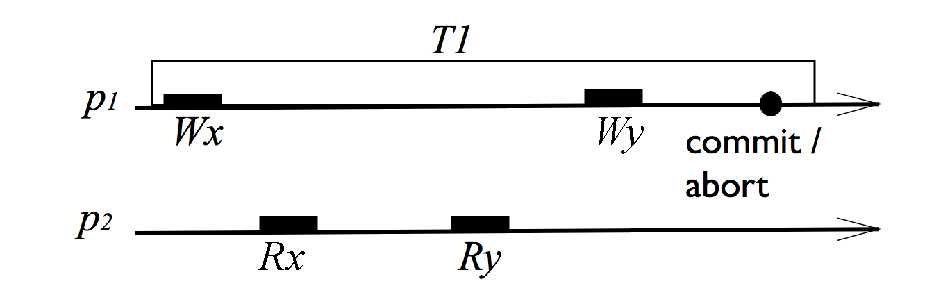
\includegraphics[width=0.4\textwidth]{SI/imgs/non_containment}}     
		%\mbox{\fig{file=imgs/non_containment, width=0.5\textwidth, clip=}}
    \mbox{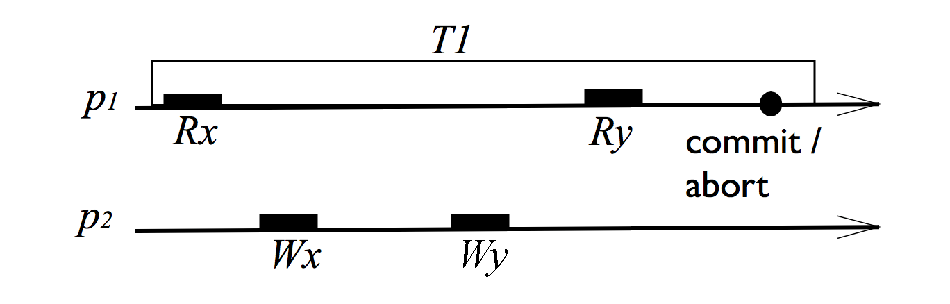
\includegraphics[width=0.4\textwidth]{SI/imgs/interference}}
		%\mbox{\fig{file=imgs/interference, width=0.5\textwidth, clip=}}
}
\caption{Left:  {\it Containment}  (operation $R_x$  should not  return the
    value written to $x$ inside the transaction). 
Right:  {\it  Non-Interference} (wile  it is still  executing, transaction
$T_1$ should not have access to the values that were written to $x$ and $y$
by process $p_2$).} 
\label{fig:int-nonc}
\end{figure*}
%An additional feature of strong isolation, implemented in this paper, 
%is that non-transactional read and write operations never abort. 
%For this reason, it is termed {\it terminating strong isolation}.


%Consider the
%case where a transaction $T$  
%pertaining  to process  $p_1$  reads variable  $x$  through read  operation
%$R_x$, and finds that it contains value  
%$v_1$.  Before $T$  commits, and  after  $R_x$ has  completed, assume  that
%another process $p_2$ modifies $x$  
%by  writing value  $v_2$ to  it through  non-transactional  write operation
%$W_{1x}$. Then, assume that either the  
%same process  $p_2$ or a different process  $p_3$ write non-transactionally
%value $v_1$ to $x$ through operation  
%$W_{2x}$. In  this case, process  $p1$ should have  a means to  detect this
%occurrence and transaction $T$ should  
%not commit, given that otherwise, strong isolation would be violated. 


%Non-interference for  a transaction  $T_1$ can also  be compromised  by 
%interaction between non-transactional  
%operations  and  another  transaction   $T_2$,  as  illustrated  in  Fig.
%\ref{fig:timent}. There, non-transactional operation  
%$R_{2x}$  reads  what transaction  $T_2$  has  written  to shared  variable
%$x$. Due to maintaining consistency, it is not  
%possible  to find  a  correct serialization  order where  non-transactional
%operation $W_y$ does not happen during the  
%duration  of transaction $T_1$,  violating non-interference.  Therefore, in
%order to preserve opacity, this situation would  
%have to  be detected when  transaction $T_1$ attempts to  execute operation
%$R_y$ and $T_1$ would have to be aborted. 
 

%\begin{figure*}[ht]
%\centerline{
%    \mbox{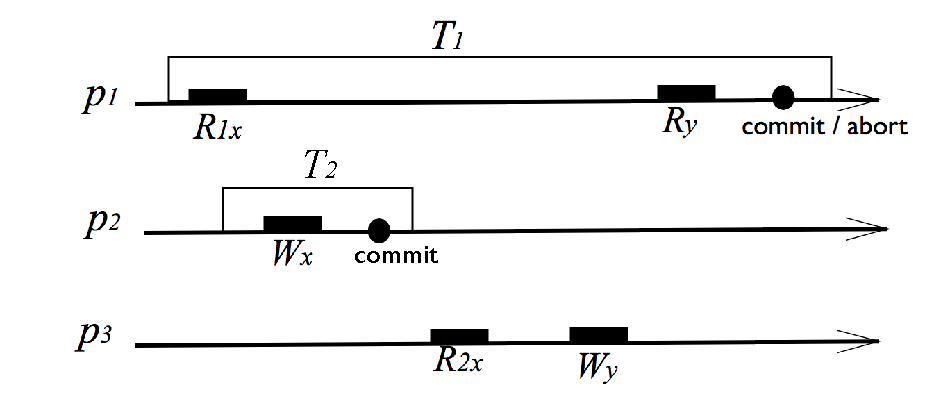
\includegraphics[width=0.5\textwidth]{imgs/time_NT.eps}}
%}
%\caption{Transaction  $T_2$  and  non-transactional operations  of  process
%$p_3$ interfere with transaction $T_1$.} 
%\label{fig:timent}
%\end{figure*}





%========================================================================
\subsection{Terminating Strong  Isolation}
\label{sec:protocol}


Strong isolation allows transactions to not be restricted to use a fixed
subset of memory while still ensuring their atomicity with repect to
other transactions as well as non-transactional operations.
This allows the programmer to preform reads ands write to the same memory he accesses
in his transactions without having to worry about observing or creating inconsistencies.
As indicated in the paragraph on strong isolation, one possible implementation
is to simply convert all non-transactional reads and writes into mini-transactions.
Let us also consider the solution to  the problem of  ensuring strong isolation 
by using  locks or barriers: Each shared
variable would then  
be associated with a lock and both transactions as well as non-transactional 
operations would have to access the lock before accessing the variable.
Locks are already used  in TM algorithms - such as TL2  itself - where it is
however     assumed   that  shared   memory   is   only  accessed   through
transactions. The use  of locks  in a TM algorithm  entails blocking and may
even lead a process to starvation.
Previous research on STM protocols has taken the approach that
these characteristics might acceptable.
The reason for this is that the
programmer  accepts the fact that a  transaction has a duration and that it
may  even  fail: Given that every live transaction has the posibility
to abort means that the  
failure to complete can be considered a part of the transaction concept.  

Now if we have non-transactional operations that rely on the same mechanisms
(either implemnted using locks or by mini-transactions) then they are sucseptable
to the same posibilty of non-completion.
However one must consider that a transaction does not have the same semantics
as a simple read or write operation.
While the concept of the memory  transaction includes the possibility of failure,
the concept of a simple read/write operation does not.
When it  comes to single read or  write accesses  to  a shared
variable, a  non-transactional operation is normally understood  as an
event  that  happens   atomically  and   completes.
While executing, a  read  or write  operation   is  not 
expected  to  be de-scheduled, blocked or aborted.  
Unfortunately   strong
isolation  implemented with  locks  entails the blocking  
of non-transactional read and write operations and would not provide termination.
In the previous chapter we argued that, when considering ease-of-use, 
every transaction should be committed and the
possible non-termination of transactions is unacceptable.
Even worse would be if a programmer had to consider that simple
read and write operations to shared memory are not guaranteed to terminate.
Such an approach to strong isolation would then be rather counter-intuitive for the 
programmer (as well as possibly detrimental for program efficiency).

For this reason we believe that an STM protocol implementing srong
isolation should also consider the progress of non-transactional operations.
In order to deal with this we suggest that a STM protcol should implemnt
\emph{terminating strong isolation}, which we simply define as strong isolation
with the additional guarantee that the non-transactional read and write
operations of a process are guaranteed to terminate no matter the actions of
concurrent processes in the system.
The rest of this chapter will focus on the design of an STM protocol
that ensures terminating strong isolation.

% The non-transactional read and write operations in this algorithm
% focus on efficiency and do not
% rely on locks, instead only executing non-blocking operations with no loops
% ensuring their termination.







% This means that a
% programmer expects  that a transaction  
% might fail,  either by blocking or by  aborting.
% 
% read or write operations, which  the programmer expects to
% be  atomic. 





%Strong isolation always imposes synchronization between 
%transactional and non-transactional code that access memory areas that 
%are potentially shared, which means that a system that guarantees strong 
%isolation is inherently privatization safe.







% \paragraph{Content of the Paper.}
% This paper presents  a TM  algorithm which takes the
% previous issues into account. It is built on top of 
% TM algorithm TL2 \cite{dice06},  a  word-based  TM algorithm  that  uses locks. 
% More precisely,  TL2 is modified to provide strong isolation with non-transactional read 
% and write operations.  However,  
% the algorithm  is designed  without the use  of locks  for non-transactional
% code, in order to guarantee that their execution will always terminate.  
% To achieve  this,    two    additional     functions are specified, which substitute 
% %${\sf non\_transactional\_read()}$ and ${\sf non\_transactional\_write()}$,  
% %which  the programmer  has to  use instead  of 
% conventional  read  or write operations that have to be performed  outside  of  a  transaction.  
% %The  possible ``bad  scenarios''  of  running
% %transactional and non-transactional code in  
% %the absence of strong isolation 
% % Possible violations of correctness under strong isolation are reviewed in Sect. 
% % \ref{sec:badthings}. The TL2 algorithm is described in Sect. \ref{sec:tl2}. 
% % Section \ref{sec:protocol} describes  the proposed algorithm that implements
% % strong isolation for TL2, while  
% % Sect. \ref{sec:conclusions}  concludes the paper by  summarizing the work
% % and examining possible applications.  

% \paragraph{Consistency Issues.}
% 
% % \ignore{When it comes  to environments where shared memory  is 
% % accessed exclusively through transactions, then most accepted  
% % consistency   conditions    build   on   the idea of  {\it serializability}
% % \cite{P79}, a condition first  established  for  the study  of  database  transactions.}
% 
% Commonly, consistency conditions for TM build on the concept of 
% {\it serializability} \cite{P79}, a condition first  established  for  the 
% study  of  database  transactions.
% 
% % \ignore{For a  concurrent
% % execution of transactions to be serializable, it must be  
% % possible to find a serialization for it, i.e., a legal sequential execution
% % that is equivalent to it. }
% 
% A concurrent execution of transactions is serializable, 
% if there exists a serialization, i.e., a legal sequential execution equivalent to it.
% Serializability refers only to committed  transactions,  however, and fails to take into 
% account the possible program exceptions that a TM transaction may cause - even if 
% it aborts - when it observes an inconsistent state of memory.
% 
% % \ignore{  the  context of  memory transactions,  stricter
% % criteria are desirable, because even transactions that  
% % will  eventually abort  may cause  program  exceptions if  they observe  an
% % inconsistent state of the shared memory.  For this  
% % reason, a  prominent consistency condition for  transactional memory, which
% % is stricter than serializability,  has been proposed. }
% 
% {\it Opacity} \cite{guerraoui08}, a stricter consistency condition for TM, 
% requires   that  both committed as well as aborted transactions  
% observe a  consistent state  of shared memory.  This implies that  in order  for a
% concurrent execution of memory transactions to be  
% opaque,  there must exist  an equivalent,  legal sequential  execution that
% includes both committed transactions and aborted  
% transactions, albeit reduced to their read prefix.  Other consistency conditions 
% have also been proposed, such as {\it virtual world consistency}~\cite{IR09}. It is weaker than 
% opacity while keeping its spirit (i.e., it depends on both committed 
% transactions and aborted transactions). 

%\vspace{-0.2cm}



% Traditionally, however, transactions
% are designed to synchronize only with other transactions  
% without considering the possibility of  non-transactional code;
% a program that accesses the same shared memory both transactionally
% and non-transactionally would be considered incorrect.
% A TM system that implements opacity minimally guarantees consistency between transactional
% accesses, however, consistency violations  may  still be  
% possible  in the  presence  of concurrent  non-transactional
% code.

%Traditionally, the same goes for code that is non-transactional: It  
%is not expected from the  programmer to know the synchronization details of
%the transactional memory algorithm that will run  
%concurrently with  her non-transactional code.  
%Therefore, this possibility
%of {\it co-existence of two different paradigms}, as well as  
%the  fact that  transactional memory  is mostly  implemented as  a software
%platform - instead of the transaction abstraction being  
%directly  provided by  the hardware  -  reveal  two different  aspects that
%transactional memory may acquire: In the first aspect,  
%it  is  the  only way  through  which  shared  memory  may be  accessed  by
%concurrent processes.  In the second aspect, which  
%comes into view when it exists alongside non-transactional code, it is just
%another means of achieving synchronization,  
%along with  locks, fences  and other traditional methods.  

%=======================================================================
\section{Implementing terminating strong isolation}
\label{sec:badthings}

As previously described, the goal is to design a protocol in which
non-transactional read and write operations never block or abort
i.e. {\it terminating strong isolation}.
Before diving into the design of a new protocol, let us consider how
this relates to the protocol described in the previousl chapter.
The previous chapter introduced an STM protocol in which every transaction
is guaranteed to commit where the progress of a transaction only depends on
its issuing process.
This helps hide the notion of abort for the programmer, but does
not prevent aborts from happeneing at all.
In fact any transaction is allowed to abort, but only a finite number
of times.
When implementing terminating strong isolation on the other hand we
want to compeltely avoid non-transactional operations from aborting.
The most obvious reason for this is because we want non-transactional reads and write
to behave the same as simple atomic reads and writes.

The second, less theoretically intersting, but just as important reason
is performance.
To the programmer the non-transactional operations as simple reads and
writes, he should be able to assume that they are efficient.
In fact, the primary concern of previous research on strong isolation
is performance, it has even been suggested that 

In the previous chapter we were more interested in showing that a concept was
possible, while in this chapter performace is a just as important concern.
Given this we cannot simply implement non-transactional
operations as we did transactions in the previous chapter's protocol.

Still it is not necessary to design a completely new protocol, instead we
choose to take the base design of an efficient state-of-the-art STM protocol
that provides weak isolation and extend it to provide terminating strong isolation.
The TL2 protocol was choosen for this as it is fairly straightforward
and can be considered as one of the fastest STM implementations.
In the redesigned TL2 protocol presented in this chapter
 read   and write operations that appear inside a 
transaction follow the original TL2 algorithm rather closely (cheap read 
only transactions, commit-time locking, write-back), 
with the addition of non-transactional read and  write operations 
that are to be used 
by the programmer, substituting conventional
shared memory read and write operations in order to provide
terminating strong isolation. 

% TM with strong isolation has also been proposed in
% software \cite{SMSA08,shpeis07} in hardware \cite{MTCM07}, and has been suggested to be too costly \cite{DS09}.
% This work differs from other implementations in that it is terminating and
% is implemented on top of a state-of-the-art STM in order to avoid too much extra cost.



%========================================================================
\section{A Brief Presentation of TL2}
\label{sec:tl2}

%This section presents the main  aspects of the  TM algorithm TL2  which  are  
%used by the proposed algorithm. TL2 has been introduced by Dice, Shalev and Shavit 
%in    2006    \cite{dice06} and does not allow for  non-transactional code.  We describe 
%here the word-based version of TL2. In this  version it is considered that shared  memory 
%is accessed in the granularity of  single  memory words.  
%For the sake of  clarity and without loss  of generality, the rest of the description  
%assumes that shared variables are the size of a  memory word. 
%Therefore, the operations issued by a transaction are simply read and write operations. 
%For the sake of brevity, implementation details of the algorithm are omitted.  

TL2, aspects of which are used in this paper, has been introduced by Dice, Shalev and Shavit in 2006 \cite{dice06}.
The word-based version of the algorithm is used, %which means that the shared variables accessed are memory 
%words and that the operations issued by a transaction are simply read and write operations. 
%For the sake of brevity, implementation details of the algorithm are omitted in the following description. 
where transactional reads and writes are to single memory words.
Instead of presenting the detailed alorithm we will only present the main concepts of the algorithm
that are used in the protocol presented in this chapter.
The safety condition ensure by TL2 for transactions is opacity.
It should be noted that the original version of TL2 takes no consideration into non-transactional memory
accesses taking the view that transactions should be relegated to their own separate section of memory.
Extended versions of TL2 that are privitizaion safe have also been exaimed \cite{DSS10}.
%\vspace{-0.25cm}
%---------------------------------------------------------------------
%\subsection{Main Features of TL2}
\paragraph{Main Features of TL2.} The shared variables  that a  transaction reads form its {\it read
set}, while the variables it updates form the {\it write set}. 
Read operations in TL2 are {\it invisible},  meaning  that when  a  transaction reads  a  shared 
variable,  there is no indication of the read to other transactions.  Write operations are  
{\it deferred}, meaning that  TL2 does not perform the updates  as soon as  it {}``encounters'' 
the shared  variables that  it has to write to. Instead, the 
updates it has to perform are logged into a local list (also called {\it redo log}) and   are  applied 
to the shared  memory only once the transaction is certain  to commit.

One of the key features of TL2 is that read-only transactions are considered efficient.
This is because they do not need to maintain 
local copies of a read or write set  and because if they reach the $try\_to\_commit$
operation before aborting then they can commit immediately as they are guaranteed
to be consistend.
To control transaction synchronization, TL2 employs locks and logical dates. 
%The variables  that a  transaction has to read form its read
%set, while the variable it has to update, form its write set.  
%A  transaction  first  has to  obtain  the  locks  that correspond  to  the
%variables of its write set, before it can  
%update them.  Conversely, a  transaction has to  check the logical dates  of the
%variables in its read set, in  
%order to  ensure that  the values  it has read  correspond to  a consistent
%snapshot of shared memory.  



\paragraph{Locks and Logical Date.}
A lock and a logical date is associated with each shared variable.  
TL2 implements logical time as an integer counter denoted $\mathit{GVC}$.
%$\mathit{GVC}$ is incremented by update transactions when they attempt to commit. 
When a transaction starts it reads the current value of $\mathit{GVC}$ into local variable, $\mathit{rv}$. 
This value is used in order to ensure the transaction views a consistent state of memory.

When a transaction attempts to commit it  first  has to  obtain  the  locks  of all the
variables in its write set, before it can  
update them.
Furthermore, a  transaction has to  check the logical dates  of the
variables in its read set in  
order to  ensure that  the values  it has read  correspond to  a consistent
snapshot of shared memory.
Its read set is valid if the logical date of every  item in the set is less than the transaction{}'s $\mathit{rv}$  value. 
If, on the  contrary, the logical date of a read set  item is larger than the $\mathit{rv}$ 
of the transaction,  then  a concurrent  transaction 
has updated this item, invalidating the read.
A transaction must abort if its read set is not valid.  
Once the read set it varified to be consistent the commit operation performs an increment-and-fetch on $\mathit{GVC}$, and stores the 
return value in local variable $\mathit{wv}$ (which can be seen as a write version number  or a version timestamp). 
Should the transaction commit, it will assign its $\mathit{wv}$ as the new logical date of the shared variables in its write set.
Finally the locks are realeased completing the commit operation.

A read operation must check both the lock and the logical time of the variable it is reading.
If it is either locked, or the value of the logical time is greater then $\mathit{rv}$ then the transaction must abort,
otherwise the read is consistent and the value can be returned.
Additionally, if the transaction is an update transaction then the variable is also added to the read set.
Importantly, thanks to the use of the logical clocks the read operations take constant time
and do not require validating the locations previously read in order to ensure opacity.

% \paragraph{Locks.}
In order to implemnt the locks and logical time, they  are stored in  a shared array
of words.
Each shared memory  word accessed by the STM protocol is
mapped to a location in the lock array through a  
one-to-many hash function,  resulting in one
lock covering several shared  
memory locations. This  partitions the memory into  so-called stripes. 
For each memory word in the array
the first bit acts as lock  bit, indicating whether the lock  is free or
not. The rest of the bits form the  
logical time of the variables assoiated to that location by the hash function.


%Timestamping with logical dates facilitates read set validation for a transaction. 
%When the read set of a transaction is not valid,  the transaction  cannot commit. 
%The  read set of  a transaction $T_A$ will be  invalidated  if another,  concurrent 
%transaction $T_B$ modifies shared  variable $x$ and commits, after $T_A$  has 
%read $x$  but while $T_A$ is  still active. 
%In TL2, it  can be detected that a transaction{}'s read  set is valid if 
%has performed  an   increment-and-fetch    of   $\mathit{GVC}$,   updated   the item  and  
%committed,  by  writing  the  new $\mathit{GVC}$ value into the item{}'s  logical date field.

%\paragraph{Update vs Read-only Transactions.}
%A {\it read-only} transaction in TL2 consists  of a  begin phase and  an operation phase.  
%An {\it update}  transaction has an additional commit phase. In  an update transaction, 
%the operation phase will contain write operations to shared variables as well as possibly 
%read operations, while  in a  read-only transaction, it  will solely contain read  operations. 
%Read operations in TL2 are {\it invisible},  meaning  that when  a  transaction reads  a  shared 
%variable,  there is  no indication of that fact towards  other transactions.  Write operations are  
%{\it deferred}, meaning that  TL2 does not perform the updates  as soon as  it {}``encounters'' 
%the shared  variables that  it has to write to (i.e., during the operation  phase). Instead, the 
%updates it has to perform are logged into a local list (also called  redo log) and   are  applied 
%to the shared  memory only once the transaction is certain  to commit (i.e. which occurs  during the
%commit phase). 


%\paragraph{Logical Time.}
%TL2 implements logical time as an integer counter denoted $\mathit{GVC}$.
%It is incremented by update transactions when they attempt to commit. 
%When it starts up, a transaction reads the current value of $\mathit{GVC}$ into local variable, $\mathit{rv}$. 
%When a transaction attempts to commit, it performs an increment-and-fetch on $\mathit{GVC}$, and stores the 
%return value in local variable $\mathit{wv}$ (which can be seen as a write version number  or a version timestamp). 
%Should the transaction commit, it will assign its $\mathit{wv}$ as the new logical date of the shared variables in its write set. 

%Timestamping with logical dates facilitates read set validation for a transaction. 
%When the read set of a transaction is not valid,  the transaction  cannot commit. 
%The  read set of  a transaction $T_A$ will be  invalidated  if another,  concurrent 
%transaction $T_B$ modifies shared  variable $x$ and commits, after $T_A$  has 
%read $x$  but while $T_A$ is  still active. 
%In TL2, it  can be detected that a transaction{}'s read  set is valid if the logical date 
%of every  item on the read set is less than the transaction{}'s $\mathit{rv}$  value. 
%If, on the  contrary, the logical date of a read set  item is larger than the $\mathit{rv}$ 
%of the transaction,  then this  indicates that,  in the meanwhile,  a concurrent  transaction 
%has performed  an   increment-and-fetch    of   $\mathit{GVC}$,   updated   the item  and  
%committed,  by  writing  the  new $\mathit{GVC}$ value into the item{}'s  logical date field.



%========================================================================
%\subsection{Inside a TL2 Transaction}
%\subsection{TL2 Read and Write Operations}
%\paragraph{TL2 Read and Write Operations}
%\paragraph{Begin of a Transaction.}
%When a  transaction starts  up, it  reads the current  value of  the $\mathit{GVC}$ 
%and stores it into  its local  $\mathit{rv}$ variable. %A transaction  has to keep  track of the
%variables in its read set and their  versions, as well as the variables in  its write set and 
%values that it has to write to them. Therefore, it  implements the  read and  write set  as 
%local lists,  which will  be filled during the transaction execution.  
%These data structures are also initialized at start-up.
%\begin{itemize}
%\paragraph{TL2 Write Operation.}
%\item When a transaction  has to update shared variable $x$, % it creates an entry
%for it in its local write set list  
%and there, it  stores $x${}'s address and the value that  has to be written to it.  
%it performs the intended update on the variable{}'s local copy in the transaction{}'s 
%redo log. If the transaction commits, the update will be performed during the commit phase.

%\paragraph{TL2 Read Operation.}
%\item When  a transaction has  to read  shared variable  $x$, then,  if it  is an
%update transaction, it first explores  its redo log in order to check whether $x$ is already contained
%there. Should this be the case,  then, in order to preserve consistency,  the value that is contained in the
%write set list will be returned for  the variable.  Otherwise, or in case it is read-only, a transaction checks 
%the lock and logical date of $x$ before and after reading it. If these checks determine that $x$ is not 
%concurrently updated by another transaction and reading it doesn{}'t invalidate the read set, the transaction 
%proceeds. Otherwise it aborts. 
%\end{itemize}
%Before and after reading $x${}'s value, a read-only transaction samples the
%lock bit and the lock version  
%corresponding to $x$. If the lock version is different before and after the
%read or if the lock bit is set, then  
%the transaction aborts, given that it has just detected a concurrent update
%of $x$ which invalidates its read  
%set.  If this  procedure, also  referred  to as  post-validation, does  not
%result in aborting, then the operation can   
%return the value that it has read  for $x$. If the transaction is an update
%transaction, then, before returning the  
%value, it  creates an entry for  $x$ in its  local read set list,  where it
%stores the memory address of $x$.  

%\paragraph{Attempt to Commit.}
%After  having executed  all its  read and/or  write operations, a transaction attempts  
%to commit. If  it is a read-only transaction, it has a consistent read set already and 
%commits without further explicit action. An update  transaction has to explicitly verify 
%whether it can commit by checking if it{}'s read set is still consistent. Then, in order 
%to make its updates  visible  to  the rest  of  transactions, it has to obtain the locks of 
%all variables in its write set and then update their values and their logical timestamps. 
%The logical timestamp is updated to the value of $wv$, which in turn is obtained by 
%performing an  increment-and-fetch  on $\mathit{GVC}$. The transaction commits 
%by releasing the locks again.


%\paragraph{Lock Acquisition and $\mathit{GVC}$ Increment.} 
%For  every item  in  the  transaction{}'s write  set,  bounded spinning  is
%performed on the corresponding lock in order  
%to  obtain  it.  If the  lock  acquisition  for  an  item fails,  then  the
%transaction aborts. If, however, all locks are acquired  
%successfully,   then  the   transaction  performs   increment-and-fetch  on
%$\mathit{GVC}$ and stores the return value in  
%local variable $\mathit{wv}$. This value of $\mathit{wv}$ will be stored as
%the new version of the variables in the  
%transaction's write set, if the transaction does not abort.

%\paragraph{Validation of the Read Set.}
%In order  to determine whether the  transaction has to abort,  a final read
%set validation takes place. During this  
%validation, it  is verified  for all  items of the  read set  whether their
%current version is still less that the transaction's  
%read version, $\mathit{rv}$, as well as whether the items are not locked by
%a different transaction. If it is detected  
%that this is not the case  for any item, the transaction aborts. Otherwise,
%the transaction can perform the intended  
%updates. Read  set validation  is not necessary  in the special  case where
%$\mathit{rv}$+1 = $\mathit{wv}$, given  
%that this would  guarantee that no concurrent transaction  has executed and
%possibly modified items of the read   set in the meanwhile.

%\paragraph{Deferred Updates and Lock Release.}
%The   address  and   update  value   for  each   shared  variable   in  the
%transaction{}'s write set is stored in a corresponding  
%entry  in the  transaction{}'s local  write set  list. Therefore,  for each
%write set list entry, the update value is stored in the  
%corresponding memory address. The  locks are released by atomically writing
%the value of $\mathit{wv}$ to their lock  
%version field  while clearing the lock bit. 



\section{The Protocol}

The following sections will describe the protocol.
%===================================================================
\subsection{Memory Set-up and Data Structures.}


\paragraph{Memory Set-up.}
The underlying memory system is made up of atomic read/write registers. 
Moreover some of them can also be accessed by the the following two 
operations. The operation denoted 
${\sf Fetch\&increment}()$ atomically adds one to the register and 
returns its previous value. 
 The operation denoted 
${\sf C\&S}()$ (for compare and swap) is a conditional write. 
${\sf C\&S}(x,a,b)$ writes $b$ into $x$ iff $x=a$. In that case it 
returns $\mathit{true}$. Otherwise it returns  $\mathit{false}$. 


The proposed algorithm assumes that the
variables  are  of  types and  values  that  can  be   stored in  a  memory
word. This assumption aids in the clarity of the algorithm description  
but it  is also  justified by the  fact that  the algorithm extends  TL2, an
algorithm that is   designed to be word-based. 

As in TL2,  the variable $\mathit{GVC}$
acts as  global  clock  which  is incremented  by update transactions.
 Apart from a global   notion of ``time'', there exists also
a local one; each process maintains a local  
variable denoted $\mathit{time}$,  which is used in order to keep  
track of when, with
respect to the $\mathit{GVC}$, a non-transactional operation 
or a transaction was last performed by
the  process.
This variable is then used during non-transactional operations to ensure
the (strict) serialization of operations is not violated.
% Each  process's  $\mathit{time}$   variable is   
% therefore incremented
% both during transactional and non-transactional operations.

As described in section \ref{sec:tl2}, in TL2 a  shared array of locks is maintained and each
shared memory word  
is associated with a lock in this array by some function. Given this, a memory
word directly contains  
the value of the variable that  is stored in it.
Instead, the algorithm presented here, uses
a  different memory set-up that does not require a lock array, but does require
an extra level of indirection when loading and storing values in memory.
Instead of storing the value of a variable directly to a memory word,
each  write  operation  on  variable  $\mathit{var}$,   transactional  or
non-transactional, first creates an algorithm-specific   
structure that contains the new value of  $\mathit{var}$, as
well as necessary meta-data and second stores a pointer to this structure in the memory word.
The memory set-up  is illustrated in Fig.  \ref{fig:mem_setup}.
Given the particular memory arrangement  that the algorithm uses,
pointers are used in order to load and store items from memory.
\footnote{The following  notation  is
used. If $pt$ is a pointer, $pt\downarrow$ is the object pointed to by $pt$. 
if $aa$ is an object, $\uparrow aa$ is a pointer to $aa$. Hence 
$((\uparrow aa)\downarrow =aa$ and $ \uparrow(pt \downarrow)=pt$.}


\paragraph{T-record  and NT-record.}
These  algorithm-specific  data structures  are shared  and  can be  of 
either  two  kinds, which will be referred   to as T-records and NT-records. 
A T-record is created by a transactional write operation while an 
NT-record is created by a  non-transactional write operation.
%  A memory word
% that is used to store  
% variable $\mathit{var}$ at address $\mathit{addr}$ will then contain a pointer to a  
% record of either of the  aforementioned types and within this structure
% the actual value for  $\mathit{var}$ is stored as a field. 


\begin{figure*}[ht]
\centerline{
    \mbox{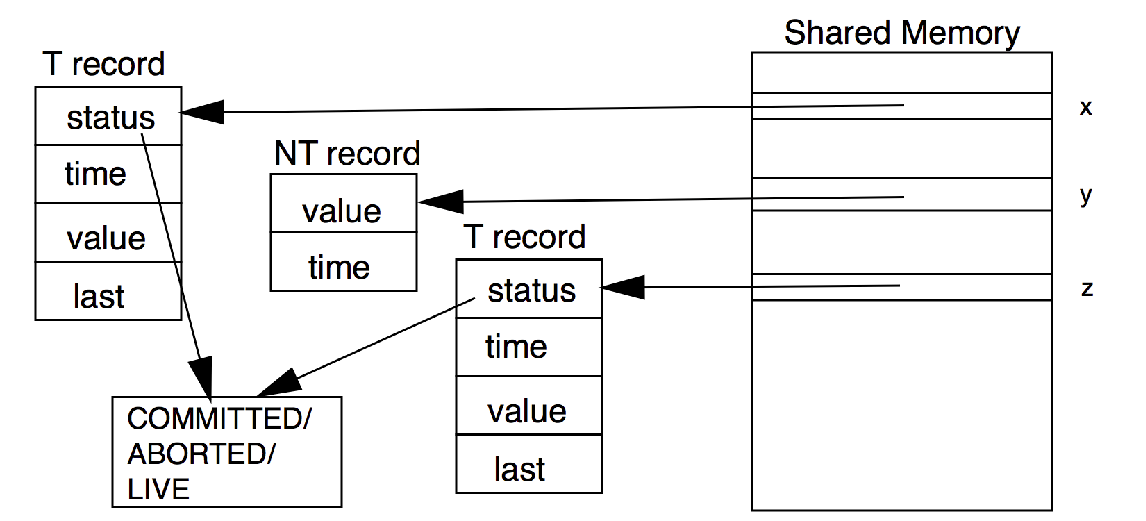
\includegraphics[width=0.6\textwidth]{SI/imgs/mem_setup_single}}
}
\caption{The memory set-up and the data structures that are used by the 
algorithm.}
\label{fig:mem_setup}
\end{figure*}

New T-records are created during the transactional write operations.
Then during
the commit operation the pointer stored at $\mathit{addr}$ is updated to point to this new T-record.
During NT-write operations new NT-records are created and the pointer at $\mathit{addr}$
is updated to point to the records.

When a read operation - be it transactional or non-transactional - accesses 
a shared variable it cannot know beforehand what type of record it will find. 
Therefore, it can be seen in the algorithm listings, that whenever 
a record is accessed, 
the operation checks its type, i.e., it checks 
whether it is a T-record or an NT-record (for example, line \ref{A02} in Fig.
\ref{fig:ntops} contains such a check. A T-record is {}``of type T'', while an 
NT-record is {}``of type NT''). 


\paragraph{T-record.}
A T-record is a structure containing the following fields.
\begin{description}
%\vspace{-0.1cm}
\item[$\mathit{status}$] This  field  indicates  the  state  of the  transaction  that  created  the
T-record. The  
state can either be LIVE, COMMITTED or ABORTED.
The state is initially set to LIVE and is not set to COMMITTED until during the commit operation when 
all locations of the transaction's write set have been set to point to the transaction's T-records
and the transaction has validated its read set.
Since a transaction can write to multiple locations, the $\mathit{status}$ field
does not directly store the state, instead it contains a
pointer to a memory location containing the state for the transaction.
Therefore the $\mathit{status}$ field of each T-record created by the same transaction will point to the same location.
This ensures that any change to the transaction's state is immediately recognized at each record.
%\vspace{-0.2cm}
\item[$\mathit{time}$] The  $\mathit{time}$  field of  a T-record  contains the  
value of  the $\mathit{GVC}$  at  the  moment the  record  was 
inserted to memory. %  into the  list of   records.
This is similar to the logical dates of TL2.
%\vspace{-0.2cm}
\item[$\mathit{value}$] This field contains the value that is meant to be written to the chosen 
memory location.
%\vspace{-0.2cm}
\item[$\mathit{last}$] During the commit operation, locations are updated to point
to the committing transaction's T-records, overwriting the previous value
that was stored in this location.
Failed validation or concurrent non-transactional operations may cause this transaction to abort 
after it updates some memory locations, but before
it fully commits.
Due to this, the previous value of the location needs to be available for future reads.
Instead of rolling back old memory values, the $\mathit{last}$ field of a T-record is used,
storing the previous value of this location.

\end{description}


\paragraph{NT-record.}
An NT-record is a structure containing the following fields.
\begin{description}
%\vspace{-0.1cm}
\item[$\mathit{value}$]
This field contains the value that is meant to be written to the chosen 
memory location.
%\vspace{-0.2cm}
\item[$\mathit{time}$]
As in the case of T-records, the $\mathit{time}$ field of NT-records 
also stores the value 
of the $\mathit{GVC}$ when the write took place.
%This field is 
%used to avoid inconsistencies %such as the ones illustrated by Figure 
%\ref{fig:timent}. 
%caused by the ABA problem.
\end{description}

Due to this different memory structure a shared lock array is no longer needed,
instead of locking each location in the write set during the commit operation, this algorithm
performs a compare and swap directly on each memory location changing the address to point to one of its T-records.
After a successful compare and swap
 and before the transactions status has been set to COMMITTED or ABORTED, the transaction effectively
owns the lock on this location.
Like in TL2, any concurrent transaction that reads the location and sees that it is locked ($\mathit{status} = $ LIVE) will
abort itself.

% During read operations (transactional or non-transactional) the additional data in these structures is used 
% to determine the most  recent valid value  of a variable.
% Should the item be of type NT-record,
% then it's $\mathit{value}$ field contains the most  
% recent valid value  of the variable. On the other hand,  should the item
%  be a  T-record, then if the $\mathit{status}$ field of
% the record is equal to COMMITTED,  
% the $\mathit{value}$ field represents the current value of the variable. Otherwise, the
% $\mathit{last}$ field contains the current value.

\paragraph{Transactional Read and Write Sets.}
Like TL2, read only transactions do not use read sets while update transactions do.
The read set is made up of a set of tuples for each location read, $\tuple{\mathit{addr, value}}$
where $\mathit{addr}$ is the address of the location read and $\mathit{value}$ is the value.
The write set is also made up of tuples for each location written by the transaction,
$\tuple{\mathit{addr, item}}$ where $\mathit{addr}$ is the location to be written
and $\mathit{item}$ is a T-record for this location.

\subsubsection{Discussion.}
One advantage of the TL2 algorithm is in its memory layout.
This is because reads and writes happen directly to memory (without indirection)
and the main amount of additional memory that is used is in the lock array.
Unfortunately this algorithm breaks that and requires an additional level of indirection
as well as additional memory per location.
While garbage collection will be required for old T- and NT-records, here we assume
automatic garbage collection such as that provided in Java, but additional solutions will be explored in future work.
These additional requirements can be an acceptable trade-off given that they are only
needed for memory that will be shared between transactions.
In the appendix of this paper we present two variations of the algorithm that trade
off different memory schemes for different costs to the transactional and
non-transactional operations.


%====================================================================

\subsection{Description of the Algorithm.}

The main goal of the algorithm is to provide strong isolation 
in such a way that  the non-transactional  operations are never blocked or aborted. 
In order  to achieve this,  the algorithm delegates most of its
concurrency   control   and  consistency   checks   to  the   transactional
code. Non-transactional  
operations access and modify  memory  locations without waiting for concurrent transactions
 and it is mainly up to transactions accessing the same location to
deal with ensuring safe concurrency.  As a
result, this algorithm gives high  priority   to non-transactional code. 

%=====================================================================
\subsection{Non-transactional Operations.}
Algorithm-specific  read  and write operations
shown in Fig. \ref{fig:ntops} must be used when a shared variable is accessed
accessed outside of a transaction.
As described in section \ref{sec:SIsolutions} this can be done by hand by the programmer,
but more appropriately a programmer will write normal shared reads and writes which will then
be automatically converted to non-transactional read (resp. write) operations by
the compiler or dynamically at runtime.

\begin{figure}[htb]
\centering{ \fbox{
\begin{minipage}[t]{1\linewidth}%{150mm}
%\footnotesize 
\scriptsize
\renewcommand{\baselinestretch}{2.5} 
%\resetline
%\setcounter{linecounter}{200}
\begin{tabbing}
aaaaaaa\=aa\=aaaaa\=aa\=aa\=\kill %~\\


{\bf operation}  ${\sf non\_transactional\_read}(\mathit{addr})$ {\bf is}\\
\line{A01} \> $\mathit{tmp} \gets (\downarrow \mathit{addr})$; \\ 
\line{A02} \> {\bf if} $( ~\mathit{tmp}$ is of type T $ \wedge (\downarrow \mathit{tmp.status}) \neq$ COMMITTED ) \\
\line{A03}  \>\>  {\bf then if}  $(\mathit{tmp.time}  \leq \mathit{time}  \wedge  (\downarrow \mathit{tmp.status}) = $ LIVE) \\
\line{A04} \>\>\>\> {\bf then} \=${\sf \mathit{C\&S}}$($tmp.status$, LIVE, ABORTED) {\bf end if}; \\
%\line{A05} \>\> {\bf end if} \\
\line{A06} \>\>\> {\bf if} ($(\downarrow \mathit{tmp.status}) \neq $ COMMITTED)  \\
\line{A07} \>\>\>\> {\bf then} $\mathit{value} \gets \mathit{tmp.last}$ \\
\line{A08} \>\>\>\> {\bf else} $\mathit{value} \gets \mathit{tmp.value}$ \\
\line{A05} \>\>\> {\bf end if}; \\
\line{A09} \>\> {\bf else} $\mathit{value} \gets \mathit{tmp.value}$ \\
\line{A09A} \> {\bf end if}; \\
\line{A10} \> $\mathit{time} \gets {\sf max}(\mathit{time}, \mathit{tmp.time})$ \\
\line{A11} \> {\bf if} ($\mathit{time} = \infty$) {\bf then} $\mathit{time} = \mathit{GCV}$ {\bf end if}; \\
\line{A12} \> ${\sf return}$ ($\mathit{value}$) \\
{\bf end operation}. \\
\\
{\bf operation}  ${\sf non\_transactional\_write}(\mathit{addr, value})$ {\bf is}\\
\line{B01} \> allocate new variable $\mathit{next\_write}$ of type NT; \\
\line{B02} \> $\mathit{next\_write} \gets \mathit{(addr, value, \infty)}$; \\
\line{B03} \> $\mathit{addr} \gets (\uparrow \mathit{next\_write})$ \\
\line{B04} \> $\mathit{time} \gets \mathit{GVC}$; \\
\line{B05} \> $\mathit{next\_write.time} \gets \mathit{time}$; \\
{\bf end operation}.

\end{tabbing}
\normalsize
\end{minipage}
}
\caption{Non-transactional operations for reading and writing a variable.}
\label{fig:ntops}
}
\end{figure}

\paragraph{Non-transactional Read.}
The   operation  ${\sf   non\_transactional\_read()}$  is   used   to  read,
when not in a transaction, the value stored at
$\mathit{addr}$.
The  operation first  dereferences  the pointer  stored at  $\mathit{addr}$
(line \ref{A01}).
If the item is a T-record that was created by a 
transaction which  has not yet  committed then the $\mathit{value}$ field
cannot be immediately be read as the transaction might still abort.
Also if the current process has read (or written to) a value that is more recent then the transaction
(meaning the process's $\mathit{time}$ field is greater or equal to the T-records
$\mathit{time}$, line \ref{A03}) then the transaction must be directed to abort (line \ref{A04})
so that opacity and strong isolation (containment specifically) is not violated.
From a T-record with a transaction that is not committed, the value from the $\mathit{last}$
field is stored to a local variable (line \ref{A07}) and will be returned on operation completion.
Otherwise the $\mathit{value}$ field of the T- or NT-record is used (line \ref{A08}).

% Once  the correct value  has been  found  and stored  in local  variable 
% $\mathit{value}$, the local $\mathit{time}$   
% variable  is updated  (lines \ref{A10}-\ref{A11}).  The updated  $\mathit{time}$
% value is used by non-transactional operations and is necessary in order to allow 
% the detection of consistency 
% violations such as the one illustrated by Figure \ref{fig:timent}. 
% By advancing the value of $\mathit{time}$ 
% through a non-transactional read operation, 
% the serialization order of this read operation with 
% respect to transactional or non-transactional operations 
% that it read from is reflected.

Next the process local variable $\mathit{time}$ is advanced to 
the maximal 
value among its current 
value and the logical date of the T- or NT-record whose value was read.
Finally if $\mathit{time}$ was set to $\infty$ on line \ref{A10}
(meaning the T- or NT-record had yet to set its $\mathit{time}$), then it is updated
to the $\mathit{GCV}$ on line \ref{A11}.
The updated  $\mathit{time}$
value is used 
%by non-transactional operations and is necessary 
to prevent consistency 
violations. %such as the one illustrated by Figure \ref{fig:timent}. 
%caused by the ABA problem.
Once these book-keeping 
operations are finished, the local variable $\mathit{value}$
is returned (line \ref{A12}).

\paragraph{Non-transactional Write.}
The operation ${\sf non\_transactional\_write()}$ is used to write to 
a shared variable $\mathit{var}$ 
by non-transactional code.
The operation takes as input the address of the shared variable as well as the 
value to be written to it.
This operation  
creates a  new  NT-record  (line  \ref{B01}),  fills  in  its  fields  (line
\ref{B02})  and 
changes the pointer stored in $\mathit{addr}$ so that it references the 
new record it has created  (line \ref{B03}).
Unlike update transactions, non-transactional writes do not increment
the global clock variable $\mathit{GCV}$.
Instead they just read $\mathit{GCV}$ and set the NT-record's time value as well as
the process local $\mathit{time}$ to the value read (line \ref{B04} and \ref{B05}).
Since the $\mathit{GCV}$ is not incremented, several NT-records might have the same
$\mathit{time}$ value as some transaction.
When such a situation is recognized where a live transaction has the same time value
as an NT-record the transaction must be aborted (if recognized during an NT-read operation,
line \ref{A04}) or perform read set validation (if during a transactional
read operation, line \ref{C05} of Fig. \ref{fig:tops}).
This is done in order to prevent consistency violations
caused by the NT-writes not updating the $\mathit{GCV}$. %such as the one shown in Figure \ref{fig:timent}.

%==================================================================
\subsection{Transactional Read and Write Operations.}

The transactional operations for performing reads and writes are 
presented in Fig. \ref{fig:tops}. 

\paragraph{Transactional Read.}

The operation ${\sf  transactional\_read()}$ takes $\mathit{addr}$ as
input. It starts by checking  
whether the  desired variable already  exists in the  transaction{}'s write
set, in which  
case  the   value  stored there  will   be  returned  (line
\ref{C01}). If the variable is not contained  
in  the write  set, the  pointer in  $\mathit{addr}$ is  dereferenced (line
\ref{C02}) and set to $\mathit{tmp}$. Once this is detected to be a T- or NT-record
some checks are then performed in order to ensure correctness.

In the case that $\mathit{tmp}$ is a T-record the operation must check to see
if the status of the transaction for this record is still LIVE and if it is
the current transaction is aborted (line \ref{C10}).
This is similar to a transaction in TL2 aborting itself when a locked location is found.
Next the T-record's $\mathit{time}$ field is checked, and (similar to TL2) if it 
greater then the process's local $\mathit{rv}$ value the transaction must abort 
(line \ref{C12}) in order to prevent consistency violations.
If this succeeds without aborting then the local variable $\mathit{value}$
is set depending on the stats of the transaction that created the T-record (line \ref{C10}-\ref{C11}).

In case $\mathit{tmp}$ is an 
NT-record (line \ref{C03}), the operation
checks whether the value of the $\mathit{time}$ field is
greater or equal to the process local $\mathit{rv}$ value.
If it is, then this write has possibly occurred after the start of this
transaction and there are several possibilities.
In the case of an update transaction validation must be preformed, ensuring
that none of the values it has read have been updated (line \ref{C05}).
In the case of a read only transaction, the transaction
is aborted and restarted as an update transaction (line \ref{C06}).
It is restarted as an update transaction so that it has a read set that it can validate
in case this situation occurs again.
Finally local variable $\mathit{value}$ is set to be the value
of the $\mathit{value}$ field of the $\mathit{tmp}$ (line \ref{C07}).

It should be noted that the reason why the checks are performed differently
for NT-records and T-records is because the NT-write operations do not
update the global clock value while update transaction do.
This means that the checks must be more conservative in order to ensure correctness.
If performing per value validation or restarting the transaction as an update transaction
is found to be too expensive, a third possibility would be to just increment the global
clock, then restart the transaction as normal.

Finally to finish the read operation, the $\tuple{\mathit{addr, value}}$
is added to the read set if the transaction is an update transaction (line \ref{C14}),
and the value of the local variable $\mathit{value}$  is returned.

\begin{figure} [htb]
\centering{ \fbox{
\begin{minipage}[t]{1\linewidth}%{150mm}
%\footnotesize 
\scriptsize
\renewcommand{\baselinestretch}{2.5} 
%\resetline
%\setcounter{linecounter}{200}
\begin{tabbing}
aaaaaaa\=aa\=aaaaa\=aa\=aa\=\kill %~\\


{\bf operation}  ${\sf transactional\_read}(\mathit{addr})$ {\bf is}\\
\line{C01} \> {\bf if} $\mathit{addr} \in \mathit{ws}$  {\bf then} ${\sf return}$ ($\mathit{item.value}$ from $\mathit{addr}$ in $\mathit{ws}$)  {\bf end if}; \\
\line{C02} \> $\mathit{tmp} \gets (\downarrow \mathit{addr})$; \\

\line{C03} \> {\bf if} ($\mathit{tmp}$ is of type NT)   \\
\line{C04} \>\> {\bf then} {\bf if} ($\mathit{tmp.time} >= \mathit{rv}$) \\
%\> \% Do validation to prevent abort due to a non-transactional write \\
\line{C05} \>\>\> {\bf then if} this is an update transaction {\bf then} ${\sf validate\_by\_value}$() \\
\line{C06} \>\>\>\>\> {\bf else} ${\sf abort}$() and restart as an update transaction {\bf end if}; \\

\line{C06A} \>\>\> {\bf end if}; \\
\line{C07} \>\>\> $\mathit{value} \gets \mathit{tmp.value}$; \\

\line{C08} \>\> {\bf else} \\
\line{C09} \>\>\> {\bf if} ($(\mathit{status} \gets (\downarrow \mathit{tmp.status})) \neq$ COMMITTED $)$ \\
\line{C10} \>\>\>\> {\bf then if} ($\mathit{status} =$ LIVE) {\bf then} ${\sf abort}()$  {\bf else} $\mathit{value} \gets \mathit{tmp.last}$ {\bf end if}; \\
\line{C11} \>\>\>\> {\bf else} $\mathit{value} \gets \mathit{tmp.value}$ \\
\line{C11A} \>\>\> {\bf end if}; \\
\line{C12} \>\>\> {\bf if} $(\mathit{tmp.time} > \mathit{rv})$ {\bf then} ${\sf abort}()$ {\bf end if}; \\
\line{C13} \> {\bf end if}; \\

\line{C14} \> {\bf if} this is an update transaction 
                        {\bf then} add $\tuple{\mathit{addr,value}}$ to $\mathit{rs}$ {\bf end if}; \\
\line{C15} \> ${\sf return}$ ($\mathit{value}$) \\
{\bf end operation}. \\
\\
{\bf operation}  ${\sf transactional\_write}(\mathit{addr, value})$ {\bf is}\\
\line{D01} \> {\bf if} $\mathit{addr} \not\in \mathit{ws}$  \\
\line{D02} \>\> {\bf then} \> allocate a new variable $item$ of type $T$; \\
\line{D03} \>\>\> $\mathit{item}  \gets (\mathit{value, (\uparrow status), \infty})$; 
                   $\mathit{ws} \gets \mathit{ws} \cup \tuple{\mathit{addr, item}}$; \\
\line{D04} \>\> {\bf else} \> set $\mathit{item.value}$ with $\mathit{addr}$ in $\mathit{ws}$ to $\mathit{value}$ \\
\line{D05} \> {\bf end if}; \\
{\bf end operation}.
\end{tabbing}
\normalsize
\end{minipage}
}
\caption{Transactional operations for reading and writing a variable.}
\label{fig:tops}
}
\end{figure}

\paragraph{Transactional Write.}
The ${\sf transactional\_write()}$ operation
takes $\mathit{addr}$ as input value, as well as the value 
to be written to $\mathit{var}$. As  TL2, the algorithm 
performs commit-time updates of the variables it writes to. 
For this reason, the transactional write  
operation simply creates a T-record and fills in some of its 
fields (lines \ref{D02} - \ref{D03}) and 
adds it to the write set.
However, in the case that a T-record corresponding to $\mathit{addr}$  was
already present in  the write set, the
$\mathit{value}$ field of the corresponding  
T-record is simply updated (line \ref{D04}).


\paragraph{Begin and End of a Transaction} 
The operations that begin and end a transaction are ${\sf begin\_transaction()}$ 
and ${\sf try\_to\_commit()}$, presented in Fig. \ref{fig:tbc}. 
%Operation ${\sf begin\_transaction()}$ 
%initializes local variables that will be necessary 
%for the execution of the transaction.
Local variables necessary for transaction execution are initialized by  ${\sf begin\_transaction()}$.
This includes $\mathit{rv}$
which is set to $\mathit{GCV}$ and, like in TL2, is used during transactional
reads to ensure correctness, 
as well as $\mathit{status}$ which is set to LIVE and the read and write sets
which are initialized as empty sets.
(lines \ref{START1}-\ref{START3}). 

\begin{figure} [htb]
\centering{ \fbox{
\begin{minipage}[t]{1\linewidth}%{150mm}
%\footnotesize 
\scriptsize
\renewcommand{\baselinestretch}{2.5} 
%\resetline
%\setcounter{linecounter}{200}
\begin{tabbing}
aaaaaaa\=aa\=aaaaa\=aa\=aa\=\kill %~\\

{\bf operation}  ${\sf begin\_transaction}()$ {\bf is}\\
\line{START1} \> determine whether transaction is update transaction based on compiler/user input \\
\line{START2} \> $\mathit{rv} \gets \mathit{GVC}$; 
                 Allocate new variable $\mathit{status}$; \\
\line{START3} \> $\mathit{status} \gets $LIVE; \ $\mathit{ws} \gets \emptyset$; $\mathit{rs} \gets \emptyset$ \\
%\line{DA03} \> more??? \\
{\bf end operation}. \\
\\
{\bf operation}  ${\sf try\_to\_commit}()$ {\bf is}\\
\line{DA01} \> {\bf if} $(\mathit{ws} = \emptyset)$ {\bf then} ${\sf return}$ (COMMITTED) {\bf end if}; \\

\line{DA02} \> 
{\bf for each} $(\tuple{\mathit{addr, item}} \in \mathit{ws})$ {\bf do} \\

\line{DA03} \>\> $\mathit{tmp} \gets (\downarrow \mathit{addr})$; \\


\line{DA04} \>\> {\bf if} 
   ($\mathit{tmp}$ is of type $T \wedge (\mathit{status} \gets (\downarrow \mathit{tmp.status})) \neq$ COMMITTED $)$  \\
\line{DA05} \>\>\> {\bf then if} ($\mathit{status} =$ LIVE) {\bf then} ${\sf abort}()$  {\bf else} $\mathit{item.last} \gets \mathit{tmp.last}$ {\bf end if}; \\
\line{DA06} \>\>\> {\bf else} $\mathit{item.last} \gets \mathit{tmp.value}$ \\
\line{DA06A} \>\> {\bf end if}; \\
\line{DA07} \>\> $\mathit{item.time} \gets \mathit{tmp.time}$; \\

\line{DA08} \>\> {\bf if} $(\neg {\sf \mathit{C\&S}}(\mathit{addr, tmp, item}))$ {\bf then} ${\sf abort}()$ {\bf end if}; \\
%\line{DA09} \>\>\> {\bf then} ${\sf abort}()$ \\
%\line{DA10} \>\> {\bf end if} \\

\line{DA11} \> {\bf end for}; \\

\line{DA12} \> $\mathit{time} \gets {\sf fetch\&increment}(\mathit{GVC})$; ${\sf validate\_by\_value}()$; \\

%\line{DA13} \> ${\sf validate\_by\_value}()$;  \\


%\> \% Ensure the writes haven't been overwritten by non-transactional writes \\
\line{DA14} \> 
{\bf for each} ($\tuple{\mathit{addr, item}} \in \mathit{ws}$) {\bf do} \\
\line{DA15} \>\> $\mathit{item.time} \gets \mathit{time}$; \\
\line{DA16} \>\> {\bf if} $(\mathit{item} \neq (\downarrow \mathit{addr}))$  
                 {\bf then}  
                   ${\sf abort}()$ 
                {\bf end if}; \\

\line{DA17} \> {\bf end for}; \\
\line{DA18} \> {\bf if} ${\sf \mathit{C\&S}}$($\mathit{status}$, LIVE, COMMITTED) \\
\line{DA19} \>\> {\bf then} \> ${\sf return}$ (COMMITTED)\\
\line{DA20} \> \> {\bf else} \= ${\sf abort}()$ \\
\line{DA21} \> {\bf end if};  \\
{\bf end operation}.

\end{tabbing}
\normalsize
\end{minipage}
}
\caption{Transaction begin/commit.}
\label{fig:tbc}
}
\end{figure}

After  performing all  required read  and write  operations,  a transaction
tries to commit, using the operation  ${\sf try\_to\_commit()}$.
Similar to TL2, a ${\sf try\_to\_commit()}$ operation 
starts by trivially committing if the transaction was a read-only one 
(line \ref{DA01}) while
an update transaction must announce to concurrent operations what locations it will be updating
(the items in the write set).
However, the algorithm  differs 
here from TL2, given that 
it is faced with concurrent non-transactional operations
that do not rely on locks and never block. 
This implies 
that even after acquiring the locks for all items in its write set, 
a transaction could be {}``outrun'' by 
a non-transactional operation that writes to one of those items
causing the transaction to be required to abort in order to ensure correctness. 
As described previously, while TL2 locks items in its write set using a
lock array, this algorithm compare and swaps pointers directly to the T-records
in its write set (lines \ref{DA02}-\ref{DA11}) while keeping a reference to the previous value.
The previous value is stored in the T-record before the compare and swap is performed (lines \ref{DA05}-\ref{DA06})
with a failed compare and swap resulting in the abort of the transaction.
If while performing these compare and swaps the transaction notices
that another LIVE transaction is updating this memory, it aborts itself
(line \ref{DA05}).
By using these T-records instead of locks concurrent operations have access to necessary metadata
used to ensure correctness.

The operation then advances the $\mathit{GVC}$, taking the
new value of the clock as the logical time for this transaction (line \ref{DA12}).
Following this, the read set of the transaction is validated for
correctness  (line \ref{DA12}). %was: (line \ref{DA13}).
Once validation has been performed the operation must
ensure that non of its writes have been concurrently
overwritten by non-transactional operations (lines \ref{DA14}-\ref{DA17})
if so then the transaction must abort in order to (line \ref{DA16}) to ensure consistency.
During this check the transaction updates the $\mathit{time}$
value of its T-records to the transactions logical time (line \ref{DA15})
similar to the way TL2 stores time values in the lock array
so that future operations will know the serialization of this transaction's updates.

Finally the
transaction can mark its updates as valid by 
changing its 
$\mathit{status}$ variable from LIVE to COMMITTED (line \ref{DA18}).
This is done using a compare and swap as there could be
a concurrent non-transactional operations trying to abort the transaction.  
If this succeeds then the transaction has successfully committed, otherwise
it must abort and restart.


\begin{figure} [htb]
\centering{ \fbox{
\begin{minipage}[t]{1\linewidth}%{150mm}
%\footnotesize 
\scriptsize
\renewcommand{\baselinestretch}{2.5} 
%\resetline
%\setcounter{linecounter}{200}
\begin{tabbing}
aaaaaaa\=aa\=aaaaa\=aa\=aa\=\kill %~\\

{\bf operation} ${\sf validate\_by\_value}()$ {\bf is}\\
\line{H01} \> $\mathit{rv} \gets \mathit{GVC}$; \\
\line{H02} \> {\bf for each} $\tuple{\mathit{addr, value}}$ in $\mathit{rs}$ {\bf do} \\
\line{H03} \>\> $\mathit{tmp} \gets (\downarrow \mathit{addr})$; \\
\line{H04} \>\> {\bf if} ($\mathit{tmp}$ is of type T $ \wedge \mathit{tmp.status} \neq $ COMMITTED) \\
\line{H05} \>\>\> {\bf then if} ($\mathit{tmp.status} =$ LIVE $\wedge \mathit{item} \not \in \mathit{ws}$)
     {\bf then} ${\sf abort}()$ {\bf end if}; \\
\line{H06} \>\>\>\> $\mathit{new\_value} \gets \mathit{tmp.last}$; \\
\line{H07} \>\>\> {\bf else} $\mathit{new\_value} \gets \mathit{tmp.value}$ \\
\line{H07A} \>\> {\bf end if}; \\
\line{H08} \>\> {\bf if} $\mathit{new\_value} \neq \mathit{value}$
     {\bf then} ${\sf abort}()$ {\bf end if}; \\
\line{H09} \> {\bf end for}; \\
{\bf end operation}. \\
\\
{\bf operation} ${\sf abort}()$ {\bf is}\\
\line{AB01} \> $\mathit{status} \gets $ ABORTED; \\
\line{AB02} \> the transaction is aborted and restarted \\
%\line{H21} \> free items in $\mathit{ws}$, $\mathit{rs}$, and $\mathit{ntrs}$; \\
%\line{H22} \> jump to line \ref{START1} \\
{\bf end operation}. \\
\end{tabbing}
\normalsize
\end{minipage}
}
\caption{Transactional helper operations.}
\label{fig:helpers}
}
\end{figure}


\paragraph{Transactional Helping Operations.} 
Apart from the basic operations for starting, committing, 
reading and writing, a transaction makes use of helper 
operations to perform aborts and validate the read set.
 Pseudo-code for this kind of helper operations 
is given in Fig. \ref{fig:helpers}.

Operation ${\sf validate\_by\_value()}$ is an operation that performs 
validation of the read set of a transaction. 
Validation fails 
if any location in $\mathit{rs}$ is 
currently being updated by another transaction (line \ref{H05})
or has had its changed since it was first read by the transaction (line \ref{H08})
otherwise it succeeds.
The transaction is immediately aborted if validation fails (lines \ref{H05}, \ref{H08}).
Before the validation is performed the local variable $\mathit{rv}$ is updated
to be the current value of $\mathit{GVC}$ (line \ref{H01}).
This is done because if validation succeeds then transaction is valid at this time
with a larger
clock value possibly preventing future validations and aborts.

When a transaction is aborted in the present algorithm, 
the status of the current transaction is set to ABORTED (line \ref{AB01}) and
it is immediately restarted as a new transaction.

%========================================================================




\section{Proof of correctness}
\anote{!Need to do this!}














%\section{Refernces}\label{references}

% \begin{thebibliography}{4}

% \bibitem{afek10}
%  Afek, Y.,  Avni, H.,   Dice, D.,  Shavit, N.: Efficient lock free privatization. 
% In: {\it Proc.  14th Int'l conference on Principles of Distributed Systems 
% (OPODIS'10)}, pp. 333--347, Springer-Verlag,  LNCS \#6490 (2010) 
% 
% \bibitem{CIR12} 
% Crain, T., Imbs, D.,  Raynal, M.: 
% Towards a Universal Construction for Transaction-based Multiprocess Programs.
% In: {\it Proc. 13th Int'l Conference on Distributed Computing and Networking (ICDCN'12)}, 
% pp. 61--75, Springer Verlag LNCS \#7129 (2012) 
% 
% \bibitem{DS09}
% Dalessandro, L., Scott, M.:
% Strong Isolation is a Weak Idea. 
% In: {\it Proc. Workshop on transactional memory (TRANSACT'09)} (2009)
% 
% \bibitem{dice10}
% Dice, D., Matveev, A.,  Shavit, N.:
% Implicit privatization using private transactions. 
% In: {\it Proc. Workshop on transactional memory (TRANSACT'10)} (2010)
% 
% \bibitem{dice06}
% Dice, D., Shalev O., Shavit, N.:
% Transactional Locking II.
% In: {\em Proc. 20th Int'l Symp. on Distributed Computing (DISC'06)},
% Springer-Verlag, LNCS \#4167, pp.~194--208 (2006)
% 
% \bibitem{guerraoui08}
% Guerraoui, R., Kapalka, M.:  On the correctness of transactional memory. 
% In: {\it  Proc. 13th ACM SIGPLAN Symposium on Principles and Practice of 
% Parallel Programming (PPoPP '08)},  ACM Press, pp.  175--184 (2008)
% 
% \bibitem{harris06}
%  Harris, T.,  Larus, J.,  Rajwar, R.:
% Transactional Memory, 
% {\it 2nd edition, Synthesis Lectures on Computer Architecture},
% Morgan \& Claypool Publishers (2006)
% 
% \bibitem{herlihy93}
% Herlihy, M., Moss J.M.B.: Transactional memory: architectural support for lock-free data structures, 
% In: {\it Proc.  of the 20th annual Int'l Symposium on Computer Architecture 
% (ISCA '93)}, ACM Press, pp. 289--300 (1993)
% 
% \bibitem{IR09} 
% Imbs, D., Raynal, M.: 
% A versatile   STM protocol with invisible read operations 
% that satisfies  the  virtual world consistency condition.
% In: {\it   16th  Colloquium   on  Structural   Information   and  Communication Complexity  (SIROCCO'09)}, 
% Springer Verlag LNCS   \#5869, pp. 266--280 (2009)
% 
% \bibitem{ma07}
%  Maessen, J.-W., Arvind, M.:
%  Store Atomicity for Transactional Memory. 
% {\it Electronic  Notes  on Theoretical  Computer Science}, 
% 174(9):117--137 (2007).
% 
% \bibitem{blundell06}
%  Martin, M.,  Blundell, C., Lewis, E.:
%  Subtleties of Transactional Memory Atomicity Semantics. 
% {\it IEEE Computer Architecture  Letters},  5(2):  (2006)
% 
% \bibitem{MS12}
% Matveev, A.,  Shavit, N.:
% Towards a Fully Pessimistic STM Model. 
% In: {\it Proc. Workshop on transactional memory (TRANSACT'12)} (2012)
% 
% \bibitem{MTCM07}
% Minh, C., Trautmann, M., Chung, J., McDonald, A., Bronson, N., Casper, J., Kozyrakis, C., Olukotun, K.:
% An effective hybrid transactional memory system with strong isolation guarantees.
% In: {\it SIGARCH Comput. Archit. News}, 35(2):69--80 (2007)
% 
% \bibitem{P79}
% Papadimitriou, Ch.H.:
% The Serializability of Concurrent Updates. 
% {\it Journal of the ACM},  26(4):631--653 (1979) 
% 
% \bibitem{SMSA08}
%  Schneider, F., Menon, V., Shpeisman, T., Adl-Tabatabai, A.:
%  Dynamic optimization for efficient strong atomicity.
% In: {\it ACM  SIGPLAN Noticers}, 43(10):181--194  (2008)
% 
% \bibitem{scott07}
%  Scott, M.L.,  Spear, M.F., Dalessandro, L.,   Marathe, V.J.:
%  Delaunay Triangulation with Transactions and Barriers. 
% In: {\it Proc.  10th IEEE Int'l Symposium on Workload Characterization (IISWC '07)},
%  IEEE Computer Society, pp. 107--113 (2007)
% 
% \bibitem{shavit95}
%  Shavit, N., Touitou, D.: Software transactional memory. 
% Software Transactional Memory. 
% In: {\it Distributed  Computing}, 10(2):99--116 (1997) 
% 
% \bibitem{shpeis07}
%  Shpeisman, T.,  Menon, V.,  Adl-Tabatabai, A.R.,  Balensiefer, S.,  Grossman, D.,
%  Hudson, R.L., Moore, K.F., Saha, B.:
% Enforcing isolation and ordering in STM. 
% In: {\it ACM  SIGPLAN Noticers}, 42(6):78--88  (2007)
% 
% \bibitem{spear08}
% Spear M.F.,  Dalessandro L.,  Marathe V.J.,  Scott, M.L.:
% Ordering-Based Semantics for Software Transactional Memory. 
% In: {\it Proc  12th Int'l Conf. on Principles of Distributed Systems 
% (OPODIS '08)},  Springer-Verlag LNCS \#5401, pp. 275--294 (2008) 
% 
% \bibitem{spear07}
% Spear, M.F.,  Marathe, V.J.,  Dalessandro, L.,  Scott, M.L.: 
% Privatization techniques for software transactional memory. 
% In: {\it Proc. 26th  annual ACM symposium on Principles of Distributed Computing 
% (PODC '07)}, . ACM press, pp.  338--339, (2007)


% \end{thebibliography}



% \begin{appendix}\label{sec:appendix}



\section{Version of algorithm that does not use NT-records}

\anote{Either remove this section or describe the algs}

This algorithm also provides wait-free NT read and write operations.
The difference is that NT-records are not used.
Instead NT values are read and written directly from memory.
By doing this, memory allocations are not needed in NT writes and NT reads have
one less level of indirection.

The cost of this is more frequent validations required in transactions when conflicts with NT writes occur.
This algorithm is shown in Figs. \ref{fig:ntops2}-\ref{fig:tbc2}.


\begin{figure}[htb]
\centering{ \fbox{
\begin{minipage}[t]{150mm}
\footnotesize 
\renewcommand{\baselinestretch}{2.5} 
%\resetline
%\setcounter{linecounter}{200}
\begin{tabbing}
aaaaaaa\=aa\=aaaaa\=aa\=aa\=\kill %~\\


{\bf operation}  ${\sf non\_transactional\_read}(\mathit{addr})$ {\bf is}\\
\line{MA01} \> $\mathit{tmp} \gets (\downarrow \mathit{addr})$; \\ 
\line{MA02} \> {\bf if} $( ~\mathit{tmp}$ is of type T )  \\
\line{MA03}  \>\>  {\bf then if}  ($\mathit{tmp.status} = $ LIVE) \\
\line{MA04} \>\>\>\> {\bf then} \=${\sf \mathit{C\&S}}$($tmp.status$, LIVE, ABORTED) \\
\line{MA05} \>\>\> {\bf end if}; \\
\line{MA06} \>\>\> {\bf if} ($tmp.status = $ ABORTED) \\
\line{MA07} \>\>\>\> {\bf then} $\mathit{value} \gets \mathit{tmp.last}$ \\
\line{MA08} \>\>\>\> {\bf else} $\mathit{value} \gets \mathit{tmp.value}$ \\
\line{MA09} \>\>\> {\bf end if}; \\
\line{MA10} \>\> {\bf else} $\mathit{value} \gets \mathit{tmp}$ \\
\line{MA10A} \> {\bf end if}; \\
\line{MA11} \> ${\sf return}$ $(\mathit{value})$ \\
{\bf end operation}. \\
\\
{\bf operation}  ${\sf non\_transactional\_write}(\mathit{addr, value})$ {\bf is}\\
\line{MB01} \> $\mathit{addr} \gets (\uparrow \sf{unMark}(\mathit{value}))$
{\bf end operation}.

\end{tabbing}
\normalsize
\end{minipage}
}
\caption{Non-transactional operations for reading and writing a variable.}
\label{fig:ntops2}
}
\end{figure}











\begin{figure} %[htb]
\centering{ \fbox{
\begin{minipage}[t]{150mm}
\footnotesize 
\renewcommand{\baselinestretch}{2.5} 
%\resetline
%\setcounter{linecounter}{200}
\begin{tabbing}
aaaaaaa\=aa\=aaaaa\=aa\=aa\=\kill %~\\


{\bf operation}  ${\sf transactional\_read}(\mathit{addr})$ {\bf is}\\
\line{MC01} \> {\bf if} $\mathit{addr} \in \mathit{ws}$  {\bf then} ${\sf return}$ ($\mathit{item.value}$ from $\mathit{addr}$ in $\mathit{ws}$)  {\bf end if}; \\
\line{MC02} \> $\mathit{tmp} \gets (\downarrow \mathit{addr})$; \\
\line{MC03} \> {\bf if} 
   ($\mathit{tmp}$ is of type $T$ ) \\
\line{MC04} \>\> {\bf then if} ($\mathit{status} =$ LIVE) {\bf then} ${\sf abort}$() {\bf end if}; \\
\line{MC05} \>\>\> {\bf if} $(\mathit{tmp.time} > \mathit{rv})$ {\bf then} ${\sf abort}$() {\bf end if}; \\
\line{MC06} \>\>\> {\bf if} ($\mathit{status} =$ COMMITTED)   \\
\line{MC07} \>\>\>\> {\bf then} $\mathit{value} \gets \mathit{tmp.val}$ \\
\line{MC08} \>\>\>\> {\bf else} $\mathit{value} \gets \mathit{tmp.last}$ \\
\line{MC08A} \>\>\> {\bf end if}; \\
\line{MC09} \>\> {\bf else} \\
\> \% Do validation to prevent abort due to a non-transactional write \\
\line{MC10} \>\>\> $\mathit{rv} \gets {\sf validate\_by\_value}()$; \\
\line{MC11} \>\>\> $\mathit{value} \gets \mathit{tmp}$; \\
\line{MC12} \> {\bf end if}; \\
\line{MC13} \> {\bf if} this is an update transaction {\bf then} add $\mathit{value}$ to $\mathit{rs}$ {\bf end if}; \\
\line{MC14} \> ${\sf return}$ $(\mathit{value})$ \\

{\bf end operation}. \\
\\
{\bf operation}  ${\sf transactional\_write}(\mathit{addr, value})$ {\bf is}\\
\line{MD01} \> {\bf if} $\mathit{addr} \not\in \mathit{ws}$  \\
\line{MD02} \>\> {\bf then} \> allocate a new variable $item$ of type $T$; \\
\line{MD03} \>\>\> $\mathit{item}  \gets (\mathit{addr, value, status, \infty})$; 
                   $\mathit{ws} \gets \mathit{ws} \cup \mathit{item}$ \\
\line{MD04} \>\> {\bf else} \> set $\mathit{item.value}$ with $\mathit{addr}$ in $\mathit{ws}$ to $\mathit{value}$ \\
\line{MD05} \> {\bf end if} \\
{\bf end operation}.
\end{tabbing}
\normalsize
\end{minipage}
}
\caption{Transactional operations for reading and writing a variable.}
\label{fig:tops2}
}
\end{figure}







\begin{figure} [htb]
\centering{ \fbox{
\begin{minipage}[t]{150mm}
\footnotesize 
\renewcommand{\baselinestretch}{2.5} 
%\resetline
%\setcounter{linecounter}{200}
\begin{tabbing}
aaaaaaa\=aa\=aaaaa\=aa\=aa\=\kill %~\\

{\bf operation}  ${\sf try\_to\_commit}()$ {\bf is}\\
\line{MDA01} \> {\bf if} $(\mathit{ws} = \emptyset)$ {\bf then} ${\sf return}$ (COMMITTED) {\bf end if}; \\

\line{MDA02} \> 
{\bf for each} $(\mathit{item} \in \mathit{ws})$ {\bf do} \\

\line{MDA03} \>\> $\mathit{tmp} \gets (\downarrow \mathit{addr})$; \\


\line{MDA04} \>\> {\bf if} 
   ($\mathit{tmp}$ is of type $T$) \\
\line{MDA05} \>\>\> {\bf then if} (($\mathit{status} \gets \mathit{tmp.status}$) $=$ COMMITTED) \\
\line{MDA05A} \>\>\>\>\> {\bf then} $\mathit{item.last} \gets \mathit{tmp.value}$ \\
\line{MDA06} \>\>\>\>\> {\bf else if} ($\mathit{status} =$ ABORTED) {\bf then} $\mathit{item.last} \gets \mathit{tmp.last}$ \\
\line{MDA07} \>\>\>\>\> {\bf else} ${\sf abort}()$ \\
\line{MDA07A} \>\>\>\> {\bf end if}; \\
\line{MDA08} \>\>\> {\bf else} $\mathit{item.last} \gets \mathit{tmp}$ \\
\line{MDA08A} \>\> {\bf end if}; \\

\line{MDA09} \>\> {\bf if} $(\neg {\sf \mathit{C\&S}}(\mathit{item.addr, tmp, item}))$ {\bf then} ${\sf abort}()$ {\bf end if}; \\
%\line{MDA10} \>\>\> {\bf then} ${\sf abort}()$ \\
%\line{MDA11} \>\> {\bf end if}; \\

\line{MDA12} \> {\bf end for}; \\

\line{MDA13} \> $\mathit{time} \gets {\sf fetch\&increment}(\mathit{GVC})$; \\

\line{MDA14} \> ${\sf validate\_by\_value}$(); \\


\> \% Ensure the writes haven't been overwritten by non-transactional writes \\
\line{MDA15} \> 
{\bf for each} $(\mathit{item} \in \mathit{ws})$ {\bf do} \\

\line{MDA16} \>\> {\bf if} $(\mathit{item} \neq (\downarrow \mathit{item.addr}))$  
                 {\bf then} 
                   ${\sf abort}()$ 
                {\bf end if} \\
\line{MDA17} \>\> $\mathit{item.time} \gets \mathit{time}$; \\
\line{MDA18} \> {\bf end for}; \\
\line{MDA19} \> {\bf if} (${\sf \mathit{C\&S}}$($\mathit{status}$, LIVE, COMMITTED)) \\
\line{MDA20} \>\> {\bf then} \> ${\sf return}$ (COMMITTED)\\
\line{MDA21} \> \> {\bf else} \= ${\sf abort}()$ \\
\line{MDA22} \> {\bf end if};  \\
{\bf end operation}.

\end{tabbing}
\normalsize
\end{minipage}
}
\caption{Transaction commit.}
\label{fig:tbc2}
}
\end{figure}



\begin{figure}[htb]
\centering{ \fbox{
\begin{minipage}[t]{150mm}
\footnotesize 
\renewcommand{\baselinestretch}{2.5} 
%\resetline
%\setcounter{linecounter}{200}
\begin{tabbing}
aaaaaaa\=aa\=aaaaa\=aa\=aa\=\kill %~\\


{\bf operation}  ${\sf non\_transactional\_read}(\mathit{addr})$ {\bf is}\\
\line{N01} \> $\mathit{lock} \gets {\sf load\_lock}(\mathit{addr})$; \\ 
\line{N02} \> $\mathit{value} \gets (\downarrow \mathit{addr})$; \\ 
\line{N03} \> {\bf if} ($~\mathit{lock}$ is locked  $\wedge \mathit{tmp.status} = $ COMMITTED $\wedge \mathit{addr} \in \mathit{lock.ws}$) \\
\line{N04} \>\> {\bf then} $\mathit{value} \gets \mathit{item.value}$ from $\mathit{addr}$ in $\mathit{lock.ws}$ \\
\line{N05} \> {\bf end if}; \\

\line{N06} \> ${\sf return}$ $(\mathit{value})$ \\
{\bf end operation}. \\
\\
{\bf operation}  ${\sf non\_transactional\_write}(\mathit{addr, value})$ {\bf is}\\
\line{NB01} \> Perform a transactional begin/write/commit operation \\
{\bf end operation}.

\end{tabbing}
\normalsize
\end{minipage}
}
\caption{Non-transactional operations for reading and writing a variable.}
\label{fig:noblock-readonly}
}
\end{figure}


\section{Version of algorithm with non-blocking NT-reads and blocking NT-writes}

This algorithm allows wait-free NT read operations.
The only change that is needed to the base TL2 algorithm is that when an item is locked it points to the write-set of the transaction, and that each
transaction has a marker that is initialized as $\mathit{LIVE}$ and is set to $\mathit{COMMITTED}$ just before the transaction starts performing write backs 
during the commit phase.
The NT-read operation is shown in Fig. \ref{fig:noblock-readonly}.




\section{Conclusion}
\label{sec:conclusions}
This paper has presented an algorithm that achieves non-blocking strong 
isolation  ``on top of'' a TM algorithm based on logical dates and locks, 
namely  TL2. 
In the case of a conflict between a transactional and a non-transactional
operation, this algorithm gives priority to 
the non-transactional operation, 
with the reasoning that while an eventual abort or restart is part of the 
specification of a transaction,
this is not the case for a single shared read or write operation. 
Due to this priority mechanism, 
the proposed algorithm is   particularly appropriate  for environments 
in which processes do not rely heavily
on the use of especially large transactions along with non-transactional write operations.
In such environments, terminating strong isolation is  provided for transactions, 
while conventional read and write operations execute with a small additional overhead.













% \end{appendix}
% 
% \end{document}
\subsection{***Proof of Linearizability***}
\section{***An Implementation***}

% % % % % \part{Concurrent Data Structures}
% % % % 
% % % % % \chapter{Introduction}
% % % % %\markboth{\MakeUppercase{Introduction}}{\MakeUppercase{Introduction}}
% % % % %\addcontentsline{toc}{chapter}{Introduction}
% % % % %\input{./introduction/doc_introduction}
% % % % 
% % % % \chapter{Contention Friendly Data Structures}
% % % % \label{chap:implementation}
% % % % % \section{Non-Contention Friendly Data Structures}
% % % % % \section{The Contention Friendly Methodology}
% % % % % \subsection{In Transactional Memory}
% % % % %%%%%%%%%% % %%%%%%%%%%%%%%%%%%%%%%%%%%%%%%%%%
% %TECH_REPORT
% \documentclass[a4paper,twoside]{article}
% %%%%%%%%%%%%%%%%%%%%%%%%%%%%%%%%%%%%%%%%
% % SPAA
% %\documentclass[11pt]{article}
% 
% \usepackage{etoolbox}
% %%%%%%%%%%%%%%%%%%%%%%%%%%%%%%%%%%%%%%%%%%%%%%%%%%%%%%%%%%%%%%%%%%%%%%%%%%%%%%
% % For deciding if this is a tech report or not
% %%%%%%%%%%%%%%%%%%%%%%%%%%%%%%%%%%%%%%%%%%%%%%%%%%%%%%%%%%%%%%%%%%%%%%%%%%%%%%
% \newtoggle{tech_report}
% \toggletrue{tech_report}
% %\togglefalse{tech_report}
% %%%%%%%%%%%%%%%%%%%%%%%%%%%%%%%%%%%%%%%%%%%%%%%%%%%%%%%%%%%%%%%%%%%%%%%%%%%%%%
% %
% %%%%%%%%%%%%%%%%%%%%%%%%%%%%%%%%%%%%%%%%%%%%%%%%%%%%%%%%%%%%%%%%%%%%%%%%%%%%%%
% 
% 
% %%%%%%%%%%%%%%%%%%%%%%%%%%%%%%%%%
% %TECH_REPORT
% \iftoggle{tech_report} {} {
% 
% % American letter size:
% \textwidth6.5in \textheight9in \oddsidemargin 0pt \evensidemargin 0pt
% \topmargin -47pt
% 
% %%%%%%%%%%%%%%%%%%%%%%%%%%%%%%%%%%%%%%%%%%%%%%%%%%%
% % endtoggle TECH_REPORT
% }
% 
% 
% 
% \usepackage{times}
% 
% \usepackage{verbatim}
% \usepackage{graphicx}
% \usepackage{amsmath,amsfonts,amssymb,latexsym}
% %\usepackage{txfonts,pxfonts,wasysym}
% \usepackage{color}
% \usepackage{flushend}
% \usepackage{subfigure}
% \usepackage{multicol}
% \usepackage{hhline}
% \usepackage{cite}
% \usepackage[table]{xcolor}
% \usepackage{mathptmx}
% %\usepackage[pdftex]{graphicx}
% \usepackage{floatflt} 
% \usepackage{hyperref} 
% 
% \usepackage{macros}
% \usepackage[ruled]{algorithm}
% \usepackage{algpseudocode}
% \usepackage{ioa_code}
% 
% % \conferenceinfo{SPAA '12}{Date, Location} 
% % \copyrightyear{2012} 
% % \copyrightdata{[to be supplied]} 
% 
% \newtheorem{definition}{Definition}
% \newtheorem{theorem}{Theorem}
% \newtheorem{lemma}{Lemma}
% \newtheorem{corollary}{Corollary}
% \newcommand{\toto}{xxx}
% \newenvironment{proofT}{\noindent{\bf
% Proof }} {\hspace*{\fill}$\Box_{Theorem~\ref{\toto}}$\par\vspace{3mm}}
% \newenvironment{proofL}{\noindent{\bf
% Proof }} {\hspace*{\fill}$\Box_{Lemma~\ref{\toto}}$\par\vspace{3mm}}
% \newenvironment{proofC}{\noindent{\bf
% Proof }} {\hspace*{\fill}$\Box_{Corollary~\ref{\toto}}$\par\vspace{3mm}}
% 
% \newenvironment{proof}{\noindent{\bf Proof.}}{\hfill$\Box${\vspace*{\medskipamount}}}
% 
% \newcommand{\remove}[1]{}
% \newcommand{\vincent}[1]{{\bf [V: #1]}}
% \newcommand{\michel}[1]{{\bf [M: #1]}}
% \newcommand{\tyler}[1]{{\bf [T: #1]}}
% 
% \newcommand{\algtechrep}[0]{
% 
% \iftoggle{tech_report} {
%   \hspace{-0.75cm}
%   \begin{minipage}{15cm}
%   }{}
% }
% 
% \newcommand{\algtechrepend}[0]{
% \iftoggle{tech_report} {
%   \end{minipage}
%   }{}
% }
% 
% %%%%%%%%%%%%%%%%%%%%%%%%%%%%%%%%%
% %TECH_REPORT
% \iftoggle{tech_report} {
% 
% %\usepackage{french} %%% ter le commantaire '%' en d\'ebut de ligne si Langue= F
% 
% \usepackage[utf8]{inputenc}
% \usepackage[T1]{fontenc}
% \usepackage{RR}
% \usepackage{hyperref}
% 
% %% d\'efinitions particulires  ce document %%%%%%%%%%%%%%%%%%%%%%%%%%%%%%%%%%
% % < mettre ici vos propres d\'efinitions \newcommand, \newenvironment, etc. > %
% %% fin des d\'efinitions particulires %%%%%%%%%%%%%%%%%%%%%%%%%%%%%%%%%%%%%%%%
% 
% \RRtitle{Une approche m\'ethodologique pour l'impl\'ementation efficace
%         de structures de recherche concurrentes
% }
% 
% \RRetitle{A Contention-Friendly Methodology for Search Structures
% }
% 
% \RRauthor{         %% Le ou les auteurs %%%%%%%%%%%%%%%%%%%%%%%%%%%%%%%%%%%%
% \vspace{-1em}
% Tyler Crain\thanks[ur1]{IRISA, Universit\'e de Rennes 35042 Rennes Cedex, France}\and
% Vincent Gramoli\thanks{EPFL}\and
% Michel Raynal\thanks{Institut Universitaire de France}\thanksref{ur1}
% \\
% {\it tyler.crain@irisa.fr, vincent.gramoli@epfl.ch, raynal@irisa.fr}
% }
% 
% 
% %% Champs pour les hauts de pages si diff\'erents du titre et des auteurs %%%%
% \authorhead{T. Crain, V. Gramoli \& M. Raynal}     %% auteurs : pages paires %%%%%%%%%%%%
% \titlehead{A Contention-Friendly Methodology for Search Structures}      %% titre : pages impaires %%%%%%%%%%%%
% 
% \RRnote{         %% Note, contrat, collaboration, etc... %%%%%%%%%%%%%%%%%
% }
% 
% \RRdate{Febuary 2012}         %% date de publication %%%%%%%%%%%%%%%%%%%%%%%%%%%%%%%%%%
%                    %% (si diff\'erente de la date systme %%%%%%%%%%%%%%%%%%%%
% 
% \RRNo{1989}           %% no du PI %%%%%%%%%%%%%%%%%%%%%%%%%%%%%%%%%%%%%%%%%%%%%
%                    %% (communique par le centre de doc )  %%%%%%%%%%%%%%%%%%
% 
% \RRresume{Ce rapport pr\'esente une approche m\'ethodologique pour
%  les structures de recherche concurrentes
% avec des applcations aux listes \'a saut (skip list),  arbres et  table de hachage (hash table).        %% r\'esum\'e en franais %%%%%%%%%%%%%%%%%%%%%%%%%%%%%%%%%%%
% }                  %% fin du resume %%%%%%%%%%%%%%%%%%%%%%%%%%%%%%%%%%%%%%%%
% 
% \RRmotcle{m\'emoire transactionnelle, arbre binaire, structures de donn\'ees concurrente      %% Mots clef en franais %%%%%%%%%%%%%%%%%%%%%%%%%%%%%%%%
% }
% 
% \RRabstract{In this paper, a new methodology for writing concurrent data structures is proposed.
% This methodology limits the high contention induced by today's mutlicore environments
% to come up with efficient alternatives to most widely used search structures, including
% skip lists, binary search trees and hash tables.
% 
% Data structures are generally constrained to guarantee a big-oh step complexity even in the presence 
% of concurrency. By contrast our methodology guarantees the big-oh 
% complexity only in the absence of contention and limits the contention when concurrency appears.
% The key concept lies in dividing update operations
% within an \emph{eager abstract access} that returns rapidly for efficiency reason
% and a \emph{lazy structural adaptation} that may be postponed to diminish contention. 
% 
% We illustrate our methodology with three contention-friendly data structures: 
% a lock based skip list and binary search tree, and a lock-free hash table. 
% Our evaluation clearly shows that our contention-friendly data structures are more efficient than their 
% non-contention-friendly counterparts.
% In particular, our lock-based skip list is up to $1.3\times$ faster than the Java concurrent skip list, our lock-based tree
% is up to $2.2\times$ faster than the most recent concurrent tree algorithm we are aware of,
% and our lock-free hash table outperforms by up to $1.2\times$ the Java concurrent hash table.
% We also present contention-friendly versions of the skip list and binary search tree using transactional memory.
% Even though our transaction-based data structures are substantially slower than our lock-based 
% ones, they inherit compositionality from transactional memory and outperform their 
% non-contention-friendly counterparts by $1.5\times$ on average.      %% r\'esum\'e en anglais %%%%%%%%%%%%%%%%%%%%%%%%%%%%%%%%%%%%
% }                  %% fin de l'abstract %%%%%%%%%%%%%%%%%%%%%%%%%%%%%%%%%%%%
% 
% \RRkeyword{Lock-based, Lock-free, Eager abstract modification, Lazy structural adaptation        %% Mots clef en anglais %%%%%%%%%%%%%%%%%%%%%%%%%%%%%%%%%
% }
% \RRprojet{ASAP}
% \URRennes
% \RCRennes
% 
% 
% %%%%%%%%%%%%%%%%%%%%%%%%%%%%%%%%%%%%%%%%%%%%%%%%%%%
% % endtoggle TECH_REPORT
% }{}
% 
% 
% 
% 
% 
% 
% \begin{document}
% 
% 
% %%%%%%%%%%%%%%%%%%%%%%%%%%%%%%%%%
% %TECH_REPORT
% \iftoggle{tech_report} {
% 
% \makeRR
% 
% } {
% 
% \begin{titlepage}
% 
% \title{A Contention-Friendly Methodology for Search Structures \\
%        {\Large (Regular Submission)}}
% 
% \author{Tyler Crain\\
%           IRISA\\
%           tyler.crain@irisa.fr\\
% 	  \and
% 	  Vincent Gramoli\\
%           EPFL\\
%           vincent.gramoli@epfl.ch\\
% 	  \and
% 	  Michel Raynal\\
%           IRISA, Institut Universitaire de France\\
%           raynal@irisa.fr\\}
% 
% \date{}
% 
% \maketitle \thispagestyle{empty}
% 
% 
% \newenvironment{smallitemize}[1][$-$]{%
% \begin{list}{#1}%
% {\setlength{\leftmargin}{0.25in} 
% }}{%
% \end{list}
% }
% 
% \begin{abstract}
% In this paper, a new methodology for writing concurrent data structures is proposed.
% This methodology limits the high contention induced by today's mutlicore environments
% to come up with efficient alternatives to most widely used search structures, including
% skip lists, binary search trees and hash tables.
% 
% Data structures are generally constrained to guarantee a big-oh step complexity even in the presence 
% of concurrency. By contrast our methodology guarantees the big-oh 
% complexity only in the absence of contention and limits the contention when concurrency appears.
% The key concept lies in dividing update operations
% within an \emph{eager abstract access} that returns rapidly for efficiency reason
% and a \emph{lazy structural adaptation} that may be postponed to diminish contention. 
% 
% We illustrate our methodology with three contention-friendly data structures: 
% a lock based skip list and binary search tree, and a lock-free hash table. 
% Our evaluation clearly shows that our contention-friendly data structures are more efficient than their 
% non-contention-friendly counterparts.
% In particular, our lock-based skip list is up to $1.3\times$ faster than the Java concurrent skip list, our lock-based tree
% is up to $2.2\times$ faster than the most recent concurrent tree algorithm we are aware of,
% and our lock-free hash table outperforms by up to $1.2\times$ the Java concurrent hash table.
% We also present contention-friendly versions of the skip list and binary search tree using transactional memory.
% Even though our transaction-based data structures are substantially slower than our lock-based 
% ones, they inherit compositionality from transactional memory and outperform their 
% non-contention-friendly counterparts by $1.5\times$ on average.
% \end{abstract}
% % 
% % \category{D.3.3}{Programming Languages}{Language Constructs and Features}[Concurrent programming structures]
% % %\category{E.1}{Data Structures}[Trees]
% % \category{D.1.3}{Programming Techniques}{Concurrent Programming}[Parallel programming]
% % %\category{D.2.13}{Software Engineering}{Reusable Software}[Reusable libraries]
% 
% % \terms{Algorithms, Performance}
% % 
% \bigskip
% 
% \centerline{{\bf Keywords}: Lock-based, Lock-free, Eager abstract modification, Lazy structural adaptation}
% 
% \end{titlepage}
% 
% %%%%%%%%%%%%%%%%%%%%%%%%%%%%%%%%%%%%%%%%%%%%%%%%%%%
% % endtoggle TECH_REPORT
% }

\section{Introduction}

Multicore architectures are changing the way we write programs.
Not only are all computational devices
turning multicore thus becoming inherently concurrent, 
but tomorrow's multicore will embed a larger amount of simplified cores to better handle energy while 
proposing higher performance, a technology usually called \emph{manycore}~\cite{Borkar2007}.
Programmers must thus change their habits to design new concurrent data structures that can be bottlenecks in 
modern every day applications.

The big-oh complexity, which indicates the worst-case amount of converging steps necessary to 
complete an access, used to prevail in the choice of a particular
data structure algorithm running in a sequential context or with limited concurrency.
Yet contention has now become an even more important factor 
of performance drops in today's multicore systems.
For example, some concurrent data structures are even so contended that they cannot perform 
better than bare sequential code, and exploiting additional cores simply make the problem 
worse~\cite{Sha11}.
In response to such contention, researchers seek relaxed abstractions, i.e., alternative 
abstractions offering weaker guarantees, whose performance remains acceptable when their data 
structure implementation is placed in a highly concurrent context. 
This is typically the case for the queue of the 
Intel\textregistered{} TBB\footnote{Intel\textregistered{} Threading Building Blocks (TBB) 
{\bf http://threadingbuildingblocks.org}{http://threadingbuildingblocks.org}.} that is 
not FIFO under multiple producers/consumers and for the quiescently consistent stack
that is not LIFO in the presence of concurrency~\cite{Sha11}.

\begin{floatingfigure}{7.5cm}
	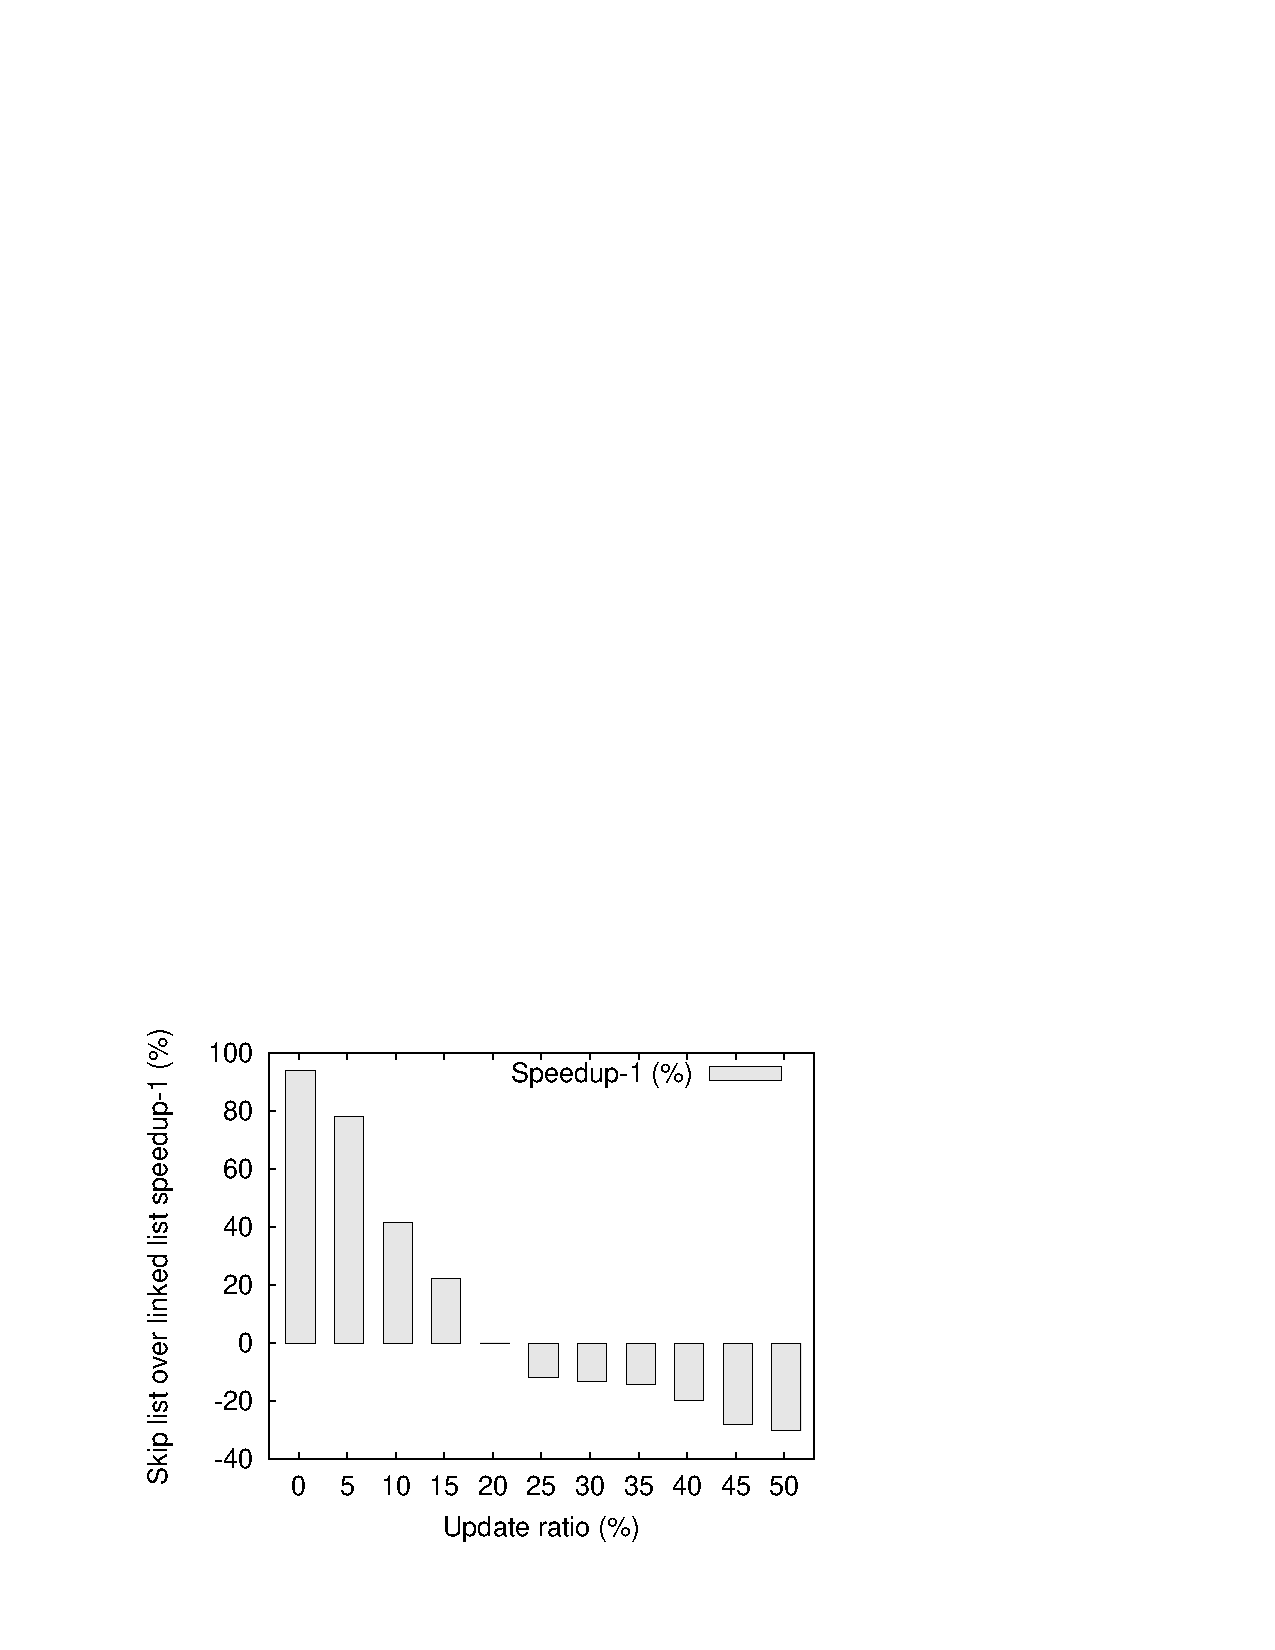
\includegraphics[scale=0.575,clip=true,viewport=50 50 400 300]{CF-general/fig/example}
	\caption{{\footnotesize Impact of contention on the performance of two 512-sized data structures (with 48 cores running with an increasing update ratio)\label{fig:contention}}}
\end{floatingfigure}

To better illustrate how contention can counterbalance the big-oh complexity  
in today's multi-/many-cores, Figure~\ref{fig:contention} depicts the performance
of a 48-core machine running the same set based experiment on a concurrent linked list, with $O(n)$ complexity,
and on a concurrent skip list, with $O(\log_2 n)$ complexity. 
A skip list, in short, is a structure that diminishes the complexity
of a linked list by being a sort of linked list 
%is a linked list 
whose nodes may have additional shortcuts pointing towards other nodes 
located further in the list~\cite{Pug90}. %(Skip lists are presented in Section~\ref{sec:sl}.)
%Figure~\ref{fig:contention} depicts the impact of contention on the performance of two integer set
%implementations, the first using a skip list offering a big-oh access complexity that is logrithmic in the 
%number of elements, the second using a linked list offering a linear access complexity.
In this experiment, 48 threads run insert/delete/contains accesses with an increasing proportion of 
update accesses over read-only ones on each of these two structures initialized with 512 
elements.\footnote{More precisely, this experiment was performed on a $4\times 12$-core AMD 
Opteron machine running at 2.1GHz and 32 GB of memory, each point is averaged 
over 5 runs of 5 seconds each, removes and inserts accesses are triggered with the same probability to keep the 
size expectation constant and removes/inserts that do not update the data structure are considered 
read-only accesses.}  To obtain the corresponding concurrent data structures used in the experiments, we simply encapsulated the 
sequential code of each access into an elastic transaction~\cite{FGG09}.
Interestingly, above 20\% updates the concurrent linked list is more efficient than the concurrent
skip list---this is shown by the negative values of the speedup-1. The reason is that the linked list 
updates are localized, that is, each of them only affects a constant number of nodes, typically the 
predecessor of the removed or of the newly inserted node. By contrast, the skip list updates 
may affect up to a logarithmic amount of predecessors for each removed of newly inserted node, 
producing additional contention.

This result is unsurprising as Herb Sutter noticed that linked list could better tolerate contention 
than balanced 
trees for similar reasons~\cite{Sut08}, yet it is interesting to observe experimentally that only 20\% 
updates make 
a linear complexity data structure better suited than a logarithmic complexity data structure on 
nowadays' multicore machines. 

In the light of the impact of contention on performance, we propose the \emph{Contention-Friendly (CF)}
methodology as a methodology to design new data structures that accommodate contention 
of modern multi-/many-core machines without relaxing the correctness of the abstractions.
To this end, we argue for a genuine decoupling of each access into an
eager abstract access and a lazy structural adaptation.
The abstract access consists in modifying the abstraction by minimizing the impact on the 
structure itself and aims at returning as soon as possible for the sake of responsiveness. 
The structural adaptation, which can be deferred until later, aims at adapting the structure to these changes by re-arranging elements or 
garbage collecting deleted ones.

We illustrate the CF methodology by designing three data structures with locks, universal primitives, and transactions: 
a skip list, a binary search tree and a hash table. 
As for the skip list, the aforementioned decoupling translates into splitting a 
node insertion into the insertion phase at the bottom level of a skip list and the structural 
adaptation responsible for updating pointers at its higher levels, or into splitting a node removal 
into a logical deletion marking phase and its physical removal and garbage collection.
Similarly, the decoupling of the binary tree accesses consists in inserting or logically removing a 
node prior to rebalancing and/or garbage collecting.
Finally, the hash table decoupling lies in inserting/deleting eagerly and resizing the structure lazily.

Our Java implementation of the resulting data structures indicates that our methodology leads to 
good performance on today's multicore machines. 
In particular using a micro benchmark, on a 64-way Niagara 2 machine our lock-based CF binary search tree improves 
the performance of the most recent Java lock-based binary 
search tree implementation~\cite{BCCO10} by up to $2.2\times$, our lock-based CF skip list 
improves the performance of Doug Lea's concurrent skip list adaptation of Harris and Michael algorithms~\cite{Har01,Mic02} by up to 
$1.3\times$, and our lock-free hash table outperforms by up to $1.2\times$ the JDK hash table, which is widely distributed in the $\lit{java.util.concurrent}$ package.
Finally, we show that state-of-the-art software transactional memories 
execute $1.5\times$ faster on average when the data structures are contention-friendly.

Section~\ref{sec:rw} describes the related work. Section~\ref{sec:cf} depicts the CF methodology, Section~\ref{sec:datastruct} illustrates it on three data structures. Section~\ref{sec:expe} presents the experimental results and Section~\ref{sec:conclusion} concludes. The companion appendix comprises the pseudo-code and correctness proofs of our CF algorithms, as well as additional experimentations using transaction-based variants of our CF algorithms and a discussion.

%
%\begin{abstract}
%In this paper, we propose a methodology to write speculation-friendly data structures.
%Although a lot of efforts were spent rethinking the transactional memory algorithms, 
%almost no efforts were spent rethinking the data structures accessed using transactions.
%
%Our methodology aims precisely at remedying this problem by listing the properties
%a data structure implementation should guarantee for speculative accesses to complete more rapidly.
%More specifically, this properties state that the same transactions should not comprise 
%abstract and structural modifications, that a structural modifications should be distributed 
%among sub-regions of the data structure, and that garbage collection should be acting 
%in the background independently from the actual logical removals.
%
%We illustrate this methodology with the first speculation-friendly library that comprises
%a binary search tree, a hash table, a linked list and a skip list.
%We show that this library outperforms the most efficient lock-based and lock-free alternatives 
%including the one of the Java concurrency package.
%Finally, we evaluate four state-of-the-art software TM libraries running on top of our library to show its portability.
%\end{abstract}
%
%\category{D.3.3}{Programming Languages}{Language Constructs and Features}[Concurrent programming structures]
%\category{E.1}{Data Structures}[Trees]
%\category{D.1.3}{Programming Techniques}{Concurrent Programming}[Parallel programming]
%\category{D.2.13}{Software Engineering}{Reusable Software}[Reusable libraries]
%
%\terms{Algorithms, Languages, Performance}
%
%\keywords{Abstract transaction, Structural transaction, Optimistic Concurrency, Transactional Memory}
%
%\section{Introduction}
%
%Multicore and manycore architectures are changing the way we write programs in three ways. 
%%{\bf Concurrency}
%First, every program, including irregular ones, should exploit concurrency thus all programmers must know how 
%to write a simple yet concurrent program.  
%%{\bf Contention Impact}  
%Second, the level of contention is expected to raise in irregular applications with the increasing number of 
%computational entities able to run concurrently, the cores, as they non-deterministically conflict when one process (thread) modifies a shared memory location another thread is accessing.
%%{\bf Resource Exploitation} 
%Third, the amount of cores at our disposal is expected to grow far beyond the traditional number of threads 
%we used to exploit, in part because reducing power consumption requires to simplify but multiply cores 
%
%To address the first challenge, speculative programming has proved effective in making concurrent programming modular~\cite{HHP05}: one can program a concurrent data structures another programmer can rely upon to simply derive her own 
%concurrent application.
%\vincent{What is speculation? Talk about Lampson's "Lazy and Speculative Execution in Computer Systems", Rachid's "Speculating Seriously", Idit's "Want scalable, speculate!", 
%Plan for the worst and optimize for the common: synchrony and low contention, but contention in many-core is expected to be quite high even at level of updates. Ravi Rajwar's thesis about multiprocessor speculation. Speculation for instructions, pipelining.}
%New programming constructs like transactions exploit this speculative approach~\cite{HM93,ST95}.
%Because transactions~\cite{HM93,ST95} cannot suffer from deadlocks, they encompass the drawback of trying to reuse
%lock-based data structures, and because they guarantee the atomicity of multiple accesses, they relieve the 
%programmer from the task of extending a library with hardware atomic primitives that apply to a single memory location.
%% transactions are appealing
%%New programming constructs like transactions have been suggested~\cite{HM93,ST95}.
%%Most transactions build upon \emph{optimistic synchronization}, 
%%where a sequence of shared accesses is executed speculatively and might abort.
%%They simplify concurrent programming for two reasons.
%The key concept of transactions is that the programmer only needs to delimit regions of sequential 
%code into transactions or to replace critical sections by transactions
%to obtain a safe concurrent program.
%%Second, the resulting transactional program is reusable by any programmer, 
%%hence a programmer composing operations from a transactional library into another 
%%transaction is guaranteed to obtain new deadlock-free operations that execute atomically.
%%By contrast, \emph{pessimistic synchronization}, where each access to some 
%%location $x$ blocks further accesses to $x$,
%%is harder to program with~\cite{PA11,RHW10} and hampers reusability.
%As a drawback of the simplicity of using transactions, 
%the existing transactional programs spanning from low level libraries to 
%topmost applications directly derive from program designed for non-speculative approach.
%
%\vincent{Cite Herb Sutter's Concurrency-friendly data structures.}
%We propose a speculation-friendly methodology to write highly efficient data structures 
%that reduce complexity of speculative accesses.
%This methodology generalizes the recent concepts of the speculation-friendly binary search 
%tree~\cite{CGR11} to arbitrary kind data structures to derive efficient libraries.
%Using this methodology, we propose four efficient data structures: a binary search tree, 
%a hash table, a linked list and a skip list.
%We show that a Java adaptation of our speculation-friendly binary search tree~\cite{CGR11} is more efficient 
%than the most recent concurrent tree alternative~\cite{}.
%In particular it is also more efficient than the $\lit{ConcurrentSkipList}$ from the Java concurrency package.
%More interestingly, we show that our new speculation-friendly skip list algorithm is even more efficient than 
%all these former algorithms. Besides being the most efficient logarithmic-complexity data structure known in Java 
%to date, it confirms that the speculation-friendly methodology is a powerful concept to obtain very efficient 
%data structures.
%
%The speculation-friendly methodology overcomes the two remaining modern challenges posed by the 
%multicore era.
%First, it limits contention by relaxing the existing data structure invariants without annihilating the abstraction semantics. Previous work on relaxing data structure invariants tends to weaken the semantics of the abstraction.
%For example, the Intel\textregistered{} Threading Building Blocks (TBB)\footnote{http://threadingbuildingblocks.org} relaxed the FIFO policy of the queue with multiple consumers/producers. Recent proposals~\cite{Sha11} tend to trade similar guarantees to obtain highly concurrent stacks.
%
%% problem
%The problem of adapting data structures for speculative execution remains vastly unexplored 
%though our recently published binary search tree~\cite{CGR12} clearly motivates the importance of such a topic.
%Pessimistic operations must typically guarantee some invariants about the location of nodes in 
%the structure. These invariants help ensure that the complexity of
%searching a given element is always upper-bounded, guaranteeing the step complexity.
%To preserve these invariants,
%an operation affecting the structure by removing, inserting or simply moving nodes
%must additionally check whether its modification affects the invariants. If so, it must then execute a dedicated \emph{restructuring}, 
%a process that modifies the data structure without modifying the state of the abstraction it implements, to compensate the modification 
%and preserve the invariants.
%The modification and its compensating restructuring must naturally appear to be executed \emph{atomically}, 
%in a single indivisible step from the standpoint of the system, to make sure the transient invariant violation 
%is not visible from further operations.
%
%
%However, the resulting complexity really depends on the type of synchronization.
%The complexity of pessimistic concurrency control is tied to the number
%of protected steps that are guaranteed to complete despite blocked 
%attempts of interfering, whereas the complexity in optimistic concurrency 
%control is tied to the number of speculative attempts that fail due to 
%unavoidable interferences.
%Put simply, while a pessimistic update on a data structure 
%tries to minimize the number of its successful protected steps, the 
%optimistic one should rather minimize its unsuccessful speculative steps.
%
%% state of the art
%Currently, three techniques exist to boost the performance of the transactions used to access 
%data structures.
%%Currently, three major research directions are explored to  
%%obtain efficient transactional executions on data structures.
%First, high-level conflict detection aims at ignoring the low-level 
%conflicts of structural transactions by using abstract 
%locks~\cite{Mos06,NMA+07,CMC07,HK08,ALS09}.
%Second, various language extensions have been
%proposed as escape mechanisms within a transaction 
%to limit the transaction bookkeeping~\cite{HLMS03,CH05,FGG09,AMT10}. 
%The former approach exploits the application semantics and cannot 
%be automated while the latter approach requires the programmer
%to tune the underlying TM implementation generally not supported 
%by TM compilers~\cite{abi}. 
%Third, the combination of various transaction semantics cope with unsupported
%language extensions~\cite{FGG09,GG11} but still puts the burden of choosing the 
%right semantics on the programmer.
%The idea of boosting the speculatively accessed data structure itself has just been suggested
%but we only evaluated binary search trees~\cite{CGR11} and ignore whether it can be applied to other
%data structures. 
%
%% contributions
%We propose a methodology to write \emph{speculation-friendly data structures}. In short, it consists in relaxing transiently their structural invariants without hampering the abstraction consistency in order to speed up transaction-based accesses.  
%We illustrate this methodology through a speculation-friendly library that comprises four data structures:
%a binary search tree, a hash table, a linked list and a skip list. The characteristics of these new algorithms 
%are as follows:
%\begin{itemize}
%	\item {\bf Binary search tree.}
%We verify that our previous binary search tree~\cite{CGR12} respects the methodology.
%In particular we implemented an object-based version in Java of our previous C implementation to evaluate
%its performance against the performance of the latest (after ours) binary search tree algorithm~\cite{BCCO10}. We show that our resulting algorithm is \vincent{TODO}$\times$ faster than the most recent tree algorithm, and \vincent{TODO}$\times$ faster than the skip list  $\lit{java.util.concurrent}$ package (the only propose data structure with logarithmic access complexity).
%	\item {\bf Linked list.}
%We propose a new linked list algorithm that is speculation-friendly in that is decouples the logical and physical 
%removal process 
%As linked list data structures have the appealing aspects of supporting localized updates, its performance benefit is marginal compared to other data structures. \vincent{Maybe compare against synchronizedSet Linked List?}
%	\item {\bf Hash table.} 
%We propose a new hash table algorithm that is speculation-friendly in that its resize operation is done in the background rather than being part of an update operation that exceeds the maximal tolerated load.
%In addition, we reuse our speculation-friendly linked list algorithm to implement each independent bucket.
%	\item {\bf Skip list.}
%We propose a new skip list algorithm that is speculation-friendly in that the structural level of each node are adapted in the background rather than being tightly coupled with the corresponding insert operation.
%We compare our skip list performance against the $\lit{java.util.concurrent}$ skip list and our speculation-friendly tree algorithm. Perhaps surprisingly, this data structure is the most efficient data structure we have observed.
%\end{itemize}
%Finally, we also evaluate a version of the speculation-friendly library as part of the bytecode instrumentation 
%framework Deuce~\cite{KSF10}. Although this framework adds a significant overhead to the execution time, it greatly 
%simplifies the usage of various transactional memory algorithm. We report on the performance of 
%TL2~\cite{DSS06}, LSA~\cite{RFF06}, ${\mathcal E}$-STM~\cite{FGG09},  NOrec~\cite{DSS10} when running 
%speculation-friendly data structure and in particular we illustrate the 
%portability of our library to TM systems satisfying the standard TM interface~\cite{abi}.
%
%%Ok, for the tree we should keep in mind that:
%%- the background rotating thread was originally proposed by Mander and Ladner in 1984 
%%- the distributed rotation (w/ propagation) was proposed by Bouge et al. in 1998
%%- the separate garbage collector was proposed by Dijkstra et al. in 1978
%%But the novelty is to decouple *speculative* operations.

\section{Related Work}\label{sec:rw}

Various complexity metrics exist to evaluate data structures efficiency on a given workloads. 
% big-oh notation in theory
From a theoretical point of view, the big-oh notation helps to derive data structures whose access step 
complexity is proportional to the total number of elements.
Typically, balanced trees have a logarithmic big-oh access complexity whereas non-overloaded hash 
tables have a constant big-oh access complexity.
This big-oh complexity does not capture the cost of contention and theoretical models have been 
explored to remedy this issue~\cite{DHW97}. Unfortunately, there are not enough evaluations of this 
impact in practice. 

% locality in practice
From a more pragmatic point of view, the locality of data both in terms of space (i.e., the promiscuity of 
data stored in memory) and time (i.e., 
the closeness of the points in time at which they are accesses) has been an important metric of 
consideration when implementing data structures in cache-coherent systems.
Cache-aware and cache-oblivious data structures try to exploit locality to maximize the chance of cache 
hits. While the former data structures rely on some tunable parameter that can accommodate the 
targeted platform like the Judy array\footnote{\texttt{http://judy.sourceforge.net}}, the later aims at being 
more portable by flattening cleverly structural nodes into memory~\cite{FLPR99}, for example the tree algorithm 
of van Emde Boas et al.~\cite{vEKZ76}. Both approaches are tied to cache-coherent machines but do 
not accommodate upcoming many-core platforms whose cache-coherence is either 
limited~\cite{WGH+07} or absent~\cite{MRL+10}. 
%In particular, this observation led researchers to 
%rethink even existing shared-memory cache-coherent machines in terms of distributed systems, where threads communicate by sending inter-core messages instead 
%of assuming a simplifying but costly shared memory~\cite{BBD+09}.

The decoupling of the update and rebalancing was vastly explored in the context 
of trees~\cite{GS78,Kes83,NSW87,NS98,UR84,IRISAppr,Bal06,CGR12} 
%Various database trees where proposed with a decoupling of update and 
%rebalancing~\citep{GS78,Kes83,NSW87,NS98,UR84,IRISAppr} 
but this idea was 
not generalized to other search structures.
The decoupling of the removals in logical and physical phases was originally studied in transactional systems~\cite{Moh90}
and later applied to various lock-free data structures including linked lists~\cite{Har01}, hash tables~\cite{Mic02}, skip lists~\cite{Fra03,FR04} and binary search trees~\cite{EFRB10}
but insertions in these data structures were not decoupled.
The contention friendly methodology generalizes these decoupling into an eager abstract access and a lazy structural adaptation that benefit
both insertions and removals.

Our methodology is independent from the synchronization primitive used but lies essentially in splitting 
accesses into an eager abstract access and a lazy structural adaptation.
Although we focus essentially on lock-based data structures, we also evaluate the benefit of various
transactional memory algorithms when running our contention-friendly data structures.
We have already illustrated the benefit of decoupling accesses into separate transactions 
in~\cite{CGR12} on a C-based 
binary search tree.  In such optimistic executions, this decoupling translated into avoiding a conflict with a 
rotation from rolling back the preceding insertion/removal.
Here we generalize our previous work by showing how a similar decoupling can benefit 
pessimistic execution and various search structures and we compare our results to existing Java concurrent structures.
%We generalize our previous work to pessimistic executions and by experimenting our methodology on several Java-based STM algorithms 
%and additional contention-friendly data structures.
Previous investigations on improving the performance of transaction-based data structures focused 
exclusively on the improvement of the transaction algorithm. Some of these investigations led to the 
development of novel transaction models based on abstract locks to ignore low level conflicts~\cite{NMA+07,HK08}, 
or elastic transactions~\cite{FGG09}.

Finally, Shavit suggests to relax data structure guarantees in the light of the new multicore context~\cite{Sha11}. A stack algorithm and several relaxations to this algorithm
are presented to support concurrency. The objective as well as the means to achieve it are quite different from ours. 
First, the problem raised by placing the stack into the multicore context is that performance drops below the sequential stack performance, and 
the goal is to diminish contention to limit this concurrency drawback. By contrast, we focus on deriving alternative data structures that are more scalable than highly concurrent ones, hence leveraging multi-/many-cores.
Second, the goal of limiting contention induced by multiple cores is achieved by relaxing consistency. In the stack example, this relaxation boils down 
to replacing linearizability by quiescent consistency, guaranteeing that the last-in-first-out policy of an access is only with respect to preceding calls 
when no other accesses execute concurrently.
Conversely, the contention friendly methodology aims at replacing existing data structures without relaxing their abstraction consistency: all accesses remain linearizable.

%\vincent{We should talk about the java.util.concurrent package that some decoupling with lazy techniques. At least explain the difference with concurrentHashMap and ConcurrentSkipListMap/Set.}

\section{The CF Methodology at a Glance}\label{sec:cf}

%The Contention-Friendly (CF) Methodology relies on several observations on speculative execution: (i)~multicore raises contention that impacts sometimes more the execution complexity than the structure itself; (ii)~multi/many-cores provide more computational resources than we used to exploit.
In this section, we give an overview of the Contention-Friendly (CF) methodology by describing how to write contention-friendly data structures.

The CF methodology aims at modifying the implementation of existing data structures using two simple rules without relaxing their correctness. The correctness criterion ensured here is linearizability~\cite{HW90}.  The data structures considered are \emph{search 
structures} because they organize a set of items referred to as \emph{elements} in a way that allows to retrieve the unique expected position of an element given its value. 
The typical abstraction implemented by such structures is a collection of elements that can be specialized into various sub-abstractions like a set (without duplicates) or a dictionary (that maps each element to some value). We consider \emph{insert}, \emph{delete} and \emph{contains} operations 
that respectively inserts a new node associated to a given value, removes the node associated to a given value or leaves the structure unchanged if no such node is present, and returns the node associated to a given value or $\bot$ if such a node is absent. Both inserts and deletes are considered \emph{updates}, even though they may not modify the structure.

\begin{table*}
\begin{center}
{\footnotesize
\renewcommand{\tabcolsep}{1pt}
\renewcommand{\arraystretch}{1}
\begin{tabular}{|l|l|l|l|}%{|l|l|rl|}
  \hline
  {\bf Data structure} & {\bf Invariant} & {\bf Abstract modifications} & {\bf Structural adaptations} \\ \hline\hline

  {\bf Hash tables} & constant load factor & key-value pair insertion & adding buckets and rehashing \\
  & (i.e., $\#\lit{nodes} / \#\lit{buckets} = O(1)$) & logical deletion & physical deletion + rehashing\\ \hline
  %{\bf Linked lists} & linear access time complexity (i.e., $O(n)$)& logical deletion & physical deletion \\ \hline
    {\bf Search trees} & balance & node insertion & rotation \\
  & (i.e., shortest route to leaf $\approxeq$ longest route to leaf) & logical deletion & physical deletion + rotation \\ \hline
  {\bf Skip lists} & node distribution per level & horizontal insertion & vertical insertion + increasing toplevel \\
  & (i.e., $\Pr[\ms{level}_i=j] = 2^{O(j)}$) & logical deletion & physical removal + decreasing toplevel \\ \hline
\end{tabular}}
\end{center}
\vspace{-1.5em}
\caption{\footnotesize Decoupling example of existing data structure accesses into an abstract modification and a structural adaptation\label{table:restructuring}}
\end{table*}
%\vspace{-1em}

%The first rule 
The key rule of the methodology is to decouple each update into an \emph{eager abstract modification} and a \emph{lazy structural adaptation}. The secondary rule is to make the removal of 
nodes selective and tentatively affect the less loaded nodes of the data structure.
These rules induce 
%This requires 
slight changes to the original data structures as summarized in Table~\ref{table:restructuring}, that result in a corresponding 
data structure that we denote using the \emph{contention-friendly} adjective to differentiate them 
from their original counterpart.

\vspace{-1em}
\subsection{Eager abstract modification}

Existing search structures rely on strict invariants (cf. Table~\ref{table:restructuring}) to guarantee their big-oh complexity, hence each 
time the structure gets updated,  the invariant is checked and the structure is accordingly 
adapted instantaneously. While the update may affect a small sub-part of the abstraction, 
its associated restructuring is a global modification that conflict potentially with any concurrent update, 
thus increasing contention.
 
The CF methodology aims at minimizing such contention by returning eagerly the modifications of the 
update operation that makes the changes to the abstraction visible. By returning eagerly, each 
individual process can move on to the next operation prior to adapting the structure. It is noteworthy 
that executing multiple abstract modifications without adapting the structure does no longer guarantee the big-oh step complexity of the accesses, yet such complexity may not be the predominant factor in 
contended execution as we reported in the Introduction.

A second advantage is that removing the structural adaption from the abstract modification makes the cost of each operation more predictable.  All operations share similar cost and create the same amount of contention.
%whereas
%in existing data structures for example one insert in a tree might require $O(\log(n))$ rotations while 
%another
%insert might not require any rotation, leading to unpredictable response time.
More importantly the completion of the abstract operation does not depend on the structural adaptation
(like they do in existing algorithms) 
so the structural adaptation can be performed differently, using and depending on global information.
%This means that the adaptations can be preformed differently without directly impacting the abstract operations.
%For example the modifications can use global information or be more costly than they are in existing algorithms

\vspace{-1em}
\paragraph{The skip list example.}

A traditional skip list picks a level for each node when they are
inserted based on some pseudo-random function.  The aim of this function
is to distribute the levels so that operations have an average cost of
$O(\log{n})$.  In certain workloads this can be preferred over trees due
to the assumption that rotations are more costly. 
When a node is inserted in
the contention-friendly skip list it has a level of one, which is all that is needed to ensure the correctness of the abstraction.

\begin{floatingfigure}{7.5cm}
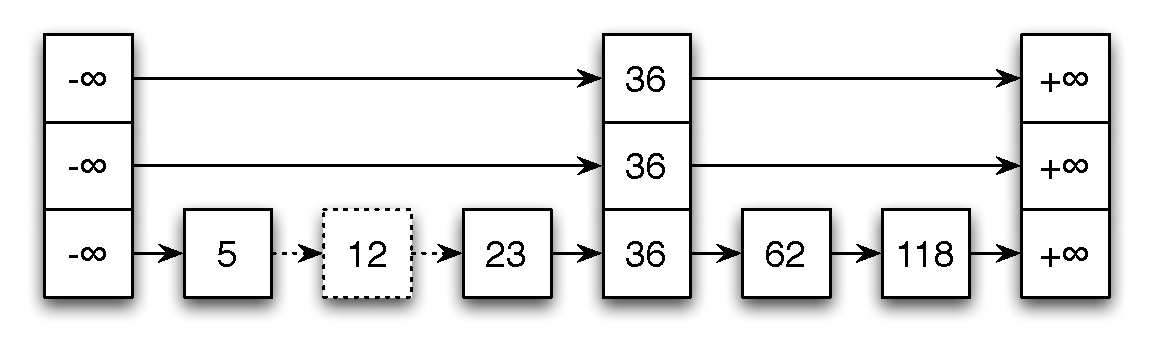
\includegraphics[scale=0.35]{CF-general/fig/horizontal-insert}
%\vspace{-1em}
\caption{\footnotesize{Inserting horizontally in the skip list\label{sfig:horizontal}}}
\end{floatingfigure}

As an example, assume we aim at inserting an element with value 12 in a skip list.  Our 
insertion consists in an abstract modification that updates only the bottom most level by inserting the new 
node as if its level was the lowest one leading to Figure~\ref{sfig:horizontal} where dashed arrows indicate the freshly modified pointers.
We defer the process of linking this same node at higher levels, to diminish 
the probability of having this insertion conflict with a traversing operation.

\subsection{Lazy structural adaptation}

The purpose of decoupling the structural adaptation from the preceding abstract modification is to enable its postponing (by, for example, dedicating a separate thread to this task), hence the term ``lazy'' structural adaptation.
The main intuition here is that this structural adaptation is intend to ensure the big-oh complexity rater 
than to ensure correctness of the state of the abstraction.
Hence, the linearization point belongs to the execution of the abstract modification and not the structural 
adaptation and postponing the structural adaptation does not change the effectiveness of operations.
The visible modification applied to the abstraction (and the structure) during the abstract modification guarantees that any further operation applying to the same structure will observe the changes. This helps ensuring that all operations are linearizable in that real-time precedence is 
satisfied. In Appendix~\ref{sec:proof} we show that our structures implement a linearizable abstraction. 

This postponing has several advantages whose prominent one is to enable merging of multiple
adaptations in one simplified step. Although the structural adaptation might be executed in a 
distributed fashion, by each individual updater threads, one can consider centralizing it at one 
dedicated thread.
Since these data structures are designed for architectures that use many cores
performing the structural adaptation on a dedicated single separate thread, takes advantage of 
hardware that might otherwise be left idle.
Only one adaptation might be necessary for several abstract modifications and minimizing the 
number of 
adaptations decreases accordingly the induced contention. Furthermore, several adaptations can 
compensate each other as two restructuring can lead to identity. For example, a left rotation executing 
before a right rotation at the same node may lead back to the initial state and executing the left rotation 
lazily makes it possible to identify that executing these rotations is useless.

\paragraph{The skip list example.}

As explained in the previous example the insertion executes in two steps. Once the horizontal 
insertion of node 12, depicted in Figure~\ref{sfig:horizontal}, is complete, a restructuring is necessary to 
ensure the logarithmic  complexity of further accesses. 
\begin{floatingfigure}{7.5cm}
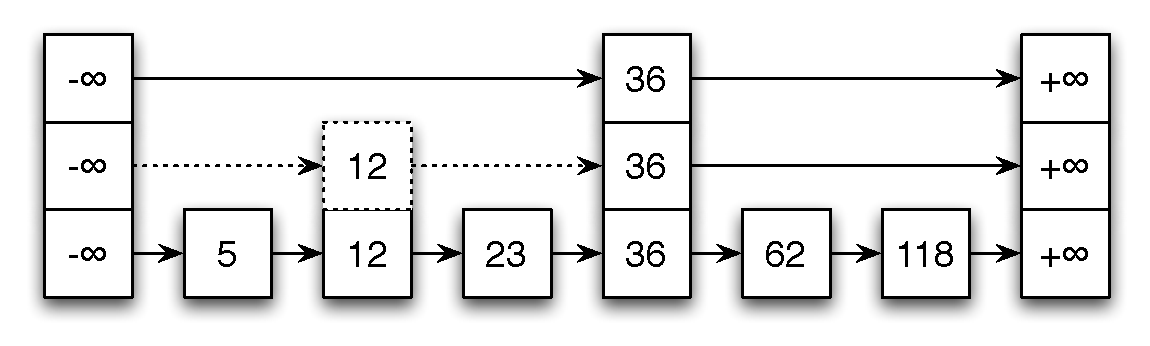
\includegraphics[scale=0.35]{CF-general/fig/vertical-insert}
%\vspace{-1em}
\caption{\footnotesize{Adapting vertically the skip list structure\label{sfig:vertical}}}
\end{floatingfigure}

A separate structural adaptation step is accordingly raised to increase the node level appropriately.
%In a tree the physical insertion is decoupled from any necessary rotations.
%In a hash table insertion is decoupled from any resizing and rehashing operations.
The insertion at higher levels of the skip list is executed as a separate step, which guarantees 
eventually a good distribution of nodes among levels as depicted in Figure~\ref{sfig:vertical}.
This decoupling allows higher concurrency by splitting one atomic operation into two atomic operations.

\subsection{Selective removal}
In addition to decoupling level adjustments, we do selective removals.
A node that is deleted is not removed instantaneously, instead it is
marked as deleted.  The structural adaptation then selects cleverly nodes that
are suitable for removal, i.e., whose removal would not induce high contention.
This is
important because removals may be expensive.  
Removing a frequently accessed node
requires locking or invalidating a larger
portion of the structure.
%In the worst case this node would be the root of a tree or the tallest
%node in a skip list.
Removing such a node is likely to cause much more contention
than removing a less frequently accessed one.
In order to prevent this, only nodes
that are marked as deleted and have a level of 1 (in the skip list) or 
a single or no children (in the tree) are removed.
This leads to less contention, but also means that certain nodes that are marked as deleted will not be removed.
In the tree it has already been observed that only removing such nodes~\cite{CGR12},\cite{BCCO10} results in a similar sized structure
as existing algorithms.
In the skip list the level of a node is calculated in such a way that after a structural adaptation is performed less than
half the nodes (in the worst case) in the list will be marked as deleted.
In practice this number is observed to be much smaller.

\paragraph{The skip list example.}
Let us look at a specific example with the skip list.
On the one hand, a removal of a node with a high level, say the one with value 36 in 
Figure~\ref{sfig:vertical}, would typically induce more contention than the removal of a node with a lower 
level, say the one with value 62 spanning a single level.
The reason is twofold. First removing a node spanning $\ell$ levels boils down to updating $\ell$ 
pointers which increase the probability of conflict with a concurrent operation accessing the same 
pointers, hence removing node with value 36 requires to update 3 pointers while node with value 63 
requires to update a single pointer. Second, the organization of the skip list implies that higher level 
pointers are more likely accessed by any operation, hence the removal of 36 
typically conflicts with every operation concurrently traversing this structure (because all these 
operations would follow the topmost left pointer) whereas the single next pointer of 62 is unlikely accessed by concurrent traversals.
Removing a tall node such as 36 would also mean that in order to keep the logarithmic complexity of the traversals a
node would have to take its place at an equivalent height.

%\vincent{Talk about distribruted vs. centralized restructuring}
%The final advantage is thanks to the multicore hardware.
%Even though the structural adaption is done separately, someone stills need to do them so that the abstract operations remain efficient.
%Since these data structures are designed for architectures that use many cores the structural adaptations are performed entirely by a separate thread,
%taking advantage of hardware that might otherwise be left idle.

\subsection{Avoiding contention during traversal}
Each abstract operation ($\ms{contains}$, $\ms{insert}$, $\ms{delete}$) of a tree or a skip list is %not so different from in an existing sequential algorithm.
%They are each
expected to traverse $O(\log{n})$ nodes.
Given that the traversal is the longest part of the operation, the CF algorithms try to avoid as often as possible producing contention.
%
Concurrent data structures often require more complex synchronization operations during traversal (not including the updates done after the traversal).
% Such as
For example, locking nodes in a tree helps ensure that the traversal remains on track during a concurrent rotation~\cite{BCCO10}, using $\lit{compare-and-swap}$ operations during traversal helps the raising and lowering of levels of a concurrent $\ms{insert/delete}$ in a lock-free skip list~\cite{Fra03}, or using optimistic strategy helps at the risk of having to restart~\cite{HLL07,HS08}.

Usually these synchronization operations are required due to structural adaptations and the CF 
algorithms structural adapt differently to especially so that operations can avoid using
locks or synchronization operations during traversal.
%
\remove{
The structural adaptations are also designed to avoid contention where possible.
This means applying the selective removal of nodes that are traversed less 
frequently, as well as using locks/synchronization as little
and as localized as possible. For example, only reads/writes are used when modifying the upper levels of the CF skip list, rotations in the CF tree are performed as localized
operations, and rehashing of the CF hash table is done per bucket.
}

\section{Putting the CF Methodology to Work}\label{sec:datastruct}

Here we present how we apply the contention-friendly (CF) methodology to three data structures. For further detail on the algorithms and correctness proofs please refer to Appendix~\ref{app:pseudocode}
and Appendix~\ref{sec:proof}, respectively.


%\subsection{CF Tree and Skip list}

\subsection{CF Skip list}

The CF skip list is made up of several levels of linked lists,
with the bottom level being a doubly linked list.
Each node on the bottom level contains the following fields:
A key $k$, a $\ms{next}$ and $\ms{prev}$ node pointers, a lock field, a $\ms{del}$ flag indicating 
if the node has
been marked deleted, and a $\ms{rem}$ flag indicating if the node has been physically removed.
The algorithm presented here is lock-based, however, we have derived a transaction-based version
(cf. Appendix~\ref{sec:tm}).
% relaxing structural invariants
%As the complexity of speculative execution does not only depend on the distribution of levels of the skip 
%list nodes but also on the contention, we aim at minimizing both instead of focusing on the ideal 
%distribution. Specifically, we trade transiently the ideal distribution of levels to diminish 
%contention of speculative accesses by avoiding updating the higher levels as part of the update 
%operation.
%
%Transactionalizing a skip list implementation, be it sequential with no 
%synchronization technique or concurrent using locks for synchronization purpose, would naively result 
%in encapsulating each update operation into a dedicated transaction, yet this update would  typically do several things.

%\begin{figure}[ht!]
%\begin{center}
%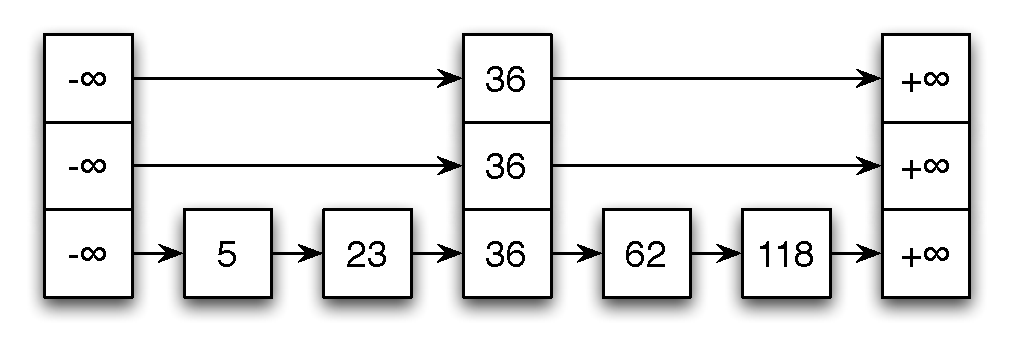
\includegraphics[scale=0.45]{fig/skiplist}
%\caption{A skip list example where removing node 62 induces more contention than removing node 36\label{fig:sl-remove}}
%\end{center}
%\end{figure}


\remove{
On the other hand, an insertion operation, say of value 12 with no loss of generality, as depicted in Figure~\ref{fig:sl-insert} would typically insert \emph{horizontally} a new node at the bottom level of the skip list 
(Figure~\ref{sfig:horizontal}) but also update \emph{vertically} the higher levels to 
guarantee that further operations have a logarithmic complexity (Figure~\ref{sfig:vertical}). 
The horizontal phase is both a structural and an abstraction modification: once executed the 
state of the abstraction reflects the changes. By contrast, the vertical phase is only a structural 
adaptation that does not impact the state of the abstraction.
% rewording
In other words, inserting the node at the bottom level guarantees that the node is 
reachable and that the value is part of the abstraction. Updating the higher 
levels is only necessary for efficiency purpose, not for safety purpose. 
}

\remove{
Motivated by the fact, that future multicore will provide more and more cores, we 
aim at exploiting additional cores (at least one) responsible of maintaining the 
data structure in the background.
}
\paragraph{Abstract operations.}
The goal of these CF algorithms is for the abstract operations
 to encounter and produce as little contention as possible.
%
In particular, it boils down to 
%As previously discussed this means deletions are done by 
setting the nodes
$\ms{del}$ flag to $\lit{true}$ to delete a node 
as well as linking 
%insertions only insert 
a new node to the bottom list level to insert it.
These modifications are necessary to guarantee that
linearizability, with all other structural adaptations being saved for later execution.
For the sake of safety, the abstract insertion acquires a lock on the predecessor 
node of the to-be-inserted node whereas the abstract deletion acquires a lock 
on the to-be-marked node. The lock is immediately released after the insertion 
or deletion completes. 
%In order to ensure
%these operations are able to execute safely they lock the node they modify.
%For the insert this is the node previous to where the new node will be inserted
%and for the delete this is the node that will be marked as deleted.

No locks are acquired during the traversal, inducing no contention.
%In order to avoid contention during traversal,  no locks are acquired.
More precisely, while traversing upper levels the operation will move forward in the list using
the $\ms{next}$ pointer until it encounters a node with a larger key than the one being search for
at which point it will move down a level, similarly to a bare sequential implementation would do.
At the bottom level the traversal may end up on a node that is physically removed due
to a concurrent structural adaptation $\ms{remove}$ operation, in this case it travels backwards in the list
following the $\ms{prev}$ pointer until it arrives at a node that has not yet been removed.
%by updating as many pointers as its level. By contrast, a removal of node with a lower level, say the one with value 63 in Figure~\ref{fig:sl-insert} spanning a single level, would simply require to update a single pointer. 

\paragraph{Structural adaptation.}

The first task of the structural adaptation is to remove nodes marked as deleted
who have a height of $1$.
In order to prevent conflicts with concurrent abstract operations
the node $\ms{n}$ to be removed and its predecessor in the list ($\ms{n.prev}$) are locked.
The prior nodes $\ms{next}$ pointer ($\ms{n.prev.next}$) is then modified so that it points to the next 
node ($\ms{n.next}$), and the next node's $\ms{prev}$ pointer ($\ms{n.next.prev}$) is then modified to point to the previous node ($\ms{n.prev}$).
Finally the $\ms{n}$'s $rem$ flag is set to true and the locks are released.

The structural adaptation must also modify the level of nodes in order to ensure
the $O(\log{n})$ expected traversal time.
Since neither removals nor insertions are done as they are in traditional skip lists,
calculating the height of a node must also be achieved differently.
Existing algorithms call a random function to calculate the heights of nodes, but
if this same function was used here the structure would end up with
excessive tall nodes.

When choosing the heights it is important to consider that
the fundamental structure of a skip list is not designed
to be perfectly balanced but rather probabilistically balanced.  
Consider a perfectly balanced skip list.  The node in the very middle of the list would
be the tallest node and the nodes just to the right and left of this
node would be nodes with height $1$.  Now if a couple new nodes are
inserted at the very end of the list then to
re-balance the skip list the node that was previously the tallest
node would now be shrunk to a level of $1$, and one of its
neighboring nodes which previously had height of $1$ would become the tallest node.
Instead a scheme of approximately balanced is more fitting for the skip list
(as this is what the existing algorithm's random functions do).

By contrast, the CF skip list deterministically adjusts the level of nodes.
%The contention friendly algorithm uses the following
%procedure to adjust the heights of the nodes.
From the bottom level going upwards, it traverses the entire list of the level, 
and each time it observes that 3 consecutive nodes whose height equals this level,
it raises the level of the second of this node (the one in the middle) by 1.
%Starting from the bottom level going upwards, do the following at
%each level:
%Traverse the entire level.
%Each time $3$ nodes in a row of height equal to the current level
%are encountered, raise the level of the middle of these nodes by $1$.
Such a technique approximates the targeted number of nodes present at each level, 
balancing the structure.
%This creates an approximate correct number of nodes at each level
%and creates an approximately correct balance.
Doing this is similar to the original intuition of the skip list, there is no
frequent re-balancing going on, tall nodes will stay tall nodes.
Less modification of the taller nodes also means less contention
at the frequently traversed locations of the structure.

Given that the number of nodes in the list might also shrink
the height of nodes might also be lowered.
When the height of the tallest node is greater than some threshold
(usually when the height is greater than the $\log$ of the total number of
nodes in the list) the entire bottom index level of the skip list is simply removed
by modifying the $\ms{down}$ pointers of the level above.
Doing this avoids constant modification of the taller nodes and ensures
there are not too many marked deleted nodes left in the list.

\subsection{CF Tree}

The CF tree is a binary search tree. Each of its nodes contains the following fields: a key $\ms{k}$, pointers $\ms{l}$ and $\ms{r}$ to the left and right children nodes, a lock field, a $\ms{del}$ flag indicating if the node has
been marked deleted, and a $\ms{rem}$ flag indicating if the node has been physically removed.
As for the CF skip list, the CF tree algorithm presented here is lock-based but we also derived 
a transaction-based variant of it.

\paragraph{Abstract operations.}
Similarly to the CF skip list operations the 
$\ms{insert}$ and $\ms{delete}$ operations must acquire a lock on the node
they modify.
A $\ms{delete}$ operation sets the node's $\ms{del}$ flag to $\lit{true}$ while an $\ms{insert}$ operation allocates a new node and modifies the parent's child pointer to point to it.

The traversal is performed without locks.
At each node the traversal travels to the right child if the node's key is larger than $k$,
otherwise it travels to the left child.
Since locks are not used, the traversal might get caught during a concurrent removal or rotation, but
the structural adaptation is done in such a way that
the traversal can continue safely following the child pointers.

\paragraph{Structural adaptation.}
The structural adaptation is in charge of removing marked deleted nodes that have
at most one non-$\bot$ child pointer.
Removals are done by first locking the node $n$ to be deleted and its parent.
The parent's child pointer is then modified so that it points to $n$'s non-$\bot$
child (if any).
Next $n$'s child pointers are modified so that they point upwards to it's parent node
allowing concurrent traversal that arrived on this node a safe path back to the tree.
Finally $n$'s $\ms{rem}$ flag is set to $\lit{true}$ and the locks are released.

The structural adaptation must also perform rotations in order to ensure the tree is balanced
so that traversal can be done in $O(\log{n})$ time.
Methods for performing localized rotation operations in the binary trees have already been examined and proposed
in several works such as ~\cite{CGR12,BCCO10}.
The main concept used here is to propagate the balance information from a leaf to the root.
A leaf is known to have height of $0$ for their left and right children.
This information is then propagated upwards by sending the height of the child to the parent where the value
is then increased by $1$.
Local rotations are performed depending on this information and result eventually in a balanced tree.

In order to avoid using locks and aborts/rollbacks during traversals, rotations are performed differently than traditional rotations.
Before performing the rotation the parent node and its child node that will be rotated are locked in order to
prevent conflicts with concurrent $\ms{insert}$ and $\ms{delete}$ operations.
In a traditional rotation there is one node $\ms{n}$ that is rotated downwards and one node (one of $\ms{n}$'s children)
that is rotated upwards.
A traversal preempted on the node rotated downwards ($\ms{n}$ in this case) is then in danger of being set off track and missing the
node it is searching for.
The rotations performed in the CF algorithm avoid this by not actually rotating $\ms{n}$ at all,
meaning that after the rotation $\ms{n}$ still has a pointer to the node that is rotated upwards allowing traversals to continue safely.
Instead a new node takes $\ms{n}$ place in the structure.
This new node is set to have the same values and pointers as $\ms{n}$ would if a rotation was performed as normal.
After the rotation, the node $\ms{n}$ has its $\ms{rem}$ flag set to $\lit{true}$ 
%as it is no longer in the tree.
and, finally, the locks are released.

\remove{
The main difference between the algorithm presented here is the decoupling of these operations.
The second difference is a slightly more complicated rotation procedure is used here
(but since they are performed separately, they do not slow the abstract operations).
This modified rotation procedure allows concurrent traversals to pass rotated nodes without having to use
synchronization methods.
A description of the rotations can be found in section \cite{sec:treemaint}.
}

\subsection{CF Hash table}

The CF hash table contains an array of pointers with each location pointing to $\bot$ or to
a list of nodes. Each node contains the following fields.
A key $\ms{k}$, and a $\ms{next}$ pointer pointing to the next node in the list.
This algorithm is lock-free (relying on $\lit{compare-and-swap}$ for synchronization) but we derived a transaction-based variant of it (cf. Appendix~\ref{sec:tm}).

\paragraph{Abstract operations.}

Given that the traversal for the $\ms{contains}$, $\ms{insert}$, $\ms{delete}$ operations has complexity $O(1)$ and not $O(\log{n})$ the
hash table operations are performed slightly differently.
In fact, the shortness of the hash table operations brings two main differences to the algorithm.

First physical removals are done from within the $\ms{delete}$ operation.
This is because the contention caused by removing the node will only be with other nodes of that bucket which are expected to be
$O(1)$.

Second the algorithm is made lock-free because given the short operations, a cache miss caused 
by loading a lock could be relatively costly.
Other implementations might avoid this by using coarser grained locks, like lock-striping, but
this can cause contention on the lock(s).
Instead we use a lock-free implementation where each operation only uses (at most)
a single synchronization operation, which is a $\lit{compare-and-swap}$ on the given bucket pointer.

For the sake of linearizability of operations the $\lit{compare-and-swap}$ always happens
at the same location (on the bucket pointer) and the $\ms{next}$ pointer of list elements
is never modified after node creation.
An $\ms{insert}$ will $\lit{compare-and-swap}$ a new node as the first element of the list, while
a $\ms{delete}$ will remove a node by creating a new list that does not contain the node
and $\lit{compare-and-swap}$ this new list to the bucket.
If the $\lit{compare-and-swap}$ fails due to a concurrent operation
then the operation retries from the beginning.

\paragraph{Structural adaptation.}

The structural adaptation must ensure the
$O(1)$ cost of $\ms{contains}$, $\ms{insert}$, $\ms{delete}$ operations.
This is done by rehashing and resizing the table
which first traverses the table counting the number of nodes.
If the number of nodes is greater than some threshold (usually a fraction of the number of buckets in the table) then a rehash is performed and the size of the table is increased by a size of the power of $2$.

The rehash is performed one bucket at a time allowing concurrent operations on other buckets.
At each bucket the list of nodes is copied and placed into two new lists added to the corresponding buckets of the new table.
Next a $\lit{compare-and-swap}$ is performed at the bucket of the old table replacing the list there
with a dummy node.
If the $\lit{compare-and-swap}$ fails then the rehash operation is retried for this bucket.
Any abstract operation that encounters a dummy node then knows that the bucket has been rehashed so
it uses the new table for the operation.

\remove{

\subsection{Abstract Operation Cost}

In each structure the $contains$ operation executes without using locks or synchronization techniques.

The contention that is created by the $\ms{insert}$, $\ms{delete}$ operations in Contention-Friendly data structures is minimal because
synchronization is fine grained (per node/per bucket) and in the common case only one
synchronization method (lock/$\lit{compare-and-swap}$ operation) will be used.
(Several locks/$\lit{compare-and-swap}$ operations might be used due to concurrent operations)
It should also be noted that since only one lock is acquired at a time deadlock is avoided.

Comparing these operations to existing concurrent data structures,
other algorithms might not only use synchronization during traversal, but also perform during these operations
rotations (tree), level changes (skip list), rehashes (hash table), or physical removals (all structures).  By not performing these
additional actions, the operations are more likely to complete quickly and less likely to cause contention.

%\input alg/general_maint.tex

\subsection{Structural Adaptation Code}
The goal of the structural adaptation is to keep the data structure tuned so that the $\ms{contains}$, $\ms{insert}$, $\ms{delete}$  operations
can perform quickly.
For the tree and skip list this entails physically removing logically deleted nodes from the structure, while also performing specific tuning to that data structure
(rotations (tree), level changes (skip list), rehashes (hash table)).
As previously discussed, due to the fact that the hash table operations have complexity $O(1)$ physical removals are done along with the $\ms{delete}$ operations.

Given that the traversals of abstract operations are performed without using synchronization methods 
all structural adaptation must ensure the following:
When a node in the structure in modified 
any concurrent traversal thread that is preempted on that node for an arbitrarily long time will (once rescheduled) be able to continue its traversal from that node
and complete safely.
For the skip list this means the bottom level must be a doubly linked list (so that removed node's backwards pointers point back to the structure).
For the tree, when a marked deleted node is physically removed its child pointers are modified to point back to its parent, and during a rotation instead of rotating a node
downward, a new node is created leaving the old node's child pointers unmodified (its $rem$ flag is set to true).
For the hash table, a node's next pointer is never modified, nodes are always inserted as the first item in the list and if necessary during a removal copies of
nodes preceding the removed node are made and set to the front of the list using $\lit{compare-and-swap}$.

From a concurrency point of view the structural adaptation should create as little contention as possible in order to prevent hindering concurrent abstract operations.
For example it would be bad if to physically remove nodes, the maintenance first locked every node in the structure and then the logically
deleted nodes, before unlocking everything.
In each of the algorithms shown here a physical removal requires locking 2 nodes, while a rotation in a tree locks 2 nodes,
raising and lowering of levels in the skip list locks no nodes, and performing a rehash of a hash table is done per bucket.

The general structure of the maintenance code is shown in Algorithm~\ref{alg:state-and-maintenance}.
The maintenance thread works by constantly traversing the data structure.
At each node it might perform some sort of restructuring or a removal.
For some data structures after a complete traversal of the structure is done, some restructuring of the entire structure might be needed,
for example the rehash operation of a hash table.

For backwards compatibility the maintenance can also be distributed among the program threads.
In this case each $\ms{insert/delete}$ operation will toss a coin, if the value of this coin is greater then some threshold value
the thread will then acquire a global maintenance lock, traverse the structure performing modifications as necessary before finally
releasing the lock, and continuing with its operation.


%\section{The Skip List Use-Case}\label{sec:sl}
%In this section we motivate the reasons for decoupling the abstract from the structural modification and
%illustrate the differences with an example using the skip list.
%
%\subsection{Abstract vs. structural modification}
%% Main idea: decoupling abstract modif from structural modif
%\remove{
%An update in an existing data structure usually lies in modifying the abstraction (by possibly modifying the structure)  
%implemented by the structure as well as the underlying structure (to ensure the structural invariants) in a single step.
%Decoupling these two steps limits contention, as updating 
%the structure is a typically (more) global operation that aims at modifying disjoint parts of the structures to bound 
%globally the complexity of traversing the structure.
%}

}

\section{Evaluation}\label{sec:expe}

We evaluate the CF methodology using a micro benchmark by comparing our CF data structures to three Java state-of-the-art concurrent data structure implementations: 
\begin{itemize}\itemsep2pt
	\item Non-CF hash table: the widely deployed $\lit{ConcurrentHashMap}$ of the $\lit{java.util.concurrent}$ package, 
	\item Non-CF binary tree: the most recent lock-based binary search tree~\cite{BCCO10} we are aware of, and 
	\item Non-CF skip list: the Doug Lea's $\lit{ConcurrentSkipListMap}$ relying on Harris and Michael algorithms~\cite{Har01,Mic02}.
\end{itemize}
All CF data structure implementations use a separate thread in addition to the application threads that constantly adapts the structure to compensate the effect of preceding abstract modifications.
%to the Java implementations 
%of our contention-friendly data structures, described in Section~\ref{sec:datastruct}.
We use an UltraSPARC T2 with 8 cores running up to 8 hardware threads each, comprising 64 hardware threads in total. 
For each run we averaged the number of
executed operations per microsecond over 5
runs of 5 seconds. Thread counts are $1,2,4,8,16,24,32,40,48,56$ and $64$ and the five runs execute successively as part the same JVM for the sake of warmup.
We used Java SE 1.6.0 12-ea in server mode and HotSpot JVM 11.2-b01. 

%\begin{table*}
%\begin{center}
%{\footnotesize
%\renewcommand{\tabcolsep}{1pt}
%\renewcommand{\arraystretch}{1}
%\begin{tabular}{|c|c|c|}
%	\hline
%	Data structures & non-CF variant & Description \\ \hline\hline
%	Hash table & ConcurrentHashMap & Lock-based hash table of the \texttt{java.util.concurrent} package \\ \hline
%	Search tree & Optimistic tree & A practical binary search tree using optimistic concurrency control \cite{BCCO10} \\ \hline
%	Skip list & ConcurrentSkipList & Doug Lea's implementation with logical 
%	deletion~\cite{Har01,Mic02} \\ \hline
%\end{tabular}
%}
%\caption{\footnotesize Non Contention-Friendly Data Structures\label{table:non-cf-ds}}
%\end{center}
%\end{table*}


Figure~\ref{fig:updates} depicts the tolerance to contention of the various data structures.
More precisely, it indicates the slowdown of each data structure under contention as the normalized 
ratio of its performance with non-null update ratios over its performance without updates.
The slowdown of non-CF tree and skip list always more significant than the one of their CF counterpart, 
indicating that the CF is more tolerant to contention.
%
\begin{floatingfigure}{9cm}
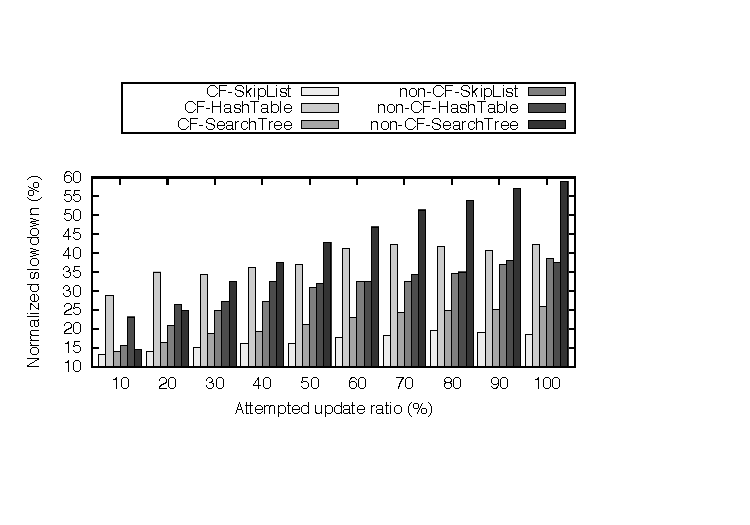
\includegraphics[scale=0.9,clip=true,viewport=10 50 280 230]{CF-general/experiments/pdf/updates}
\vspace{-1em}
\caption{\footnotesize{Tolerance to contention of Contention-Friendly (CF) and non-CF data structures (performance slowdown with respect to 0\% updates)\label{fig:updates}}}
\end{floatingfigure}
%
Interestingly, the slowdown of the CF hash table is higher than the one of the non-CF hash table at low 
levels of contention but becomes similar at high contention levels. 
As shown later, our CF hash table is actually very efficient on read-only workload whereas the ConcurrentHashMap relies on lock-stripes whose segments have to be loaded even on read-only workloads. 
This explains why CF performance drops as soon as contention appears, however, the CF hash table tolerates the contention increase as the slowdown remains almost constant, as opposed to the non-CF hash table.
We played with the number of segments and we observed better scalability with more segments but lower read-only overhead with a single one. We chose 64 segments which makes threads fetch multiple segments from memory before finding them in their cache. Another advantage of using  the CF hash table is not having to worry about such segments.

Figure~\ref{fig:perf} compares the performance of state-of-the-art data structures against performance of our CF data structures with $2^{14}$ (left) and $2^{16}$ elements (right) and on a read-only workload (top) and workloads comprising up to 30\% updates (bottom). While all data structures scale well with the number of threads, the state-of-the-art data structures are slower than their contention-friendly counterparts in all the various settings. In particular, the CF hash table, skip list, search tree are respectively up to $1.2\times$, $1.3\times$, $2.2\times$ faster than their non-CF counterparts.

Finally Appendix~\ref{sec:tm} shows that our adaptation of these data structures to three transactional memory algorithms allows a performance benefit of $1.5\times$ on average.

\begin{figure}
\begin{center}
\subfigure[$2^{14}$ elements\label{fig:214}]{\includegraphics[scale=0.45,clip=true,viewport=55 60 555 800]{CF-general/experiments/pdf/raw-perf-16384-60}}\hspace{0.5em}
%\caption{Performance of the Contention-Friendly (CF) and non-CF data structures with $2^{14}$ elements\label{fig:perf}}

\end{center}
\end{figure}
\begin{figure}
\begin{center}

\subfigure[$2^{16}$ elements\label{fig:216}]{\includegraphics[scale=0.45,clip=true,viewport=97 60 555 800]{CF-general/experiments/pdf/raw-perf-65536-60}}
%\caption{Performance of the Contention-Friendly (CF) and non-CF data structures with $2^{16}$ elements\label{fig:perf}}
\caption{Performance of the Contention-Friendly (CF) and non-CF data structures\label{fig:perf}}
\end{center}
\end{figure}



%\begin{figure}
%\begin{center}
%\includegraphics[scale=0.38]{experiments/pdf/raw-perf-16384-60}
%\caption{Performance of the Contention-Friendly (CF) and non-CF data structures with $2^{14}$ elements\label{fig:perf}}
%\end{center}
%\end{figure}
%
%\begin{figure}
%\begin{center}
%\includegraphics[scale=0.38]{experiments/pdf/raw-perf-65536-60}
%\caption{Performance of the Contention-Friendly (CF) and non-CF data structures with $2^{16}$ elements\label{fig:perf}}
%\end{center}
%\end{figure}


\section{Conclusion}\label{sec:conclusion}

Multicore programming brings new challenges, like contention, that programmers have to anticipate
when developing novel applications.
Programmers must now give up concentrating on the big-oh complexity and should
rather think in terms of contention overhead.
We explored the methodology of designing contention-friendly data structures, keeping in mind that contention will be a predominant cause of performance loss in tomorrow's architectures.
This simple methodology led to a novel Java package of concurrent data structures more efficient than the best implementations we could find. We plan to extend it with additional contention-friendly data structures.
%\vincent{Although transactions let the programmer take a pessimistic/sequential program as it is and make it concurrent, 
%the code requires to be significantly changed to be efficient.}

%\section*{Source Code}
%\sloppy{The Java code of the speculation-friendly library at \href{http://lpd.epfl.ch/gramoli/php/synchrobench.php}{http://lpd.epfl.ch/gramoli/php/synchrobench.php}.}
%
%\section*{Acknowledgements}
%The research leading to these results has received funding from the European Union Seventh Framework Programme (FP7/2007-2013) under grant agreement number 238639, ITN project TransForm, and grant agreement number 248465, the S(o)OS project.

% \newpage
% 
% \bibliographystyle{abbrv}
% \bibliography{bib}
% 
% \newpage
% 
% \begin{appendix}
% 
% % \section{Transactional Memory running CF skip list and CF binary search trees}\label{sec:tm}
% % \begin{figure*}
% % \begin{center}
% % 
\includegraphics[scale=0.5]{./fig/legend-stms}\\
% % \subfigure[CF-SkipList vs. Pugh Skip List]{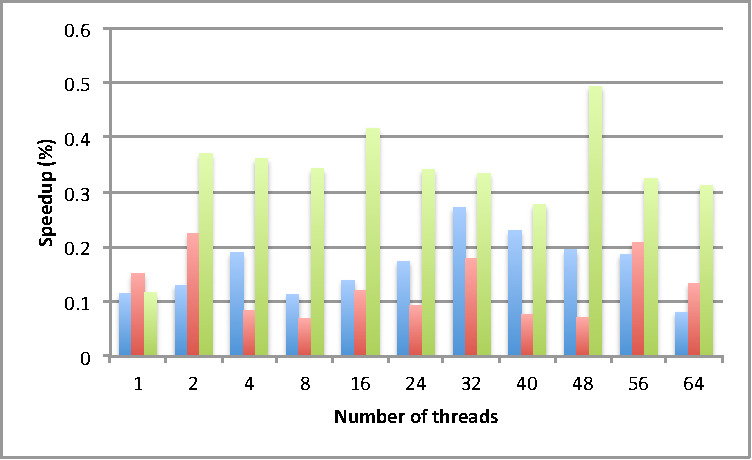
\includegraphics[scale=0.6]{./fig/skiplist-speedup}}
% % \subfigure[CF-Tree vs. RB-Tree]{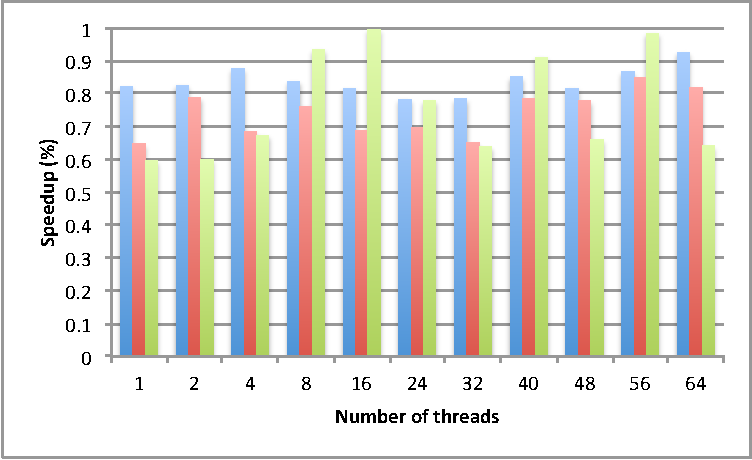
\includegraphics[scale=0.6]{./fig/tree-speedup}}
% % \caption{STM Speedup when using CF data structures instead of their existing counterparts on the Niagara 2 machine\label{fig:niagara2}}
% % \end{center}
% % \end{figure*}
% % 
% % \input alg/general3-1.tex
% 
% \input{appendix.tex}
% 
% \end{appendix}

%\section{Curves}
%
%\begin{figure*}
%\begin{center}
%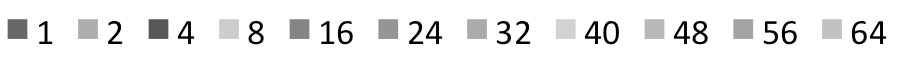
\includegraphics[scale=0.3]{./fig/legend-threadnum}
%\subfigure[$2^{12}$ elements, 0\% update]{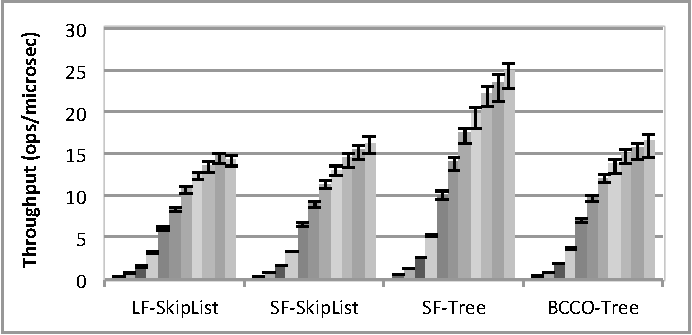
\includegraphics[scale=0.7]{./fig/nostms-logds-i4096-w0-bw.pdf}}
%\subfigure[$2^{12}$ elements, 10\% update]{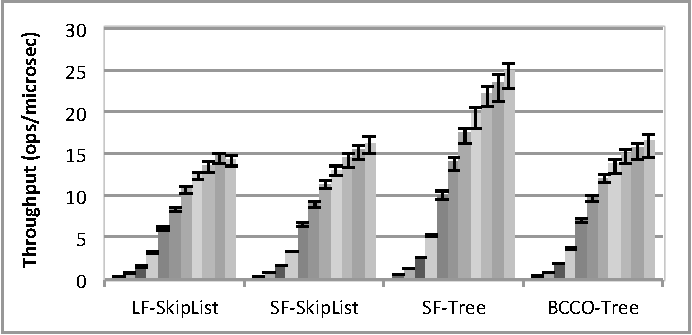
\includegraphics[scale=0.7]{./fig/nostms-logds-i4096-w0-bw.pdf}}
%\subfigure[$2^{12}$ elements, 20\% update]{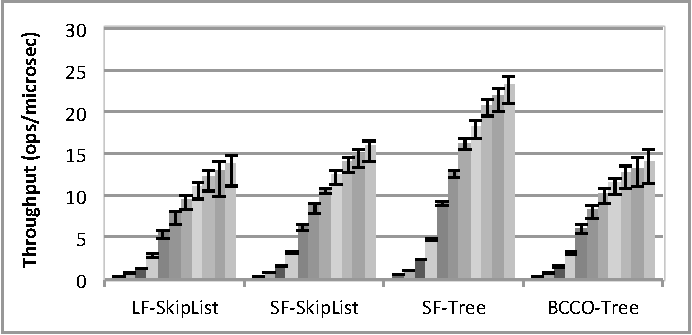
\includegraphics[scale=0.7]{./fig/nostms-logds-i4096-w10-bw.pdf}}
%\caption{Data structure (with logarithmic complexity) from the Niagara 2 machine\label{fig:niagara2}}
%\end{center}
%\end{figure*}

%\begin{figure*}
%\begin{center}
%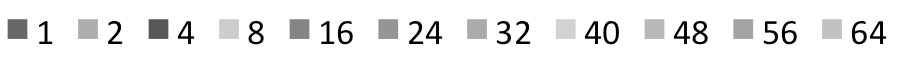
\includegraphics[scale=0.3]{./fig/legend-threadnum}
%\subfigure[$2^{14}$ elements, 0\% update]{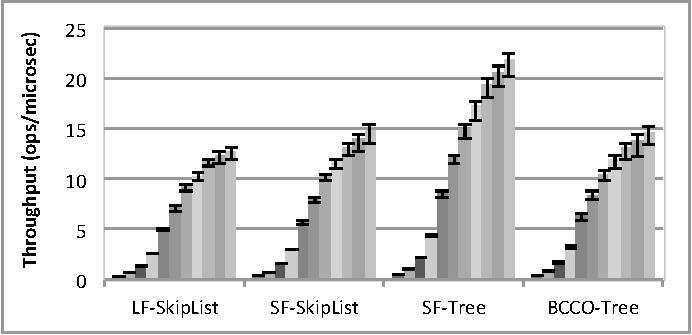
\includegraphics[scale=0.7]{./fig/nostms-logds-i16384-w0-bw.pdf}}
%\subfigure[$2^{16}$ elements, 0\% update]{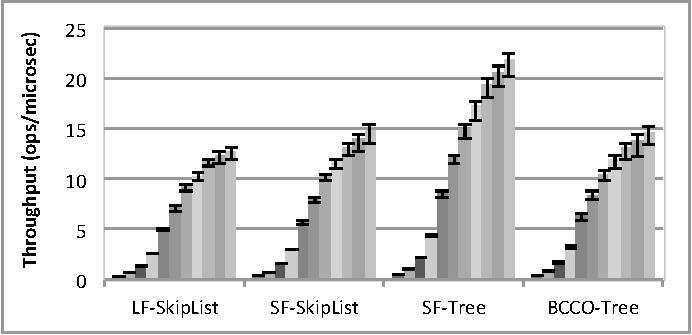
\includegraphics[scale=0.7]{./fig/nostms-logds-i16384-w0-bw.pdf}}
%\subfigure[$2^{14}$ elements, 10\% update]{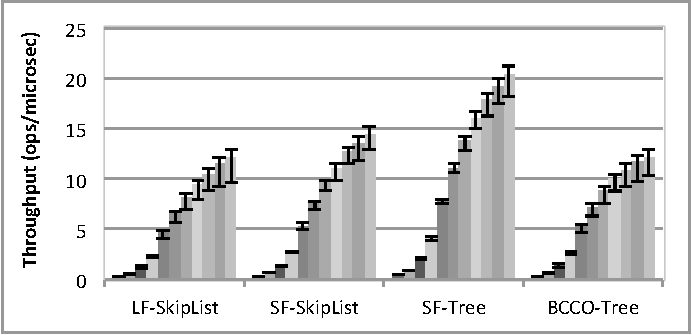
\includegraphics[scale=0.7]{./fig/nostms-logds-i16384-w10-bw.pdf}}
%\subfigure[$2^{16}$ elements, 10\% update]{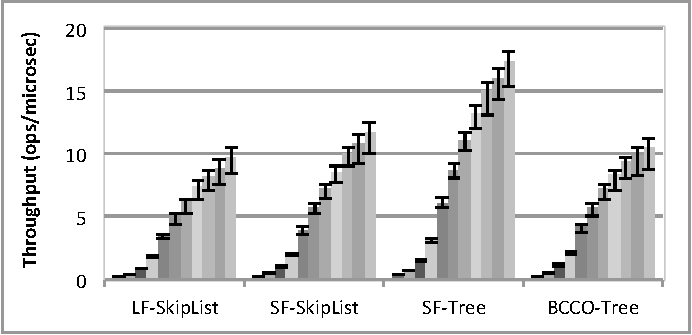
\includegraphics[scale=0.7]{./fig/nostms-logds-i65536-w10-bw.pdf}}
%\subfigure[$2^{14}$ elements, 20\% update]{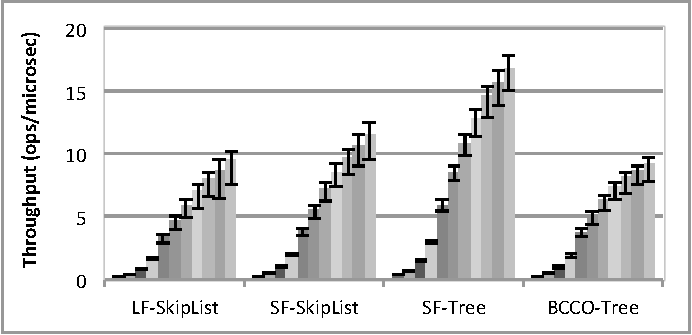
\includegraphics[scale=0.7]{./fig/nostms-logds-i65536-w20-bw.pdf}}
%\subfigure[$2^{16}$ elements, 20\% update]{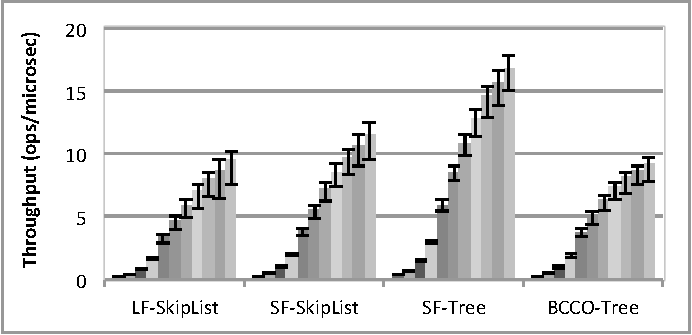
\includegraphics[scale=0.7]{./fig/nostms-logds-i65536-w20-bw.pdf}}
%\caption{Data structure (with logarithmic complexity) from the Niagara 2 machine\label{fig:niagara2}}
%\end{center}
%\end{figure*}


% Figure~\label{fig:niagara2} depicts the throughput performance obtained on the logarithmic data structures.
% 
% 
% \begin{figure*}
% \begin{center}
% 
\includegraphics[scale=0.4]{./fig/legend-skiplist}\\
% \subfigure[$2^{12}$ elements, 0\% update]{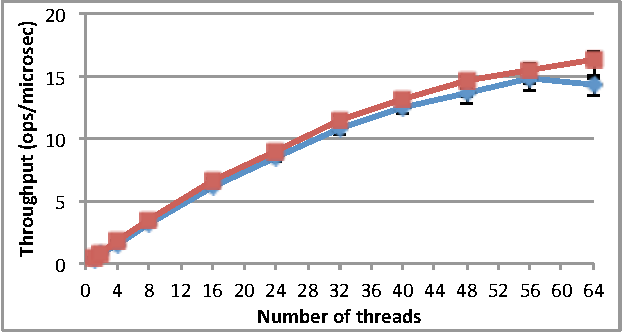
\includegraphics[scale=0.7]{./fig/nostms-sl-i4096-w0-bw.pdf}}\\
% \subfigure[$2^{12}$ elements, 10\% update]{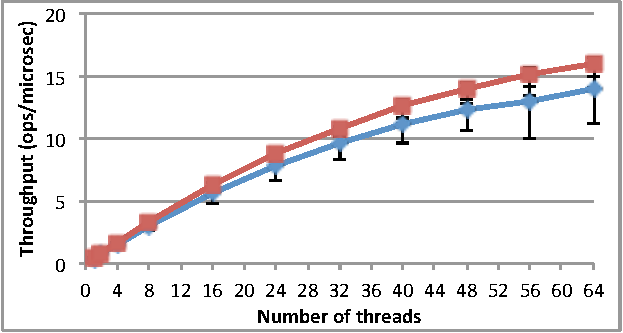
\includegraphics[scale=0.7]{./fig/nostms-sl-i4096-w10-bw.pdf}}\\
% \subfigure[$2^{12}$ elements, 20\% update]{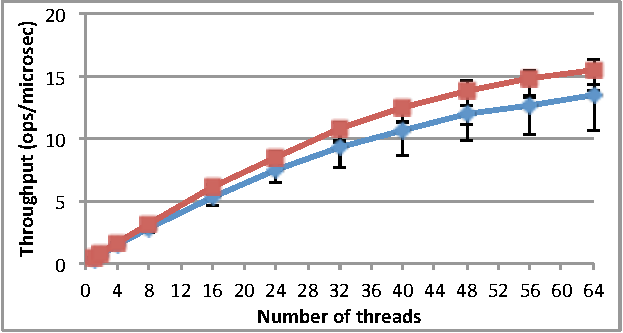
\includegraphics[scale=0.7]{./fig/nostms-sl-i4096-w20-bw.pdf}}
% \caption{Skip list results from the Niagara 2 machine\label{fig:niagara2}}
% \end{center}
% \end{figure*}
% 
% \begin{figure*}
% \begin{center}
% 
\includegraphics[scale=0.4]{./fig/legend-skiplist}\\
% \subfigure[$2^{14}$ elements, 0\% update]{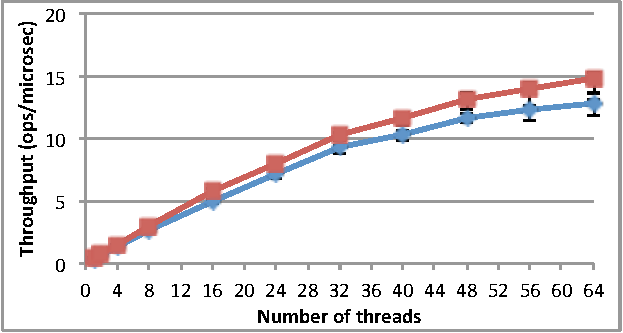
\includegraphics[scale=0.7]{./fig/nostms-sl-i16384-w0-bw.pdf}}
% \subfigure[$2^{16}$ elements, 0\% update]{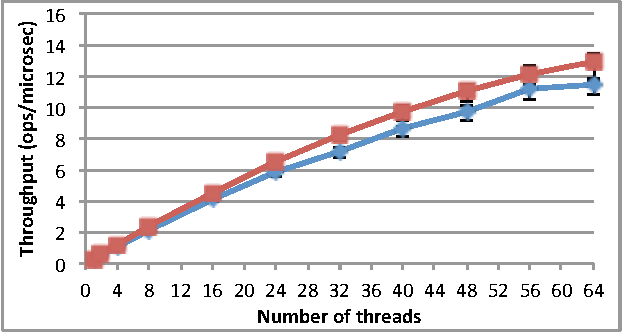
\includegraphics[scale=0.7]{./fig/nostms-sl-i65536-w0-bw.pdf}}
% \subfigure[$2^{14}$ elements, 10\% update]{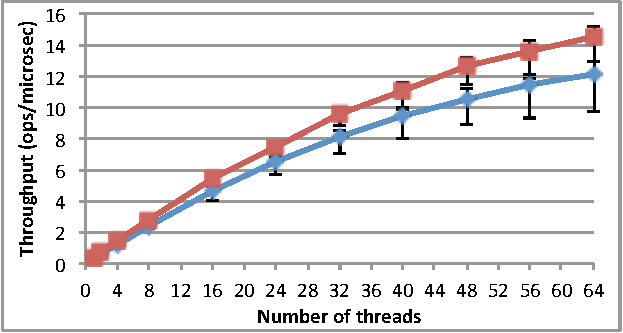
\includegraphics[scale=0.7]{./fig/nostms-sl-i16384-w10-bw.pdf}}
% \subfigure[$2^{16}$ elements, 10\% update]{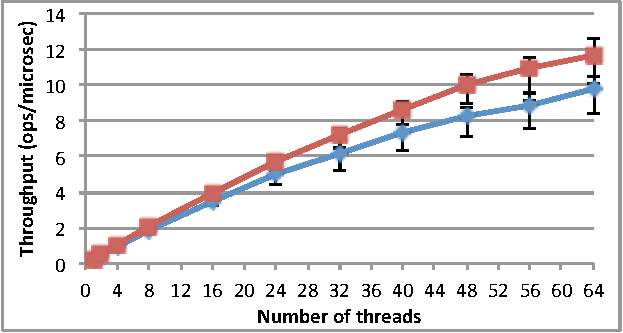
\includegraphics[scale=0.7]{./fig/nostms-sl-i65536-w10-bw.pdf}}
% \subfigure[$2^{14}$ elements, 20\% update]{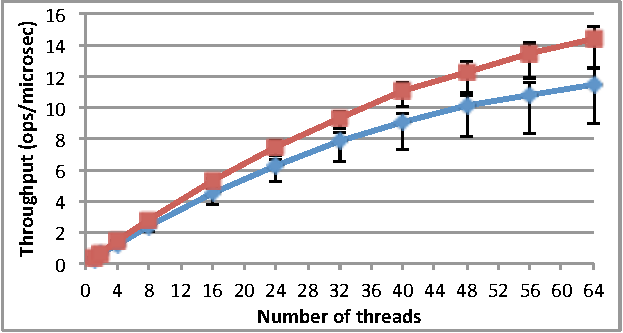
\includegraphics[scale=0.7]{./fig/nostms-sl-i16384-w20-bw.pdf}}
% \subfigure[$2^{16}$ elements, 20\% update]{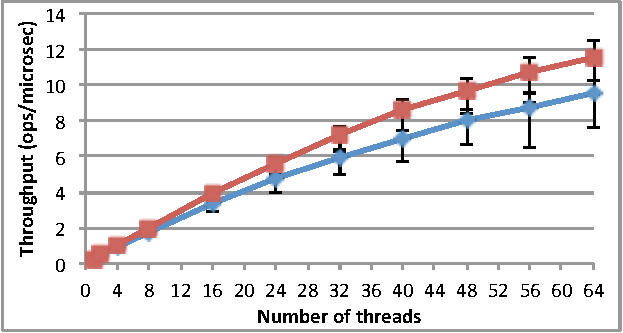
\includegraphics[scale=0.7]{./fig/nostms-sl-i65536-w20-bw.pdf}}
% \caption{Skip list results from the Niagara 2 machine\label{fig:niagara2}}
% \end{center}
% \end{figure*}
% 
% 
% \begin{figure*}
% \begin{center}
% 
\includegraphics[scale=0.4]{./fig/legend-hashtable-2}\\
% \subfigure[$2^{12}$ elements, 0\% update]{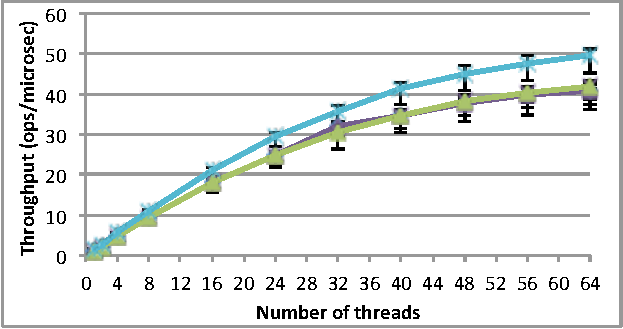
\includegraphics[scale=0.7]{./fig/nostms-ht2-i4096-w0-bw.pdf}}\\
% \subfigure[$2^{12}$ elements, 10\% update]{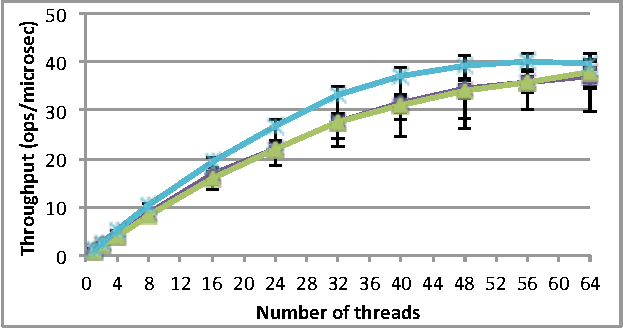
\includegraphics[scale=0.7]{./fig/nostms-ht2-i4096-w10-bw.pdf}}\\
% \subfigure[$2^{12}$ elements, 20\% update]{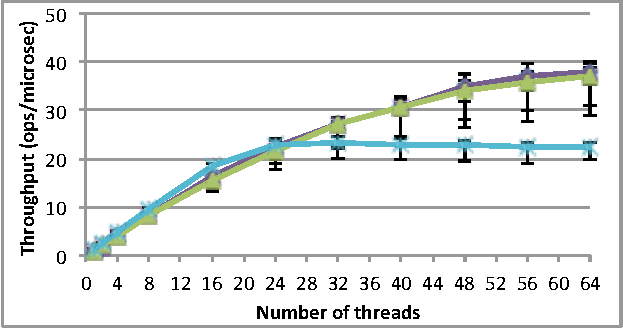
\includegraphics[scale=0.7]{./fig/nostms-ht2-i4096-w20-bw.pdf}}
% \caption{Hash table results from the Niagara 2 machine\label{fig:niagara2}}
% \end{center}
% \end{figure*}
% 
% 
% \begin{figure*}
% \begin{center}
% 
\includegraphics[scale=0.4]{./fig/legend-hashtable-2}\\
% \subfigure[$2^{14}$ elements, 0\% update]{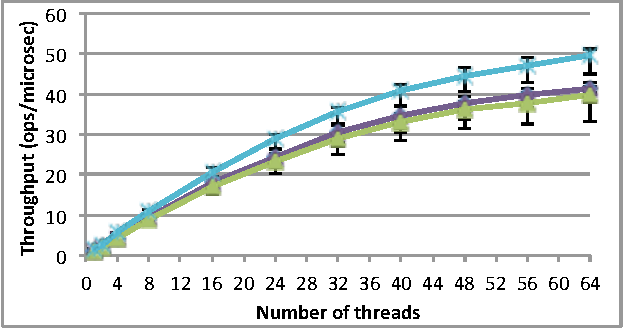
\includegraphics[scale=0.7]{./fig/nostms-ht2-i16384-w0-bw.pdf}}
% \subfigure[$2^{16}$ elements, 0\% update]{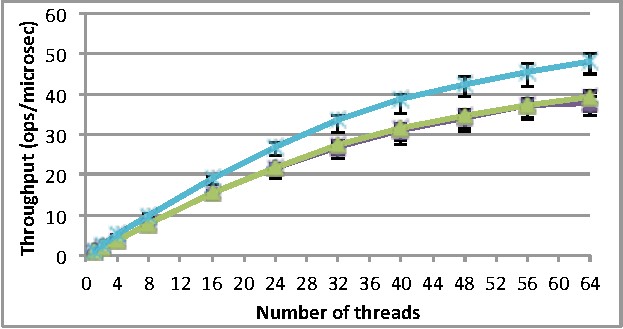
\includegraphics[scale=0.7]{./fig/nostms-ht2-i65536-w0-bw.pdf}}
% \subfigure[$2^{14}$ elements, 10\% update]{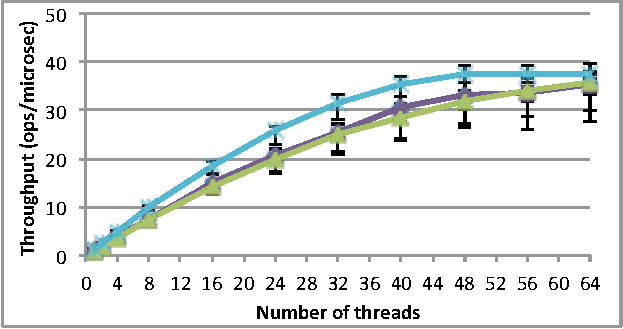
\includegraphics[scale=0.7]{./fig/nostms-ht2-i16384-w10-bw.pdf}}
% \subfigure[$2^{16}$ elements, 10\% update]{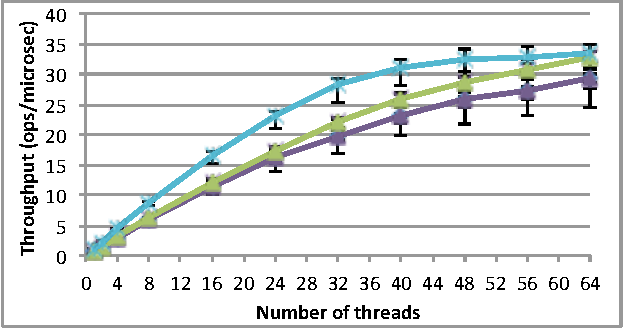
\includegraphics[scale=0.7]{./fig/nostms-ht2-i65536-w10-bw.pdf}}
% \subfigure[$2^{14}$ elements, 20\% update]{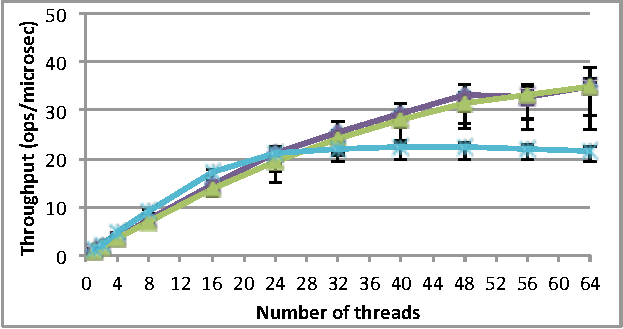
\includegraphics[scale=0.7]{./fig/nostms-ht2-i16384-w20-bw.pdf}}
% \subfigure[$2^{16}$ elements, 20\% update]{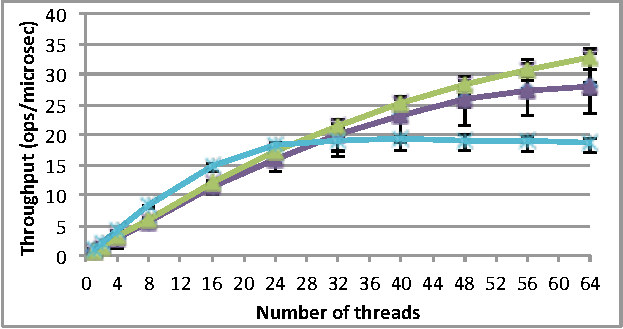
\includegraphics[scale=0.7]{./fig/nostms-ht2-i65536-w20-bw.pdf}}
% \caption{Hash table results from the Niagara 2 machine\label{fig:niagara2}}
% \end{center}
% \end{figure*}
% 
% 
% \begin{figure*}
% \begin{center}
% 
\includegraphics[scale=0.4]{./fig/legend-tree}\\
% \subfigure[$2^{12}$ elements, 0\% update]{\includegraphics[scale=0.7]{./fig/nostms-tree-i4096-w0-bw.pdf}}\\
% \subfigure[$2^{12}$ elements, 0\% update]{\includegraphics[scale=0.7]{./fig/nostms-tree-i4096-w0-bw.pdf}}\\
% \subfigure[$2^{12}$ elements, 10\% update]{\includegraphics[scale=0.7]{./fig/nostms-tree-i4096-w10-bw.pdf}}
% \caption{Binary tree results from the Niagara 2 machine\label{fig:niagara2}}
% \end{center}
% \end{figure*}
% 
% 
% \begin{figure*}
% \begin{center}
% \includegraphics[scale=0.4]{./fig/legend-tree}\\
% \subfigure[$2^{14}$ elements, 0\% update]{\includegraphics[scale=0.7]{./fig/nostms-tree-i16384-w0-bw.pdf}}
% \subfigure[$2^{16}$ elements, 0\% update]{\includegraphics[scale=0.7]{./fig/nostms-tree-i65536-w0-bw.pdf}}
% \subfigure[$2^{14}$ elements, 10\% update]{\includegraphics[scale=0.7]{./fig/nostms-tree-i16384-w10-bw.pdf}}
% \subfigure[$2^{16}$ elements, 10\% update]{\includegraphics[scale=0.7]{./fig/nostms-tree-i65536-w10-bw.pdf}}
% \subfigure[$2^{14}$ elements, 20\% update]{\includegraphics[scale=0.7]{./fig/nostms-tree-i16384-w20-bw.pdf}}
% \subfigure[$2^{16}$ elements, 20\% update]{\includegraphics[scale=0.7]{./fig/nostms-tree-i65536-w20-bw.pdf}}
% \caption{Binary tree results from the Niagara 2 machine\label{fig:niagara2}}
% \end{center}
% \end{figure*}
% 
% 
% \begin{figure*}
% \begin{center}
% \includegraphics[scale=0.6]{./fig/legend-restructuring}\\
% \includegraphics[scale=0.7]{./fig/restructuring.pdf}
% \caption{Amount of restructuring observed on the Niagara 2 machine\label{fig:niagara2}}
% \end{center}
% \end{figure*}




% \end{document}



\section{Transactional Contention-Friendly Algorithms}\label{sec:tm} 


The concept of splitting the abstract operation and the structural modification to create contention friendly data structures
does not only apply to lock based or lock-free implementations.
It can also be applied to data structures implementations using transactional memory.
Our previous work has studied this problem when specifically looking at trees \cite{CGR12}.

%Figure \ref{fig:niagara2} shows the speedup of the contention friendly algorithms in transactional memory as compared
%to a red black tree and the Pugh Skip List which were converted from their sequential counterparts by placing their operations within transactions.
%In order to perform these tests we used the bytecode instrumentation 
%framework Deuce~\cite{KSF10}. Although this framework adds a significant overhead to the execution time, it greatly 
%simplifies the usage of various transactional memory algorithm. We have run the tests using the TM systems 
%TL2~\cite{DSS06}, LSA~\cite{RFF06}, and ${\mathcal E}$-STM~\cite{FGG09} illustrating the 
%portability of contention friendly data structures to TM systems satisfying the standard TM interface~\cite{abi}.
We now present the experimental results with three existing transactional memory implementations:
${\mathcal E}$-STM~\cite{FGG09}, LSA~\cite{RFF06} and TL2~\cite{DSS06} using the Deuce Java bytecode instrumentation framework~\cite{KSF10}.
The experimental settings are the same as for other experiments, except that we evaluate the red-black tree (non-CF tree) and the Pugh skip list (non-CF skip list) to compare our CF tree and CF skip list against on $2^{12}$ elements with 5\% effective updates.
Figure~\ref{sfig:tm-sl} and Figure~\ref{sfig:tm-rt}  depict the speedup of using the CF skip list over using the non-CF skip list (resp. CF tree over using the non-CF tree)
for each of the considered transactional memory implementations.
Using transaction-based CF data structures as opposed to default ones clearly speeds up the performance of all transactional memories. The benefit of turning to CF is more important when using trees, which confirms our previous results obtained with our lock-based implementations. In particular, the average speedup for all transactional memories and data structures is of 50\%.
Interestingly, the speedup of using transaction-based CF does not scale much with the number of threads, probably because the overhead induced by transactional memory and Deuce is too heavy for the contention rise to be visible.

When using transactional memory the benefit of these contention friendly algorithms is apparent just
by the fact that abstract operation transactions will have smaller read and write sets causing less contention
on the data structure and making the operations less likely to abort.
Also structural modifications are each broken into a single transaction causing less contention then they would
be if they were include in a single large transaction.

The abstract operations for the tree are very simple, traversals are done in the same way they would be in a
sequential algorithm except transactional reads are used.
Each physical removal and rotation is performed as a single transaction by the structural adaptation.

In the lock based version of the skip list locks are only used when traversing the bottom level of
the structure.
Each of the index levels are accessed and modified using only regular read/write operations.
This can be applied to the transaction version of the skip list as well.
Abstract operation traversals as well as structural modifications to the index level are done outside of transactions.
Once an abstract operation traversal has reached the bottom list level a transaction is started, if it arrived on
a physically removed node then the operation travels backwards in the list until is reaches a node still in the structure
at which point the traversal continues as it would in a sequential list algorithm.
Physical removals are done as single transactions by the structural adaptation.

The transactional hash table is very similar to the to the lock-free contention friendly version.
Each abstract operation is contained in a single transaction where the $\lit{compare\&swap}$
operations from the lock-free version are replaced by reads and writes.
During the rehash operation each bucket rehash is done as a single transaction.



\begin{figure*}
\begin{center}
%\includegraphics[scale=0.5]{./fig/legend-stms}\\
\subfigure[CF-SkipList vs. Pugh Skip List\label{sfig:tm-sl}]{\includegraphics[scale=0.85,clip=true,viewport=10 50 280 200]{CF-general/experiments/pdf/tm-skiplist}}
\subfigure[CF-Tree vs. RB-Tree\label{sfig:tm-rt}]{\includegraphics[scale=0.85,clip=true,viewport=10 0 280 200]{CF-general/experiments/pdf/tm-tree}}
\caption{STM Speedup when using CF data structures instead of their existing counterparts on the Niagara 2 machine\label{fig:niagara2}}
\end{center}
\end{figure*}


\section{Pseudo-code and Description}\label{app:pseudocode}

% \remove {
% 
% \subsection{Linked List}
% 
% \input alg/list_op.tex
% 
% \subsubsection{Non-maintenance Operations}
% The code for these operations is found in figure \ref{alg:list_op}.
% 
% The list nodes are standard doubly linked linked list nodes.
% To access the list there is a pointer $\ms{first}$ to the first node in the list.
% To simplify the algorithm the first node in the list is never removed and has key $\neg \inf$.
% 
% The traversal is very similar to the standard list traversal algorithm with one exception.
% When a traversal notices that is has reached a node that has been physically removed from the 
% structure (has $\ms{removed}$ flag set to $\lit{true}$)
% it travels backwards in the list (using the $\ms{prev}$ pointer) until it reaches a node that is 
% not removed.
% This is done to ensure that the traversal never passes the node it is searching for.
% 
% When adding an item to the list, the node that will be the node just before the new node is locked and the
% new node is inserted.
% 
% \input alg/list_maint.tex
% 
% \subsubsection{Maintenance Operations}
% The code for these operations is found in figure \ref{alg:list_maint}.
% Only maintenance needed for the list is performing physical removal.
% 
% To preform the removal, first the node to be removed and the node before it in the list is locked, then
% the $\ms{deleted}$ flag is check and the node is removed by changing the previous node's
% next pointer point to the next node and the previous pointer of this node is updated.
% Finally the node's removed flag is set to $\lit{true}$ and the nodes are unlocked.
% 
% }

All three data structures share the general structural adaptation code shown in Algorithm~\ref{alg:state-and-maintenance}.

In the normal case the structural adaptation thread works by performing the
$\ms{background-struct-adaptation}$ operation constantly traversing the data structure
by calling the $\ms{restructuring}$ procedure.
Each iteration of this procedure traverses the entire data structure where at each node it might perform some sort of restructuring or a removal.
For some data structures after a complete traversal of the structure is done, some restructuring of the entire structure might be needed,
this includes the rehash operation of a hash table or the changing of levels of nodes in the skip list.

For backwards compatibility the structural adaptation can also be distributed among the program threads by calling the 
$\ms{distributed-struct-adaptation}$ operation.
In this case each $\ms{insert/delete}$ operation will toss a coin, if the value of this coin is greater then some threshold value
the thread will then acquire a global structural adaptation lock, and call the $\ms{restructuring}$ procedure before finally
releasing the lock, and continuing with its abstract operation.


\subsection{Tree and Skip List}

\paragraph{Skip List}
As with existing skip list algorithms the structure is made up of many levels of linked lists.

The bottom level of is made up of a doubly linked list of nodes.
Each node has a $\ms{prev}$ and $\ms{next}$ pointer, as well as pointer to its key $\ms{k}$,
an integer $\ms{level}$ indicating the number of levels of linked lists this node has,
the $\ms{rem}$ and $\ms{del}$ flags, and a lock.

The upper levels are made up of singly linked lists of IndexItems.
Each of these items has a $\ms{next}$ pointer, pointing to the next item in the linked list.
A $\ms{down}$ pointer, pointing to the linked list of IndexItems one level below (the bottom level
of IndexItems have $\bot$ for their $\ms{down}$ pointers).
And a $\ms{node}$ pointer that points to the corresponding node in the Speculation Friendly Skip List.

A per structure array of pointers called $\ms{first}$ is also kept that points to the first element of each level
of the skip list.
The pointer $\ms{top}$ points to the first element of the highest index of the list, all traversals
start from this pointer.

\paragraph{Tree}
The tree is made up of nodes with each node having left and right child
pointers $\ms{l}$ and $\ms{r}$, as well as a pointer to its key $\ms{k}$,
integers indicating the estimated local height
of this node and its children $\ms{left-h}$, $\ms{right-h}$, and $\ms{local-h}$,
the $\ms{rem}$ and $\ms{del}$ flags, and a lock.

In addition there is a single pointer $\ms{root}$ that points to the root node of
the tree.

\subsubsection{Skip List Structural Adaptation}

\input CF-general/alg/skipList_maint.tex

The code for the skip list structural adaptation operations is found in Algorithm~\ref{alg:skipList_maint}.

The $\ms{restructure-node}$ procedure takes care of removing marked deleted nodes.
For each node it checks if it has both a level of $0$ and $\ms{del}$ set to $\lit{true}$
then tries to remove the node by calling the $\ms{remove-node}$ procedure.
This procedure locks both the node to be removed and the node previous to it in the list in order
to not conflict with concurrent $\ms{insert}$ and $\ms{delete}$ operations.
The node is then simply removed by changing the previous node's pointer to skip the node.
Finally the $\ms{rem}$ flag is set to true and the locks are released.

The $\ms{restructure-structure}$ procedure raises and lowers the levels of the nodes in order
to keep the logarithmic traversal cost of the abstract operations.
This is done by calling the $\ms{raise-node-level}$ procedure on the bottom level of the
skip list and the $\ms{raise-index-level}$ on higher levels.
The code for the procedures is practically the same, just $\ms{raise-node-level}$ is performed
on nodes while $\ms{raise-index-level}$ is performed on index levels as such only the 
$\ms{raise-index-level}$ pseudo code is displayed here.
The procedures work by simply traversing the entire level $\ms{i}$ that they are called on
if they encounter $3$ or more nodes all with height $\ms{i}$ then the middle of these
nodes is raised to height $\ms{i+1}$.
This is performed on each index level starting from the bottom until there are less than $2$
nodes on a level.

Due to nodes being removed from the skip list it might be necessary to decrease
the number of index levels in the structure.
If the $log$ of the number of nodes in the structure is less then the height of
the structure then the bottom index level is removed.
This is done by the $\ms{lower-index-level}$ procedure which simply traverses
the second from bottom index level and sets each index item's $\ms{down}$ pointer to $\bot$.
Finally the index of the $\ms{first}$ array must be updated to take account
the removal of the bottom index level.

\input CF-general/alg/tree_maint.tex

\subsubsection{Tree Structural Adaptation} \label{sec:treemaint}
The code for these operations is found in Algorithm~\ref{alg:tree_maint}.

The $\ms{restructure-node}$ procedure takes care of removing marked deleted nodes as well as
performing rotations and propagating balance information upwards in the tree.

Like in the skip list only certain nodes are removed.
These are the nodes that have $1$ or $0$ children and are a majority of the nodes in the tree.
This avoids expensive removal operations that require finding
and moving a successor node.

In order to do a removal first the parent and the node to be removed are locked(in order to
prevent conflicts with concurrent $\ms{insert}$ and $\ms{delete}$ operations) and the
$\ms{del}$ flag of the node is checked.
The node to be removed has its $\ms{left}$ and $\ms{right}$ child pointers changed so that they point to the parent.
This is done to ensure a concurrent operation preempted on this node can still proceed.
Next the appropriate parent's child pointer is changed to point to the non-null child of the node to be removed
(if any).
Finally the $\ms{rem}$ flag is set to $\ms{true}$.

% 
% \begin{figure*}
% 	%\vspace{-1em}
% 	\begin{center}
% 	\subfigure[Initial tree\label{sfig:tree1}]{\includegraphics[scale=0.4]{fig/tree1b}}\hspace{4em}
% 	\subfigure[Result of usual right rotation\label{sfig:tree2}]{\includegraphics[scale=0.4]{fig/tree2b}}\hspace{4em}
% 	\subfigure[Result of new right rotation\label{sfig:tree3}]{\includegraphics[scale=0.4]{fig/tree3b}}
% 	\caption{The classical rotation modifies node $j$ in the tree and forces a concurrent traversal at this node to backtrack. 
% 	The new rotation left $j$ unmodified, adds $j'$ and postpones the 
% 	physical deletion of $j$.\label{fig:rotation}}
% 	\end{center}
% 	%\vspace{-1em}
% \end{figure*}


The structural adaptation is also responsible for keeping the tree well balanced.
This is done by doing local rotations.
Deciding to do a rotation is based on a local estimated height values.
The height values are propagated from the leaves to the root by the $\ms{propagate}$ procedure.
This procedure is executed per node and simply reads the $\ms{l-height}$ values of its left
and right children, before updating its local values and setting its local $\ms{l-height}$ value
to $1$ greater then the maximum height of its children.
If the absolute value of a nodes left and right heights is at least two
then an appropriate rotation is performed.
Double rotations are performed as two separate single rotations.

In a traditional rotation operation one node is always rotated downwards.
If a concurrent traversal operation is preempted on this node then either it might have to abort
or rollback in order to ensure it performs a valid traversal or nodes must be locked/marked during traversal.

In order to avoid using locks and aborts/rollbacks, rotations are preformed differently then traditional rotations.
A diagram of the new rotation operation is shown in figure \ref{sfig:tree3}.
Before performing the rotation the parent node and the node $\ms{n}$ that will be rotated are locked in order to
prevent conflicts with concurrent $\ms{insert}$ and $\ms{delete}$ operations.
Instead of actually modifying $\ms{n}$, a new node $\ms{new}$ is created that takes $\ms{n}$'s place in the structure,
this node is set have the same values and pointers as $\ms{n}$ would if a rotation was performed as in
existing tree data structures.
After the rotation, the node $\ms{n}$ has its $\ms{rem}$ flag set (to $\lit{true}$ in the case of a right rotation
and $\lit{by-left-rot}$ in the case of a left rotation) and the locks are released.

The reason for not modifying $\ms{n}$ is so that concurrent traversals are not set off track.
If the node $\ms{n}$ is removed by a right (resp. left) rotation then its left (resp. right) child has a path to
all the nodes as it did before the rotation so a traversal preempted on this node can still traverse the tree safely.

\input CF-general/alg/general3-1.tex
\input CF-general/alg/general3-2.tex
\subsection{Abstract Operations}

The tree and skip list share code for the $\ms{contains}$, $\ms{insert}$, $\ms{delete}$ operations
displayed in Algorithm~\ref{alg:general_op-2}.
These operations might call one of more of the $get\_first$, $get\_next$, $validate$, $add$
procedures which each have specific code for the given data structure,
show in Algorithm~\ref{alg:tree_op} for the tree and Algorithm~\ref{alg:skipList_op}
for the skip list.
None of these additional procedures use locks or other synchronization methods.

\input CF-general/alg/skipList_op.tex
\input CF-general/alg/tree_op.tex

Each of the three abstract operations start by calling the $\ms{get\_first}$ procedure.
This operation returns the root of the tree or the first node of the top index level of the skip list.
The operations then traverse the structure using the $\ms{get\_next}$ procedure.
This procedure either returns the next node in the traversal or $\bot$ if the traversal is done.

The $\ms{get\_next}$ procedure traverses the tree by returning the right child if the node's key is lager then $k$
otherwise the left child is returned.
If the nodes key is equal to $\ms{k}$ and the node is not physically removed then $\bot$ is returned.
Since locks are not used during traversal the algorithm has to be aware of concurrent rotations.
This means returning the right child in case of being preempted on a node that was removed during a left rotation.
If the node was removed during a right rotation then the traversal can continue as normal unless it arrives at a
child pointer with value $\bot$, in this case it just returns the other child (which is guaranteed to not be $\bot$).

For the skip list the $\ms{get\_next}$ procedure traverses the structure just as it would in a sequential
algorithm, with the simple exception that is travels backwards in the list using the $\ms{prev}$ pointer
in the case of arriving at a node that has been physically removed.
If the nodes key is equal to $\ms{k}$ and the node is not physically removed or if the traversal
is at the bottom level and the next node has key greater then $\ms{k}$ then $\bot$ is returned.

Once $\bot$ is returned $\ms{insert}$ and $\ms{delete}$ operations protect the last node in the traversal by locking it (locking is not necessary for the $\ms{contains}$ operations as
it does not make modifications).
Due to concurrent operations this node may not longer be the end of the traversal, therefore the $\ms{validate}$ procedure is performed on this node
ensuring that the traversal has stopped at the correct location.
The validation checks to make sure that the node has not been physically removed and that no new node has been inserted directly after this node.

If the validation succeeds then the traversal is finished.
Otherwise the lock protecting the node
is released and the traversal continues.

Finally some additional code is executed depending on the operation.

In the case of a $\ms{contains}$ operation, the key and/or the deleted flag of the node is checked and a boolean is returned.

In the case of the $\ms{insert}$ operation, first the key of the node is checked, if it is equal to the key being search for then
the deleted flag of the node is checked (and possibly modified) and a boolean is returned.
Otherwise if the key is not equal to the one being searched for then the $\ms{add}$ operation is performed.
The code for the $\ms{add}$ operation simply allocates a new node and attaches
it to the data structure by modifying a pointer.

In the case of the $\ms{delete}$ operation the key of the node is checked, if it is equal to the key being search for then
the deleted flag of the node is checked (and possibly modified) and a boolean is returned.
Otherwise $\lit{false}$ is returned.
It should be noted that when these structures are used as maps the deleted flag can be replaced with a pointer to the
value object (from the key/map pair).
When this pointer is set to $\bot$ the node is considered as deleted.



\subsection{Hash Table}

The hash table is made up of two pointers to tables:
$\ms{table}$ and $\ms{new\_table}$.
The second is used during resize operations.
Each process also keeps local variable $\ms{l\_pointer}$ that points to a table.

Each table contains an array, with each location in the array containing a list of nodes.
Each location in the array is initialized to point to $\bot$.
The array also has a single special node associated with it called the $\ms{dummy}$ node which is used
during resizing.

\input CF-general/alg/hashTable_op.tex

\subsubsection{Abstract Operations}
The code for these operations is found in Algorithm~\ref{alg:hashTable_op}.
Each abstract operation starts by calculating the hash value of the key and then calling
the $\ms{get-first}$ procedure.
This procedure returns the first node in the table located at the bucket given by the hash value
or $\bot$ in the case that this bucket is empty.
The $\ms{get-first}$ procedure might encounter a dummy node, this means that there is a rehash operation
going on that has rehashed this bucket, but not yet finished rehashing the entire table.
In this case the local table pointer is updated and the bucket is read again.

Once a value is received from the $\ms{get-first}$ procedure the $\ms{contains}$ simply traverses
the list looking for a node with key $\ms{k}$.

The $\ms{insert}$ operation also traverses
the list looking for a node with key $\ms{k}$, if none is found then a new node is allocated and is
added to the beginning of the list by performing a $\lit{compare\&swap}$ on the bucket.
If the $\lit{compare\&swap}$ fails then the operation restarts.

If the $\ms{delete}$ operation locates a node $\ms{n}$ with key $\ms{k}$ in the list
then it creates a copy of the list from the first node in the list up to node $\ms{n}$ but not including $\ms{n}$.
The bucket is then set to first node of this list by performing a $\lit{compare\&swap}$.
If the $\lit{compare\&swap}$ fails then the operation restarts.


\input CF-general/alg/hashTable_maint.tex

\subsubsection{Structural Adaptations}
The code for these operations is found in Algorithm~\ref{alg:hashTable_maint}.
Local node restructuring is not necessary for the hash table.

The structure restructuring consists of two procedures.
The first is the $\ms{size}$ operation that simply traverses the structure
counting the number of nodes.
If the number of nodes has surpassed some threshold then a resize is necessary
and the $\ms{grow}$ procedure is called.
This procedure starts be creating a new table larger then the previous one
by a power of $2$.
It then goes through the old table rehashing one bucket at a time.
At each bucket in the old table it performs the $\ms{grow-level}$ procedure.
This procedure makes a copy of each node in the bucket, rehashing them and placing them
in their appropriate buckets in the new hash table.
The operation then replaces the list in the old table with its dummy node by performing a
$\lit{compare\&swap}$.
If the compare and swap fails then the operation is restarted for this level.
Once all levels have been rehashed the $table$ pointer is modified so that it points
to the new table.

\section{Correctness}\label{sec:proof}






Here we present a sketch of the proof that each data structure algorithm satisfies linearizability.

\subsection{Skip List}

Each of the $\ms{contains}$, $\ms{insert}$, and $\ms{delete}$ operations call the $\ms{validate}$ procedure.
The $\ms{validate}$ procedure may be called multiple times, but it must return $\lit{true}$ exactly once.
This is used as the linearizability point for the proof sketch.
Assume $\ms{k}$ the key provided as input to the abstract operation.

The result of the $\ms{contains}$, $\ms{insert}$, and $\ms{delete}$ operations depends on the existence of
a node with key $\ms{k}$
in the set described by the data structure.
At any single point in time there is exactly one valid location in the list where a node with key $\ms{k}$ can exist
(Note that a full proof would require to show this, for example by induction).
This location is the $\ms{next}$ pointer of the node in the list with the largest key smaller then $\ms{k}$.
For the purpose of this proof sketch we will use a node (call this node $\ms{corr}$) that is either the node in the list
with key $\ms{k}$ or if no node with key $\ms{k}$ exists the node whose $\ms{next}$ pointer would point to the node with key $\ms{k}$.

Any operation that modifies a node must lock the node before it performs any modification.
Given that the $\ms{validate}$ operation is called while a node is locked it only needs to be shown
that the when $\ms{validate}$ returns $\lit{true}$ the node locked is $\ms{corr}$.

The nodes in the list are sorted by their keys and the $\ms{prev}$ pointer is not modified when a node is removed
so any removed node will always have a path to a non-removed node with a smaller or equal key.
This means that there will always be a path from a node with key smaller then or equal to $\ms{k}$ to $\ms{corr}$.
Now since the $\ms{get-next}$ procedure will never traverse past a node that has key larger then $\ms{k}$ the operation it will always have
a path to $\ms{corr}$.
If a node that has been removed is reached during traversal the $\ms{prev}$ pointer is followed, otherwise the $\ms{next}$ pointer
is followed during traversal so $\ms{corr}$ will be reached eventually.

Before the $\ms{validate}$ operation returns $\lit{true}$ it first ensures that the locked node has either key $\ms{k}$ or the node pointed
to by the locked node's $\ms{next}$ pointer has a key larger then $\ms{k}$.
Second it ensures that the node is not removed ($\ms{rem}=\lit{false}$).
Therefore when $\ms{validate}$ returns $\lit{true}$, the locked node must be $\ms{corr}$.

\subsection{Tree}
The tree is a bit more complicated because traversals have to deal with
rotations as well as removals.
Like in the skip list the abstract operations can call the $\ms{validate}$ procedure multiple times, but it must return $\lit{true}$ exactly once.
This is used as the linearizability point for the proof sketch.
Assume $\ms{k}$ is the key provided as input to the abstract operation.

At any point in time there is exactly one valid location in the tree where a node with key $\ms{k}$ can exist.
This location is the left or right child pointer of a certain node.
This pointer points to the node with key $\ms{k}$ or to $\bot$ if no node with key $\ms{k}$ exists.
For the purpose of this proof sketch we will use a node (call this node $\ms{corr}$) that is either the node with
this pointer (if no node with key $\ms{k}$ exists) or the node with key $\ms{k}$ (is a node with key $\ms{k}$ does exist).

Before the $\ms{validate}$ operation returns $\lit{true}$ it first ensures that the locked node either has key $\ms{k}$ or
(if the locked node does not have key $\ms{k}$) the
child pointer from the locked node where $\ms{k}$ would exist is $\bot$.
Second it ensures that the locked node is not removed ($\ms{removed}=\lit{false}$).

Now to complete the sketch it is enough to show that the traversal never passes $\ms{corr}$.
Without rotations or removals this is simple.
With removals and rotations the idea is to show that a traversal that is preempted on a node modified by a removal or rotation
operation has a path to a node at a higher level in the tree so that the traversal still has a path to $\ms{corr}$.
For removals this is clear due to the fact a removed node has both its child pointers point to its parent during removal.
Rotations require a bit more detail.
In a traditional left/right rotation one node is rotated downward in the tree while either its left or
right child is rotated upwards.
For rotations in the contention friendly algorithm the child pointers of the node that
would normally be rotated downwards (call this node $\ms{n}$) are not modified at all.
Instead $\ms{n}$ is removed from the tree (as the previous parent of $\ms{n}$ now points to one of $\ms{n}$'s children)
and a new node is created taking $\ms{n}$'s place.
This new node is set up exactly how $\ms{n}$ would be after a traditional rotation.
Now since one of $\ms{n}$'s children was rotated upwards any concurrent traversal preempted on $\ms{n}$ will
still have a path to all the nodes it did before the rotation.

\subsection{HashTable}
The linearization of the hash table relies on two things, first that the $next$ pointer of a node is never modified
after it is set during creation, and second any successful modification to a bucket happens by performing a
single $\ms{compare\&swap}$ on the bucket's pointer.

The linearization point of the $\ms{contains}$ operation is when the $\ms{get-first}$ procedure reads the first element of the
bucket that is later returned.
Since the next pointer of nodes is never changed then when the operation traverses the list it observes a valid state of the list.
The same is true for $\ms{insert}$ and $\ms{delete}$ operations that complete without performing a $\ms{compare\&swap}$.

If a $\ms{compare\&swap}$ is required, then the lineraization point is when the $\ms{compare\&swap}$ returns successfully.
Given that the $\ms{compare\&swap}$ operations are only performed at the first element of the bucket, if the operation succeeds then
the lineraiztion is valid because
the list at the bucket has not changed since $\ms{get-first}$ procedure read it.





\section{Garbage Collection}
Nodes that are physically removed from the data structures must be garbage collected.
In the tree and skip list nodes are physically removed only by the structural adaptations.
This can happen during rotations of the tree, during the lowering of levels in the skip list,
or during the $\ms{remove}$ operation of either structure.
Nodes of the hash table are physically removed by the abstract $\ms{delete}$ operation or by the rehash structural adaptation operation.
Once a node is physically removed it will no longer be pointed to by the data structure meaning that no future operation
will traverse these nodes.

Concurrent traversal operations could be preempted on a removed node so the node cannot be freed immediately.
In languages with automatic garbage collection these nodes will be freed as soon as all preempted traversals continue past this node.
If automatic garbage collection is not available then some additional mechanisms can be used.
One possibility is to provide each thread with a local operation counter and a boolean indicating if the tread is currently performing
an abstract operation or not.
Then any physically removed node can be safely freed as long as each thread is either not performing an abstract operation or if it has increased its
counter since the node was removed.
Normally this should be done during the structural adaptation.

\section{Future Work}

\subsection{Lock-freedom}
The tree and skip list algorithms presented in this paper use locks.
By using locks they are susceptible to problems such as a thread crashing or being descheduled while holding a lock.
In order to avoid these problems, certain concurrent algorithms such as have been designed to be
lock-free such as \cite{Fra03}.
Lock-free algorithms are generally considered to be complex and difficult to program.
This paper focuses on the methodology of designing contention friendly data structures rather then
deep descriptions of the algorithms.
For this reason the algorithms are described using locks and a brief intuition on how to make
the algorithms lock free is given here.

Lock free algorithms often rely on atomic synchronization primitives such as $\lit{compare\&swap}$ in order to preform tasks without using locks.
Often a more complex task will require more then just a single atomic operation.
In this case one thread might be required to help another thread's operation so that it completes
without blocking other operations.

The $\ms{insert}$, $\ms{delete}$, $\ms{contains}$ operations of the contention friendly data structures are simple enough to only require
at most one $\lit{compare\&swap}$ operation to complete.
For an $\ms{insert}$ this might be performing a $\lit{compare\&swap}$ on a pointer and for a $\ms{delete}$ this might be
performing a $\lit{compare\&swap}$ on a flag.

The structural adaptation thread takes care of the more complex operations such as removals and
modifications to the structure, operations that might require more then just a single 
$\lit{compare\&swap}$.
Consider a $\ms{remove}$ operation, the structural adaptation thread will initiate the removal by performing a 
$\lit{compare\&swap}$
to flag the node letting other processes know that it will be removed.
The actual removal is then preformed which requires several more $\lit{compare\&swap}$s.
Before the removal is completed another thread might concurrently traverse the flagged node while searching for some key at a different location
in the structure.
Like in the lock based algorithms this is fine and the traversal can continue as normal.
On the other hand a concurrent traversal might need to perform its operation at the location of the node being removed,
for example it might need to insert a new node just after the node.
In this case the traversal will help the structural adaptation thread with the removal before completing its operation.

In the lock-free version of the concurrent friendly skip list the structural adaptation thread is in charge of removals and
raising and lowers of heights of nodes.
The raising and lowering of heights can be done just as in the lock based version since no synchronization is required.
The removal of nodes uses the same process as in~\cite{Fra03} except the structural adaptation thread will start the removal and
program threads will help as necessary.

In the tree removals as well as rotations are performed by the structural adaptation thread and might be helped by
program threads.
Each of these operations is started by the structural adaptation thread performing a 
$\lit{compare\&swap}$ to flag the node.
The only non-blocking implementation of a binary search tree that we know of is presented in~\cite{EFRB10}.
This tree is \emph{leaf-oriented} where keys are stored in leaf nodes.

Even though we do belive it would be possible to implemnt these lock-free algorithms we do expect them to be very complex
and would require more investigation.

\subsection{Structural Adaptation Throttling}
In the default version of these algorithms a separate structural adaptation thread is created that continually
traverses the tree performing structural modification as necessary.
In workloads with low update rates this constant traversal will not have any modification to perform,
wasting computation.
Even if there are extra unused cores this extra computation may be unwanted due to additional power
consumption.
Future work should include studying way to throttle the structural adaptation dynamically based on the workload.
This could mean putting the thread to sleep during periods of low update rate or even starting
and stopping the structural adaptation thread entirely.
In largely parallel workloads with high update rates it might even be beneficial
to have multiple structural adaptation threads that can be started and stopped at will.

\subsection{Distributed Structural Adaptation}\label{sec:disMaint}
Each structural adaption is a short local operation, yet each round of structural adaptation is done by a complete traversal
of the data structure.
Some might argue that if all the hardware of a system is already in use by program threads then why not break the structural adaptation
into smaller structural adaptations and distribute them over the abstract modifications.
The reason for not doing this is twofold.

Firstly even though each structural adaption is a very local operation, they use global information.
For example rotations in a tree need balance information that is propagated from the leaves.
Since only nodes with height $1$ are removed from the skip list the structural adaptation needs to know about the heights
of the other nodes before raising the level of a node in order to ensure that the structure does not become unbalanced.
Before resizing the hash table the structural adaptation should know approximately how many nodes are in the table.

Secondly the structural adaptations are in some cases more costly (in terms of computation, not contention) then in existing data structures.
For example a rotation requires allocating a new node, choosing the levels of nodes in the skip list
requires previously traversing the other nodes to know their height, and resizing the hash table first requires
counting the nodes.

Such algorithms with distributed structural adaptation might be possible, but have not been examined here, but could be
interesting to study in the future.

% % % % 
% % % % \chapter{A Contention Friendly Binary Search Tree}
% % % % \label{chap:scheduling}
% % % % %\input{./chapter5/doc_scheduling}
% % % % % \section{Lock Based Algorithm}
% % % % % \section{***Lock Free Algorithm***}
% % % % % \section{Transactional Memory Based Algorithm}
% % % % %%%%%%%%%%%%% % \documentclass{article}
% 
% \usepackage{etoolbox}
% 
% \usepackage{verbatim}
% \usepackage{graphicx}
% \usepackage{amsmath,amsfonts,amssymb,latexsym}
% \usepackage{color}
% \usepackage{flushend}
% \usepackage{subfigure}
% \usepackage{multicol}
% \usepackage{hhline}
% \usepackage{cite}
% \usepackage[table]{xcolor}
% \usepackage{mathptmx}
% \usepackage{hyperref} 
% 
% \usepackage{macros}
% \usepackage[ruled]{algorithm}
% \usepackage{algpseudocode}
% \usepackage{ioa_code}
% 
% \newtheorem{definition}{Definition}
% \newtheorem{theorem}{Theorem}
% \newtheorem{lemma}{Lemma}
% \newtheorem{corollary}{Corollary}
% \newcommand{\toto}{xxx}
% \newenvironment{proofT}{\noindent{\bf
% Proof }} {\hspace*{\fill}$\Box_{Theorem~\ref{\toto}}$\par\vspace{3mm}}
% \newenvironment{proofL}{\noindent{\bf
% Proof }} {\hspace*{\fill}$\Box_{Lemma~\ref{\toto}}$\par\vspace{3mm}}
% \newenvironment{proofC}{\noindent{\bf
% Proof }} {\hspace*{\fill}$\Box_{Corollary~\ref{\toto}}$\par\vspace{3mm}}
% 
% \newenvironment{proof}{\noindent{\bf Proof.}}{\hfill$\Box${\vspace*{\medskipamount}}}
% 
% \newcommand{\remove}[1]{}
% \newcommand{\vincent}[1]{{\bf [V: #1]}}
% \newcommand{\michel}[1]{{\bf [M: #1]}}
% \newcommand{\tyler}[1]{{\bf [T: #1]}}
% \usepackage{umr-V2}
% \RRtitle{Un arbre binaire de recherche d\'edi\'e aux acc\`es transactionnels}
% \RRetitle{A Speculation-Friendly Binary Search Tree\thanks{A 2-column 10 page version appeared at the 17th ACM SIGPLAN
% Symposium on Principles and Practice of Parallel Programming (PPoPP 2012), ACM press.}}
% \RRauthor{
% \vspace{-1em}
% Tyler Crain\thanks{Projet ASAP : \'equipe commune avec l'INRIA, le CNRS, l'universit\'e de Rennes 1},
% Vincent Gramoli\thanks{EPFL}
% Michel Raynal\thanks{Projet ASAP : \'equipe commune avec l'INRIA, le CNRS, l'universit\'e de Rennes 1; Senior member, Institut Universitaire de France}
% \\
% {\it tyler.crain@irisa.fr, vincent.gramoli@epfl.ch, raynal@irisa.fr}
% }
% \authorhead{T. Crain, V. Gramoli \& M. Raynal}
% \titlehead{A Transaction-Friendly Binary Search Tree} 
% \RRnote{        
% }
% \RRdate{septembre 2011}
% \RRNo{1984}
% \RRresume{Les transactions, qui utilisent une technique de synchronisation optimiste,
% simplifient la programmation des architectures multi-c\oe{}urs.
% En effet, un programmeur a seulement besoin d'ins\'erer des op\'erations dans des transactions afin
% d'obtenir un programme concurrent correct. Les programmeurs ont donc tout naturellement utilis\'e
% cette encapsulation sur plusieurs structures de donn\'ees originellement d\'edi\'ees \`a la programmation pessimiste
% (non optimistes) pour \'evaluer les transactions. L'exemple le plus probant \'etant l'arbre transactionnel rouge-noir
% d\'evelopp\'e par Oracle Labs et pr\'esent dans plusieurs distributions.
% 
% Malheureusement, ces structures de donn\'ees ne sont pas adapt\'ees \`a des ex\'ecutions optimistes car elles reposent
% sur des invariants contraignants, comme la profondeur logarithmique d'un arbre, pour borner le co\^ut des
% acc\`es pessimistes. Une telle complexit\'e ne s'applique pas aux acc\'es optimistes et garantir de tels
% invariants n'est pas n\'ecessaire et induit de la contention en augmentant la probabilit\'e pour une transaction 
% d'avorter et de recommencer.
% 
% Dans ce papier, nous pr\'esentons un arbre binaire de recherche qui viole de fa\c{c}on transitoire ces invariants
% pour gagner en efficacit\'e. Nous montrons que cet arbre est plus efficace que les arbres AVL et rouge-noir.
% Sa nouveaut\'e majeure r\'eside dans la s\'eparation de ses op\'erations de modifications : elles sont coup\'ees en une transaction qui modifie
% l'abstraction et plusieurs autres qui restructurent son impl\'ementation. La biblioth\`eque qui en r\'esulte limite la quantit\'e d'avortements
% en augmentant l\'eg\`erement le nombre d'acc\`es, en particulier, elle am\'eliore une application de r\'eservation de voyage bas\'ee sur les
% transactions par un facteur multiplicatif de 3,5.} 
% \RRmotcle{m\'emoire transactionnelle, arbre binaire, structures de donn\'ees concurrente}
% \RRabstract{We introduce the first binary search tree algorithm designed for speculative executions.
% Prior to this work, tree structures were mainly designed for their pessimistic (non-speculative) accesses to have 
% a bounded complexity. 
% Researchers tried to evaluate transactional memory using such tree structures
% whose prominent example is the red-black tree library developed by Oracle Labs that is part of multiple benchmark distributions. Although well-engineered, such structures remain badly suited for speculative accesses, whose step complexity might raise dramatically with contention.
% 
% We show that our \emph{speculation-friendly tree} outperforms the existing 
% transaction-based version of the AVL and the red-black trees. 
% Its key novelty stems from the \emph{decoupling} of update operations: they are split 
% into one transaction that modifies the abstraction state and multiple ones that restructure its tree 
% implementation in the background.
% In particular, the speculation-friendly tree is shown correct, reusable and
% it speeds up a 
% transaction-based travel reservation application by up to $3.5\times$.}
% \RRkeyword{Transactional Memory, concurrent data structures, balanced binary trees}
% 
% \begin{document}
% \makeRR					

\section{Introduction}

% multicore data structure
The multicore era is changing the way we write concurrent programs.
In such context, concurrent data structures are becoming a bottleneck building 
block of a wide variety of concurrent applications.
Generally, they rely on invariants~\cite{Sha2011} which prevent them from scaling with multiple cores: 
a tree must typically remain sufficiently balanced at any point of the concurrent execution.

% New programming constructs like transactions~\cite{HM93,ST97} promise 
% to exploit the concurrency inherent to multicore architectures.
% Most transactions build upon \emph{optimistic synchronization}, 
% where a sequence of shared accesses is executed speculatively and might abort.
% They simplify concurrent programming for two reasons.
% First, the programmer only needs to delimit regions of sequential 
% code into transactions or to replace critical sections by transactions
% to obtain a safe concurrent program.
% Second, the resulting transactional program is reusable by any programmer, 
% hence a programmer composing operations from a transactional library into another 
% transaction is guaranteed to obtain new deadlock-free operations that execute atomically.
% By contrast, \emph{pessimistic synchronization}, where each access to some 
% location $x$ blocks further accesses to $x$,
% is harder to program with~\cite{PA11,RHW10} and hampers reusability~\cite{HMPH05,GG11}.

% problem
Yet it is unclear how one can adapt a data structure to 
access it efficiently through transactions.
As a drawback of the simplicity of using transactions, 
the existing transactional programs spanning from low level libraries to 
topmost applications directly derive from sequential or pessimistically synchronized programs.
The impacts of optimistic synchronization on the execution is simply ignored. 

\begin{figure}[t]
	\begin{center}
	\includegraphics[scale=0.4]{Tree/fig/complexity}
	\caption{A balanced search tree whose complexity, in terms of the amount of accessed elements, is {\bf (left)} proportional to $h$ 
	in a pessimistic execution and {\bf (right)} proportional to the number of restarts in an optimistic execution\label{fig:complexity}}
	\end{center}
\end{figure}

To illustrate the difference between optimistic and pessimistic 
synchronizations consider the example of 
% example
Figure~\ref{fig:complexity} depicting their step complexity when
traversing a tree of height $h$ from its root to a leaf node. On the left, 
steps are executed pessimistically, potentially spinning before being able to acquire 
a lock, on the path converging towards the leaf node. On the right, 
steps are executed optimistically and some of them
may abort and restart, depending on concurrent thread steps. The pessimistic 
execution of each thread is guaranteed to execute $O(h)$ steps, yet the optimistic one 
may need to execute $\Omega(hr)$ steps, where $r$ is the number of restarts. 
Note that $r$ depends 
on the probability of conflicts with concurrent transactions that depends, in turn, 
on the transaction length and $h$.
Although it is clear that a transaction must be aborted before violating 
the abstraction implemented by this tree,
e.g., inserting $k$ successfully in a set where $k$ already exists,
it is unclear whether a transaction must be aborted before 
slightly unbalancing the tree implementation to strictly preserve the balance invariant.

We introduce a \emph{speculation-friendly} tree as a tree that transiently breaks its
balance structural invariant without hampering the abstraction consistency in order to speed up transaction-based accesses. 
Here are our contributions.

\begin{itemize}
\item We propose a speculation-friendly binary search tree data structure
implementing an associative array and a set abstractions and decoupling
the operations that modify the abstraction (we call these \emph{abstract transactions}) from operations
that modify the tree structure itself but not the abstraction (we call these \emph{structural transactions}).
An abstract transaction either inserts or deletes an element from the abstraction and 
in certain cases the insertion might also modify the tree structure.
Some structural transactions rebalance the tree 
by executing a distributed rotation mechanism: each of these transactions executes a local rotation involving
only a constant number of neighboring nodes. 
Some other structural transactions unlink and free a node that was logically deleted 
by a former abstract transaction.

\item We prove the correctness (i.e., linearizability) of our tree and we compare its performance against existing transaction-based versions of an AVL tree and a red-black tree,
widely used to evaluate transactions~\cite{DSS06,HLMS03,CCKO08,HK08,FFR08,YNW+08,DFGG11}.
The speculation-friendly tree improves by up to $1.6\times$ the performance of the AVL tree on the micro-benchmark and 
by up to $3.5\times$ the performance of the built-in red-black tree on a travel reservation application, already well-engineered for transactions.
Finally, our speculation-friendly tree performs similarly to a non-rotating tree but remains robust in face of non-uniform workloads.

\item We illustrate (i)~the portability of our speculation-friendly tree by evaluating it on two different Transactional Memories (TMs), TinySTM~\cite{FFR08} 
and $\mathcal{E}$-STM~\cite{FGG09} and with different configuration settings, hence outlining that our performance benefit is independent 
from the transactional algorithm it uses; and (ii)~its reusability by composing 
straightforwardly the $\lit{remove}$ and $\lit{insert}$ into a new $\lit{move}$ operation.
In addition, we compare the benefit of relaxing data structures into speculation-friendly ones against the benefit of only relaxing transactions,
by evaluating elastic transactions.
It shows that, for a particular data structure, refactoring its algorithm is preferable to refactoring the underlying transaction algorithm.
\end{itemize}

The paper is organized as follows. In Section~\ref{sec:pb} we describe the problem related
to the use of transactions in existing balanced trees. In Section~\ref{sec:tf} we present our 
speculation-friendly binary search tree. In Section~\ref{sec:expe} we evaluate our tree
experimentally and illustrate its portability and reusability.
In Section~\ref{sec:rw} we describe the related work and 
Section~\ref{sec:conclusion} concludes.

\section{The Problem with Balanced Trees}\label{sec:pb}

In this section, we focus our attention 
on the structural invariant of existing tree libraries, namely 
the \emph{balance}, and enlighten the impact of their restructuring, namely the \emph{rebalancing}, on contention.

Trees provide logarithmic access time complexity given that they are balanced, 
meaning that among all downward paths from the root to a leaf, the length of the shortest path 
is not far apart the length of the longest path. Upon tree update, if their difference exceeds a given threshold, the structural invariant is broken and a rebalancing is triggered to restructure accordingly. 
%
This threshold depends on the considered algorithm: AVL trees~\cite{AVL62} do not tolerate 
the longest length to exceed the shortest by 2 whereas red-black trees~\cite{Bay72} tolerate 
the longest to be twice the shortest, thus restructuring less frequently.  Yet in both cases
the restructuring is triggered immediately when the threshold is reached to hide the imbalance from further operations.

Generally, one takes an existing tree algorithm and encapsulates all its accesses within transactions 
to obtain a concurrent 
tree whose accesses are guaranteed atomic (i.e., linearizable), however, 
the obtained concurrent transactions likely \emph{conflict} (i.e., one accesses the same 
location another is modifying), resulting in the need to abort one of these transactions which leads to  a significant waste of efforts.
This is in part due to the fact that encapsulating an \emph{update} operation (i.e., an $\act{insert}$ or a $\act{remove}$ operation)
into a transaction boils down to encapsulating four phases in the same transaction:
\begin{enumerate}
	\item the modification of the abstraction, 
	\item the corresponding structural adaptation,
	\item a check to detect whether the threshold is reached and 
	\item the potential rebalancing.
\end{enumerate}

\paragraph{A transaction-based red-black tree}
An example is the transaction-based binary search tree developed by Oracle Labs (formerly Sun Microsystems) and other researchers 
to extensively evaluate transactional memories~\cite{DSS06,HLMS03,CCKO08,HK08,FFR08,YNW+08,DFGG11} .
This library relies on the classical red-black tree algorithm that bounds the step complexity of pessimistic $\act{insert}$/$\act{delete}$/$\act{contains}$.
It has been slightly optimized for transactions by removing sentinel nodes to reduce false-conflicts, and we are aware of 
two benchmark-suite distributions that integrate it, STAMP~\cite{CCKO08} and synchrobench\footnote{http://lpd.epfl.ch/gramoli/php/synchrobench.php}.


\begin{figure*}
	\begin{center}
	\subfigure[Initial tree\label{sfig:tree1}]{\includegraphics[scale=0.6]{Tree/fig/tree1b}}\hspace{4em}
	\subfigure[Result of a classical right rotation\label{sfig:tree2}]{\includegraphics[scale=0.6]{Tree/fig/tree2b}}\hspace{4em}
	\subfigure[Result of the new right rotation\label{sfig:tree3}]{\includegraphics[scale=0.6]{Tree/fig/tree3b}}
	\caption{The classical rotation modifies node $j$ in the tree and forces a concurrent traversal at this node to backtrack; the new rotation left $j$ unmodified, adds $j'$ and postpones the 
	physical deletion of $j$\label{fig:rotation}}
	\end{center}
\end{figure*}


Each of its update transactions encapsulate all the four phases given above even though phase (1) could be decoupled 
from phases (3) and (4) if transient violations of the balance invariant were tolerated.
Such a decoupling is appealing given that phase (4) is subject to conflicts.
In fact, the algorithm balances the tree by executing rotations starting from the position where a node is inserted or deleted 
and possibly going all the way up to the root. As depicted in Figure~\ref{fig:rotation}(a) and (b), a rotation consists of 
replacing the node where the rotation occurs by the child and adding this replaced node to one of its subtrees.
A node cannot be accessed concurrently by an abstract transaction and a rotation, otherwise the abstract transaction might miss the node it 
targets while being rotated downward. Similarly, rotations cannot access common nodes as one rotation may unbalance the others.

Moreover, the red-black tree does not allow any abstract transaction to access a node that is concurrently being deleted from the abstraction because
phases (1) and (2) are tightly coupled within the same transaction.
If this was allowed the abstract transaction might end up on the node that is no longer part of the tree.
Fortunately, if the modification operation is a deletion then phase (1) can be decoupled from the structural modification of phase (2)
by marking the targeted node as logically deleted in phase (1) effectively removing it from the set abstraction prior to unlinking it physically in phase (2).
This improvement is important as it lets a concurrent abstract transaction travel through the node concurrently being logically deleted in phase (1) without conflicting.
%\tyler{Then remove this: This improvement is important to let a $\act{contains}$ access a node that is concurrently being logically deleted in phase (1).}
Making things worse, without decoupling these four phases, having to abort within phase (4) would typically require the three previous phases 
to restart as well. 
Finally without decoupling only $\act{contains}$ operations are guaranteed not to conflict with each other.
With decoupling, $\act{insert}$/$\act{delete}$/$\act{contains}$ do not conflict with each other unless they terminate on the same node as described in Section~\ref{sec:tf}.

To conclude, for the transactions to preserve the atomicity and invariants of such a tree algorithm, they typically have to 
keep track of a large \emph{read set} and \emph{write set}, 
i.e., the sets of accessed memory locations that are protected by a transaction. 
Possessing large read/write sets increases the probability of conflicts and thus reduces concurrency.
This is especially problematic
in trees because the distribution of nodes in the read/write set is skewed so that the probability of the node being in the set is much higher for nodes near the root and the root is guaranteed to be in the read set.

\paragraph{Illustration}

To briefly illustrate the effect of tightly coupling update operations on the step complexity of classical transactional balanced trees
we have counted the maximal number of reads necessary to complete typical $\lit{insert}$/$\lit{remove}$/$\lit{contains}$ operations.
Note that this number includes the reads executed by the transaction each time it aborts in addition to the read set size of the transaction obtained at commit time.

%\renewcommand{\tabcolsep}{3.45pt}
\begin{table}[!ht]
 \centering
	\begin{tabular}{|c|c|c|c|c|c|c|}
  \hline
  Update & 0\% & 10\% & 20\% & 30\% & 40\% & 50\%\\  \hline\hline
  AVL tree & 29 & 415 & 711 & 1008 & 1981 & 2081  \\ \hline
  Oracle red-black tree & 31 & 573 & 965 & 1108 & 1484 & 1545   \\ \hline
  Speculation-friendly tree & 29 & 75 & 123  & 120 & 144 & 180   \\ \hline
 \end{tabular}
 \caption{Maximum number of transactional reads per operation on three $2^{12}$-sized balanced search trees as the update ratio increases}
 \label{table:complexity}
\end{table}

We evaluated the aforementioned red-black tree, an AVL tree, 
and our speculation-friendly tree on a 48-core machine using the same transactional memory (TM) algorithm\footnote{TinySTM-CTL, i.e., with lazy 
acquirement~\cite{FFR08}.}.
The expectation of the tree sizes is fixed to $2^{12}$ during the experiments by performing an 
$\lit{insert}$ and a $\lit{remove}$ with the same probability.
Table~\ref{table:complexity} depicts the maximum number of transactional reads
per operation observed among 48 concurrent threads as we increase the update ratio, i.e., the proportion of $\lit{insert}$/$\lit{remove}$ operations over $\lit{contains}$ operations.

For all three trees, the transactional read complexity of an operation increases with the update ratio due to the additional aborted efforts induced by the 
contention. 
Althought the red-black and the AVL trees objective is to keep the complexity of pessimistic accesses $O(\log_2 n)$ (proportional to 12 in this case), where $n$ is the tree size,
the read complexity of optimistic accesses grows significantly ($14\times$ more at $10\%$ update than at 0\%, where there are no aborts) as the contention increases.
As described in the sequel, the speculation-friendly tree succeeds in limiting the step complexity raise ($2.6\times$ more at $10\%$ update) of data structure accesses when 
compared against the transactional versions of state-of-the-art tree algorithms. An optimization further reducing the number of transactional reads between 2 (for 10\% updates) and 
18 (for 50\% updates) is presented in Section~\ref{sec:improvements}.

%\input Tree/alg/simpletree-with-labels.tex


\input Tree/alg/simpletree-with-labels2.tex

\section{The Speculation-Friendly Binary Search Tree}\label{sec:tf}

We introduce the speculation-friendly binary search tree by describing its implementation of an associative array abstraction, mapping a key to 
a value. In short, the tree speeds up the access transactions by decoupling two conflict-prone operations: the node deletion and the tree rotation. 
Although these two techniques have been used for decades in the context of data management~\cite{DLM78,Moh90}, our algorithm novelty lies in applying 
their combination to reduce transaction aborts. We first depict, in Algorithm~\ref{alg:tree1}, the pseudocode that looks like sequential code encapsulated 
within transactions before presenting, in Algorithm~\ref{alg:tree2}, more complex optimizations.

\subsection{Decoupling the tree rotation}
The motivation for rotation decoupling stems from two separate observations: (i)~a rotation is tied to the modification that triggers it, hence the process 
modifying the tree is also responsible for ensuring that its modification does not break the balance invariant and (ii)~a rotation affects different 
parts of the tree, hence an isolated conflict can abort the rotation performed at multiple nodes.
In response to these two issues we introduce a dedicated rotator thread to complete the modifying transactions faster and we distribute the rotation 
in multiple (node-)local transactions. 
Note that our rotating thread is similar to the collector 
thread proposed by Dijkstra et al.~\cite{DLM78} to garbage collect stale nodes.

This decoupling allows the read set of the $\act{insert}$/$\lit{delete}$ operations to only contain the path from the root to the node(s) being modified and the write set to only contain
the nodes that need to be modified in order to ensure the abstraction modification (i.e., the nodes at the bottom of the search path), thus reducing conflicts significantly.
Let us consider a specific example.
If rotations are performed within the $\act{insert}$/$\act{delete}$ operations then each rotation increases the read and write set sizes.
Take an $\act{insert}$ operation that triggers a right rotation such as the one depicted in Figures~\ref{sfig:tree1}-\ref{sfig:tree2}.
Before the rotation the read set for the nodes $\ms{p},\ms{j},\ms{i}$ is $\{\ms{p.\ell}, \ms{j.r}\}$, where $\ell$ and $r$ represent the left and right pointers, and the write set is $\emptyset$.
Now with the rotation the read set becomes $\{\ms{p.\ell}, \ms{i.r}, \ms{j.\ell}, \ms{j.r}\}$ and the write set becomes $\{\ms{p.\ell}, \ms{i.r}, \ms{j.\ell}\}$
as denoted in the figure by dashed arrows.
Due to $\ms{p.\ell}$ being modified, any concurrent transaction that traverses any part of this section of the tree (including all nodes $i$, $j$, and subtrees $A$, $B$, $C$, $D$)
will have a read/write conflict with this transaction.
In the worst case an $\act{insert}$/$\act{delete}$ operation triggers rotations all the way up to the root resulting in conflicts with all concurrent transactions.

\paragraph{Rotation}
As previously described, rotations are not required to ensure the atomicity of the $\act{insert}$/$\act{delete}$/$\act{contains}$ operations so it is not necessary to perform rotations in the same transaction as the $\act{insert}$ or $\act{delete}$. Instead we dedicate a separate thread that continuously checks for unbalances and rotates accordingly within its own node-local transactions.

More specifically, neither do the $\act{insert}$/$\act{delete}$ operations comprise any rotation, nor do the rotations execute
on a large block of nodes. Hence, local
rotations that occur near the root can still cause a large amount of conflicts, but rotations performed further down the tree are less subject to conflict.
If local rotations are performed in a single transaction block then even the rotations that occur further down the tree will be part of a likely conflicting transaction, 
so instead each local rotation is performed as a single transaction.
Keeping the $\act{insert}$/$\act{delete}$/$\act{contains}$ and $\act{rotate}$/$\act{remove}$ operations as small as possible allows more operations to execute at the same time without conflicts, increasing concurrency.

Performing local rotations rather than global ones has other benefits.
If rotations are performed as blocks then, due to concurrent  $\act{insert}$/$\act{delete}$ operations, not all of the rotations may still be valid once the transaction commits.
Each concurrent $\act{insert}$/$\act{delete}$ operation might require a certain set of rotations to balance the tree,
but because the operations are happening concurrently the appropriate rotations to balance the tree are constantly changing
and since each operation only has a partial view of the tree it might not know what the appropriate rotations are.
With local rotations, each time a rotation is performed it uses the most up-to-date local information avoiding repeating rotations at the same location.

The actual code for the rotation is straightforward.
Each rotation is performed just as it would be performed in a sequential binary tree (see Figure~\ref{sfig:tree1}-\ref{sfig:tree2}), but within a transaction.

Deciding when to perform a rotation is done based on local balance information omitted from the pseudocode.
This technique was introduced in~\cite{IRISAppr} and works as follows.
$\ms{left-h}$ (resp. $\ms{right-h}$) is a node-local variable to keep track of the estimated height of the left (resp. right) subtree.
$\ms{local-h}$ (also a node-local variable) is always $1$ larger than the maximum value of $\ms{left-h}$ and $\ms{right-h}$.
If the difference between $\ms{left-h}$ and $\ms{right-h}$ is greater than $1$ then a rotation is triggered.
After the rotation these values are updated as indicated by a dedicated function (line~\ref{line:u-b-v1}).
Since these values are local to the node the estimated heights of the subtrees might not always be accurate.
The propagate operation (described in the next paragraph) is used to update the estimated heights.
Using the propagate operation and local rotations, the tree is guaranteed to be eventually perfectly balanced
as in~\cite{IRISAppr,BCCO10}.

\paragraph{Propagation}
The rotating thread executes continuously a depth-first traversal to propagate the balance information.
Although it might propagate an outdated height information due to concurrency, the tree gets eventually balanced.
The only requirement is that a node knows when it has an empty subtree (i.e., when $\ms{node.\ell}$ is $\bot$, $\ms{node.left-h}$ must be $0$).
This requirement is guaranteed since a new node is always added to the tree with $\ms{left-h}$ and $\ms{right-h}$ set to $0$
and these values are updated when 
a node is removed or a rotation takes place.
Each propagate operation is performed as a sequence of distributed transactions each acting on a single node.
Such a transaction
first travels to the left and right child nodes, checking their $\ms{local-h}$ values and using these values to update
$\ms{left-h}$, $\ms{right-h}$, and $\ms{local-h}$ of the parent node.
As no abstract transactions access these three values, they never conflict with propagate operations (unless the transactional 
memory used is inherently prone to false-sharing).

\paragraph{Limitations}
\sloppy{Unfortunately, 
spreading rotations and modifications into distinct transactions still does not allow
$\act{insert}$/$\act{delete}$/$\act{contains}$ operations that are being performed on separate keys to execute concurrently.
Consider a $\act{delete}$ operation that deletes a node at the root.
In order to remove this node a successor is taken from the bottom of the tree so that it becomes the new root.
This now creates a point of contention
at the root and where the successor was removed.
Every concurrent transaction that accesses the tree will have a read/write conflict with this transaction.
Below we discuss how to address this issue.}


\subsection{Decoupling the node deletion}

The speculation-friendly binary search tree exploits logical deletion to further reduce the amount of transaction conflicts.
This two-phase deletion technique has been previously used for memory management 
like in~\cite{Moh90}, for example, to reduce locking in database indexes.
Each node has a $\ms{deleted}$ flag, initialized to $\lit{false}$ when the node is inserted into the tree.
First, the $\act{delete}$ phase consists of removing the given key $k$ from the abstraction---it logically deletes a node by setting a $\ms{deleted}$ flag to $\lit{true}$ (line \ref{sline:del-set}).
Second, the $\act{remove}$ phase physically deletes the node from the tree to prevent it from growing too large.
Each of these are performed as a separate transaction and the rotating thread is also responsible for garbage collecting nodes (cf. Section~\ref{ssec:gc}).

The deletion decoupling reduces conflicts by two means. 
First, it spreads out the two deletion phases in two separate transactions, hence reducing the size of the $\act{delete}$ transaction.
Second, deleting logically node $i$ simply consists in setting the $\ms{deleted}$ flag to $\lit{true}$ (line \ref{sline:del-set}), thus avoiding conflicts
with concurrent abstract transactions that have traversed $i$.

\paragraph{Find} 
The $\act{find}$ operation is a helper function called implicitly by other functions within a transaction, 
thus it is never called explicitly by the application programmer.
This operation looks for a given key $k$ by parsing the tree similarly to a sequential code.
At each node it goes right if the key of the node is larger than $k$ (line \ref{sline:find-right}), otherwise it goes left (line~\ref{sline:find-left}).
Starting from the root it continues until it either finds a node with $k$ (line~\ref{sline:find-value}) or until it reaches a leaf (line~\ref{sline:find-bot}) 
returning the node (line \ref{sline:find-return}).
Notice that if it reaches a leaf, it has performed a transactional $\act{read}$ on the child pointer of this leaf (lines~\ref{sline:find-right}--\ref{sline:find-left}), ensuring that 
some other concurrent transaction will not insert a node with key $k$.

\paragraph{Contains} 
The $\act{contains}$ operation first executes the $\act{find}$ starting from the root, this returns a node (line~\ref{sline:cont-find}).
If the key of the node returned is equal to the key being searched for, then it performs a transactional read of the $\ms{deleted}$ flag (line~\ref{sline:del-cont}).
If the flag is $\lit{false}$ the operation returns $\lit{true}$, otherwise it returns $\lit{false}$.
If the key of the returned node is not equal to the key being searched for then a node with the key being searched for is not in the tree and $\lit{false}$ is returned (lines~\ref{sline:cont-neq} and \ref{sline:cont-return}).

\paragraph{Insertion} The $\act{insert}(k,v)$ operation uses the $\act{find}$ procedure that returns a node (line~\ref{sline:find-ins}).
If a node is found with the same $key$ as the one being searched for then the $\ms{deleted}$ flag is checked using a transactional read (line~\ref{sline:del-false-ins}).
If the flag is $\lit{false}$ then the tree already contains $\ms{k}$ and $\lit{false}$ is returned (lines~\ref{sline:false-ins} and~\ref{sline:insert-return}).
If the flag is $\lit{true}$ then the flag is updated to $\lit{false}$ (line \ref{sline:del-false-ins}) and $\lit{true}$ is returned.
Otherwise if the $key$ of the node returned is not equal to $\ms{k}$ then a new node is allocated and added as the
appropriate child of the node returned by the $\act{find}$ operation (lines \ref{sline:new-node}-\ref{sline:end-ins}).
Notice that only in this final case does the operation modify the structure of the tree.

\paragraph{Logical deletion} The $\act{delete}$ uses also the $\act{find}$ procedure in order to locate the node to be deleted (line \ref{sline:del-find}).
A transactional read is then performed on the $\ms{deleted}$ flag (line \ref{sline:del-false}).
If $\ms{deleted}$ is $\lit{true}$ then the operation returns $\lit{false}$ (lines~\ref{sline:del-false} and \ref{sline:del-return}), if $\ms{deleted}$
is $\lit{false}$ it is set to $\lit{true}$ (line \ref{sline:del-set}) and the operation returns $\lit{true}$.
If the $\act{find}$ procedure does not return a node with the same $key$ as the one being searched for then $\lit{false}$ is returned (line \ref{sline:del-false2} and \ref{sline:del-return}).
Notice that this operation never modifies the tree structure.

Consequently, the $\act{insert}$/$\act{delete}$/$\act{contains}$ operations can only conflict with each other in two cases.
\begin{enumerate}
  \item Two $\act{insert}$/$\act{delete}$/$\act{contains}$ operations are being performed concurrently on some key $k$ and a node with key $k$ exists in the tree.
	Here (if at least one of the operations is an $\act{insert}$ or $\act{delete}$) there will be a read/write conflict on the node's $\ms{deleted}$ flag.
	Note that there will be no conflict with any other concurrent operation that is being done on a different key.
  \item An $\act{insert}$ that is being performed for some key $k$ where no node with key $k$ exists in the tree.
	Here the $\act{insert}$ operation will add a new node to the tree, and will have a read/write conflict with any operation that had read
	the pointer when it was $\bot$ (before it was changed to point to the new node).
\end{enumerate}

%\input Tree/alg/tree-diff.tex

\input Tree/alg/tree-diff2.tex

\paragraph{Physical removal}
Removing a node that has no children is as simple as unlinking the node from its parent (lines~\ref{sline:rem-unlink1}--\ref{sline:rem-unlink2}).
Removing a node that has $1$ child is done by just unlinking it from its parent, then linking its parent to its child (also lines~\ref{sline:rem-unlink1}--\ref{sline:rem-unlink2}).
Each of these removal procedures is a very small transaction, only performing a single transactional $\act{write}$.
This transaction conflicts only with concurrent transactions that read the link from the parent before it is changed.

Upon removal of a node $i$ with two children, the node in the tree with the immediately larger key than $i$'s must be found
at the bottom of the tree. This performs reads on all the way to the leaf and 
a write at the parent of $i$, creating a conflict with any operation that has traversed this node.
Fortunately, in practice such removals are not necessary.
In fact only nodes with no more than one child are removed from the tree 
(if the node has two children, the $\act{remove}$ operation returns without doing anything, cf. line~\ref{sline:rem-2child}).
It turns out that removing nodes with no more than one children is enough to keep the tree from growing so large that it affects performance.

The removal operation is performed by the maintenance thread. While it is traversing the tree performing $\act{rotation}$ and $\act{propogate}$ operations it
also checks for logically deleted nodes to be removed.

\paragraph{Limitations}
The traversal phase of most functions is prone to false-conflicts, as it comprises read operations that 
do not actually need to return values from the same snapshot. Specifically, by the time a traversal transaction 
reaches a leaf, the value it read at the root likely no longer matters, thus a conflict 
with a concurrent root update could simply be ignored. Nevertheless, the standard TM interface
forces all transactions to adopt the same strongest semantics prone to false-conflicts~\cite{GG11}.
In the next paragraphs we discuss how to extend the basic TM interface to cope with such false-conflicts. 


\subsection{Optional improvements}\label{sec:improvements}

In previous sections, we have described a speculation-friendly tree that fulfills the standard TM interface~\cite{abi} 
for the sake of portability across a large body of research work on TM.
Now, we propose to further reduce aborts related to the rotation and the $\act{find}$ operation at the cost of an additional 
lightweight read operation, 
$\act{uread}$, that breaks this interface. This optimization is thus usable only in TM systems providing additional 
explicit calls 
and do not aim at replacing but complementing the previous algorithm 
to preserve its portability. This optimization complementing Algorithm~\ref{alg:tree1} is depicted in Algorithm~\ref{alg:tree2}, it does not
affect the existing $\act{contains}$/$\act{insert}$/$\act{delete}$ operations besides speeding up their internal $\act{find}$ 
operation. Here the left rotation is not the exact symmetry of the right rotation code. 
%Please refer to the technical report~\cite{CGR11} for a desciption of this sublety.

This change to the algorithm requires that each node has an additional flag indicating whether or not the 
node has been physically removed from the tree (a node is physically removed during a successful $\act{rotate}$ or $\act{remove}$ operation).
This removed flag can be set to $\lit{false}$, $\lit{true}$ or $\lit{true\_by\_left\_rot}$ and is initialized to $\lit{false}$.
In order not to complicate the pseudo code $\lit{true\_by\_left\_rot}$ is considered to be equivalent to $\lit{true}$, only on line \ref{line:find-rot-check} of the $\act{find}$ operation is this
parameter value specifically checked for.

\paragraph{Lightweight reads}
The key idea is to avoid validating superfluous read accesses when an operation traverses the tree structure.
This idea has been exploited by elastic transactions that use a bounded buffer instead of a read set to 
validate only immediately preceding reads, thus implementing a form of hand-over-hand locking transaction for 
search structure~\cite{FGG09}. We could have used different extensions to implement these optimizations.
%
DSTM~\cite{HLMS03} proposes early $\act{release}$ to force a transaction stop keeping track of a read set entry.
Alternatively, the current distribution of TinySTM~\cite{FFR08} comprises 
unit loads that do not record anything in the read set. While we could have used any of these approaches 
to increase concurrency we have chosen the unit loads of TinySTM, hence the name $\act{uread}$.
This $\act{uread}$ returns the most recent value written to memory by a committed transaction by potentially spin-waiting on the location 
until it stops being concurrently modified.

A first interesting result, is that 
the read/write set sizes can be kept at a size of $O(k)$ instead of the $O(k\log{n})$ obtained with the previous tree algorithm, 
where $k$ is the number of nested $\act{contains}$/$\act{insert}$/$\act{delete}$ operations nested in a transaction.
The reasoning behind this is as follow:
Upon success, a $\act{contains}$ only needs to ensure that the node it found is still in the tree when the transaction commits,
and can ignore the state of other nodes it had traversed. Upon failure, it only needs to ensure that the node $i$ it is looking 
for is not in the tree when the transaction commits, this requires to check whether the pointer from the
parent that would point to $i$ is $\bot$ (i.e., this pointer should be in the read set of the transaction and its value is $\bot$).
In a similar vein, $\act{insert}$ and $\act{delete}$ only need to validate the position in the tree where they aimed at inserting or deleting.
Therefore, $\act{contains}$/$\act{insert}$/$\act{delete}$ only increases the size of the read/write set by a constant instead of a logarithmic 
amount.

It is worth mentioning that $\act{uread}$s have a further advantage over normal $\act{read}$s other than making conflicts less likely:
Classical reads are more expensive to perform than unit reads.
This is because in addition to needing to store a list keeping track of the reads done so far, 
an opaque TM that uses invisible reads needs to perform validation of the read set with a worst case cost of 
$O(s^2)$,
where $s$ is the size of the read set, whereas a TM that uses visible reads performs a modification to shared memory for each read.

\paragraph{Rotation}
Rotations remain conflict-prone in Algorithm~\ref{alg:tree1} as they incur a conflict when crossing the region of the tree traversed by a  $\act{contains}$/$\act{insert}$/$\act{delete}$ operation. 
If $\act{uread}$s are used in the $\act{contains}$/$\act{insert}$/$\act{delete}$ operations then rotations will only conflict with these operations if they
finish at one of the two nodes that are rotated by $\act{rotation}$ operation
(for example in Figure~\ref{sfig:tree1} this would be the node $i$ or $j$).
A rotation at the root will only conflict with a $\act{contains}$/$\act{insert}$/$\act{delete}$ that finished at (or at the rotated child of) the root, any operations that travel further down the tree will not conflict.

Figure~\ref{sfig:tree3} displays the result of the new rotation that is slightly different than the previous one.
Instead of modifying $j$ directly, $j$ is unlinked from its parent (effectively removing it from the tree, lines~\ref{line:rot-write}--\ref{line:rot-end})
and a new node $j'$ is created (line \ref{line:new-node-ret}), taking $j$'s place in the tree (lines~\ref{line:rot-write}--\ref{line:rot-end}).
During the rotation $j$ has a removed flag that is set to $\lit{true}$ (line~\ref{line:rot-path3}), letting concurrent operations know that $j$ is no longer in the tree but its deallocation is postponed. 
Now consider a concurrent operation that is traversing the tree and is preempted on $j$ during the rotation.
If a normal rotation is performed the concurrent operation will either have to backtrack or the transaction would have to abort (as the node it is searching for might be in the subtree $A$).
Using the new rotation, the preempted operation will still have a path to $A$.

As previous noted the $\lit{removed}$ flag can be set to one of three values ($\lit{false}$, $\lit{true}$ or $\lit{true\_by\_left\_rot}$).
Only when a node is removed during a left rotation is the flag set to $\lit{true\_by\_left\_rot}$.
This is necessary to ensure that the $\act{find}$ operation follows the correct path in the specific case that the operation is preempted on a node that is concurrently removed by a
left rotation and this node has the same key $k$ as the one being searched for.
In this case the $\act{find}$ operation must travel to the right child of the removed node otherwise it might miss the node with key $k$ that
has replaced the removed node from the rotation.
In all other cases the $\act{find}$ operation can follow the child pointer as normal.

\paragraph{Find, contains and delete}
The interesting point for the $\act{find}$ operation is that the search continues until it finds a node with the $\ms{removed}$ flag set to $\lit{false}$
(line \ref{line:rem-check1} and \ref{line:rem-check2}).
Once the leaf or a node with the same key as the one being searched for is reached, a transactional read is performed on the $\ms{removed}$ flag to
ensure that the node is not removed from the tree (by some other operation) at least until the transaction commits.
If $\ms{removed}$ is $\lit{true}$ then the operation continues traversing the tree, otherwise 
the correct node has been found.
Next, if the node is a leaf, a transactional read must be performed on the appropriate child pointer to ensure this node remains a leaf throughout
the transaction (lines \ref{line:null-par-find1}--\ref{line:null-par-find2}).
If this read does not return $\bot$ then the operation continues traversing the tree.
Otherwise the operation then leaves the nested while loop 
(lines \ref{line:rem-check1} and \ref{line:null-find}), but the $\act{find}$ operation does not return yet.

One additional transactional read must be performed to ensure safety.
This is the read of the parent's pointer to the node about to be returned (lines \ref{line:par-read1}--\ref{line:par-read2}).
If this read does not return the same node as found previously, the $\act{find}$ operation continues parsing the tree 
starting from the parent (line \ref{line:par-check2}).
Otherwise the process leaves the while loop (line~\ref{line:par-check1}) and the node is returned (line~\ref{line:find-return}).
By performing a transactional read on the parent's pointer we ensure the STM system performs a validation before continuing.

\sloppy{
The advantage of this updated $\act{find}$ operation is that $\act{uread}$s are used to traverse the tree, it only uses transactional reads to ensure atomicity when it reaches what
is suspected to be the last node it has to traverse.
The original algorithm exclusively uses transactional reads to traverse the tree
and because of this, modifications to the structure of the tree that occur along
the traversed path cause conflicts, which do not occur in the updated algorithm.}
The $\act{contains}$/$\act{insert}$/$\act{delete}$ operations themselves are identical in both algorithms.

\paragraph{Removal}
The $\act{remove}$ operation requires some modification to ensure safety when using $\act{uread}$s during the traversal phase.
Normally if a $\act{contains}$/$\act{insert}$/$\act{delete}$ operation is preempted on a node that is removed then that operation will have to backtrack or abort the transaction.
This can be avoided as follows.
When a node is removed, its left and right child pointers are set to point to its previous parent (line \ref{line:child-par-rem1}).%--\ref{line:child-par-rem2}).
This provides a preempted operation with a path back to the tree.
The removed node also has its $\ms{removed}$ flag set to $\lit{true}$ (line \ref{line:child-par-rem1}) 
letting preempted operations know it is no longer in the tree (the node is left to be freed later by garbage collection).

\subsection{Garbage collection}\label{ssec:gc}

As explained previously, there is always a single rotator thread that continuously executes a recursive depth 
first traversal. 
It updates the local, left and right heights of each node and performs a rotation
or removal
if necessary. Nodes that are successfully removed are then added to a
garbage collection list.
Each 
application thread maintains a boolean indicating a pending operation and a counter indicating the number of 
completed operations. Before starting a traversal, the rotator thread sets a pointer to what is currently the end of 
the garbage collection list and copies all booleans and counters. After a traversal, if for every thread its counter 
has increased or if its boolean is false then the nodes up to the previously stored end pointer can be safely 
freed. Experimentally, we found that the size of the list was never larger than a small fraction of the size of the 
tree but theoretically we expect the total space required to remain linear in the tree size.

%\subsection{Correctness}

%\begin{theorem}\label{thm:valid}
%The $\act{insert}$, $\act{contains}$ and $\act{delete}$ operations of Algorithm~\ref{alg:tree1} with optimizations from Algorithm~\ref{alg:tree2} are linearizable.
%\end{theorem}

%By lack of space, the proof of Theorem~\ref{thm:valid} has been deferred to the companion technical report~\cite{CGR11}. In short, the key argument lies in showing that the tree remains routable at any 
%time despite concurrent modifications. 


\section{Correctness Proof}

%\subsubsection{Linearisability}
% Here we will give a sketch of the proof of the linearizability of these operations.
% Without rotations and removals and with the help of transactional reads writes it is easy to show the linearizability of these operations.
% First note that the linearizability of the transactional reads and writes is ensured by the TM system.
% Also note that in a binary tree structure there is exactly one place where a node with a given key could exist.
% It is then only necessary to show that the correct location in the tree is always reached, and that the transactional read/write sets contain enough to ensure the operations are linearizable.
% 
% Out of these operations the only one that modifies the structure of the tree is the $\act{insert}$ operation, but an insert does not invalidate a search.
% The search might have to continue further down the tree in the case of concurrent inserts, but it does not have to abort or roll back, this means that the find operation will always be on the correct path towards the key it is searching.
% The result of the $\act{contains}$, $\act{insert}$, and $\act{delete}$ operations depend on if the node with the $key$ being searched for is in the tree.
% If they find the node with the correct $key$ in the tree then they transactionaly read (and possibly write) $\ms{deleted}$ field of this before returning, and the linearizability of this is guaranteed by the TM.
% Otherwise if the node is not found then the pointer that would point to this node is read (and possibly written to) transactionaly which is again guaranteed to be linearizable by the TM.



There are two parts in the proof.
First we have to ensure the structure of the tree is always a valid internal binary search tree.
This is important because in a binary search tree in some state there is exactly one valid location for a key $k$, the term used for such a tree is \emph{valid binary tree}.
In a valid binary a nodes left subtree is either empty or contains nodes with keys strictly smaller the the key of the node and its right subtree
is either empty or contains nodes with keys strictly larger.
A key $\ms{k}$ either exists in the tree at a single node or does not exist in the tree at all, in which case there is exactly one location at a leaf in the tree
where a node with key with key $\ms{k}$ could be inserted without violating the validity of the tree.
Throughout this proof we will refer to this location in the tree (either the node with key $\ms{k}$ or the leaf)
as the \emph{correct} location for a node with key $\ms{k}$.
A binary tree that does not have the previous property is simply called a \emph{binary tree}.
Second we have to show the $\act{insert}$, $\act{delete}$, and $\act{contains}$ operations are linearizable.
%with according to the abstraction of a set.

It is important to remember for this proof that when a transaction commits the transactional $\lit{read}$s and $\lit{write}$s appear as if they have happened atomically
and that $\lit{unit-read}$ operations only return values from previously committed transactions (or the value written by the current transaction, if the transaction has written to the location being read).

Another important part of this proof is the way the tree is first created.
It is created with a root node with key $\infty$ so that all nodes will always be on its left subtree.
This node will always be the root (i.e. it will not be modified by rotate or removal operations), this makes simpler operations and proofs.

%\subsection{Definitions}
%\vincent{Couldn't we put this paragraph in the alg. description instead of this section?}
%First some definitions.

\paragraph{Binary trees}
Each node has two boolean state variables.
When the variable $\ms{deleted}$ is $\lit{false}$ it entails that the key of $\ms{node.key}$ is in the set represented by the tree.
When it is $\lit{true}$ it entails that the key of $\ms{node.key}$ is not in the set represented by the tree.
When the variable $\ms{removed}$ is $\lit{false}$ it entails that the node exists in the tree (meaning a path exists from the root of the tree to the node).
When it is $\lit{true}$ (or $\lit{true\_by\_left\_rot}$) it entails that the node does not exist in the tree (meaning no path exists from the root of the tree to the node).
For simplicity throughout the pseudo code $\lit{true\_by\_left\_rot}$ is considered to be equivalent to $\lit{true}$, only on line \ref{line:find-rot-check} of the $\lit{find}$ operation is this
parameter value specifically checked for.
After showing that the tree is valid the second part of the proof proves the linearizability of the set operations.

In the proof we will use the phrase \emph{a node can reach a range of keys} which is explained here.
Take the root, from this node there is a path to any node in the tree meaning any key that is in the set is reachable from the root.
Furthermore for any key that is not in the tree the root has a path to where it would be if it did exist in the tree (i.e. to the leaf that would be its parent).
This means that the root with key $k$ node has a range $[-\infty, \infty]$,
now its left child has range $[-\infty,k]$ and its right child has range $[k,-\infty]$.
Or for example consider some node with range $(10, 20]$ and key $14$.
Its left child will have a range $(10, 14)$ and its right child will have a range $(14, 20]$.

The phrase \emph{a node $n$ has a path to a range of keys at least as large as some other node $n'$} is also used in the proof.
It means that every key that is in the range of
$n'$ is also in the range of $n$ (and possibly some more).
For example any node will have a path to a range of keys at least at large as its left child (in fact it has the exact range of its left and right child combined).

\paragraph{Set operations}
Here traditional operations on the set are defined in the context of transactions.
It is important to remember that the TM guarantees a linearization of transactions.

The following definitions are used in defining the operations.
Saying a key $k$ is in (not in) the set before the committal of a transaction $T$ means that if some transaction $T1$ performs a contains operation on key $k$
and is serialized as the transaction immediately before $T$, $T1$ would return $\lit{true}$ ($\lit{false}$).

Saying a key $k$ is in (not in) the set after the committal of a transaction $T$ means that if some transaction $T2$ performs a contains operation on key $k$
and is serialized as the transaction immediately after $T$, $T2$ would return $\lit{true}$ ($\lit{false}$).

{\bf delete} For a transaction that commits a successful $\act{delete}$ operation of key $k$, before the commit $k$ was in the set
and afterwards $k$ is not in the set.
For a transaction that commits a failed $\act{delete}$ operation of key $k$, before and after the commit $k$ is not in the set.

{\bf insert} For a transaction that commits a successful $\act{insert}$ operation of key $k$, before the commit $k$ was not in the set and after the commit $k$ is in the set.
For a transaction that commits a failed $\act{insert}$ operation of key $k$, before and after the commit $k$ is in the set.

{\bf contains} For a transaction that commits a successful $\act{contains}$ operation of key $k$, before and after the commit $k$ is in the set.
For a transaction that commits a failed $\act{contains}$ operation of key $k$, before and after the commit $k$ is not in the set.



\line{test}

%\subsection{Lemmas and Theorems}
%---------------------------
\begin{lemma}
\label{lemma:1-rem}
A node has at most one parent with $\ms{removed} = \lit{false}$.
\end{lemma}

\begin{proof}
% Assume by contradiction that a node has more then one parent with $\ms{removed} = \lit{false}$.
There are three operation where a node can be given a new parent.
First during the $\act{insert}$ operations on lines~\ref{sline:start-ins}--\ref{sline:end-ins}, but this is a new node so before this line it has no parent.
Second during the $\act{remove}$ operation on lines~\ref{line:rem-write}--\ref{line:rem-end}, but by line~\ref{line:rem-par-rem} the node's previous parent has $\ms{removed}$ set to $\lit{true}$.
Third during the $\ms{right-rotate}$ operation the node $l$ gets a new parent on lines~\ref{line:rot-write}--\ref{line:rot-end}, but by line \ref{line:rot-path3} the node's old parent has $\ms{removed}$ set to $\lit{true}$.
Also during the $\act{right\_rotate}$ operation the newly allocated node $\ms{n2}$ gets node $\ms{l}$ as a parent (line~\ref{line:rot-path3}), but since it is a new node it has no other parent.
(This holds for the $\act{left\_rotate}$ operation by symmetry)
Given this, a node will have at most one parent with $\ms{removed}=\lit{false}$.
%\renewcommand{\toto}{lemma:1-rem}
\end{proof}

\begin{lemma}
\label{lemma:false-rem}
A node with $\ms{removed}=\lit{false}$ only has paths from it to other nodes with $\ms{removed}=\lit{false}$.
\end{lemma}

\begin{proof}
This proof is by induction on the number $j$ of operations done on the subtree of a node with key $k$.

% new par. for the base case
The base case is when a new node is created and added to the tree.
This can happen in the $\act{insert}$ operation.
During the operation a new node is created with no children and for itself it has $\ms{removed}=\lit{false}$ (line~\ref{sline:new-node}) and the proof holds.

% new par. for the inductive case
Now for the induction step from $j=m-1$ to $j=m$, this could be a $\act{contains}$, $\act{delete}$, $\act{insert}$, $\act{remove}$, or $\act{rotate}$ operation.
First note that the inductions holds for the $\act{contains}$ and $\act{delete}$ operations as they neither change any children pointers nor any $\ms{removed}$ flags.
If this is an $\act{insert}$ operation then at $j=m-1$ $\ms{left}$ or $\ms{right}$ must be $\bot$ (line~\ref{line:null-find} of the $\act{find}$ operation) and the induction obviously still holds
as newly allocated nodes have $\ms{removed}=\lit{false}$.
If this is a $\act{remove}$ operation, then the child of the node is being removed.
This means that the new child will either be $\bot$ or the child of the child (lines~\ref{line:rem-start}--\ref{line:rem-end}), 
but by induction these nodes have $\ms{removed}=\lit{false}$.
By symmetry this holds for the right and left children.
Otherwise this is a $\act{rotate}$ operation.
First consider right rotations.
By induction we know that node $n$ only has paths to nodes with $\ms{removed}=\lit{false}$.
After the rotation node $l$ points to nodes that had paths from $n$ before the rotation as well as $n2$ (line~\ref{line:rot-path3}) which has $\ms{removed}=\lit{false}$.
$n2$ points to nodes that had paths from $n$ before the rotation (line~\ref{line:rot-path1}).%--\ref{line:rot-path2}).
By symmetry this holds for left rotations.
%\renewcommand{\toto}{lemma:false-rem}
\end{proof}


\begin{lemma}
\label{lemma:false-rem-par}
A node with $\ms{removed}=\lit{false}$ has exactly parent with $\ms{removed}=\lit{false}$ (except the root, as it has no parent).
\end{lemma}
\begin{proof}
% Assume by contradiction that there is no parent with $\ms{removed}=\lit{false}$.
When a node is first added to the tree it has a parent with $\ms{removed}=\lit{false}$ (line~\ref{line:rem-check2} of the $\act{find}$ operation).
The only operations that modify links pointing to nodes are the $\act{remove}$ (line \ref{line:child-par-rem1}) and $\act{rotate}$ (line \ref{line:rot-path3}) operations,
but in each case when a link is removed, a new link from a different node with $\ms{removed}=\lit{false}$ is added
(lines~\ref{line:rem-write}--\ref{line:rem-end} of $\act{remove}$ and \ref{line:rot-write}--\ref{line:rot-end} of $\act{rotate}$).
The proof then follows from lemma \ref{lemma:1-rem}.
%\renewcommand{\toto}{lemma:false-rem-par}
\end{proof}



\begin{lemma}
\label{lemma:false-rem-root}
A node with $\ms{removed}=\lit{false}$ has a path from the root node to it.
\end{lemma}
\begin{proof}
Given that the root is always the same node and it always has $\ms{removed}=\lit{false}$ the proof of this lemma follows directly
from lemmas~\ref{lemma:false-rem} and \ref{lemma:false-rem-par}.
%\renewcommand{\toto}{lemma:false-rem-root}
\end{proof}


\begin{lemma}
\label{lemma:true-rem}
A node with $\ms{removed}=\lit{true}$ has no path from the root node to it.
\end{lemma}
\begin{proof}
By the way the tree is structured the root node always has $\ms{removed}=\lit{false}$.
Now it follows directly from lemma \ref{lemma:false-rem} that there is no path from the root to a node with $\ms{removed}=\lit{true}$.
%\renewcommand{\toto}{lemma:true-rem}
\end{proof}


\begin{lemma}
\label{lemma:binary-tree}
The nodes with $\ms{removed}=\lit{false}$ make up a single binary tree.
\end{lemma}
\begin{proof}
From the structure of a node, it can have at most $2$ children.
Now by lemmas \ref{lemma:1-rem}, \ref{lemma:false-rem-root}, and \ref{lemma:true-rem} the proof follows.
%\renewcommand{\toto}{lemma:binary-tree}
\end{proof}



\begin{lemma}
\label{lemma:rotation-valid}
A $rotation$ operation on a valid binary search tree results in a valid binary tree
representing the same set of keys as before the rotation. %of the nodes with $\ms{removed}=\lit{false}$.
\end{lemma}
\begin{proof}
From Figure~\ref{fig:rotation} which describes the $rotation$ operation and due to the use of transactional reads/writes
as well as the fact that the new node (node $\ms{n2}$) added by the rotation has the same state as the node (node $\ms{n}$) removed by the rotation
(lines \ref{line:new-node-ret}-\ref{line:rot-path1})
we can then see that the resulting tree of non-removed nodes is equivalent to a tree with a classical binary tree rotation performed on it.
%\renewcommand{\toto}{lemma:rotation-valid}
\end{proof}


For the following lemma, we assume that the $\act{find}$ operation is performed correctly (this will be proved in a later lemma).

\begin{lemma}
\label{lemma:insert-valid1}
Assuming a correct $\act{find}$ operation, an $\act{insert}$ operation on a valid binary search tree results in a valid binary tree.% of the nodes with $\ms{removed}=\lit{false}$.
\end{lemma}
\begin{proof}
There are two cases to consider.

First the key $k$ that we are inserting is already contained in the tree with $\ms{removed}=\lit{false}$ (lines \ref{line:eq-find}--\ref{line:rem-check1} of $\act{find}$).
In this case the structure of the tree will not be modified, thus the resulting tree will still be valid.

Second consider that there is no node in the tree with key $k$.
In this case the correct $\act{find}$ operation will return the correct node that will become the parent of the new node with key $k$ (line \ref{sline:start-ins}--\ref{sline:end-ins}).
Using transactional reads, the $\act{find}$ operation ensures that the parent node has $\ms{removed}=\lit{false}$ (line \ref{line:rem-check2}) and $\bot$
(line \ref{line:null-find}) as the child pointer where the new
node will be inserted.
The new node is then allocated and added to the tree as the child of the node returned from $\act{find}$.
This is done using a transactional write (lines~\ref{sline:start-ins}--\ref{sline:end-ins}) which ensures that the value of the pointer was $\bot$ before the write,
and finally resulting in a valid tree containing the new node after the transaction commits.
%\renewcommand{\toto}{lemma:insert-valid1}
\end{proof}


\begin{lemma}
\label{lemma:remove-valid}
A $\act{remove}$ operation on a valid binary search tree results in a valid binary tree that does not include the node removed.
\end{lemma}
\begin{proof}
A removal can only be preformed on a node $n$ with at least one $\bot$ child which is ensured by transactional reads to the
nodes child pointers (lines~\ref{line:rem-start}--\ref{line:rem-mid}).
A node $n$ being removed is unlinked from its parent (lines~\ref{line:rem-write}-\ref{line:rem-end})
(the parent is ensured to be in the tree by a transaction read on $\ms{removed}=\lit{false}$) effectively removing it from the tree (see lemma~\ref{lemma:false-rem-par}).
If both children of $n$ are set to $\bot$, then the parent's new child becomes $\bot$ (lines~\ref{line:rem-start}--\ref{line:rem-end}) leaving the tree still valid.
If node $n$ has a child $c$ such that $c\neq \bot$, then $c$ becomes the parent's new child 
(lines~\ref{line:rem-start}--\ref{line:rem-end}).
By lemma~\ref{lemma:false-rem} this $c$ must have $\ms{removed}=\lit{false}$ and by lemma~\ref{lemma:false-rem-root} it is part of the valid binary tree during the transaction (until the transaction commits).
Thus the resulting tree is still valid.
%\renewcommand{\toto}{lemma:remove-valid}
\end{proof}

\begin{lemma}
\label{lemma:mods}
Modifications to the tree structure are only performed on nodes with $\ms{removed}=\lit{false}$.
\end{lemma}
\begin{proof}
A $\act{rotate}$, $\act{insert}$ or $\act{remove}$ operation can modify the tree.

During a right $\act{rotate}$ operation the nodes that are modified are $n$, $l$ and the parent of $n$ (lines~\ref{line:rot-path3}--\ref{line:rot-end}).
A transactional read is performed on the remove variable of the parent node (line~\ref{line:rot-par-rem}), this along with lemma~\ref{lemma:false-rem} ensures 
that $\ms{removed}=\lit{false}$ for the parent of $n$ as well as $n$, and $l$.
By symmetry the left $\act{rotate}$ operation also only modifies nodes with $\ms{removed}=\lit{false}$.

During a successful $\act{insert}$ operation a new node might be added to the tree, in this case its parent node is modified (lines~\ref{sline:start-ins}--\ref{sline:end-ins}), and
a transactional read is performed on the parent to ensure that $\ms{removed}=\lit{false}$ (line \ref{line:rem-check2} of the $\act{find}$ operation).

During a $\act{remove}$ operation a node is removed from the tree.
A transactional read is performed on the node and its parent (line~\ref{line:rem-par-rem}), this along with lemma~\ref{lemma:false-rem} ensures that $\ms{removed}=\lit{false}$ for both nodes.
%\renewcommand{\toto}{lemma:mods}
\end{proof}

\begin{lemma}
\label{lemma:path-false}
From a node with $\ms{removed}=\lit{true}$ there is always a path to some node with $\ms{removed}=\lit{false}$.
\end{lemma}
\begin{proof}
There are two places where a node can be set to $\ms{removed}=\lit{true}$.
First during the $\act{remove}$ operation, in this case the node that is removed has both of the nodes child pointers are set to a node
with $\ms{removed}=\lit{false}$ (line~\ref{line:child-par-rem1}).%--\ref{line:child-par-rem2}).
Second during the $\act{rotate}$ operation, in this case the node that is removed does not have its child pointers changed.
By line~\ref{line:l-child-rot} $n$ must have at least $1$ child and using lemma \ref{lemma:false-rem} this child must have $\ms{removed}=\lit{false}$.

Now notice that once the $\ms{removed}$ field of a node is set to $\lit{true}$ it will never be reverted to $\lit{false}$ (lemma~\ref{lemma:mods}).
%after a node has had $\ms{removed}$ set to $\lit{true}$ the node will not be modified again (lemma~\ref{lemma:mods}), 
This along with the use of induction on the length
of the path to a node with $\ms{removed}=\lit{false}$ completes the proof.
%\renewcommand{\toto}{lemma:path-false}
\end{proof}


\begin{lemma}
\label{lemma:path}
From any node every path leads to a leaf node (or $\bot$).
\end{lemma}
\begin{proof}
This proof is the same as lemma \ref{lemma:path-false} with a small modification.

First consider a node with $\ms{removed}=\lit{false}$.
By lemma \ref{lemma:binary-tree} 
it is clear that there is a path from this node to a leaf node.

Now consider a node with $\ms{removed}=\lit{true}$.
There are two places where a node's $\ms{removed}$ flag can be set to $\lit{true}$.
It can either be set in the $\act{remove}$ operation, but in this case the node's left and right pointers  are set to a node with $\ms{removed}=\lit{false}$ (line~\ref{line:child-par-rem1}).%--\ref{line:child-par-rem2}).

Or it can be set in the $\act{rotation}$ operation, first notice that in this case the node's left and right pointers are not changed.
Then before the rotation the node has $\ms{removed}=\lit{false}$ and therefore by lemma~\ref{lemma:false-rem} the (node's left and right) pointers will point
to either nodes with $\ms{removed}=\lit{false}$ or $\bot$.

Now that after a node has had $\ms{removed}$ set to $\lit{true}$ the node will not be modified again (lemma~\ref{lemma:mods}), this along with lemma \ref{lemma:binary-tree} and
the use of induction on the length of the path to a node with $\ms{removed}=\lit{false}$ or $\bot$ completes the proof.
%\renewcommand{\toto}{lemma:path}
\end{proof}

The phrase \emph{a node that has $\ms{removed}=\lit{true}$ from a $\act{rotation}$ operation} refers to the node that is no longer in the tree after the rotation.
For example in figure \ref{sfig:tree3} this would be the node $\ms{j}$.
This phrase is used in the following lemmas.

\begin{lemma}
\label{lemma:right-rotation-range}
A node $\ms{n}$ with key $\ms{k}$ that has $\ms{removed}=\lit{true}$ from a $right\_rotation$ operation has, for its \textbf{left} child,
a path to a range of keys at least as large as 
$\ms{n}$ had before the rotation (including the new node $\ms{new}$ with key $\ms{k}$), and has, for its \textbf{right} child,
either a path to a range of keys at least as large as the right child of $\ms{n}$ had before the rotation, or $\bot$.
\end{lemma}
\begin{proof}
First notice that the node $\ms{n}$ that gets removed during the rotation is the node that would
be rotated downwards during a traditional rotation (i.e. node $\ms{j}$ from figure \ref{fig:rotation}).
Assume that the node $\ms{n}$ has key $\ms{k}$ and before the rotation has a path to a range $[a, b]$.
This means that node $\ms{l}$ (the left child of $\ms{n}$) has a path to the range $[a, k]$.
Assume node $\ms{l}$ has key $\ms{j}$.
The right child of $\ms{n}$ is either $\bot$ or some node $\ms{r}$ with a path to the range $[k, b]$.

After the rotation $\ms{l}$ keeps it left child with its right child changing from $\ms{n}$ to $\ms{new}$ (line \ref{line:rot-path3}).
$\ms{new}$'s right child is set to $\ms{n}$'s right child (line \ref{line:rot-path1}), and $\ms{new}$'s left child becomes $\ms{l}$'s old right child (line \ref{line:rot-path1}).
This leaves $\ms{new}$ with a path to the range $[j, b]$, and $\ms{l}$ with a path to the range $[a, b]$.

During the $rotation$ operation no modifications are made to node $\ms{n}$, except setting $\ms{removed}=\lit{true}$.
Now $\ms{n}$'s left child is $\ms{l}$ giving it a path to the range of keys $[a, b]$.
Node $\ms{n}$ still has the same right child who still has the same range, $[k, b]$, or is $\bot$.
%\renewcommand{\toto}{lemma:right-rotation-range}
\end{proof}



\begin{lemma}
\label{lemma:left-rotation-range}
A node $n$ with key $k$ that has $\ms{removed}=\lit{true\_by\_left\_rot}$ from a $left\_rotation$ operation has,
for its \textbf{right} child, a path to a range of keys at least as large as
$\ms{n}$ did before the rotation (including the new node $\ms{new}$ with key $\ms{k}$), and has, for its \textbf{left} child
either a path to a range of keys at least as large as the left child of $\ms{n}$ had before the rotation, or $\bot$.
\end{lemma}
\begin{proof}
This proof follows from symmetry (the left rotation is the mirror of the right rotation) and lemma \ref{lemma:right-rotation-range}.
%\renewcommand{\toto}{lemma:left-rotation-range}
\end{proof}


\begin{lemma}
\label{lemma:remove-range}
A node that has $\ms{removed}=\lit{true}$ from a $\act{remove}$ operation has a path to a range of keys as least as large as just before the $\act{remove}$ operation took place.
\end{lemma}
\begin{proof}
Assume that the node $n$ (where $n$ is the node to be removed) has key $k$.
Assume that $n$ has a parent node $p$ with range $[a, b]$ with key $j$.
This leaves $n$ with range $[a, k]$ if $n$ is the left child (or $[k, b]$ if $n$ is the right child, the proof of this case will follow by symmetry).

After the removal $\ms{removed}$ will be set to $\lit{true}$ (line~\ref{line:child-par-rem1} of $\act{remove}$) for $n$ and both its child pointers will point
to $p$ (line~\ref{line:child-par-rem1}%-\ref{line:child-par-rem2}
of $\act{remove}$).
Now given the removal is performed inside of an atomic transaction,
node $p$ will still have a range of $[a, b]$ and will be reachable from $n$, which completes the proof.
%\renewcommand{\toto}{lemma:remove-range}
\end{proof}

\begin{lemma}
\label{lemma:range}
A node that has $\ms{removed}=\lit{true}$ has either:
\begin{itemize}
\item for each child a path to a range of keys at least as large as they did when it had $\ms{removed}=\lit{false}$ or
\item a single $\bot$ child with the other child having a path to a range of keys at least as large as both children before when it had $\ms{removed}=\lit{false}$.
\end{itemize}
\end{lemma}
\begin{proof}
The proof follows using lemmas~\ref{lemma:right-rotation-range}, \ref{lemma:left-rotation-range}, and \ref{lemma:remove-range} as well as induction on the length
of the path from the node to a node with $\ms{removed}=\lit{false}$.
%\renewcommand{\toto}{lemma:range}
\end{proof}


\begin{lemma}
\label{lemma:find}
A $\act{find}$ operation for key $\ms{k}$ on a valid binary search tree always returns the correct location from the valid binary tree.
\end{lemma}
\begin{proof}
Assume by contradiction that a $\act{find}$ operation does not return the correct location from the valid binary tree.
By lemma \ref{lemma:binary-tree} we know that every node with $\ms{removed}=\lit{false}$ is a node in the valid binary tree so
there are two possibilities.
The operation never returns or the operation returns the wrong location.
First for the operation never returning.
From lemma~\ref{lemma:path} we know that there are no cycles in the path from any node so the operation will not get stuck in an endless loop in the tree.
In order for the operation to complete it must reach a node with $\ms{removed}=\lit{false}$ that either matches the key $\ms{k}$ (lines~\ref{line:eq-find}--\ref{line:rem-check1}) or
has $\bot$ as the appropriate child where a node with key $\ms{k}$ would exist (lines~\ref{line:rem-check2}--\ref{line:null-par-find2}).
Lemma~\ref{lemma:path-false} is enough to show that this will always happen and the operation will terminate without there
being infinite successful concurrent $\act{insert}$ operations.

The second possibility where the operation returns the wrong location is more difficult to prove.
To this end, we prove by induction on the number of nodes traversed by the operation that
%The following proof based on induction of the number of nodes traversed by the operation will show that 
the find operation will always have a path
to the correct location.
In order for the operation to reach the correct location the following must be true:
After each traversal from one node to the next the operation must have either reached the final correct location for $\ms{k}$
or have a path from the current location to a range of keys that includes the key being searched for.
Once the correct location is reached transactional reads are used to ensure that the location remains correct throughout the transaction
(lines~\ref{line:rem-check1}, and \ref{line:rem-check2}--\ref{line:null-par-find2}).
\begin{itemize}
\item The base case is easy given that the operation starts from the root which is always part of the valid tree and can reach
all nodes with $\ms{removed}=\lit{false}$ (lemma~\ref{lemma:false-rem-root}).
%
\item Now the induction step.
Assume that after $n-1$ nodes have been traversed the operation has a path to a range of keys that includes the key $k$ that is being searched for.
If the $n-1^{th}$ node is the correct location
meaning that a non-removed node with key $\ms{k}$ (line \ref{line:rem-check1}) or a leaf has been reached (line \ref{line:null-find})
the the proof is done, otherwise the operation must travel to the $n^{th}$ node.
Now it must be shown that the after the operation travels to the $n^{th}$ node it is still on the correct path.
%
There are $2$ possibilities.
\begin{enumerate}
\item The operation can move from a node with $\ms{removed}=\lit{false}$ (at the time of the load of the child pointer, lines~\ref{line:next-find1}--\ref{line:next-find2}).
By lemma~\ref{lemma:false-rem} the child must also have $\ms{removed}=\lit{false}$ (also at the time of the load of the child pointer),
in this case the traversal is performed on a valid binary tree (lemma~\ref{lemma:binary-tree}).
Since the choice of the the child is based on a standard tree traversal (lines \ref{line:find-rot-check}-\ref{line:next-find2}) the operation must still be on the correct path.

\item The operation can move from a node with $\ms{removed}=\lit{true}$.
By the assumption given by induction the $n-1^{th}$ node has a path to the range of keys that includes $\ms{k}$.
From the $n-1^{th}$ node either the right or left child must be chosen.
The node is chosen based on a standard tree traversal with one exception:
If the node has the same key $\ms{k}$ that is being searched for and the node was removed by a left rotation
($\ms{removed}=\lit{true\_by\_left\_rot}$) then the right child is chosen (lines~\ref{line:find-rot-check}--\ref{line:next-find1}).
With this exception then in all cases if the node is not $\bot$ then by lemma \ref{lemma:range} it must have a path to the same range as when it has $\ms{removed}=\lit{false}$, which includes $\ms{k}$
(the $n-1^{th}$ node's range includes $\ms{k}$ so the $n^{th}$ node's range must also).
Otherwise if one child is $\bot$ then the other child is chosen (lines~\ref{line:rem-find1}--\ref{line:rem-find2}), which must have a path to a range at
least as large as the $n-1^{th}$ node by lemma~\ref{lemma:range} (which includes $\ms{k}$).
\end{enumerate}
\end{itemize}
%\renewcommand{\toto}{lemma:find}
\end{proof}

\begin{theorem}
\label{theorem:insert-valid2}
An $\act{insert}$ operation is linearizable.
\end{theorem}
\begin{proof}
The $\act{insert}$ operation starts by performing a $\act{find}$ operation (line \ref{sline:find-ins}).
From lemma \ref{lemma:find} we know that the $\act{find}$ operation will return the correct location in the tree for key $\ms{k}$.
There are two possibilities, either the $\act{find}$ operation returns a node in the tree with key $\ms{k}$ (line \ref{line:eq-find}),
or it returns a node in the tree that has $\bot$ for the child where $\ms{k}$ must be inserted (line \ref{line:null-find}).

First consider the case where a node with key $\ms{k}$ is returned.
The transactional read on $\ms{removed}$ (line \ref{line:rem-check1} of the $\act{find}$ operation) ensures that the node will be in the tree throughout the duration of the transaction.
Next a transactional read is done on the node's $\ms{deleted}$ variable (line \ref{sline:del-false-ins}) ensuring that this value will remain the same throughout the transaction.
If the read on $\ms{deleted}$ returns $\lit{false}$ then the $\act{insert}$ operation can return $\lit{false}$ because the node exists in the set.
% The transactional reads on $\ms{removed}$ and $\ms{deleted}$ ensure that $k$ exists in the set for the duration of the transaction.
Otherwise if the read on $\ms{deleted}$ returns $\lit{true}$ then a transaction performs a transactional write setting $\ms{deleted}$ to $\lit{false}$ (line \ref{sline:del-false-ins}).
The transactional read on $\ms{deleted}$ ensures that $\ms{k}$ is not in the set before the transaction commits.
The transactional write on $\ms{deleted}$ ensures that $\ms{k}$ is in the set after the transaction commits.

Second consider the case where a node with $\ms{key} \neq \ms{k}$ is returned.
On lines~\ref{line:null-par-find1}--\ref{line:null-par-find2} of the $\act{find}$ operation a transactional read has been done on the child pointer of this node, returning $\bot$, which must be valid throughout the transaction.
The transactional read on $\ms{removed}$ (line \ref{line:rem-check2} of the $\act{find}$ operation) ensures that the node will be in the tree throughout the duration of the transaction.
By lemma~\ref{lemma:binary-tree} this node belongs to a correct binary tree, this along with
lemma~\ref{lemma:find} ensures that the child of this node is the only valid location in the tree where a node with key $\ms{k}$ could exist
(and since the value of the child pointer of $\bot$ a node with key $\ms{k}$ is not in the tree).
A new node with key $\ms{k}$ is created and then added to the tree using a transactional write to the child pointer (lines~\ref{sline:start-ins}--\ref{sline:end-ins}).
The $\ms{removed}$ and $\ms{deleted}$ fields of a newly created node can only be $\lit{false}$ so when the transaction commits the new node will be in the tree and $\ms{k}$ will be in the set.
%\renewcommand{\toto}{lemma:insert-valid2}
\end{proof}


\begin{theorem}
\label{theorem:contains-valid}
A $\act{contains}$ operation is linearizable.
\end{theorem}
\begin{proof}
The $\act{contains}$ operation starts by performing a $\act{find}$ operation (line \ref{sline:cont-find}).
From lemma~\ref{lemma:find} we know that the $\act{find}$ operation will return the correct location in the tree for key $\ms{k}$.
There are two possibilities, either the $\act{find}$ operation returns a node in the tree with key $\ms{k}$ (line \ref{line:eq-find}),
or it returns a node in the tree that has $\bot$ for the child where $\ms{k}$ would exist (line \ref{line:rem-check2}).

First consider the case where a node with key $\ms{k}$ is returned.
The transactional read on $\ms{removed}$ (line \ref{line:rem-check1} of the $\act{find}$ operation) ensures that the node will be in the tree throughout the duration of the transaction.
Next a transactional read is done on the node's $\ms{deleted}$ variable (line \ref{sline:del-cont}) ensuring that this value will remain the same throughout the transaction.
If the read on $\ms{deleted}$ returns $\lit{false}$ then the $\ms{contains}$ operation can return $\lit{true}$ because the node exists in the set
otherwise $\lit{false}$ can be returned because the node does not exist in the set.

Second consider the case where a node with $\ms{key} \neq \ms{k}$ is returned.
On lines~\ref{line:null-par-find1}--\ref{line:null-par-find2} of the $\act{find}$ operation a transactional read has been done on the child pointer of this node, returning $\bot$, and due to the transactional read the pointer must remain as $\bot$
throughout the transaction.
The transactional read on $\ms{removed}$ (line~\ref{line:rem-check2} of the $\act{find}$ operation) ensures that the node will be in the tree throughout the duration of the transaction.
By lemma~\ref{lemma:binary-tree} this node belongs to a correct binary tree, this along with lemma~\ref{lemma:find} ensures that the child of this node is the only place where a node with key $\ms{k}$ could exist
(and since the value of the child pointer is $\bot$ a node with key $\ms{k}$ is not in the tree).
The $\act{contains}$ operation can then return $\lit{false}$.
%\renewcommand{\toto}{lemma:contains-valid}
\end{proof}



\begin{theorem}
\label{theorem:delete-valid}
A $\act{delete}$ operation is linearizable.
\end{theorem}
\begin{proof}
The $\act{delete}$ operation is almost the same as the $\act{contains}$ operation.
The only difference is in the case where a node with key $\ms{k}$ is returned from the $\act{find}$ operation.
The transactional read on $\ms{removed}$ (line \ref{line:rem-check1} of the $\act{find}$ operation) ensures that the node will be in the tree throughout the duration of the transaction.
Next a transactional read is done on the node's $\ms{deleted}$ variable (line \ref{sline:del-false}) ensuring that this value will remain the same throughout the transaction.
If the read on $\ms{deleted}$ returns $\lit{true}$ then the $\act{delete}$ operation can return $\lit{false}$ because the node does not exist in the set.
Otherwise $\ms{k}$ is in the set and a transactional write is performed setting the nodes $\ms{deleted}$ variable to $\lit{true}$.
Since $\ms{removed}$ is $\lit{false}$ this node is part of the valid tree (lemma \ref{lemma:binary-tree}) so it is the only place where key $\ms{k}$ can be, then by setting
$\ms{deleted}$ to $\lit{true}$, $\ms{k}$ is no longer in the set after the transaction commits.
%\renewcommand{\toto}{lemma:delete-valid}
\end{proof}






\section{Rotation Cost}

\begin{figure}[h!]
\centering{ \fbox{
\begin{minipage}[t]{150mm}
\footnotesize 
\renewcommand{\baselinestretch}{2.5} 
\resetline
\begin{tabbing}
aaaaa\=aa\=aaaaa\=aa\=aa\=aa\=aa\=\kill %~\\


\bf{operation} $\act{recursive\_balance}(parent, n, left-child)_p$ \\
		\line{MB01} \> \bf{if} ($\ms{n} = \bot$) \bf{then} $\act{return}(0)$ \bf{end if}; \\
		\line{MB01} \> $\ms{\ell} \gets \ms{n.\ell}$; $\ms{r} \gets \ms{n.r}$; \\
		\line{MB01} \> $\ms{n.left-h} \gets \act{recursive\_balance}(\ms{n}, \ms{\ell}, \lit{true})$; \\
		\line{MB01} \> $\ms{n.right-h} \gets \act{recursive\_balance}(\ms{n}, \ms{r}, \lit{false})$; \\
		\line{MB01} \> $\ms{n.local-h} \gets \act{max}(\ms{n.left-h},\ms{n.right-h}) + 1$; \\
		\line{MB01} \> \bf{if} ($\ms{n.left-h} > \ms{n.right-h} + 1$) {\bf then} \\
% 		\line{MB01} \>\> $\ms{\ell} \gets \ms{n.\ell}$; \\
		\line{MB01} \>\> \bf{if} ($\ms{\ell} \neq \bot \wedge \ms{\ell.right-h} > \ms{\ell.left-h}$) \bf{then} \\
		\line{MB01} \>\>\> $\act{left-right-rotation}(\ms{parent}, \ms{n}, \ms{left-child})$; \\
		\line{MB01} \>\> \bf{else} $\act{right-rotation}(\ms{parent}, \ms{n}, \ms{left-child})$ {\bf end if}; \\
		\line{MB01} \> \bf{else if} ($\ms{n.right-h} > \ms{n.left-h} + 1$) {\bf then} \\
		\line{MB01} \>\> \bf{if} ($\ms{r} \neq \bot \wedge \ms{r.left-h} > \ms{r.right-h}$) \bf{then} \\
		\line{MB01} \>\>\> $\act{right-left-rotation}(\ms{parent}, \ms{n}, \ms{left-child})$; \\
		\line{MB01} \>\> \bf{else} $\act{left-rotation}(\ms{parent}, \ms{n}, \ms{left-child})$ {\bf end if}; \\
		\line{MB01} \> \bf{end if} \\
		\line{MB01} \> $\act{return}(\ms{n.local-h})$. \\

\end{tabbing}
\normalsize
\end{minipage}
}
\caption{Recursive maintenance operation for balancing the tree}
\label{fig:tree-rec-bal}
}
\end{figure}


As previously mentioned we use a method for local rotations introduced in \ref{IRISAppr}.
This method works by propagating local estimated balance information from a child to a parent,
performing rotations based on what is observed.
This method only requires that a node knows when it has a child subtree of height zero
(i.e. a child pointer with value $\bot$) in order to ensure
the distributed local rotations and propagations provide eventual balance.
In fact in \ref{IRISAppr} they prove that in the absence of concurrent insertions and deletions,
a tree in any configuration is guaranteed to be balanced after $O(n^2)$ local rotations
and propagations.
Interestingly this holds no matter the sequence or concurrency pattern of the rotations
and propagations, meaning 
Even though that in \ref{IRISAppr} different synchronization methods are used,
the results from the report also apply here as the rotations and
propagations done in the speculation friendly tree have the same effect and keep track of
balance information in the same way.

Before discussing how balance information is propagated in the speculation friendly tree
is should be noted that balance information is also updated during the $\act{remove}$ operation
(line \ref{}).
When a node is removed and a $\bot$ subtree takes its place at the parent then height
for that subtree at the parent is set to zero.
This along with the fact that new nodes are inserted with left and right child heights of zero (line \ref{})
ensures the requirement from \ref{IRISAppr} that a nodes know when it has a $\bot$ subtree.
The algorithm showing how balance information is propagated and when rotations are performed
is shown in figure \ref{}.
The bulk of the work takes place in the $\act{recursive\_traversal}$ procedure.
This procedure is repeatably called by the maintenance thread with each iteration traversing
the tree in a depth first manner propagating balance information and performing rotations
as it travels up the tree.
This operation starts at the left child of the root, recursively calling itself on the left
and right children of the node (lines \ref{}-\ref{}) before updating the current node.
The recursive calls return an integer value of the estimated height of the subtree rooted
at the node it was called on.
This values are then used to update the current nodes $\ms{left\_h}$, $\ms{right\_h}$, and $\ms{local\_h}$
values, which are also then used to check if any rotations should be performed at the current node.
Note that during rotation, these balance values are also updated for the nodes modified during the rotation
(line \ref{}).

\subsection{Proof of balance}
We already know (thanks to the result from \ref{IRISAppr}) in the absence of concurrent insert and removal
operations the tree is guaranteed to be balance after $O(n^2)$ distributed local rotations and propagations.
In the speculation friendly tree this upper bound can be tightened as rotations and propagations are not
performed randomly, instead they are performed from the bottom up.
In the following proof we will show that balanced is achieved after a single complete traversal of the tree
by the maintenance thread performing the $\act{recursive\_balance}$ operation starting from the left child of the root.





\section{Experimental Evaluation}\label{sec:expe}
We experimented our library by integrating it in (i)~a micro-benchmark of the synchrobench suite % integer set 
to get a precise understanding of the performance causes and in (ii)~the tree-based vacation 
reservation system of the STAMP suite 
and whose
runs sometimes exceed half an hour.
The machine used for our experiments is a four AMD Opteron 12-core Processor 6172 at 2.1 Ghz with 32 GB of RAM running Linux 2.6.32, thus comprising 48 cores in total.

\subsection{Testbed choices}
We evaluate our tree against well-engineered 
tree algorithms especially dedicated to transactional workloads.
%
The red-black tree is a mature implementation developed and improved by expert programmers from Oracle Labs and 
others to show good performance of TM in numerous papers~\cite{DSS06,HLMS03,CCKO08,HK08,FFR08,YNW+08,DFGG11}.
The observed performance is generally scalable when contention is low, most of integer set benchmarks on which they are tested 
consider the ratio of attempted updates instead of effective updates. 
To avoid the misleading (attempted) update ratios that capture the number of calls to potentially updating operations, we consider the \emph{effective} update ratios of synchrobench 
counting only modifications and ignoring the operations that fail (e.g., $\act{remove}$ may fail in finding its parameter value thus failing in modifying the data structure).

The AVL tree we evaluate (as well as the aforementioned red-black tree) is part of STAMP~\cite{CCKO08}. 
As mentioned before one of the main refactoring of this red-black tree implementation is to avoid the use of sentinel nodes that would 
produce false-conflicts within transactions. This improvement could be considered a first-step towards obtaining a speculation-friendly binary 
search tree, however, the modification-restructuring, which remains tightly coupled, prevents scalability to high levels of parallelism.

To evaluate performance we ran the micro-benchmark and the vacation application with 1, 2, 4, 8, 16, 24, 32, 40, 48 application threads.
For the micro-benchmark, we averaged the data over three runs of 10 seconds each. For the vacation application, we averaged the data over 
three runs as well but we used 
the recommended default settings and some runs exceeded half an hour because of the amount of transactions used. 
We carefully verified that the variance was sufficiently low for the result to be meaningful.

\begin{figure}[t]
	\begin{center}
	\includegraphics[scale=1.2,clip=true,viewport=9 0 192 228]{Tree/fig/microbench/microbench_avg_4096}
	\caption{Comparing the AVL tree (AVLtree), the red-black tree (RBtree), the no-restructuring tree (NRtree) against the speculation-friendly tree (SFtree) on an integer set micro-benchmark with from 5\% {\bf (top)} to 20\% updates {\bf (bottom)} under normal {\bf (left)} and biased {\bf (right)}  workloads\label{fig:microbench}}
	\end{center}
\end{figure}

\subsection{Biased workloads and the effect of restructuring}\label{ssec:microbench}

In this section, we evaluate the performance of our speculation-friendly tree on an integer set micro-benchmark providing $\act{remove}$, $\act{insert}$, and $\act{contains}$ operations, similarly to the benchmark used to evaluate state-of-the-art TM algorithms~\cite{FFR08,FGG09,DSS10}.
We implemented two set libraries that we added to the synchrobench distribution:
our non-optimized speculation-friendly tree and a baseline tree that is similar but never rebalances the structure whatever modifications occur.
Figure~\ref{fig:microbench} depicts the performance obtained from four different binary search trees: the red-black tree (RBtree), our speculation-friendly tree without optimizations (SFtree), the no-restructuring tree (NRtree) and the AVL tree (AVLtree). 

The performance is expressed as the number of operations executed per microsecond. The update ratio varies between 5\% and 20\%. As we obtained similar results with $2^{10}$, $2^{12}$ and $2^{14}$ elements, we only report the results obtained from an initialized set of $2^{12}$ elements.
The biased workload consists of inserting (resp. deleting) random values skewed towards high (resp. low) numbers in the value range: the values always taken from a range of $2^{14}$ are skewed with a fixed probability by incrementing (resp. decrementing) with an integer uniformly taken within $[0..9]$.

On both the normal (uniformly distributed) and biased workloads, the speculation-friendly tree scales 
well up to 32/40 threads. The no-restructuring tree performance drops to a linear shape 
under the biased workload as expected: as it does not rebalance, the complexity increases with the length of the longest path from the root to a leaf that, in turn, increases with the 
number of performed updates.
In contrast, the speculation-friendly tree can only be unbalanced during a transient period of time which is too short to affect the performance 
even under biased workloads. 

The speculation-friendly tree improves both the red-black tree and the AVL tree performance by up to $1.5\times$ and $1.6\times$, respectively. 
The speculation-friendly tree is less prone to contention than AVL and red-black trees, which both share similar performance penalties due to contention.


\begin{figure}
	\begin{center}
	\includegraphics[scale=1.6,clip=true,viewport=0 0 200 83]{Tree/fig/microbench/microbench_avg_4096_u10_estm}
	\caption{The speculation-friendly library running with {\bf (left)} another TM library (${\mathcal E}$-STM) and with {\bf (right)} the previous TM library in a different configuration (TinySTM-ETL, i.e., with eager acquirement)\label{fig:estm}} 
	\end{center}
\end{figure}

\subsection{Portability to other TM algorithms}\label{ssec:othertms}

The speculation-friendly tree is an inherently efficient data structure that is portable to any TM systems.
It fulfills the TM interface standardized in~\cite{abi} and thus does not require the presence of explicit
escape mechanisms like early $\lit{release}$~\cite{HLMS03} or $\lit{snap}$~\cite{CH05} to avoid extra TM bookkeeping 
(our $\act{uread}$ optimization being optional).
Nor does it require high-level conflict detection, like open nesting~\cite{Mos06,NMA+07,ALS09} or transactional boosting~\cite{HK08}. Such improvements rely on 
explicit calls or user-defined abstract locks, and are not supported by existing TM compilers~\cite{abi} which limits their portability.
%
To make sure that the obtained results are not biased by the underlying TM algorithm,
we evaluated the trees on top of ${\mathcal E}$-STM~\cite{FGG09}, another TM library (on a $2^{16}$ sized tree where ${\mathcal E}$-STM proved efficient),
and on top of a different TM design from the one used so far: with eager acquirement.

The obtained results, depicted in Figure~\ref{fig:estm} look similar to the ones obtained with TinySTM-CTL
(Figure~\ref{fig:microbench}) in that the speculation-friendly tree executes faster than other trees for all TM settings.
This suggests that the improvement of speculation-friendly tree 
is potentially independent from the TM system used.
A more detailed comparison of the improvement obtained
using elastic transactions on red-black trees against the improvement of replacing the red-black tree by the speculation-friendly tree
is depicted in Figure~\ref{fig:move1}. It shows that the elastic improvements (15\% on average) is lower than the 
speculation-friendly tree one (22\% on average, be it optimized or not). 

\subsection{Reusability for specific application needs}

We illustrate the reusability of the speculation-friendly tree by composing $\act{remove}$ and $\act{insert}$ from the existing interface to obtain a new
atomic and deadlock-free $\act{move}$ operation.
Reusability is appealing to simplify concurrent programming by making it modular:
a programmer can reuse a library without having to understand its synchronization internals.
While reusability of sequential programs is straightforward, concurrent programs can generally be reused only 
if the programmer understands how each element is protected. For example, reusing a library can lead to deadlocks
if shared data are locked in a different order than what is recommended by the library. Additionally, a lock-striping library
may not conflict with a concurrent program that locks locations independently even though they protect common locations, 
thus leading to inconsistencies.

\begin{figure}[t]
	\begin{center}
	\subfigure[Elastic transaction speedup vs. speculation-friendly tree speedup\label{fig:move1}]{\includegraphics[scale=1.1,clip=true,viewport=0 0 84 78]{Tree/fig/microbench/microbench_65536_elastic_move}}\hspace{1em}
	\subfigure[Performance when reusing the speculation-friendly tree\label{fig:move2}]{\includegraphics[scale=1.1,clip=true,viewport=89 0 200 78]{Tree/fig/microbench/microbench_65536_elastic_move}}
	\caption{Elastic transaction comparison and reusability}
	\end{center}
\end{figure}

Figure~\ref{fig:move2} indicates the performance on workloads comprising $90\%$ of read-only operations (including $\act{contains}$ and failed updates) and $10\%$ $\act{move}$/$\act{insert}$/$\act{delete}$ effective update operations (among which from $1\%$ to $10\%$ are $\act{move}$ operations).
The performance decreases as more 
$\act{move}$ operations execute, because a $\act{move}$ protects more elements in the data structure 
than a simple $\act{insert}$ or $\act{delete}$ operation and during a longer period of time.  

\subsection{The vacation travel reservation application}

We experiment our optimized library tree with a travel reservation application 
from the STAMP suite~\cite{CCKO08}, called vacation.
This application is suitable for evaluating concurrent binary search tree as it 
represents a database with four tables implemented as tree-based directories (cars, rooms, 
flights, and customers) accessed concurrently by client transactions. 

Figure~\ref{fig:vacation-threads} depicts the execution time of the STAMP vacation application
building on the Oracle red-black tree library (by default), 
our optimized speculation-friendly tree, 
and the baseline no-restructuring tree. 
We added the speedup obtained with each of these tree libraries over the performance of bare sequential code of vacation without synchronization.
(A concurrent tree library outperforms the sequential tree when its speedup exceeds 1.)
The chosen workloads are the two default configurations (``low contention'' and ``high contention'') 
taken from the STAMP release, with the default number of transactions, $8\times$ more transactions than by default and $16\times$ 
more, to increase the duration and the contention of the benchmark without using more threads than cores.

\begin{figure}[t]	
	\begin{center}
	\includegraphics[scale=0.4,clip=true,viewport=49 5 580 750]{Tree/fig/vacation/vacation_avg2}
	\caption{The speedup (over single-threaded sequential) and the corresponding duration of the vacation application built upon the red-black tree (RBtree), the optimized speculation-friendly tree (Opt SFtree) and the no-restructuring tree (NRtree) on  {\bf (left)} high contention and  {\bf (right)} low contention workloads, and with  {\bf (top)} the default number of transaction,  {\bf (middle)} $8\times$ more transactions and {\bf (bottom)} $16\times$ more transactions\label{fig:vacation-threads}}	
	\end{center}
\end{figure}


Vacation executes always faster on top of our speculation-friendly tree than on top of its built-in Oracle red-black tree. 
For example, the speculation-friendly tree improves performance by up to $1.3\times$ with the default 
number of transactions and to $3.5\times$ with $16\times$ more transactions.
%
The reason of this is twofold: 
(i)~In contrast with the speculation-friendly tree, if an operation on the red-black tree traverses a location that is being 
deleted then this operation and the deletion conflict. (ii)~Even though the Oracle red-black tree tolerates that the longest 
path from the root to a leaf can be twice as long as the shortest one, it triggers the rotation immediately after this threshold
is reached. By contrast, our speculation-friendly tree keeps checking the unbalance to potentially rotate in the background.
In particular, 
we observed on 8 threads in the high contention settings that the red-black tree vacation triggered around 
$130,000$ rotations whereas the speculation-friendly vacation triggered only $50,000$ rotations.

Finally, we observe that vacation presents similarly good performance on top of the no-restructuring tree library.
In rare cases, the speculation-friendly tree outperforms the no-restructuring tree probably because the no-restructuring tree
does not physically remove nodes from the tree,  thus leading to a larger tree than the abstraction.
Overall, their performance is comparable. With $16\times$ the default number of transactions,
the contention gets higher and rotations are more costly.

\section{Related Work}\label{sec:rw}

Aside from the optimistic synchronization context, various relaxed balanced trees have been proposed.
The idea of decoupling the update and the rebalancing was originally 
proposed by Guibas and Sedgewick~\cite{GS78} and was applied to AVL trees by Kessels~\cite{Kes83}, and 
Nurmi, Soisalon-Soininen and Wood~\cite{NSW87},
and to red-black trees by Nurmi and Soisalon-Soininen~\cite{NS98}.
Manber and Ladner propose a lock-based tree whose rebalancing is the task of separate maintenance threads running with a 
low priority~\cite{UR84}.  
Boug\'e et al.~\cite{IRISAppr} propose to lock a constant number of nodes within local rotations. 
The combination of local rotations executed by different threads self-stabilizes to a tree where no nodes are marked for removal.
The main objective of these techniques is still to keep the tree depth low enough for the lock-based operations to be efficient.
Such solutions do not apply to speculative operations due to aborts.
 
Ballard~\cite{Bal06} proposes a relaxed red-black tree insertion well-suited for transactions.
When an insertion unbalances the red-black tree it marks the inserted node rather than rebalancing the tree immediately. 
Another transaction encountering the marked node must rebalance the tree before restarting.
The relaxed insertion was shown generally more efficient than the original insertion 
when run with DSTM~\cite{HLMS03} on 4 cores. Even though the solution limits the waste of effort per aborting rotation, it increases the number of restarts per rotation.
By contrast, our local rotation does not require the rotating transaction to restart, hence benefiting both insertions and removals.

Bronson et al.~\cite{BCCO10} introduce an efficient object-oriented binary search tree. The algorithm uses underlying time-based TM principles to achieve good performance, 
however, its operations cannot be encapsulated within transactions. For example, a key optimization of this tree distinguishes
whether a modification at some node $i$ grows or shrinks the subtree rooted in $i$. A conflict involving a growth could be ignored as no descendant are removed
and a $\lit{search}$ preempted at node $i$ will safely resume in the resulting subtree.
Such an optimization is not possible using TMs that track conflicts between read/write accesses to the shared memory.
This implementation choice results in higher performance by avoiding the TM overhead, but limits reusability due to the lack of bookkeeping.
%
For example, a programmer willing to implement a $\lit{size}$ operation would need to explicitly $\lit{clone}$ the data structure to disable the growth optimization.
Therefore, the programmer of a concurrent application that builds upon this binary search tree library must be aware of the synchronization internals of this library 
(including the growth optimization) to reuse it.

Felber, Gramoli and Guerraoui~\cite{FGG09} specify the elastic transactional model that ignores false conflicts but guarantees reusability. 
In the companion technical report, 
the red-black tree library from Oracle Labs was shown executing efficiently on top of an implementation 
of the elastic transaction model, ${\mathcal E}$-STM. The implementation idea
consists of encapsulating the (i)~operations that locate a position in the red-black tree (like $\lit{insert}$, $\lit{contains}$, $\lit{delete}$) 
into an \emph{elastic} transaction to increase concurrency and (ii)~other operations, like $\lit{size}$, into a regular transaction.
This approach is orthogonal to ours as it aims at improving the performance of the underlying TM, independently from the data structure, by introducing relaxed transactions.
Hence, although elastic transactions can cut themselves upon conflict detection, the resulting ${\mathcal E}$-STM, still suffers from congestion and wasted work when applied to 
non-speculation-friendly data structures. The results presented in Section~\ref{ssec:othertms} confirm that the elastic speedup is even higher when the tree is speculation-friendly.

\section{Conclusion}\label{sec:conclusion}

Transaction-based data structures are becoming a bottleneck in multicore programming,
playing the role of synchronization toolboxes a programmer can rely on to write 
a concurrent application easily.
This work is the first to show that speculative executions require the design of new data structures.
The underlying challenge is to decrease the inherent contention by relaxing the invariants of the structure
while preserving the invariants of the abstraction.

In contrast with the traditional pessimistic synchronization, the optimistic synchronization allows the programmer
to directly observe the impact of contention as part of the step complexity because conflicts potentially lead to subsequent speculative re-executions.
We have illustrated, using a binary search tree, how one can exploit this information
to design a speculation-friendly data structure.
The next challenge is to
adapt this technique to a large body of data structures to derive a speculation-friendly library.

\section*{Source Code}
The code of the speculation-friendly binary search tree is available at {\bf http://lpd.epfl.ch/gramoli/php/synchrobench.php}{http://lpd.epfl.ch/gramoli/php/synchrobench.php}.

% \section*{Acknowledgements}
% The research leading to these results has received funding from the European Union Seventh Framework Programme (FP7/2007-2013) under grant agreement number 238639, ITN project TransForm, and grant agreement number 248465, the S(o)OS project.
% 
% \bibliographystyle{plain}
% \bibliography{bib}
% 
% \end{document}
% \endinput


% % % % 
% % % % \chapter{A Contention Friendly Skip-List}
% % % % \label{chap:scheduling}
% % % % % \section{Lock Based Algorithm}
% % % % % \section{Lock Free Algorithm}
% % % % % \section{Transactional Memory Based Algorithm}
% % % % %%%%%%%%%%%%%%%%%  % \documentclass[a4paper,twoside]{article}
% \usepackage{fullpage}
% 
% 
% \usepackage{etoolbox}
% 
% 
% \usepackage{verbatim}
% \usepackage{graphicx}
% \usepackage{times}
% \usepackage{amsmath,amsfonts,amssymb,latexsym}
% %\usepackage{txfonts,pxfonts,wasysym}
% \usepackage{color}
% \usepackage{flushend}
% \usepackage{subfigure}
% \usepackage{multicol}
% \usepackage{hhline}
% \usepackage{cite}
% \usepackage[table]{xcolor}
% \usepackage{mathptmx}
% \usepackage{floatflt} 
% \usepackage{hyperref} 
% 
% \usepackage{macros}
% \usepackage[ruled]{algorithm}
% \usepackage{algpseudocode}
% \usepackage{ioa_code}
% 
% \newtheorem{theorem}{Theorem}
% \newtheorem{acknowledgement}[theorem]{Acknowledgement}
% \newtheorem{axiom}[theorem]{Axiom}
% \newtheorem{case}[theorem]{Case}
% \newtheorem{claim}[theorem]{Claim}
% \newtheorem{proposition}[theorem]{Proposition}
% \newtheorem{explanation}[theorem]{Explanation}
% \newtheorem{remark}[theorem]{Remark}
% \newtheorem{fact}[theorem]{Fact}
% \newtheorem{conjecture}[theorem]{Conjecture}
% \newtheorem{corollary}[theorem]{Corollary}
% \newtheorem{definition}[theorem]{Definition}
% \newtheorem{lemma}[theorem]{Lemma}
% \newtheorem{observation}[theorem]{Observation}
% \newenvironment{proof}[1][Proof]{\noindent\textbf{#1.} }{\hfill $\Box$\\[2mm]} 
% 
% \newcommand{\remove}[1]{}
% \newcommand{\vincent}[1]{{\bf [V: #1]}}
% \newcommand{\michel}[1]{{\bf [M: #1]}}
% \newcommand{\tyler}[1]{{\bf [T: #1]}}
% \newcommand{\opfont}[1]{$\lit{#1}$}
% \newcommand{\CAS}{CAS}
% 
% 
% 
% \usepackage[utf8]{inputenc}
% \usepackage[T1]{fontenc}
% \usepackage{RR}
% \usepackage{hyperref}
% 
% %% d\'efinitions particulires  ce document %%%%%%%%%%%%%%%%%%%%%%%%%%%%%%%%%%
% % < mettre ici vos propres d\'efinitions \newcommand, \newenvironment, etc. > %
% %% fin des d\'efinitions particulires %%%%%%%%%%%%%%%%%%%%%%%%%%%%%%%%%%%%%%%%
% 
% \RRtitle{Un concurrent non-bloquant listes \`a saut (skip list)
% }
% 
% \RRetitle{ A Contention-Friendly, Non-Blocking Skip List
% }
% 
% \RRauthor{         %% Le ou les auteurs %%%%%%%%%%%%%%%%%%%%%%%%%%%%%%%%%%%%
% \vspace{-1em}
% Tyler CRAIN\thanks[ur1]{IRISA, Universit\'e de Rennes 35042 Rennes Cedex, France}\and
% Vincent GRAMOLI\thanks{University of Sydney}\and
% Michel RAYNAL\thanks{Institut Universitaire de France}\thanksref{ur1}
% \\
% {\it tyler.crain@irisa.fr, vincent.gramoli@sydney.edu.au, raynal@irisa.fr}
% }
% 
% 
% %% Champs pour les hauts de pages si diff\'erents du titre et des auteurs %%%%
% \authorhead{T. Crain, V. Gramoli \& M. Raynal}     %% auteurs : pages paires %%%%%%%%%%%%
% \titlehead{A Contention-Friendly, Non-Blocking Skip List}      %% titre : pages impaires %%%%%%%%%%%%
% 
% \RRnote{         %% Note, contrat, collaboration, etc... %%%%%%%%%%%%%%%%%
% }
% 
% \RRdate{May 2012}         %% date de publication %%%%%%%%%%%%%%%%%%%%%%%%%%%%%%%%%%
%                    %% (si diff\'erente de la date systme %%%%%%%%%%%%%%%%%%%%
% 
% \RRNo{7969}           %% no du PI %%%%%%%%%%%%%%%%%%%%%%%%%%%%%%%%%%%%%%%%%%%%%
%                    %% (communique par le centre de doc )  %%%%%%%%%%%%%%%%%%
% 
% \RRresume{
% Ce rapport pr\'esente une liste \`a saut (skip list) non-bloquante et supportant la contention.
% Alors que les listes \`a saut garantissent que la complexit\'e en grand-oh reste logarithmique notre approche ne l'assure qu'en absence de contention pour limiter la contention lorsqu'il y a beaucoup de concurrence.        %% r\'esum\'e en franais %%%%%%%%%%%%%%%%%%%%%%%%%%%%%%%%%%%
% }                  %% fin du resume %%%%%%%%%%%%%%%%%%%%%%%%%%%%%%%%%%%%%%%%
% 
% \RRmotcle{m\'emoire transactionnelle, structures de donn\'ees concurrente      %% Mots clef en franais %%%%%%%%%%%%%%%%%%%%%%%%%%%%%%%%
% }
% 
% \RRabstract{This paper presents a new non-blocking skip list algorithm. 
% This algorithm limits the high contention induced by today's multicore environments 
% to come up with a more efficient alternative than existing ones.
% 
% Data structures like skip lists are generally constrained to guarantee a big-oh step complexity even 
% in the presence of concurrency. By contrast our idea is to guarantee the big-oh complexity only in the 
% absence of contention and limits the contention when concurrency appears. The key concept lies 
% in dividing update operations within an \emph{eager abstract modification} that returns rapidly for 
% efficiency reason and a \emph{lazy selective adaptation} that may be postponed to
% diminish contention. 
% 
% The skip list algorithm is proved correct by proving the linearizability of a map 
% (i.e., dictionary) abstraction it implements.
% It is evaluated experimentally in Java and compared to the \opfont{ConcurrentSkipListMap} 
% on a multi-core machine. 
% In particular, the skip list is up to $2.5\times$ faster than the Java concurrent skip list.    %% r\'esum\'e en anglais %%%%%%%%%%%%%%%%%%%%%%%%%%%%%%%%%%%%
% }                  %% fin de l'abstract %%%%%%%%%%%%%%%%%%%%%%%%%%%%%%%%%%%%
% 
% \RRkeyword{Lock-based, Lock-free, Eager abstract modification, Lazy structural adaptation        %% Mots clef en anglais %%%%%%%%%%%%%%%%%%%%%%%%%%%%%%%%%
% }
% \RRprojet{ASAP}
% \URRennes
% \RCRennes
% 
% 
% 
% 
% 
% 
% 
% 
% 
% \begin{document}
% 
% \makeRR

\section{Introduction}

Multicore architectures are changing the way we write programs.
Not only are all computational devices
turning multicore thus becoming inherently concurrent, 
but tomorrow's multicore will embed a larger amount of simplified cores to better handle energy while 
proposing higher performance, a technology also known as \emph{manycore}~\cite{Borkar2007}.
Programmers must thus change their habits to design new concurrent data structures that would be otherwise the bottlenecks of modern every day applications.

The big-oh complexity, which indicates the worst-case amount of converging steps necessary to 
complete an access, used to prevail in the choice of a particular
data structure algorithm running in a sequential context or with limited concurrency.
Yet contention has now become an even more important factor 
of performance drops in today's multicore systems.
For example, some concurrent data structures are even so contended that they cannot perform 
better than bare sequential code, and exploiting additional cores simply make the problem 
worse~\cite{Sha11}.

A skip list is a probabilistic data structure to store and retrieve in-memory data in an efficient way, 
especially used in database systems.
In short, a skip list is a linked structure that diminishes the linear big-oh complexity
of a linked list with elements having additional shortcuts pointing towards other elements 
located further in the list~\cite{Pug90}. 
These shortcuts allows operations to complete in $O(\log{n})$ steps in expectation.
%
The drawback of employing shortcuts is however to require additional 
maintenance each time some data is stored or discarded.
This causes contention overheads on concurrent skip lists by increasing the probability 
of multiple \emph{threads} (or processes) interfering on the same shared data.
This typically translates into significant performance losses on machine with a 
large amount of cores.

In the light of the impact of contention on performance, 
we propose a \emph{Contention-Friendly (CF)} non-blocking skip list that accommodates 
contention in modern multi-/many-core machines without relaxing the correctness of the abstractions.
To this end, we argue for a genuine decoupling of each updating access into an
eager abstract modification and a lazy structural adaptation that is selective.
\begin{itemize}
  \item The \emph{eager abstract modification} consists in modifying the abstraction while minimizing the impact on the 
skip list itself and returning as soon as possible for the sake of responsiveness. 
  \item The \emph{lazy selective adaptation}, which can be deferred until later, aims at adapting the skip list structure to these changes by re-arranging elements or 
garbage collecting deleted ones.
\end{itemize}
More specifically, the aforementioned decoupling translates into splitting an 
element insertion into the insertion phase at the bottom level of the skip list and the structural 
adaptation responsible for updating pointers at its higher levels, and an element removal 
into a logical deletion marking phase and its physical removal and garbage collection.

Additionally, our contention-friendly skip list is \emph{non-blocking}, ensuring that the system 
as a whole always makes progress.\footnote{Note that we prefer the term \emph{non-blocking} to the term \emph{lock-free} to denote our targeted progress guarantee.
We found it helpful in distinguishing our approach from  blocking techniques that do not use locks explicitly.}
Shortening operations so that they return just after the abstract access diminishes their latency 
whereas postponing the structural adaptation to avoid temporary load bursts and making it selective 
to avoid the localized hot-spots helps diminish the contention but also potential starvation.

%Note that the problem of contention raising due to concurrency applies to various
%data structures including balanced trees~\cite{Sut08}, but the very nature of the skip list 
%makes it a candidate of choice to try decreasing contention by tolerating that operations may 
%be more complex in rare cases.
%In fact, skip list guarantees the logarithmic step complexity of its operations 
%in ``expectation'', which actually allows some of them to take longer.

We prove our algorithm correct and we compare its performance against the
Java adaptation by Lea of Harris, Michael and Fraser's algorithms~\cite{Har01,Mic02,Fra03}.
This implementation is probably one of the mostly used non-blocking skip lists today and 
is distributed within the Java Development Kit.
Our results observed on our 24-core AMD machine shows a $2.5\times$ speedup.
%\vincent{Be more precise about what we achieve and how.}

Section~\ref{sec:rw} describes the related work. Section~\ref{sec:cf} depicts how to make a skip list 
contention-friendly. Section~\ref{sec:datastruct} describes in details our contention-friendly 
non-blocking skip list algorithm.
Section~\ref{sec:expe} presents the experimental results and Section~\ref{sec:conclusion} concludes.
%The companion appendix comprises the pseudo-code and correctness proofs of the skip list, as well as 
%additional experimentations using transaction-based variants of the algorithms and a discussion.
Appendix~\ref{app:expe} depicts additional experimentations and Appendix~\ref{app:proof} shows our algorithm correct.

\section{Related Work}\label{sec:rw}

Decoupling each data structure modification into multiple tasks has proved beneficial for 
memory management~\cite{DLM78} and efficiency~\cite{NSW87,CGR12}, 
yet this idea was essentially applied to balanced trees but not to diminish contention in skip lists.

Tim Harris proposed to mark elements for deletion using a single bit prior
to physically removing them~\cite{Har01}. This bit corresponds typically to the low-order bit
of the element reference that would be unused on mostly modern architectures.
The decoupling into a logical deletion and a physical removal allowed Harris to 
propose a non-blocking linked list using exclusively \CAS{} for 
synchronization.  
%
The same technique was used by Maged Michael to derive a non-blocking linked list and 
a non-blocking hash table with advanced memory management~\cite{Mic02} and 
by Keir Fraser to develop a non-blocking skip list~\cite{Fra03}.

Doug Lea adapted these algorithms to propose a non-blocking skip list implementation
in Java~\cite{Lea}. For the sake of portability, an element is logically deleted by 
nullifying a value reference instead of incrementing a low-order bit.
The resulting algorithm is quite complex and implements a \emph{map}, or dictionary, abstraction.
%The structure resembles an external tree whose elements are stored at the leaves. 
The structure comprises 
one tower per element whose level is determined by a pseudo-random function 
such that the probability for a tower to have level $\ell$ is $2^{-O(\ell)}$.
A tower of level $\ell$ comprises $\ell-1$ \emph{index-items}, one above the other, under which 
a \emph{node} is used to store the appropriate $\tup{key, value}$ pair of the corresponding 
element.  Our implementation uses the same \opfont{null} marker for logical deletion, and we employ 
the same terminology to describe our algorithm.

%This logical deletion technique allowed Maged Michael the design of linked list and hash table data 
%structures without 
%the use of any locks~\cite{Mic02}. This \emph{non-blocking} design is attractive as it essentially says
%that synchronization is handled through the use of atomic hardware primitives, like 
%\opfont{compare-and-swap (CAS)}, meaning that the progress
%of a thread is not stopped while another gets preempted: While this could be the case for a 
%thread waiting for a preempted thread to release its lock, preemption cannot occur in the course
%of a \opfont{CAS}. The logical deletion technique was later applied by Fraser to 
%non-blocking skip lists~\cite{Fra03}. One of the mostly used skip list is the efficient 
%Java\texttrademark{} implementation developed by Doug Lea and distributed within the Java 
%concurrent package of the JDK, which builds upon the work of Harris, Fraser and 
%Michael~\cite{Lea}.

Sundell and Tsigas built upon the seminal idea by Valois~\cite{Val96} of constructing 
non-blocking dictionaries using linked structures. They propose to complement Valois' thesis by 
specifying a practical non-blocking skip list that implements a dictionary 
abstraction~\cite{ST04}. The algorithm exploits the logical deletion technique proposed by Harris 
and uses three standard synchronization primitives that are
\opfont{test-and-set}, \opfont{fetch-and-add} and \CAS{}.
The performance of their implementation is shown 
empirically to scale well with the number of threads on an SGI MIPS machine.
The logical deletion process that is used here requires that further operations 
help marking the various levels of a tower upon discovering that the bottommost node is marked 
for deletion. Further helping operations may be necessary to physically remove the tower.

Fomitchev and Ruppert proposed a non-blocking skip list algorithm whose towers are linked 
through a doubly linked list~\cite{FR04}. In addition to the original skip list structure~\cite{Pug90}, 
it requires backward links to let a traversal potentially backtrack. They also use the logical deletion 
mechanism and a tower is deleted by first having its bottommost node marked for deletion, 
then its topmost one. Other operations help removing a tower in an original way by always removing 
a logically deleted tower to avoid further operations to unnecessarily backtrack.
We are unaware of any existing implementation of this algorithm.

Our non-blocking skip list algorithm uses the same logical deletion technique and the removal
process requires some help from another traversal as it is the case in previous skip lists. 
The main novelty is the decoupling of the abstract 
modification from the selective structural adaptation to achieve contention-friendliness. In particular, 
the physical removal 
applies selectively to towers of low levels to avoid a contention increase at hot spots 
%(that are typically towers of high levels) 
and some insertions can be accelerated by being done logically.
Although it could be distributed, our current structural adaptation is 
executed by a single thread. This allows us to design a non-blocking skip list in a 
simpler way than previous approaches. In particular, the adaptations require synchronization
only when accessing nodes, at the bottom level.

%Some skip list could be implemented using the usual transactions, however, 
%the only solutions design to provide highly concurrent pointer structures may block~\cite{FGG09}.

Finally, transactional memories can be used to implement
non-blocking skip lists, however, they may restrict skip list concurrency~\cite{Fra03} or block~\cite{FGG09}.
Note that our notion of contention-friendliness differs from Gadi Taubenfield's 
contention-sensitivity that was applied to queues~\cite{Tau09} %as the former never uses locks, while 
as the latter 
aims at executing an efficient path before switching to a lock-based one when contention raises.

%
%\vincent{there are non-blocking transactional memory, that could be used, yet they are either
%more complicated or inefficient for the skip list.}

%Some skip list could be implemented using the usual transactions, however, 
%the only solutions design to provide highly concurrent pointer structures may block~\cite{FGG09}.
%\vincent{cite lock-free TMs, and discuss the decoupling for trees.}

\section{Towards Contention-Friendliness}\label{sec:cf}

In this section, we give an overview of the technique to make the skip list contention-friendly.
The crux lies in modifying the traditional skip list structure without 
relaxing the abstraction or their correctness.
Our contention-friendly skip list aims at implementing a correct \emph{map}, or dictionary, abstraction
as it represents a common example for storing key-value pairs. 
The correctness criterion ensured here is linearizability~\cite{HW90}.  

%The data structures considered are \emph{search 
%structures} because they organize a set of items referred to as \emph{elements} in a way that allows to retrieve the unique expected position of an element given its value. 
%The typical abstraction implemented by such structures is a collection of elements that can be specialized into various sub-abstractions like a set (without duplicates) or a
%dictionary (that maps each element to some value). 
For the sake of simplicity our map supports only three operations: (i)~\opfont{insert} adds a given key-value pair to the map and 
returns $\lit{true}$ if the key is not already present; otherwise it returns $\lit{false}$; 
(ii)~\opfont{delete} removes a given key and its associated value from the map and returns true if the 
key was present, otherwise it returns $\lit{false}$; (iii)~\opfont{contains} checks whether a given key
is present and returns $\lit{true}$ if so, $\lit{false}$ otherwise. Note that these operations
correspond to the \opfont{putIfAbsent}, \opfont{remove}, and \opfont{containsKey} method of the  \opfont{java.util.concurrent.ConcurrentSkipListMap}.
%We consider the \emph{update} operations \emph{insert} 
%which inserts a new value associated to a given key or leaves the abstraction unmodified if the given key was already present,
%and \emph{delete} which removes the a given key from the abstraction or leaves it unmodified if no such key exists.
%As well as the \emph{contains} operations which never updates the abstraction but instead returns true if the given key exists in the abstraction,
%false otherwise.

% The key of the methodology is to decouple each update into an \emph{eager abstract modification} and a \emph{lazy selective structural adaptation}.
% This includes the selective removal of 
% nodes tentatively based on their load.
% Using these concepts we change the original skip list to result in a corresponding 
% data structure that we denote using the \emph{contention-friendly} adjective.

\subsection{Eager abstract modification}

Previous skip lists maintain the node per level distribution so that the probability of a node $i$ to 
have level $\ell$ is 
$\Pr[\ms{level}_i=\ell] = 2^{-O(\ell)}$, hence each time the abstraction is 
updated, the invariant is checked and the structure is accordingly 
adapted as part of the single operation.
%Existing search structures rely on invariants 
%(such as the skip list's approximate node per level distribution of $\Pr[\ms{level}_i=j] = 2^{-O(j)}$)
%to guarantee their big-oh complexity, hence each 
%time the abstraction is updated, the invariant is checked and the structure is accordingly 
%adapted as part of the single operation.
While an update to the abstraction may only need to modify a single location to become visible, 
its associated structural adaptation is a global modification that could potentially conflict with any concurrent update.

In order to avoid these additional conflicts, when a node is inserted in
the contention-friendly skip list only the bottom level is modified
%(the minimal structural modification needed to ensure the correctness of the abstraction)
and the additional structural modification is postponed until later.
%This structural adaptation intends to ensure the big-oh complexity rather 
%than to ensure correctness of the state of the abstraction.
%Hence, the linearization point belongs to the execution of the abstract modification and not the structural 
%adaptation whose postponing does not change the effectiveness of the abstract operations.
In Appendix~\ref{app:proof} we show that this abstract modification is sufficient to guarantee
linearizability.
This decoupling avoids an insertion to update up to $O(\log{n})$ levels, this reduces contention 
and makes the update cost of each operation more predictable.

%\begin{figure}
%\begin{center}
%\includegraphics[scale=0.35]{fig/horizontal-insert}
%%\vspace{-1em}
%\caption{Inserting horizontally in the skip list\label{sfig:horizontal}}
%\end{center}
%\end{figure}


\begin{figure*}
	\begin{center}
		\subfigure[Inserting horizontally in the skip list\label{sfig:horizontal}]{%
		\includegraphics[scale=0.36]{Skip-list/fig/horizontal-insert}}
		\hspace{3em}
		\subfigure[Adapting vertically the skip list structure\label{sfig:vertical}]{%
		\includegraphics[scale=0.36]{Skip-list/fig/vertical-insert}}
	\end{center}
	\caption{Decoupling the eager abstraction insertion from the lazy selective adaptation}
\end{figure*}

As an example, assume we aim at inserting an element with key 12 in a skip list.  Our 
insertion consists in updating only the bottom most level of the structure by
adding a new node to this level, leading to Figure~\ref{sfig:horizontal} where dashed arrows indicate the freshly modified pointers.
The key 12 now exists in the set and is visible to future operations, but
the process of linking this same node at higher levels is deferred until later.

%Postponing the additional structural adaptation has several advantages when
%concurrent operations are present.
%Firstly the probability of having this insertion conflict with any concurrent operations is diminished
%because with the adaptation it would require modifying anything up to $O(log(n))$ list levels.
%Without the adaptation, the cost and contention of each operation becomes more predictable and
%each individual process can move on to its next operation more quickly.
%
%it allows the structural adaptation to be performed differently, possibly using and depending on 
%global information.

It is noteworthy that executing multiple abstract modifications without adapting the structure
does no longer guarantee the big-oh step complexity of the accesses. Yet this happens only under 
contention, precisely when the big-oh complexity may not be the predominant factor of 
performance.

\subsection{Lazy selective structural adaptation}

%\vincent{We do not really care about the big-oh complexity, this is what we want to convey.}
%A restructuring which increases the node level appropriately is still necessary to 
%ensure the logarithmic complexity of further accesses. 

%\begin{figure}
%\begin{center}
%\includegraphics[scale=0.35]{fig/vertical-insert}
%\caption{Adapting vertically the skip list structure\label{sfig:vertical}}
%\end{center}
%\end{figure}

It is important to guarantee the logarithmic complexity of accesses when there is no contention
in the system. Hence when contention stops, the structure needs to be adapted by setting the 
next pointers at upper levels of the skip list.
Figure~\ref{sfig:vertical} depicts the structural adaptation corresponding to the insertion of node 12: the 
insertion at a higher level of the skip list is executed as a structural adaptation (separated from the 
insertion), which produces eventually a good distribution of nodes among levels.

\paragraph{Laziness to avoid contention bursts.}
The structural adaptation is \emph{lazy} because it is decoupled from the abstract modifications and 
executed by independent threads. 
%(We consider a single independent thread in 
%Section~\ref{sec:datastruct} , the distribution 
%of the structural adaptation being discussed in Section~\ref{ssec:distrib}.)
Hence many concurrent abstract modifications may have accessed the skip list 
while no adaptations have completed yet. We say that the 
decoupling is \emph{postponed} from the system point of view.
%as it only occurs when the contention stops in order to 
%guarantee that further operations take $O(\log{n})$ steps to complete.

This postponement has several advantages whose prominent one is to enable merging of multiple
adaptations in one simplified step: only one traversal is sufficient to adapt the structure after a bursts 
of abstract modifications.
%Although the structural adaptation might be executed
%by each individual updater threads in a distributed fashion, one can consider centralizing it at one 
%dedicated ``maintenance'' thread.
Another interesting aspect is that it gives a chance to insertion to execute faster: if the element 
to be inserted is logically deleted, then the insertion simply needs to logically insert by 
unmarking it as logically deleted. This avoids the insertion to allocate a new node and to write its 
value in memory.

\paragraph{Selectivity to avoid contention hot-spots.}
%Like the insertions, the deletions have an \emph{eager abstract modification} and a \emph{lazy selective structural adaptation}
%with the structural adaptation being performed differently then traditional algorithms.
The abstract modification of a removal simply consists of marking the nodes 
as deleted without modifying the actual structure.
The subsequent structural adaptation %does not immediately remove the node, instead it 
selects for removal the nodes whose removal 
would induce the least contention. % before removing them.
%The selection is beneficial because %removals may be expensive.  
%removing a frequently accessed node
%requires locking or invalidating a larger
%portion of the structure. %, likely to cause much more contention
%%than removing a less frequently accessed one.

%\paragraph{The skip list example.}
%Let us look at a specific example with the skip list.
A removal of a node with a high level, say the one with value 36 in 
Figure~\ref{sfig:vertical}, would typically induce more contention than the removal of a node with a lower 
level, say the one with value 62 spanning a single level.
The reason is twofold, first removing a node spanning $\ell$ levels boils down to updating $O(\ell)$ 
pointers, hence removing node with value 36 requires to update 3 pointers while node with value 62 
requires to update $O(1)$ pointers, second, the organization of the skip list implies that the higher level 
pointers are traversed more frequently, hence the removal of 36 
typically conflicts with every operation concurrently traversing this structure whereas the next pointer of 62 is unlikely to be accessed by
a large number concurrent traversals.
%Finally if a tall node is removed this would mean that in order to keep the logarithmic complexity of the traversals a
%node would have to take its place at an equivalent height, meaning modifying up to $O(\log{n})$ pointers again. 
In the next section, we present an algorithm that removes only towers of height 1.



\section{The Non-Blocking Skip List}\label{sec:datastruct} 

In this section, we present our contention-friendly non-blocking skip list.
Section~\ref{ssec:abs} describes the abstract modifications as well as the contains operation.
Section~\ref{sec:adap} describes the structural adaptation that is repeatedly executed by a 
single thread for the sake of simplicity. 
Section~\ref{ssec:progress} gives the intuition of the non-blocking guarantee of our algorithm.
Section~\ref{ssec:gc} describes the garbage collection.
Section~\ref{ssec:distrib} discusses the 
distribution on the adaptation on multiple threads.
The correctness proof is deferred to the Appendix~\ref{app:proof}.



%\vincent{Only nodes with height 1 are selected for removal,
%while nodes that are linked to lists higher levels
%are only marked deleted.
%1 thread is used}

\input Skip-list/alg/lf-sl.tex
%\input alg/general3-2lockfree.tex
\input Skip-list/alg/skipList_maintlockfree.tex
%\input alg/skipList_oplockfree.tex

Figure~\ref{alg:skipList_oplockfree} depicts the algorithm of the eager abstract operations while Figure~\ref{alg:skipList_maintlockfree} depicts the algorithm of the lazy selective adaptation. 
The skip list algorithm is \emph{non-blocking} meaning that
there is always at least one thread makes progress after a sufficiently long
amount of time.
In particular, only \CAS{} operations are used for synchronization.
The bottom level of the skip list is made up of a doubly linked list of nodes as opposed to the Java \opfont{ConcurrentSkipListMap}.
Each node has a $\ms{prev}$ and $\ms{next}$ pointer, a key $\ms{k}$,
a value $\ms{v}$,
an integer $\ms{level}$ indicating the number of levels of linked lists this node has,
a $\ms{marker}$ flag indicating whether or not the node is a marker (used during removals).

We use the logical deletion technique~\cite{Har01} by
nullifying the $\ms{v}$ field used to hold the value associated with the key of the node.
If $\ms{v} = \bot$, then we say that the node is logically deleted.
In order to indicate that a node has been (or is in the process of being) physically removed from the list, the $\ms{v}$ field is set to point to the
node itself (for example a node $\ms{n}$ has been or is being physically removed if $\ms{n.v =n}$).

The upper levels are made up of singly linked lists of $\ms{index-items}$.
Each of these items has a $\ms{next}$ pointer, pointing to the next item in the linked list,
a $\ms{down}$ pointer, pointing to the linked list of IndexItems one level below (the bottom level
of IndexItems have $\bot$ for their $\ms{down}$ pointers),
and a $\ms{node}$ pointer that points to the corresponding node at the bottom of the skip list.

A per structure array of pointers called $\ms{first}$ is also kept that points to the first element of each level
of the skip list.
The pointer $\ms{top}$ points to the first element of the highest index of the list, all traversals
start from this pointer.
Figure \ref{fig:diagram} shows the structure of the contention friendly skip list where the third node
is in the process of being removed and the fourth node is a marker.

\begin{figure*}\label{fig:diagram}
	\begin{center}
	\includegraphics[scale=0.128]{Skip-list/fig/skiplist_diagram}
	\end{center}
	\caption{Skip list structure}
\end{figure*}


\subsection{Abstract operations}\label{ssec:abs}
% 
% The goal of these CF algorithms is for the abstract operations
%  to encounter and produce as little contention as possible.
% %
% In particular, it boils down to 
% %As previously discussed this means deletions are done by 
% setting the nodes
% $\ms{del}$ flag to $\lit{true}$ to delete a node 
% as well as linking 
% %insertions only insert 
% a new node to the bottom list level to insert it.
% These modifications are necessary to guarantee that
% linearizability, with other structural adaptations being saved for later execution.

The \opfont{contains}, \opfont{insert}, and \opfont{delete} operations start by traversing the towers using the \opfont{traverse-tower} procedure
that traverses the towers similar to a sequential skip list algorithm, moving forward in the list until reaching a node with a larger
key than $\ms{k}$ and then moving down a level.
If a node with key $\ms{k}$ is found then that node is returned immediately, otherwise the operations continues until the bottom of the tower is reached,
returning the node of the tower it stops at.

The traversal continues on the bottom list level using the \opfont{get-next-node} procedure.
The main differences between this traversal and a sequential algorithm is due to concurrent removals.
If a node is encountered in the list that has been marked to be removed (line \ref{lfline:get-helpcheck}) then
the \opfont{help-remove} procedure is called (line \ref{lfline:get-help}) or if a node is encountered that has already been
removed then the $\ms{prev}$ pointers are used to backtrack into the list.

During the \opfont{contains} operation, if a node with key $\ms{k}$ is found its value is read (lines \ref{lfline:con-eq1}-\ref{lfline:con-eq2}) and either $\lit{true}$ or $\lit{false}$ is returned depending on the observed value; if no node with key $k$ is found $\lit{false}$ is returned.

During a \opfont{delete} operation, if a node with key $\ms{k}$ is found that is neither removed
nor marked deleted (checked on line \ref{lfline:del-check}) then a \CAS{} is performed to try marking the node as deleted (line \ref{lfline:del-mod}).

An interesting implication of separating the structural adaptation is the ability 
to have lighter insertions.
An \opfont{insert} is executed ``logically'' if it encounters a node with key 
$\ms{k}$ that is marked
as deleted (lines \ref{lfline:ins-check}) by unmarking it (lines \ref{lfline:ins-mod}).
If no node with key $\ms{k}$ is found then the \opfont{insert} operation allocates ``physically'' a new 
node (line \ref{lfline:ins-addcall}) before
adding it to the list by performing a \CAS{} operation on the next pointer of the predecessor 
(line~\ref{lfline:ins-add1}).
Note that existing skip list algorithms cannot exploit logical insertions as each logical deletion is 
traditionally followed by a physical removal.
 

During both \opfont{insert} and \opfont{delete} operations if a \CAS{} operation fails (due to a concurrent modification) then the \opfont{get-next-node} procedure is called again,
starting the traversal from the node where the \CAS{} failed.


\subsection{Structural adaptation}\label{sec:adap}

The structural adaptation is executed repeatedly by a dedicated thread, called \emph{adapting thread}.
Its first task is to physically remove nodes marked as deleted
who have a height of $1$.
This is done after a successful \opfont{delete} operation, as well as in the adapting thread.
The \opfont{remove} operation is more difficult than the abstract operations as it requires three \CAS{} operations.
The reason is that a node cannot be safely removed from the list using just one \CAS{}.
Consider a node $\ms{n}$ to be removed that has predecessor and successor nodes $\ms{prev}$ and $\ms{next}$.
If a \CAS{} is performed on $\ms{prev.next}$ removing $\ms{node}$ by changing the pointer's value from $\ms{node}$ to $\ms{next}$ then
a concurrent \opfont{insert} operation could have added a new node in between $\ms{node}$ and $\ms{next}$, leading to a lost update problem~\cite{Val96}.
In order to avoid such cases, physical removals are broken into two steps.

First, the $\ms{v}$ field of the node to be removed is \CAS{}ed from $\bot$ to point to the node itself
on line \ref{lfline:rm-cas} of the \opfont{remove} operation.
This indicates to other threads that the node is going to be removed.
Then, the removal is completed in a separate \opfont{help-remove} procedure
(which might also be called by a concurrent operation performing a traversal).
%The reason for this is that since the removal takes several steps other threads might
%have to help with the removal in order that they are not blocked waiting for the removal to finish
%which would violate the non-blocking guarantee.

We encompass lost \opfont{insert} scenarios by using a special marked node, which is inserted with 
a \CAS{} just after the node to be removed (lines \ref{lfline:rm-marksetup1}-\ref{lfline:rm-marksetupcas}), 
similar to Lea's $\lit{ConcurrentSkipListMap}$.
%in order to prevent lost \opfont{insert} operations
%a marked node is allocated and \CAS{}ed to the list directly after the node to be removed (lines \ref{lfline:rm-marksetup1}-\ref{lfline:rm-marksetupcas}).
In order to distinguish a marked node from other nodes it has its $\ms{marked}$ flag set to $\lit{true}$ 
and its $\ms{v}$ field points to itself.
Additionally, a validation checks that neither the predecessor nor the successor node is marked 
before inserting a new node.
%During the \opfont{insert} operations, validation are done to prevent lost inserts by checking that 
%neither the
%predecessor nor the successor node is marked before inserting a new node
(lines~\ref{lfline:val-rem} and~\ref{lfline:val-check} of the~\opfont{get-next-node} procedure and on
line~\ref{lfline:ins-rmcheck} of the \opfont{insert} operation).
%Then, as soon as the node to be removed is found, 
%Once the marked node has been added to the list the predecessor of the node to be removed is
%found 
To complete the removal
a \CAS{} is performed on the predecessor's \opfont{next} pointer 
(line~\ref{lfline:rm-finalcas}) removing the node and its marker from the list.

A second task of the adapting thread is to
modify the upper levels of nodes in order to ensure
the $O(\log{n})$ expected traversal time.
Since neither removals nor insertions are done as they are in traditional skip lists,
calculating the height of a node must also be achieved differently.
Existing algorithms call a random function to calculate the heights of nodes,
here they are done deterministically while
considering that
the fundamental structure of a skip list is not designed
to be perfectly balanced (as it would be too costly) but rather probabilistically balanced.
This is done using the procedure \opfont{raise-index-level},
which is called at each tower level from the bottom level going upwards.
Each iteration traverses an entire list level, 
where each time it observes 3 consecutive nodes whose height equals this level (line~\ref{lfline:rl-check1}--\ref{lfline:rl-check2}),
it raises the level of the middle node by 1 (line~\ref{lfline:rl-raise2}).
%Starting from the bottom level going upwards, do the following at
%each level:
%Traverse the entire level.
%Each time $3$ nodes in a row of height equal to the current level
%are encountered, raise the level of the middle of these nodes by $1$.
Such a technique approximates the targeted number of nodes present at each level, 
balancing the structure.
%This creates an approximate correct number of nodes at each level
%and creates an approximately correct balance.

The final task of the adapting thread is due to the fact
that only towers of height 1 are physically removed
and is necessary in the case that ``too many'' tall nodes are marked as deleted.
If the number of nodes of levels greater than 1 that are logically deleted 
passes some threshold then
the \opfont{lower-index-level} procedure is called
 which removes the entire bottom $\ms{index-item}$ level of the skip list
by changing the $\ms{down}$ pointers of the level above to $\bot$ (line~\ref{lfline:ll-cas}).
Doing this avoids modification to the taller nodes in the list and helps ensure
there are not too many marked deleted nodes left in the list.
There are no frequent re-balancing going on to the tower, 
tall nodes will stay tall nodes meaning less contention
at the frequently traversed locations of the structure.

The adapting thread continually traverses the structure
repeating these structural adaptation procedures as necessary while also
physically removing appropriate nodes that were not
successfully removed by a \opfont{delete} operation.

\subsection{Non-Blocking}\label{ssec:progress}

In order for an algorithm to be considered non-blocking at least one thread must make progress after a sufficiently long
amount of time.
Since none of the operations use locks or any blocking operations the algorithm can be proven to be non-blocking
by showing that a thread can only be stuck infinitely in a loop if there is at least one other thread making progress.
Many of these loops traverse the skip list following the $\ms{next}$, $\ms{prev}$ pointers of the nodes or the $\ms{down}$,
$\ms{right}$ pointers of the IndexItems.
In Appendix~\ref{app:proof} we show that the skip list is valid which requires that nodes are sorted in ascending order by their keys.
Therefore these traversals can only loop infinitely if there is either an infinite number of nodes being added/removed from
the list concurrently.

First we will consider the while loop in the \opfont{get-next-index} procedure.
Iterations of this loop traverses forward and down levels of IndexItems.

The \opfont{help-remove} procedure has a while loop
on lines~\ref{lfline:rm-markcheck}--\ref{lfline:rm-next2}, this loop compares and swaps a marker node into the list, looping until a marker is added successfully.
In order for the addition of a marker node to fail an infinite number of times there must be an infinite number of concurrent successful
\opfont{insert} operations.

In the \opfont{get-next-node} procedure there is an inner while loop that traverses backward in the list (lines~\ref{lfline:get-while1s}--\ref{lfline:get-while1f})
and an outer level loop that traverses forward in the list (lines \ref{lfline:get-while2s}--\ref{lfline:get-while2f}).
An infinite traversal in the inner loop would require an infinite number of node removals which would also require and infinite
number of inserts.
An infinite number of outer loop iterations would require either a infinitely long list (which would mean an infinite number of inserts)
or an infinite number of invocations of the inner while loop.
The inner while loop is only invoked when the outer traversal reaches a node in the process of being removed.
Therefore in order for the inner loop to be invoked an infinite number of times
the outer traversal must encounter one or more marked removed nodes in the list an infinite number of times.
Each iteration of the outer loop calls the \opfont{help-remove} procedure, which
either successfully physically removes a node from the list or fails due to a concurrent operation succeeding.
If it succeeds an infinite number of times then there must be an infinite number of delete operations and if it fails an infinite number of times then
there must be an infinite number of concurrent operations modifying the list structure (be it inserts or removals), in either case at least one other thread is making progress.

Both the \opfont{insert} and \opfont{delete} operations contain a while loop.
In both operations an iteration of the while loop will always exit unless it calls a \CAS{} that fails.
Both operations might perform a \CAS{} on the $\ms{v}$ field of a node (line~\ref{lfline:ins-mod} of \opfont{insert} and line~\ref{lfline:del-mod}  of \opfont{delete}),
but this \CAS{} will only fail due to a concurrent \opfont{insert} or \opfont{delete} successfully performing a \CAS{} on this field.
The \opfont{insert} operation might perform a \CAS{} on line~\ref{lfline:ins-add1} changing a node's pointer, this \CAS{} can only fail
due to a concurrent successful insert or removal.
Therefore an infinite loop in these operations is only possible due to infinite number of successful operations by at least one other thread.

\subsection{Garbage collection}\label{ssec:gc}

Nodes that are physically removed from the data structures must be garbage collected.
Once a node is physically removed it will no longer be reachable by future operations.

Concurrent traversal operations could be preempted on a removed node so 
the node cannot be freed immediately.
In languages with automatic garbage collection these nodes will be freed as soon 
as all preempted traversals continue past this node.
If automatic garbage collection is not available then some additional mechanisms can be used.
One possibility is to provide each thread with a local operation counter and a boolean 
indicating if the tread is currently performing an abstract operation or not.
Then any physically removed node can be safely freed as long as each thread is either not performing an abstract operation or if it has increased its counter since the node was removed.
This can be done by the adapting thread.
Other garbage collection techniques can be used such as reference counting described in~\cite{DMM+01}.

% \subsection{Distributed structural adaptation}\label{sec:disMaint}
% Each structural adaption is a short local operation, yet each round of structural adaptation is done by a 
% complete traversal
% of the data structure.
% Some might argue that if all the hardware of a system is already in use by program threads then why not 
% break the structural adaptation into smaller structural adaptations and distribute them over the abstract 
% modifications. The reason for not doing this is twofold.
% 
% Firstly even though each structural adaption is a very local operation, they use global information.
% Since only nodes with height $1$ are removed from the skip list the structural adaptation needs to know 
% about the heights
% of the other nodes before raising the level of a node in order to ensure that the structure does not 
% become unbalanced.
% Before resizing the hash table the structural adaptation should know approximately how many nodes 
% are in the table.
% 
% Secondly the structural adaptations are in some cases more costly (in terms of computation, not 
% contention) then in existing data structures.
% For example choosing the levels of nodes in the skip list requires previously traversing the other 
% nodes to know their height.


\begin{figure*}
	\begin{center}
	\subfigure[Tolerance to contention of the non-blocking skip lists\label{fig:cf}]{\includegraphics[scale=0.8]{Skip-list/experiments/tyler/update_main_77}}
	\subfigure[Scalability of the non-blocking skip lists\label{fig:scalability}]{\includegraphics[scale=0.8]{Skip-list/experiments/tyler/cores_main_76}}
	\end{center}
	\caption{Comparison of our contention-friendly non-blocking skip list against the JDK concurrent skip list (ConcurrentSkipListMap)}
\end{figure*}




\subsection{Distributing the structural adaptation}\label{ssec:distrib}

%\vincent{I moved the motivations for having a single adapting thread from the CF section to this part and I mentioned that we only use one thread for it in the algorithm section, not in the CF section.
%The goal here is to say that we give the feeling that we could do the structural adaptation on multiple threads (distributed) but that it complexifies the algorithm and presents some drawbacks.}

The algorithm we have presented exploits the multiple computational resources available on 
today's multicore machines by having a separate adapting thread. 
It could be adapted to support multiple adapting threads or to make each application thread participate 
into a distributed structural adaptation (if for example computational resources get limited). 
Although this 
approach is appealing to, for example, to maintain the big-oh complexity despite failures, it makes the protocol more 
complex.

To keep the benefit from the contention-friendliness of the 
protocol, it is important to maintain the decoupling between the abstract 
modifications and the structural adaptations. 
Distributing the tasks of the adapting thread to each application threads should not force them to  
execute a structural adaptation systematically after each abstract modification.
Instead, each application thread could toss a coin after each of its 
abstract modification to decide whether to run a structural adaptation.
This raises an interesting question on the optimal proportion of abstract 
modifications per adaptation.

%Each structural adaption is a short local operation, yet each round of structural adaptation is done by 
%a complete traversal of the data structure.
%Some might argue that if all the hardware of a system is already in use by program threads then 
%why not break the structural adaptation
%into smaller structural adaptations and distribute them over the abstract modifications.
%The reason for not doing this is twofold.

The other challenge is to guarantee that concurrent structural adaptations execute safely.
This boils down into synchronizing the higher levels of the skip list by using \CAS{}
each time a pointer of the high level lists is adapted. 
An important note is that given the probability distribution of nodes per level in the skip list, the sum 
of the items in the upper list levels is approximately equal to the number of nodes in the bottom 
list level. On average the amount of conflicts induced by the skip list with a distributed adaptation 
could be potentially twice the one of the centralized adaptation. This exact factor depends, 
however, on the frequency of the distributed structural adaptation.
%On average the amount of conflicts created by the contention friendly skip list is similar to that
%of a simple concurrent linked list, while a traditional concurrent skip list creates up to twice as 
%much contention.

Finally, to distribute the structural adaptation each thread could no longer rely on the global 
information regarding the heights of other nodes. To recover to the probability distribution of item to 
levels without heavy inter-threads synchronization, a solution would be to give up the 
deterministic level computation adopted in the centralized version and to switch back 
to the traditional probabilistic technique: each application thread inserting a new node would 
simply choose a level $\ell$ with probability $2^{-O(\ell)}$.

%Also since the thread takes care of choosing the height of all nodes, it can choose the height of a node 
%based on the height and location of the rest of the nodes instead of relying on a random function.

%Firstly even though each structural adaption is a very local operation, they use global information.
%%For example rotations in a tree need balance information that is propagated from the leaves.
%%Since only nodes with height $1$ are removed from the skip list the structural adaptation needs to know about the heights
%of the other nodes before raising the level of a node in order to ensure that the structure does not become unbalanced.
%Before resizing the hash table the structural adaptation should know approximately how many nodes are in the table.

%Secondly the structural adaptations are in some cases more costly (in terms of computation, not contention) then in existing data structures.
%For example a rotation requires allocating a new node, choosing the levels of nodes in the skip list
%requires previously traversing the other nodes to know their height, and resizing the hash table first requires
%counting the nodes.
%
%Such algorithms with distributed structural adaptation might be possible, but have not been examined here, but could be
%interesting to study in the future.

%\paragraph{Maintenance thread}
%Given that only nodes of height 1 are physically removed and the insert operations contains no structural adaptation
%then the ``maintenance'' thread is the only thread modifying the upper list levels.
%Therefore the ``maintenance'' thread will be the only thread making modifications to the upper list level so it can do it
%using simple reads and writes instead of using more costly synchronization mechanisms such as locks.
%Conflicts between any operations only occur on the bottom list level.
%Taking the probability distribution of nodes per level in the skip list into account, the sum of the items in the upper list
%levels is approximately equal to the number of nodes in the bottom list level.
%Therefore one could consider that on average the amount of conflicts created by the contention friendly skip list is similar to that
%of a simple concurrent linked list, while a traditional concurrent skip list creates up to twice as much contention.

%\paragraph{Why being centralized?}
%By performing the structural adaptation in a single thread means that there is no contention between 
%concurrent insert operations at the upper list levels so upper level can be modified using reads and 
%writes instead of \CAS{} or locks.
%Also since the thread takes care of choosing the height of all nodes, it can choose the height of a node 
%based on the height and location of the rest of the nodes instead of relying on a random function.
%A final advantage is that since these data structures are designed for architectures that use many cores
%performing the structural adaptation on a dedicated separate thread takes advantage of 
%hardware that might otherwise be left idle.

\section{Evaluation}\label{sec:expe}
Here we compare our skip list to the \opfont{java.util.concurrent} skip list on a multi-core machine. 
Additional experiments are deferred to Appendix~\ref{app:expe}.
%In short, this evaluation indicates that (i)~starvation is sufficiently rare in practice to be non-observable 
%even under high contention and (ii)~contention-friendliness allows to speed up the performance of 
%the mostly deployed concurrent skip list by a multiplying factor of $1.4$. (Additional experiments are 
%deferred to Appendix~\ref{app:expe}.)
%\paragraph{Settings.}
The machine is an AMD with two 12-core processors, comprising 24 hardware threads 
in total. For each run we averaged the number of
executed operations per millisecond over 5 runs of 5 seconds. 
Thread counts are from $1$ to $24$ and the five runs execute 
successively as part the same JVM for the sake of warmup.
We used Java SE 1.6.0 12-ea in server mode and HotSpot JVM 11.2-b01.

The approximate number of elements in the set abstraction is 5 thousand with
operations choosing from a range of 10 thousand keys, implying that each update 
operation successfully modify the data structure 50\% of the time. As insertions and deletions
are executed with the same probability the data structure size remains constant in expectation.

The \opfont{ConcurrentSkipListMap} is Doug Lea's Java implementation 
relying on Harris, Michael and Fraser algorithms~\cite{Har01,Mic02,Fra03}.
It comes with JDK 1.6 as part of the \opfont{java.util.concurrent} package.
We compare this implementation to our contention-friendly skip list as  given in 
Section~\ref{sec:datastruct}---both implementations are non-blocking.

%We compare the following algorithms
%\begin{itemize}
%\item {\bf ConcurrentSkipListMap:} This algorithm is Doug Lea's Java based non-blocking skip list
%$\lit{ConcurrentSkipListMap}$ relying on Harris and Michael algorithms~\cite{Har01,Mic02}.
%\item {\bf Contention-friendly version:} This algorithm (Contention-f) uses the contention friendly 
%methodology.
%There is a dedicated thread that takes care of all modifications to the upper list levels as well as 
%physical removals.
%The program threads do not modify the upper list levels, only performing inserts and deletes to the 
%bottom level
%as well as physical removals.
%\end{itemize}

%\paragraph{Results.}
Figure~\ref{fig:cf} depicts the tolerance to contention of the algorithms, by increasing the percent of 
update operations from 0 to 100 (i.e., between 0\% and 50\% effective structure updates).
We can see that the contention-friendly (Contention-f) skip list better tolerates contention than the 
\opfont{ConcurrentSkipListMap} which results in significantly higher performance.

An interesting result is the gain of using our skip list at 0\% update: since the contention-friendly
skip list tolerates high contention, it can afford maintaining indices for half of the nodes, so that 
half of the node have multiple levels. In contrast,  \opfont{ConcurrentSkipListMap} maintains the 
structure so that only one quarter of the nodes have indices, in an attempt
to reduce the contention when updates come into play. Actually, our strategy better tolerates
contention when updates appear as the contention-friendly skip list is up 
to $2.5\times$ faster than the \opfont{ConcurrentSkipListMap}.
%In particular, although the contention-friendly skip list is more efficient as 0\% update 
%the most important performance gain is between 
%5\% and 45\% of updates. 
%At higher update ratios, the contention becomes high yet the contention-friendly structure provides significantly higher throughput than the \opfont{ConcurrentSkipListMap} version.

Figure~\ref{fig:scalability} compares the performance of the skip list algorithms, run with 20\% of 
update operations (i.e., 10\% effective structure updates). 
Although the \opfont{ConcurrentSkipListMap} scales well with the number of threads, the contention-friendly skip list scales better. In fact, the decoupling of the later allows to tolerate the contention raise 
induced by the growing amount of threads, leading to a performance speedup of up to $1.8\times$.
%The contention-friendly skip list scales better 
%than the \opfont{ConcurrentSkipListMap} with the number of threads. In fact, it exploits the concurrency
%by tolerating the contention raise induced by the growing amount of threads. Although the \opfont{ConcurrentSkipListMap} scales well, its tied structural adaptation is costly and induces additional 
%overhead when compared to the decoupled one.


%with $2^{14}$ (left) and 
%$2^{16}$ elements (right) and on a read-only workload (top) and workloads comprising up to 30\% 
%updates (bottom).
%While all data structures scale well with the number of threads, the $\lit{ConcurrentSkipListMap}$ is 
%slower then its contention-friendly counterparts in all the various settings.

%Finally Appendix~\ref{sec:tm} shows that our adaptation of the CF methodology to transactional
%memory algorithms allows a performance benefit of $1.5\times$ on average.

%\begin{figure}
%\includegraphics[scale=1.0]{experiments/new/pdf/update-lf45}
%\vspace{-1em}
%\caption{\footnotesize{Tolerance to contention of various non-blocking skip lists\label{fig:scalability}}}
%\end{figure}

%\begin{table*}
%\begin{center}
%{\footnotesize
%\renewcommand{\tabcolsep}{1pt}
%\renewcommand{\arraystretch}{1}
%\begin{tabular}{|c|c|c|}
%	\hline
%	Data structures & non-CF variant & Description \\ \hline\hline
%	Hash table & ConcurrentHashMap & Lock-based hash table of the \texttt{java.util.concurrent} package \\ \hline
%	Search tree & Optimistic tree & A practical binary search tree using optimistic concurrency control \cite{BCCO10} \\ \hline
%	Skip list & ConcurrentSkipList & Doug Lea's implementation with logical 
%	deletion~\cite{Har01,Mic02} \\ \hline
%\end{tabular}
%}
%\caption{\footnotesize Non Contention-Friendly Data Structures\label{table:non-cf-ds}}
%\end{center}
%\end{table*}

%
%Figure~\ref{fig:updates} depicts the tolerance to contention of the algorithms.
%More precisely, it indicates the slowdown of each algorithms under contention as the normalized 
%ratio of its performance with non-null update ratios over its performance without updates.
%The slowdown of non-CF skip list always more significant than the one of their CF counterpart, 
%indicating that the CF is more tolerant to contention.
%%
%\begin{floatingfigure}{9cm}
%\includegraphics[scale=0.9,clip=true,viewport=10 50 280 230]{experiments/old/pdf/updates}
%\vspace{-1em}
%\caption{\footnotesize{Tolerance to contention of Contention-Friendly (CF) and non-CF algorithms (performance slowdown with respect to 0\% updates)\label{fig:updates}}}
%\end{floatingfigure}
%%
%
%Figure~\ref{fig:perf} compares the performance of the same algorithms with $2^{14}$ (left) and $2^{16}$ elements (right) and on a read-only workload (top) and workloads comprising up to 30\% updates (bottom).
%While all data structures scale well with the number of threads, the $\lit{ConcurrentSkipListMap}$ is slower then its contention-friendly counterparts in all the various settings.
%
%Finally Appendix~\ref{sec:tm} shows that our adaptation of the CF methodology to transactional memory algorithms allows a performance benefit of $1.5\times$ on average.
%
%\begin{figure}
%\begin{center}
%\subfigure[$2^{14}$ elements\label{fig:214}]{\includegraphics[scale=0.45,clip=true,viewport=55 60 555 800]{experiments/old/pdf/raw-perf-16384-60}}\hspace{0.5em}
%%\caption{Performance of the Contention-Friendly (CF) and non-CF data structures with $2^{14}$ elements\label{fig:perf}}
%%%%%%%%%%%%%%%%%%%%%%%%%%%%%%%%%%
%%TECH_REPORT
%\iftoggle{tech_report} {
%\end{center}
%\end{figure}
%\begin{figure}
%\begin{center}
%%%%%%%%%%%%%%%%%%%%%%%%%%%%%%%%%%
%%end toggle TECH_REPORT
%}{}
%\subfigure[$2^{16}$ elements\label{fig:216}]{\includegraphics[scale=0.45,clip=true,viewport=97 60 555 800]{experiments/old/pdf/raw-perf-65536-60}}
%%\caption{Performance of the Contention-Friendly (CF) and non-CF data structures with $2^{16}$ elements\label{fig:perf}}
%\caption{Performance of the Contention-Friendly (CF) and non-CF data structures\label{fig:perf}}
%\end{center}
%\end{figure}



%\begin{figure}
%\begin{center}
%\includegraphics[scale=0.38]{experiments/pdf/raw-perf-16384-60}
%\caption{Performance of the Contention-Friendly (CF) and non-CF data structures with $2^{14}$ elements\label{fig:perf}}
%\end{center}
%\end{figure}
%
%\begin{figure}
%\begin{center}
%\includegraphics[scale=0.38]{experiments/pdf/raw-perf-65536-60}
%\caption{Performance of the Contention-Friendly (CF) and non-CF data structures with $2^{16}$ elements\label{fig:perf}}
%\end{center}
%\end{figure}



\section{Conclusion}\label{sec:conclusion}

Multicore programming brings new challenges, like contention, that programmers have to anticipate
when developing every day applications.
%Programmers should now think carefully about contention overhead
%in addition to big-oh complexity.
We explore the design of a contention-friendly and non-blocking skip list, keeping in 
mind that contention
is an important cause of performance drop.
%We explored the methodology of designing a contention-friendly skip list, keeping in mind that contention will be a predominant cause of performance loss in tomorrow's architectures.
%This simple methodology led to a novel Java package of concurrent data structures more efficient than the best implementations we could find.
As future work, we would like to derive new contention-friendly data structures.



% 
% \bibliographystyle{abbrv}
% \bibliography{bib}
% 
% \begin{appendix}




\section{Additional Evaluation}\label{app:expe}


\begin{figure*}\label{fig:smallUp}
	\begin{center}
 	\subfigure[Throughput, range of 128 elements\label{fig:smallTp}]{\includegraphics[scale=0.8]{Skip-list/experiments/tyler/update_Update0largerange_70_small}}
 	\subfigure[Slowdown, range of 128 elements\label{fig:smallSd}]{\includegraphics[scale=0.8]{Skip-list/experiments/tyler/update_slowdown_Update0largerange_70_small}}
 	\subfigure[Throughput, range of 128k elements\label{fig:smallTpLr}]{\includegraphics[scale=0.8]{Skip-list/experiments/tyler/update_Update50largerange_71_small}}
 	\subfigure[Slowdown, range of 128k elements\label{fig:smallSdLr}]{\includegraphics[scale=0.8]{Skip-list/experiments/tyler/update_slowdown_Update50largerange_71_small}}
	\end{center}
	\caption{Comparison of \% update ratio using our non-blocking skip lists against the JDK concurrent skip list (ConcurrentSkipListMap) using a set of size 64 elements}
\end{figure*}


\begin{figure*}\label{fig:largeUp}
	\begin{center}
 	\subfigure[Throughput, range of 128k elements\label{fig:largeTp}]{\includegraphics[scale=0.8]{Skip-list/experiments/tyler/update_Update0largerange_70_large}}
 	\subfigure[Slowdown, range of 128k elements\label{fig:largeSd}]{\includegraphics[scale=0.8]{Skip-list/experiments/tyler/update_slowdown_Update0largerange_70_large}}
 	\subfigure[Throughput, range of 128 million elements\label{fig:largeTpLr}]{\includegraphics[scale=0.8]{Skip-list/experiments/tyler/update_Update50largerange_71_large}}
 	\subfigure[Slowdown, range of 128 million elements\label{fig:largeSdLr}]{\includegraphics[scale=0.8]{Skip-list/experiments/tyler/update_slowdown_Update50largerange_71_large}}
	\end{center}
	\caption{Comparison of \% update ratio using our non-blocking skip lists against the JDK concurrent skip list (ConcurrentSkipListMap) using a set of size 64k elements}
\end{figure*}


\begin{figure*}\label{fig:smallThd}
	\begin{center}
 	\subfigure[10\% update, range of 128 elements\label{fig:smallTd10}]{\includegraphics[scale=0.8]{Skip-list/experiments/tyler/cores_10update0largerange_60_small}}
 	\subfigure[100\% update, range of 128 elements\label{fig:smallTd100}]{\includegraphics[scale=0.8]{Skip-list/experiments/tyler/cores_100update0largerange_72_small}}
 	\subfigure[10\% update, range of 128k elements\label{fig:smallTdLr10}]{\includegraphics[scale=0.8]{Skip-list/experiments/tyler/cores_10update50largerange_63_small}}
 	\subfigure[100\% update, range of 128k elements\label{fig:smallTdLr100}]{\includegraphics[scale=0.8]{Skip-list/experiments/tyler/cores_100update50largerange_64_small}}
	\end{center}
	\caption{Comparison of number of threads using our non-blocking skip lists against the JDK concurrent skip list (ConcurrentSkipListMap) using a set of size 64 elements}
\end{figure*}


\begin{figure*}\label{fig:largeThd}
	\begin{center}
 	\subfigure[10\% update, range of 128k elements\label{fig:largeTd10}]{\includegraphics[scale=0.8]{Skip-list/experiments/tyler/cores_10update0largerange_60_large}}
 	\subfigure[100\% update, range of 128k elements\label{fig:largeTd100}]{\includegraphics[scale=0.8]{Skip-list/experiments/tyler/cores_100update0largerange_72_large}}
 	\subfigure[10\% update, range of 128 million elements\label{fig:largeTdLr10}]{\includegraphics[scale=0.8]{Skip-list/experiments/tyler/cores_10update50largerange_63_large}}
 	\subfigure[100\% update, range of 128 million elements\label{fig:largeTdLr100}]{\includegraphics[scale=0.8]{Skip-list/experiments/tyler/cores_100update50largerange_64_large}}
	\end{center}
	\caption{Comparison of number of threads using our non-blocking skip lists against the JDK concurrent skip list (ConcurrentSkipListMap) using a set of size 64k elements}
\end{figure*}



\begin{figure*}\label{fig:growShrink}
	\begin{center}
 	\subfigure[Grow benchmark\label{fig:grow}]{\includegraphics[scale=0.8]{Skip-list/experiments/tyler/cores_Grow_74}}
 	\subfigure[Shrink benchmark\label{fig:shrink}]{\includegraphics[scale=0.8]{Skip-list/experiments/tyler/cores_Shrink_73}}
	\end{center}
	\caption{Comparison of number of threads using our non-blocking skip lists against the JDK concurrent skip list (ConcurrentSkipListMap) using the grow and shrink benchmark}
\end{figure*}


In this section we present additional performance results.
Each benchmark was run 4 times (the average of the 4 runs is presented in the figures) each with a duration of 5 seconds with the JVM being warmed up for 5 seconds prior to running each benchmark.
In order to better understand where the benefits of the contention friendly algorithm are coming from
we present two additional variations of the algorithm:
\begin{itemize}
\item {\bf Non-removal contention-friendly version:} This version of the algorithm (Non-removal) does not perform any physical removals.
A node that is deleted is marked as deleted, but stays in the skip list forever.
This algorithm helps us examine the cost of contention caused by physical removals.
A dedicated maintenance thread that takes care of 
modifications to the upper list levels. 
\item {\bf Non-maintenance contention-friendly version:} This version of the algorithm (Non-maint) has no dedicated maintenance thread.
It only uses the selective removals concept of contention friendliness; only nodes of height 1 are physically removed.
This version helps us examine the benefits of using a maintenance thread.
Given that there is no maintenance thread, modifications to the upper list levels are done as part of the abstract operations.
A node's height, like in a traditional skip list, is chosen during the \opfont{insert} operation by a random function with the one exception
that a height greater than 1 will only be chosen
if both node's neighbors have a height of 1.
This helps prevent there from being ``too many'' tall nodes due to the fact that only nodes of height 1 are physically removed.
\end{itemize}


Figure \ref{fig:smallTp}-\ref{fig:smallSdLr} compares the effect of increasing the amount of update operations on the algorithms.
The update ratio start at 0\% and is increased to 100\% (50\% effective).
The set contains approximately 64 elements throughout the benchmarks with small variations due to concurrency.
The range of elements the abstract operations can choose from is either 128 or 128 thousand.
The smaller range allows for higher contention on specific keys in the set while the larger range allows for more
variation in the keys in the set.
The graphs show both higher performance and less slowdown of the contention friendly algorithms compared to $\lit{ConcurrentSkipListMap}$.
Between the contention-friendly versions we see that $\lit{Non-removal}$ provides the best performance.
This can be explained by the fact that since the size of the set is so small performing marked removals is much less contention-effective
than physically removing nodes.

Figure \ref{fig:largeTp}-\ref{fig:largeSdLr} is the same benchmark as Figure \ref{fig:smallTp}-\ref{fig:smallSdLr} except it is run with a set size of approximately 64 thousand elements
using ranges of 128 thousand and 128 million.
$\lit{Contention-f}$ shows both good performance and small slowdown while $\lit{Non-maint}$ shows performance in-between $\lit{Contention-f}$ and
$\lit{ConcurrentSkipListMap}$.
$\lit{Non-removal}$ shows the best performance with the range of 128 thousand elements, but performs poorly when the range is set to 128 million elements.
Since the range is so large and $\lit{Non-removal}$ does not perform any physical removals the number of marked deleted nodes in the skip list grows
so large that the cost of traversal becomes more expensive than in the other algorithms.
In this benchmark we see the number of nodes in the skip list to be as large as 6 million.


Figure \ref{fig:smallTd10}-\ref{fig:smallTdLr100} tests the scalability of the algorithms by showing the effect of increasing the number of threads from 1 to 24.
The tests were done with a 10\% and 100\% update ratios with a set size of 
approximately 64 elements.
Here we see better scalability from the contention-friendly algorithms compared to the 
$\lit{ConcurrentSkipListMap}$.
$\lit{Non-removal}$ shows in general the best performance due to the reduced contention from not doing physical removals (thanks especially to the small set size),
followed by $\lit{Contention-f}$, $\lit{Non-maint}$, and finally $\lit{ConcurrentSkipListMap}$.

Figure \ref{fig:largeTd10}-\ref{fig:largeTdLr100} also tests the scalability of the algorithms and is the same benchmark as \ref{fig:smallTd10}-\ref{fig:smallTdLr100} except it is run with a set size of approximately 64 thousand elements
using ranges of 128 thousand and 128 million.
At 10\% update all algorithms show good scalability, while at 100\% updates $\lit{ConcurrentSkipListMap}$ does not scale as well, with $\lit{non-removal}$ scaling the worst in
the larger range benchmark due to it not physically removing nodes.
In general $\lit{Contention-f}$ is the best performer followed by $\lit{Non-maint}$.

The purpose of figure \ref{fig:grow}-\ref{fig:shrink} is to test the scalability of the algorithms when the number of elements in the set changes by a large amount.
In the grow benchmark the size of the set starts at 0 elements and grows until a size of 500 thousand elements, while the shrink benchmark starts with
a set of size 500 thousand elements and ends with 2,500 elements.
Both benchmarks are executed with a 50\% update ratio.
All algorithms show good scalability in the grow benchmark with a small performance advantage going to the algorithms with maintenance threads ($\lit{Contention-f,Non-removal}$)
thanks to not requiring synchronization operations to the towers.
In the shrink benchmark we see that the $\lit{ConcurrentSkipListMap}$ performs best at small thread counts while the contention-friendly algorithms show better scalability.
Due to the decreasing list size $\lit{Contention-f}$ calls the \opfont{lower-index-level} procedure on average 4 times per run of the benchmark and at the end of the
benchmark the skip list contains around 15 thousand marked deleted nodes.
\opfont{lower-index-level} is called by the maintenance thread when it discovers that there are at least 10 times more marked deleted nodes than non-marked deleted ones.
This number can be tuned so that the procedure is called more often.



\section{Correctness}\label{app:proof}

Here we show that the CF non-blocking skip list implements a map
that is linearizable~\cite{HW90}.
The proof is separated into two parts, first we show that performing
\opfont{contains}, \opfont{insert}, and \opfont{delete} always results in a \emph{valid} skip list structure.
Second we show that each operation has a linearization point.

\paragraph{Definitions.} 
The skip list presented here represents the set (or map) abstract data type.
A key $\ms{k}$ is in the set if there is a path from the field $\ms{top}$ to a node with 
key equal to $\ms{k}$ with a non-$\bot$ value,
otherwise it is not in the set.
Therefore a \emph{valid} skip list has the following properties:
(i) the nodes in the skip list are sorted by their keys in ascending order,
(ii) there is a path from the field $\ms{top}$ to at most one node with a key $\ms{k}$ at any point in time 
and
(iii) every node with value $\ms{v \neq node}$ has a path to it from $\ms{top}$.
We consider that an operation \opfont{contains}, \opfont{insert}, and \opfont{delete} is a \emph{success} if it returns $\lit{true}$, otherwise it \emph{fails}.

For the sake of simplicity the structure is initialized with a single node with key $- \infty$ and a tower of maximum height.
Each of the IndexItems of the tower have their $\ms{right}$ pointer initialized to $\bot$ and the node's $\ms{next}$ pointer is also
initialized to $\bot$.


Before we define the linearization points of the operations we need the following two lemmas.

\begin{lemma}
\label{lemma:inlistlf}
If a node $\ms{n}$ is such that $\ms{n.next} = n'$ where $\ms{n'.marker} = \lit{true}$ and $\ms{n.value} = n$
then there is no longer a path from $\ms{top}$ to $\ms{n}$.
%
%A node (that at one point had a path to it from $\ms{top}$) no longer has a path to it from $\ms{top}$ only if the node's $\ms{next}$ pointer points to a marker node
%and the node's value is a pointer to itself.
\end{lemma}
\begin{proof}[Proof sketch]
Nodes are only unlinked from the list during a \opfont{help-remove} operation.
To prove the lemma it needs to be shown that the only two nodes unlinked from the list are $\ms{node}$ and the marker node that follows it in the list.
The CAS on line \ref{lfline:rm-finalcas} ensure that there
are no nodes in between $\ms{node}$ and its predecessor.
Lines \ref{lfline:rm-marksetup1}-\ref{lfline:rm-marksetupcas} CAS exactly one marker node after $\ms{node}$.
To show that no nodes are added before or after the marker node we will show that pointers to and from marker nodes are never modified
by considering all locations where the structure of the list is modified.
First we consider the places where a new node can be added to the list.
There are two places were a new node can be added to the list, this is on line \ref{lfline:rm-marksetupcas} of the \opfont{help-remove} procedure
and line \ref{lfline:ins-add1} of the \opfont{insert} operation.
In the case of the \opfont{help-remove} procedure, before adding a new marker node
it checks that the predecessor and the successor nodes are not markers (line \ref{lfline:rm-rmhelpcheck} and \ref{lfline:rm-markcheck}).
The same is done during the \opfont{insert} operation on lines \ref{lfline:val-rem} and \ref{lfline:val-check} of \opfont{get-next-node} and \ref{lfline:ins-rmcheck} of \opfont{insert}.
The only other place where the list structure is modified is on line \ref{lfline:rm-finalcas} of the 
\opfont{help-remove} procedure, but
line \ref{lfline:rm-findpred2} checks that the pointer modified is not from a marker node.
\end{proof}



\begin{lemma}
\label{lemma:removelf}
A successful \opfont{remove} operation on a node of a valid skip list results in a valid skip list
with the node physically removed from the list (i.e. no path from top to the node exists).  The state of the elements in the abstraction is left unchanged.
%with there no long being a path from $\ms{top}$ to the node and
%without changing the state of the set.
\end{lemma}
\begin{proof}[Proof sketch]
The operation starts by performing a CAS on the $\ms{v}$ field of the node, changing it
from $\bot$ to point to the node.
Atomically changing the value from $\bot$ ensures that the key of this node was not in the set when the removal starts.
If this \CAS{} succeeds then the \opfont{help-remove} procedure is called.
This procedure starts by ensuring a marker node is the following node in the list (line \ref{lfline:rm-markcheck}).
If not then such a node is allocated and added to the list using a \CAS{} (lines \ref{lfline:rm-marksetup1}-\ref{lfline:rm-marksetupcas}).
The \CAS{} ensues the pointer has not changed since it was first read on line \ref{lfline:rm-next1} or \ref{lfline:rm-next2}
so that no newly inserted nodes are lost.
The last modification done by the removal operation is the \CAS{} done on
line~\ref{lfline:rm-finalcas} which unlinks $\ms{node}$ and its successor (the marker node) from the list ensuring.
To finish showing that that the removal does not modify the set it needs to be shown that only these two nodes are
unlinked from the list by this \CAS{}, but this is ensured by lemma \ref{lemma:inlistlf}.
\end{proof}

% \begin{lemma}
% \label{lemma:deletelf}
% A $\ms{delete}$ operation on a valid list results in a valid list.
% \end{lemma}
% \begin{proof}
% The $\ms{delete}$ operation does not modify the structure of the list.
% \end{proof}
% 
% \begin{lemma}
% \label{lemma:insertlf}
% An $\ms{insert}$ operation on a valid list results in a valid list.
% \end{lemma}
% \begin{proof}
% There are two cases when an $\ms{insert}$ operation performs modifications.
% In the first case it just modifies the $\ms{value}$ field of the locked node (line \ref{lfline:ins-mod}) in which case the structure of
% the list is not modified, leaving the validity intact.
% In the second case the list is modified by adding a new node.
% In this case, the $\ms{get-next-node}$ procedure is called, ensuring that the next node in the list has either a larger
% key then $\ms{k}$ or is $\bot$ (line \ref{lfline:val-check}) and is in the list and not marked to be removed (line \ref{lfline:val-rem}).
% If these conditions hold then no other node with key $\ms{k}$ exists in the list and this is the proper location to insert
% a new node with key $\ms{k}$.
% As a result the $\ms{setup\_node}$ procedure is called which allocates and sets up a new node (line \ref{lfline:ins-addcall}).
% The new node is then linked to the list by performing a compare and swap on line \ref{lfline:ins-add1}.
% The compare and swap ensures that the conditions checked during the $\ms{get-next-node}$ procedure are still valid.
% \end{proof}
% 
% \begin{lemma}
% \label{lemma:containslf}
% A $\ms{contains}$ operation on a valid list results in a valid list.
% \end{lemma}
% \begin{proof}
% The contains operation only performs reads and makes no modifications to the list.
% \end{proof}
% 
% And this leads us to the theorem:
% 
% \begin{theorem}
% \label{theorem:validlf}
% This skip list is valid.
% \end{theorem}
% \begin{proof}
% This follows from lemmas \ref{lemma:removelf}, \ref{lemma:deletelf}, \ref{lemma:insertlf}, \ref{lemma:containslf}
% using induction on the number of operations.
% \end{proof}




\begin{lemma}
\label{lemma:contains-linlf}
A \opfont{contains} operation performed on a valid skip list is linearizable and results in a valid skip list.
\end{lemma}
\begin{proof}[Proof sketch]
The \opfont{contains} operation does not modify the skip list so it always results in a valid list.

{\bf Success.} A successful contains operation means that an element with key $\ms{k}$
exists in the set.
Therefore the following must be true at its linearization point:
There exists a node $\ms{n}$ with key $\ms{k}$, $\ms{v \neq \bot}$, and $\ms{v \neq n}$.
The linearization point for this is line \ref{lfline:con-readv} where the operation reads the $\ms{v}$ field.
From the previous line (\ref{lfline:con-eq1}) it knows that the node's key is equal to $\ms{k}$ and the checks on
line \ref{lfline:con-eq2} ensure $\ms{v \neq \bot}$ and $\ms{v \neq n}$.

{\bf Failure.} A successful \opfont{contains} operation means that an element with key $\ms{k}$
does not exist in the set.
There are two cases:
\begin{enumerate} 
  \item The operation finds no node with key $\ms{k}$ and returns $\lit{false}$.
This means that the check of the key on line \ref{lfline:con-eq1} must have failed.
Now the following must be true at the operation's linearization point:
There does not exist a node $\ms{n}$ with key $\ms{k}$ and $\ms{v \neq n}$ in the list.
The linearization point is line \ref{lfline:val-next} of \opfont{get-next-node} where the $\ms{next}$ pointer
of $\ms{node}$ is read.
First notice that the operation never traverses past a node with key larger then $\ms{k}$
(line \ref{sline:get-index} of \opfont{get-next-index} and line \ref{lfline:get-node} of \opfont{get-next-node}).
Therefore this $\ms{node}$ has a smaller key then $\ms{k}$ and must be in the list by line \ref{lfline:val-rem} of \opfont{get-next-node} and lemma \ref{lemma:inlistlf}.
Also given that the list is valid the nodes are sorted by their keys in ascending order and that the next node in the list has
a larger key then $\ms{k}$ (by line \ref{lfline:val-check} of \opfont{get-next-node}) so there exists
no node with key $\ms{k}$ in the list.
  \item The operation finds a node in the list with key $\ms{k}$ that has been marked deleted.
This means that the check of the key on line \ref{lfline:con-eq1} must have succeeded.
Now the following must be true at the operation's linearization point:
There exists a node $\ms{n}$ with key $\ms{k}$ and $\ms{v = \bot}$.
The linearization point for this is line \ref{lfline:val-rem} of \opfont{get-next-node} where the node
is seen to have $\ms{v \neq node}$.
Given that the list is valid, there exists no other node with
key $\ms{k}$ in the list and since the $\ms{v}$ field of the node is neither $\ms{node}$ (line \ref{lfline:val-rem}) nor not equal to  $\bot$ (line \ref{lfline:con-eq2})
then it must be $\bot$ at the linearization point and
$\ms{k}$ does not exist in the set.
\end{enumerate}
\end{proof}


\begin{lemma}
\label{lemma:insert-linlf}
An \opfont{insert} operation performed on a valid list is linearizable and results in a valid list.
\end{lemma}
\begin{proof}[Proof sketch]
{\bf Success.} A successful insert operation means that an element with key $\ms{k}$
was added to the set.
There are two cases:
\begin{enumerate} 
  \item The operation found a node with key $\ms{k}$ that was marked deleted.
In this case following must be true before the linearization point:
There exists a node with key $\ms{k}$ and $\ms{v} = \bot$.
And after the linearization point:
There exists exactly one node with key $\ms{k}$, $\ms{v} \neq \bot$, $\ms{v} \neq \ms{node}$, and $\ms{v \neq node}$.
The linearization point for this is when the value of the node is CASed from $\bot$ to $\ms{v}$ on line
\ref{lfline:ins-mod}.
This CAS ensures the precondition because of the validation (that checks that the node's key is $\ms{k}$ and value is $\bot$)
done on lines \ref{lfline:val-rem} and \ref{lfline:val-check} of \opfont{get-next-node}
and line \ref{lfline:ins-check} of \opfont{insert} must be valid for the CAS to succeed.
This CAS (line \ref{lfline:ins-mod}) then also produces the post condition by updating the node's value to the value that was given as input.
In this case no modifications are made to the structure of the list or to any nodes with $\ms{v = node}$ so the resulting list must still be \emph{valid}.

\item The operation found no node with key $\ms{k}$ in the list.
In this case following must be true before the linearization point:
There does not exist a node with key $\ms{k}$, and $\ms{v \neq node}$.
And after the linearization point:
There exists exactly one node that has a path to from $\ms{top}$ with key $\ms{k}$, $\ms{v} \neq \bot$, and $\ms{v \neq node}$.
The linearization point is when the newly allocated node is linked into the list
by changing the predecessor $\ms{p}$'s $\ms{next}$ pointer to point to the new node (line \ref{lfline:ins-add1} using a CAS.
The following checks ensure that the node is inserted in the correct location in the list (ensuring the sorted property of the \emph{valid} list) and that it is not inserted before or after a marker node
which ensures by lemma \ref{lemma:inlistlf} that the predecessor is in the list.
Line \ref{lfline:val-rem} of \opfont{get-next-node} ensures that the predecessor is not a marker $\ms{p.v \neq p}$,  line \ref{lfline:val-check} of \opfont{get-next-node}
ensures that the successor has key greater than $\ms{k}$ and predecessor has key smaller than $\ms{k}$,
and line \ref{lfline:ins-rmcheck} of \opfont{insert} ensures that the successor is not a marker by checking that its value is not a pointer to itself.
Given that a node's key never changes and that a node that is allocated as a marker always stays a marker, the CAS ensures that the predecessor
and the successor are the same nodes and the checks are still valid.
Within the \opfont{setup\_node} operation a new node is allocated, has its key, value and pointers set (lines \ref{lfline:ins-alc1}-\ref{lfline:ins-alc2}).
This setup followed by the CAS ensures the post condition.
\end{enumerate}

{\bf Failure.} A failed insert operation follows the same structure as a
successful \opfont{contains} operation.

\end{proof}

\begin{lemma}
\label{lemma:delete-linlf}
A \opfont{delete} operation performed on a valid list is linearizable and results in a valid list.
\end{lemma}
\begin{proof}[Proof sketch]
{\bf Success.} A successful delete operation means that an element with key $\ms{k}$
was removed from the the set.
This means that the operation found a node with key $\ms{k}$ that was not marked deleted.
In this case following must be true before the linearization point:
There exists a node with key $\ms{k}$, $\ms{v} \neq \bot$, and $\ms{v \neq node}$.
And after the linearization point:
There exists exactly one node with key $\ms{k}$ and $\ms{v} = \bot$.
The linearization point for this is when the value of the node is changed to $\bot$ by the CAS on line
\ref{lfline:del-mod}.
This CAS ensures the precondition because of the validation (that checks that the node's key is $\ms{k}$ and value is neither $\bot$ nor $\ms{node}$)
done on lines \ref{lfline:val-rem} and \ref{lfline:val-check} of \opfont{get-next-node}
and line \ref{lfline:del-check} of \opfont{delete} must be valid for the CAS to succeed.
This CAS (line \ref{lfline:del-mod}) also produces the post condition by changing the nodes value to $\bot$.
In this case no modifications are made to the structure of the list or to any nodes with $\ms{v = node}$ so the resulting list must still be \emph{valid}.

{\bf Failure.} A failed delete operation follows the same structure as a
failed \opfont{contains} operation.
\end{proof}

% \end{appendix}
% 
% \end{document}


% % % % 
% % % % \chapter{A Contention Friendly Hash-Table}
% % % % \label{chap:scheduling}
% % % % % \section{Lock Free Algorithm}


% \section{Transactional Memory Based Algorithm}

\chapter*{Conclusion}
\addcontentsline{toc}{chapter}{Conclusion}
%\input{./conclusion/doc_conclusion}


\chapter{Survey (to use for intro)}
% \documentclass[10pt,a4paper,onecolumn]{article}
% \usepackage[latin1]{inputenc}
% \usepackage{amsmath}
% \usepackage{amsfonts}
% \usepackage{amssymb}
% \usepackage[usenames,dvipsnames]{color}
% \usepackage{algorithmic}
% \author{Tyler Crain}
% \title{Survey of Software Transactional Memory}
% 
% \newtheorem{theorem}{Theorem}[section]
% \newtheorem{lemma}[theorem]{Lemma}
% \newtheorem{proposition}[theorem]{Proposition}
% \newtheorem{corollary}[theorem]{Corollary}
% 
% \newenvironment{proof}[1][Proof]{\begin{trivlist}
% \item[\hskip \labelsep {\bfseries #1}]}{\end{trivlist}}
% \newenvironment{definition}[1][Definition]{\begin{trivlist}
% \item[\hskip \labelsep {\bfseries #1}]}{\end{trivlist}}
% \newenvironment{example}[1][Example]{\begin{trivlist}
% \item[\hskip \labelsep {\bfseries #1}]}{\end{trivlist}}
% \newenvironment{remark}[1][Remark]{\begin{trivlist}
% \item[\hskip \labelsep {\bfseries #1}]}{\end{trivlist}}
% 
% \newcommand{\qed}{\nobreak \ifvmode \relax \else
%       \ifdim\lastskip<1.5em \hskip-\lastskip
%       \hskip1.5em plus0em minus0.5em \fi \nobreak
%       \vrule height0.75em width0.5em depth0.25em\fi}
% 
% 
% \begin{document}
% \maketitle{}
% \newpage
% \tableofcontents
% \newpage


\section{Transactional Memory}
\emph{Transactional Memory} was first introduced in 1993 \cite{165164} as a promising alternative to locks for concurrent programming.
Since then it has been studied extensively and implemented in many different ways.
One of the main reasons for its success as a research topic is that it abstracts away much of the difficulties that occur for programmers writing concurrent programs when using locks, while still promising the performance of fine grained locks.
Even though it has been a popular research topic, it has yet to be widely implemented in practical use.
\textcolor{Red}{I think?}
The basic concept behind transactional memory may be clear, but when it comes to actually creating and using an implementation, solving the details becomes very difficult.
Such details include but are not limited to the following:
How should the transactions be exposed to and interact with the programmer?
What correctness conditions should transactions follow?
How can transactions be implemented efficiently?  Is it even possible to create a Transactional Memory that is efficient across all workloads?
If not then what designs will be efficient for which workloads, or can the concept of the basic transaction be extened in order to improve performance?
Much research has been done on all these topics and many different concepts of Transactional Memory have been considered, this survey gives an overview of some of the research that has been done on Transactional Memory, specifically looking at \emph{Software Transactional Memory}.

\subsection{What is transactional memory?}
Transactions have been originally used in database systems in order to make sure concurrent operations follow desirable properties.  Namely the ACID properties: \emph{atomicity}, \emph{consistency}, \emph{isolation}, and \emph{durability}.  Transactional memory is similar to this, except instead of having transactions that \emph{atomicall}y modify the state of the database, transactions are blocks of executable code running concurrently.
In both database transactions and transactional memory much of the difficultly of accessing shared objects is abstracted away, making concurrent programming a much more manageable task.

In transactional memory a transaction is a block of code that appears to execute atomically within a multi-threaded application that operates on memory shared with other threads and transactions.
To the programmer this might be similar to the idea of having a single lock that is shared throughout the program, whenever the programmer wants a section of code to operate atomically or without interference from other threads he can just encapsulate the block within this single lock, this concept is called \emph{single lock atomicity},.
So why not just program using a single lock?
The problem with just using course grained locks like this, is that it inhibits concurrency resulting in poor performance.
On the other hand fine grained locks can have good performance, but are difficult to program well, and can suffer from problems such as \emph{deadlock}.
The goal of transactional memory is to be simple for the programmer to understand similar to coarse grained locks, while having good performance similar to fine grained locks.
The concept behind the implementation of transactional memory is that a transaction will either commit, meaning that it executed successfully and its changes to shared memory become visible to other transactions, or abort, meaning that it conflicted with a concurrent transaction and that none of its changes to shared memory will be visible, and it must retry by re-executing from the start of the block of code that makes up the transaction.
Two transactions conflict when they are run concurrently and access the same memory location, with at least one of the accesses being a write.
Aborting a transaction causes overhead, the work it has done so far must be completely redone, so most implementations try to abort transactions as little as possible.
But just because two transaction conflict does not mean that one must be aborted.
For example assume you have two transactions $A$ and $B$, a shared memory location $X$, and the ordered history of events as follows:
(Note that in this survey a single transaction's execution will be interpreted as a series of read and write operations ending in a commit (or abort))
$$ start_{B},start_{A}, read_{A_{X}}, write_{B_{X}}, commit_{B}, commit_{A}$$
Now as long as the transactions are ordered first $A$ then $B$ neither one must abort.
As an example where two transactions must abort assume you have two transactions $A$ and $B$, two shared memory locations $X$ and $Y$, and the ordered history of events as follows:
$$start_{B}, start_{A}, read_{A_{X}}, write_{B_{X}}, write_{B_{Y}}, commit_{B}, read_{A_{Y}}, commit_{A}$$
Now the neither the order first $A$ then $B$ or first $B$ then $A$ is possible.  $A$ reads $X$ before $B$ writes $X$, so $A$ must occur before $B$, and $B$ writes $Y$ before $A$ reads $Y$, so $B$ must occur before $A$, creating a contradiction.  One of the transactions must be aborted.

Aborting transactions means work has been wasted, but keeping track of all the conflicts between the transactions is not easy and deciding when and if a transaction should be aborted is no simple task, in some cases it can even be more efficient to abort transactions more eagerly than to keep track of all conflicts.
There is also liveness to consider, should a transaction be allowed to be repeatedly aborted forever by other transactions?
And how should efficiency be measured?  For example consider the workload that consists of a set of long running transactions that conflict with a set of short running transactions.
Some implementation might allow the short transactions to commit, aborting the long transactions each time, while another system might allow the long transactions to commit, aborting the short transactions, while another might be somewhere in the middle.
Should efficiency be measured by the number of transactions committed per unit time, or should it be measured by the total number of aborts, or some other measurement?
In addition to this there are different consistency conditions to consider, in some conditions a transaction that is allowed to commit would have to abort in other conditions.
Many of the solutions to these questions differ depending on application and workload, and there is often no obvious solution.

\paragraph{STM/HTM}
There are two main approaches for designing a Transactional Memory, \emph{Hardware Transactional Memory} and \emph{Software Transactional Memory}.
Each has its strengths and weaknesses.
Hardware Transactional Memory is implemented in the underlying architecture and can be very efficient, but transactions are bounded in size and restricted to the capabilites of the hardware.
Software Transactional memory can be implemented on existing hardware and can have transactions of arbitrary size, but often do not have as good performance as Hardware Transactional Memory.
There has also been research done for creating hybrid models combining both hardware and software.
This survey will focus on Software Transactional Memory.
Articles giving an overview of both STM and HTM can be found in \cite{10.1109/MM.2007.63} and \cite{1364800}.

\section{Characteristics of a STM (for a Programmer)}
Deciding how a programmer should interact with an implementation of Software Transactional Memory has been a subject of interest and difficulty.
This includes how the programmer creates the transactions themselves as well as how he accesses the shared memory.

\subsection{Static vs Dynamic Transactions}
A \emph{static} transaction has its memory accesses predefined, before the code is run.
Knowing what memory access the transaction is going to perform beforehand can help the implementation of the STM in terms of simplicity and performance, but is severely limiting to the programmer.
With \emph{if} statements, and loops the exact execution path of a program is usually unknown so it is not practical to have static transactions.
The first STM implementation was static \cite{224987}, and certain other static implementations have been designed in the interest of performance gains \textcolor{Red}{need a citation}.
Most STM implementations use \emph{dynamic} transactions, allowing the memory access to be undefined until runtime.

\subsection{Word Based}
With \emph{word based} Software Transactional Memory shared memory locations are accessed as specific words of memory.  Many popular STMs are word based, such as TinySTM \cite{10.1109/TPDS.2010.49}, Swiss-STM \cite{1542494}, Elastic-STM \cite{LPD-REPORT-2009-002}, AVSTM \cite{LPD-CONF-2008-031}, and TL2 \cite{Dice06transactionallocking}.
An advantage of word based STMs is that all transactional memory access are easily abstracted into reads and writes to the words of memory which is useful for clearly designing and analyzing STM algorithms.
Though is might no be clear to the programmer to access memory as words, especially in object oriented languages.
The size of the shared memory access is of course important when considering performance, and in order to minimize cache misses the size of a cache-line has been proposed \cite{1123001}, but in \cite{1542494} they believe a granularity size of four words gives optimal performance.

\subsection{Object Based}
Object based Software Transactional Memory is where shared memory locations are accessed by the programmer as objects.  This is more natural for the programmer to understand, especially in object oriented languages, and is also shown to be easily optimized by compilers \cite{1133985}.
The construction of the STM is often different than word based implementations due to the fact that objects are accessed by pointers creating an additional level of indirection.  There are also many object based STM implementations with many interesting properties including RSTM \cite{Marathe06loweringthe}, LSA-STM \cite{10.1109/TPDS.2010.49}, DSTM \cite{872048},  \cite{Ennals05efficientsoftware}, SXM \cite{guerraoui05polymorphic/LPD}, and JVSTM \cite{1228566}.

\subsection{Programming}
Memory organization (into words of objects) is just one aspect of how programmers interact with, meaning create and use transcations.
In order to actually define transactions in code, seemingly the most common and most obvious approach is to surround the code by some keywords that indicate the beginning and end of a transaction.
For example the keywords $BEGIN\_TRANSACTION$, and $END\_TRANSACTION$ could be used.
In a language even, if these are the only two keywords added in order to implement transactions it is not immediately obvious for the programmer how to use transactions.
For example some unknows could be, can memory locations accessed inside a transaction be accessed outside of a transaction as well (this is a problem called privatization discussed later), or can a separate transaction be executed from within another transaction (this is called nesting, also discussed later)?
In some implementations there are also some additional concepts and keywords that a programmer has access to, such as what to do in case of an abort, or to even release memory locations (memory locations that have been accessed and later released by a transaction will no longer conflict with any other transactions) giving the possibility of increasing performance, but also increasing the chance of programmer error.

Even is a programmer is able to correctly write a program using transactions, it does not mean that it is a good program.
As described in this survey there are many different ways to implement transactional memory, and they can each deal with transactions very differently resulting in varying performance for varying workloads.
For example certain STM implementations might perform better or worse depending on the length of a transaction, while others might perform better if a programmer puts write acceses to memory early in a transaction, while still others might perform best if some of the additional STM language constructs specific to that implementation are used.
Because of this variation, there are currently no \emph{"best practicies"} for programming using transactional memory and if a programmer wants to create the best program he has to find an implementation of Transactional Memory that is well suited for his application, and has to organize his code such that it is most efficient for the implementation he chose.
This adds an additional learning curve for programmers, and is partially contradictory to the original idea of transactional memory, which is to abstract away the difficulties of concurrent programming.
There are certain approaches to help take some of the burden off programmers to write efficient code such as using compilers to improve efficiency \cite{1133985}, or even to completely remove the concept of transactions from the programmer, and have them generated automatically. \textcolor{Red}{need citation, check Distributed computing column 29}

\section{Correctness}
\subsection{Consistency}
A consistency criterion defines when transctions can be accepted (or commited) and when they must abort. 
Choosing a consistency criterion for memory transactions is different than from database transactions.  A common consistency criterion for database transactions is \emph{serializability}.  Serializability guarantees that every committed transaction happened atomically at some point in time, as if they were executed sequentially.
It is one of the weaker criterion because the real time order of execution does not need to be ensured.
For example a transcation that took place long after a previous transaction committed can be ordered before the other, as long as the ordering creates a valid sequential execution.
\emph{Lineraizability} another common criterion, is stronger than serializabilty by adding the condition that transactions must be ordered according on their occurrence in real time.
Notice how these conditions only relate to committed transactions, in a database system a transaction can run without causing harm in the system even if it accesses an \emph{inconsistent set} of data.
In transactional memory this is not always the case.
An inconsistent view of the memory or set of data is one that could not have been created by previous committed transactions, meaning the transaction must abort.
Consider the following example.  There are two transactions $A$, and $B$, and three shared variables $x$, $y$, and $z$ all initialized to $0$.  Transaction $A$ performs the following operations, first it reads $x$, then it reads $y$, then it sets $z$ to the value of $\frac{y}{x}$, then it tries to commit.
Transaction $B$ writes the value $1$ to $x$, writes the value $1$ to $y$, then tries to commit.
It is obvious that any transaction reading the consistent values of $x$ and $y$ will read them as either both $0$ or both $1$.
Now consider the following execution pattern, where transaction $B$ commits successfully:
$$start_{B}, start_{A}, read_{A_{X}}, write_{B_{X}}, write_{B_{Y}}, commit_{B}, read_{A_{Y}}, commit_{A}$$
Now transaction $A$ will access an inconsistent state of the data, reading $x$ as $0$ (because $x$ was read before $B$ committed) and $y$ as $1$ (because $y$ was read after $B$ committed).
Since $A$ now has an inconsistent view of the memory, when it performs the division $\frac{y}{x}$ a divide by $0$ exception is created possibly resulting in undesirable behavior such as crashing the program.
Divide by zero exceptions are not the only possible undesireable behaviors that can be caused by reading inconsistent memory values, some other possible problems include infinite loops, and accessing invalid pointers.
In order to deal with this many STM implementations abort a transaction before it can access an inconsistent view of the memory, but it depends on the consistency criterion.

\subsubsection{Opacity}
\emph{Opacity} \cite{LPD-CONF-2007-017} was the first formally defined consistency criterion for transactional memory, it is also the most widely used and understood.
It can be simply stated as linearizability for all transactions, including aborted ones.  So all transactions must access a state of memory that has been produced by the previous committed transactions, and must be orderd based on real time execution.
After a transaction reads an inconsistent state of memory it must not be allowed to execute any following statements.
This prevents the bad behaviors (described previously) from happening due to reading an inconsistent state of memory.
Consider the prefix of an aborted transaction upto the operation that caused the abort.
For all aborted transactions this prefix must be ordered along with the committed transactions for a valid sequential execution.
One important thing to notice is that both opacity and linearizability guarentee that a transaction looks to have executed atomically at any one point in its real time execution, not necessarily at its time of completion.
So any concurrent transactions can be ordered in any way and depends on implementation, this flexibility gives the possibility to commit more transactions.

\subsubsection{Virtual World Consistency}
Imbs and Raynal recognized that for certain workloads opacity might be too strong of a consistency condition, so they defined \emph{Virtual World Consistency} which is strictly weaker than opacity, but still ensures transactions only see consistent states of memory, preventing the undesirable effects of reading inconsistent states.
In opacity aborted transactions can effect whether another transaction can commit or not due to the fact that aborted transactions must be serialized along with committed transactions.
They give the following example in their paper:
\textcolor{Red}{use figure?}
In virtual world consistency aborted transactions must see a consistent state of the memory, meaning that if you take the a prefix of the aborted transaction, the events up to, but not including the event that caused it to abort, there must exist a serialization of it with previously committed transactions, but other concurrent and later transactions need not be considered.
This serialization of other transacions up to the transaction in question needs not necessarily to be the the same serialization that some other concurrent transaction sees (whether or not the concurrent transaction commits or not).
On the other hand all commited transactions must see the same serilization.
For example the view of an aborted transaction might not contain a transaction that was serialized before (in the committed history) some other transaction that the aborted transaction does see.
Imbs and Raynal also give an STM algorithm that uses sequence numbers to keep track of writes to variables and satisfies virtual world consistency.  This algorithm accepts certain histories that are virtual world consistent, but not opaque.  They give a formal proof that the algorithm satisfies virtual world consistency.
They prove that virtual world consistency will accept more histories than opacity, but how and if this is helpful in parctice is left unexaimed.

\subsubsection{Snapshot Isolation}
\textcolor{Red}{Need to write this section}

\subsubsection{Consistency Criterion Limits}
After Gerraoui and Kapa\l{}a define opacity \cite{LPD-CONF-2007-017} they prove an upper bound for a certain type of TM implementations that ensure this consistency condition.
Namely single version TMs with invisible reads that do not abort non-conflicting transactions and ensure opacity require in the worst case $\Omega{}(k)$ steps for an operation to terminate, where $k$ is the total number of objects shared by transactions.

The choice of consistency criterion obviously makes a large impact on a STMs implementation and performance, yet much of this relation is widely unknown.
The previous paragraph gives one result showing a cost of choosing opacity for a TM implemented in a certain way.
Opacity is the most widely studied and implemented consistency criterion and some research has been done on different aspects of how it effects implemntations, but there is still much to be done.
Part of the difficulty is that consistency criterion is just one of many different design choices one can make for a TM that all impact eachother, and there is no universially accepted definate choice for any of these.
For example any combination of choices for read visibility, write visibilty, blocking, livness, consistency, nesting, privatiztion, is just as valid as some other combination of these choices (these terms are discussed later in this survey).
Many of these different combinations have been shown to work well on certain workloads or benchmarks, but very little theoretical results have been proven.
Also few specific TM implementations formally prove their consistency criterion or show how the choice of criterion effects their implementation choices and performance.
It is hopeful that as more theory is proven the choice of how to implement a TM will become more clear.
As this survey introduces the different concepts behind STMs it will discuss some of the theory that has been proven for them.

\subsubsection{Other Consistency Criterion}
There are many other consistency criterion that have been proposed and implemented.
For instance in order to increase the commit rate of transactions, removing the real time requirement of ordering transactions from opacity has been considered, defined in \cite{LPD-ARTICLE-2009-004} as \emph{real-time relaxation}.
In \cite{Alvisi_lock-freeserializable} Alvisi defines a lock-free STM that follows this criterion.
Another STM that implements real-time relaxation and is also decentralized is defined in \cite{LPD-ARTICLE-2009-004}.
In the same paper they examine the acceptance of different transaction memory implementations based on different criterion they implement including consistency.
Again in order to increase performance certain STMs can allow transactions that will eventually be aborted to access inconsistent states of memory following the definition of serializability or linearizability from database transactions.
This usually leaves the programmer to deal with the problems that come with accessing inconsistent states of memory.
Even though opacity and virtual world consistency have both been formally defined, and opacity has been partially exaimned, other consistency criterion have been studided even less, and for some TMs implementations their consistency criterion has not even been formally defined.

Certain other mechanisms available to programmers have been proposed such as \emph{early release}, proposed in \cite{872048} which allows programmers to tell the system to treat some memory location it has read as if the read did not actually happen in order to increase the chance of committing the transaction.
Another mechanism proposed in \cite{LPD-REPORT-2009-002} is \emph{elastic transactions} which allow the programmer to mark transactions that can be split into multiple transactions at runtime also in order to increase the commit rate.
Both these and possibly other mechanism effect the consistency of an implementation, but the changes they cause to consistency, performance, and bounds are widely unstudied, and their effects can often be unclear to a programmer leading to possible errors.

\subsection{Privatization}
Another question on correctness is how should shared memory be dealt with outside of transactions, this is called \emph{privitization}.
Many TM implementations do not address the issue of privatization, yet it is important, as a piece of code that is correct in one implementation may be wrong in another given by how they deal with privatization.  For example consider the following transactions $A$ and $B$ and a shared list object $list_x$.

\paragraph{Transaction A}
% \begin{algorithmic}[1]
% \STATE $BEGIN\_TRANSACTION_A$
% \STATE $list \gets list_x.head$
% \STATE $list_x.head \gets null$
% \STATE $END\_TRANSACTION_A$
% \FORALL{\emph{elements in list}}
% \STATE \emph{Perform some operation on the list elements}
% \ENDFOR
% \end{algorithmic}
TODO

\paragraph{Transaction B}
% \begin{algorithmic}[1]
% \STATE $BEGIN\_TRANSACTION_B$
% \STATE $list \gets list_x.head$
% \FORALL{\emph{elements in list}}
% \STATE \emph{Perform some operation on the list elements}
% \ENDFOR
% \STATE $END\_TRANSACTION_B$
% \end{algorithmic}
TODO

This example is similar to the one in \cite{}. \textcolor{Red}{in the guys phd thesis on page 156}
Transaction $A$ reads the head of a list, and then sets the shared pointer to $null$ in the hopes that no other transaction will be able to access the list.
Once the transaction commits, the code goes through the list performing some operations on the elements non-transactionally.
Transaction $B$ reads the head of the list, then goes through the list performing operations on the list while in the transaction.
Now assume the following order of execution happens.
Transaction $B$ starts executing and gets to line $3$, now transaction $A$ starts executing and commits successfully.
After transaction $A$ commits, the non-transactional code following $A$ continues to perform some operations on the list concurrently with transaction $B$, which is performing operations on the same list, resulting in some undesireable behavior.
Notice that transactions $A$ and $B$ are concurrent, so in the described execution as long as they are serialized as $A$ first, then $B$, they can both be committed and satisfy opacity.

In order to avoid problems such as this there are different models to deal with privatization, they each have trade offs on efficiency and programmer involvement.

\subsubsection{Strong Isolation}
A transactional memory that provides \emph{strong isolation} guarantees that transactions are isolated from other transactions operations on shared memory as well as from non-transactional loads and stores.
In this model the example above would not be allowed to happen.  This could be done in several ways, one way would to not allow the code to compile at all.  In \emph{STM Haskell} \cite{sjbc000} variables are declared as either transactional or non-transactional, and only transactional variables are accessible inside of transactions, and only non-transactional variables are accessible outside of transactions, preventing code like the example above.
\textcolor{Red}{does this weaken the programming in any way?}
Another solution would be for the transactional memory implementation to execute the code in a way so that the non-transactional accesses do not interfere with the transactional accesses.
This is called \emph{transparent privatization}, where the STM itself guarantees all transactions privatize data correctly.
In \cite{spear:privitization:podc:2007} they introduce a way of implementing transparent privatization called \emph{validation fences} where after a transaction commits, it waits until all concurrent transactions to finish executing (committing or aborting) before executing any non-transactional code that occurs after the transaction.  Of course this can limit performance and scalability, especially in workloads that have long transactions, and in order to write efficient code the programmer may have to know that privitization is implemented in this way.
In order to implement a more efficient and scalable privitization, SkySTM \cite{lev:anatomy:transact:2009} uses \emph{conflict-based} privatization which allows transactions to only wait on conflicting transactions to finish.

\subsubsection{Semi-visible Privitization}
\textcolor{Red}{mention semivisible privitization from the guys phd thesis?}

\subsubsection{Weak Isolation}
A transactional memory that satisfies \emph{weak isolation} guarantees only that transactions are isolated from each other.  In this model the example above would be allowed to happen.
Most transactional memory implementations that do not mention privatization probably satisfy weak isolation.
Usually these implementations assume a model similar to single lock atomicity, where if there is concurrent access to the same memory location within the lock as there is outside a lock, then this is considered a bug, likewise in a TM if there is a concurrent access to shared memory inside a transaction as there is outside a transaction, then this is programmer error.
Certain implementations deal with this by allowing the programmer indicate when he wants to privatize data, this is called \emph{explicit privatization}.
So that when a programmer privitizes the data he can be sure that it is no longer accessable by transactions.
Again this is a trade off, weak isolation and explicit privatization are aimed at improving performance, but has the side effect of making code more difficult for the programmer to write.


\subsection{Error Handling}
An overview of error handling in transactional memory is given in \cite{1360456}, may of the concepts introduced there are repeated here.
What should happen when an exception occurs midway through a transaction?
For example say within a transaction there is some code that opens a file for reading, but when it tries to open it, the file has been previously deleted and an exception is thrown.
Or say a transaction for a bank application transfers money from one account to another, but in some case when it tries to do this an exception is thrown because there is not enough money in the first account.

one way of dealing with this could be, abort the transaction, and restart it, similar to if it was aborted due to a shared memory conflict.
With the bank application this could possibly be acceptable, because the transaction will be executed successfully once enough money is deposited in the first account.
For the file transaction this may or may not be acceptable, for example the file might have been permanently deleted, and the transaction will be aborted and re-executed indefinitely.

Another solution might be to partially commit the transaction up to the exception, then propagate the exception.
This can be viewed as similar to what happens in sequential code, when an exception is thrown in a sequential execution, the code up to what caused the exception was executed sucessfully.
Unlike in sequential code doing this in transactions violates the expected atomic all or nothing behavior which can cause problems if the programmer does not deal with this correctly.
For example say the money transfer transaction first increments the balance of the destination account and then decrements the source account, and if there is not enought money in the source account then some exception specifc to this is thrown.
This may seem rediculous, but the programmer writes the code that handles this exception by consequently removing the amount added to the destination.
But after the transaction is partially committed, and before the exception is handled, the system is in some sort of inconsistent state, and any number of bad things can happen, for example the money desposited in the destination account might be withdrawn by some other transaction. \textcolor{Red}{maybe can think of a better example?}

A third solution might be to abort the transaction and propagate the exception, but this requires the programmer to make sure he handles the exception correctly knowing that the code that caused the exception and the code prior to it in the transaction appears as if it was never executed to the rest of the system.

A fourth solution might be to require exceptions to be dealt with from within the transaction, similar to the following try, catch syntax in Java.
% \begin{algorithmic}[1]
% \STATE $BEGIN\_TRANSACTION$
% \STATE $try \{$
% \STATE $...$ transaction code
% \STATE $\}$ $catch($Exception ex$) \{$
% \STATE $...$ error handling
% \STATE $\}$
% \STATE $END\_TRANSACTION$
% \end{algorithmic}

TDODO!!

Certain STMs implement their own mechanisms not specifically designed for handling exceptions, but that can be used for exception handling.
For example STM Haskell \cite{sjbc000} has a mechanism that allows a transaction to follow a different execution path after it is aborted and retried.
This mechanism even allows the programmer to abort the transaction for anywhere within the transaction's code.

Due to the notion that transactions observing inconsistent states of shared memory can cause problems as described in the section of this survey on consistency criterion, most implementations ensure the opacity consistency criterion, where all live transactions observe a consistent view of shared memory.
In the interest of efficiency weaker consistency conditions that allow inconsistent views of memory have been considered, but rarely examined deeply because of possible problems.
Well done error handling could likely deal with these problems and lead to the possibility of these and other new consistency conditions be more widely considered.

It is interesting to study how exception handling and its implementations can effect and bound correctness, liveness, and performance theoretically and in practice.
Currently there is no obvious answer to handling exception in transactional memory and what works best might vary depending on the application and implementation.
But if implemented correctly error handling in TMs could actually benefit code execution over sequential code.
In transactional memory, a sequence of code that caused an exception could be automatically rolled back and then executed in a way that would prevent the exception.
While in sequential code it might be difficult to make sure the sequence of code up to the exception is rolled back.

\subsection{I/O}
I/O is also a subject of difficulty in transactional memory because it is not always obvious how to abort and rerun an I/O operation.
Take for example a transaction that writes some data to the screen, and then is aborted, the characters written could then be deleted from the screen, but this would be strange for the user.
Output could be buffered until a transaction commits and then displayed, but this could cause performance issues.
Input is also difficult because it often requires real time performance, and there are questions like should the input be repeated on abort, or should the previous values be reused?
The answers might be application specific.

A simple solution might be to disable I/O operations from being executed within transactions, such as in STM Haskell \cite{sjbc000}, but this might not always be possible, and might create difficulties in programming which may vary in conjunction with the chosen privitization technique.
\textcolor{Red}{what effect does this exactly have on restricting power of programming?}

Another solution implemented in \cite{1504199}, called \emph{inevitability}, allows a transaction with I/O operations to be marked as inevitable so that it is never aborted, whenever it conflicts with a transaction the other transaction will be aborted.
The problem with this solution is performance, only one transaction at a time can be inevitable, and could cause a workload to execute at the speed of a single processor.
Like with exception handling is also interesting to study how the implementation of I/O in transactional memory can effect and bound correctness, liveness, and performance theoretically and in practice.
An overview of the difficulties associated with I/O in transactional memory is given in \cite{1364800} and \cite{10.1109/MM.2007.63}.

\subsection{Nesting}
Part of the difficulty caused by programming with locks is that they are not composable.
It is often not obvious and not even always possible to create new code using locks that reuses code that also uses locks and still perform the correct function while avoiding deadlock.
One of the suggested benefits of writing code using transactions is that they be composable, which could be a huge benefit over locks in terms of code simplicity and reuseability.
Still it is not obvious how implement composibility correctly and efficiently in transactional memory.

The term \emph{nesting} is used to describe the execution of transactions within other transactions.
Different way of implementing nesting have been studied with varying properties.
The simplest way to implement nesting is called \emph{flattening}, in this model a nested transaction is combined together with its parent, so it and its parent execute as if it were a single transaction.
This is nice because it is simple and it is composable, but it just creates larger and larger transactions, limiting performance.

A slightly more complex model \emph{closed nesting} allows a transaction $C$ to run as a separate transaction within its parent $P$, but when $C$ commits, its changes are only visible to $P$ and not visible to the rest of the system until $P$ commits.
Running $C$ as a separate transaction allows it to abort itself without aborting $P$, hopefully increasing performance over the \emph{flattening} model.
By not committing $C$'s changes to shared memory until $P$ commits, it prevents there from being consistency issues or roll backs of shared memory in the case that $P$ aborts after $C$ commits.
In \cite{1133985} an implementation of closed nesting is given for the Java language along with some additional mechanisms that can be used when a nested transaction retries or aborts.

A more complex notation of nesting is \emph{open nesting} which allows for nested transactions to write to shared memory upon their commit and not wait until their parent commits.
The main advantage of open nesting is performance, like closed nesting it has the advantage that if a nested transactions conflicts with another transaction while it is running and must abort, then it does not have to abort the parent transaction.
In addition to this open nesting has the advantage that the memory locations accessed by a nested transaction need not be shared with the parent transaction when detecting conclicts with concurrent transactions.
For example consider a parent transaction $P$ that accesses memory location $x$ and a nested transaction $N$ that access memory location $y$, and a separate transaction $S$ that also accesses $y$.
Now consider the execution where $P$ starts, then $N$ starts and commits, then $S$ starts and commits, and finally $P$ completes executing.
In open nesting, $P$ can still commit, because even though $N$ accesses the same memory as $S$, $N$ has already committed to shared memory before $S$ started, so there is no conflict. 
In closed nesting and flattening, $P$ might have to abort because $N$ has only committed within $P$ and not to shared memory, so there is a conflict between $P$ and $S$.
\cite{_opennested} gives a comprehensive overview of open nesting.
Allowing a transaction to commit to shared memory fromm within a transaction obviously violates the idea that everything within a transaction is executed atomically, so a new consistency model has to be considered, one such model, \emph{abstract} serializability, is described  in \cite{1229442}.

In open nesting handling the situation where a parent transaction aborts after a nested transaction has committed becomes very difficult.
It is not sufficient to just roll back the nested transaction as that could lead to inconsistencies with other transactions that had committed after the nested transaction committed.
In order to deal with this \cite{1229442} introduces a set of extra mechanisms that a programmer can use, but this also introduces quite a bit of difficulty for the programmer, and if used incorrectly can cause deadlock.
Because of these difficulties, they \cite{1229442} conclude that open nesting is only useful for expert programmers, but it allows them to create efficient libraries of data structures and algorithms that can benefit largely from open nesting.
These libraries can then be reused by non-expert programmers when writing transactional code where they themselves cannot create open nested transactions.

In \cite{1378553} a sort of hybrid compromise between open nesting and closed nesting is suggested in what they call an \emph{ownership-aware commit mechanism}.
\textcolor{Red}{I haven't read this paper, but it looks like it might be interesting, but the work package does not mention nesting anywhere as something to work on??}

\section{Liveness}
Liveness is an important and well studied topic in transactional memory research.
It deals with the concepts of what guarantees should an implementation ensure for the progress and completion of any workload.
For example should every workload be guaranteed to complete, or is it acceptable to have the posibility for some workloads to be stalled indefinitely by concurrent conflicting transactions?
At first intuition it might seem essential that a work load should be guaranteed to complete, but this and other guarantees of liveness often result in performance overhead, so the question has to be asked: it is worth it?

\subsection{Non-blocking}
Non-blocking implementations guarantee that threads cannot be postponed indefinitely while waiting on a competing shared resource.
Traditional lock based programming does not guarantee this and many programs suffer from deadlock which is considered to be programmer error.
The goal of transactional memory is to prevent this, so most transactional memories try to prevent programmer error from causing blocking.
In the intrest of efficiency, as will be shown in the following sections, many implemntations still use locks so they are inheriently blocking.
They are mostly written in a way such that dead lock cannot occur, but one transaction can still block another.
For example a transaction that holds a lock could be deshceduled, thereby blocking any other transaction that must acquire that lock before continuing.
There are three levels of nonblocking studied each with guarenteeing different levels of progress, namely obstruction freedom, lock freedom, and wait freedom.



\subsubsection{Obstruction Freedom}
Obstruction freedom is the weakest of the non-blocking guarantees, it says that any thread, if run by itself for long enough will make progress.
Meaning that any thread running with no concurrent conflicting threads will make progress eventually.
This seems like a nice property for transactional memory and under obstruction freedom the following are not true:

It prevents dead lock.

A crashed thread cannot prevent further progress.

A thread that is descheduled cannot prevent further progress.

The first STM implementation \cite{224987} was obstruction free, but it only allowed \emph{static} transactions.
Since then other obstruction free STM implementations have come along such as DSTM \cite{872048}, which allows \emph{dynamic} transactions, WSTM \cite{Fraser:2007:CPW:1233307.1233309} \textcolor{Red}{what is new about WSTM?}, RSTM \cite{Marathe06loweringthe}, which aimed at reducing the overhead of non-blocking vs locking implementations, Adaptive-STM \cite{Marathe05adaptivesoftware}, which adapts itself based on the workload with the goal of improving performance, and LSA-STM \cite{10.1109/TPDS.2010.49}, which uses a \emph{time-based} approach to conflicts and implements \emph{multi-versioning}.
Even though the properties guaranteed by obstruction freedom are nice, they are not free, guaranteeing obstruction-freedom can create a large amount of overhead for a transactional memory implementation.

In \cite{Ennals06softwaretransactional} Ennals gives a strong argument against current obstruction-freedom implementations.
Most STMs use pointers to memory loactions in order to implemnt obstruction freedom creating at least one level of indirection.
This allows the pointers to be atomically changed to a new memory location at commit time using \emph{compare and swap} operations.
Because of this Ennals argues that obstruction freedom implementations by design result in increased cache misses, which in certain workloads can drastically hurt performance.
Additionally he explains that if you have more transactions ready to execute than number of cores, in obstruction freedom all of them must start executing immediately, while a better solution would be to only execute as many transactions concurrently as you have cores because the fewer transactions running currently, the fewer possible conflicts, and less overhead from sharing a core.
He also argues that the benefits of obstruction freedom are not entirely necessary.
For example a descheduled transaction will only be paused temporarily, and if the system is implemented correctly this should not be a common problem because there should only be as many transactions running as there are cores, and a system could be discouraged from descheduling a live transactions.
In \cite{1693465} the kernel of the operating system is modified to allow \emph{time-slice extension} which allows a thread's time-slice to be extended up to some chosen amount of time if it is running a transaction.
Ennals also argues that a crashed or failed thread would prevent further progress in a non-STM system, so it is also acceptable to do so in an STM program.

Reguardless, if the good properties of obstruction freedom can be ensured without too much overhead this gives TMs even more benifits over shared code.
A deeper study of the complexity of obstruction-free implementation of concurrent objects in general has been done in \cite{1538908} and \textcolor{Red}{I need to read this paper so I know what it says.}
Even though obstruction-freedom ensures some good properties, bad properties can still exist though such as starvation and livelock so stronger non-blocking properties are needed in oder to ensure these do not happen.

\subsubsection{Lock Freedom}
In an algorithm that guarantees \emph{lock freedom} the system as a whole must make progress after a finite amount of time.
Meaning that at least one thread is guaranteed to make progress eventually.
This can be desirable for an STM because it prevents \emph{livelock} and at any point when there are active transactions executing, at least one of those transactions must commit.
Being an even stronger guarantee that obstruction freedom, it requires even more overhead and a decision has to be made if the beneficial properties are more valuable than the additional overhead.

Most transactional memory implementations that are lock free do so by informing other transactions of the locations it will write \emph{lazily} (meaning at commit time) and recursively \emph{helping} conflicting transactions commit.
For example if a transaction containing write a is descheduled while it is committing, and just after this some other conflicting transaction comes along wanting to commit, instead of waiting for the descheduled transaction to commit, it will start helping the other transaction to commit.
The problem with helping is that an arbitrary number of transactions can be concurrently trying to help another transaction commit, performing many costly low level operations such as \emph{compare-and-swap}, resulting in many cache misses, contention, and likely poor performance.
Some STMs that guarantee lock freedom are OSTM \cite{Fraser:2007:CPW:1233307.1233309} and AVSTM \cite{LPD-CONF-2008-031}, and another in \cite{Alvisi_lock-freeserializable}.
Lock freedom still does not prevent \emph{starvation} so stronger guarantees of progress are also considered.

\subsubsection{Wait Freedom}
\emph{Wait freedom} is the strongest of the non-blocking guarantees and it says that each thread will make progress after a certain finite amount of time.
Wait freedom prevents \emph{starvation}.
\textcolor{Red}{I am not aware of any wait-free implementations, are there any?}

\subsection{Contention Management}
Only very few transactional memory implementations are lock-free, most are either blocking or obstruction free, which allow starvation and livelock, and even lock-free implementations do not prevent starvation.
Yet starvation and livelock are very undesirable properties to have, and if they are ignored can ruin the performance and progress of a system on certain workloads.
\emph{Contention Management} is used in order to discourage livelock and starvation, and in certain cases, provably eliminate one or both completely \cite{1073863}.

\subsubsection{Contention Management Implementations}
Contention management was originally implemented in DSTM \cite{872048} as an out-of-bound mechanism that a transaction would call when it detected a conflict with another transaction, asking whether it should back off, abort, or tell the conflicting transaction to abort.
DSTM was proposed with two possible contention management policies \emph{aggressive} and \emph{polite}.  In the aggressive policy when a transaction detects a conflict, it immediately forcefully aborts the conflicting transaction.
In the polite policy, when a transaction detects a conflict, it will back off and wait a certain amount of time.
When the transaction starts back up if the conflict still exists the transaction will back off again for some exponential and possibly randomized amount of time, this cycle will continue until some given time threshold is reached, at which time the conflicting transaction will be forcefully aborted.
The hope of the back off is that the extra time will allow the conflicting transaction to commit or abort possibly removing the conflict and avoiding aborts all together.
Since DSTM was introduced various contention managers have been proposed, each with varying levels of complexity, admitting increased overhead in the hopes of increasing liveness and producing better overall performance.
Some of these include \emph{passive} (or \emph{suicide}), in which a transaction aborts itself whenever it detects a conflict, \emph{timestamp} in which an older transaction aborts younger transactions and a younger transaction waits for older transactions to finish, \emph{karma} which uses a heuristic to determine the amount of work a transaction has done, then aborts the one that has done the least amount of work, and \emph{polka} which extends karma by adding a randomized exponential back-off mechanism.

\subsubsection{Difficulties}
Mostly these contention managers have been proposed and designed by making certain assumptions about what appications transactional memory will be used for, then validating (or disproving) their assumptions by examining the contention manager's performance on a limited set of implementations and workloads.
Part of the difficulty is that an contention management strategy that may work well for one STM implementation may not work at all for another, based on how the STM implements things such as visibility of reads, and eagerness of acquire for writes \cite{1542494}.
Given this, certain TM implementations such as LSA-STM have been tested using a wide array of different contention managers \cite{10.1109/TPDS.2010.49} but there is no definiate answer as to what type of contention manager works best for which TM properties.

A workload can largely effect how well a contention manager performs, for example passive contention managment is know to perform well on workloads with a regular access pattern \cite{1504199}, while polka \cite{1073861} works well on small scale benchmarks \cite{1542494}.
The obvious problem with this is that there is no "best" contention manager that performs well in all reasonable situations, in \cite{guerraoui05polymorphic/LPD} they come to this conclusion by running a set of the top performing contention managers on a range of benchmarks designed to simulate real world applications.
In addition, many contention managers do not actually prove any guarantee of progress, they often only suggest why they should work well, there are possibly workloads that can be generated that cause extremely poor performance and admit livelock or starvation.
The contention manager \emph{greedy} \cite{1073863} is an exception to this, when it was introduced it was also proven to prevent livelock and starvation, yet in oder to ensure these properties it introduces a high amount of contention on some shared meta data, resulting in poor performance in workloads with a large amount of short transactions \cite{1542494}.
Similar to being livelock free, but not quite as powerful, greedy ensures the \emph{pending commit} property, which ensures that at any time, some running transaction will run uninterrupted until it commits.
Greedy works by assigning a timestamp to each transaction when it starts, then when a transaction $A$ discovers a conflict with a transaction $B$ it will abort $B$ only if $B$ has a later timestamp or if $B$ is waiting on another transaction, otherwise transaction $A$ will start waiting.
Note that the timestamp is kept even after a transaction is aborted and restarted.

\subsubsection{Improved Techniques}
Some solutions have been proposed in order to increase the efficiency across all workloads, for example in \cite{guerraoui05polymorphic/LPD} \emph{polymorphic contention management} is defined.
In this paper a generic framework for a contention manager is defined, allowing multiple different types of contention managers to be used throughout a workload.
A specific contention manager can be defined for each transaction, or even on the abort of a transaction a new contention manager can be used for it when it is retried.
This allows the best contention manager to be chosen at any point in a program's execution.
But unfortunately this does not answer the difficult question of what manger will be of best use at what time, and it introduces more difficulty for the programmer to decide what to use and when.

A recent STM implementation \emph{Swiss-STM} \cite{1542494} uses \emph{two-phase} contention management in order to deal with varying workloads.
It combines the passive contention manager for short transactions, with the Greedy contention manager for longer transactions.
They define a long transaction as one that has performed more than $10$ writes (although this can be changed to any number), if a transaction has performed less writes then this whenever it detects a conflict it will abort itself, as soon as the transaction performs $10$ writes it is given a timestamp to be used with the greedy contention manager.
If a transaction that is using the greedy contention manger detects a conflict with a transaction using the passive contention manager, it immediately aborts the conflicting transaction.
By combining the two contention managers, Swiss-STM, guarantees freedom from starvation and livelock ensured by the greedy contention manager for long transactions, without introducing too much overhead for short transactions.
They also expand on this by adding a randomized linear (in the number of successive aborts) back-off for when aborted transactions restart, similar to the polite contention manger, except in polite the back-off is done before the abort.
This is done because if there is certain meta data in an implementation or shared memory in a workload that is updated frequently restarting a transaction immediately after a conflict can increase contention on this data and cause scalability issues \cite{lev:anatomy:transact:2009}. 

In \cite{1504199} they recognize that most contention management schemes take the approach of \emph{conflict resolution} so they try to add to this approach by examing other aspects of conflicts.
In order to discourage livelock no transactions announce their writes until commit time (called \emph{lazy acquire}), so conflicting writes can only cause an abort at commit time.
This is usually a short time window compared to the total duration of the transaction, resuting in it being likely that at any time at least one running transaction will commit.
They also suggest using a randomized back off on abort mechanism similar to Swiss-STM.
A separate mechanism is also implemented to discourage starvation which is more similar to other contention management implementations.
This works by assigning a priority to a transaction so that a lower priority transaction cannot abort a higher priority transaction.
Implementing priority for every transaction causes a large amount of overhead, so they implement a system where only certain transactions are assigned priority, which lowers the overhead, but does not make any guarantees of progress for transactions without priority.
They suggest two ways of assigning a priority to a transaction, the first is by allowing the programmer to give a transaction priority when writing the code, and the second is increasing the priority of a transaction after it has been aborted a certain amount of times. 

\subsection{Transactional Scheduling}
\emph{Transactional Scheduling} is similar to contention manager in that it tries to improve and ensure progress of transactions.
But instead of just deciding to abort or wait when transactions conflict, it also decides how to order the execution of transactions.
For example assume there are $N$ cores in a system and at some point in time there are $2N$ different program threads each with a transaction ready for execution.
There are different ways to choose how to execute the transactions, a system could just execute all $2N$ transaction concurrently, but this could decrease performance for two reasons.
The first more obvious reason is that the more transactions that are run in parallel, the higher the chance of conflict, the second reason is that since there are more transactions then cores, a transaction could get descheduled, possibly causing problems such as preemption.
The purpose of a \emph{transactional scheduler} is to improve on situations such as this by attempting to optimize the order of execution of the transactions.
This is done by having a queue of pending transactions waiting to be executed at each core.
A simple scheduler might just assign transactions to a processor based on how many items it has in its queue.
So in this example each processor would be assigned tow transactions each.
This is obviously not the perfect solution, for example one processor might be assigned two short transactions while another might be assigned two long ones, so a possible improvement might be to assign a single transaction to a process as it completes the previous transaction.
There are other issues to consider, such as how to deal with aborts, if a transaction aborts, should it immediately be restarted again risking the same conflict, or should it be queued somehow and executed later.

Transactional schedulers are implemented to improve efficiency and often define their own conflict resolution protocols, but it is also interesting to examine how they can effect liveness properties, and where possible how the combination of different schedulers with contention managers effect liveness and performance.

\subsubsection{Work stealing}
The idea behind \emph{work stealing} \cite{1505821} is to prevent cores from being idle when there are pending transactions in the system.
When a core is ready to execute a transaction, first it tires to get one from its own queue, but if it is empty, it then randomly selects another core with a nonempty queue, and removes the transaction at the tail of that queue and starts executing it.

\subsubsection{Steal-on-Abort}
\emph{Steal-on-abort} is a transactional scheduler and contention manager proposed in \cite{1505821}.  Its goal is to reduce \emph{repeat conflicts}, which are defined at as conflicts that occur between two transactions that had previously occurred.
Many contention managers will restart an aborted transaction immediately, likely resulting in the same conflict happening again.
Steal-on-abort deals with this by taking the aborted transaction and placing it in the queue of the core that is executing the transaction that caused the abort.
Different implementations might place it at different locations in the queue.
This way the aborted transaction will (likely) not execute again until the transaction it conflicted with has completed execution, thereby avoiding repeat conflicts.
Steal-on-abort also implements work stealing so that there are no idle cores when there are pending transactions, but note that this also creates the possibility for repeat conflicts.

\subsubsection{BIMODAL Scheduler}
The \emph{BIMODAL scheduler} \cite{1696831} is an advanced transactional scheduler designed to be efficient on \emph{bimodal} workloads, which are workloads containing only early-write and read-only transactions.
In the BIMODAL scheduler there is a single FIFO queue called the RO-queue (or read-only queue) shared among all cores, along with a double-ended queue, or dequeue at each core. 
As transactions arrive they are inserted at the tail of the cores' dequeues in round-robin order.
Each transaction is assigned a timestamp when it first starts, that it retains even after aborts.
If a write transaction conflicts with another write transactions, the one with the later timestamp is aborted and placed on the dequeue of the conflicting transaction's core (similar to  steal-on-abort).
The system alternates between \emph{writing epochs} and \emph{reading epochs} in which conflicts between read-only and write transactions are handled differently.
In a writing epoch transactions are executed from the work dequeues of the cores, if a read-only transactions conflicts with a write transaction, then the read-only transaction is aborted and is placed at the end of the read-only (or RO) queue.
Note that here read only transactions are thought of as ones that have only done reads up to the point they conflict (it is possible they might do a write later).
During a reading epoch transactions are executed by taking them from the shared RO-queue, if there is a conflict between a read-only and write transaction, the write transaction is aborted, and placed at the head of the work-dequeue of the core that was executing it.
Epochs switch after either a given number of transactions have been executed, or when their corresponding queues are empty.

\subsection{Contention Management and Transactional Scheduling Bounds}

Some work has been done on proving the efficiency bounds of contention managers and schedulers.
In order to show these results, first some definitions will be reproduced from \cite{1696831}.

\begin{definition}
\textbf{(Makespan)}
Given scheduler or contention manager $A$ and a workload $\Gamma$, $makespan_A(\Gamma)$ is the time $A$ needs to complete all the transactions in $\Gamma$.
\end{definition}

\begin{definition}
\textbf{(Competitive ratio)}
The \emph{competitive ratio} of a scheduler or contention manager $A$ for a workload $\Gamma$, is $\frac{makespan_A(\Gamma)}{makespan_{Opt}(\Gamma)}$, where OPT is the optimal, clairvoyant scheduler or contention manager that has access to all the characteristics of the workload before execution.

The \emph{competitive ratio} of $A$ is the maximum, over all workloads, of the competitive ration of $A$ on any $\Gamma$.
\end{definition}

\begin{definition}
\textbf{(Conservative scheduler or contention manager)}
A scheduler or contention manager $A$ is \emph{conservative} is it aborts at least one transaction in every conflict.
\end{definition}

In \cite{1073863} they prove that any contention manager that insures the pending commit property has an upper bounded competitive ratio of $O(s^{2})$, where s is the number of shared objects in the system, this includes the greedy contention manager.
Specifically for greedy this upper bound is improved to $O(s)$, and an equivalent lower bound of $\Omega(s)$ is given in \cite{1146428} for any deterministic contention manager, creating a tight bound of $\Theta(s)$ for greedy.
The effect of \emph{failed} \textcolor{Red}{i.e. crashed (i think?)} transactions on the bounds of the competitive ratio of greedy are also examined \cite{1146428}. 

Some bounds are also proven for \emph{randomized contention} managers \cite{1146428} and a decentralized randomized implementation satisfying the lower bound within a logarithmic factor is given in \cite{1146428}.

In addition to defining the BIMODAL scheduler in \cite{1696831} they also prove some efficiency bounds for certain classes of tranactional schedulers.
They prove that any non-clairvoyant conservative scheduler is $\Omega(m)$ competitive for some workload with late writes, where $m$ is the number of cores.
This is obviously bad because the optimal solution uses all cores at all times, while the transactional memory version is no more efficient than using a single core.
Note that not all contention managers are conservative, for example some will have a transaction back-off in presence of a conflict instead of immediately aborting.
Although this is not a promising result for transactional memory, it is very common to have \emph{read dominated} workloads in transactional memory, and for these they show that every deterministic scheduler is $\Omega(s)$ competitive, where $s$ is the number of shared resources.

Concentrating on workloads without late writes $i.e.$ bimodal workloads, they show that steal-on-abort also has this poor $\Omega(m)$ competitive makespan even for some bimodal work loads. 
The BIMODAL scheduler improves on this by having a $O(s)$ competitive ratio for for any bimodal workload, which they also show is optimal for a conservative scheduler.
Even though the BIMODAL scheduler provides some nice bounds it requires quite a bit of extra computation including visible reads, and a shared counter, which introduces contention and increased meta data, so it might not be a good solution for practical implementations.
Most other schedulers and contention mangers have the opposite problem of BIMODAL,  that have only been shown to be efficient on certain benchmarks, they might have very poor bounds, and worst case workloads, which could cause problems that do not show up in the benchmarks.


\section{Alternative Models}
This section will look at some of the alternative mechanisms that have been proposed that are extentions of the basic idea of transactional memory that are not needed for an implmentation to be defined as a transactional memory.

\subsection{Early Release}
\emph{Early Release} was first introducted as along with DSTM \cite{872048} as a method to increase concurrency.
In the code of a transaction a programmer can \emph{release} objects that were previously read by the transaction.
Releasing a memory location that has been read means that the location will no longer be considered a point of conflict, to the underlying implementation it looks like that value was never read by that transaciton.
This is useful for situations such as traversing through a list, as a transaction traverses through a list, it can release previous locations it had read as long as it does not access them again.
This decreases conflicts without the posibilty of unwanted side-effects.
Unfortunately this is not true in all cases, if used incorrectly releasing memory can cause the system to view inconsistent states of the memory.
This can voilate the consistency condition, and introduces more difficulty for the programmer as he must make sure releasing memory does not cause problems.
Since DSTM many other STMs have also incuded early in their implementations release in the intrest of performance.

\subsection{Elastic Transactions}
Like early-release, \emph{elastic} transactions \cite{LPD-REPORT-2009-002} were introduced as a way to increase concurrency.
Also similiar to early-release they provide an extra mechanism to the programmer which if used correctly can increase poerformance, and if used incorrectly can cause the transaction to view inconsistent states of the data.
The idea behind elastic transactions is that a programmer declares a transaction as elastic or as normal, and the implementation can split transactions defined as elastic into multiple transacions so that they can be committed more often.
If transactions could be cut anywhere then obvoiulsy this would not be any different than not using a transaction at all, so they restrict cuts to certain curcumstances.
For example they do not allow a transaction to be cut inbetween two acceses to the same varible, where a concurrent transaction writes to that variable inbetween the cut.
Elastic transactions allow things like searching a linked list to be implemented safely, but traversing the list while summing the vales for example could not be implemented safely.
Since this changes the consistency condition for elastic transactions a new consistency criterion called \emph{elastic-opacity} is introduced and a TM that implements this criterion is defined \cite{LPD-REPORT-2009-002}.
They also show they there are histories accepted by this that could not be accepted by using early release.

\subsection{Abort/Retry/Blocking}
A consistency criterion defines when a transaction must abort, and a conflcit managers decides how to deal with transactions in case of a conflict.
In the basic model the programmer is not concerned with aborts, he just knows that all the code in a transaction will execute atomically.
Ceratin implementations give more options to the programmer to deal with aborts.

STM Haskell \cite{sjbc000} allows the programmer to call a function called \emph{retry} from within a transaction which will immediately abort the transaction.
STM Haskell also implements strong isolation, so only transactional variables are accessable from within a transaction.
This allows the implementation to \emph{block} until one of the transactional variables have been modified, so that in a well written program the retry should not be called again for the same reason.
An additional mechanism that STM Haskell provides is what is called \emph{choice}.
This is implemented by an \emph{orElse} keyword, this allows the programmer to define two blocks of code, the transaction executes the first block, and if retry is called from within this block, then it is aborted, and the second block is executed, if the second block calls retry, then the whole transaction is aborted.
Two other TM implementations \cite{1133985} and \cite{1123001} also give similar retry and orElse constructs and \cite{1133985} shows how they can be optimized by a compliler.

In \cite{guerraoui05polymorphic/LPD} not only is the programmer able to define a specifc contention manager for each transaction, but on abort the posibility is given to be able to change the conention manager.

RSTM \cite{Marathe06loweringthe} introduces a construct called \emph{$ON\_RETRY$}, which a progammer can put around a block of code at the end of a transaction.
When a transaction aborts the code in this block will be exectued.
It is intended to allow the programmer to clean up memory that was allocated from within the transaction.

These and many other constructs can add different and new, interesting and helpful properties to a TM, yet most of them break the original simplicity of transactions.
They can create different effects such as increased difficulty for programmers, modified consistency condidtions, and changed theoretical aspects of the TM.
Many of these effects have yet to be fully studied or understood and before they are it is unlikely that these constructs will be accepted or integrated into the core concepts of transactional memory.

\section{Implementation}
The previous sections discussed what an STM should do, and looked at why this is not an easy question to answer.
This next section will look at how to to actually implement these things, and some of the difficulties that go along with this.
For many of these design options there is not a clear choice, in \cite{1123001} they perfrom benchmarks on many of these options and come conclusions as to which choices are prefered, but it is not clear that their decisions are conclusive.

\subsection{Write Buffering vs Undo locking}
When performing a write within a transaction, to the rest of  the world the value written is not known until the transaction commits.
An aborted transaction must not effect the state of memory.
Traditionally there have been two ways of keeping track of writes before they have committed in memory.

In an implementation that uses \emph{undo locking}, the transaction performs its write directly to the shared memory, and then in case of an abort, the transaction must rollback the state of the memory to where it was before the transaction performed its first write.
In order to prevent other transactions from writing to the shared memory concurrently or reading a value that could be rolled back, a transaction will use some sort of locking mechanism of each piece of memory before it writes to it.
This is usually implemented as \emph{visible writers}, which are described later in this section.

In an implementation that uses \emph{write buffereing} when a transaction wants to perform a write to a shared memory location first it will make a local copy of that variable only visble to the transaction.
Any subsequent writes this transaction does will be preformed on this local copy, and if the transaction commits successfully then the value of the local copy will be put into the shared memory.

There are some advantages and disadvanteges to both solutions.
Undo locking is nice because it does not have to keep track of local memory for writes, and when write transactions committ it does not have to copy the values from local to shared memory.
Write buffering is nice when transactions abort because it does not have to perform roll back on the shared memory, and it allows the posibility to use invisible writes which are described later in this section.
Different STMs choose to use one or the other, given that write buffering can implement invisible as well as visible reads it has been implemented in many TMs, but other then this there is often no definite or obvious reason to choose on over the other, or why one is better.
\textcolor{Red}{What limitations does one have over the other?}

\subsection{Compilation}
Special complication technicques specifically oriented towards transactions can improve the performance of STM.
Different design decisions impact the performace of compiled transactional code.
For example certain implementations require that a programmer define what variables will be access transactionally, while others require the compiler determine these variables, and in order to be correct the compiler might declare more variables as transactional then nesssary causing increased overhead during execution.
In \cite{1133985} an efficent STM is designed with optimizations for their JIT complier.
\cite{LPD-REPORT-2009-003} discusses some of the dificulties with STM code complication.

\subsection{Cache misses}
In his paper about efficient software transactional memory \cite{Ennals06softwaretransactional}, Enanals especially brought forward the problem of cache misses where he designed an STM that performed as few cache misses as possilbe and showed it to be much faster than other STM designs.
One of his main claims was against obstruction free implementations where, he claims, that since they require at least one level of inderection between object metadata and actual data they introduce many cache misses.
Cache misses are also common when there is high contention over shared objects such as a commonly accessed global counter, so cache misses and sclibility are inherently related.

Other then Ennals design \cite{Ennals05efficientsoftware}, many STMs take cache misses directly into consideration.
RSTM \cite{Marathe06loweringthe} is an obstruction free implementation that organizes its meta and object data in a way to reduce cache misses, and SwissTM \cite{1542494} is designed for efficency where they consider the size of shared memory words and components of the STM in order to reduce cache misses.
It could be interesting to study what components of a TM effect cache misses, and how cache misses can effect other TM properties such a scalibility.

\subsection{Non-blocking \& Obstruction-free}
As discussed in the section of this survey on obstruction-free liveness properties, implementing a STM with locks is much more straightforward then implementing one that is obstruction-free, but obstruction freedom insures some nice properties.
In \cite{1538908} they discuss some of the complexity required for implementing obstruction-free objects in general, which could have some implications towards how TMs should be implemneted.
\textcolor{Red}{Need to read this paper}

The previous section shows that cache misses have been a concern as something that could hinder performance for obstruction free implementations.
Recently what are considered and are designed as the more efficient implementations such as TL2 \cite{Dice06transactionallocking} and SwissSTM \cite{1542494} use locks.
It is difficult to tell though if this is because lock based implementations are easier to design, or because obstruction freedom is actually inherently slower.
Research still needs to be done on these subjects and even less is know as how to efficently implement even stronger guarentees of progress such as lock-freedom and wait-freedom.

\subsection{Kernel Modification}
Modifying the kernal in order to better support the exection of transactions from the operating system could be important for the implementation of effective and efficient transactions.
In \cite{1693465} they modify a linux kernel in order to better support transactional contention managment and scheduling.
From within the OS they provide what they call \emph{serialization}, which will yield an aborted transaction from executing until its conflicting transaction has completed.
They also provide a sort of contention managment similar to serialization that uses prioirty, so that when an aborted transaction is restarted, it is started with lower priority which is then used by the OS thread scheduler.
They show with benchmarks that implementing these funtions in the OS is more efficient the performing them at user level.

Another mechanism implemted in the kernel is \emph{time-slice extention}, which allows a thread that is executing a transaction to request its time slice to be extended when it has expired and the OS is about to deschedule it.
The thread can request extentions up to some maximum ammount defined by the OS.
Desceduling a transaction during execution delays it, increasing its likelyhood to conflict with another transaction, time-slice extention tries to prevent this.

There are likely many other ways that transactional memory can be supported in the operating system, and if a mainstream OS supports some transactional memory implementation it could help lead to the wide acceptance of transactional memory.

\subsection{Conflict Detection}
The definition of a conflict in transactional memory is straightforward, two transactions conflict if they are run concurrently and they both access the same shared memory location with at least one being a write.
Earlier in this survery in the section on liveness it was shown that deciding what to do after detecting a conflict is no easy task.
This section will discuss some of the ways transactional memory implementations detect conflicts, and like conflict resolution, there is no simple answer to conflict detection.


\subsubsection{Visibility}
Transactional reads and writes can either be \emph{visible} or \emph{invisible}.
When a transaction performs an invisible read or write it does not perform any modification to shared meta data, so no other transactions are aware that it has performed the read or write.
Whenever a read occurs in a visible implementation, the transaction writes some information to the shared meta data (usually adding its identity to the list of transactions that have read that memory location), allowing other transactions to be aware that this read has occured.

Invisible reads have the advantage of not having to write to shared data, which can become a point of contention at shared memory locations that are accessed frequently.
This problem of contention can be especially worrysome for read dominated workloads beceause contention is being introduced when there are no conflicts and can limit scalibility.
Invisibe reads have the disadvantage that they have to perfrom \emph{validation} every time the read a new location, otherwise they might have an inconsistent view of the shared memory.
With visible reads, when a location that has been read gets overwritten by a writing transaction the contention manager is called, so validation is not needed.

While it is fine to have mulitple readers for a memory location, there can only be one writer per location, so visible writes are usually implemented by acquiring a revokable lock (or something similar) for the memory location.
A possible disadvantage of invisible writes is that whenever a transaction performs a read it has to perform a write set lookup.
Meaning that the implementation has to check if the value read should be loaded from shared memory or from a local copy, this is usually done by traversing the local set of writes that the transaction has done so far, causing overhead.
In order to get around this, in \cite{1504199} they use a hash table to map addresses to indexes in the local write set.
They show this gives negligible overhead for write set lookup when comparted to visible writes.

\subsection{Eager vs Lazy}
There are two basic conecepts for conflict detection, \emph{eager} and \emph{lazy}.  An eager scheme will detect conflicts as soon as they happen, while a lazy scheme will detect conflicts at commit time.
Write/write, read/write, and write/read conflict detection can be eager or lazy.  Depending on which combination of these is choosen makes an implact on many different parts of a TM.

\subsubsection{Eager}
An implementation can detect read/write, write/read, and write/write conflicts eagerly.
Eager read/write conflict detection requires that the implementation use visible reads, and eager write/write conflict detection requires that the implemenation use visible writes, while eager write/read conflict detection can use either visible reads or visible writes..

If visible writes are used than read/wrtie conflicts are detected more eagerly than if invisible writes are used.
With visible writes the conflict is detected as soon as the wrting transaction performs its write and aquires the lock for the memory location, with invisible writes the conflict is detected when the writing transaction tries to commit.
Read/write conflicts are detected because when a write occurs (or the writing transaction tries to commit) the writing transaction checks to see if there are any active readers in the list for this memory location, and if there are, then a read/write confict has occured and is dealt with according to the implementation and contention manager.

The visibility of writes and reads effect write/read conflicts.
If a write is visible then from when a transaction acquires the write lock until it commits (or aborts), if a seperate transaction performs a read at this location then a write/read conflict is detected and the conflict is dealt with.
With invisible writes, write/read conflicts can still be detected eagerly, but require visible reads and are not detected until the writing transaction commits.
When the writing transaction commits it will check if there are any readers for the memory location, and if there are then a write/read conflict has occured and is dealth with.

When a write occurs the transaction checks to see if there is another transaction that owns the lock on this memory location, and if there it means a write/write conflict has occured, and the conflict is dealt with according to the implementation.

\subsubsection{Lazy}
Read/write, write/read, and write/write conflicts can also be detected lazily.
This means they are not dected until committ time or when the read would cause the transaction to see an inconsistent view of the memory (depending on the consistency condition).
They all use invisible reads and writes.

The lazy detection of a write/read or read/write conflict is done by the transaction that does the read.
The conflit is not detected at the time of the read, but instead either when the transaction tries to perform its next read, or tries to commit.
In order to be able to tell if a conflict has occured the transaction will \emph{validate} its read set at each read and at commit time (again depending on consistency criterion), which means to check if the combination of reads it has done so far are still consistent with respect to the choosen consistency criterion.
Since the transaction doing the write has no idea the read has occured it is usually unaffected by the read.

If write/write conflicts are detected lazily then they are found at the commit time of the transaction that commits last.
The transaction that commits first has no idea there is a conflit so it is usually unaffected.
When the second transaction commits it must make sure that by committing with the write/write conflict it will not violate the consistency criterion.
Many implementations choose thier serialzation point as time of their committ operation and it is easy to see that in this case a write/write conflict by itself will not violate consistency and in this case it is not necessary to worry about these types of conflicts.

In order to make sure its operations are viewed a atomic when a writing transaction is committing in most implementation it will grab some sort of lock or set a flag for the memory locations it is going to write preventing other concurrently committing transactions from writing to these locations.
When a concurrent transaction tries to commit, but notices that some other transaction is also committing to the same memory, a write/write conflict also occurs and must be handled by the TM implementation.

\subsection{Choosing a conflict detection scheme}

The thought behind choosing lazy vs eager is choosing between future wasted work vs past wasted work.
By detecting and handling a conflict as soon as possible, an eager detection scheme is attempting to avoid future wasted work by assuming the conflict and consistency criterion will most likely require that one of the transactions abort.
On the other hand, wating as long as possible before detecting conflicts, a lazy detection scheme is attempting to avoid past wasted work hoping that most conflicts and the consistency criterion will not necessarily require a transaction to abort.

The differences between lazy and eager detection have been examined and benchmarked in quite a few different ways, but there is currently no obvious choice of one over the other.
In fact many of the benchmakrs done so far show that the best choice depends on the worload.
Certain implementations such as RSTM \cite{Marathe06loweringthe} are designed to support both invisible and visible reads and lazy and eager aquire, giving the programmer the freedom to choose which to use.
They \cite{Marathe06loweringthe} run benchmarks on all different posibilities and come to the conclusion that there is no clear choice that works best in all situations.

One argument for having at least some conflicts detected eagerly is conflict managment.
When a conflict is detected between two transaction is detected early then the conflict manager is able to choose what to do.
Certain conflict managers have been designed to promote desirable properties so the more often and the earlier conflicts are detected the more chances a conflict manager has to promote liveness.

A recent paper \cite{1504199} has suggested using lazy detection for increased performance.
They claim that using lazy detection promotes good livness properties such as freedom from livelock because locks are only aquired during committ time and it is unlikely that two transaction will repatibly try to commit at exaclay the same time (this is given along with other reasons).
They perform benchmarks to support their claims.
This works along side an additional mechanism they propose to discourage starvation.
Another recent paper \cite{LPD-ARTICLE-2009-004} seems to support their claims.
In this paper a mechanism called \emph{input acceptance} is proposed which measures the ammount of histories an implementation will accept for their consistency criterion.
They show that a lazy implementation will accept more histories than an eager one, and come to the conclusion that an implementation that accepts more histories is likely to provide better performance across different workloads.
More about input acceptance is give later in this svrvey in the section about measuring TMs.

An implementation does not have to be all lazy or all eager, for example SwissTM \cite{1542494} uses a \emph{mixed invlidation} scheme.
They employ lazy detection of read/write conflicts in the hope that this type of conflict will often not require a necessary abort.
Write/write conflicts on the other hand are detected eagerly on the assumption that they will most likely require one of the transactions to necessarily abort.


\subsection{Implementing Conflict Detection}
The underlying mechanisms that are used to implemt visible or invisible reads and writes and lazy or eager acquire are often used as part of the reason for choosing one or the other.  This section will go over some of the ways they can be implemented as well as some of the extentions that have been proposed.

\subsubsection{Validation for invisible reads}
As described previously for a TM implementation that uses invisible reads each time a transaction does a read its read set must be validated, otherwise the transaction might see an inconsistent view of the memory.
Of course the validation that needs to be done depends on the consistency condition, but here we will consider opacity because it is the most widely used  consistency condition.
In order to perform read set validataion, every time a read occured, early STMs would check to see if every item previously read was still valid ($i.e.$ it had not been overwritten), if a value had been overwritten, then the transaction would abort.
Each transaction then has a quadratic cost on the number of reads to perform validation, which can drastically hurt performance \cite{10.1109/TPDS.2010.49}.

\paragraph{Logical Clock / Time}
In \cite{10.1109/TPDS.2010.49} they introduce an improvement to this called the \emph{lazy snapshot algorithm} or LSA which allows for fewer long validations.
This algorithm uses a logical clock that is incremented each time a writing tranaction commits and the shared memory objects that are updated are assigned this clock value.
While a transaction is active it maintains a \emph{snapshot}, or valid range of linearization points, this range is based on the shared memory objects it has read so far.
If a transaction reads a value that is valid within its snapshot, then the value is read and the snapshot is updated with no other validation required.
In the case that a transaction reads a value that is not valid within its snapshot it first tries to see if it can extend the range of its snapshot, in which it checks to see if each value it has read so far is still valid (similar to the normal validation process), if this succeeds the snaphot is extended and the value is read, otherwise the transaction aborts.
They show that using the LSA improves performance over invisible reads using standard validation throughout many benchmarks.

TL2 \cite{Dice06transactionallocking} introduced a simplier, but similar clock based scheme where read validations always occur in constant time.
It works very similar to LSA without the extensions, so TL2 will abort the transactions where the extentions would have occured.

\subsubsection{Multi-versioning}
\emph{Multi-versioning} was introducted in \cite{1228566} as a way to prevent read only transactions from conflicting with any other transactions.
By keeping past versions of objects a transaction only reads form the state of the memory was when it started allowing read only transactions to always commit.

Along with proposing using a clock to reduce the cost of validating invisible reads in \cite{10.1109/TPDS.2010.49} they also extend on the idea of multi-versioning with the use of clocks.
They keep available multiple older versions of the object in the hopes of committing more read only transactions.
In LSA if a snaphost cannont be extended to be valid for the most recent version of the object to be read, then an older version can be read that is within the snapshot if it is available.
The more versions that are kept, the more memory overhead required by the implementation, so they suggest multiple ways of choosing the amount of versions to keep, including dynamically choosing how many current versions to keep based on if the could  be useful for any live transactions.
Through benchmarks they find that keeping 8 versions seems to work best.
Since then some efficency improvements have been proposed for multi-versioning such as garbage collection and \textcolor{Red}{more info, cite?}
In \cite{1584015} they study some of the theroetical limitations of multi-versioning to be disjoint access parallel (see the section in this survey on disjoint access parallelism).

\subsubsection{Announcing for visible reads}
In order to implement visible reads a transaction must somehow annouce to other transactions that it has read this object.
Normally this is done by having each shared object keep a list of live transactions that have read it.
This list is one of the main arguments against using visible reads, because it is a source of contention preventing scalablility.
When a transaction reads a shared object it has to add itself to this shared list, and if a variable is read often there could be high levels of contention on this list, even if these are all read only transactions and have no reason to conflict.

\paragraph{RSTM}
RSTM \cite{Marathe06loweringthe} tries to avoid this contention by keeping a limited number of visible readers in the header for each shared object, if there is a spot open a reading transaction can just perform a compare and swap opertaion to place a pointer to itself in the header.
If there are no spots open then the transaction will read the object invisibly.
A transaction will only have to validate the set of reads that it was not able to do visibly.

\subsubsection{Semi-visible reads}
The idea behind semivisible reads \cite{lev:anatomy:transact:2009} is to avoid the scalibility problems of visible reads, while reducing the cost of constantly validating the read set necessary for insiible reads.
It is implemented as an additional mechanism on top of invisible reads.
A read counter is assigned for each shared memory object, and each time a transaction reads an object, it increases its counter, when a transaction that writes to this object committs, it resets this counter to zero.
In addition to the read counter there is a global counter used for two things. 
First when a transaction starts it reads and stores the value of this counter.
Second when a transaction performs a write it increments this counter if the read counter for any of the objects it is writing are non-zero.
Now when a transaction performs validation it checks to see if the value of the gobal counter is different than the value it had stored, and if it is unchanged then the transaction knows none of its reads have been invlidated so it can continue.
Otherwise it performs the normal valididation for invisible reads.
If validation succeds then it updates its stored value of the global counter to the current value.
If validation fails it aborts.
They expect in many read dominated workloads this will keep transactions from having to do the expensive validation process very often.
Note that they also introduce a \emph{scalible non-zero indicator} or SNZI as a replacement for the read counter at each shared memory object that is more scalible then a traditional counter.

\subsection{Scalibility}
As the number of cores on a processor keeps increasing every year, the scalibility of a transactional memory implementation gets more and more important.
By design certain programs might not be able to scale well, and a programmer should take care to not create such programs, but he should not have worry that his program will not scale due to the implementation of the underlying TM system.
As mentioned in the section on read visibility, having visible reads is worried to harm scalibility, but it is also possible for any other component of a TM implementation to become a bottle neck for scalibility and it is important examine where  these happen.
Following this, two similar concepts, \emph{disjoint access parallelism} and \emph{conflict-based synchronization}, have been introduced as concepts for STM implementations to follow in order be scailble, but it is still unknow in many ways what exactly makes a TM scalible or not.

\subsubsection{Conflict-based Synchronization}
Certain recent STM designs have been concerned with scalibility such as SkySTM \cite{lev:anatomy:transact:2009}, where in designing the system they take a \emph{conflict-based} approach to synchronization in order to promote scalibility.
Conflict-based synchroniztion is defined as where contention on STM medatadata in induced only (or at least primarily) when there is contention on application data.
If this goal is accomplished then when an application is not scaling well it is the fault of the application or the workload, and not the underlying STM implementation.

\subsubsection{Disjoint Access Parallelism}
As a general definition, in order for a STM implementation to be \emph{disjoint access parrallel}, transactions that do not concurrently access the same shared memory location must not interfere with eachother.
For example if every transaction accesses a global counter at creation to get its start time, then the counter becomes a point of centention for all transactions and the TM implementation is not disjoint access parallel.
It is not always possible for a TM to be disjoint access parrallel and still be implemented in a desired way, in \cite{1584015} they examine some of these limitations.
Specifically they show that it is not possilbe to have an implementation with invisible reads and read-only transactions that always commit and still be joint access parallel.
They also show that a disjoint access parrallel implementation with read only transaction that always commit must write to meta data a number of times at least in the order of number of objects it reads for any transaction.
This could be used as an argument against multi-versioning (which allows every read only transaction to commit), because ether these implementations can have visible reads and not be disjoint access parrallel, limiting scability, or they can be disjoint access parallel and perform quite a bit of work for read only transactions, which might be too much overhead for read dominated workloads which thought of as common.
Although disjoint access parallelism is an viewed as an interesting property to study and a crucial component of scailible transactional memory, many of its other theroetical limitations remain unknown.

\section{Measuring Efficiency}
Apart from the progress guarantees such as liveness, and starvation freedom, and the cost of implementing different components, measuring efficiency an important part of gaging how effective a transactional memory is.
There are multiple ways to measure efficiency looking at different parts of a TM and its execution.

\subsection{Commit-abort Ratio}
The \emph{commit-abort ratio} is defined in \cite{LPD-ARTICLE-2009-004} as the ratio of the number of committing transactions over the total number of complete transactions (committed or aborted) for some execution of a workload.
Being able to commit a lot of transactions while aborting very might be a good goal for a TM to achieve, but it does not necessarily mean a efficiency.  For example an implementation could just only run one transaction at a time and have a perfect commit abort ratio.

\subsection{Makespan}
The \emph{makespan} is the amount of time it takes a given TM implementation to complete a workload.
The measurement is often used on benchmarks to compare one TM to another, but just because a TM has a good makespan for one workload does not mean it will do well on another.
This is a common problem with STM implementations, often when they are introduced they are only tested on a limited set of benchmarks showing good performance, then some new implementation comes along showing the old implementation has poor performance on a different set of benchmarks and this new implementation is better, and the process repeats.

\subsection{Competitive Ratio}
Competitive ratio is the ratio between the makespan of two different implementations.
This can be used to compare two different TM implementations.

\subsection{Throughput}
The \emph{throughput} of a TM is the amount of transactions it commits per unit time and is commonly used in benchmarks to compare TMs.
This can be especially useful on workloads with equal size transactions to compare the cost of the meta data computations that different TMs use.
A shortcoming of this measure is, for example a TM that favors short transactions over longer ones might have high throughput, but low progress compared to one that might sometimes abort short transactions in favor of long ones.

\subsection{Scalability}
It is important that a transactional memory implementation scale to multiple threads as they are designed for multi-core processors.
Other measures such as throughput and makespan are often crossed with number of threads for testing \emph{scalability} when performing benchmarks.
It is not an obvious thing to measure scalability though.
For one, workloads themselves might only scale to a certain point.
Also certain mechanisms used in a TM to provide it with some good property, such as obstruction freedom, might limit scalability to a certain amount, or some implementation choice, such as visible reads, might make it fast only up to a certain point.
The obvious optimal implementation might be able to scale infinitely, but this might not always be possible given some implementation choices, or even necessary for the hardware it is used on.
It is also interesting to look at what mechanisms and properties of TMs limit or encourage scalability.
Some of this has been examined in \cite{lev:anatomy:transact:2009} and \cite{1584015}. \textcolor{Red}{should write more on these and need to read the second one}

\section{Measuring Properties ensured by a TM}
Other then measuring efficiency there are ways to measure a TM by certain properties that it ensures.

\subsection{Blocking and Liveness}
Earlier in this survey different blocking and liveness conditions were discussed, and they are also used to gage the capabilities of a TM.
For example many TMs use locks and even though locks do not provide the good properties of a non-blocking TM, they can be more efficient.
Or a TM that is shown to be very fast on certain workloads but not proven to avoid livelock might not be preferable to a slower TM that it lock-free for certain applications where progress is essential.
There is no clear choice as to what is always best, and it could depend on the application or workload choice.

\subsection{Bounds on performance}
As discussed in the efficiency section, the competitive ratio can be used to compare two TMs.
Competitive ratio is used in \cite{1696831} and \cite{1073863} by comparing the makespan of a clairvoyant implementation (one that knows all the characteristics of the workload beforehand) with realistic implementation to prove bounds over all workloads.
This can be important because even though a TM might be efficient on certain benchmarks, there might be some worst case workloads where it performs much worse than another TM.
It is interesting to know just by general characteristics of a TM implementation, such as how visible its reads are, what possible bounds on performance it has.
Note that proving some theoritecial bounds does not actaully mean a TM will be efficient in practical cases, the bookkeeping required may make the TM too slow for many real world applications.
It might be interesting to see what bounds on bookkeeping a TM would need in order to ensure certain properties or perform certain operations.

\subsection{Conflict/Arbitration Functions}
Different TM implementations have different ways of defining and identifying a conflict.
For example some implementations might identify a conflict as soon as two concurrent transaction access the same memory location, while others might wait until when a transaction tries to commit.
In \cite{scott:semantics:transact:2006} they define a \emph{conflict function} as a way to characterize how a TM identifies conflicts.
The conflict function has 3 inputs: a total order history of an execution (containing read, write and commit events), and two transactions.  And a single boolean output: true if the two transactions conflict, otherwise false.
They define six different conflict functions and show how the sets of conflicts they identify are related.
For example the set of conflicts identified by a function that returns true whenever two concurrent transactions access the same object, is contained within set of conflicts from a function that returns true whenever two transactions are concurrent.
This is interesting because identifying a smaller set of conflicts means that there is less often a reason to abort a transaction.

When a conflict occurs between two transactions in a TM, most implementations will abort one transaction, in \cite{scott:semantics:transact:2006} they define an \emph{arbitration function} as a function that decides which of the conflicting tractions to abort.
It takes as input a total ordered history, and two transactions T1 and T2, and outputs true if the transactions conflict and that T1 should abort, and false otherwise.
They use these functions as a way of characterizing contention managers.
The way in which a certain arbitration function is defined can ensure liveness properties such as starvation freedom, livelock freedom, and nonblocking.

\subsection{Input Acceptance}
In \cite{LPD-ARTICLE-2009-004} they compare TM implementations based on the \emph{input patterns} they accept.
The \emph{input history} of a TM on some workload consists of the total order of all read, write, and commit (where commit is the execution of the try to commit operation, it could return success or abort) operations.
An \emph{input pattern} is some total order of read, write, and commit operations.
A TM \emph{accepts} an input pattern if when it executes this pattern it commits all transactions.
In \cite{LPD-ARTICLE-2009-004} they use regular expressions to represent classes of input patters with special wild cards for example, star '*' meaning zero or more of the preceding event, and compliment '$\neg$' meaning anything but the preceding event.
An example of an \emph{input class} would be the following:
$$ C_1 = \pi{}^*(r_iw_i|w_ir_i)\pi{}^*$$
Here $\pi$ represents any operation, so input class $C_1$ would be any sequence of events followed by either a read then write by transaction $i$ or a write then read by transaction $i$, followed by any sequence of events.
A TM \emph{does not accept} an input class if for every input pattern of this class, it aborts at least one transaction.
They use different input classes to upperbound the input acceptance of different TMs based on their characteristics.
A higher upper bound means that at TM is able to accept more input patterns.
By observation it seems that a higher input acceptance would mean that the implementation is more likely to have a higher \emph{commit-abort} ratio across most workloads and this assumption is supported by some benchmarks they did.

What also might be valuable would to be show that certain workloads or classes of workloads are likely to have a high occurrence of some input pattern.
This can then be matched to an input acceptance class of a TM implementation to say the implementation would be good or bad to use with the given workloads.
It would also be interesting to see if input acceptance can be connected in any way liveness or other conditions.
In addition, input acceptance as it stands is not a throughogh benchamrk as does not capture everything about a TM such as how much additional work it is doing on meta data, or things like waiting.
Note that input acceptance is similar to the idea of a conflict function \cite{scott:semantics:transact:2006}.
A conflict function says some pattern will cause a conflict, while an input acceptance defines a pattern that cannot occur because it would have caused a conflict.
An important difference is that in \cite{scott:semantics:transact:2006} where conflict functions are defined, transactions must be serialized at their commit point in real time which makes the consistency condition more strict than opacity, but input acceptance is examined on various consistency properties, including serializability.

\subsection{Obligation}
In \cite{1532612} a safety property called \emph{obligation} that can be used on transactions is defined.
If a TM satisfies some given obligation property, then every transaction that satisfies that given property must commit.
Safety properties such as opacity ensure some level of consistency, but they do not prevent unnecessary aborts.
Liveness and non-blocking properties such as lock freedom and livelock freedom guarantee some sort of progress, but still do not prevent unnecessary aborts.
A trivial example of this is a TM implementation that always commits transactions running on a given core, while aborting every transaction on every other core.
This is similar to just running the program sequentially, and is obviously opaque and as can even be wait-free.
In order to avoid unnecessary aborts, obligation can be used in addition to other safety properties ensuring consistency, and liveness.

In \cite{1532612} they give two obligation properties, and define a TM that satisfies the properties.
Other that just defining when a transaction must commit, they prove that a TM that implements this two properties contains only transactions that see consistent views of the shared memory, and are atomic.
It could be interesting to look at what other guarentees can obligation properties ensure, for example other consistency properties, or liveness?
Also, are the properties proposed in \cite{1532612} too strong? $i.e.$ Do they prevent certain types of TM implementations?
Note that obligation is similar to the idea of input acceptance and conflict functions, except it is looked at from the point of view of where a transaction will commit vs where a transaction will conflict.

\subsection{Permissiveness}
A TM that is \emph{permissive} \cite{LPD-CONF-2008-031} will only abort a transaction if by committing that transaction the chosen correctness criterion will be violated, these unnecessary aborts are called \emph{spare aborts}.
In fact most TM implementations have contention managers that will abort at least one transaction whenever there is a conflict, which it likely too often.
In \cite{1696831} it is shown show that for any deterministic TM that aborts at least one transaction on a conflict, there exist workloads where the TM will execute at the parallelism of a single core (due to a large number of aborts), when the optimal (clairvoyant) contention manager and transactional ordering will execute maximumally parrell on all cores in the system.
Creating a TM that does not allow any or even few spare aborts is difficult due to the amount of meta data needed to keep track of all transactions that might conflict, especially when considering more relaxed consistency criterion such as serializability where transaction ordering needs not to respect real time order.
In \cite{1584013} they look at the problem of spare aborts in depth and show some limitations of TMs and preventing spare aborts.
\textcolor{Red}{need to finish reading this one}

An interesting approach to avoiding spare aborts is taken in \cite{LPD-CONF-2008-031} where they create a TM, called AVSTM, that is \emph{probabilistically permissive} with respect to opacity.
This means that it has a positive probability (greater than zero) to accept any history that is opaque.
This is accomplished by whenever a transaction tries to commit, a valid sterilization point is randomly chosen from any time within its execution window (most implementations will simply chose the time of commit as the serialization point).
The basic reason why this allows any opaque history to be possibly accepted is because in any valid opaque history a transaction is serialized to sometime within its execution window, so there is a positive probability that this point will be chooen randomly by AVSTM.

For an online TM to keep track of what that serialization point should be in order to avoid spare aborts is expensive, the only TM they know that does this requires $O(n^2)$ cost to perform operations.
By randomly choosing a serialization point they avoid this cost while still having the possibility of avoiding spare aborts.
AVSTM is shown to exhibit good performance in selected benchmarks, while performing poorly in others, but it is important to note that AVSTM is implemented as lock-free and it is compared to implementations that are obstruction free or use locks so it is hard to tell what is causing the performance differences.
It might be interesting to see if AVSTM can be implemented as obstruction-free or with locks.

They also suggest the idea of $k$-permissiveness, which is defined as the maximum ratio of spare aborts to the total number of transactions for any history that satisfies the consistency condition as a way to compare non-permissive TMs.
It is not exactly clear how to measure this though.
Input acceptance \cite{LPD-ARTICLE-2009-004} is a step in this direction because it gives patterns of histories that a TM does not accept, and TMs can be compared on how general the patterns they accept are, but this does not consider number of aborts.


\section{Implementations}
This section introduces some of the interesting features of some popular STM designs.
\cite{1612021} gives an introductory overview of the algorithms and principles behid three different STM implementations including TL2 and JVSTM.

\subsection{DSTM}
Dynamic STM or DSTM \cite{872048} was introduced as the first dynamic software transactional memory, meaing the memeory accesses made by a transaction did not need to be defined beforehand by the programmer.
It also introduced the idea of \emph{contention managment} and \emph{early release}.
It is obstruction-free.

\subsection{ASTM}
Adaptive STM or ASTM \cite{Marathe05adaptivesoftware} was designed with the ability to dynamically adjust how it performs underlying operations based on the workload in order to improve performance.
It has the ability to change between eager and lazy acquire for writes, and change metadata structure between direct or indirect object referencing.
It is obstruction-free.

\subsection{RSTM}
RSTM \cite{Marathe06loweringthe} is an obstruction-free implementation designed with the idea of improving the performance of non-blocking TMs.
It does this by organizing sharded data and transactional metadata in memory efficently, as well as using visible reads designed for low contention in combination with invisible reads.

\subsection{TL2}
Transactional Locking 2 or (TL2) \cite{Dice06transactionallocking} was developed as an efficient TM that ensures opacity.
It uses invisible reads along with a global clock in order to perform constant time read set validation.
It is implemented using locks.

\subsection{JVSTM}
With the goal of improving concurrency JVSTM \cite{1228566} introduces multi-versioning allowing a read-only transaction to never conflict with any other transaction.
It uses locks.

\subsection{TinySTM/LSA-STM}
TinySTM and LSA-STM \cite{10.1109/TPDS.2010.49} introduce the lazy snapshot or LSA algorithm which uses a logical clock.
This allows invisible reads with mostly constant time read set validation and less aborts than TL2.
LSA-STM is obstruction free and can use multi-versioning.
TinySTM uses locks.

\subsection{McRT-STM}
McRT-STM \cite{1123001} was designed based on testing many different impementation aspects of sn STM in order to choose the most efficient ones.
It supports closed nested transactions and lets the programmers use retry and orElse constructs.
It uses locks.

\subsection{SwissTM}
SwissTM \cite{1542494} is a recent STM designed through a process of trial and error in order to find the best performance across a wide range of workloads.
It uses a mixed eager/lazy conflict detection scheme, and a two phase contention manager intended to put no overhead on read-only and short read-write transactions while insuring the progress of larger transactions.
Its performance is shown in a wide range of benchmarks in \cite{LPD-REPORT-2009-003} and \cite{1542494}.
It is implemented using locks.

\subsection{SkySTM}
SkySTM \cite{lev:anatomy:transact:2009} is a recent implementation designed especially for scalibility and performance.
It introduces \emph{semivisibile} reads as well as \emph{conflict} based waiting to implement privitization.
It is implemented using locks.

\subsection{STM Haskell}
STM Haskel \cite{sjbc000}l is an implementation designed in and for the Haskell programming language.
It provides some interesting properties such as strong isolation, composable transactions, disallows I/O from within transactions, as well as the language constructs \emph{retry} and \emph{orElse}.

\section{Conclusion}
Software transactional memory has been widely studied and many problems have been solved since the first STM was desribed in 1995 \cite{224987}.
Still though many problems remain unsolved and many new questions have been introduced since then and because of this STMs are not yet widely used in practice.
Yet it is still a promising solution to the difficulty of writing concurrent programs and there is much reserach still to be done.

% \newpage
% \bibliographystyle{plain}
% \bibliography{survey}
% \end{document}

\appendix


%\bibliography{./bibliography/Thesis}{}

%%%%%%%%%%%%%%%%%%%%%%%%%%%%%%%%%%  \begin{thebibliography}{99}
\small{

% % % % % % %
% % % % % % %\bibitem{AADGMS93} 
% % % % % % %Afek Y., Attiya H., Dolev D., Gafni E., Merritt M. and Shavit N., 
% % % % % % %Atomic Snapshots of Shared Memory. 
% % % % % % %{\em Journal of the ACM}, 40(4):873-890, 1993.



\bibitem{1133985}
% Ali-Reza Adl-Tabatabai, Brian~T. Lewis, Vijay Menon, Brian~R. Murphy, Bratin
%   Saha, and Tatiana Shpeisman.
Adl-Tabatabai A.-R., Lewis B.~T., Menon V., Murphy B.~R., 
  Saha B. and Shpeisman T.
\newblock Compiler and runtime support for efficient software transactional
  memory.
\newblock In {\em PLDI '06: Proceedings of the 2006 ACM SIGPLAN conference on
  Programming language design and implementation}, pages 26--37, New York, NY,
  USA, 2006. ACM.



\bibitem{AVL62}
Adelson-Velskii G. and Landis E.~M.
\newblock An algorithm for the organization of information.
\newblock In {\em Proc. of the USSR Academy of Sciences}, volume 146, pages
  263--266, 1962.






\bibitem{afek10}
 Afek, Y.,  Avni, H.,   Dice, D. and  Shavit, N.: Efficient lock free privatization. 
In: {\it Proc.  14th Int'l conference on Principles of Distributed Systems 
(OPODIS'10)}, pp. 333--347, Springer-Verlag,  LNCS \#6490 (2010) 



%\vspace{-0.2cm}
\bibitem{ADT95}
Afek Y., Dauber D. and Touitou D.,
Wai-free made Fast. 
{\it Proc. 7th  Int'l  ACM Symposium on Parallelism in Algorithms 
and Architectures   (SPAA'10)},  ACM Press, pp. 538-547,  1995. 






\bibitem{ALS09}
%Kunal Agrawal, I-Ting~Angelina Lee, and Jim Sukha.
Agrawal K., Lee I-T.~A. and Sukha J.
\newblock Safe open-nested transactions through ownership.
\newblock In {\em Proc. of the 14th ACM SIGPLAN Symp. on Principles and
  Practice of Parallel Programming}, 2009.

\bibitem{ALS06}
% Kunal Agrawal, Charles E. Leiserson, and Jim Sukha.
Agrawal K., Leiserson C.~E. and Sukha J.
\newblock Memory models for open-nested transactions.
\newblock In {\em Proceedings of the 2006 workshop on Memory system
  performance and correctness (MSPC '06)}, 2006.


% \bibitem{1378553}
% Kunal Agrawal, I-Ting~Angelina Lee, and Jim Sukha.
% \newblock Safe open-nested transactions through ownership.
% \newblock In {\em SPAA '08: Proceedings of the twentieth annual symposium on
%   Parallelism in algorithms and architectures}, pages 110--112, New York, NY,
%   USA, 2008. ACM.


\bibitem{ACT00}
Aguilera M.~K., Chen W., Toueg S.,
\newblock Failure detection and consensus in the crash-recovery model
\newblock {\it Distributed Computing},
\newblock 13(2):99-125, 2000.

\bibitem{Alvisi_lock-freeserializable}
Alvisi L.,
\newblock Lock-free serializable transactions.
\newblock Technical report, 2005.



%\vspace{-0.2cm}
\bibitem{AM99}
Anderson J. and Moir M., 
Universal Constructions for Large Objects. 
{\it  IEEE Transactions on Parallel and Distributed  Systems},
10(12):1317-1332,  1999.



%\vspace{-0.2cm}
\bibitem{ALKJKW09}
Ansar M.,  Luj\'an M.,  Kotselidis Ch., Jarvis K.,  Kirkham Ch. 
and  Watson Y., 
Steal-on-abort: Dynamic Transaction Reordering to
Reduce Conflicts in Transactional Memory. 
{\it 4th  Int'l ACM Sigplan Conference on  High Performance Embedded  
Architectures and Compilers (HiPEAC'09)}, ACM Press,   pp. 4-18, 2009.


% \bibitem{1505821}
% Mohammad Ansari, Mikel Luj\'{a}n, Christos Kotselidis, Kim Jarvis, Chris
%   Kirkham, and Ian Watson.
% \newblock Steal-on-abort: Improving transactional memory performance through
%   dynamic transaction reordering.
% \newblock In {\em HiPEAC '09: Proceedings of the 4th International Conference
%   on High Performance Embedded Architectures and Compilers}, pages 4--18,
%   Berlin, Heidelberg, 2009. Springer-Verlag.




\bibitem{1146428}
% Hagit Attiya, Leah Epstein, Hadas Shachnai, and Tami Tamir.
Attiya H., Epstein L., Shachnai H. and Tamir T.
\newblock Transactional contention management as a non-clairvoyant scheduling
  problem.
\newblock In {\em PODC '06: Proceedings of the twenty-fifth annual ACM
  symposium on Principles of distributed computing}, pages 308--315, New York,
  NY, USA, 2006. ACM.

\bibitem{1538908}
% Hagit Attiya, Rachid Guerraoui, Danny Hendler, and Petr Kuznetsov.
Attiya H., Guerraoui R., HendlerD. and Kuznetsov P.
\newblock The complexity of obstruction-free implementations.
\newblock {\em J. ACM}, 56(4):1--33, 2009.


\bibitem{AH12}
Attiya, H. and Hans S.
\newblock Transactions are Back---but How Different They Are?.
\newblock In {\em Proc. Workshop on transactional memory (TRANSACT'12)}, 2012.



\bibitem{AH11}
Attiya  H. and Hillel E.,
Single-version STM Can be Multi-version Permissive. 
{\it Proc. 12th Int'l Conference on Distributed Computing and Networking
(ICDCN'11)}, Springer-Verlag, LNCS \#6522, pp.~83-94, 2011.


\bibitem{1584015}
Attiya H., Hillel E. and Milani A.
\newblock Inherent limitations on disjoint-access parallel implementations of
  transactional memory.
\newblock In {\em SPAA '09: Proceedings of the twenty-first annual symposium on
  Parallelism in algorithms and architectures}, pages 69--78, New York, NY,
  USA, 2009. ACM.




%\vspace{-0.2cm}
\bibitem{AM09}
Attiya H. and Milani A., 
Transactional Scheduling for Read-Dominated Workloads. 
{\it 13th Int'l Conference on  Principles of Distributed Systems
(OPODIS'09)},  Springer Verlag  LNCS \#5923, pp. 3-17, 2009. 


% \bibitem{1696831}
% Hagit Attiya and Alessia Milani.
% \newblock Transactional scheduling for read-dominated workloads.
% \newblock In {\em OPODIS '09: Proceedings of the 13th International Conference
%   on Principles of Distributed Systems}, pages 3--17, Berlin, Heidelberg, 2009.
%   Springer-Verlag.







\bibitem{BM93}
Babao\u{g}lu \"{O}. and Marzullo K., 
Consistent Global States of Distributed Systems: Fundamental
Concepts and Mechanisms. Chapter~4 in ``Distributed Systems''.  
ACM Press, Frontier Series,  pp~55-93, 1993.


\bibitem{Bal06}
% Lucia Ballard.
Ballard L.
\newblock Conflict avoidance: Data structures in transactional memory, May
  2006.
\newblock Undergraduate thesis, Brown University.

% \bibitem{Bal06}
% L.~Ballard.
% \newblock Conflict avoidance: Data structures in transactional memory, May
%   2006.
% \newblock Undergraduate thesis, Brown University.


\bibitem{BZ07}
Baugh L. and Craig Z.
An analysis of I/O and syscalls in critical sections and their implications for transactional memory.
\newblock In {\em Proc. Workshop on transactional memory (TRANSACT'07)}, 2007.


\bibitem{Bay72}
% Rudolf Bayer.
Bayer R.
\newblock Symmetric binary b-trees: Data structure and maintenance algorithms.
\newblock {\em Acta Informatica 1}, 1(4):290--306, 1972.



\bibitem{BSW79}
Bernstein Ph.A., Shipman D.W. and Wong W.S., 
Formal Aspects of Serializability in Database Concurrency Control. 
{\it IEEE Transactions on Software Engineering}, SE-5(3):203-216, 1979. 


\bibitem{Borkar2007}
Borkar S.
\newblock Thousand core chips: a technology perspective.
\newblock In {\em DAC}, pages 746--749, 2007.


% \bibitem{Borkar2007}
% S.~Borkar.
% \newblock Thousand core chips: a technology perspective.
% \newblock In {\em DAC}, pages 746--749, 2007.



%\vspace{-0.2cm}
\bibitem{BG93}
Borowsky E. and Gafni E., 
Generalized FLP Impossibility Results for $t$-Resilient Asynchronous
Computations.
{\it Proc. 25th ACM  Symposium on Theory of Computing (STOC'93)}, 
ACM Press, pp. 91-100, 1993.



\bibitem{IRISAppr}
% Luc Boug\'e, Joaquim Gabarro, Xavier Messeguer, and Nicolas Schabanel.
Boug\'e L., Gabarro J., Messeguer X. and Schabanel N.
\newblock Height-relaxed {AVL} rebalancing: A unified, fine-grained approach to
  concurrent dictionaries, 1998.
\newblock Research Report 1998-18, ENS Lyon.

% \bibitem{IRISAppr}
% L.~Boug\'e, J.~Gabarro, X.~Messeguer, and N.~Schabanel.
% \newblock Height-relaxed {AVL} rebalancing: A unified, fine-grained approach to
%   concurrent dictionaries.
% \newblock Technical Report RR1998-18, ENS Lyon, 1998.





\bibitem{BCCO10}
%Nathan~G. Bronson, Jared Casper, Hassan Chafi, and Kunle Olukotun.
Bronson N.~G., Casper J., Chafi H. and Olukotun K.
\newblock A practical concurrent binary search tree.
\newblock In {\em Proc. of the 15th ACM SIGPLAN Symp. on Principles and
  Practice of Parallel Programming}, 2010.

% \bibitem{BCCO10}
% N.~G. Bronson, J.~Casper, H.~Chafi, and K.~Olukotun.
% \newblock A practical concurrent binary search tree.
% \newblock In {\em Proc. of the 15th ACM SIGPLAN Symp. on Principles and
%   Practice of Parallel Programming}, 2010.



\bibitem{BGK12}
% Victor Bushkov, Rachid Guerraoui, and Michał Kapałka.
Bushkov V., Guerraoui R. and Kapa\l{}ka M.
\newblock On the liveness of transactional memory.
\newblock {\it Proc. 7th  Int'l ACM symposium on Principles of distributed computing (PODC '12)}.
 ACM, New York, USA, Pages 9-18 2012.



\bibitem{CR06}
Cachopo J. and Rito-Silva A., 
Versioned Boxes as the Basis for Transactional Memory. 
{\it Science of Computer Progr.}, 63(2):172-175, 2006. 

% \bibitem{1228566}
% {a}o Cachopo, Jo\ and Ant\'{o}nio Rito-Silva.
% \newblock Versioned boxes as the basis for memory transactions.
% \newblock {\em Sci. Comput. Program.}, 63(2):172--185, 2006.




\bibitem{CCKO08}
%Chi Cao~Minh, JaeWoong Chung, Christos Kozyrakis, and Kunle Olukotun.
Cao~Minh C., Chung J., Kozyrakis C. and Olukotun K.
\newblock {STAMP}: Stanford transactional applications for multi-processing.
\newblock In {\em Proc. of The IEEE Int'l Symp. on Workload Characterization},
  2008.



%\vspace{-0.2cm}
\bibitem{CER10}
Chuong Ph., Ellen F. and Ramachandran V.,
A Universal Construction for Wait-free Transaction Friendly Data Structures.
{\it Proc. 22th  Int'l  ACM Symposium on Parallelism in Algorithms 
and Architectures   (SPAA'10)},  ACM Press, pp. 335-344,  2010. 

\bibitem{CH05}
%Christopher Cole and Maurice Herlihy.
Cole C. and Herlihy M.~P.
\newblock Snapshots and software transactional memory.
\newblock {\em Sci. Comput. Program.}, 58(3):310--324, 2005.



\bibitem{CGR12}
Crain T., Gramoli V. and Raynal M.
\newblock A speculation-friendly binary search tree.
\newblock In {\em Proc. of the 17th ACM SIGPLAN Symp. on Principles and
  Practice of Parallel Programming}, 2012.

% \bibitem{CGR12}
% T.~Crain, V.~Gramoli, and M.~Raynal.
% \newblock A speculation-friendly binary search tree.
% \newblock In {\em PPoPP}, 2012.



\bibitem{CIR10}
Crain T., Imbs D. and Raynal M.,
Read invisibility, virtual world consistency and  permissiveness
are compatible.
{\it Tech Report \#1958}, IRISA, Univ. de  Rennes 1, France, November 2010. 



\bibitem{CIR11}
Crain T., Imbs D. and Raynal M.,
Towards a universal construction for transaction-based multiprocess programs.
{\it Proceedings of the 13th International Conference on Distributed Computing and Networking (ICDCN 2012)}, 
Springer-Verlag LNCS, 2012.

% \bibitem{CIR12} 
% Crain, T., Imbs, D.,  Raynal, M.: 
% Towards a Universal Construction for Transaction-based Multiprocess Programs.
% In: {\it Proc. 13th Int'l Conference on Distributed Computing and Networking (ICDCN'12)}, 
% pp. 61--75, Springer Verlag LNCS \#7129 (2012) 



\bibitem{DSS10}
Dalessandro L., Spear M. and Scott M.~L.
\newblock {NO}rec: streamlining {STM} by abolishing ownership records.
\newblock In {\em Proc. of the 15th ACM SIGPLAN Symp. on Principles and
  Practice of Parallel Programming}, 2010.





\bibitem{DS09}
Dalessandro, L. and Scott, M.:
Strong Isolation is a Weak Idea. 
In: {\it Proc. Workshop on transactional memory (TRANSACT'09)}, 2009.




\bibitem{DMM+01}
Detlefs D.~L., Martin P.~A., Moir M. and Steele Jr G.~L.
\newblock Lock-free reference counting.
\newblock In {\em PODC}, pages 190--199, 2001.


\bibitem{dice10}
Dice, D., Matveev, A. and  Shavit, N.:
\newblock Implicit privatization using private transactions. 
\newblock In {\em Proc. Workshop on transactional memory (TRANSACT'10)}, 2010.


\bibitem{DSS06}
Dice D., Shalev O. and Shavit N.,
Transactional Locking II.
{\em Proc. 20th Int'l Symposium on Distributed Computing (DISC'06)},
Springer-Verlag, LNCS \#4167, pp.~194-208, 2006.

% \bibitem{DSS06}
% D.~Dice, O.~Shalev, , and N.~Shavit.
% \newblock Transactional locking {II}.
% \newblock In {\em Proc. of the 20th Int'l Symp. on Distributed Computing},
%   2006.
% 
% \bibitem{DSS06}
% D.~Dice, O.~Shalev, , and N.~Shavit.
% \newblock Transactional locking {II}.
% \newblock In {\em Proc. of the 20th Int'l Symp. on Distributed Computing},
%   2006.
% 
% \bibitem{dice06}
% Dice, D., Shalev O., Shavit, N.:
% Transactional Locking II.
% In: {\em Proc. 20th Int'l Symp. on Distributed Computing (DISC'06)},
% Springer-Verlag, LNCS \#4167, pp.~194--208 (2006)
% 
% 
% \bibitem{Dice06transactionallocking}
% Dave Dice, Ori Shalev, and Nir Shavit.
% \newblock Transactional locking ii.
% \newblock In {\em In Proc. of the 20th Intl. Symp. on Distributed Computing},
%   2006.




%\vspace{-0.2cm}
\bibitem{D68}
Dijkstra E.~W., 
Solution of a Problem in Concurrent Programming Control.
{\it  Communications of the  ACM}, 8(9):69, 1968.

\bibitem{DLM78}
Dijkstra E.~W., Lamport L., Martin A.~J., Scholten C.~S. and 
  Steffens E.~F.~M.
\newblock On-the-fly garbage collection: an exercise in cooperation.
\newblock {\em Commun. ACM}, 21(11):966--975, 1978.

% \bibitem{DLM78}
% Edsger~W. Dijkstra, Leslie Lamport, A.~J. Martin, C.~S. Scholten, and E.~F.~M.
%   Steffens.
% \newblock On-the-fly garbage collection: an exercise in cooperation.
% \newblock {\em Commun. ACM}, 21(11):966--975, 1978.



\bibitem{DFGG11}
% Aleksandar Dragojevic, Pascal Felber, Vincent Gramoli, and Rachid Guerraoui.
Dragojevi\'{c} A., Felber P., Gramoli V. and Guerraoui R.
\newblock Why {STM} can be more than a research toy.
\newblock {\em Commun. ACM}, 54(4):70--77, 2011.

% \bibitem{LPD-REPORT-2009-003}
% Aleksandar Dragojevic, Pascal Felber, Vincent Gramoli, and Rachid Guerraoui.
% \newblock Why {STM} can be more than a {R}esearch {T}oy.
% \newblock Technical report, 2009.



%\vspace{-0.2cm}
\bibitem{DGK09}
Dragojevi\'{c} A., Guerraoui R. and  Kapa\l{}ka M., 
Stretching Transactional Memory. 
{\it  Proc. Int'l  2009 ACM SIGPLAN conference on Programming
 language design and implementation (PLDI '09)},  
ACM Press, pp. 155-165,  2009. 

% \bibitem{1542494}
% Aleksandar Dragojevi\'{c}, Rachid Guerraoui, and Michal Kapalka.
% \newblock Stretching transactional memory.
% \newblock In {\em PLDI '09: Proceedings of the 2009 ACM SIGPLAN conference on
%   Programming language design and implementation}, pages 155--165, New York,
%   NY, USA, 2009. ACM.

\bibitem{DH12}
Dragojevi\'{c} A. and Harris T. 
\newblock STM in the small: trading generality for performance in software transactional memory.
\newblock In {\em Proceedings of the 7th ACM european conference on Computer Systems (EuroSys '12)}, 2012.



\bibitem{DHW97}
Dwork C., Herlihy M.P. and Waarts O.
\newblock Contention in shared memory algorithms.
\newblock {\em J. ACM}, 44:779--805, November 1997.


\bibitem{EFRB10}
Ellen F., Fatourou P., Ruppert E. and Breugel F.~van.
\newblock Non-blocking binary search trees.
\newblock In {\em Proceedings of the 29th ACM SIGACT-SIGOPS symposium on
  Principles of distributed computing}, PODC '10, pages 131--140, New York, NY,
  USA, 2010. ACM.


\bibitem{vEKZ76}
Emde~Boas P.~van, Kaas R., and Zijlstra E.
\newblock Design and implementation of an efficient priority queue.
\newblock {\em Theory of Computing Systems}, 10:99--127, 1976.
\newblock 10.1007/BF01683268.




\bibitem{Ennals05efficientsoftware}
% Robert Ennals and Robert Ennals.
Ennals R.
\newblock Efficient software transactional memory.
\newblock Technical report, 2005.

\bibitem{Ennals06softwaretransactional}
% Robert Ennals and Robert Ennals.
Ennals R.
\newblock Software transactional memory should not be obstruction-free.
\newblock Technical report, 2006.





%\vspace{-0.2cm}
\bibitem{FK09}
Fatourou P. and Kallimanis N., 
The Red-blue Adaptive Universal Construction. 
{\it  Proc. 22nd  Int'l  Symposium on Distributed Computing
(DISC '09)},  Springer-Verlag, LNCS\#5805, pp. 127-141,  2009. 



%\vspace{-0.2cm}
\bibitem{F11}
Felber P., 
Compiler Support for STM Systems. 
Lecture given at the  {\it TRANSFORM  Initial Training School},  University
of Rennes  1 (France), 7-11 February 2011. 






\bibitem{FFGH08}
Felber P., Fetzer Ch., Guerraoui R. and Harris T., 
Transactions are coming Back, but Are They The Same?
{\it ACM Sigact News, DC Column}, 39(1):48-58, 2008.

%\vspace{-0.2cm}
\bibitem{FFR08}
Felber P.,  Fetzer Ch. and  Riegel T., 
Dynamic Performance Tuning of Word-Based Software Transactional Memory. 
{\it  Proc. 13th  Int'l  ACM SIGPLAN Symposium on Principles and
 Practice of Parallel Programming (PPoPP'08) },  ACM Press,pp. 237-246,  2008. 

% \bibitem{FFR08}
% Pascal Felber, Christof Fetzer, and Torvald Riegel.
% \newblock Dynamic performance tuning of word-based software transactional
%   memory.
% \newblock In {\em Proc. of the 13th ACM SIGPLAN Symp. on Principles and
%   Practice of Parallel Programming}, 2008.



\bibitem{FGG09}
% Pascal Felber, Vincent Gramoli, and Rachid Guerraoui.
Felber P., Gramoli V. and Guerraoui R.
\newblock Elastic transactions.
\newblock In {\em Proc. of the 23rd Int'l Symp. on Distributed Computing},
  2009.

% \bibitem{FGG09}
% P.~Felber, V.~Gramoli, and R.~Guerraoui.
% \newblock Elastic transactions.
% \newblock In {\em Proc. of the 23rd Int'l Symp. on Distributed Computing},
%   2009.
% 
% \bibitem{FGG09}
% P.~Felber, V.~Gramoli, and R.~Guerraoui.
% \newblock Elastic transactions.
% \newblock In {\em DISC}, 2009.
% 
% 
% \bibitem{LPD-REPORT-2009-002}
% Pascal Felber, Vincent Gramoli, and Rachid Guerraoui.
% \newblock Elastic {T}ransactions.
% \newblock Technical report, 2009.


% \bibitem{1360456}
% Pascal Felber, Christof Fetzer, Rachid Guerraoui, and Tim Harris.
% \newblock Transactions are back---but are they the same?
% \newblock {\em SIGACT News}, 39(1):48--58, 2008.

% %\vspace{-0.2cm}
% \bibitem{FFGH08}
% Felber P., Fetzer Ch., Guerraoui R. and Harris T., 
% Transactions are Coming Back, but Are They The Same?
% {\it ACM Sigact News, Distributed  Computing Column}, 39(1):48-58, 2008.


% % % % % % % %\bibitem{FH07}  %  presents the WSTM system (not permissive)
% % % % % % % %Fraser T. and Harris T.,
% % % % % % % %Concurrent Programming Without Locks. 
% % % % % % % %{\it ACM Transactions on Computer Systems}, 25(2), Article 5, 2007. 


\bibitem{FM11}
Fernandes S.~M. and Cachopo J.
\newblock Lock-free and scalable multi-version software transactional memory.
\newblock In {\em Proceedings of the 16th ACM symposium on Principles and practice of parallel programming (PPoPP'11)}, 2011.





\bibitem{FR04}
Fomitchev M. and Ruppert E.
\newblock Lock-free linked lists and skip lists.
\newblock In {\em Proceedings of the twenty-third annual ACM symposium on
  Principles of distributed computing}, PODC '04, pages 50--59, New York, NY,
  USA, 2004. ACM.

% \bibitem{FR04}
% M.~Fomitchev and E.~Ruppert.
% \newblock Lock-free linked lists and skip lists.
% \newblock In {\em PODC}, pages 50--59, 2004.

\bibitem{Fra03}
Fraser K.
\newblock {\em Practical lock freedom}.
\newblock PhD thesis, Cambridge University, September 2003.

% \bibitem{Fra03}
% K.~Fraser.
% \newblock {\em Practical lock freedom}.
% \newblock PhD thesis, Cambridge University, September 2003.



\bibitem{Fraser:2007:CPW:1233307.1233309}
% Keir Fraser and Tim Harris.
Fraser K. and Harris T.
\newblock Concurrent programming without locks.
\newblock {\em ACM Trans. Comput. Syst.}, 25, May 2007.


\bibitem{FLPR99}
Frigo M., Leiserson C., Prokop H. and Ramachandran S.
\newblock Cache-oblivious algorithms.
\newblock In {\em Proceedings of the 40th Annual Symposium on Foundations of
  Computer Science}, pages 285 --297, 1999.






\bibitem{FG01}
Fr{\o}lund S. and Guerraoui R.,
X-Ability: a Theory of Replication.
{\it Distributed Computing}, 14(4):231-249, 2001. 




\bibitem{GG11}
% Vincent Gramoli and Rachid Guerraoui.
Gramoli V. and Guerraoui R.
\newblock Democratizing transactional programming.
\newblock In {\em Proc. of the ACM/IFIP/USENIX 12th Int'l Middleware
  Conference}, 2011.

\bibitem{LPD-ARTICLE-2009-004}
% Vincent Gramoli, Derin Harmanci, and Pascal Felber.
Gramoli V., Harmanci D., Felber P.
\newblock On the {I}nput {A}cceptance of {T}ransactional {M}emory.
\newblock {\em Parallel {P}rocessing {L}etters}, 2009.




\bibitem{GC96}
Greenwald M. and Cheriton D.
\newblock The synergy between non-blocking synchronization and operating system structure.
\newblock In {\em Proceedings of the Second Symposium on Operating System
Design and Implementation}, pages 123--136, 1996.





\bibitem{guerraoui05polymorphic/LPD}
Guerraoui R., Herlihy M.P., and Pochon B.
\newblock Polymorphic {C}ontention {M}anagement.
\newblock In {\em Proceedings of the 19th {I}nternational {S}ymposium on
  {D}istributed {C}omputing ({DISC}'05)}, volume 3724 of {\em Lecture Notes in
  Computer Science}, pages 303--323, 2005.



%\vspace{-0.2cm}
\bibitem{GHP05}
Guerraoui R.,  Herlihy M. and  Pochon B., 
 Towards a Theory of Transactional Contention Managers. 
{\it  Proc. 24th  Int'l  ACM Symposium on Principles of  Distributed 
Computing (PODC'05)},  ACM Press, pp. 258-264,  2005. 


% \bibitem{1073863}
% Rachid Guerraoui, Maurice Herlihy, and Bastian Pochon.
% \newblock Toward a theory of transactional contention managers.
% \newblock In {\em PODC '05: Proceedings of the twenty-fourth annual ACM
%   symposium on Principles of distributed computing}, pages 258--264, New York,
%   NY, USA, 2005. ACM.



% % % % % % % % %%\vspace{-0.2cm}
% % % % % % % % %\bibitem{GHKP05}
% % % % % % % % %Guerraoui R.,  Herlihy M., Kapa\l{}ka M. and  Pochon B., 
% % % % % % % % %Robust Contention Management in Software Transactional Memory. 
% % % % % % % % %{\it  Proc.  OOPSLA 2005 Workshop on Synchronization and Concurrency 
% % % % % % % % %in Object-Oriented Languages (SCOOL'05)},  2005. 


%\vspace{-0.2cm}
\bibitem{GKK08}
Guerraoui R., Kapa\l{}ka M. and  Kouznetsov P., 
The Weakest Failure Detectors to Boost Obstruction-freedom. 
{\it Distributed Computing}, 20(6):415-433, 2008. 


%\vspace{-0.2cm}
\bibitem{GK10}
Guerraoui R. and  Kapa\l{}ka M.,
Principles of Transactional Memory. 
{\it Synthesis Lectures on Distributed Computing Theory},
 Morgan \& Claypool Publishers, 180 pages, 2010. 




\bibitem{GHS08}
Guerraoui R., Henzinger T.A., Singh V.,
Permissiveness  in Transactional Memories. 
{\em Proc. 22th Int'l Symposium on Distributed Computing (DISC'08)},
Springer-Verlag, LNCS \#5218, pp.~305-318, 2008.


% %\vspace{-0.2cm}
% \bibitem{GHS08}
% Guerraoui R.,  Henzinger Th. A. and Singh V., 
% Permissiveness in Transactional Memories. 
% {\it  Proc. 22nd  Int'l  Symposium on Distributed Computing
% (DISC '08) },  Springer-Verlag, LNCS\#5218, pp. 305-319,  2008. 
% 
% 
% \bibitem{LPD-CONF-2008-031}
% Rachid Guerraoui, Thomas~A. Henzinger, and Vasu Singh.
% \newblock Permissiveness in {T}ransactional {M}emories.
% \newblock In {\em Proceedings of the 22nd {I}nternational {S}ymposium on
%   {D}istributed {C}omputing}, 2008.




\bibitem{GK08}
Guerraoui R. and Kapa\l{}ka M., 
On the Correctness of Transactional Memory. 
{\it Proc. 13th ACM SIGPLAN Symposium on Principles and Practice of 
Parallel Programming (PPoPP'08)}, ACM Press, pp. 175-184, 2008. 

% \bibitem{LPD-CONF-2007-017}
% Rachid Guerraoui and Michal Kapalka.
% \newblock On the {C}orrectness of {T}ransactional {M}emory.
% \newblock In {\em Proceedings of the 13th {ACM} {SIGPLAN} {S}ymposium on
%   {P}rinciples and {P}ractice of {P}arallel {P}rogramming ({PP}o{PP}'08)},
%   2008.



% \bibitem{guerraoui08}
% Guerraoui, R., Kapalka, M.:  On the correctness of transactional memory. 
% In: {\it  Proc. 13th ACM SIGPLAN Symposium on Principles and Practice of 
% Parallel Programming (PPoPP '08)},  ACM Press, pp.  175--184 (2008)


\bibitem{GS78}
Guibas L.~J.  and Sedgewick R.
\newblock A dichromatic framework for balanced trees.
\newblock In {\em Proc. of the 19th Annual Symp. on Foundations of Computer
  Science}, 1978.

% \bibitem{GS78}
% L.~J. Guibas and R.~Sedgewick.
% \newblock A dichromatic framework for balanced trees.
% \newblock In {\em Proc. of the 19th Annual Symp. on Foundations of Computer
%   Science}, 1978.

\bibitem{Har01}
Harris T.
\newblock A pragmatic implementation of non-blocking linked-lists.
\newblock In {\em DISC}, pages 300--314, 2001.


% \bibitem{Har01}
% T.~Harris.
% \newblock A pragmatic implementation of non-blocking linked-lists.
% \newblock In {\em DISC}, pages 300--314, 2001.




\bibitem{HCUAGSV07}
Harris T., Cristal  A., Unsal O.S., Ayguade E., Gagliardi  F., Smith B. and
Valero M., 
Transactional Memory: an Overview. 
{\it IEEE Micro}, 27(3):8-29, 2007. 


% %\vspace{-0.2cm}
% \bibitem{H07}
% Harris T., Cristal  A., Unsal O.S., Ayguade E., Gagliardi  F., Smith B. and
% Valero M., 
% Transactional Memory: an Overview. 
% {\it IEEE Micro}, 27(3):8-29, 2007. 
% 
% 
% \bibitem{10.1109/MM.2007.63}
% Tim Harris, Adrian Cristal, Osman~S. Unsal, Eduard Ayguade, Fabrizio Gagliardi,
%   Burton Smith, and Mateo Valero.
% \newblock Transactional memory: An overview.
% \newblock {\em IEEE Micro}, 27:8--29, 2007.



\bibitem{harris06}
 Harris, T.,  Larus, J. and  Rajwar, R.:
Transactional Memory, 
{\it 2nd edition, Synthesis Lectures on Computer Architecture},
Morgan \& Claypool Publishers (2006)



\bibitem{HMPH05}
% Tim Harris, Simon Marlow, Simon Peyton-Jones, and Maurice Herlihy.
Harris T., Marlow S., Peyton-J. S. and Herlihy M.P.
\newblock Composable memory transactions.
\newblock In {\em Proc. of the 10th ACM SIGPLAN Symp. on Principles and
  Practice of Parallel Programming}, 2005.




%\vspace{-0.2cm}
\bibitem{H91}
Herlihy M.P., 
Wait-Free Synchronization. 
{\it ACM Transactions on Programming Languages and Systems}, 
13(1):124-149, 1991. 



\bibitem{HK08}
%Maurice Herlihy and Eric Koskinen.
Herlihy M.~P. and Koskinen E.
\newblock Transactional boosting: A methodology for highly-concurrent
  transactional objects.
\newblock In {\em Proc. of the 13th ACM SIGPLAN Symp. on Principles and
  Practice of Parallel Programming}, 2008.

% \bibitem{HK08}
% M.~Herlihy and E.~Koskinen.
% \newblock Transactional boosting: A methodology for highly-concurrent
%   transactional objects.
% \newblock In {\em Proc. of the 13th ACM SIGPLAN Symp. on Principles and
%   Practice of Par. Prog.}, 2008.




\bibitem{HLL07}
Herlihy M.P., Lev Y., Luchangco V. and Shavit N.
\newblock A simple optimistic skiplist algorithm.
\newblock In {\em Proceedings of the 14th international conference on
  Structural information and communication complexity}, SIROCCO'07, pages
  124--138, Berlin, Heidelberg, 2007. Springer-Verlag.



\bibitem{HL08}
Herlihy M.P.  and Luchangco V.,
Distributed Computing and the Multicore Revolution.
{\it ACM SIGACT News, DC Column}, 39(1): 62-72, 2008.


% %\vspace{-0.2cm}
% \bibitem{HL08}
% Herlihy M.P.  and Luchangco V.,
% Distributed Computing and the Multicore Revolution.
% {\it ACM SIGACT News}, 39(1): 62-72, 2008.



%\vspace{-0.2cm}
\bibitem{HLMS03}
Herlihy M.,  Luchangco V.,  Moir M. and  Scherer III W.M., 
 Software Transactional Memory for Dynamic-Sized Data Structures. 
{\it  Proc. 22nd  Int'l  ACM Symposium on Principles of  Distributed 
Computing (PODC'03)},  ACM Press, pp. 92-101,  2003. 

% \bibitem{872048}
% Maurice Herlihy, Victor Luchangco, Mark Moir, and William~N. Scherer, III.
% \newblock Software transactional memory for dynamic-sized data structures.
% \newblock In {\em PODC '03: Proceedings of the twenty-second annual symposium
%   on Principles of distributed computing}, pages 92--101, New York, NY, USA,
%   2003. ACM.
% 
% 
% \bibitem{HLMS03}
% Maurice Herlihy, Victor Luchangco, Mark Moir, and William~N. Scherer, III.
% \newblock Software transactional memory for dynamic-sized data structures.
% \newblock In {\em Proc. of the 22nd Annual ACM SIGACT-SIGOPS Symp. on
%   Principles of Distributed Computing}, 2003.


% % % % % % % % % % % %\bibitem{HLMS03}  %  presents the DSTM system (not permissive)
% % % % % % % % % % % %Herlihy M.P.,  Luchangco V., Moir M. and Scherer W.N., 
% % % % % % % % % % % %Software Transactional Memory for Dynamic-size Data Structures. 
% % % % % % % % % % % %{\em Proc. 22th ACM  Symposium on Principles of Distributed Computing 
% % % % % % % % % % % %(PODC'03)},  ACM Press,  pp.~92-101, 2003.


\bibitem{HM93}
Herlihy M.P.  and Moss J.E.B., 
Transactional Memory: Architectural Support for Lock-free Data Structures. 
{\it Proc. 20th ACM Int'l Symposium  on Computer Archictecture (ISCA'93)}, 
pp. 289-300, 1993. 

% \bibitem{HM93}
% M.~Herlihy and J.~E.~B. Moss.
% \newblock Transactional memory: {Architectural} support for lock-free data
%   structures.
% \newblock In {\em Proc. of the 20th Annual Int'l Symp. on Computer
%   Architecture}, 1993.

% %\vspace{-0.2cm}
% \bibitem{HM93}
% Herlihy M.P.  and Moss J.E.B., 
% Transactional Memory: Architectural Support for Lock-free Data Structures. 
% {\it Proc. 20th ACM Int'l Symposium  on Computer Architecture  (ISCA'93)}, 
% ACM Press, pp. 289-300, 1993. 
% 
% 
% \bibitem{herlihy93}
% Herlihy, M., Moss J.M.B.: Transactional memory: architectural support for lock-free data structures, 
% In: {\it Proc.  of the 20th annual Int'l Symposium on Computer Architecture 
% (ISCA '93)}, ACM Press, pp. 289--300 (1993)
% 
% 
% \bibitem{165164}
% Maurice Herlihy and J.~Eliot~B. Moss.
% \newblock Transactional memory: architectural support for lock-free data
%   structures.
% \newblock {\em SIGARCH Comput. Archit. News}, 21(2):289--300, 1993.




%\vspace{-0.2cm}
\bibitem{HS08}
Herlihy M.P.  and Shavit N.,
The Art of Multiprocessor Programming. 
{\it Morgan Kaufmann Pub.}, San Francisco (CA), 508 pages, 2008. 

% \bibitem{HS08}
% M.~Herlihy and N.~Shavit.
% \newblock {\em The Art of Multiprocessor Programming}.
% \newblock Morgan Kauffman, February 2008.



\bibitem{HW90}
Herlihy M.P.  and Wing J.M.,
Linearizability: a Correctness Condition for Concurrent Objects. 
{\it ACM Transactions on Programming Languages and Systems}, 
12(3):463-492, 1990. 

% %\vspace{-0.2cm}
% \bibitem{HW90}
% Herlihy M.P.  and Wing J.M.,
% Linearizability: a Correctness Condition for Concurrent Objects. 
% {\it ACM Transactions on Programming Languages and Systems}, 
% 12(3):463-492, 1990.
% 
% 
% \bibitem{HW90}
% M.~P. Herlihy and J.~M. Wing.
% \newblock Linearizability: a correctness condition for concurrent objects.
% \newblock {\em ACM Trans. Program. Lang. Syst.}, 12:463--492, July 1990.
% 
% \bibitem{HW90}
% M.~P. Herlihy and J.~M. Wing.
% \newblock Linearizability: a correctness condition for concurrent objects.
% \newblock {\em ACM Trans. Program. Lang. Syst.}, 12:463--492, July 1990.









 


%\vspace{-0.2cm}
\bibitem{HA79}
Hewitt C.E. and Atkinson R.R., 
Specification and Proof Techniques for Serializers. 
{\it IEEE Transactions on Software Engineering}, SE5(1):1-21, 1979. 



%\vspace{-0.2cm}
\bibitem{H74}
Hoare C.A.R., 
Monitors: an Operating System Structuring Concept. 
{\it Communications of the  ACM}, 17(10):549-557, 1974. 




\bibitem{IR08}
Imbs D. and Raynal M.,
A Lock-based STM Protocol  that Satisfies Opacity and Progressiveness. 
{\it 12th Int'l Conference On Principles Of Distributed Systems
(OPODIS'08)},   Springer-Verlag LNCS  \#5401, pp.~226-245, 2008. 


\bibitem{IR09} 
Imbs D. and Raynal M., 
A versatile   STM protocol with Invisible Read Operations
that Satisfies  the  Virtual World Consistency Condition.
{\it  16th  Colloquium   on  Structural   Information   and  Communication
Complexity  (SIROCCO'09)}, Springer Verlag LNCS,  \#5869,  pp. 266-280, 2009. 



% \bibitem{IR09} 
% Imbs, D., Raynal, M.: 
% A versatile   STM protocol with invisible read operations 
% that satisfies  the  virtual world consistency condition.
% In: {\it   16th  Colloquium   on  Structural   Information   and  Communication Complexity  (SIROCCO'09)}, 
% Springer Verlag LNCS   \#5869, pp. 266--280 (2009)



\bibitem{IR09-a}
Imbs D. and Raynal M.,
Provable STM Properties: Leveraging Clock and Locks to Favor Commit 
and Early Abort.
{\it 10th Int'l Conference on Distributed Computing and  Networking
(ICDCN'09)},  Springer-Verlag LNCS  \#5408, pp. 67-78, January 2009. 

% \bibitem{1532612}
% Damien Imbs and Michel Raynal.
% \newblock Provable stm properties: Leveraging clock and locks to favor commit
%   and early abort.
% \newblock In {\em ICDCN '09: Proceedings of the 10th International Conference
%   on Distributed Computing and Networking}, pages 67--78, Berlin, Heidelberg,
%   2009. Springer-Verlag.


% % % % % % % % %
% % % % % % % % %\bibitem{IR08-1}
% % % % % % % % %Imbs D. and Raynal M., 
% % % % % % % % %Help When Needed, but No More: Efficient Read/Write Partial Snapshots.
% % % % % % % % %{\it Proc. 23th Int'l Symposium on  Distributed Computing
% % % % % % % % %(DISC'09)},  Springer-Verlag LNCS   \#5805, pp. 142-156, 2009. 


\bibitem{1612021}
Imbs D. and Raynal M.
\newblock Software transactional memories: An approach for multicore
  programming.
\newblock In {\em PaCT '09: Proceedings of the 10th International Conference on
  Parallel Computing Technologies}, pages 26--40, Berlin, Heidelberg, 2009.
  Springer-Verlag.



\bibitem{abi}
{Intel Corporation}.
\newblock Intel transactional memory compiler and runtime application binary
  interface, May 2009.



\bibitem{sjbc000}
Jones S.~P.
\newblock {\em Beautiful Concurrency}.
\newblock O'Reilly Media, Inc., 2007.





\bibitem{1584013}
% Idit Keidar and Dmitri Perelman.
Keidar I. and Perelman D.
\newblock On avoiding spare aborts in transactional memory.
\newblock In {\em SPAA '09: Proceedings of the twenty-first annual symposium on
  Parallelism in algorithms and architectures}, pages 59--68, New York, NY,
  USA, 2009. ACM.


\bibitem{Kes83}
Kessels J.~L.~W..
\newblock On-the-fly optimization of data structures.
\newblock {\em Comm. ACM}, 26:895--901, 1983.


% \bibitem{Kes83}
% J.~L.~W. Kessels.
% \newblock On-the-fly optimization of data structures.
% \newblock {\em Comm. ACM}, 26:895--901, 1983.




\bibitem{KSF10}
Korland G., Shavit N., and Felber P.
\newblock Deuce: Noninvasive software transactional memory.
\newblock {\em Transactions on HiPEAC}, 5(2), 2010.



\bibitem{KR11}
Kuznetsov P. and Ravi S.
\newblock On the Cost of Concurrency in Transactional Memory.
\newblock In {\em Principles of Distributed Systems (OPODIS'11)}, 2011.




\bibitem{L78}
Lamport L., 
Time, Clocks and the Ordering of Events in a Distributed System.
{\em Communications  of the ACM}, 21(7):558-565, 1978.

% % % % % % % % % % %\bibitem{L86}
% % % % % % % % % % %Lamport L., 
% % % % % % % % % % %On interprocess communication. Part 1: Models, Part 2: Algorithms. 
% % % % % % % % % % %{\em Distributed Computing}, 1(2):77-101, 1986.


%\vspace{-0.2cm}
\bibitem{LK08}
Larus J. and Kozyrakis Ch., 
Transactional Memory: Is TM the Answer for Improving Parallel Programming?
{\it Communications of the ACM}, 51(7):80-89, 2008. 

% \bibitem{1364800}
% James Larus and Christos Kozyrakis.
% \newblock Transactional memory.
% \newblock {\em Commun. ACM}, 51(7):80--88, 2008.

\bibitem{Lea}
Lea D.
\newblock Jsr-166 specification request group.


\bibitem{lev:anatomy:transact:2009}
% Yossi Lev, Victor Luchangco, Virendra Marathe, Mark Moir, Dan Nussbaum, and
%   Marek Olszewski.
Lev Y., Luchangco V., MaratheV., Moir M., Nussbaum D. and
  Olszewski M.
\newblock Anatomy of a scalable software transactional memory.
\newblock In {\em TRANSACT~'09: 4th Workshop on Transactional Computing}, feb
  2009.



\bibitem{ma07}
 Maessen, J.-W. and Arvind, M.:
 Store Atomicity for Transactional Memory. 
{\it Electronic  Notes  on Theoretical  Computer Science}, 
174(9):117--137 (2007).



%\vspace{-0.2cm}
\bibitem{MMFLMR11}
Maldonado W.,  Marlier P., Felber P.,  Lawall J., Muller G. and Revi\`ere E., 
Deadline-Aware Scheduling for Software Transactional Memory. 
{\it 41th  IEEE/IFIP Int'l  Conference on  Dependable  Systems and Networks
'DSN'11)}, IEEE CPS Press, June 2011. 


\bibitem{1693465}
% Walther Maldonado, Patrick Marlier, Pascal Felber, Adi Suissa, Danny Hendler,
%   Alexandra Fedorova, Julia~L. Lawall, and Gilles Muller.
Maldonado W., Marlier P., Felber P., Suissa A., Hendler D.,
  Fedorova A., Lawall J.~L. and Muller G.
\newblock Scheduling support for transactional memory contention management.
\newblock In {\em PPoPP '10: Proceedings of the 15th ACM SIGPLAN symposium on
  Principles and practice of parallel programming}, pages 79--90, New York, NY,
  USA, 2010. ACM.



\bibitem{UR84}
% Udi Manbar and Richard~E. Ladner.
Manbar U. and Ladner R.~E.
\newblock Concurrency control in a dynamic search structure.
\newblock {\em ACM Trans. Database Syst.}, 9(3):439--455, 1984.

% \bibitem{UR84}
% U.~Manbar and R.~E. Ladner.
% \newblock Concurrency control in a dynamic search structure.
% \newblock {\em ACM Trans. Database Syst.}, 9(3):439--455, 1984.





\bibitem{Marathe05adaptivesoftware}
% Virendra~J. Marathe, William N.~Scherer Iii, and Michael~L. Scott.
Marathe V.~J., Iii W.N.~S. and  Scott M.~L.
\newblock Adaptive software transactional memory.
\newblock In {\em In Proc. of the 19th Intl. Symp. on Distributed Computing},
  pages 354--368, 2005.

\bibitem{MM08}
Marathe V.~J. and Moir M.
Toward High Performance Nonblocking Software Transactional Memory. 
In {\em 13th ACM SIGPLAN Symposium on Principles and Practice of Parallel Programming (PPoPP)}, 2008.


\bibitem{MSHAESS06}
Marathe  V.J.,  Spear M.F., Heriot  C., Acharya A., Eisentatt  D., Scherer
III W.N. and Scott M.L.,
Lowering the Overhead of Software Transactional Memory. 
{\it  Proc 1rt  ACM SIGPLAN  Workshop on  Languages, Compilers  and Hardware
Support for Transactional Computing (TRANSACT'06)}, 2006. 



% \bibitem{Marathe06loweringthe}
% Virendra~J. Marathe, Michael~F. Spear, Christopher Heriot, Athul Acharya, David
%   Eisenstat, William N.~Scherer Iii, and Michael~L. Scott.
% \newblock Lowering the overhead of nonblocking software transactional memory.
% \newblock In {\em Dept. of Computer Science, Univ. of Rochester}, 2006.


\bibitem{blundell06}
 Martin, M.,  Blundell, C. and Lewis, E.:
 Subtleties of Transactional Memory Atomicity Semantics. 
{\it IEEE Computer Architecture  Letters},  5(2):  (2006)



\bibitem{MRL+10}
Mattson T.~G., Riepen M., Lehnig T., Brett P., Haas W., Kennedy P., Howard J.,
  Vangal S., Borkar N., Ruhl G. and Dighe S.
\newblock The 48-core {SCC} processor: the programmer's view.
\newblock In {\em SC}, pages 1--11, 2010.


\bibitem{MS12}
Matveev, A. and  Shavit, N.
Towards a Fully Pessimistic STM Model. 
In {\it Proc. Workshop on transactional memory (TRANSACT'12)} (2012).



\bibitem{Mic02}
Michael M.~M.
\newblock High performance dynamic lock-free hash tables and list-based sets.
\newblock In {\em SPAA}, pages 73--82, 2002.

% \bibitem{Mic02}
% M.~M. Michael.
% \newblock High performance dynamic lock-free hash tables and list-based sets.
% \newblock In {\em SPAA}, pages 73--82, 2002.




%\vspace{-0.2cm}
\bibitem{MS96}
Michael M.M.  and Scott M.L., 
Simple, Fast and Practical Blocking and Non-Blocking Concurrent
Queue Algorithms.
{\it  Proc. 15th  Int'l  ACM Symposium on Principles of  Distributed 
Computing (PODC'96)},  ACM Press, pp. 267-275,  1996. 



\bibitem{MTCM07}
Minh, C., Trautmann, M., Chung, J., McDonald, A., Bronson, N., Casper, J., Kozyrakis, C. and Olukotun, K.:
An effective hybrid transactional memory system with strong isolation guarantees.
In: {\it SIGARCH Comput. Archit. News}, 35(2):69--80 (2007).





\bibitem{Moh90}
Mohan C.
\newblock Commit-{LSN}: a novel and simple method for reducing locking and
  latching in transaction processing systems.
\newblock In {\em Proc. of the 16th Int'l Conference on Very Large Data Bases},
  1990.


% \bibitem{Moh90}
% C.~Mohan.
% \newblock Commit-{LSN}: a novel and simple method for reducing locking and
%   latching in transaction processing systems.
% \newblock In {\em Proc. of the 16th Int'l Conference on Very Large Data Bases},
%   1990.


\bibitem{Mos81}
Moss J.~E.~B.
\newblock NESTED Transactions: an APPROACH to RELIABLE DISTRIBUTED COMPUTING.
\newblock Technical Report. Massachusetts Institute of Technology, Cambridge, MA, USA, 1981.

\bibitem{Mos06}
Moss J.~E.~B.
\newblock Open nested transactions: Semantics and support.
\newblock In {\em Workshop on Memory Performance Issues}, 2006.


% \bibitem{_opennested}
% J.~Eliot and B.~Moss.
% \newblock Open nested transactions: Semantics and support.



\bibitem{NMA+07}
% Yang Ni, Vijay Menon, Ali-Reza Abd-Tabatabai, Antony~L. Hosking, Richard~L.
%   Hudson, J.~Eliot~B. Moss, Bratin Saha, and Tatiana Shpeisman.
Ni Y., Menon V., Abd-Tabatabai A.-R., Hosking A.~L.,
  Hudson R~L., Moss J.~E.~B., Saha B. and Shpeisman T.
\newblock Open nesting in software transactional memory.
\newblock In {\em Proc. of the 12th ACM SIGPLAN Symp. on Principles and
  Practice of Parallel Programming}, 2007.


% \bibitem{NMA+07}
% Y.~Ni, V.~Menon, A.-R. Abd-Tabatabai, A.~L. Hosking, R.~L. Hudson, J.~E.~B.
%   Moss, B.~Saha, and T.~Shpeisman.
% \newblock Open nesting in software transactional memory.
% \newblock In {\em Proc. of the 12th ACM SIGPLAN Symp. on Principles and
%   Practice of Parallel Programming}, 2007.
% 
% \bibitem{1229442}
% Yang Ni, Vijay~S. Menon, Ali-Reza Adl-Tabatabai, Antony~L. Hosking, Richard~L.
%   Hudson, J.~Eliot~B. Moss, Bratin Saha, and Tatiana Shpeisman.
% \newblock Open nesting in software transactional memory.
% \newblock In {\em PPoPP '07: Proceedings of the 12th ACM SIGPLAN symposium on
%   Principles and practice of parallel programming}, pages 68--78, New York, NY,
%   USA, 2007. ACM.


\bibitem{NS98}
Nurmi O. and Soisalon-Soininen E.
\newblock Uncoupling updating and rebalancing in chromatic binary search trees.
\newblock In {\em Proc. of the 10th ACM Symp. on Principles of Database
  Systems}, 1991.

% \bibitem{NS98}
% O.~Nurmi and E.~Soisalon-Soininen.
% \newblock Uncoupling updating and rebalancing in chromatic binary search trees.
% \newblock In {\em Proc. of the 10th ACM Symp. on Principles of Database
%   Systems}, 1991.



\bibitem{NSW87}
Nurmi O., Soisalon-Soininen E., and Wood D.
\newblock Concurrency control in database structures with relaxed balance.
\newblock In {\em Proc. of the 6th ACM Symp. on Principles of Database
  Systems}, 1987.

% \bibitem{NSW87}
% O.~Nurmi, E.~Soisalon-Soininen, and D.~Wood.
% \newblock Concurrency control in database structures with relaxed balance.
% \newblock In {\em Proc. of the 6th ACM Symp. on Principles of Database
%   Systems}, 1987.
% 
% \bibitem{NSW87}
% O.~Nurmi, E.~Soisalon-Soininen, and D.~Wood.
% \newblock Concurrency control in database structures with relaxed balance.
% \newblock In {\em PODS}, 1987.


\bibitem{javasdk}
Oracle Java SDK.
\newblock {\em \href{http://www.oracle.com/technetwork/java/javase/}{http://www.oracle.com/technetwork/java/javase/}}.



\bibitem{PA11}
% Victor Pankratius and Ali-Reza Adl-Tabatabai.
Pankratius V. and Adl-Tabatabai A.-R.
\newblock A study of transactional memory vs. locks in practice.
\newblock In {\em Proc. of the 23rd ACM Symp. on Parallelism in Algorithms and
  Architectures}, 2011.



\bibitem{P79}
Papadimitriou Ch.H., 
The Serializability of Concurrent Updates. 
{\it Journal of the ACM},  26(4):631-653, 1979. 


% \bibitem{P79}
% Papadimitriou, Ch.H.:
% The Serializability of Concurrent Updates. 
% {\it Journal of the ACM},  26(4):631--653 (1979) 



\bibitem{PFK10}
Perelman D., Fan R. and Keidar I., 
On Maintaining Multiple versions in STM. 
{\em  Proc.   29th  annual  ACM    Symposium  on Principles  of Distributed
Computing (PODC'10)}, ACM Press, pp.~16-25, 2010. 



\bibitem{Pug90}
Pugh W.
\newblock Skip lists: a probabilistic alternative to balanced trees.
\newblock {\em Commun. ACM}, 33, June 1990.


% \bibitem{Pug90}
% W.~Pugh.
% \newblock Skip lists: a probabilistic alternative to balanced trees.
% \newblock {\em Commun. ACM}, 33, June 1990.


\bibitem{R13}
Raynal  M.,
\newblock Concurrent Programming: Algorithms, Principles, and Foundations.
\newblock {\em Springer Pub.}, New York (NY), 515 pages, 2013.

%\vspace{-0.2cm}
\bibitem{R08}
Raynal  M.,
Synchronization is Coming Back, But Is It the Same?
Keynote Speech. {\it  IEEE 22nd Int'l Conference on Advanced 
Information  Networking and Applications (AINA'08)},  pp. 1-10, 2008. 




\bibitem{RFF06}
Riegel T., Felber P., and Fetzer C.
\newblock A lazy snapshot algorithm with eager validation.
\newblock In {\em DISC}, 2006.


\bibitem{RFF07}
Riegel T., Fetzer C. and Felber P.,
Time-based Transactional Memory with Scalable Time Bases.
{\em  Proc.   19th  annual  ACM   Symposium  on  Parallel   Algorithms  and
Architectures (SPAA'07)}, ACM Press, pp.~221-228, 2007.

% \bibitem{10.1109/TPDS.2010.49}
% Pascal Felber, Christof Fetzer, Patrick Marlier, and Torvald Riegel.
% \newblock Time-based software transactional memory.
% \newblock {\em IEEE Transactions on Parallel and Distributed Systems},
%   99(PrePrints), 2010.


%\vspace{-0.2cm}
\bibitem{RSL78}
Rosenkrantz D.J.,  Stearns R.E. and Lewis Ph.M., 
System Level Concurrency Control for Distributed Database Systems.
{\it  ACM Transactions on  Database Systems},  3(2): 178-198, 1978.



\bibitem{RHW10}
% Christopher~J. Rossbach, Owen~S. Hofmann, and Emmett Witchel.
Rossbach C.~J., Hofmann O.~S. and Witchel E.
\newblock Is transactional programming actually easier?
\newblock In {\em Proc. of the 15th ACM SIGPLAN Symp. on Principles and
  Practice of Parallel Programming}, 2010.


\bibitem{1123001}
% Bratin Saha, Ali-Reza Adl-Tabatabai, Richard~L. Hudson, Chi~Cao Minh, and
%   Benjamin Hertzberg.
Saha B., Adl-Tabatabai A.-R., Hudson R.~L., Minh C.~C., and
  Hertzberg B.
\newblock Mcrt-stm: a high performance software transactional memory system for
  a multi-core runtime.
\newblock In {\em PPoPP '06: Proceedings of the eleventh ACM SIGPLAN symposium
  on Principles and practice of parallel programming}, pages 187--197, New
  York, NY, USA, 2006. ACM.




\bibitem{SMSA08}
 Schneider, F., Menon, V., Shpeisman, T. and Adl-Tabatabai, A.:
 Dynamic optimization for efficient strong atomicity.
In: {\it ACM  SIGPLAN Noticers}, 43(10):181--194  (2008)

\bibitem{1073861}
% William~N. Scherer, III and Michael~L. Scott.
Scherer~III W.~N. and Scott M.~L.
\newblock Advanced contention management for dynamic software transactional
  memory.
\newblock In {\em PODC '05: Proceedings of the twenty-fourth annual ACM
  symposium on Principles of distributed computing}, pages 240--248, New York,
  NY, USA, 2005. ACM.




\bibitem{scott:semantics:transact:2006}
% Michael~L. Scott.
Scott M.~L.
\newblock Sequential specification of transactional memory semantics.
\newblock In {\em ACM SIGPLAN Workshop on Transactional Computing}. Jun 2006.
\newblock Held in conjunction with PLDI 2006.



\bibitem{scott07}
 Scott, M.L.,  Spear, M.F., Dalessandro, L. and   Marathe, V.J.:
\newblock Delaunay Triangulation with Transactions and Barriers. 
\newblock In {\it Proc.  10th IEEE Int'l Symposium on Workload Characterization (IISWC '07)},
 IEEE Computer Society, pp. 107--113 (2007)



\bibitem{shpeis07}
 Shpeisman, T.,  Menon, V.,  Adl-Tabatabai, A.R.,  Balensiefer, S.,  Grossman, D.,
 Hudson, R.L., Moore, K.F. and Saha, B.:
\newblock Enforcing isolation and ordering in STM. 
\newblock In {\it ACM  SIGPLAN Noticers}, 42(6):78--88  (2007)

\bibitem{1504199}
% Michael~F. Spear, Luke Dalessandro, Virendra~J. Marathe, and Michael~L. Scott.
Spear M.~F., Dalessandro L., Marathe V.~J. and  Scott M.~L.
\newblock A comprehensive strategy for contention management in software
  transactional memory.
\newblock In {\em PPoPP '09: Proceedings of the 14th ACM SIGPLAN symposium on
  Principles and practice of parallel programming}, pages 141--150, New York,
  NY, USA, 2009. ACM.


\bibitem{spear08}
Spear M.F.,  Dalessandro L.,  Marathe V.J. and  Scott, M.L.
\newblock Ordering-Based Semantics for Software Transactional Memory. 
\newblock In {\it Proc  12th Int'l Conf. on Principles of Distributed Systems 
(OPODIS '08)},  Springer-Verlag LNCS \#5401, pp. 275--294 (2008) 

% \bibitem{spear07}
% Spear, M.F.,  Marathe, V.J.,  Dalessandro, L. and  Scott, M.L.: 
% Privatization techniques for software transactional memory. 
% In: {\it Proc. 26th  annual ACM symposium on Principles of Distributed Computing 
% (PODC '07)}, . ACM press, pp.  338--339, (2007)


\bibitem{spear:privitization:podc:2007}
% Michael~F. Spear, Virendra~J. Marathe, Luke Dalessandro, and Michael~L. Scott.
Spear M.~F., Marathe V.~J., Dalessandro L. and Scott M.~L.
\newblock Privatization techniques for software transactional memory.
\newblock In {\em Proceedings of the 26th PODC ACM Symposium on Principles of
  Distributed Computing}. Aug 2007.








\bibitem{Sha2011}
% Nir Shavit.
Shavit N.
\newblock Data structures in the multicore age.
\newblock {\em Commun. ACM}, 54(3):76--84, 2011.

% \bibitem{Sha11}
% N.~Shavit.
% \newblock Data structures in the multicore age.
% \newblock {\em Commun. ACM}, 54(3):76--84, 2011.
% 
% \bibitem{Sha11}
% N.~Shavit.
% \newblock Data structures in the multicore age.
% \newblock {\em Commun. ACM}, 54(3):76--84, 2011.



\bibitem{ST97}
Shavit N. and Touitou D., 
\newblock Software Transactional Memory. 
\newblock {\it Distributed  Computing}, 10(2):99-116, 1997. 


% \bibitem{224987}
% Nir Shavit and Dan Touitou.
% \newblock Software transactional memory.
% \newblock In {\em PODC '95: Proceedings of the fourteenth annual ACM symposium
%   on Principles of distributed computing}, pages 204--213, New York, NY, USA,
%   1995. ACM.
% 
% 
% \bibitem{shavit95}
%  Shavit, N., Touitou, D.: Software transactional memory. 
% Software Transactional Memory. 
% In: {\it Distributed  Computing}, 10(2):99--116 (1997) 
% 
% 
% %\vspace{-0.2cm}
% \bibitem{ST97}
% Shavit N. and Touitou D., 
% Software Transactional Memory. 
% {\it Distributed  Computing}, 10(2):99-116, 1997. 
% 
% \bibitem{ST95}
% Nir Shavit and Dan Touitou.
% \newblock Software transactional memory.
% \newblock In {\em Proc. of the 14th ACM Symp. on Principles of Distributed
%   Computing}, 1995.



\bibitem{SM93}
Schwarz R. and Mattern F., 
\newblock Detecting  Causal Relationship in Distributed  Computations: in  Search of
the Holy Grail. 
\newblock {\it Distributed Computing}, 7:149-174, 1993. 



%\vspace{-0.2cm}
\bibitem{SSDMS08}
Spear M.F., Silverman M., Dalessandro L., Michael M.M.  and Scott M.L., 
Implementing and Exploiting Inevitability in Software Transactional Memory.
{\it Proc. 37th Int'l Conference on Parallel Processing (ICPP'08)}, 
IEEE Press, 2008. 


\bibitem{ST04}
Sundell H. and Tsigas P.
\newblock Scalable and lock-free concurrent dictionaries.
\newblock In {\em SAC}, pages 1438--1445, 2004.



\bibitem{Sut08}
Sutter H..
\newblock Choose concurrency-friendly data structures.
\newblock {\em Dr. Dobb's Journal}, June 2008.


\bibitem{Tau09}
Taubenfeld G.
\newblock Contention-sensitive data structures and algorithms.
\newblock In {\em DISC}, pages 157--171, 2009.




\bibitem{Val96}
Valois J.~D.
\newblock {\em Lock-free data structures}.
\newblock PhD thesis, Rensselaer Polytechnic Institute, 1996.


\bibitem{VTGSW09}
Volos H., Tack A.~J., Goyal N., Swift M.~M. and Welc A.
\newblock xCalls: safe I/O in memory transactions
\newblock In {\em Proceedings of the 4th ACM European conference on Computer systems (EuroSys '09)}, 2009.


%\vspace{-0.2cm}
\bibitem{WF10}
Wamhoff J.-T. and   Fetzer Ch., 
The Universal Transactional Memory Construction. 
{\it Tech Report}, 12 pages, University of Dresden (Germany), 2010. 
 

%\vspace{-0.2cm}
\bibitem{WRFF10}
Wamhoff J.-T.,   Riegel T.,  Fetzer Ch. and  Felber F., 
RobuSTM: A Robust Software Transactional Memory.
{\it Proc. 12th Int'l Symposium on  Stabilization, Safety, and Security 
of Distributed Systems (SSS'10)}, 
Springer Verlag LNCS \#6366, pp.  388-404,  2010. 

%\vspace{-0.2cm}
\bibitem{WSA08}
Welc A., Saha B. and Adl-Tabatabai A.-R., 
Irrevocable Transactions and their Applications. 
{\it  Proc. 20th  Int'l  ACM Symposium on Parallelism in Algorithms 
and Architectures   (SPAA'08)},  ACM Press, pp. 285-296,  2008. 


\bibitem{WGH+07}
Wentzlaff D., Griffin P., Hoffmann H., Bao L., Edwards B., Ramey C.,
  Mattina M., Miao C.-C., Brown J. and Agarwal A.
\newblock On-chip interconnection architecture of the tile processor.
\newblock {\em IEEE Micro}, 27(5):15--31, 2007.


\bibitem{YNW+08}
% Richard~M. Yoo, Yang Ni, Adam Welc, Bratin Saha, Ali-Reza Adl-Tabatabai, and
%   Hsien-Hsin~S. Lee.
Yoo R.~M., Ni Y., Welc A., Saha B., Adl-Tabatabai A.-R. and
  Lee H.-H.~S..
\newblock Kicking the tires of software transactional memory: why the going
  gets tough.
\newblock In {\em Proc. of the 20th ACM Symp. on Parallelism in Algorithms and
  Architectures}, 2008.




















































































































































































































}
\end{thebibliography}


% My publications
 \renewcommand{\bibname}{List of Publications}
 \begin{thebibliography}{9}


\section*{International Conferences Articles }




\section*{Technical Reports}




 \end{thebibliography}



%\input {./appendix/appendix}


% \printglossary

\printindex


\end{document}
%------------------------------------------------------------------------------------------





